\documentclass[11pt,a4paper,openany]{book}
\usepackage[T1]{fontenc}
\usepackage{lmodern}
\usepackage[margin=2.4cm,headheight=14pt]{geometry}
\usepackage{microtype,amsmath,amssymb,booktabs,array,enumitem,xcolor,multirow}
\usepackage{tikz,pgfplots,listings,fontawesome5,hyperref,fancyhdr,titlesec}
\usepackage[most]{tcolorbox}
\usepgfplotslibrary{groupplots}
\usetikzlibrary{arrows.meta,positioning,shapes.geometric,calc,fit,backgrounds}
\pgfplotsset{compat=1.17}
\hypersetup{colorlinks=true,linkcolor=blue!50!black,urlcolor=blue!50!black}
\setlist{itemsep=2pt,topsep=4pt}

% ---------- colours ----------
\definecolor{mlblue}{HTML}{1F4E9C}
\definecolor{mlgreen}{HTML}{1E8449}
\definecolor{mlorange}{HTML}{D35400}
\definecolor{mlred}{HTML}{B03A2E}
\definecolor{mlpurple}{HTML}{6C3483}
\definecolor{codebg}{HTML}{F6F8FA}

% ---------- chapter / section style ----------
\titleformat{\chapter}[display]
  {\normalfont\bfseries\color{mlblue}}
  {\flushright\Large\scshape Chapter \thechapter}{8pt}
  {\Huge}[\vspace{4pt}\color{mlblue}\titlerule]
\titleformat{\section}{\normalfont\Large\bfseries\color{mlblue}}{\thesection}{0.6em}{}
\titleformat{\subsection}{\normalfont\large\bfseries\color{mlblue!80!black}}{\thesubsection}{0.6em}{}
\pagestyle{fancy}\fancyhf{}
\fancyhead[LE]{\small\nouppercase{\leftmark}}
\fancyhead[RO]{\small Machine Learning (NBCA-601)}
\fancyfoot[C]{\thepage}

% ---------- interactive boxes ----------
\newtcolorbox{objectives}{enhanced,breakable,colback=mlblue!6,colframe=mlblue,
  fonttitle=\bfseries,title={\faBullseye\ \ Learning Objectives},arc=3pt}
\newtcolorbox{keyidea}{enhanced,breakable,colback=mlgreen!7,colframe=mlgreen,
  fonttitle=\bfseries,title={\faLightbulb\ \ Key Idea},arc=3pt}
\newtcolorbox{definition}[1][]{enhanced,breakable,colback=mlblue!4,colframe=mlblue!70!black,
  fonttitle=\bfseries,title={\faBook\ \ Definition#1},arc=3pt}
\newtcolorbox{example}[1][]{enhanced,breakable,colback=mlorange!6,colframe=mlorange,
  fonttitle=\bfseries,title={\faEdit\ \ Example#1},arc=3pt}
\newtcolorbox{warning}{enhanced,breakable,colback=mlred!6,colframe=mlred,
  fonttitle=\bfseries,title={\faExclamationTriangle\ \ Common Mistake},arc=3pt}
\newtcolorbox{tryit}{enhanced,breakable,colback=mlpurple!6,colframe=mlpurple,
  fonttitle=\bfseries,title={\faLaptopCode\ \ Try It Yourself},arc=3pt}
\newtcolorbox{exam}{enhanced,breakable,colback=yellow!12,colframe=yellow!50!black,
  fonttitle=\bfseries,title={\faGraduationCap\ \ Exam Tip},arc=3pt}
\newtcolorbox{summary}{enhanced,breakable,colback=gray!8,colframe=gray!70!black,
  fonttitle=\bfseries,title={\faClipboardCheck\ \ Chapter Summary},arc=3pt}
\newtcolorbox{pullquote}[1][]{blanker,borderline west={3pt}{0pt}{mlorange},
  left=12pt,before skip=8pt,after skip=8pt,fontupper=\itshape\large,
  title={},after upper={\par\hfill\upshape\small #1}}
\newtcolorbox{chat}{enhanced,colback=white,colframe=mlblue!40,boxrule=0.6pt,arc=6pt,
  left=8pt,right=8pt,fontupper=\small,before skip=6pt,after skip=6pt}

% ---------- code ----------
\lstdefinestyle{py}{language=Python,basicstyle=\ttfamily\small,
  keywordstyle=\color{mlblue}\bfseries,commentstyle=\color{mlgreen}\itshape,
  stringstyle=\color{mlorange},backgroundcolor=\color{codebg},
  frame=single,rulecolor=\color{gray!40},numbers=left,numberstyle=\tiny\color{gray},
  breaklines=true,showstringspaces=false,xleftmargin=1.5em,framexleftmargin=1.2em,
  aboveskip=8pt,belowskip=8pt}
\lstset{style=py}

% ---------- shortcuts ----------
\newcommand{\R}{\mathbb{R}}
\newcommand{\E}{\mathbb{E}}
\newcommand{\vect}[1]{\boldsymbol{#1}}

% ---------- explanation / exam boxes ----------
\newtcolorbox{explain}{enhanced,breakable,colback=teal!6,colframe=teal!60!black,
  fonttitle=\bfseries,title={\faEye\ \ Reading the Figure},arc=3pt}
\newtcolorbox{modelans}[1][]{enhanced,breakable,colback=mlgreen!5,colframe=mlgreen,
  fonttitle=\bfseries,title={\faCheckCircle\ \ Model Answer#1},arc=3pt}
\newtcolorbox{revision}{enhanced,breakable,colback=mlpurple!5,colframe=mlpurple,
  fonttitle=\bfseries,title={\faBolt\ \ Quick Revision},arc=3pt}
\newcommand{\qmarks}[1]{\hfill\textnormal{\small\textbf{[#1 marks]}}}
\usepackage{caption}
\captionsetup{font=small,labelfont={bf,color=mlblue},labelsep=period}
\newcommand{\rupee}{Rs.}
\DeclareMathOperator{\Var}{Var}
\DeclareMathOperator{\Bias}{Bias}
\DeclareMathOperator{\SE}{SE}
\DeclareMathOperator*{\argmin}{arg\,min}
\DeclareMathOperator*{\argmax}{arg\,max}
\newcommand{\Risk}{\mathcal{R}}

% ---------- exam write-up box (theory answer template) ----------
\newtcolorbox{theory}[1]{enhanced,breakable,colback=yellow!7,colframe=orange!75!black,
  fonttitle=\bfseries,title={\faPen\ \ Write-up for the Exam: #1},arc=3pt,
  boxrule=1pt,toptitle=2pt,bottomtitle=2pt}
\newcommand{\tpart}[1]{\par\medskip\noindent{\bfseries\color{orange!75!black}\large #1}\par\nopagebreak\vspace{1pt}\noindent\ignorespaces}
\setlength{\emergencystretch}{3em}

% ---------- presentation: whitespace, indentation, spacing ----------
\setlength{\parindent}{0pt}
\setlength{\parskip}{0.65em plus 0.2em minus 0.1em}
\linespread{1.12}
\renewcommand{\arraystretch}{1.35}
\setlist{itemsep=5pt plus 1pt,topsep=7pt plus 2pt,parsep=3pt,leftmargin=*,labelindent=0.6em}
\setlist[itemize,2]{itemsep=3pt,topsep=3pt}
\setlength{\abovedisplayskip}{12pt plus 3pt minus 3pt}
\setlength{\belowdisplayskip}{12pt plus 3pt minus 3pt}
\setlength{\jot}{5pt}
\titlespacing*{\section}{0pt}{26pt plus 4pt minus 2pt}{12pt}
\titlespacing*{\subsection}{0pt}{20pt plus 3pt minus 2pt}{9pt}
\titlespacing*{\subsubsection}{0pt}{14pt plus 2pt}{7pt}
\tcbset{before skip=16pt plus 3pt minus 2pt, after skip=16pt plus 3pt minus 2pt,
  left=11pt, right=11pt, top=9pt, bottom=9pt}
\captionsetup{skip=8pt}

% ---------- cartoon helpers ----------
\usetikzlibrary{shapes.callouts}
\tikzset{
 pics/smile/.style={code={\draw[thick,fill=yellow!40] (0,0) circle (0.42);\fill (-0.14,0.1) circle (0.04);\fill (0.14,0.1) circle (0.04);\draw[thick] (-0.18,-0.1) to[bend right=55] (0.18,-0.1);}},
 pics/sad/.style={code={\draw[thick,fill=blue!12] (0,0) circle (0.42);\fill (-0.14,0.1) circle (0.04);\fill (0.14,0.1) circle (0.04);\draw[thick] (-0.18,-0.2) to[bend left=55] (0.18,-0.2);}},
 pics/angry/.style={code={\draw[thick,fill=red!22] (0,0) circle (0.42);\fill (-0.14,0.07) circle (0.04);\fill (0.14,0.07) circle (0.04);\draw[thick] (-0.26,0.2)--(-0.07,0.13);\draw[thick] (0.26,0.2)--(0.07,0.13);\draw[thick] (-0.16,-0.18)--(0.16,-0.18);}},
 pics/house/.style args={#1}{code={\fill[#1!30,draw=#1!80!black,thick] (-0.17,-0.15) rectangle (0.17,0.13);\fill[#1!75!black] (-0.22,0.13)--(0,0.37)--(0.22,0.13)--cycle;\fill[white,draw=#1!80!black] (-0.04,-0.15) rectangle (0.06,-0.02);}},
 pics/detective/.style={code={\draw[thick,fill=yellow!40] (0,0) circle (0.42);\fill[gray!70!black] (-0.55,0.3) rectangle (0.55,0.38);\fill[gray!70!black] (-0.3,0.38) rectangle (0.3,0.72);\fill (-0.14,0.08) circle (0.04);\fill (0.14,0.08) circle (0.04);\draw[thick] (-0.15,-0.14) to[bend right=40] (0.15,-0.14);\draw[very thick,gray!60!black] (0.62,-0.25)--(0.85,-0.55);\draw[very thick,gray!60!black,fill=cyan!15] (0.55,-0.15) circle (0.18);}},
}
\newcommand{\bubble}[4][]{\node[rectangle callout,rounded corners,draw,thick,fill=white,font=\small,align=center,callout absolute pointer={(#3)},#1] at (#2) {#4};}
\newcommand{\procon}[4]{%
  \par\medskip\noindent{\bfseries\color{mlblue!80!black}#1}\par\smallskip
  \noindent\begin{minipage}[t]{0.325\linewidth}\begin{tcolorbox}[colback=mlgreen!7,colframe=mlgreen,title={\faThumbsUp\ Advantages},fonttitle=\bfseries\small,left=3pt,right=3pt,top=3pt,bottom=3pt,before skip=0pt,after skip=0pt,equal height group=pc]
  \begin{itemize}[leftmargin=1.1em,itemsep=1pt,topsep=1pt,parsep=0pt,labelsep=0.4em]\footnotesize #2\end{itemize}\end{tcolorbox}\end{minipage}\hfill
  \begin{minipage}[t]{0.325\linewidth}\begin{tcolorbox}[colback=mlred!6,colframe=mlred,title={\faThumbsDown\ Disadvantages},fonttitle=\bfseries\small,left=3pt,right=3pt,top=3pt,bottom=3pt,before skip=0pt,after skip=0pt,equal height group=pc]
  \begin{itemize}[leftmargin=1.1em,itemsep=1pt,topsep=1pt,parsep=0pt,labelsep=0.4em]\footnotesize #3\end{itemize}\end{tcolorbox}\end{minipage}\hfill
  \begin{minipage}[t]{0.325\linewidth}\begin{tcolorbox}[colback=mlblue!6,colframe=mlblue,title={\faBriefcase\ Applications},fonttitle=\bfseries\small,left=3pt,right=3pt,top=3pt,bottom=3pt,before skip=0pt,after skip=0pt,equal height group=pc]
  \begin{itemize}[leftmargin=1.1em,itemsep=1pt,topsep=1pt,parsep=0pt,labelsep=0.4em]\footnotesize #4\end{itemize}\end{tcolorbox}\end{minipage}\par\medskip}

\title{\Huge\bfseries\color{mlblue} Machine Learning\\[6pt]\Large From Intuition to Implementation}
\author{A Textbook for BCA Students\\[4pt]\normalsize Based on syllabus NBCA-601}
\date{}
\begin{document}
\frontmatter
\begin{titlepage}\centering\vspace*{3cm}
{\Huge\bfseries\color{mlblue} Machine Learning}\\[1.2cm]
{\Large From Intuition to Implementation}\\[1.5cm]
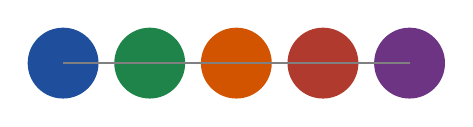
\begin{tikzpicture}
  \foreach \i/\c in {0/mlblue,1/mlgreen,2/mlorange,3/mlred,4/mlpurple}
    \fill[\c] (\i*1.1,0) circle (0.45);
  \draw[thick,gray] (0,0)--(1.1,0)--(2.2,0.0)--(3.3,0)--(4.4,0);
\end{tikzpicture}\\[1.5cm]
{\large A textbook for BCA students\\ Course code NBCA-601}\\[3cm]
{\small Unit I Introduction $\cdot$ Unit II Supervised Learning $\cdot$ Unit III Ensembles \& SVM\\
Unit IV Unsupervised Learning $\cdot$ Unit V Neural Networks}
\end{titlepage}
\chapter*{Preface}
\markboth{Preface}{Preface}
\addcontentsline{toc}{chapter}{Preface}

\textbf{To the student.}

Machine learning is the science of teaching computers to learn from data instead of programming every rule by hand. It sits behind the spam filter in your e-mail, the recommendations on your phone, the translation of a web page and the face unlock of your camera. It is also a subject that can look frightening: it mixes statistics, linear algebra, calculus and programming.

This book was written to make that mixture \textbf{easy to understand}. It follows the syllabus \textbf{NBCA-601 Machine Learning} of the BCA programme topic by topic, and it is organised around one idea:

\begin{center}
\emph{First understand it with a picture and an everyday story, then see the definition, then solve a small example by hand, and only then look at the code.}
\end{center}

\paragraph{What makes this book different.}
\begin{itemize}
  \item \textbf{Every method has a plain-language idea first}: a pizza-shop story for K-Means, a mayor building the widest road for SVMs, a detective multiplying clues for Naive Bayes, a conveyor belt for data pipelines.
  \item \textbf{Every method is defined in exam style} (a definition box you can copy into an answer) and finishes with a clear list of \textbf{advantages, disadvantages and applications}.
  \item \textbf{Every important algorithm is solved by hand, end to end}, with small numbers you can check on paper: a regression line, a perceptron, a decision tree, K-Means, PCA, backpropagation.
  \item \textbf{Every figure is explained.} Below each picture a box called \emph{Reading the Figure} says what the axes, colours and arrows mean.
  \item \textbf{Every chapter ends with an Exam Corner}: questions of 2, 5 and 10 marks with model answers, numerical problems with answers, multiple-choice questions, practice problems and a one-page quick-revision table.
  \item \textbf{All the numbers from Python are real.} Every table of results was produced by running the code shown (Python $3.13$, scikit-learn $1.9$, NumPy $2.5$, TensorFlow $2.21$, Keras $3.15$). Where a result is a schematic illustration and not a real run, the caption says so.
\end{itemize}

\paragraph{How the book is organised.} The ten chapters match the five units of the syllabus, two chapters per unit:

\begin{center}
\begin{tabular}{@{}cp{5.2cm}p{6.3cm}@{}}
\toprule
\textbf{Unit} & \textbf{Theme} & \textbf{Chapters}\\
\midrule
I & Introduction and statistical learning & 1~Introduction to ML, 2~Statistical Learning\\
II & Supervised learning & 3~k-NN, Decision Trees, Naive Bayes; 4~Linear Models and SVM basics\\
III & Ensembles, SVM and Naive Bayes & 5~Ensemble Learning; 6~SVMs and Naive Bayes Classifiers\\
IV & Unsupervised learning & 7~Clustering; 8~Dimensionality Reduction and PCA\\
V & Neural networks & 9~ANNs and MLPs with Keras; 10~TensorFlow and Data Pipelines\\
\bottomrule
\end{tabular}
\end{center}

\paragraph{What you need.} School-level algebra, a little knowledge of probability and Python programming. The few extra mathematical ideas (mean and variance, derivatives, matrices) are explained when they first appear. You do not need a powerful computer: all examples run on an ordinary laptop (the Fashion-MNIST network of Chapter~9 trains in a few minutes on a CPU).

\paragraph{A request.} Do not only read. Take a pencil and \emph{redo the worked examples without looking}, then run the Python code and change the numbers. Machine learning, like swimming, is learned by doing.

\begin{warning}
\textbf{About this edition.} This draft was written with the help of an AI assistant (Claude). All numerical examples were checked by hand, and every Python result was obtained by running the code, but you should still verify important facts, definitions and notation against the textbooks and lecture notes prescribed by your university, and use this book together with them. Please report errors to your teacher so that they can be corrected.
\end{warning}

\vspace{1em}
\begin{flushright}
\emph{Happy learning!}
\end{flushright}

\chapter*{How to Use This Book}
\markboth{How to Use This Book}{How to Use This Book}
\addcontentsline{toc}{chapter}{How to Use This Book}

Every chapter uses the same coloured boxes, so that you always know what you are reading. Here is the legend.

\begin{objectives}
\textbf{Learning Objectives}: opens every chapter and lists exactly what you will be able to do at the end. Use it as a checklist when you revise.
\end{objectives}

\begin{pullquote}[--- a famous person]
Each chapter also starts with a short quotation to set the mood.
\end{pullquote}

\begin{keyidea}
\textbf{Key Idea}: the one thing to remember. If you remember nothing else from a section, remember this box.
\end{keyidea}

\begin{definition}[: Term]
\textbf{Definition}: the formal statement of a concept, written in the form you can copy into an exam answer.
\end{definition}

\begin{example}[: Worked example]
\textbf{Example}: a small problem solved step by step with real numbers. Cover the solution and try it yourself first.
\end{example}

\begin{explain}
\textbf{Reading the Figure}: explains what every axis, colour, arrow and symbol of the picture above means, and what you should conclude from it.
\end{explain}

\begin{warning}
\textbf{Common Mistake}: errors students often make, and how to avoid them.
\end{warning}

\begin{tryit}
\textbf{Try It Yourself}: short Python programs with their real outputs. Run them, change the numbers, and watch what happens.
\end{tryit}

\begin{exam}
\textbf{Exam Tip}: how a topic is usually asked and how to answer it for full marks.
\end{exam}

\procon{Name of the method}
{\item Each method ends with this strip
 \item Advantages: what the method is good at}
{\item Disadvantages: where it fails or what it costs}
{\item Applications: where it is used in practice}

\begin{modelans}[: example]
\textbf{Model Answer}: a complete or outline answer to one of the exam questions, showing the expected structure.
\end{modelans}

\begin{revision}
\textbf{Quick Revision}: a one-page table at the end of every chapter that summarises every topic in one line. Read it the night before the exam.
\end{revision}

\begin{summary}
\textbf{Chapter Summary}: the main points of the chapter in a short list, placed before the Exam Corner.
\end{summary}

\paragraph{The cartoon characters.} Faces and speech bubbles appear in many figures. A smiling face means ``this works well'', a worried face means ``this is a problem'', and an angry face means ``strict'' or ``blame''. Do not skip them: they carry the idea of the picture.

\paragraph{Colours in figures.} Blue, orange and green are used for the classes or clusters; red usually marks errors, boundaries or the thing to notice; purple marks the method's own steps.

\chapter*{Study Guide}
\markboth{Study Guide}{Study Guide}
\addcontentsline{toc}{chapter}{Study Guide}

This guide shows you \emph{where} each part of the syllabus is covered, \emph{how} to study a chapter, and \emph{how} to write answers that earn full marks.

%====================================================================
\section*{1.\ Course Outcomes and Where They Are Covered}

After completing the course the student should be able to do the following (course outcomes of NBCA-601):

\begin{center}
\small
\begin{tabular}{@{}cp{7.6cm}p{4.6cm}@{}}
\toprule
\textbf{CO} & \textbf{Course outcome} & \textbf{Where to study it}\\
\midrule
CO1 & Explain the fundamental usage of the concept of a Machine Learning system & Chapter~\ref{ch:intro} (p.~\pageref{ch:intro}), Chapter~\ref{ch:stat} (p.~\pageref{ch:stat})\\
CO2 & Demonstrate various regression techniques & Chapter~\ref{ch:linear} (p.~\pageref{ch:linear}); also SVM regression in Chapter~\ref{ch:svm}\\
CO3 & Analyse the ensemble learning methods & Chapter~\ref{ch:ensemble} (p.~\pageref{ch:ensemble})\\
CO4 & Illustrate clustering techniques and dimensionality-reduction models & Chapter~\ref{ch:cluster} (p.~\pageref{ch:cluster}), Chapter~\ref{ch:dimred} (p.~\pageref{ch:dimred})\\
CO5 & Discuss neural-network models and the fundamental concepts of deep learning & Chapter~\ref{ch:ann} (p.~\pageref{ch:ann}), Chapter~\ref{ch:tf} (p.~\pageref{ch:tf})\\
\bottomrule
\end{tabular}
\end{center}

%====================================================================
\section*{2.\ Syllabus Map: Every Topic and Its Chapter}

Tick each topic when you can \emph{define it, explain it with a diagram, and solve a numerical example}.

\begin{center}
\small
\begin{tabular}{@{}c p{8.8cm} c c@{}}
\toprule
\textbf{Unit} & \textbf{Syllabus topic} & \textbf{Chapter} & \textbf{Page}\\
\midrule
I & Artificial Intelligence, Machine Learning, types of ML systems, challenges of ML & \ref{ch:intro} & \pageref{ch:intro}\\
I & Statistical learning: supervised and unsupervised learning, training and test loss, trade-offs, estimating risk statistics, sampling distribution of an estimator & \ref{ch:stat} & \pageref{ch:stat}\\
\midrule
II & Distance-based methods, nearest neighbours, decision trees, Naive Bayes & \ref{ch:knn} & \pageref{ch:knn}\\
II & Linear models: linear regression, logistic regression, generalised linear models, support vector machines, binary classification & \ref{ch:linear} & \pageref{ch:linear}\\
\midrule
III & Ensemble learning: voting classifiers, bagging and pasting, random forests, boosting, stacking & \ref{ch:ensemble} & \pageref{ch:ensemble}\\
III & Support vector machines: linear and non-linear SVM classification, SVM regression; Naive Bayes classifiers & \ref{ch:svm} & \pageref{ch:svm}\\
\midrule
IV & Clustering, K-Means and its limits, image segmentation, preprocessing, semi-supervised learning, DBSCAN, Gaussian mixtures & \ref{ch:cluster} & \pageref{ch:cluster}\\
IV & Dimensionality reduction: curse of dimensionality, main approaches, PCA & \ref{ch:dimred} & \pageref{ch:dimred}\\
\midrule
V & Introduction to artificial neural networks with Keras; implementing MLPs with Keras & \ref{ch:ann} & \pageref{ch:ann}\\
V & TensorFlow; loading and preprocessing data with TensorFlow & \ref{ch:tf} & \pageref{ch:tf}\\
\bottomrule
\end{tabular}
\end{center}

\paragraph{Core topics of each unit.} These are the ideas on which most questions are built; make sure you can handle every one of them.

\begin{center}
\small
\begin{tabular}{@{}cp{13.2cm}@{}}
\toprule
\textbf{Unit} & \textbf{Core topics}\\
\midrule
I & Mitchell's definition $(T,P,E)$; supervised / unsupervised / semi-supervised / reinforcement learning; batch vs.\ online; instance- vs.\ model-based; overfitting and underfitting; bias--variance trade-off; training vs.\ test loss; k-fold cross-validation; precision, recall, $F_1$; standard error and the central limit theorem\\
II & k-NN with a numerical example; entropy, information gain and ID3; Naive Bayes with Laplace smoothing; least-squares line and $R^2$; gradient descent; logistic regression (sigmoid, odds, log-loss); GLMs; SVM margin and support vectors\\
III & Bagging vs.\ boosting; random forest; AdaBoost; gradient boosting; stacking; the kernel trick (polynomial and RBF); effect of $C$ and $\gamma$; SVM regression ($\varepsilon$-tube); Gaussian, multinomial and Bernoulli Naive Bayes\\
IV & K-Means (algorithm and example); elbow and silhouette; limits of K-Means; DBSCAN (core, border, noise); Gaussian mixtures and EM; curse of dimensionality; PCA by hand and explained variance\\
V & Perceptron and the XOR problem; MLP forward pass; activation functions; backpropagation; Keras workflow; overfitting control (dropout, L2, early stopping); \texttt{tf.data} pipeline; preprocessing layers\\
\bottomrule
\end{tabular}
\end{center}

%====================================================================
\section*{3.\ How to Study a Chapter (7 Steps)}

\begin{enumerate}
  \item \textbf{Read the Learning Objectives} and turn them into questions you must be able to answer.
  \item \textbf{Read the cartoon or story first.} Do not memorise anything yet; just understand the idea.
  \item \textbf{Study the definition boxes} and copy each definition by hand once. Definitions are the easiest marks in the exam.
  \item \textbf{Redo every worked example} on paper without looking at the solution, then compare.
  \item \textbf{Run the Python code} (or at least read the printed results) and change one number to see the effect.
  \item \textbf{Attempt the Exam Corner} before reading the model answers: first the 2-mark questions, then 5-mark, then 10-mark, then the numericals.
  \item \textbf{Finish with the Quick Revision table}; turn each row into a flash-card.
\end{enumerate}

\begin{center}
\begin{tabular}{@{}p{2.8cm}p{4.2cm}p{6.2cm}@{}}
\toprule
\textbf{Time per chapter} & \textbf{Reading and examples} & \textbf{Practice}\\
\midrule
About 8--10 hours & 4 hours (steps 1--4) & 1 hour of code (step 5), 3--4 hours of Exam Corner (steps 6--7)\\
\bottomrule
\end{tabular}
\end{center}

\subsection*{A suggested 15-week plan}

\begin{center}
\small
\begin{tabular}{@{}p{2.2cm}p{4.3cm}p{7.2cm}@{}}
\toprule
\textbf{Week} & \textbf{Chapter} & \textbf{Focus}\\
\midrule
1 & Chapter~\ref{ch:intro} & types of ML, overfitting, the vocabulary\\
2--3 & Chapter~\ref{ch:stat} & loss, bias--variance, cross-validation, standard error\\
4 & Chapter~\ref{ch:knn} & k-NN, decision tree by hand, Naive Bayes by hand\\
5 & Chapter~\ref{ch:linear} & regression line, gradient descent, logistic regression, SVM idea\\
6 & Chapter~\ref{ch:ensemble} & bagging, random forest, AdaBoost by hand\\
7 & Chapter~\ref{ch:svm} & kernels, soft margin, SVR, Naive Bayes variants\\
8 & Chapter~\ref{ch:cluster} & K-Means by hand, DBSCAN, EM\\
9 & Chapter~\ref{ch:dimred} & curse of dimensionality, PCA by hand\\
10 & Chapter~\ref{ch:ann} & perceptron, forward pass, backpropagation, Keras\\
11 & Chapter~\ref{ch:tf} & tensors, \texttt{GradientTape}, \texttt{tf.data}\\
12--13 & Revision & Quick Revision tables, formula sheet (Appendix~A), MCQs of all chapters\\
14 & Mock test & answer a full paper in the time allowed, using the answer-writing guide below\\
15 & Final revision & glossary (Appendix~B), weak topics only\\
\bottomrule
\end{tabular}
\end{center}

%====================================================================
\section*{4.\ How to Write Answers That Earn Full Marks}

\subsection*{The structure of an answer}

\begin{center}
\small
\begin{tabular}{@{}p{2.3cm}p{9.0cm}p{2.3cm}@{}}
\toprule
\textbf{Marks} & \textbf{What to write} & \textbf{Time}\\
\midrule
\textbf{2 marks} & a precise \textbf{definition} (2--3 lines) plus one key fact, formula or example & 2--3 min\\
\textbf{5 marks} & definition $+$ a \textbf{labelled diagram} (or table) $+$ 4--5 points of explanation $+$ one short example or formula & 8--10 min\\
\textbf{10 marks} & introduction $+$ definition $+$ \textbf{working or algorithm in steps} $+$ \textbf{diagram} $+$ \textbf{worked numerical example} $+$ advantages and disadvantages $+$ applications $+$ a one-line conclusion & 15--20 min\\
\textbf{Numerical} & write ``Given'', the \textbf{formula}, the \textbf{substitution}, the calculation \textbf{step by step}, and the final answer with its meaning & as needed\\
\bottomrule
\end{tabular}
\end{center}

\subsection*{The same topic at three different lengths}

\textbf{Topic: Overfitting.}

\begin{itemize}
  \item \textbf{2 marks.} \emph{Overfitting} occurs when a model fits the training data, including its noise, so well that it performs poorly on new data (low training error, high test error). It is caused by a model that is too complex for the amount of data.
  \item \textbf{5 marks.} Add: (i)~a diagram of three fits (underfit, good fit, overfit); (ii)~causes: complex model, little or noisy data, too many features; (iii)~how to detect it: large gap between training and validation error; (iv)~remedies: more data, simpler model, regularisation, cross-validation, early stopping, pruning; (v)~an example, such as a degree-9 polynomial through ten points.
  \item \textbf{10 marks.} Add: the bias--variance explanation ($\text{error}=\text{bias}^2+\text{variance}+\sigma^2$, overfitting $=$ high variance), the curve of training and test error against model complexity, a numerical example (e.g.\ train MSE $0.026$ vs.\ test MSE $0.102$ for degree 9), and a comparison table with underfitting.
\end{itemize}

\subsection*{A checklist before you finish an answer}

\begin{enumerate}
  \item Did I give the \textbf{definition} in the textbook's words?
  \item Did I draw a \textbf{neat, labelled diagram} (axes, classes, arrows) where one is useful?
  \item Did I write the \textbf{formula} and explain every symbol?
  \item Did I include a \textbf{small example}, with numbers?
  \item Did I mention \textbf{advantages, disadvantages and applications} when asked about a method?
  \item For a comparison, did I use a \textbf{table} with at least four points?
  \item For a numerical, did I show \textbf{all steps} and the final answer?
\end{enumerate}

\begin{exam}
Draw diagrams with a pencil and ruler, label every axis, and use different markers (circle, triangle) for different classes. A clear diagram is often worth as many marks as a paragraph of text.
\end{exam}

\subsection*{Common mistakes of students}

\begin{center}
\small
\begin{tabular}{@{}p{6.4cm}p{6.9cm}@{}}
\toprule
\textbf{Mistake} & \textbf{Correct habit}\\
\midrule
Writing ``K-Means needs labels'' & K-Means is \emph{unsupervised}: no labels\\
Confusing parameters and hyperparameters & parameters are \emph{learned}; hyperparameters are \emph{set by you}\\
Reporting training accuracy as model performance & always report \textbf{test} (or validation) performance\\
Scaling the whole dataset before splitting & compute scaling statistics on the \textbf{training set only}\\
Forgetting to scale features for k-NN, SVM, PCA, neural networks & always scale distance-based and gradient-based methods\\
Mixing up bagging and boosting & bagging: parallel, reduces \emph{variance}; boosting: sequential, reduces \emph{bias}\\
Leaving numerical answers without units or meaning & write a sentence: ``so the student is predicted to \dots''\\
\bottomrule
\end{tabular}
\end{center}

\chapter*{Notation}
\markboth{Notation}{Notation}
\addcontentsline{toc}{chapter}{Notation}

The same symbols are used throughout the book. Vectors are bold lower-case letters, matrices are bold upper-case letters.

\small
\begin{longtable}{@{}p{2.6cm}p{11.4cm}@{}}
\toprule
\textbf{Symbol} & \textbf{Meaning}\\
\midrule
\endhead
$n$ & number of training instances\\
$d$, $p$ & number of features (dimension of the input)\\
$m$, $k$, $K$ & number of components kept (PCA), number of clusters or neighbours, number of classes or mixture components\\
$\vect x$, $x_j$ & feature vector of an instance; its $j$-th feature\\
$\mathbf X$ & data matrix with $n$ rows (instances) and $d$ columns (features)\\
$y$, $\hat y$ & true target (label) and predicted target\\
$f$, $\hat f$ & true (unknown) function and its estimate (the model)\\
$\varepsilon$, $\sigma^2$ & random error (noise) and its variance; also the radius in DBSCAN and the tube half-width in SVR\\
$\vect w$, $\vect\theta$, $b$ & weights (parameters) and bias (intercept)\\
$\eta$, $\alpha$ & learning rate (also written $\eta$); $\alpha$ is also the Laplace smoothing constant, the dual variable in SVMs and the leaky-ReLU slope\\
$\lambda$ & regularisation strength; eigenvalue (PCA, covariance matrix)\\
$C$ & SVM penalty for margin violations\\
$\gamma$ & kernel width in the RBF kernel; discount factor in reinforcement learning\\
$\xi_i$ & slack variable\\
$J$, $L$, $\Risk$ & loss (cost) function; loss of one example; risk (expected loss)\\
$\E[\cdot]$, $\Var$, $\SE$ & expectation, variance, standard error\\
$\mu$, $\sigma$, $\bar x$, $s$ & population mean and standard deviation; sample mean and standard deviation\\
$\mathcal N(\mu,\sigma^2)$ & normal (Gaussian) distribution\\
$\mathbf\Sigma$, $\mathbf C$ & covariance matrix\\
$P(\cdot)$, $P(\cdot\mid\cdot)$ & probability and conditional probability\\
$z$, $a$, $\varphi$ & pre-activation $z=\vect w\cdot\vect x+b$, activation $a=\varphi(z)$, activation function\\
$\sigma(z)$ & sigmoid function $1/(1+e^{-z})$ (context distinguishes it from a standard deviation)\\
$\delta^{(l)}$ & error signal of layer $l$ in backpropagation\\
$\|\vect a\|$ & Euclidean length (norm) of $\vect a$\\
$\vect a\cdot\vect b$ & dot product\\
$\argmax$, $\argmin$ & the argument that gives the maximum, minimum\\
$\mathbb 1[\cdot]$ & indicator: 1 if the condition is true, 0 otherwise\\
TP, FP, TN, FN & true/false positives and negatives in a confusion matrix\\
\bottomrule
\end{longtable}

\tableofcontents
\mainmatter
\chapter{Introduction to Machine Learning}

\begin{objectives}
After this chapter you will be able to:
\begin{itemize}
  \item explain the difference between \textbf{AI, Machine Learning and Deep Learning};
  \item define Machine Learning using Tom Mitchell's $(T,P,E)$ definition;
  \item classify ML systems as \textbf{supervised, unsupervised, semi-supervised} or \textbf{reinforcement};
  \item distinguish \textbf{batch vs.\ online} and \textbf{instance-based vs.\ model-based} learning;
  \item list and explain the main \textbf{challenges} of ML, especially \textbf{overfitting} and \textbf{underfitting};
  \item train your first model in Python in under ten lines.
\end{itemize}
\end{objectives}

\begin{pullquote}[--- Arthur Samuel, 1959]
Machine learning is the field of study that gives computers the ability to learn without being explicitly programmed.
\end{pullquote}

\section{Why Do We Need Machine Learning?}

Imagine you must write a program that detects \emph{spam e-mail}. The traditional way is to write rules by hand:

\begin{itemize}
  \item If the subject contains ``FREE'' $\Rightarrow$ spam.
  \item If the sender is unknown and the mail contains ``winner'' $\Rightarrow$ spam.
  \item If \ldots{} (hundreds more rules)
\end{itemize}

Spammers quickly change their words (``FR33'', ``fr.ee'') and your rule list becomes long, fragile and impossible to maintain. A \textbf{machine-learning} program instead looks at thousands of mails already labelled as spam or not-spam and \emph{discovers the pattern by itself}. When spammers change tactics, we simply retrain it on new data.

\begin{center}
\resizebox{\linewidth}{!}{%
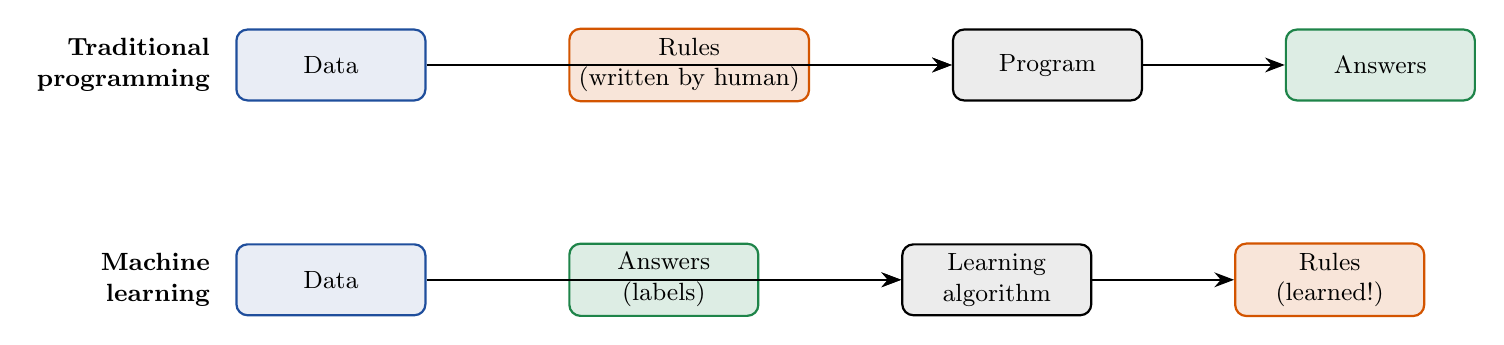
\begin{tikzpicture}[node distance=1.6cm and 1.8cm,
  box/.style={draw,rounded corners,minimum width=2.4cm,minimum height=0.9cm,align=center,font=\small,thick},
  arr/.style={-{Stealth[length=2.5mm]},thick}]
% traditional
\node[box,fill=mlblue!10,draw=mlblue] (d1) {Data};
\node[box,fill=mlorange!15,draw=mlorange,right=of d1] (r1) {Rules\\(written by human)};
\node[box,fill=gray!15,right=of r1] (p1) {Program};
\node[box,fill=mlgreen!15,draw=mlgreen,right=of p1] (o1) {Answers};
\draw[arr] (d1)--(p1); \draw[arr] (r1)--(p1); \draw[arr] (p1)--(o1);
\node[left=0.2cm of d1,align=right,font=\bfseries\small] {Traditional\\programming};
% ML
\node[box,fill=mlblue!10,draw=mlblue,below=1.8cm of d1] (d2) {Data};
\node[box,fill=mlgreen!15,draw=mlgreen,right=of d2] (a2) {Answers\\(labels)};
\node[box,fill=gray!15,right=of a2] (p2) {Learning\\algorithm};
\node[box,fill=mlorange!15,draw=mlorange,right=of p2] (r2) {Rules\\(learned!)};
\draw[arr] (d2)--(p2); \draw[arr] (a2)--(p2); \draw[arr] (p2)--(r2);
\node[left=0.2cm of d2,align=right,font=\bfseries\small] {Machine\\learning};
\end{tikzpicture}}
\end{center}

\begin{keyidea}
In traditional programming, humans supply \emph{data + rules} and get \emph{answers}.
In machine learning, humans supply \emph{data + answers} and the computer finds the \emph{rules}.
\end{keyidea}

\section{Artificial Intelligence, Machine Learning and Deep Learning}

These three terms are often mixed up. They are nested, like Russian dolls.

\begin{center}
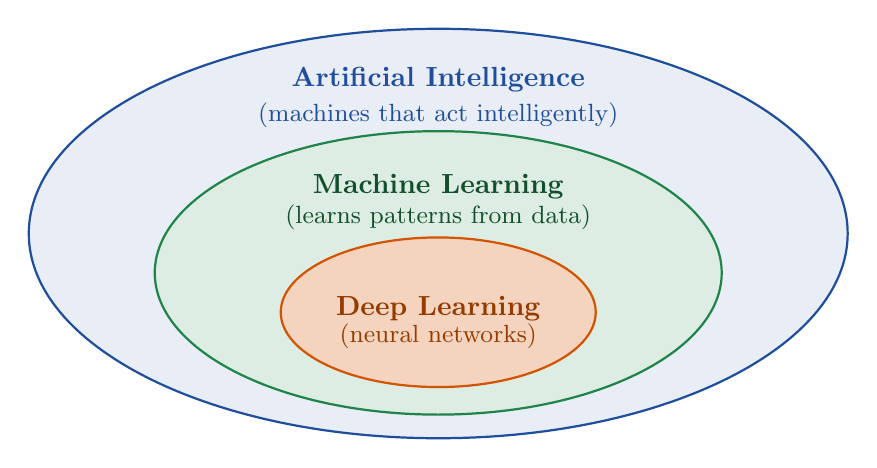
\begin{tikzpicture}
\draw[fill=mlblue!10,draw=mlblue,thick] (0,0) ellipse (5.2 and 2.6);
\draw[fill=mlgreen!15,draw=mlgreen,thick] (0,-0.5) ellipse (3.6 and 1.8);
\draw[fill=mlorange!25,draw=mlorange,thick] (0,-1.0) ellipse (2.0 and 0.95);
\node[font=\bfseries,mlblue] at (0,1.95) {Artificial Intelligence};
\node[font=\small,mlblue] at (0,1.5) {(machines that act intelligently)};
\node[font=\bfseries,mlgreen!60!black] at (0,0.6) {Machine Learning};
\node[font=\small,mlgreen!60!black] at (0,0.2) {(learns patterns from data)};
\node[font=\bfseries,mlorange!70!black] at (0,-0.95) {Deep Learning};
\node[font=\small,mlorange!70!black] at (0,-1.3) {(neural networks)};
\end{tikzpicture}
\end{center}

\begin{definition}[: Artificial Intelligence]
\textbf{Artificial Intelligence (AI)} is the science of building machines that perform tasks that normally require human intelligence, such as reasoning, understanding language, recognising images and making decisions.
\end{definition}

\begin{definition}[: Machine Learning]
A computer program is said to \textbf{learn} from experience $E$ with respect to some class of tasks $T$ and performance measure $P$, if its performance at tasks in $T$, as measured by $P$, improves with experience $E$. \hfill (Tom Mitchell, 1997)
\end{definition}

\begin{example}[: Spam filter in $(T,P,E)$ form]
\begin{center}
\begin{tabular}{@{}ll@{}}
\toprule
\textbf{Task $T$} & Flag new e-mails as spam or not spam\\
\textbf{Performance $P$} & Percentage of e-mails classified correctly (accuracy)\\
\textbf{Experience $E$} & A collection of e-mails labelled by users\\
\bottomrule
\end{tabular}
\end{center}
If accuracy rises as we feed in more labelled mail, the program is \emph{learning}.
\end{example}

\begin{exam}
``Define Machine Learning'' appears almost every year. Write \emph{both} Samuel's one-line definition and Mitchell's $(T,P,E)$ definition, then give the spam-filter example. This earns full marks.
\end{exam}

\section{Where Is Machine Learning Used?}

\begin{center}
\begin{tabular}{@{}p{3.6cm}p{5.2cm}p{4.6cm}@{}}
\toprule
\textbf{Area} & \textbf{Application} & \textbf{ML task}\\
\midrule
\faEnvelope\ E-mail & Spam filtering & Classification\\
\faShoppingCart\ E-commerce & ``Customers also bought'' & Recommendation\\
\faHeartbeat\ Health & Detecting disease from X-rays & Image classification\\
\faCar\ Transport & Self-driving cars & Perception, control\\
\faLanguage\ Language & Google Translate, chatbots & Sequence modelling\\
\faChartLine\ Finance & Credit-card fraud detection & Anomaly detection\\
\faHome\ Real estate & Predicting house price & Regression\\
\bottomrule
\end{tabular}
\end{center}

\section{Types of Machine Learning Systems}

We classify ML systems using three independent questions.

\begin{enumerate}[label=\textbf{Q\arabic*.}]
  \item Is it trained with human supervision? (supervised, unsupervised, semi-supervised, reinforcement)
  \item Can it learn on the fly? (batch vs.\ online)
  \item Does it compare with known data or build a model? (instance-based vs.\ model-based)
\end{enumerate}

\subsection{Supervised Learning}

The training data includes the \textbf{answer} (called a \emph{label} or \emph{target}). It is like studying with an answer key.

\begin{definition}[: Supervised Learning]
Given training examples $\{(\vect{x}_i, y_i)\}_{i=1}^{n}$, where $\vect{x}_i$ is the input (features) and $y_i$ the correct output (label), learn a function $f$ such that $f(\vect{x}) \approx y$ on new, unseen inputs.
\end{definition}

There are two main kinds of supervised task:

\begin{center}
\begin{tabular}{@{}lll@{}}
\toprule
 & \textbf{Classification} & \textbf{Regression}\\
\midrule
Output $y$ is & a \emph{category} & a \emph{number}\\
Example & spam / not spam & price of a house\\
Typical algorithms & k-NN, Naive Bayes, SVM & Linear regression\\
\bottomrule
\end{tabular}
\end{center}

\begin{center}
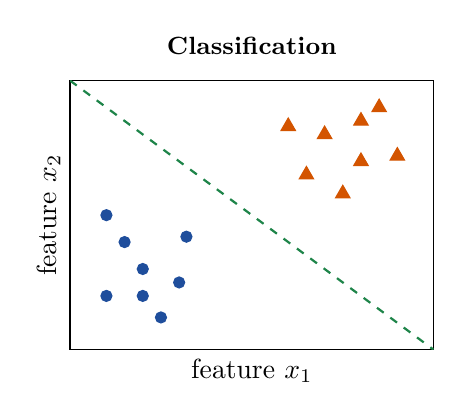
\begin{tikzpicture}
\begin{axis}[width=6.2cm,height=5cm,title={\textbf{Classification}},xlabel={feature $x_1$},ylabel={feature $x_2$},
  xmin=0,xmax=10,ymin=0,ymax=10,ticks=none,title style={font=\small}]
\addplot[only marks,mark=*,mlblue,mark size=2pt] coordinates {(1,2)(2,3)(1.5,4)(3,2.5)(2.5,1.2)(1,5)(3.2,4.2)(2,2)};
\addplot[only marks,mark=triangle*,mlorange,mark size=3pt] coordinates {(7,8)(8,7)(6.5,6.5)(8.5,9)(7.5,5.8)(9,7.2)(6,8.3)(8,8.5)};
\addplot[dashed,thick,mlgreen,domain=0:10] {10-x};
\end{axis}
\end{tikzpicture}\hfill
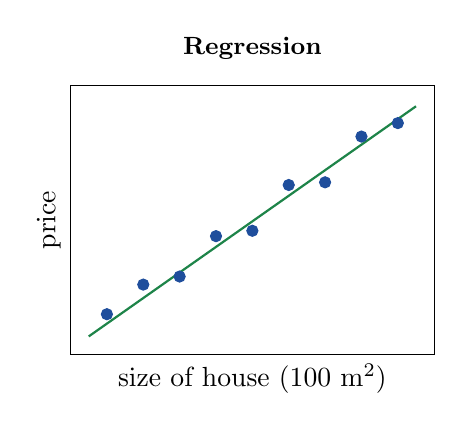
\begin{tikzpicture}
\begin{axis}[width=6.2cm,height=5cm,title={\textbf{Regression}},xlabel={size of house (100 m$^2$)},ylabel={price},
  xmin=0,xmax=10,ymin=0,ymax=10,ticks=none,title style={font=\small}]
\addplot[only marks,mark=*,mlblue,mark size=2pt] coordinates {(1,1.5)(2,2.6)(3,2.9)(4,4.4)(5,4.6)(6,6.3)(7,6.4)(8,8.1)(9,8.6)};
\addplot[thick,mlgreen,domain=0.5:9.5] {0.95*x+0.2};
\end{axis}
\end{tikzpicture}
\end{center}

\subsection{Unsupervised Learning}

The training data is \textbf{unlabelled}; the system must find structure on its own, like sorting a pile of unknown coins into groups.

\begin{itemize}
  \item \textbf{Clustering:} group similar customers (e.g.\ K-Means, DBSCAN) --- Unit IV.
  \item \textbf{Dimensionality reduction:} compress many features into few (e.g.\ PCA) --- Unit IV.
  \item \textbf{Anomaly detection:} spot unusual credit-card transactions.
  \item \textbf{Association rules:} ``people who buy bread also buy butter''.
\end{itemize}

\subsection{Semi-supervised Learning}

Labelling data is expensive, so we label \emph{a little} and leave most unlabelled. Google Photos is a classic case: it clusters faces automatically (unsupervised) and you type a name once per person (supervised).

\subsection{Reinforcement Learning}

An \textbf{agent} observes an environment, takes \textbf{actions}, and receives \textbf{rewards} or penalties. It learns a \emph{policy} that maximises total reward, as when a robot learns to walk or AlphaGo learns Go.

\begin{center}
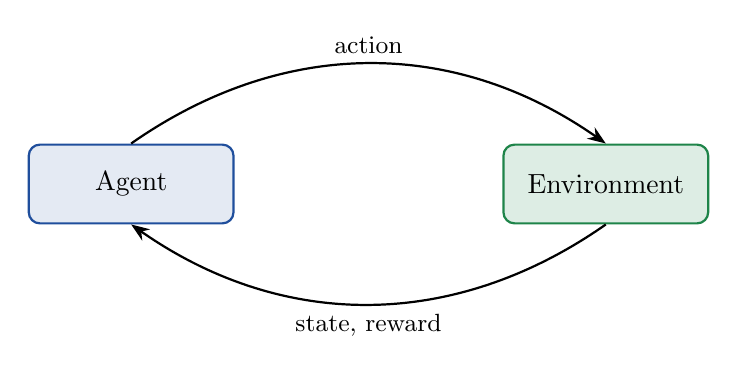
\begin{tikzpicture}[node distance=3.4cm,
  box/.style={draw,rounded corners,thick,minimum width=2.6cm,minimum height=1cm,align=center},
  arr/.style={-{Stealth},thick}]
\node[box,fill=mlblue!12,draw=mlblue] (a) {Agent};
\node[box,fill=mlgreen!15,draw=mlgreen,right=of a] (e) {Environment};
\draw[arr] (a.north) to[bend left=35] node[above,font=\small]{action} (e.north);
\draw[arr] (e.south) to[bend left=35] node[below,font=\small]{state, reward} (a.south);
\end{tikzpicture}
\end{center}

\begin{center}
\begin{tabular}{@{}lccc@{}}
\toprule
\textbf{Type} & \textbf{Labels?} & \textbf{Feedback} & \textbf{Typical use}\\
\midrule
Supervised & Yes & Correct answer & Spam detection, price prediction\\
Unsupervised & No & None & Customer segmentation\\
Semi-supervised & Few & Partial & Photo tagging\\
Reinforcement & No & Reward / penalty & Games, robotics\\
\bottomrule
\end{tabular}
\end{center}

\subsection{Batch vs.\ Online Learning}

\begin{description}
  \item[Batch (offline):] trained once on \emph{all} the data, then deployed. To learn new data you retrain from scratch.
  \item[Online (incremental):] learns continuously from small mini-batches as data arrives, so it suits stock prices or streaming data and needs less memory. Its \emph{learning rate} controls how fast it forgets old data.
\end{description}

\subsection{Instance-based vs.\ Model-based Learning}

\begin{description}
  \item[Instance-based:] memorises the training examples and predicts for a new point by comparing it with similar ones (e.g.\ k-Nearest Neighbours).
  \item[Model-based:] builds a mathematical model from the examples and then uses \emph{only the model} to predict (e.g.\ linear regression).
\end{description}

\begin{example}[: Does money make people happy?]
Suppose we have data on GDP per capita $x$ and life satisfaction $y$ for several countries, and the points look roughly linear. A model-based approach assumes
\[
  y = \theta_0 + \theta_1 x
\]
and \emph{learns} the best parameters $\theta_0,\theta_1$ from the data. For a new country with GDP $x_{\text{new}}$ we predict $\hat y=\theta_0+\theta_1x_{\text{new}}$ and never look at the training data again.
\end{example}

\begin{tryit}
Your first model, using the \texttt{scikit-learn} library:
\begin{lstlisting}
from sklearn.linear_model import LinearRegression

# Experience E: house size (100 m^2) and price (lakh Rs)
X = [[1], [2], [3], [4], [5]]
y = [15, 26, 29, 44, 46]

model = LinearRegression()       # choose the model
model.fit(X, y)                  # learn theta_0 and theta_1
print(model.intercept_, model.coef_[0])
print(model.predict([[6]]))      # price of a 600 m^2 house?
\end{lstlisting}
\emph{Challenge:} add two more data points and see how the prediction changes.
\end{tryit}

\section{The Machine Learning Workflow}

\begin{center}
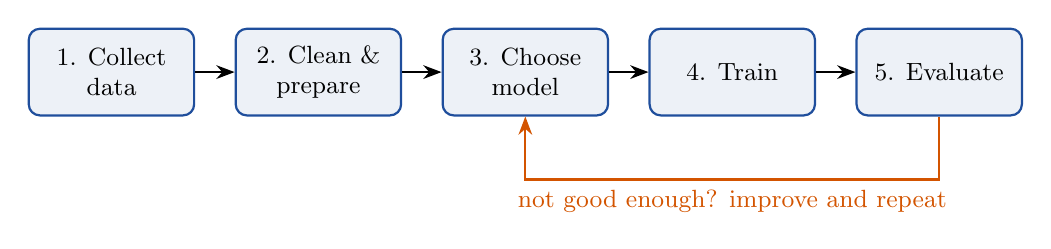
\begin{tikzpicture}[node distance=0.5cm,
  s/.style={draw,rounded corners,thick,minimum width=2.1cm,minimum height=1.1cm,align=center,font=\small,fill=mlblue!8,draw=mlblue},
  arr/.style={-{Stealth},thick}]
\node[s] (1) {1. Collect\\data};
\node[s,right=of 1] (2) {2. Clean \&\\prepare};
\node[s,right=of 2] (3) {3. Choose\\model};
\node[s,right=of 3] (4) {4. Train};
\node[s,right=of 4] (5) {5. Evaluate};
\foreach \a/\b in {1/2,2/3,3/4,4/5} \draw[arr] (\a)--(\b);
\draw[arr,mlorange] (5.south) -- ++(0,-0.8) -| node[pos=0.25,below,font=\small]{not good enough? improve and repeat} (3.south);
\end{tikzpicture}
\end{center}

\section{Main Challenges of Machine Learning}

``What can go wrong?'' falls into two groups: \emph{bad data} and \emph{bad algorithm}.

\subsection{Problems with the data}

\begin{enumerate}
  \item \textbf{Insufficient training data.} Simple tasks need thousands of examples, and complex tasks like image recognition need millions. Banko \& Brill showed that, given enough data, even simple algorithms perform almost as well as sophisticated ones.
  \item \textbf{Non-representative data.} If you survey only rich countries, your model of ``happiness vs.\ money'' fails for poor ones. This is called \textbf{sampling bias}.
  \item \textbf{Poor-quality data.} Errors, outliers and missing values make it hard for the system to see patterns, so data cleaning takes a large share of every ML project.
  \item \textbf{Irrelevant features.} ``Garbage in, garbage out.'' \textbf{Feature engineering} means selecting useful features, extracting new ones by combining old ones, and creating new ones by collecting more data.
\end{enumerate}

\subsection{Problems with the algorithm}

\paragraph{Overfitting.} The model performs great on training data but poorly on new data, because it has \emph{memorised the noise} instead of learning the pattern. It is like a student who memorises last year's paper but cannot solve a new question.

\paragraph{Underfitting.} The model is too simple to capture the underlying pattern, so it does badly even on the training data. It is like a student who read only the chapter titles.

\begin{center}
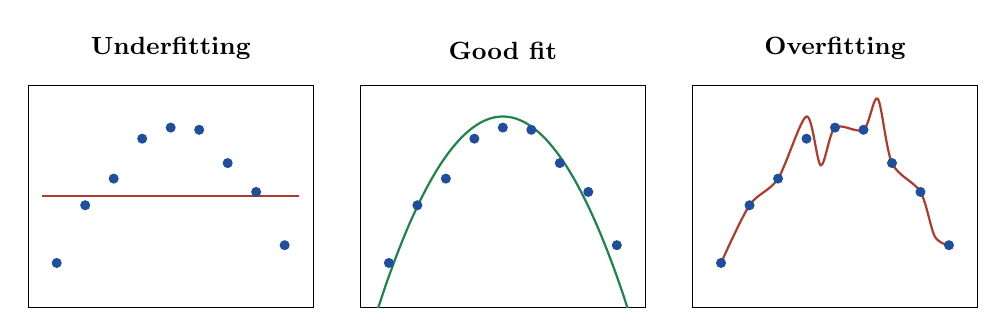
\begin{tikzpicture}
\begin{groupplot}[group style={group size=3 by 1,horizontal sep=0.6cm},width=5.2cm,height=4.4cm,
  xmin=0,xmax=10,ymin=0,ymax=10,ticks=none,title style={font=\small\bfseries}]
\nextgroupplot[title={Underfitting}]
\addplot[only marks,mark=*,mlblue,mark size=1.6pt] coordinates {(1,2)(2,4.6)(3,5.8)(4,7.6)(5,8.1)(6,8.0)(7,6.5)(8,5.2)(9,2.8)};
\addplot[thick,mlred,domain=0.5:9.5]{5};
\nextgroupplot[title={Good fit}]
\addplot[only marks,mark=*,mlblue,mark size=1.6pt] coordinates {(1,2)(2,4.6)(3,5.8)(4,7.6)(5,8.1)(6,8.0)(7,6.5)(8,5.2)(9,2.8)};
\addplot[thick,mlgreen,domain=0.5:9.5,smooth]{-0.45*(x-5)^2+8.6};
\nextgroupplot[title={Overfitting}]
\addplot[only marks,mark=*,mlblue,mark size=1.6pt] coordinates {(1,2)(2,4.6)(3,5.8)(4,7.6)(5,8.1)(6,8.0)(7,6.5)(8,5.2)(9,2.8)};
\addplot[thick,mlred,smooth] coordinates {(1,2)(2,4.6)(3,5.8)(4,8.6)(4.5,6.4)(5,8.1)(6,8.0)(6.5,9.4)(7,6.5)(8,5.2)(8.5,3.2)(9,2.8)};
\end{groupplot}
\end{tikzpicture}
\end{center}

The classic picture below shows what happens as we make the model more complex.

\begin{center}
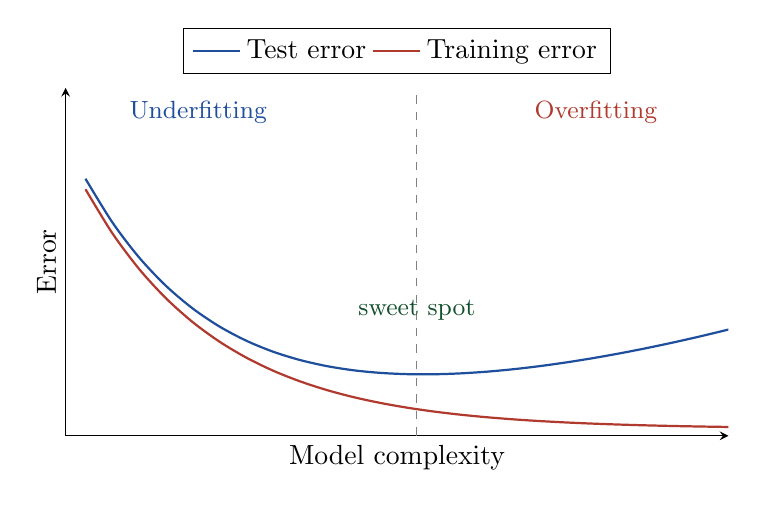
\begin{tikzpicture}
\begin{axis}[width=10cm,height=6cm,xlabel={Model complexity},ylabel={Error},
  xmin=0,xmax=10,ymin=0,ymax=10,ticks=none,legend style={at={(0.5,1.04)},anchor=south,legend columns=2},axis lines=left]
\addplot[thick,mlblue,smooth,domain=0.3:10]{8*exp(-0.5*x)+0.5+0.025*x^2};
\addplot[thick,mlred,smooth,domain=0.3:10]{8*exp(-0.5*x)+0.2};
\legend{Test error, Training error}
\draw[dashed,gray] (axis cs:5.3,0) -- (axis cs:5.3,10);
\node[font=\small,mlblue] at (axis cs:2,9.3) {Underfitting};
\node[font=\small,mlred] at (axis cs:8,9.3) {Overfitting};
\node[font=\small,mlgreen!60!black] at (axis cs:5.3,3.6) {sweet spot};
\end{axis}
\end{tikzpicture}
\end{center}

\begin{warning}
A very high accuracy on training data does \textbf{not} mean the model is good. Always evaluate on data the model has \emph{never seen} (the test set, Chapter 2).
\end{warning}

\begin{center}
\begin{tabular}{@{}p{4cm}p{4.6cm}p{4.6cm}@{}}
\toprule
 & \textbf{Overfitting} & \textbf{Underfitting}\\
\midrule
Model is & too complex & too simple\\
Training error & very low & high\\
Test error & high & high\\
Fixes & more data, simpler model, regularisation, remove noise & more complex model, better features, train longer\\
\bottomrule
\end{tabular}
\end{center}

\begin{keyidea}
The goal of ML is \textbf{generalisation}: performing well on \emph{new} data, not on the data we trained with.
\end{keyidea}

\begin{summary}
\begin{itemize}
  \item AI $\supset$ ML $\supset$ Deep Learning.
  \item ML learns the \emph{rules} from \emph{data}; Mitchell's definition uses $(T,P,E)$.
  \item Systems are classified as supervised, unsupervised, semi-supervised or reinforcement; batch or online; instance-based or model-based.
  \item Challenges: little data, non-representative data, poor quality, irrelevant features, overfitting, underfitting.
  \item The aim is good \textbf{generalisation} to unseen data.
\end{itemize}
\end{summary}

\section*{Review Questions}
\begin{enumerate}
  \item Define Machine Learning. State Mitchell's definition with an example.
  \item Differentiate between AI, ML and Deep Learning with a diagram.
  \item Compare supervised and unsupervised learning with two examples each.
  \item What is the difference between batch and online learning?
  \item Distinguish instance-based and model-based learning.
  \item Explain overfitting and underfitting. How can each be reduced?
  \item List any four challenges of machine learning.
\end{enumerate}

\section*{Practice Problems}
\begin{enumerate}
  \item Identify whether each task is classification, regression or clustering: (a) predicting tomorrow's temperature, (b) deciding if a tumour is benign, (c) grouping news articles by topic.
  \item Write the $(T,P,E)$ description for a handwriting-recognition program.
  \item \textbf{Coding:} extend the \texttt{LinearRegression} example to print the predicted price for sizes 6, 7 and 8.
\end{enumerate}

\chapter{Statistical Learning}

\begin{objectives}
After studying this chapter you will be able to:
\begin{itemize}
  \item describe the statistical model $Y=f(X)+\varepsilon$ and explain \emph{prediction} versus \emph{inference};
  \item state the statistical view of \textbf{supervised} and \textbf{unsupervised} learning;
  \item define and compute common \textbf{loss functions} (squared, absolute, 0--1);
  \item distinguish \textbf{training loss}, \textbf{test loss} and \textbf{risk}, and explain why training loss is optimistic;
  \item derive and interpret the \textbf{bias--variance decomposition} and describe the main \textbf{trade-offs} of statistical learning;
  \item estimate risk using the \textbf{hold-out}, \textbf{k-fold} and \textbf{leave-one-out} methods and compute classification statistics (accuracy, precision, recall, F1);
  \item explain the \textbf{sampling distribution of an estimator}, its bias, variance and standard error, and use the Central Limit Theorem;
  \item answer 2-, 5- and 10-mark university questions on Unit~I.
\end{itemize}
\end{objectives}

\begin{pullquote}[--- George Box]
All models are wrong, but some are useful.
\end{pullquote}

%====================================================================
\section{Introduction to Statistical Learning}

Chapter~1 told us \emph{what} machine learning is. \textbf{Statistical learning} is the mathematical framework that tells us \emph{why it works}, \emph{how well} it works, and \emph{how to measure that}. It treats data as random samples drawn from some unknown real-world process and asks: how can we learn that process from a finite sample?

\subsection{The Statistical Model}

Suppose we observe $p$ input variables $X=(X_1,\dots,X_p)$ (the \emph{features}) and one output variable $Y$ (the \emph{response}). We assume that they are related by
\begin{equation}\label{eq:model}
  Y = f(X) + \varepsilon .
\end{equation}
\begin{itemize}
  \item $f$ is an \textbf{unknown fixed function}: the systematic, predictable part of the relationship.
  \item $\varepsilon$ is a \textbf{random error} (noise) with mean zero, $\E[\varepsilon]=0$, independent of $X$ and with variance $\sigma^2$. It stands for everything we did not measure or that is genuinely random.
\end{itemize}
Statistical learning is therefore \emph{the set of methods for estimating $f$} from data. Our estimate is written $\hat f$.

\begin{figure}[!htbp]
\centering
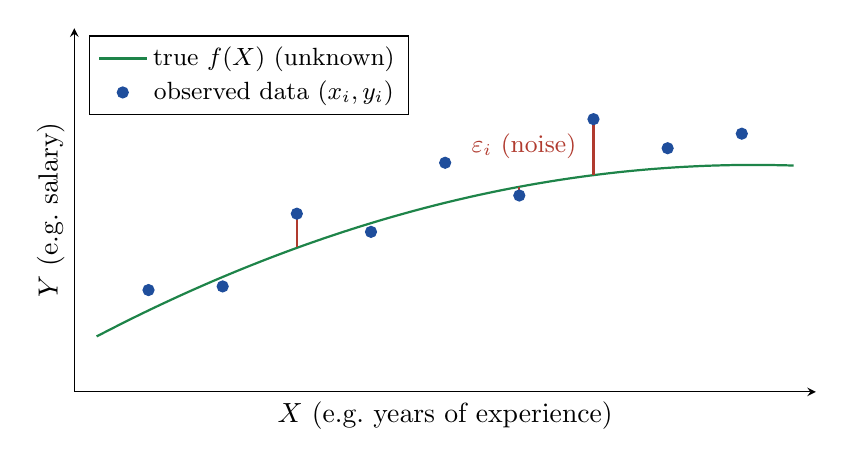
\begin{tikzpicture}
\begin{axis}[width=11cm,height=6.2cm,xlabel={$X$ (e.g.\ years of experience)},ylabel={$Y$ (e.g.\ salary)},
  xmin=0,xmax=10,ymin=0,ymax=10,ticks=none,axis lines=left,
  legend style={at={(0.02,0.98)},anchor=north west,font=\small}]
\addplot[thick,mlgreen,smooth,domain=0.3:9.7]{1.2+1.1*x-0.06*x^2};
\addlegendentry{true $f(X)$ (unknown)}
\addplot[only marks,mark=*,mlblue,mark size=2pt] coordinates {(1,2.8)(2,2.9)(3,4.9)(4,4.4)(5,6.3)(6,5.4)(7,7.5)(8,6.7)(9,7.1)};
\addlegendentry{observed data $(x_i,y_i)$}
\draw[mlred,thick] (axis cs:3,3.99) -- (axis cs:3,4.9);
\draw[mlred,thick] (axis cs:6,5.64) -- (axis cs:6,5.4);
\draw[mlred,thick] (axis cs:7,5.96) -- (axis cs:7,7.5);
\node[mlred,font=\small,anchor=east] at (axis cs:6.9,6.75) {$\varepsilon_i$ (noise)};
\end{axis}
\end{tikzpicture}
\caption{Data are generated as $Y=f(X)+\varepsilon$. The curve is the true but unknown $f$; dots are noisy observations.}\label{fig:model}
\end{figure}

\begin{explain}
The \textbf{green curve} is the true relationship $f(X)$, which in real life we never see. The \textbf{blue dots} are what we actually collect: each dot lies slightly above or below the curve because of random noise. The \textbf{short red vertical segments} are examples of the noise term $\varepsilon_i = y_i - f(x_i)$. Our job is to look only at the dots and recover a curve $\hat f$ as close to the green one as possible. Because of the noise, we can \emph{never} recover $f$ perfectly.
\end{explain}

\subsection{Why Estimate $f$? Prediction and Inference}

\begin{description}
  \item[Prediction.] We only care about getting accurate predictions $\hat Y=\hat f(X)$ for new $X$. $\hat f$ can be a ``black box''. \emph{Example:} forecasting tomorrow's sales.
  \item[Inference.] We want to \emph{understand} how $Y$ changes with each $X_j$: which features matter, whether the effect is positive or negative, and how strong it is. $\hat f$ must be interpretable. \emph{Example:} how much does one extra year of education raise salary?
\end{description}

\paragraph{Reducible and irreducible error.} For a fixed $\hat f$ and $X$,
\begin{equation}\label{eq:red}
  \E\big[(Y-\hat Y)^2\big] = \underbrace{\big[f(X)-\hat f(X)\big]^2}_{\text{reducible}} + \underbrace{\Var(\varepsilon)}_{\text{irreducible}= \sigma^2}.
\end{equation}
Better methods shrink the reducible part by making $\hat f$ closer to $f$, but \emph{no} method can remove the irreducible part $\sigma^2$. This is the lower limit on any model's error.

\subsection{Parametric and Non-parametric Methods}

\begin{center}
\begin{tabular}{@{}p{3cm}p{5.4cm}p{5.4cm}@{}}
\toprule
 & \textbf{Parametric} & \textbf{Non-parametric}\\
\midrule
Idea & Assume a form for $f$, e.g.\ $f(X)=\theta_0+\theta_1X$, then estimate a few parameters & Make no strong assumption about $f$; let the data decide its shape\\
Advantage & Simple, needs little data, easy to interpret & Flexible; can fit any shape\\
Disadvantage & Wrong assumption $\Rightarrow$ poor fit & Needs a lot of data; risk of overfitting\\
Examples & Linear / logistic regression, Naive Bayes & k-NN, decision trees\\
\bottomrule
\end{tabular}
\end{center}

%====================================================================
\begin{theory}{Statistical Learning}
\tpart{Definition}
\textbf{Statistical learning} is a set of tools for \emph{estimating the unknown relationship} $Y=f(X)+\varepsilon$ between inputs $X$ and a response $Y$ from data, either to \textbf{predict} $Y$ for new $X$ or to \textbf{infer} how $Y$ depends on each $X_j$.

\tpart{Working}
\begin{enumerate}[itemsep=2pt,topsep=3pt]
  \item Assume a model family for $f$ (parametric or non-parametric).
  \item Choose a loss function that measures prediction error.
  \item Estimate $\hat f$ by minimising the training loss.
  \item Estimate the risk on unseen data (test set or cross-validation).
\end{enumerate}

\tpart{Assumptions}
\begin{itemize}[itemsep=2pt,topsep=3pt]
  \item Observations are independent and identically distributed (i.i.d.)
  \item The error $\varepsilon$ has mean $0$, variance $\sigma^2$ and is independent of $X$
\end{itemize}

\tpart{Advantages}
\begin{itemize}[itemsep=2pt,topsep=3pt]
  \item Gives a principled way to measure error and uncertainty
  \item Supports both prediction and inference
\end{itemize}

\tpart{Disadvantages}
\begin{itemize}[itemsep=2pt,topsep=3pt]
  \item Conclusions depend on the assumptions made
  \item The irreducible error $\sigma^2$ can never be removed
  \item Needs enough data to estimate $f$ reliably
\end{itemize}

\tpart{Applications}
\begin{itemize}[itemsep=2pt,topsep=3pt]
  \item Forecasting and risk modelling
  \item Scientific data analysis
  \item Design and evaluation of ML algorithms
\end{itemize}

\end{theory}

\section{Supervised and Unsupervised Learning: The Statistical View}

\subsection{Supervised Learning}

We observe $n$ pairs $(x_1,y_1),\dots,(x_n,y_n)$ drawn \emph{independently} from an unknown joint distribution $P(X,Y)$ (this is the \textbf{i.i.d.\ assumption}: independent and identically distributed). We use them to learn a function that predicts $Y$ from $X$.

\begin{keyidea}
\textbf{What is the best possible predictor?}
\begin{itemize}
  \item For \textbf{regression} with squared error, the best predictor is the \emph{conditional mean} $f^*(x)=\E[Y\mid X=x]$ (the \textbf{regression function}).
  \item For \textbf{classification}, the best predictor is the \textbf{Bayes classifier}: assign $x$ to the class with the highest posterior probability, $\hat y=\argmax_k P(Y=k\mid X=x)$.
\end{itemize}
Every supervised method is an attempt to approximate one of these using only a finite sample.
\end{keyidea}

The error of the Bayes classifier is the \textbf{Bayes error rate}. It is the irreducible error for classification: even the perfect classifier is wrong sometimes when classes overlap.

\subsection{Unsupervised Learning}

We observe only $x_1,\dots,x_n$ and no $y$. Statistically, the goal is to learn the structure of the distribution $P(X)$ itself:
\begin{itemize}
  \item \textbf{density estimation:} estimate $p(x)$;
  \item \textbf{clustering:} find groups (modes) in $p(x)$;
  \item \textbf{dimensionality reduction:} find a low-dimensional description of $X$ that retains most of its variation.
\end{itemize}
Since there is no ``correct answer'' to compare against, evaluating unsupervised methods is harder and often relies on domain judgement.

\begin{center}
\begin{tabular}{@{}p{3.5cm}p{5.1cm}p{5.1cm}@{}}
\toprule
 & \textbf{Supervised} & \textbf{Unsupervised}\\
\midrule
Data & $(x_i,y_i)$ pairs & $x_i$ only\\
Learns & $P(Y\mid X)$ or $f$ & $P(X)$ / structure\\
Goal & Predict $Y$ for new $X$ & Discover patterns\\
Loss & Prediction error vs.\ true $y$ & No direct loss (e.g.\ within-cluster variance)\\
\bottomrule
\end{tabular}
\end{center}

%====================================================================
\section{Loss Functions, Training Loss and Test Loss}

\subsection{Loss Functions}

To say how good $\hat f$ is, we need a number measuring the cost of a wrong prediction.

\begin{definition}[: Loss function]
A \textbf{loss function} $L(y,\hat y)\ge 0$ measures how bad the prediction $\hat y$ is when the true value is $y$. Lower is better, and $L(y,y)=0$.
\end{definition}

\begin{center}
\begin{tabular}{@{}p{3.5cm}p{4.6cm}p{5.4cm}@{}}
\toprule
\textbf{Loss} & \textbf{Formula} & \textbf{Used for / property}\\
\midrule
Squared error (L2) & $(y-\hat y)^2$ & Regression; punishes large errors heavily; smooth\\
Absolute error (L1) & $|y-\hat y|$ & Regression; robust to outliers\\
0--1 loss & $\mathbb{1}[y\neq\hat y]$ & Classification; counts mistakes\\
Cross-entropy (log loss) & $-\sum_k \mathbb{1}[y=k]\ln \hat p_k$ & Probabilistic classifiers (Chapter~4, 9)\\
\bottomrule
\end{tabular}
\end{center}

\begin{example}[: Computing losses]
True values $y=(3,5,7,9)$; predictions $\hat y=(2,6,7,11)$.

\begin{center}
\begin{tabular}{@{}c|cccc|c@{}}
\toprule
$i$ & 1 & 2 & 3 & 4 & \textbf{Sum}\\
\midrule
$y_i-\hat y_i$ & $1$ & $-1$ & $0$ & $-2$ & \\
$|y_i-\hat y_i|$ & 1 & 1 & 0 & 2 & 4\\
$(y_i-\hat y_i)^2$ & 1 & 1 & 0 & 4 & 6\\
\bottomrule
\end{tabular}
\end{center}
\[
  \text{MAE}=\tfrac{4}{4}=1,\qquad
  \text{MSE}=\tfrac{6}{4}=1.5,\qquad
  \text{RMSE}=\sqrt{1.5}\approx 1.22 .
\]
\textbf{Observation:} the single error of 2 contributes $2/4=50\%$ of the absolute error but $4/6\approx 67\%$ of the squared error. Squared loss emphasises large errors.
\end{example}

\subsection{Risk, Training Loss and Test Loss}

\begin{definition}[: Risk (expected loss, generalisation error)]
The \textbf{risk} of a function $f$ is its \emph{expected} loss on a new observation drawn from the true distribution:
\[
  \Risk(f)=\E_{(X,Y)}\big[L(Y,f(X))\big].
\]
\end{definition}

The risk is exactly what we want to minimise, but it needs the unknown $P(X,Y)$, so we can never compute it. We estimate it from samples.

\begin{definition}[: Training loss (empirical risk)]
For the training sample $(x_i,y_i)_{i=1}^n$,
\[
  \hat\Risk_{\text{train}}(f)=\frac1n\sum_{i=1}^{n}L\big(y_i,f(x_i)\big).
\]
\textbf{Empirical risk minimisation (ERM):} choose $\hat f=\argmin_{f\in\mathcal F}\hat\Risk_{\text{train}}(f)$ over a chosen family $\mathcal F$ of models.
\end{definition}

\begin{definition}[: Test loss]
For a \emph{separate} sample $(x_j',y_j')_{j=1}^{m}$ that was \textbf{not} used for training,
\[
  \hat\Risk_{\text{test}}(\hat f)=\frac1m\sum_{j=1}^{m}L\big(y_j',\hat f(x_j')\big).
\]
It is an \emph{honest} (unbiased) estimate of the risk $\Risk(\hat f)$.
\end{definition}

\begin{warning}
\textbf{Training loss is an optimistic estimate of risk.} The model was \emph{chosen to minimise it} on exactly those points, so it fits them (and their noise) better than it will fit new data. Test loss $\ge$ training loss on average. Never report training loss as the performance of a model.
\end{warning}

\begin{tryit}
See the gap between training and test loss for polynomial fits of degree 1, 3 and 9 to noisy data from $y=\sin(2\pi x)$:
\begin{lstlisting}
import numpy as np
rng = np.random.default_rng(0)
x = np.sort(rng.uniform(0, 1, 30))
y = np.sin(2*np.pi*x) + rng.normal(0, 0.25, 30)   # f + noise
idx = rng.permutation(30)
tr, te = idx[:20], idx[20:]                        # 20 train / 10 test

def mse(coef, i):
    return np.mean((np.polyval(coef, x[i]) - y[i])**2)

for d in [1, 3, 9]:
    coef = np.polyfit(x[tr], y[tr], d)             # ERM for degree d
    print(d, round(mse(coef, tr), 3), round(mse(coef, te), 3))
\end{lstlisting}
\textbf{Output (seed 0):}
\begin{center}
\begin{tabular}{@{}cccl@{}}
\toprule
\textbf{Degree} & \textbf{Train MSE} & \textbf{Test MSE} & \textbf{Verdict}\\
\midrule
1 & 0.222 & 0.255 & underfits (both high)\\
3 & 0.041 & 0.050 & good fit\\
9 & 0.026 & 0.102 & overfits (test $\approx 4\times$ train)\\
\bottomrule
\end{tabular}
\end{center}
Notice that the degree-9 model has the \emph{lowest} training loss but a test loss twice that of degree~3. Training loss alone would have picked the wrong model.
\end{tryit}

\begin{theory}{Empirical Risk Minimisation (ERM)}
\tpart{Definition}
\textbf{Empirical risk minimisation} chooses the model $\hat f=\argmin_{f\in\mathcal F}\frac1n\sum_{i}L(y_i,f(x_i))$, i.e.\ the function in a chosen family $\mathcal F$ with the \emph{lowest average loss on the training data}, as a stand-in for the true (unknown) risk.

\tpart{Working}
\begin{enumerate}[itemsep=2pt,topsep=3pt]
  \item Choose a model family $\mathcal F$ and a loss $L$.
  \item Compute the training loss (empirical risk) of candidate functions.
  \item Optimise to find the minimiser $\hat f$.
  \item Estimate the true risk of $\hat f$ using the test loss.
\end{enumerate}

\tpart{Assumptions}
\begin{itemize}[itemsep=2pt,topsep=3pt]
  \item Training and test data come from the same distribution
  \item $\mathcal F$ is rich enough to contain a good function but not so rich that it memorises noise
\end{itemize}

\tpart{Advantages}
\begin{itemize}[itemsep=2pt,topsep=3pt]
  \item Simple and general; underlies most ML algorithms
\end{itemize}

\tpart{Disadvantages}
\begin{itemize}[itemsep=2pt,topsep=3pt]
  \item Training loss is an \emph{optimistic} estimate of risk
  \item Overfits if $\mathcal F$ is too flexible (needs regularisation or validation)
\end{itemize}

\tpart{Applications}
\begin{itemize}[itemsep=2pt,topsep=3pt]
  \item Least-squares regression
  \item Logistic regression and SVMs
  \item Neural network training
\end{itemize}

\end{theory}

\subsection{Splitting the Data}

\begin{figure}[!htbp]
\centering
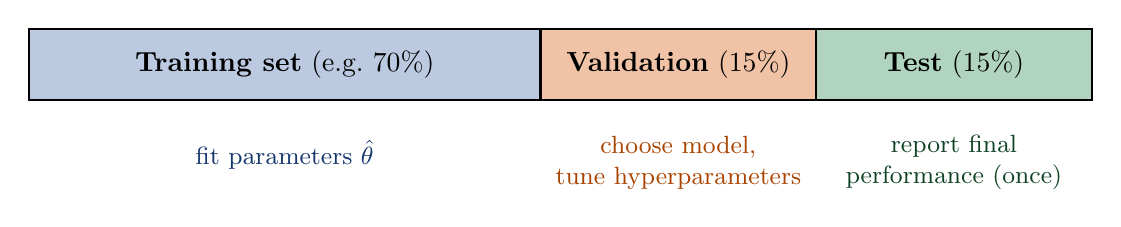
\begin{tikzpicture}
\fill[mlblue!30] (0,0) rectangle (6.5,0.9);
\fill[mlorange!35] (6.5,0) rectangle (10,0.9);
\fill[mlgreen!35] (10,0) rectangle (13.5,0.9);
\draw[thick] (0,0) rectangle (13.5,0.9);
\draw[thick] (6.5,0)--(6.5,0.9); \draw[thick] (10,0)--(10,0.9);
\node at (3.25,0.45) {\textbf{Training set} (e.g.\ 70\%)};
\node at (8.25,0.45) {\textbf{Validation} (15\%)};
\node at (11.75,0.45) {\textbf{Test} (15\%)};
\node[font=\small,mlblue!70!black,align=center] at (3.25,-0.7) {fit parameters $\hat\theta$};
\node[font=\small,mlorange!80!black,align=center] at (8.25,-0.8) {choose model,\\tune hyperparameters};
\node[font=\small,mlgreen!50!black,align=center] at (11.75,-0.8) {report final\\performance (once)};
\end{tikzpicture}
\caption{Splitting a dataset into training, validation and test sets.}\label{fig:split}
\end{figure}

\begin{explain}
The long bar is the \emph{whole} dataset, cut into three \textbf{non-overlapping} parts. The label under each part says its single job. The \textbf{blue} part is the only one the learning algorithm is allowed to fit. The \textbf{orange} part is used to \emph{compare} models and choose hyperparameters. The \textbf{green} part is kept locked away until the very end and used \emph{once} to report the final honest performance. Mixing these jobs (for example, tuning on the test part) makes the final number over-optimistic.
\end{explain}

%====================================================================
\section{Trade-offs in Statistical Learning}

\subsection{The Bias--Variance Trade-off}

Take a \emph{fixed} test point $x_0$. Imagine collecting many different training sets, each of size $n$, and fitting $\hat f$ on each one. The predictions $\hat f(x_0)$ vary from set to set. The expected squared prediction error at $x_0$ then splits into three parts:
\begin{equation}\label{eq:bv}
  \E\Big[\big(y_0-\hat f(x_0)\big)^2\Big]
  =\underbrace{\Big(\E[\hat f(x_0)]-f(x_0)\Big)^2}_{\Bias(\hat f(x_0))^2}
  +\underbrace{\E\Big[\big(\hat f(x_0)-\E[\hat f(x_0)]\big)^2\Big]}_{\Var(\hat f(x_0))}
  +\underbrace{\sigma^2}_{\text{irreducible}} .
\end{equation}

\begin{definition}[: Bias and variance of a method]
\textbf{Bias} is the error caused by approximating a complicated real problem by a simpler model: how far the \emph{average} prediction is from the truth. \textbf{Variance} is how much the prediction would \emph{change} if we trained on a different sample.
\end{definition}

\paragraph{Proof sketch of Equation~\eqref{eq:bv}.} Write $y_0=f+\varepsilon$ and let $\bar f=\E[\hat f]$. Add and subtract $\bar f$:
\[
  y_0-\hat f=(f-\bar f)+(\bar f-\hat f)+\varepsilon .
\]
Square and take expectations. The cross-terms vanish because $\E[\bar f-\hat f]=0$ and $\E[\varepsilon]=0$ with $\varepsilon$ independent of $\hat f$. What remains is $(f-\bar f)^2+\E[(\hat f-\bar f)^2]+\E[\varepsilon^2]$, i.e.\ $\Bias^2+\Var+\sigma^2$. $\qquad\blacksquare$

\begin{figure}[!htbp]
\centering
\tikzset{target/.pic={\fill[gray!12] (0,0) circle (1.2); \fill[gray!25] (0,0) circle (0.8);
  \fill[mlred!40] (0,0) circle (0.4); \draw[gray] (0,0) circle (1.2);}}
\resizebox{\linewidth}{!}{%
\begin{tikzpicture}
\foreach \x/\t in {0/{Low bias, low variance},3.4/{Low bias, high variance},6.8/{High bias, low variance},10.2/{High bias, high variance}}
  {\pic at (\x,0) {target}; \node[font=\small\bfseries,align=center,text width=3cm] at (\x,-1.9) {\t};}
\foreach \px/\py in {0.10/0.05,-0.10/0.12,0.05/-0.10,-0.08/-0.05,0.15/-0.02,-0.05/0.02}
  \fill[mlblue] (0+\px,\py) circle (0.06);
\foreach \px/\py in {0.7/0.5,-0.6/0.6,0.5/-0.7,-0.7/-0.4,0.1/0.9,-0.2/-0.9}
  \fill[mlblue] (3.4+\px,\py) circle (0.06);
\foreach \px/\py in {0.60/0.50,0.70/0.55,0.55/0.42,0.68/0.45,0.62/0.60,0.50/0.52}
  \fill[mlblue] (6.8+\px,\py) circle (0.06);
\foreach \px/\py in {0.9/0.7,0.3/0.9,1.0/0.0,0.6/0.3,-0.1/0.5,0.9/0.9}
  \fill[mlblue] (10.2+\px,\py) circle (0.06);
\end{tikzpicture}}
\caption{Bias and variance explained with a dartboard. Red centre = true value $f(x_0)$; blue dots = predictions from models trained on different samples.}\label{fig:darts}
\end{figure}

\begin{explain}
Think of each \textbf{blue dot} as the prediction made by a model trained on a different random sample, and the \textbf{red bull's-eye} as the true value.
\begin{itemize}
  \item \emph{Low bias, low variance:} dots are tightly clustered \emph{on} the centre. This is the ideal.
  \item \emph{Low bias, high variance:} dots are centred correctly on average but scattered. Predictions depend heavily on the particular sample (\textbf{overfitting}).
  \item \emph{High bias, low variance:} dots are tightly clustered but \emph{away} from the centre. The model is consistently wrong in the same way (\textbf{underfitting}).
  \item \emph{High bias, high variance:} dots are scattered and off-centre: the worst case.
\end{itemize}
\emph{Bias} is the distance from the \emph{centre of the dots} to the bull's-eye; \emph{variance} is the \emph{spread} of the dots.
\end{explain}

\begin{figure}[!htbp]
\centering
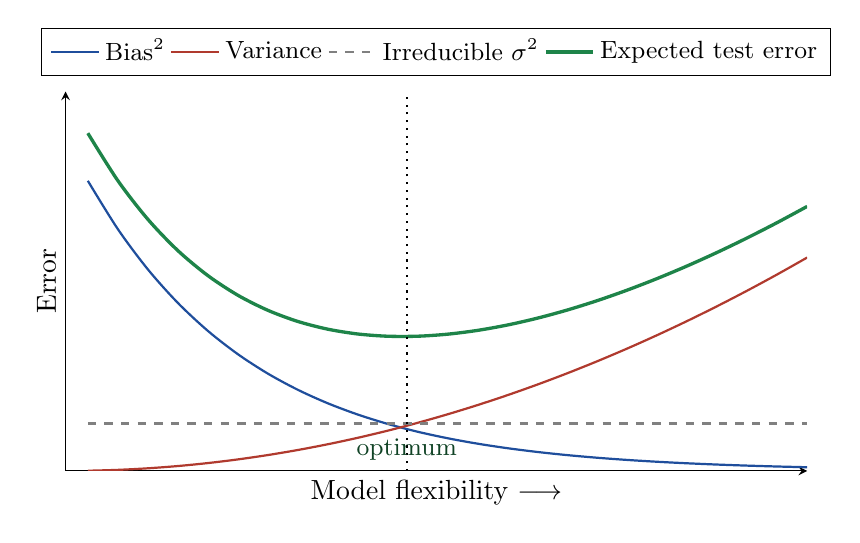
\begin{tikzpicture}
\begin{axis}[width=11cm,height=6.4cm,xlabel={Model flexibility $\longrightarrow$},ylabel={Error},
  xmin=0,xmax=10,ymin=0,ymax=8,ticks=none,axis lines=left,
  legend style={at={(0.5,1.04)},anchor=south,legend columns=4,font=\small}]
\addplot[thick,mlblue,smooth,domain=0.3:10]{7*exp(-0.45*x)};
\addplot[thick,mlred,smooth,domain=0.3:10]{0.045*x^2};
\addplot[thick,gray,dashed,domain=0.3:10]{1};
\addplot[very thick,mlgreen,smooth,domain=0.3:10]{7*exp(-0.45*x)+0.045*x^2+1};
\legend{Bias$^2$,Variance,Irreducible $\sigma^2$,Expected test error}
\draw[dotted,thick] (axis cs:4.6,0) -- (axis cs:4.6,8);
\node[font=\small,mlgreen!50!black] at (axis cs:4.6,0.45) {optimum};
\end{axis}
\end{tikzpicture}
\caption{Bias$^2$ falls and variance rises as flexibility increases; expected test error is their sum plus noise.}\label{fig:bvcurve}
\end{figure}

\begin{explain}
The horizontal axis is how flexible the model is (e.g.\ polynomial degree, or $1/k$ in k-NN). Read the four curves:
\begin{itemize}
  \item \textbf{Blue (bias$^2$)} starts high and falls: a flexible model can follow the true $f$ more closely.
  \item \textbf{Red (variance)} starts near zero and rises: a flexible model chases the noise in each training sample.
  \item \textbf{Grey dashed (irreducible error)} is a flat floor that no model can beat.
  \item \textbf{Green (expected test error)} is the \emph{sum} of the three. It is U-shaped: its lowest point (dotted line) is the best flexibility.
\end{itemize}
Left of the optimum, bias dominates (underfitting); right of it, variance dominates (overfitting). Compare this with Figure~\ref{fig:complexity} in Chapter~1.
\end{explain}

\begin{example}[: Putting numbers on the decomposition]
At a test point, a model has $\Bias^2=4$, $\Var=3$ and noise $\sigma^2=2$.
\[
  \text{Expected test MSE}=4+3+2=9 .
\]
If we switch to a more flexible model with $\Bias^2=1$ and $\Var=5$, the error becomes $1+5+2=8$: lower, even though variance rose, because the bias fell more. If flexibility is pushed further to $\Bias^2=0.5$, $\Var=9$, error is $0.5+9+2=11.5$: worse. This is the trade-off.
\end{example}

\begin{theory}{Bias--Variance Trade-off}
\tpart{Definition}
The expected squared prediction error at a point splits into three parts: $\E[(y_0-\hat f(x_0))^2]=\Bias^2+\Var+\sigma^2$. \textbf{Bias} is the error from simplifying assumptions; \textbf{variance} is the sensitivity of $\hat f$ to the particular training sample; $\sigma^2$ is irreducible noise. The \textbf{trade-off} is that lowering one usually raises the other.

\tpart{Explanation}
\begin{enumerate}[itemsep=2pt,topsep=3pt]
  \item Simple, inflexible model: \emph{high bias, low variance} $\Rightarrow$ underfitting.
  \item Complex, flexible model: \emph{low bias, high variance} $\Rightarrow$ overfitting.
  \item Test error is U-shaped in flexibility; the best model lies at the bottom.
\end{enumerate}

\tpart{How to control}
\begin{itemize}[itemsep=2pt,topsep=3pt]
  \item Choose flexibility with cross-validation
  \item Regularise to reduce variance
  \item Collect more data to reduce variance
  \item Ensemble methods (Chapter~5) reduce variance further
\end{itemize}

\tpart{Example}
With $\Bias^2=4$, $\Var=3$, $\sigma^2=2$ the expected test MSE is $9$; a more flexible model with $\Bias^2=1$, $\Var=5$ gives $8$ (better), while $\Bias^2=0.5$, $\Var=9$ gives $11.5$ (worse).

\end{theory}

\subsection{Other Trade-offs}

\begin{enumerate}
  \item \textbf{Flexibility vs.\ interpretability.} Simple models (linear regression) are easy to explain but may be too rigid; flexible models (boosting, deep networks) can fit complex patterns but act as black boxes.
  \item \textbf{Prediction accuracy vs.\ inference.} If you need to \emph{explain} effects, prefer simple models; if you only need accurate predictions, flexible models are fine.
  \item \textbf{Model complexity vs.\ amount of data.} Complex models need much more data. With little data, a simple model usually generalises better.
  \item \textbf{Training cost vs.\ accuracy.} More flexible models and more data take longer to train and need more memory.
\end{enumerate}

\begin{figure}[!htbp]
\centering
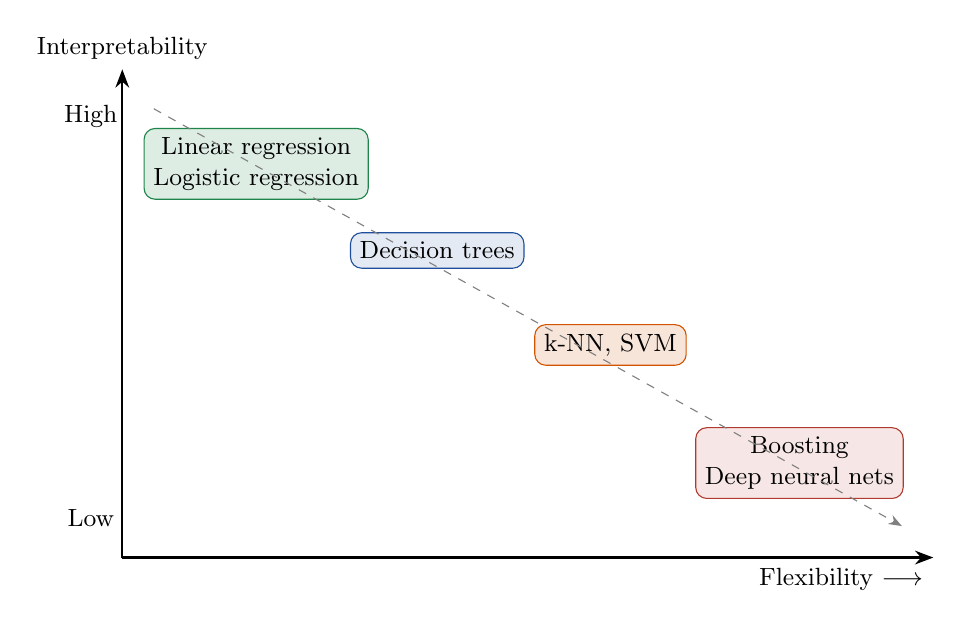
\begin{tikzpicture}
\draw[-{Stealth},thick] (0,0)--(10.3,0) node[below left,font=\small]{Flexibility $\longrightarrow$};
\draw[-{Stealth},thick] (0,0)--(0,6.2) node[above,font=\small]{Interpretability};
\node[font=\small] at (-0.4,5.6) {High}; \node[font=\small] at (-0.4,0.5) {Low};
\node[draw,rounded corners,fill=mlgreen!15,draw=mlgreen,font=\small,align=center] at (1.7,5.0) {Linear regression\\Logistic regression};
\node[draw,rounded corners,fill=mlblue!12,draw=mlblue,font=\small,align=center] at (4.0,3.9) {Decision trees};
\node[draw,rounded corners,fill=mlorange!15,draw=mlorange,font=\small,align=center] at (6.2,2.7) {k-NN, SVM};
\node[draw,rounded corners,fill=mlred!12,draw=mlred,font=\small,align=center] at (8.6,1.2) {Boosting\\Deep neural nets};
\draw[dashed,gray,-{Stealth}] (0.4,5.7)--(9.9,0.4);
\end{tikzpicture}
\caption{Typical position of methods on the flexibility--interpretability trade-off (qualitative).}\label{fig:flexinterp}
\end{figure}

\begin{explain}
Each box is a family of methods placed by two properties. Moving \textbf{right}, models become more flexible (can fit more complicated shapes). Moving \textbf{down}, they become harder to interpret. The dashed arrow shows the general trend: \emph{what you gain in flexibility you usually pay for in interpretability}. The positions are rough guides, not exact measurements; these methods are covered in Chapters~3--9.
\end{explain}

\begin{exam}
The bias--variance trade-off is the single most-asked topic of Unit~I. Be ready to (i)~state Equation~\eqref{eq:bv}, (ii)~sketch Figure~\ref{fig:bvcurve} with the four curves, and (iii)~link high bias to underfitting and high variance to overfitting.
\end{exam}

%====================================================================
\section{Estimating Risk Statistics}

We cannot compute the true risk $\Risk(\hat f)$, so we \emph{estimate} it. A good estimate should be nearly unbiased and have low variance.

\subsection{Hold-out (Validation-set) Estimate}

Split once into training and test parts and compute $\hat\Risk_{\text{test}}$. It is simple and fast, but (i)~the number depends on \emph{which} points fell in the test set, and (ii)~the model is trained on less data, so it may look slightly worse than it is.

\paragraph{Uncertainty of the estimate.} If the $m$ test losses $\ell_j=L(y'_j,\hat f(x'_j))$ have sample mean $\bar\ell=\hat\Risk_{\text{test}}$ and sample standard deviation $s$, then
\[
  \SE(\bar\ell)=\frac{s}{\sqrt m},\qquad
  \text{approximate 95\% CI for the risk: }\ \bar\ell\pm 1.96\,\SE(\bar\ell).
\]

\begin{example}[: Confidence interval for test MSE]
On $m=100$ test points the squared errors have mean $4.1$ and standard deviation $s=3$. Then
$\SE=3/\sqrt{100}=0.3$ and the 95\% interval is $4.1\pm1.96(0.3)=4.1\pm0.59$, i.e.\ $[3.51,\,4.69]$. So we may report ``test MSE $\approx 4.1$, likely between 3.5 and 4.7''. Quadrupling the test set to $m=400$ would halve the standard error to $0.15$.
\end{example}

\subsection{k-Fold Cross-Validation}

When data are scarce, we want to use \emph{all} of it for both training and evaluation.

\begin{figure}[!htbp]
\centering
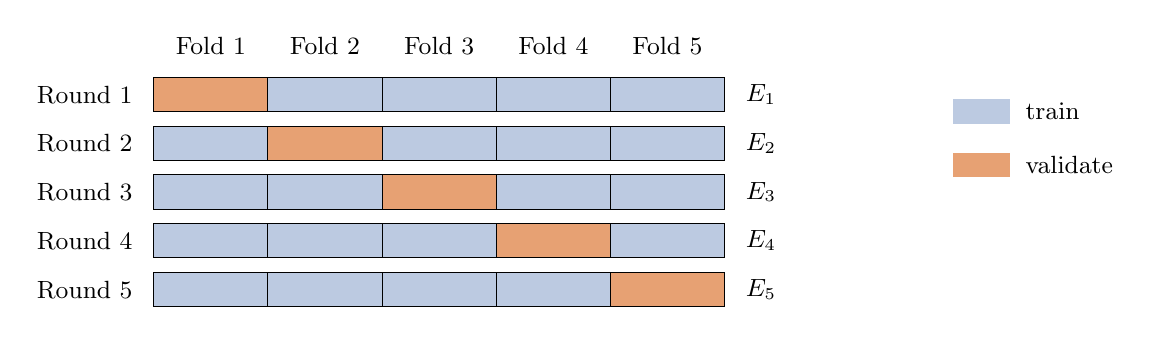
\begin{tikzpicture}[x=1.45cm,y=0.62cm]
\foreach \r in {1,...,5} {
  \node[left,font=\small] at (-0.1,-\r) {Round \r};
  \foreach \c in {1,...,5} {
    \ifnum\r=\c \fill[mlorange!55] (\c-1,-\r-0.35) rectangle (\c,-\r+0.35);
    \else \fill[mlblue!30] (\c-1,-\r-0.35) rectangle (\c,-\r+0.35); \fi
    \draw (\c-1,-\r-0.35) rectangle (\c,-\r+0.35);
  }
  \node[font=\small,right] at (5.1,-\r) {$E_{\r}$};
}
\foreach \c in {1,...,5} \node[font=\small] at (\c-0.5,0) {Fold \c};
\fill[mlblue!30] (7,-1.6) rectangle (7.5,-1.1); \node[right,font=\small] at (7.55,-1.35) {train};
\fill[mlorange!55] (7,-2.7) rectangle (7.5,-2.2); \node[right,font=\small] at (7.55,-2.45) {validate};
\end{tikzpicture}
\caption{5-fold cross-validation. Each round uses a different fold (orange) for validation and the other four (blue) for training.}\label{fig:kfold}
\end{figure}

\begin{explain}
The dataset is cut into $k=5$ equal \textbf{folds} (the columns). Each \textbf{row} is one training round. In Round~1 the model is trained on Folds 2--5 (blue) and its error $E_1$ is measured on Fold~1 (orange). In Round~2 the orange fold moves to Fold~2, and so on. After five rounds \emph{every point has been used for validation exactly once}, and the final estimate is the average $E_1,\dots,E_5$ of the five errors.
\end{explain}

\begin{definition}[: k-fold cross-validation estimate]
Split the data into $k$ folds. For $i=1,\dots,k$ train on all folds except the $i$-th and compute the error $E_i$ on the $i$-th. Then
\[
  \text{CV}_{(k)}=\frac1k\sum_{i=1}^{k}E_i .
\]
\end{definition}

\begin{example}[: 5-fold CV with numbers]
Validation errors: $E=(4.2,\ 3.8,\ 4.6,\ 4.0,\ 3.9)$.
\[
  \text{CV}_{(5)}=\frac{4.2+3.8+4.6+4.0+3.9}{5}=\frac{20.5}{5}=4.1 .
\]
Deviations from 4.1: $0.1,\,-0.3,\,0.5,\,-0.1,\,-0.2$; squares sum to $0.40$; $s^2=0.40/4=0.10$, $s=0.316$; $\SE=s/\sqrt5=0.141$. So the estimated risk is $4.1\pm0.14$.
\end{example}

\begin{theory}{k-fold Cross-Validation}
\tpart{Definition}
\textbf{k-fold cross-validation} estimates the risk of a model by splitting the data into $k$ equal folds, training on $k-1$ folds and validating on the remaining fold, repeating $k$ times, and averaging the $k$ validation errors.

\tpart{Working}
\begin{enumerate}[itemsep=2pt,topsep=3pt]
  \item Shuffle the data and split it into $k$ folds.
  \item For $i=1,\dots,k$: train on all folds except fold $i$; compute the error $E_i$ on fold $i$.
  \item Report $\mathrm{CV}_{(k)}=\frac1k\sum_iE_i$ (and its standard error).
\end{enumerate}

\tpart{Advantages}
\begin{itemize}[itemsep=2pt,topsep=3pt]
  \item Uses all data for both training and validation
  \item More reliable than a single hold-out split
  \item Standard tool for model selection and tuning
\end{itemize}

\tpart{Disadvantages}
\begin{itemize}[itemsep=2pt,topsep=3pt]
  \item Needs $k$ model fits, so it is $k$ times slower
  \item Not suitable as-is for time-series data (order matters)
\end{itemize}

\tpart{Applications}
\begin{itemize}[itemsep=2pt,topsep=3pt]
  \item Hyperparameter tuning
  \item Comparing different models
  \item Small datasets
\end{itemize}

\end{theory}

\paragraph{Choosing $k$.} \textbf{Leave-one-out CV (LOOCV)} is the extreme $k=n$: nearly unbiased but expensive and with high variance. In practice $k=5$ or $k=10$ gives a good bias--variance balance. For classification use \emph{stratified} folds, which keep the class proportions the same in each fold.

\begin{center}
\begin{tabular}{@{}p{3.1cm}p{3.5cm}p{3.5cm}p{3.5cm}@{}}
\toprule
 & \textbf{Hold-out} & \textbf{k-fold CV} & \textbf{LOOCV}\\
\midrule
Number of fits & 1 & $k$ & $n$\\
Computation & Cheapest & Moderate & Most expensive\\
Bias of estimate & Higher (less training data) & Low--moderate & Lowest\\
Variance of estimate & High (one split) & Moderate & High\\
Typical use & Large datasets & Default choice & Very small datasets\\
\bottomrule
\end{tabular}
\end{center}

\subsection{Risk Statistics for Classification}

For classification with 0--1 loss, the risk is the \textbf{error rate}. We summarise the test predictions in a \textbf{confusion matrix}.

\begin{center}
\begin{tabular}{@{}cc|cc@{}}
\toprule
 & & \multicolumn{2}{c}{\textbf{Predicted}}\\
 & & Positive & Negative\\
\midrule
\multirow{2}{*}{\textbf{Actual}} & Positive & TP (true positive) & FN (false negative)\\
 & Negative & FP (false positive) & TN (true negative)\\
\bottomrule
\end{tabular}
\end{center}

\[
\text{Accuracy}=\frac{TP+TN}{TP+TN+FP+FN},\quad
\text{Precision}=\frac{TP}{TP+FP},\quad
\text{Recall}=\frac{TP}{TP+FN},
\]
\[
\text{Specificity}=\frac{TN}{TN+FP},\qquad
F_1=\frac{2\cdot\text{Precision}\cdot\text{Recall}}{\text{Precision}+\text{Recall}} .
\]
\emph{Precision} answers ``of the items I flagged, how many were truly positive?''; \emph{recall} answers ``of all true positives, how many did I find?''; $F_1$ is their harmonic mean.

\begin{theory}{Confusion Matrix and Classification Metrics}
\tpart{Definition}
The \textbf{confusion matrix} tabulates a classifier's predictions against the true classes: true positives (TP), false negatives (FN), false positives (FP) and true negatives (TN). All classification metrics are computed from these four counts.

\tpart{Metrics}
\begin{itemize}[itemsep=2pt,topsep=3pt]
  \item \textbf{Accuracy} $=\frac{TP+TN}{TP+TN+FP+FN}$
  \item \textbf{Precision} $=\frac{TP}{TP+FP}$ (how many flagged items were correct)
  \item \textbf{Recall} $=\frac{TP}{TP+FN}$ (how many true positives were found)
  \item \textbf{$F_1$-score} $=\frac{2PR}{P+R}$ (harmonic mean of precision and recall)
\end{itemize}

\tpart{Advantages}
\begin{itemize}[itemsep=2pt,topsep=3pt]
  \item Shows \emph{what kind} of errors are made, not only how many
  \item Works for imbalanced data when precision/recall are used
\end{itemize}

\tpart{Disadvantages}
\begin{itemize}[itemsep=2pt,topsep=3pt]
  \item Accuracy misleads on imbalanced classes
  \item Depends on the chosen decision threshold
\end{itemize}

\tpart{Applications}
\begin{itemize}[itemsep=2pt,topsep=3pt]
  \item Medical screening, fraud detection, spam filtering
\end{itemize}

\end{theory}

\begin{example}[: Spam filter on 100 test e-mails]
Actual spam $=50$, actual non-spam $=50$. The filter finds $TP=40$ spam mails, misses $FN=10$, wrongly flags $FP=5$ good mails and correctly passes $TN=45$.
\begin{align*}
\text{Accuracy}&=\tfrac{40+45}{100}=0.85, & \text{Precision}&=\tfrac{40}{45}\approx0.889,\\
\text{Recall}&=\tfrac{40}{50}=0.80, & \text{Specificity}&=\tfrac{45}{50}=0.90,\\
F_1&=\tfrac{2(0.889)(0.80)}{0.889+0.80}\approx 0.842 . & &
\end{align*}
\end{example}

\begin{warning}
\textbf{Accuracy can mislead on imbalanced data.} If only 1\% of transactions are fraud, a program that always says ``not fraud'' is 99\% accurate yet has recall $0$ and is useless. Use precision, recall and $F_1$ instead.
\end{warning}

%====================================================================
\section{Sampling Distribution of an Estimator}

Everything we compute from data (a mean, a test error, a regression coefficient) is a \emph{statistic} calculated from a random sample. Draw a different sample and you get a different number. This section studies that randomness.

\begin{definition}[: Estimator and estimate]
An \textbf{estimator} $\hat\theta=g(X_1,\dots,X_n)$ is a \emph{rule} (a function of the sample) for guessing an unknown population quantity $\theta$. An \textbf{estimate} is the \emph{number} that the rule gives for one particular sample. Since the sample is random, the estimator $\hat\theta$ is itself a \textbf{random variable}.
\end{definition}

\begin{definition}[: Sampling distribution]
The \textbf{sampling distribution} of an estimator is its probability distribution over all possible samples of size $n$ from the population. Its \emph{standard deviation} is called the \textbf{standard error}, $\SE(\hat\theta)=\sqrt{\Var(\hat\theta)}$.
\end{definition}

\begin{theory}{Sampling Distribution of an Estimator}
\tpart{Definition}
An \textbf{estimator} $\hat\theta=g(X_1,\dots,X_n)$ is a rule for guessing a population quantity $\theta$ from a sample. Because the sample is random, $\hat\theta$ is a random variable; its probability distribution over all possible samples of size $n$ is its \textbf{sampling distribution}, and the standard deviation of that distribution is the \textbf{standard error} $\SE(\hat\theta)$.

\tpart{Working}
\begin{enumerate}[itemsep=2pt,topsep=3pt]
  \item Imagine drawing many samples of size $n$ from the population.
  \item Compute the statistic $\hat\theta$ for every sample.
  \item The spread of these values is the sampling distribution; its mean shows bias, its standard deviation gives the standard error.
\end{enumerate}

\tpart{Key properties}
\begin{itemize}[itemsep=2pt,topsep=3pt]
  \item \textbf{Unbiased:} $\E[\hat\theta]=\theta$
  \item \textbf{Low variance / standard error}: precise estimates
  \item \textbf{Consistent:} $\hat\theta\to\theta$ as $n\to\infty$
\end{itemize}

\tpart{Example}
For the sample mean, $\E[\bar X]=\mu$ and $\SE(\bar X)=\sigma/\sqrt n$; by the Central Limit Theorem $\bar X\approx\mathcal N(\mu,\sigma^2/n)$ for large $n$.

\tpart{Importance}
\begin{itemize}[itemsep=2pt,topsep=3pt]
  \item Gives confidence intervals: $\bar x\pm1.96\,\SE$
  \item Tells us how much to trust an estimate such as test error
\end{itemize}

\end{theory}

\subsection{Properties of Good Estimators}

\begin{center}
\begin{tabular}{@{}p{3.3cm}p{5.2cm}p{5cm}@{}}
\toprule
\textbf{Property} & \textbf{Definition} & \textbf{Meaning}\\
\midrule
Bias & $\Bias(\hat\theta)=\E[\hat\theta]-\theta$ & Average error; \textbf{unbiased} if $=0$\\
Variance & $\Var(\hat\theta)=\E[(\hat\theta-\E\hat\theta)^2]$ & Spread across samples\\
Standard error & $\SE(\hat\theta)=\sqrt{\Var(\hat\theta)}$ & Typical size of the estimation error\\
MSE & $\E[(\hat\theta-\theta)^2]=\Var(\hat\theta)+\Bias(\hat\theta)^2$ & Overall accuracy (same decomposition as before!)\\
Consistency & $\hat\theta\to\theta$ as $n\to\infty$ & More data gives a better estimate\\
\bottomrule
\end{tabular}
\end{center}

\subsection{The Sample Mean}

Let $X_1,\dots,X_n$ be i.i.d.\ with population mean $\mu$ and variance $\sigma^2$, and let $\bar X=\frac1n\sum X_i$. Then
\[
  \E[\bar X]=\mu\quad(\text{unbiased}),\qquad
  \Var(\bar X)=\frac{\sigma^2}{n},\qquad
  \SE(\bar X)=\frac{\sigma}{\sqrt n}.
\]
\emph{Proof.} $\E[\bar X]=\frac1n\sum\E[X_i]=\frac1n(n\mu)=\mu$, and, by independence, $\Var(\bar X)=\frac1{n^2}\sum\Var(X_i)=\frac{n\sigma^2}{n^2}=\frac{\sigma^2}{n}$. $\blacksquare$

\begin{keyidea}
The standard error shrinks like $1/\sqrt n$. To make an estimate \emph{twice} as precise you need \emph{four times} as much data.
\end{keyidea}

\begin{figure}[!htbp]
\centering
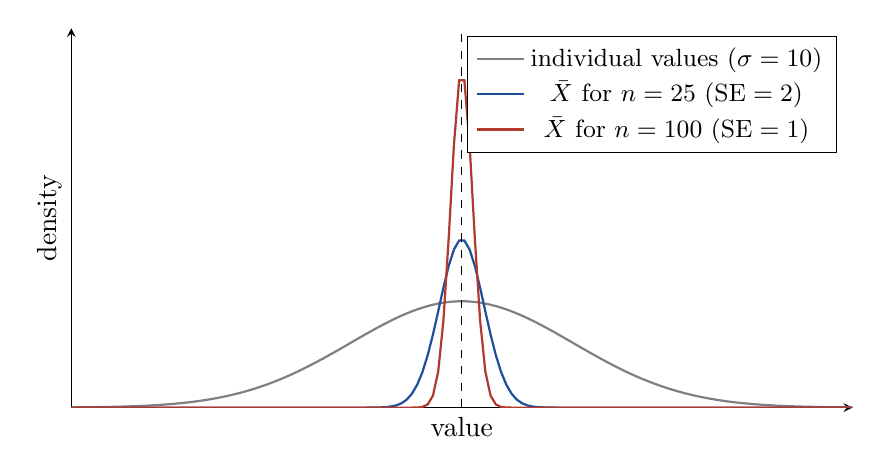
\begin{tikzpicture}
\begin{axis}[width=11.5cm,height=6.4cm,xlabel={value},ylabel={density},
  xmin=15,xmax=85,ymin=0,ymax=0.45,ticks=none,axis lines=left,samples=150,
  legend style={at={(0.98,0.98)},anchor=north east,font=\small}]
\addplot[thick,gray,domain=15:85]{1/(10*3.14159*2)^0.5*exp(-((x-50)^2)/(2*100))};
\addplot[thick,mlblue,domain=15:85]{1/(2*3.14159*4)^0.5*exp(-((x-50)^2)/(2*4))};
\addplot[thick,mlred,domain=15:85]{1/(2*3.14159*1)^0.5*exp(-((x-50)^2)/(2*1))};
\legend{individual values ($\sigma=10$),$\bar X$ for $n=25$ ($\SE=2$),$\bar X$ for $n=100$ ($\SE=1$)}
\draw[dashed] (axis cs:50,0) -- (axis cs:50,0.45);
\node[font=\small,anchor=north] at (axis cs:50,0) {$\mu=50$};
\end{axis}
\end{tikzpicture}
\caption{Sampling distribution of the sample mean for population mean $\mu=50$ and $\sigma=10$.}\label{fig:sampling}
\end{figure}

\begin{explain}
Three bell curves are drawn, all centred on the true mean $\mu=50$ (dashed line).
\begin{itemize}
  \item \textbf{Grey (widest):} the spread of \emph{individual} observations, $\sigma=10$.
  \item \textbf{Blue:} the distribution of the \emph{average of 25 observations}. It is still centred at 50 (\emph{unbiased}) but is $5\times$ narrower, $\SE=10/\sqrt{25}=2$.
  \item \textbf{Red (narrowest and tallest):} the average of 100 observations, $\SE=1$.
\end{itemize}
The \emph{height} of a curve at a value shows how likely it is that the estimate lands there. The bigger the sample, the more tightly the estimates cluster around the truth. Averages are much more reliable than single observations.
\end{explain}

\begin{example}[: Using the standard error]
A population has $\mu=50$ and $\sigma=10$. For samples of size $n=25$, what is $P(\bar X>53)$?\par
$\SE=10/\sqrt{25}=2$, so $z=\dfrac{53-50}{2}=1.5$ and $P(\bar X>53)=P(Z>1.5)\approx 0.0668$, about 6.7\%. With $n=100$, $\SE=1$, $z=3$, and the probability drops to about $0.0013$.
\end{example}

\subsection{Central Limit Theorem}

\begin{definition}[: Central Limit Theorem (CLT)]
Let $X_1,\dots,X_n$ be i.i.d.\ with mean $\mu$ and finite variance $\sigma^2$. For large $n$ the sampling distribution of $\bar X$ is approximately normal:
\[
  \bar X \;\approx\; \mathcal N\!\left(\mu,\ \frac{\sigma^2}{n}\right),\qquad\text{equivalently}\qquad
  \frac{\bar X-\mu}{\sigma/\sqrt n}\;\approx\; \mathcal N(0,1),
\]
\emph{whatever the shape of the original population}.
\end{definition}

The CLT is the reason the normal curve appears everywhere: test errors, accuracies and averages of many small effects are sums of many small random pieces. It justifies the confidence intervals used in the previous section (a rule of thumb: $n\ge 30$ is usually enough).

\paragraph{95\% confidence interval for a mean.} $\ \bar x \pm 1.96\,\dfrac{s}{\sqrt n}$.

\begin{example}[: Confidence interval]
A sample of $n=100$ gives $\bar x=52$ and $s=10$. $\SE=10/10=1$, so the 95\% interval is $52\pm1.96$, i.e.\ $[50.04,\,53.96]$. If we repeated the experiment many times, about 95\% of intervals built this way would contain the true $\mu$.
\end{example}

\subsection{A Biased Estimator: the Variance}

Not all natural estimators are unbiased. Consider estimating $\sigma^2$:
\[
  S_n^2=\frac1n\sum_{i=1}^n(X_i-\bar X)^2,\qquad
  S_{n-1}^2=\frac1{n-1}\sum_{i=1}^n(X_i-\bar X)^2 .
\]
It can be shown that $\E[S_n^2]=\dfrac{n-1}{n}\sigma^2<\sigma^2$, so $S_n^2$ is \textbf{biased} (it underestimates), while $S_{n-1}^2$ is unbiased. The reason is that deviations are measured from $\bar X$, which is itself fitted to the same data and so sits \emph{closer} to the sample than the true $\mu$ does. This is the same ``fits its own data too well'' effect that makes training loss optimistic.

\begin{example}[: Size of the bias]
With $n=5$ and $\sigma^2=10$: $\E[S_n^2]=\frac45(10)=8$ (bias $=-2$), whereas $\E[S_{n-1}^2]=10$.
\end{example}

\begin{tryit}
Verify the standard-error formula and the bias of $S_n^2$ by simulation:
\begin{lstlisting}
import numpy as np
rng = np.random.default_rng(1)

for n in [5, 25, 100]:
    means = [rng.normal(50, 10, n).mean() for _ in range(10000)]
    print(n, round(np.mean(means), 2), round(np.std(means), 2),
          round(10/np.sqrt(n), 2))      # theory: SE = sigma/sqrt(n)

v0 = [np.var(rng.normal(0, np.sqrt(10), 5), ddof=0) for _ in range(20000)]
v1 = [np.var(rng.normal(0, np.sqrt(10), 5), ddof=1) for _ in range(20000)]
print(round(np.mean(v0), 2), round(np.mean(v1), 2))
\end{lstlisting}
\textbf{Typical output:}
\begin{center}
\begin{tabular}{@{}cccc@{}}
\toprule
$n$ & mean of $\bar X$ & std of $\bar X$ & theory $10/\sqrt n$\\
\midrule
5 & 49.92 & 4.39 & 4.47\\
25 & 49.98 & 2.00 & 2.00\\
100 & 50.00 & 1.01 & 1.00\\
\bottomrule
\end{tabular}
\end{center}
The means stay near 50 (unbiased) and the spread follows $\sigma/\sqrt n$. The two variance estimates average about $8.0$ (ddof\,=\,0, biased) and $9.9$ (ddof\,=\,1, unbiased, close to the true 10).
\end{tryit}

\begin{keyidea}
Estimators (including a trained model's predictions and its test error) are random. To trust a number, we need to know \textbf{how much it would vary from sample to sample}: that is its \textbf{standard error}.
\end{keyidea}

%====================================================================
\begin{summary}
\begin{itemize}
  \item Statistical model: $Y=f(X)+\varepsilon$; we estimate $f$ for \emph{prediction} or \emph{inference}. Error = reducible + irreducible ($\sigma^2$).
  \item Supervised learning estimates $P(Y\mid X)$ (best predictors: conditional mean, Bayes classifier). Unsupervised learning studies $P(X)$.
  \item Loss measures a single mistake (squared, absolute, 0--1, cross-entropy); \textbf{risk} is expected loss; \textbf{training loss} (empirical risk) is optimistic; \textbf{test loss} is an honest estimate.
  \item $\E[(y_0-\hat f(x_0))^2]=\Bias^2+\Var+\sigma^2$. More flexibility lowers bias but raises variance; the best model balances them.
  \item Other trade-offs: flexibility vs.\ interpretability, prediction vs.\ inference, complexity vs.\ data size.
  \item Estimate risk by hold-out, k-fold CV ($k=5$ or $10$) or LOOCV; for classification use the confusion matrix, precision, recall and $F_1$.
  \item An estimator is a random variable; its spread is the \textbf{standard error}. For the sample mean $\SE=\sigma/\sqrt n$, and the \textbf{CLT} makes $\bar X$ approximately normal.
  \item $S_n^2$ (divide by $n$) is biased; $S_{n-1}^2$ is unbiased.
\end{itemize}
\end{summary}

%====================================================================
\section*{Exam Corner}
\addcontentsline{toc}{section}{Exam Corner}

\subsection*{A.\ Very Short Answer Questions (2 marks each)}
\begin{enumerate}
  \item Write the statistical model $Y=f(X)+\varepsilon$ and name each term. \qmarks{2}
  \item Differentiate between prediction and inference. \qmarks{2}
  \item What is irreducible error? \qmarks{2}
  \item Define a loss function. Give two examples. \qmarks{2}
  \item Why is training loss an optimistic estimate of the risk? \qmarks{2}
  \item Define bias and variance of a learning method. \qmarks{2}
  \item What is k-fold cross-validation? \qmarks{2}
  \item Define standard error of an estimator. \qmarks{2}
  \item State the Central Limit Theorem. \qmarks{2}
  \item Define precision and recall. \qmarks{2}
\end{enumerate}

\begin{modelans}[: Q5 and Q8]
\textbf{Q5.} The model parameters are chosen to \emph{minimise the loss on the training data itself}, so the model partly memorises its noise; on fresh data it performs worse. Hence training loss $\le$ expected test loss.\par
\textbf{Q8.} The standard error of an estimator $\hat\theta$ is the standard deviation of its sampling distribution, $\SE(\hat\theta)=\sqrt{\Var(\hat\theta)}$. For the sample mean it equals $\sigma/\sqrt n$.
\end{modelans}

\subsection*{B.\ Short Answer Questions (5 marks each)}
\begin{enumerate}
  \item Distinguish parametric and non-parametric methods with examples. \qmarks{5}
  \item Explain training loss, test loss and risk. Why do we need a separate test set? \qmarks{5}
  \item Explain the bias--variance trade-off with a diagram. \qmarks{5}
  \item Explain k-fold cross-validation with a diagram. Compare it with the hold-out method. \qmarks{5}
  \item Explain the confusion matrix and define accuracy, precision, recall and $F_1$. \qmarks{5}
  \item What is the sampling distribution of an estimator? Show that the sample mean is unbiased with $\Var(\bar X)=\sigma^2/n$. \qmarks{5}
  \item Why is accuracy a poor measure for imbalanced data? Illustrate with an example. \qmarks{5}
\end{enumerate}

\begin{modelans}[: B6 (outline for 5 marks)]
An \emph{estimator} $\hat\theta=g(X_1,\ldots,X_n)$ is a function of a random sample, hence a random variable; its probability distribution over repeated samples of size $n$ is its \emph{sampling distribution}.\par
For i.i.d.\ $X_i$ with mean $\mu$ and variance $\sigma^2$: $\E[\bar X]=\frac1n\sum\E[X_i]=\mu$, so $\bar X$ is unbiased. By independence, $\Var(\bar X)=\frac1{n^2}\sum\Var(X_i)=\frac{n\sigma^2}{n^2}=\frac{\sigma^2}{n}$. Hence $\SE(\bar X)=\sigma/\sqrt n$; precision improves as $n$ grows. By the CLT, $\bar X\approx\mathcal N(\mu,\sigma^2/n)$ for large $n$.
\end{modelans}

\subsection*{C.\ Long Answer Questions (10 marks each)}
\begin{enumerate}
  \item Derive the bias--variance decomposition of the expected squared prediction error. Explain its implications for model selection and sketch the curves. \qmarks{10}
  \item Describe the different methods of estimating the risk of a model (hold-out, k-fold, LOOCV) with their advantages and disadvantages. \qmarks{10}
  \item Explain the sampling distribution of the sample mean. State the CLT and explain, with an example, how it is used to construct a confidence interval. \qmarks{10}
  \item Compare supervised and unsupervised learning from a statistical point of view, and discuss the trade-offs in statistical learning. \qmarks{10}
  \item A classifier is tested on 200 samples: $TP=70$, $FN=30$, $FP=20$, $TN=80$. Compute accuracy, precision, recall, specificity and $F_1$. \qmarks{10}
\end{enumerate}

\begin{modelans}[: C5 (numerical)]
$n=200$. Accuracy $=\frac{70+80}{200}=0.75$. Precision $=\frac{70}{70+20}=0.778$. Recall $=\frac{70}{70+30}=0.70$. Specificity $=\frac{80}{80+20}=0.80$.\par
$F_1=\frac{2(0.778)(0.70)}{0.778+0.70}=\frac{1.089}{1.478}\approx\mathbf{0.737}$.
\end{modelans}

\subsection*{D.\ Numerical Problems}
\begin{enumerate}
  \item True $y=(2,4,6,8)$, predicted $\hat y=(3,3,6,10)$. Compute MAE, MSE and RMSE. \textit{(Answer: MAE $=1$, MSE $=1.5$, RMSE $=1.22$.)}
  \item A model has $\Bias^2=2.5$, $\Var=1.5$, $\sigma^2=1$. Find the expected test MSE. After switching to a simpler model, $\Bias^2=4$, $\Var=0.5$: which is better? \textit{(Answer: $5$; the new one gives $5.5$, so the first is better.)}
  \item 4-fold CV errors are $6,\,5,\,7,\,6$. Find the CV estimate and its standard error. \textit{(Answer: $6$; $s=0.816$, $\SE=0.408$.)}
  \item A population has $\mu=100$ and $\sigma=20$. For $n=64$, find $\SE(\bar X)$ and $P(\bar X<97)$. \textit{(Answer: $\SE=2.5$; $z=-1.2$; $P\approx0.115$.)}
  \item Test squared errors over 400 samples have mean $5$ and $s=4$. Give a 95\% CI for the risk. \textit{(Answer: $\SE=0.2$; $5\pm0.392=[4.61,5.39]$.)}
\end{enumerate}

\subsection*{E.\ Multiple-Choice Questions}
\begin{enumerate}
  \item The irreducible error in $Y=f(X)+\varepsilon$ is: \\
  (a) $\Bias^2$ \quad (b) $\Var(\hat f)$ \quad (c) $\Var(\varepsilon)$ \quad (d) $\hat\Risk_{\text{train}}$
  \item As model flexibility increases, typically: \\
  (a) bias$\uparrow$, variance$\downarrow$ \quad (b) bias$\downarrow$, variance$\uparrow$ \quad (c) both $\uparrow$ \quad (d) both $\downarrow$
  \item The best predictor under squared loss is: \\
  (a) the median of $Y$ \quad (b) the mode of $Y$ \quad (c) $\E[Y\mid X]$ \quad (d) $\E[Y]$
  \item In 10-fold CV, each observation is used for validation: \\
  (a) once \quad (b) ten times \quad (c) never \quad (d) a random number of times
  \item If $\sigma=12$ and $n=36$, then $\SE(\bar X)$ is: \\
  (a) 12 \quad (b) 6 \quad (c) 2 \quad (d) 0.33
  \item Which estimator of $\sigma^2$ is unbiased? \\
  (a) $\frac1n\sum(X_i-\bar X)^2$ \quad (b) $\frac1{n-1}\sum(X_i-\bar X)^2$ \quad (c) $\frac1{n+1}\sum(X_i-\bar X)^2$ \quad (d) none
  \item Recall is defined as: \\
  (a) $\frac{TP}{TP+FP}$ \quad (b) $\frac{TP}{TP+FN}$ \quad (c) $\frac{TN}{TN+FP}$ \quad (d) $\frac{TP+TN}{n}$
  \item Which loss is most robust to outliers? \\
  (a) squared \quad (b) absolute \quad (c) cubic \quad (d) exponential
\end{enumerate}
\textbf{Answers:} 1-c,\ 2-b,\ 3-c,\ 4-a,\ 5-c,\ 6-b,\ 7-b,\ 8-b.

\subsection*{F.\ Practice Problems}
\begin{enumerate}
  \item In Figure~\ref{fig:model}, suppose $f(x)=2x+1$ and $\sigma=0.5$. What is the smallest possible expected squared error for any model, and why?
  \item Run the polynomial experiment with degrees 2, 5 and 12 and sketch train/test MSE against degree. At which degree does the test MSE start rising?
  \item \textbf{Coding:} implement 5-fold cross-validation with \texttt{cross\_val\_score} for \texttt{LinearRegression} and report the mean and standard error of the scores.
  \item Simulate sampling distributions from a \emph{skewed} population (e.g.\ \texttt{rng.exponential(1, n)}) and verify with histograms that $\bar X$ becomes bell-shaped as $n$ grows (CLT).
\end{enumerate}

\begin{revision}
\begin{center}\small
\begin{tabular}{@{}p{3.6cm}p{9.6cm}@{}}
\toprule
\textbf{Topic} & \textbf{One-line recall}\\
\midrule
Model & $Y=f(X)+\varepsilon$, $\E\varepsilon=0$, $\Var\varepsilon=\sigma^2$.\\
Prediction / Inference & Accurate $\hat Y$ / understand effect of each $X_j$.\\
Error split & Reducible $+$ irreducible $\sigma^2$.\\
Best predictors & $\E[Y\mid X]$ (regression); Bayes classifier $\argmax_k P(k\mid x)$.\\
Risk & $\E[L(Y,f(X))]$ (unknown); train loss optimistic; test loss honest.\\
Bias--variance & $\E[(y_0-\hat f)^2]=\Bias^2+\Var+\sigma^2$; U-shaped test error.\\
Hold-out / k-fold / LOOCV & 1 fit / $k$ fits (use 5 or 10) / $n$ fits.\\
Classification stats & Acc $=\frac{TP+TN}{n}$, Prec $=\frac{TP}{TP+FP}$, Rec $=\frac{TP}{TP+FN}$, $F_1$ harmonic mean.\\
Sampling distribution & Distribution of an estimator over repeated samples; spread $=$ SE.\\
Sample mean & Unbiased; $\SE=\sigma/\sqrt n$; $4\times$ data $\Rightarrow$ $2\times$ precision.\\
CLT & $\bar X\approx\mathcal N(\mu,\sigma^2/n)$ for large $n$; 95\% CI $\bar x\pm1.96\SE$.\\
Variance estimator & Divide by $n-1$ for unbiasedness.\\
\bottomrule
\end{tabular}
\end{center}
\end{revision}

\chapter[Distance-Based Methods, Decision Trees and Naive Bayes]{Distance-Based Methods,\\Decision Trees and Naive Bayes}
\label{ch:knn}
\begin{objectives}
After studying this chapter you will be able to:
\begin{itemize}
  \item compute \textbf{Euclidean, Manhattan, Minkowski, Chebyshev, Hamming} and \textbf{cosine} measures and explain why \textbf{feature scaling} matters;
  \item apply the \textbf{k-Nearest Neighbours} algorithm to classification and regression, and explain the effect of $k$;
  \item build a \textbf{decision tree} by hand using \textbf{entropy, information gain} and \textbf{Gini index};
  \item explain \textbf{overfitting in trees} and \textbf{pruning};
  \item state \textbf{Bayes' theorem} and apply the \textbf{Naive Bayes} classifier, including \textbf{Laplace smoothing} and the \textbf{Gaussian} variant;
  \item compare the three methods and choose between them;
  \item answer 2-, 5- and 10-mark university questions on these topics.
\end{itemize}
\end{objectives}

\begin{pullquote}[--- Cover \& Hart, 1967 (on nearest neighbours)]
Birds of a feather flock together: the nearest neighbour of a point carries a lot of information about its class.
\end{pullquote}

This chapter begins Unit~II (Supervised Learning). The three methods here are among the simplest and most intuitive classifiers, and each uses a different idea:

\begin{center}
\begin{tabular}{@{}lll@{}}
\toprule
\textbf{Method} & \textbf{Core idea} & \textbf{Type (Chapter~1 / 2)}\\
\midrule
k-Nearest Neighbours & ``You are like your closest neighbours'' & instance-based, non-parametric\\
Decision tree & ``Ask a sequence of yes/no questions'' & model-based, non-parametric\\
Naive Bayes & ``Use probability and Bayes' rule'' & model-based, parametric\\
\bottomrule
\end{tabular}
\end{center}

%====================================================================
\section{Distance-Based Methods}

Many learning algorithms (k-NN, K-Means, SVMs with kernels) depend on one question: \emph{how similar are two instances?} We answer it with a \textbf{distance} (small = similar) or a \textbf{similarity} (large = similar).

\begin{definition}[: Distance-based methods]
\textbf{Distance-based methods} make predictions or form groups using the \emph{distance (or similarity) between instances} in feature space: close points are assumed to be similar.
\end{definition}

\begin{definition}[: Distance metric]
A function $d(\vect{a},\vect{b})$ is a \textbf{metric} if for all points: (i)~$d(\vect{a},\vect{b})\ge0$ and $d(\vect{a},\vect{b})=0\iff\vect{a}=\vect{b}$; (ii)~symmetry $d(\vect{a},\vect{b})=d(\vect{b},\vect{a})$; (iii)~triangle inequality $d(\vect{a},\vect{c})\le d(\vect{a},\vect{b})+d(\vect{b},\vect{c})$.
\end{definition}

\subsection{Common Distance Measures}

For two $d$-dimensional points $\vect{a}=(a_1,\dots,a_d)$ and $\vect{b}=(b_1,\dots,b_d)$:

\begin{center}
\begin{tabular}{@{}p{3.3cm}p{5.8cm}p{4.4cm}@{}}
\toprule
\textbf{Measure} & \textbf{Formula} & \textbf{Use}\\
\midrule
Euclidean ($L_2$) & $\sqrt{\sum_i (a_i-b_i)^2}$ & Default for numeric data\\
Manhattan ($L_1$) & $\sum_i |a_i-b_i|$ & Grid-like paths; less sensitive to outliers\\
Minkowski ($L_p$) & $\big(\sum_i |a_i-b_i|^p\big)^{1/p}$ & General family ($p=1,2$ above)\\
Chebyshev ($L_\infty$) & $\max_i |a_i-b_i|$ & Largest single difference\\
Hamming & number of positions where $a_i\neq b_i$ & Binary / categorical strings\\
Cosine similarity & $\dfrac{\vect{a}\cdot\vect{b}}{\|\vect{a}\|\,\|\vect{b}\|}$ & Text; direction, not size\\
\bottomrule
\end{tabular}
\end{center}

\begin{example}[: Computing distances]
Let $\vect{a}=(1,2,3)$ and $\vect{b}=(4,6,3)$. The coordinate differences are $3,4,0$.
\begin{align*}
d_{L_2}&=\sqrt{3^2+4^2+0^2}=\sqrt{25}=5, &
d_{L_1}&=3+4+0=7,\\
d_{L_\infty}&=\max(3,4,0)=4, &
d_{L_3}&=(27+64+0)^{1/3}=91^{1/3}\approx4.50.
\end{align*}
Cosine similarity: $\vect{a}\cdot\vect{b}=4+12+9=25$, $\|\vect{a}\|=\sqrt{14}\approx3.742$, $\|\vect{b}\|=\sqrt{61}\approx7.810$, so $\cos\theta=25/29.22\approx0.855$.\par
Hamming: for the bit strings $10110$ and $11100$ the strings differ in positions 2 and 4, so $d_H=2$.\par
\textbf{Note the ordering} $L_\infty\le L_3\le L_2\le L_1$ for the same pair of points.
\end{example}

\begin{figure}[!htbp]
\centering
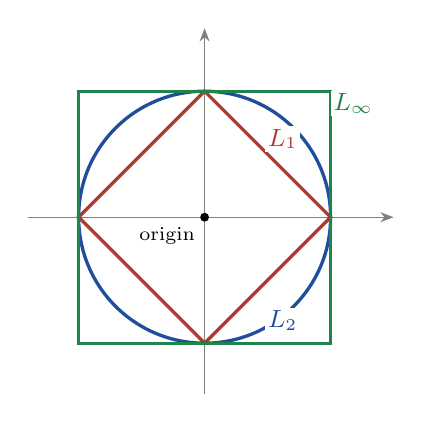
\begin{tikzpicture}[scale=1.6]
\draw[-{Stealth},gray] (-1.4,0)--(1.5,0); \draw[-{Stealth},gray] (0,-1.4)--(0,1.5);
\draw[very thick,mlred] (1,0)--(0,1)--(-1,0)--(0,-1)--cycle;
\draw[very thick,mlblue] (0,0) circle (1);
\draw[very thick,mlgreen] (-1,-1) rectangle (1,1);
\node[mlred,font=\small,fill=white,inner sep=1pt] at (0.62,0.62) {$L_1$};
\node[mlblue,font=\small,fill=white,inner sep=1pt] at (0.62,-0.82) {$L_2$};
\node[mlgreen,font=\small,fill=white,inner sep=1pt] at (1.18,0.9) {$L_\infty$};
\fill (0,0) circle (1pt) node[below left,font=\scriptsize] {origin};
\end{tikzpicture}
\caption{The set of all points at distance exactly 1 from the origin, for three metrics.}\label{fig:unitballs}
\end{figure}

\begin{explain}
Each coloured outline is the set of points that are \emph{exactly one unit away} from the origin under a different distance. Under \textbf{Euclidean} distance ($L_2$, blue) this set is a \emph{circle}. Under \textbf{Manhattan} ($L_1$, red) it is a \emph{diamond}, because you may only move along the axes. Under \textbf{Chebyshev} ($L_\infty$, green) it is a \emph{square}. The point $(1,1)$ lies on the green square but far outside the red diamond: the \emph{same pair of points} is counted as ``close'' or ``far'' depending on the metric. Hence the choice of metric changes which points are neighbours.
\end{explain}


\subsection{Feature Scaling}

Distance measures add up differences across all features, so a feature with a \emph{large numeric range} dominates the sum. We must put features on a comparable scale.

\begin{center}
\begin{tabular}{@{}p{3.6cm}p{5cm}p{4.6cm}@{}}
\toprule
\textbf{Method} & \textbf{Formula} & \textbf{Result}\\
\midrule
Min--max scaling & $x'=\dfrac{x-x_{\min}}{x_{\max}-x_{\min}}$ & Values in $[0,1]$\\[3mm]
Standardisation (z-score) & $x'=\dfrac{x-\mu}{\sigma}$ & Mean 0, standard deviation 1\\
\bottomrule
\end{tabular}
\end{center}

\begin{example}[: Why scaling matters]
Three people: $P=(\text{age }25,\ \text{salary }40000)$, $Q=(45,\ 42000)$, $R=(26,\ 80000)$. Raw Euclidean distances:
\[
d(P,Q)=\sqrt{20^2+2000^2}\approx2000.1,\qquad d(P,R)=\sqrt{1^2+40000^2}\approx40000.0 .
\]
The salary difference swamps age, so $Q$ (20 years older) looks far closer to $P$ than $R$ (1 year older) does, which is silly. Now min--max scale with age range $20$--$60$ and salary range $20\,000$--$100\,000$:
\[
P'=(0.125,\,0.250),\quad Q'=(0.625,\,0.275),\quad R'=(0.150,\,0.750).
\]
$d(P',Q')=\sqrt{0.5^2+0.025^2}\approx0.5006$ and $d(P',R')=\sqrt{0.025^2+0.5^2}\approx0.5006$: after scaling, age and salary contribute fairly.
\end{example}

\begin{warning}
Always compute the scaling parameters ($x_{\min},x_{\max},\mu,\sigma$) on the \textbf{training set only} and then apply the \emph{same} numbers to the test set. Using the test data to compute them leaks information.
\end{warning}

%====================================================================
\procon{Distance-based methods}
{\item Intuitive and easy to implement
 \item Little or no training
 \item Works for classification, regression and clustering}
{\item Very sensitive to feature scale and irrelevant features
 \item Slow for large datasets
 \item Loses meaning in high dimensions (curse of dimensionality)}
{\item k-NN and K-Means clustering
 \item Recommender systems
 \item Anomaly detection}

\section{Nearest Neighbours (k-NN)}

\subsection{The Algorithm}

k-NN is the simplest learning algorithm: it has \textbf{no training phase}. It just stores the training data (a \emph{lazy learner}) and does all the work at prediction time.

\begin{definition}[: k-Nearest Neighbours]
To predict for a new point $\vect{x}_q$:
\begin{enumerate}
  \item Compute the distance from $\vect{x}_q$ to every training point.
  \item Pick the $k$ training points with the smallest distances (the \emph{neighbourhood} $N_k(\vect{x}_q)$).
  \item \textbf{Classification:} output the \emph{majority class} among the $k$ neighbours.\\
        \textbf{Regression:} output the \emph{mean} of their target values.
\end{enumerate}
\end{definition}

\begin{example}[: k-NN classification by hand]
Training data (two features, two classes) and the query $\vect{x}_q=(5,4)$:

\begin{center}
\begin{tabular}{@{}c|cc|c|c|c@{}}
\toprule
Point & $x_1$ & $x_2$ & Class & Distance to $(5,4)$ & Rank\\
\midrule
$P_4$ & 6 & 5 & B & $\sqrt{1+1}=1.414$ & 1\\
$P_5$ & 7 & 4 & B & $\sqrt{4+0}=2.000$ & 2--3\\
$P_6$ & 5 & 6 & B & $\sqrt{0+4}=2.000$ & 2--3\\
$P_7$ & 4 & 2 & A & $\sqrt{1+4}=2.236$ & 4\\
$P_3$ & 3 & 2 & A & $\sqrt{4+4}=2.828$ & 5\\
$P_2$ & 2 & 3 & A & $\sqrt{9+1}=3.162$ & 6\\
$P_1$ & 1 & 1 & A & $\sqrt{16+9}=5.000$ & 7\\
\bottomrule
\end{tabular}
\end{center}

\begin{center}
\begin{tabular}{@{}cll@{}}
\toprule
$k$ & Neighbours & Prediction\\
\midrule
1 & $P_4$ (B) & \textbf{B}\\
3 & $P_4,P_5,P_6$ = B,B,B & \textbf{B}\\
5 & B,B,B,A,A (3 vs 2) & \textbf{B}\\
7 & all points: 4 A vs 3 B & \textbf{A}\\
\bottomrule
\end{tabular}
\end{center}
The prediction \emph{changes} from B to A when $k$ grows to 7, which shows how sensitive k-NN is to $k$.
\end{example}

\begin{figure}[!htbp]
\centering
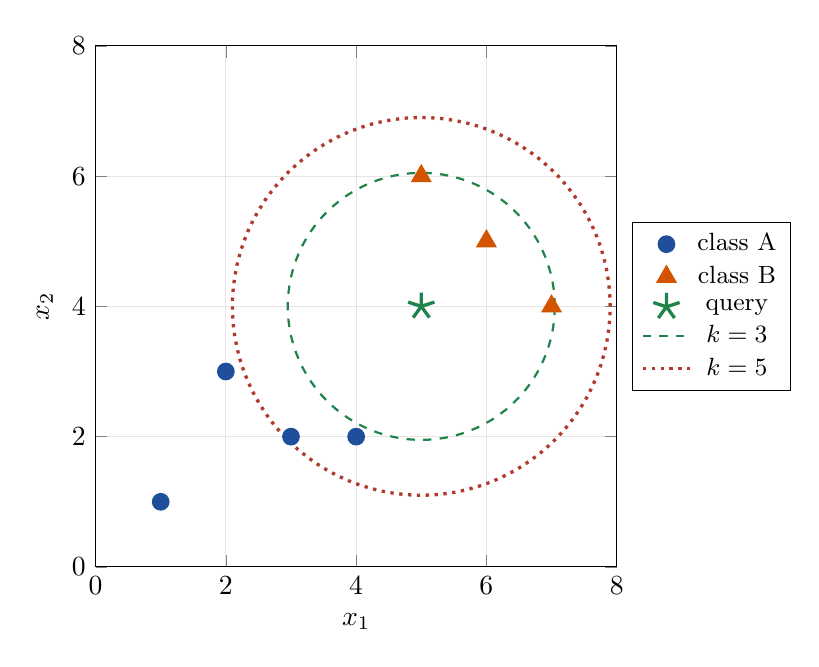
\begin{tikzpicture}
\begin{axis}[width=8.2cm,height=8.2cm,xmin=0,xmax=8,ymin=0,ymax=8,xlabel={$x_1$},ylabel={$x_2$},
  axis equal image,grid=both,grid style={gray!20},legend style={at={(1.03,0.5)},anchor=west,font=\small}]
\addplot[only marks,mark=*,mlblue,mark size=3pt] coordinates {(1,1)(2,3)(3,2)(4,2)};
\addlegendentry{class A}
\addplot[only marks,mark=triangle*,mlorange,mark size=4pt] coordinates {(6,5)(7,4)(5,6)};
\addlegendentry{class B}
\addplot[only marks,mark=star,mlgreen,mark size=5pt,very thick] coordinates {(5,4)};
\addlegendentry{query}
\addplot[dashed,mlgreen,thick,domain=0:360,samples=100,variable=\t]({5+2.05*cos(t)},{4+2.05*sin(t)});
\addlegendentry{$k=3$}
\addplot[dotted,mlred,very thick,domain=0:360,samples=100,variable=\t]({5+2.9*cos(t)},{4+2.9*sin(t)});
\addlegendentry{$k=5$}
\end{axis}
\end{tikzpicture}
\caption{Neighbourhoods of the query point for $k=3$ and $k=5$.}\label{fig:knn}
\end{figure}

\begin{explain}
The \textbf{green star} is the query point. Blue circles are class~A and orange triangles are class~B. The \textbf{dashed green circle} is just big enough to contain the 3 nearest points: all three are orange, so $k=3$ votes B. The \textbf{dotted red circle} is large enough to contain 5 points: three orange and two blue, so $k=5$ still votes B, but by a smaller margin. If we kept enlarging the circle to include all 7 points the blue majority would win. The \emph{radius adapts} to the local density of data; this is why k-NN is called \emph{local}.
\end{explain}


\subsection{Choosing $k$}

\begin{center}
\begin{tabular}{@{}p{2.8cm}p{5.5cm}p{5.5cm}@{}}
\toprule
 & \textbf{Small $k$ (e.g.\ 1)} & \textbf{Large $k$}\\
\midrule
Decision boundary & Very jagged, follows every point & Smooth\\
Bias & Low & High\\
Variance & High (sensitive to noise) & Low\\
Risk & Overfitting & Underfitting\\
\bottomrule
\end{tabular}
\end{center}

$k$ is a \textbf{hyperparameter}, chosen by cross-validation (Chapter~2). Use an \emph{odd} $k$ for two-class problems to avoid ties. A common starting point is $k\approx\sqrt n$.

\begin{keyidea}
$1/k$ is a measure of model flexibility: $k=1$ is the \emph{most flexible} (and most variable) k-NN; $k=n$ always predicts the overall majority class (the least flexible). This is the bias--variance trade-off of Chapter~2 in action.
\end{keyidea}

\subsection{Weighted k-NN and k-NN Regression}

In \textbf{weighted k-NN}, closer neighbours get more influence, with a weight $w_i=1/d_i$ (or $1/d_i^2$).

\begin{example}[: k-NN regression]
Use the house data of Chapter~1: size $x=1,2,3,4,5$ with price $y=15,26,29,44,46$. Predict the price at $x_q=3.4$ with $k=2$. The two nearest sizes are $x=3$ (distance $0.4$, price $29$) and $x=4$ (distance $0.6$, price $44$).
\begin{itemize}
  \item \textbf{Plain average:} $\hat y=(29+44)/2=36.5$.
  \item \textbf{Weighted ($w=1/d$):} $w_1=2.5$, $w_2=1.667$; $\hat y=\dfrac{2.5(29)+1.667(44)}{2.5+1.667}=\dfrac{145.83}{4.167}=35.0$.
\end{itemize}
The weighted answer is pulled towards the closer house (price 29). For comparison, the linear model $8+8x$ from Chapter~1 predicts $35.2$.
\end{example}

\subsection{Strengths and Weaknesses}

\begin{center}
\begin{tabular}{@{}p{6.7cm}p{6.7cm}@{}}
\toprule
\textbf{Advantages} & \textbf{Disadvantages}\\
\midrule
Very simple; no training & Slow prediction: must scan all $n$ points ($O(nd)$ per query)\\
Naturally handles multiple classes & Needs a lot of memory (stores everything)\\
No assumption about the data shape & Sensitive to feature scale and irrelevant features\\
Improves as more data arrives & Suffers from the \emph{curse of dimensionality}\\
\bottomrule
\end{tabular}
\end{center}

\paragraph{Curse of dimensionality.} In high dimensions, points become almost equally far apart, so the idea of a ``nearest'' neighbour loses meaning and k-NN degrades. Remedies: feature selection and dimensionality reduction such as PCA (Chapter~8).

%====================================================================
\procon{k-Nearest neighbours (k-NN)}
{\item Simple; no training; handles many classes
 \item No assumption about the data distribution
 \item Improves as more data is added}
{\item Slow prediction and large memory
 \item Sensitive to $k$, scaling and irrelevant features
 \item Poor in high dimensions}
{\item Recommendation systems
 \item Handwriting and pattern recognition
 \item Credit rating and anomaly detection}

\section{Decision Trees}

\subsection{Idea and Structure}

A decision tree predicts by asking a sequence of simple questions about the features, like a game of ``twenty questions''.

\begin{definition}[: Decision tree]
A \textbf{decision tree} is a flowchart-like model in which each \textbf{internal node} tests one feature, each \textbf{branch} is an outcome of the test, and each \textbf{leaf} holds a prediction (a class label for \emph{classification trees}, or a number for \emph{regression trees}). The top node is the \textbf{root}.
\end{definition}

The learning problem is: \emph{which feature should we test at each node?} We choose the test that makes the resulting groups as \textbf{pure} as possible, i.e.\ each group dominated by one class.

\subsection{Measures of Impurity}

Let a node contain examples of $C$ classes with proportions $p_1,\dots,p_C$.

\begin{definition}[: Entropy]
\[
  H=-\sum_{i=1}^{C}p_i\log_2 p_i\qquad(0\log0:=0).
\]
Entropy is $0$ when the node is pure and is maximal ($\log_2C$) when all classes are equally likely. It is measured in \emph{bits}.
\end{definition}

\begin{definition}[: Gini index]
\[
  G=1-\sum_{i=1}^{C}p_i^2 .
\]
Gini is $0$ for a pure node and equals $0.5$ for a 50/50 two-class node. It is the probability that two items drawn at random from the node have different classes.
\end{definition}

\begin{figure}[!htbp]
\centering
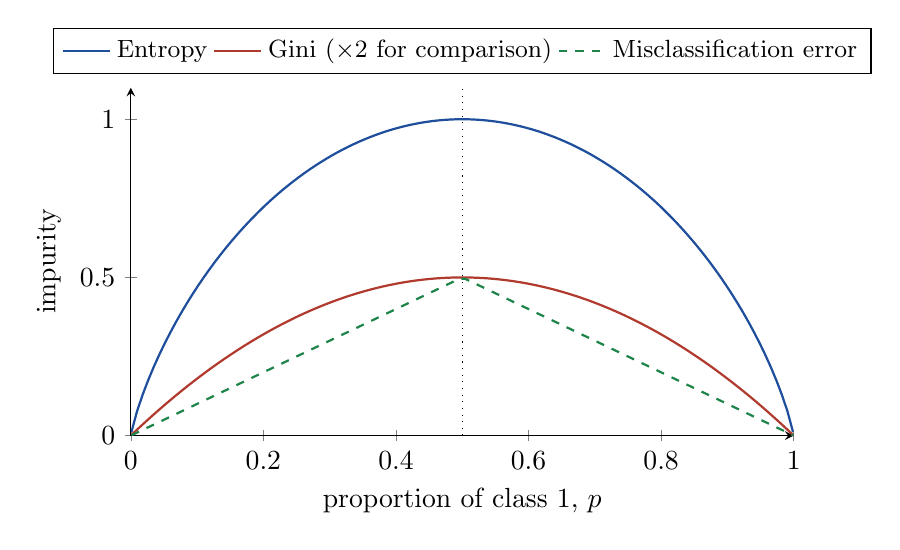
\begin{tikzpicture}
\begin{axis}[width=10cm,height=6cm,xlabel={proportion of class 1, $p$},ylabel={impurity},
  xmin=0,xmax=1,ymin=0,ymax=1.1,domain=0.001:0.999,samples=120,axis lines=left,
  legend style={at={(0.5,1.04)},anchor=south,legend columns=3,font=\small}]
\addplot[thick,mlblue]{-x*ln(x)/ln(2)-(1-x)*ln(1-x)/ln(2)};
\addplot[thick,mlred]{2*x*(1-x)};
\addplot[thick,mlgreen,dashed]{1-max(x,1-x)};
\legend{Entropy,Gini ($\times2$ for comparison),Misclassification error}
\draw[dotted] (axis cs:0.5,0)--(axis cs:0.5,1.1);
\end{axis}
\end{tikzpicture}
\caption{Impurity measures for a two-class node as a function of $p$.}\label{fig:impurity}
\end{figure}

\begin{explain}
The horizontal axis is the \textbf{proportion of class 1} in a node: $p=0$ or $p=1$ means a \emph{pure} node and $p=0.5$ is the most mixed. All three curves are \textbf{zero at the ends} (pure) and \textbf{highest at the middle} (maximum confusion). \textbf{Entropy} (blue) is slightly more curved than \textbf{Gini} (red; drawn here as $2p(1-p)$ so that it peaks at 1 like entropy). In practice they almost always choose the same splits. The dashed green \emph{misclassification error} has a sharp corner and is less sensitive to changes, which is why it is rarely used for growing trees.
\end{explain}

\begin{definition}[: Information gain]
If a split on feature $A$ divides a set $S$ into subsets $S_v$ (one for each value $v$ of $A$), then
\[
  \text{Gain}(S,A)=H(S)-\sum_{v}\frac{|S_v|}{|S|}\,H(S_v).
\]
It is the \emph{reduction in entropy} achieved by the split. At each node the tree picks the feature with the \textbf{highest information gain}. (The ID3 algorithm does exactly this; C4.5 uses the \emph{gain ratio} to avoid favouring features with many values; CART uses the Gini index and binary splits.)
\end{definition}

\subsection{Worked Example: Building a Tree with ID3}

We want to decide whether to \textbf{play tennis} from the weather. There are 14 past days.

\begin{center}
\small
\begin{tabular}{@{}cllllc@{}}
\toprule
\textbf{Day} & \textbf{Outlook} & \textbf{Temp.} & \textbf{Humidity} & \textbf{Wind} & \textbf{Play}\\
\midrule
D1 & Sunny & Hot & High & Weak & No\\
D2 & Sunny & Hot & High & Strong & No\\
D3 & Overcast & Hot & High & Weak & Yes\\
D4 & Rain & Mild & High & Weak & Yes\\
D5 & Rain & Cool & Normal & Weak & Yes\\
D6 & Rain & Cool & Normal & Strong & No\\
D7 & Overcast & Cool & Normal & Strong & Yes\\
D8 & Sunny & Mild & High & Weak & No\\
D9 & Sunny & Cool & Normal & Weak & Yes\\
D10 & Rain & Mild & Normal & Weak & Yes\\
D11 & Sunny & Mild & Normal & Strong & Yes\\
D12 & Overcast & Mild & High & Strong & Yes\\
D13 & Overcast & Hot & Normal & Weak & Yes\\
D14 & Rain & Mild & High & Strong & No\\
\bottomrule
\end{tabular}
\end{center}

\paragraph{Step 1: entropy of the whole set.} There are 9 Yes and 5 No:
\[
H(S)=-\tfrac{9}{14}\log_2\tfrac{9}{14}-\tfrac{5}{14}\log_2\tfrac{5}{14}=0.410+0.530=\mathbf{0.940}.
\]

\paragraph{Step 2: information gain of every feature.}

\begin{center}
\begin{tabular}{@{}lccc@{}}
\toprule
\textbf{Split} & \textbf{Values (Yes, No)} & \textbf{Entropies} & \textbf{Gain}\\
\midrule
Outlook & Sunny (2,3), Overcast (4,0), Rain (3,2) & $0.971,\ 0,\ 0.971$ & $\mathbf{0.247}$\\
Humidity & High (3,4), Normal (6,1) & $0.985,\ 0.592$ & $0.152$\\
Wind & Weak (6,2), Strong (3,3) & $0.811,\ 1.000$ & $0.048$\\
Temperature & Hot (2,2), Mild (4,2), Cool (3,1) & $1.000,\ 0.918,\ 0.811$ & $0.029$\\
\bottomrule
\end{tabular}
\end{center}

\emph{Detail for Outlook:}
\[
\text{Gain}=0.940-\tfrac{5}{14}(0.971)-\tfrac{4}{14}(0)-\tfrac{5}{14}(0.971)=0.940-0.694=0.247 .
\]
\textbf{Outlook has the highest gain, so it becomes the root.}

\paragraph{Step 3: recurse on each branch.}
\begin{itemize}
  \item \textbf{Overcast:} all 4 days are Yes $\Rightarrow$ pure $\Rightarrow$ leaf \emph{Yes}.
  \item \textbf{Sunny} (D1, D2, D8, D9, D11; 2 Yes, 3 No): splitting on Humidity gives High $\to$ \{D1, D2, D8\} all No, Normal $\to$ \{D9, D11\} all Yes. Both pure, so Humidity is chosen.
  \item \textbf{Rain} (D4, D5, D6, D10, D14; 3 Yes, 2 No): splitting on Wind gives Weak $\to$ \{D4, D5, D10\} all Yes, Strong $\to$ \{D6, D14\} all No.
\end{itemize}

\begin{figure}[!htbp]
\centering
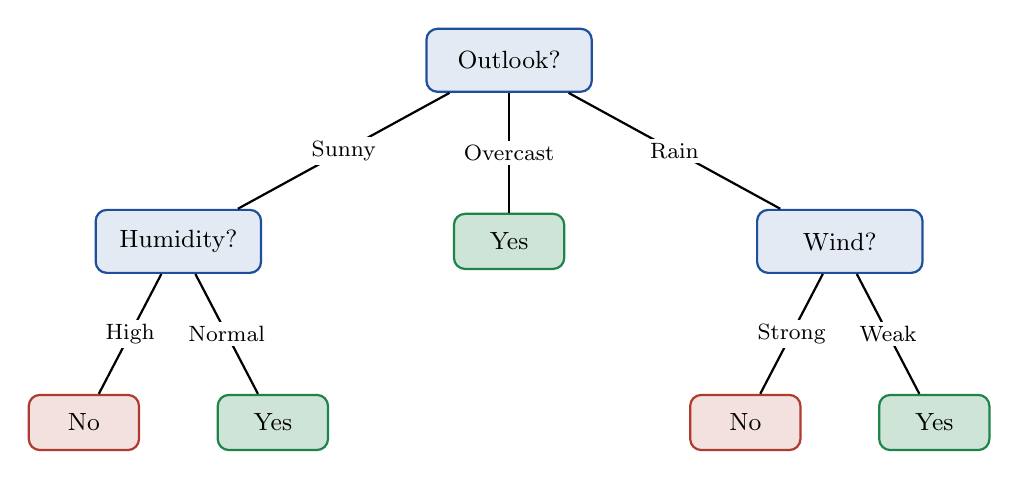
\begin{tikzpicture}[
  every node/.style={font=\small},
  dec/.style={draw,rounded corners,fill=mlblue!12,draw=mlblue,thick,minimum width=2.1cm,minimum height=0.8cm},
  yes/.style={draw,fill=mlgreen!22,draw=mlgreen,thick,minimum width=1.4cm,minimum height=0.7cm,rounded corners},
  no/.style={draw,fill=mlred!15,draw=mlred,thick,minimum width=1.4cm,minimum height=0.7cm,rounded corners},
  lab/.style={fill=white,inner sep=1.5pt,font=\footnotesize}]
\node[dec] (o) at (0,0) {Outlook?};
\node[dec] (h) at (-4.2,-2.3) {Humidity?};
\node[yes] (oc) at (0,-2.3) {Yes};
\node[dec] (w) at (4.2,-2.3) {Wind?};
\node[no]  (hn) at (-5.4,-4.6) {No};
\node[yes] (hy) at (-3.0,-4.6) {Yes};
\node[no]  (ws) at (3.0,-4.6) {No};
\node[yes] (ww) at (5.4,-4.6) {Yes};
\draw[thick] (o)--(h) node[midway,lab]{Sunny};
\draw[thick] (o)--(oc) node[midway,lab]{Overcast};
\draw[thick] (o)--(w) node[midway,lab]{Rain};
\draw[thick] (h)--(hn) node[midway,lab]{High};
\draw[thick] (h)--(hy) node[midway,lab]{Normal};
\draw[thick] (w)--(ws) node[midway,lab]{Strong};
\draw[thick] (w)--(ww) node[midway,lab]{Weak};
\end{tikzpicture}
\caption{The decision tree learned by ID3 from the Play-Tennis data.}\label{fig:tree}
\end{figure}

\begin{explain}
\textbf{Blue boxes} are decision nodes (questions), \textbf{green} and \textbf{red} boxes are leaves (final answers: Yes/No). To classify a new day, start at the \emph{root} and follow the branch matching the day's value at each question until you reach a leaf. For example, a day that is \emph{Rain} and \emph{Weak wind}: Outlook $=$ Rain $\to$ Wind? $\to$ Weak $\to$ \textbf{Yes}. The tree also reads as rules:
\textit{IF Outlook=Overcast THEN Play=Yes; IF Outlook=Sunny AND Humidity=High THEN No; \ldots}\ This is why trees are so easy to \emph{interpret}.
\end{explain}

\paragraph{The same split using the Gini index.} $G(S)=1-(\tfrac9{14})^2-(\tfrac5{14})^2=0.459$. For Outlook, $G(\text{Sunny})=G(\text{Rain})=1-(0.4)^2-(0.6)^2=0.48$ and $G(\text{Overcast})=0$, so the weighted Gini is $\tfrac5{14}(0.48)+\tfrac4{14}(0)+\tfrac5{14}(0.48)=0.343$ and the Gini gain is $0.459-0.343=0.116$, again the best feature.

\subsection{Algorithm Summary}

\begin{enumerate}
  \item Start with all training data at the root.
  \item If the node is pure (or a stopping rule applies), make it a leaf labelled with the majority class.
  \item Otherwise, evaluate every candidate split; choose the one with the highest gain (or largest drop in Gini).
  \item Split the data and \textbf{recurse} on each child.
\end{enumerate}

\paragraph{Continuous features.} Sort the values, try thresholds halfway between consecutive values (e.g.\ ``Age $\le 30$?''), and choose the threshold with the best gain.

\paragraph{Regression trees.} Leaves store the \emph{mean} target of their training points; the best split minimises the sum of squared errors (variance) in the two children.

\begin{figure}[!htbp]
\centering
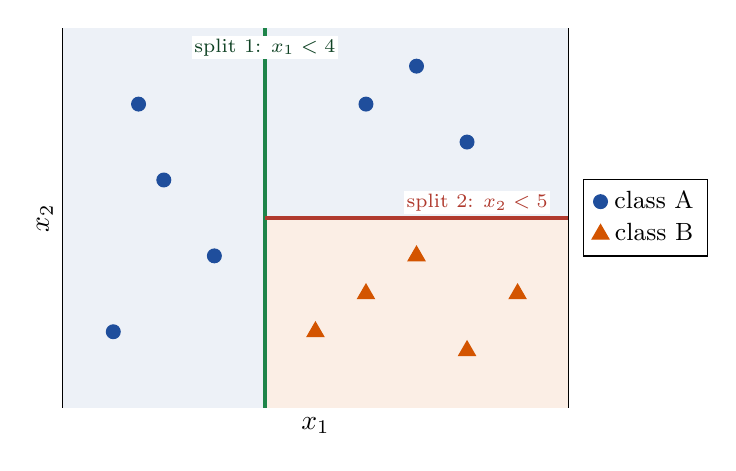
\begin{tikzpicture}
\begin{axis}[width=8cm,height=6.4cm,xmin=0,xmax=10,ymin=0,ymax=10,xlabel={$x_1$},ylabel={$x_2$},ticks=none,
  legend style={at={(1.03,0.5)},anchor=west,font=\small}]
\fill[mlblue!8] (axis cs:0,0) rectangle (axis cs:4,10);
\fill[mlorange!10] (axis cs:4,0) rectangle (axis cs:10,5);
\fill[mlblue!8] (axis cs:4,5) rectangle (axis cs:10,10);
\addplot[only marks,mark=*,mlblue,mark size=2.5pt] coordinates {(1,2)(2,6)(3,4)(1.5,8)(6,8)(8,7)(7,9)};
\addlegendentry{class A}
\addplot[only marks,mark=triangle*,mlorange,mark size=3.5pt] coordinates {(5,2)(6,3)(8,1.5)(7,4)(9,3)};
\addlegendentry{class B}
\draw[very thick,mlgreen] (axis cs:4,0)--(axis cs:4,10);
\draw[very thick,mlred] (axis cs:4,5)--(axis cs:10,5);
\node[font=\scriptsize,mlgreen!50!black,fill=white,inner sep=1pt] at (axis cs:4,9.5) {split 1: $x_1<4$};
\node[font=\scriptsize,mlred,fill=white,inner sep=1pt] at (axis cs:8.2,5.4) {split 2: $x_2<5$};
\end{axis}
\end{tikzpicture}
\caption{A decision tree with two splits carves the feature space into axis-parallel rectangles.}\label{fig:partition}
\end{figure}

\begin{explain}
Every split in a tree tests \emph{one feature against a threshold}, which draws a \textbf{straight line parallel to an axis}. The \textbf{green vertical line} is the root test $x_1<4$: everything to its left is class~A. On the right, the \textbf{red horizontal line} tests $x_2<5$: below it is class~B (orange), above it class~A. The final result is three \emph{rectangular regions}, each assigned one class. Trees therefore produce \emph{boxy} decision boundaries, which suit data with axis-aligned structure but approximate diagonal boundaries only with many small steps.
\end{explain}


\subsection{Overfitting and Pruning}

A tree allowed to grow until every leaf is pure will memorise the training data, noise included (low bias, \textbf{high variance}; see Chapter~2). We control complexity by \textbf{pruning}.

\begin{center}
\begin{tabular}{@{}p{3.3cm}p{10.2cm}@{}}
\toprule
\textbf{Pre-pruning} (early stopping) & Stop growing early: limit the depth (\texttt{max\_depth}), require a minimum number of samples to split (\texttt{min\_samples\_split}) or in a leaf (\texttt{min\_samples\_leaf}), or require a minimum gain.\\
\textbf{Post-pruning} & Grow the full tree, then \emph{cut back} branches that do not improve accuracy on a validation set (reduced-error pruning) or minimise cost $=\text{error}+\alpha\cdot(\text{number of leaves})$ (cost-complexity pruning).\\
\bottomrule
\end{tabular}
\end{center}

\subsection{Strengths and Weaknesses}

\begin{center}
\begin{tabular}{@{}p{6.7cm}p{6.7cm}@{}}
\toprule
\textbf{Advantages} & \textbf{Disadvantages}\\
\midrule
Easy to understand and visualise; human-readable rules & Prone to overfitting\\
Handles numeric and categorical features & Unstable: small data changes can give a very different tree\\
No feature scaling needed & Axis-parallel (boxy) boundaries only\\
Fast prediction; performs feature selection implicitly & Biased towards features with many values\\
\bottomrule
\end{tabular}
\end{center}

The instability of single trees is fixed by combining many of them into \emph{ensembles} such as Random Forests (Chapter~5).

%====================================================================
\procon{Decision trees}
{\item Easy to understand, visualise and convert to rules
 \item Handles numeric and categorical features; no scaling needed
 \item Fast prediction}
{\item Prone to overfitting; needs pruning
 \item Unstable: small data changes can change the tree
 \item Only axis-parallel (boxy) boundaries}
{\item Credit approval and medical diagnosis
 \item Customer churn prediction
 \item Rule extraction; base learner in Random Forests}

\section{Naive Bayes}

\subsection{Bayes' Theorem}

\begin{definition}[: Bayes' theorem]
For a class $C$ and observed evidence $\vect{x}$,
\[
  P(C\mid\vect{x})=\frac{P(\vect{x}\mid C)\,P(C)}{P(\vect{x})},\qquad
  P(\vect{x})=\sum_{c}P(\vect{x}\mid c)P(c).
\]
Here $P(C\mid\vect{x})$ is the \textbf{posterior}, $P(\vect{x}\mid C)$ the \textbf{likelihood}, $P(C)$ the \textbf{prior} and $P(\vect{x})$ the \textbf{evidence}.
\end{definition}

It follows directly from the definition of conditional probability, $P(C\mid\vect{x})P(\vect{x})=P(\vect{x},C)=P(\vect{x}\mid C)P(C)$. In words: \emph{posterior} (what we believe after seeing the evidence) $\propto$ \emph{likelihood} (how well the class explains the evidence) $\times$ \emph{prior} (what we believed before).

\begin{example}[: Spam and the word ``offer'']
Suppose 30\% of all e-mail is spam, so $P(\text{spam})=0.3$ and $P(\text{ham})=0.7$. The word ``offer'' occurs in 60\% of spam, $P(\text{offer}\mid\text{spam})=0.6$, but only in 10\% of ham, $P(\text{offer}\mid\text{ham})=0.1$. An e-mail contains ``offer''. How likely is it to be spam?
\[
P(\text{spam}\mid\text{offer})=\frac{0.6\times0.3}{0.6\times0.3+0.1\times0.7}=\frac{0.18}{0.18+0.07}=\frac{0.18}{0.25}=\mathbf{0.72}.
\]
\end{example}

\begin{figure}[!htbp]
\centering
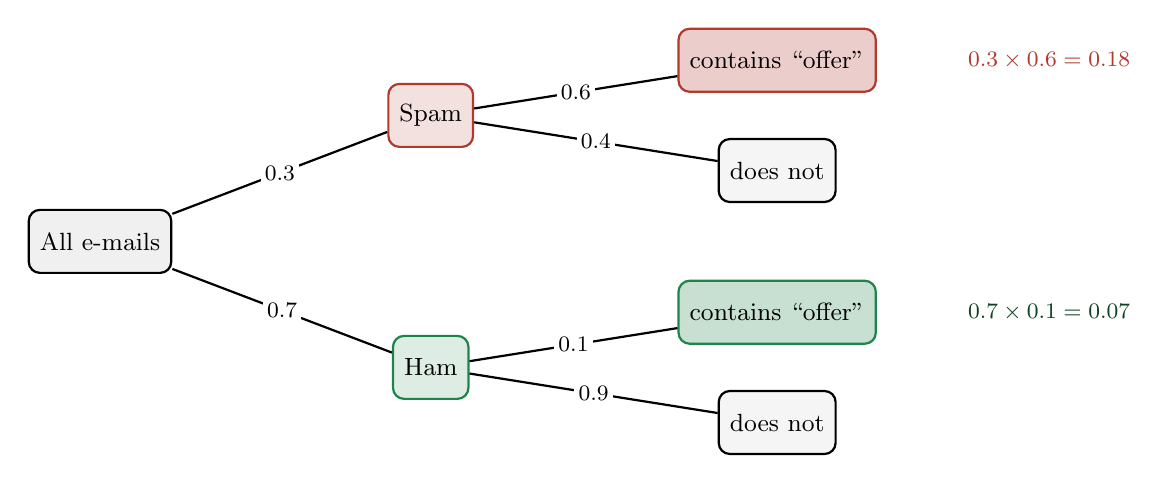
\begin{tikzpicture}[
  every node/.style={font=\small},
  lvl/.style={draw,rounded corners,thick,minimum height=0.8cm,inner sep=4pt},
  lab/.style={fill=white,inner sep=1.5pt,font=\footnotesize}]
\node[lvl,fill=gray!12] (r) at (0,0) {All e-mails};
\node[lvl,fill=mlred!15,draw=mlred] (s) at (4.2,1.6) {Spam};
\node[lvl,fill=mlgreen!15,draw=mlgreen] (h) at (4.2,-1.6) {Ham};
\node[lvl,fill=mlred!25,draw=mlred] (so) at (8.6,2.3) {contains ``offer''};
\node[lvl,fill=gray!8] (sn) at (8.6,0.9) {does not};
\node[lvl,fill=mlgreen!25,draw=mlgreen] (ho) at (8.6,-0.9) {contains ``offer''};
\node[lvl,fill=gray!8] (hn) at (8.6,-2.3) {does not};
\draw[thick] (r)--(s) node[midway,lab]{$0.3$};
\draw[thick] (r)--(h) node[midway,lab]{$0.7$};
\draw[thick] (s)--(so) node[midway,lab]{$0.6$};
\draw[thick] (s)--(sn) node[midway,lab]{$0.4$};
\draw[thick] (h)--(ho) node[midway,lab]{$0.1$};
\draw[thick] (h)--(hn) node[midway,lab]{$0.9$};
\node[font=\footnotesize,anchor=west,mlred] at (10.9,2.3) {$0.3\times0.6=0.18$};
\node[font=\footnotesize,anchor=west,mlgreen!50!black] at (10.9,-0.9) {$0.7\times0.1=0.07$};
\end{tikzpicture}
\caption{Probability tree for the spam example. Only the two ``offer'' leaves matter once we know the word appeared.}\label{fig:bayestree}
\end{figure}

\begin{explain}
Read the tree \textbf{left to right}, \emph{multiplying probabilities along a path}. First the e-mail is spam (0.3) or ham (0.7). Then, given its class, it contains ``offer'' with probability 0.6 (spam) or 0.1 (ham). The \textbf{two paths that end in ``contains offer''} have joint probabilities $0.18$ (spam) and $0.07$ (ham). Because we \emph{know} the word appeared, we only look at those two paths, and the posterior is the spam share of their total: $0.18/(0.18+0.07)=0.72$. The prior of 30\% has been \textbf{updated} to 72\% by the evidence.
\end{explain}

\subsection{The Naive Bayes Classifier}


\begin{definition}[: Naive Bayes classifier]
\textbf{Naive Bayes} is a \emph{supervised, probabilistic} classifier based on \textbf{Bayes' theorem} with the ``naive'' assumption that features are \emph{conditionally independent} given the class: $\hat y=\argmax_c P(c)\prod_jP(x_j\mid c)$.
\end{definition}


With many features $\vect{x}=(x_1,\dots,x_d)$, the likelihood $P(x_1,\dots,x_d\mid C)$ would need an enormous number of probabilities. Naive Bayes makes one simplifying assumption.

\begin{definition}[: Naive (conditional independence) assumption]
Given the class, the features are \textbf{independent}:
\[
  P(x_1,\dots,x_d\mid C)=\prod_{j=1}^{d}P(x_j\mid C).
\]
\end{definition}

The classification rule becomes (the denominator $P(\vect{x})$ is the same for every class, so it can be dropped):
\begin{equation}\label{eq:nb}
  \hat y=\argmax_{c}\; P(c)\prod_{j=1}^{d}P(x_j\mid c).
\end{equation}
The assumption is usually \emph{false} (in e-mail, ``free'' and ``offer'' tend to appear together), hence ``naive'', yet the classifier works surprisingly well, because we only need the class with the \emph{largest} score, not exact probabilities.

\paragraph{Training = counting.} Estimate $P(c)=N_c/N$ and $P(x_j=v\mid c)=\dfrac{\text{count}(x_j=v,\ \text{class }c)}{N_c}$ from the training data.

\subsection{Worked Example: Play-Tennis Again}

Classify the new day $\vect{x}=(\text{Sunny},\ \text{Cool},\ \text{High},\ \text{Strong})$ using the 14-day table.

\textbf{Priors:} $P(\text{Yes})=\tfrac9{14}$, $P(\text{No})=\tfrac5{14}$.

\begin{center}
\begin{tabular}{@{}lcc@{}}
\toprule
\textbf{Likelihood} & \textbf{Given Yes (9 days)} & \textbf{Given No (5 days)}\\
\midrule
$P(\text{Sunny}\mid\cdot)$ & $2/9$ & $3/5$\\
$P(\text{Cool}\mid\cdot)$ & $3/9$ & $1/5$\\
$P(\text{High}\mid\cdot)$ & $3/9$ & $4/5$\\
$P(\text{Strong}\mid\cdot)$ & $3/9$ & $3/5$\\
\bottomrule
\end{tabular}
\end{center}

\[
\text{score(Yes)}=\tfrac{9}{14}\cdot\tfrac29\cdot\tfrac39\cdot\tfrac39\cdot\tfrac39=0.00529,\qquad
\text{score(No)}=\tfrac{5}{14}\cdot\tfrac35\cdot\tfrac15\cdot\tfrac45\cdot\tfrac35=0.02057 .
\]
\textbf{Decision:} $0.02057>0.00529\Rightarrow$ predict \textbf{No}.\\
\textbf{Posterior probabilities} (normalise): $P(\text{No}\mid\vect{x})=\dfrac{0.02057}{0.02057+0.00529}=0.795$ and $P(\text{Yes}\mid\vect{x})=0.205$.


\subsection{Laplace Smoothing}

\begin{warning}
\textbf{The zero-frequency problem.} If a value never occurs with a class in training (e.g.\ ``Overcast'' never occurs with ``No''), then $P(\text{Overcast}\mid\text{No})=0$ and the \emph{whole product becomes zero}, whatever the other features say.
\end{warning}

\textbf{Laplace (add-one) smoothing} adds a pseudo-count $\alpha$ (usually $1$) to every count:
\[
  P(x_j=v\mid c)=\frac{\text{count}(x_j=v,c)+\alpha}{N_c+\alpha V_j},
\]
where $V_j$ is the number of different values of feature $j$.

\begin{example}[: Smoothing]
$\text{count}(\text{Overcast},\text{No})=0$, $N_{\text{No}}=5$, and Outlook has $V=3$ values. With $\alpha=1$: $P(\text{Overcast}\mid\text{No})=\dfrac{0+1}{5+3}=\dfrac18=0.125$ instead of $0$.
\end{example}

\subsection{Variants of Naive Bayes}

\begin{center}
\begin{tabular}{@{}p{3.4cm}p{4.6cm}p{5.2cm}@{}}
\toprule
\textbf{Variant} & \textbf{Feature type} & \textbf{Model for $P(x_j\mid c)$}\\
\midrule
Gaussian & Continuous & Normal density with class-wise mean $\mu_{jc}$ and variance $\sigma_{jc}^2$\\
Multinomial & Counts (word counts) & Relative frequency of word in class (with smoothing)\\
Bernoulli & Binary (word present/absent) & Probability of presence/absence\\
\bottomrule
\end{tabular}
\end{center}

For the \textbf{Gaussian} variant,
\[
  P(x_j\mid c)=\frac{1}{\sqrt{2\pi}\,\sigma_{jc}}\exp\!\left(-\frac{(x_j-\mu_{jc})^2}{2\sigma_{jc}^2}\right).
\]

\begin{example}[: Gaussian Naive Bayes with one feature]
Heights: males have $\mu=175$, $\sigma=7$ cm; females have $\mu=162$, $\sigma=6$ cm; priors are equal. Classify a person of height $170$ cm.
\begin{align*}
P(170\mid\text{male})&=\tfrac{1}{7\sqrt{2\pi}}e^{-25/98}=0.0570\times0.775=0.0442,\\
P(170\mid\text{female})&=\tfrac{1}{6\sqrt{2\pi}}e^{-64/72}=0.0665\times0.411=0.0273.
\end{align*}
Since the priors are equal, the larger likelihood wins: \textbf{male}, with posterior $0.0442/(0.0442+0.0273)\approx0.62$. (Only 62\% confident because $170$ is plausible for both.)
\end{example}

\begin{keyidea}
\textbf{Numerical tip.} Multiplying many small probabilities underflows to $0$. Real implementations add \textbf{logarithms} instead: $\hat y=\argmax_c\big[\ln P(c)+\sum_j\ln P(x_j\mid c)\big]$.
\end{keyidea}

\begin{center}
\begin{tabular}{@{}p{6.7cm}p{6.7cm}@{}}
\toprule
\textbf{Advantages} & \textbf{Disadvantages}\\
\midrule
Very fast to train and predict (just counting) & Independence assumption rarely true\\
Works well with little data and many features & Probability estimates can be poorly calibrated\\
Excellent baseline for text (spam, sentiment) & Zero-frequency problem (needs smoothing)\\
Handles multiple classes naturally & Cannot learn interactions between features\\
\bottomrule
\end{tabular}
\end{center}

%====================================================================
\procon{Naive Bayes}
{\item Very fast to train and predict
 \item Works well with little data and many features
 \item Excellent baseline for text classification}
{\item Independence assumption is rarely true
 \item Probability estimates can be poorly calibrated
 \item Zero-frequency problem (needs smoothing)}
{\item Spam filtering
 \item Sentiment analysis
 \item Document and news classification
 \item Medical diagnosis}

\section{Putting It Together: The Three Methods in Python}

\begin{tryit}
Compare all three on the classic \emph{Iris} flower dataset (150 flowers, 4 measurements, 3 species).
\begin{lstlisting}
from sklearn.datasets import load_iris
from sklearn.model_selection import train_test_split, cross_val_score
from sklearn.preprocessing import StandardScaler
from sklearn.pipeline import make_pipeline
from sklearn.neighbors import KNeighborsClassifier
from sklearn.tree import DecisionTreeClassifier
from sklearn.naive_bayes import GaussianNB

X, y = load_iris(return_X_y=True)
Xtr, Xte, ytr, yte = train_test_split(
    X, y, test_size=0.3, random_state=42, stratify=y)

models = {
  "k-NN (k=5)": make_pipeline(StandardScaler(),
                              KNeighborsClassifier(n_neighbors=5)),
  "Decision tree": DecisionTreeClassifier(max_depth=3, random_state=0),
  "Naive Bayes": GaussianNB(),
}
for name, m in models.items():
    m.fit(Xtr, ytr)
    cv = cross_val_score(m, X, y, cv=5).mean()
    print(f"{name:14s} test = {m.score(Xte, yte):.3f}  CV = {cv:.3f}")
\end{lstlisting}
\textbf{Output:}
\begin{center}
\begin{tabular}{@{}lcc@{}}
\toprule
\textbf{Model} & \textbf{Test accuracy} & \textbf{5-fold CV accuracy}\\
\midrule
k-NN ($k=5$) & 0.911 & 0.960\\
Decision tree (depth 3) & 0.933 & 0.960\\
Naive Bayes & 0.911 & 0.953\\
\bottomrule
\end{tabular}
\end{center}
All three do well here. The single test split (45 flowers) is noisy, so the \emph{cross-validated} numbers are more reliable and show the methods are practically tied.

\medskip\noindent\textbf{Effect of $k$} (same data, scaled):
\begin{center}
\begin{tabular}{@{}cccl@{}}
\toprule
$k$ & Train acc. & Test acc. & Comment\\
\midrule
1 & 1.000 & 0.933 & memorises training data\\
3 & 0.971 & 0.911 & \\
5 & 0.981 & 0.911 & \\
15 & 0.981 & 0.933 & smooth boundary\\
51 & 0.876 & 0.822 & \textbf{underfits}: both fall\\
\bottomrule
\end{tabular}
\end{center}
A huge $k$ averages over too much of the data and accuracy drops on \emph{both} sets: underfitting, exactly as predicted.

\medskip\noindent\textbf{A tiny tree you can read} (\texttt{max\_depth=2}, printed with \texttt{export\_text}):
\begin{lstlisting}[numbers=none]
|--- petal_wid <= 0.70            -> class 0 (setosa)
|--- petal_wid >  0.70
|   |--- petal_wid <= 1.55       -> class 1 (versicolor)
|   |--- petal_wid >  1.55       -> class 2 (virginica)
\end{lstlisting}
Just \emph{two questions about petal width} separate the three species.
\end{tryit}

\section{Comparison of the Three Methods}

\begin{center}
\small
\begin{tabular}{@{}p{3.1cm}p{3.5cm}p{3.5cm}p{3.5cm}@{}}
\toprule
 & \textbf{k-NN} & \textbf{Decision tree} & \textbf{Naive Bayes}\\
\midrule
Learner type & Lazy, instance-based & Eager, model-based & Eager, model-based\\
Training cost & None & Moderate & Very low\\
Prediction cost & High & Very low & Very low\\
Assumption & Similar points share classes & Axis-aligned splits & Features independent given class\\
Needs scaling? & \textbf{Yes} & No & No (Gaussian: no)\\
Interpretable? & Low & \textbf{High} & Moderate\\
Main hyperparameter & $k$, metric & depth, min samples & smoothing $\alpha$\\
Typical weakness & Slow; high dimensions & Overfits; unstable & Independence assumption\\
\bottomrule
\end{tabular}
\end{center}

%====================================================================
\begin{summary}
\begin{itemize}
  \item Distance measures ($L_1,L_2,L_p,L_\infty$, Hamming, cosine) define similarity; \textbf{scale features} first (min--max or z-score, fitted on training data only).
  \item \textbf{k-NN} stores data and predicts by majority vote (classification) or mean (regression) of the $k$ closest points. Small $k$ $\Rightarrow$ high variance; large $k$ $\Rightarrow$ high bias.
  \item \textbf{Decision trees} split on the feature with highest \textbf{information gain} (entropy) or largest Gini reduction. Full trees overfit; control with \textbf{pruning}.
  \item Entropy $H=-\sum p_i\log_2p_i$; Gini $=1-\sum p_i^2$; Gain $=H(S)-\sum\frac{|S_v|}{|S|}H(S_v)$.
  \item \textbf{Naive Bayes}: $\hat y=\argmax_c P(c)\prod_jP(x_j\mid c)$, assuming conditional independence; use \textbf{Laplace smoothing} and log-probabilities; variants: Gaussian, multinomial, Bernoulli.
  \item In the Play-Tennis example the tree root is Outlook (gain $0.247$) and Naive Bayes predicts ``No'' with posterior $0.795$ for (Sunny, Cool, High, Strong).
\end{itemize}
\end{summary}

%====================================================================
\section*{Exam Corner}
\addcontentsline{toc}{section}{Exam Corner}

\subsection*{A.\ Very Short Answer Questions (2 marks each)}
\begin{enumerate}
  \item Define Euclidean and Manhattan distance. \qmarks{2}
  \item Why is feature scaling necessary for k-NN? \qmarks{2}
  \item Why is k-NN called a lazy learner? \qmarks{2}
  \item What happens when $k=1$ and when $k=n$ in k-NN? \qmarks{2}
  \item Define entropy and Gini index. \qmarks{2}
  \item What is information gain? \qmarks{2}
  \item What is pruning? Name its two types. \qmarks{2}
  \item State Bayes' theorem. \qmarks{2}
  \item Why is Naive Bayes called ``naive''? \qmarks{2}
  \item What is Laplace smoothing and why is it needed? \qmarks{2}
\end{enumerate}

\begin{modelans}[: Q4 and Q10]
\textbf{Q4.} For $k=1$ the prediction is the label of the single nearest point: the boundary is very jagged, bias is low, variance is high (overfitting). For $k=n$ every query gets the overall majority class: the model is a constant, bias is high and variance is zero (underfitting).\par
\textbf{Q10.} Laplace smoothing adds a pseudo-count (usually 1) to every feature-value count so that $P(x_j\mid c)=\frac{\text{count}+1}{N_c+V_j}$. It is needed to avoid zero probabilities for unseen feature--class combinations, which would force the whole product $\prod P(x_j\mid c)$ to zero.
\end{modelans}

\subsection*{B.\ Short Answer Questions (5 marks each)}
\begin{enumerate}
  \item Explain the k-NN algorithm for classification with an example. \qmarks{5}
  \item Discuss the effect of the value of $k$ on k-NN (bias, variance, over/underfitting). \qmarks{5}
  \item List the advantages and disadvantages of k-NN. What is the curse of dimensionality? \qmarks{5}
  \item Explain the structure of a decision tree. Differentiate entropy and Gini index. \qmarks{5}
  \item Explain overfitting in decision trees. How can it be reduced? \qmarks{5}
  \item Explain the Naive Bayes classifier and its independence assumption. \qmarks{5}
  \item Compare k-NN, decision trees and Naive Bayes in a table. \qmarks{5}
\end{enumerate}

\begin{modelans}[: B4 (outline for 5 marks)]
\emph{Structure:} root node (first test), internal nodes (feature tests), branches (outcomes), leaves (class label or value); classification of a new point follows the path from root to a leaf.\par
\emph{Entropy} $H=-\sum p_i\log_2p_i$: measures disorder of class labels; $0$ for a pure node, $1$ for a 50/50 binary node.
\emph{Gini} $=1-\sum p_i^2$: probability of mis-classifying a random item; $0$ for pure, $0.5$ for 50/50.\par
\begin{center}\small
\begin{tabular}{@{}lll@{}}
\toprule
 & \textbf{Entropy} & \textbf{Gini}\\
\midrule
Formula & $-\sum p_i\log_2 p_i$ & $1-\sum p_i^2$\\
Range (2 classes) & $0$ to $1$ & $0$ to $0.5$\\
Cost & Needs logarithm & Cheaper (no log)\\
Used in & ID3, C4.5 & CART\\
\bottomrule
\end{tabular}
\end{center}
\end{modelans}

\subsection*{C.\ Long Answer Questions (10 marks each)}
\begin{enumerate}
  \item Explain the ID3 algorithm. Using the 14-day Play-Tennis table, compute the information gain of \emph{Outlook} and show that it is chosen as the root. \qmarks{10}
  \item Explain the Naive Bayes classifier with Laplace smoothing. Use the Play-Tennis data to classify (Sunny, Cool, High, Strong). \qmarks{10}
  \item Describe the k-NN algorithm for classification and regression. Illustrate with a numerical example and discuss the choice of $k$ and distance metric. \qmarks{10}
  \item Explain distance measures used in machine learning with examples. Why must features be scaled? \qmarks{10}
  \item Discuss pre-pruning and post-pruning in decision trees. How do trees compare to k-NN and Naive Bayes in terms of interpretability and cost? \qmarks{10}
\end{enumerate}

\begin{modelans}[: C1 (key steps)]
1.~$H(S)=0.940$ (9 Yes, 5 No).\quad
2.~Outlook: Sunny (2Y,3N) $H=0.971$; Overcast (4Y,0N) $H=0$; Rain (3Y,2N) $H=0.971$.\quad
3.~$\text{Gain}=0.940-\tfrac5{14}(0.971)-\tfrac4{14}(0)-\tfrac5{14}(0.971)=0.247$.\quad
4.~Gains of the others: Humidity $0.152$, Wind $0.048$, Temperature $0.029$. Outlook is largest, so it is the root.\quad
5.~Overcast is pure (Yes); Sunny splits on Humidity; Rain splits on Wind. Draw the tree of Figure~\ref{fig:tree}.
\end{modelans}

\subsection*{D.\ Numerical Problems}
\begin{enumerate}
  \item Find the Euclidean and Manhattan distance between $(2,3)$ and $(6,6)$. \textit{(Answer: $5$ and $7$.)}
  \item Training points: $(1,2)$ A, $(2,1)$ A, $(3,3)$ A, $(4,5)$ B, $(5,4)$ B. Classify the query $(4,4)$ using $k=3$ and $k=5$ (Euclidean). \textit{(Distances: $1,1,1.414,3.606,3.606$. Answer: $k=3$: B,B,A $\to$ \textbf{B}; $k=5$: 2B vs 3A $\to$ \textbf{A}.)}
  \item Distances to a query are $1$ and $2$ with target values $10$ and $20$. Give the weighted ($1/d$) k-NN regression value for $k=2$. \textit{(Answer: $\frac{1\cdot10+0.5\cdot20}{1.5}=13.33$.)}
  \item Compute the entropy of a node with 6 positive and 2 negative examples. \textit{(Answer: $-0.75\log_2 0.75-0.25\log_2 0.25=0.811$.)}
  \item A node with 4 positives and 4 negatives is split into $(3+,1-)$ and $(1+,3-)$. Compute the information gain. \textit{(Answer: $1-\tfrac48(0.811)-\tfrac48(0.811)=0.189$.)}
  \item Compute the Gini index of a node with 3 ``yes'' and 1 ``no''. \textit{(Answer: $1-0.5625-0.0625=0.375$.)}
  \item $P(\text{spam})=0.4$, $P(\text{``free''}\mid\text{spam})=0.5$, $P(\text{``free''}\mid\text{ham})=0.05$. Find $P(\text{spam}\mid\text{``free''})$. \textit{(Answer: $\frac{0.4\cdot0.5}{0.4\cdot0.5+0.6\cdot0.05}=\frac{0.20}{0.23}=0.870$.)}
  \item A word never appears in the 100 words of class ``ham''; vocabulary size is 50. Find its smoothed probability. \textit{(Answer: $\frac{0+1}{100+50}=0.0067$.)}
\end{enumerate}

\subsection*{E.\ Multiple-Choice Questions}
\begin{enumerate}
  \item k-NN does its main computation during: \\
  (a) training \quad (b) prediction \quad (c) pruning \quad (d) scaling
  \item Which distance is the sum of absolute coordinate differences? \\
  (a) Euclidean \quad (b) Chebyshev \quad (c) Manhattan \quad (d) Cosine
  \item The entropy of a pure node is: \\
  (a) 1 \quad (b) 0.5 \quad (c) 0 \quad (d) $\infty$
  \item A decision tree chooses the split with the: \\
  (a) lowest gain \quad (b) highest information gain \quad (c) most branches \quad (d) fewest samples
  \item Which method needs feature scaling the most? \\
  (a) Decision tree \quad (b) Naive Bayes \quad (c) k-NN \quad (d) none
  \item Overfitting of a decision tree is reduced by: \\
  (a) growing it deeper \quad (b) pruning \quad (c) removing the root \quad (d) adding duplicate data
  \item In Naive Bayes the features are assumed to be: \\
  (a) identical \quad (b) correlated \quad (c) conditionally independent given the class \quad (d) Gaussian only
  \item Laplace smoothing prevents: \\
  (a) overfitting of trees \quad (b) zero probabilities \quad (c) scaling errors \quad (d) ties in k-NN
  \item The Gini index of a 50/50 two-class node is: \\
  (a) 1 \quad (b) 0.5 \quad (c) 0.25 \quad (d) 0
  \item A very large $k$ in k-NN typically causes: \\
  (a) overfitting \quad (b) underfitting \quad (c) zero error \quad (d) no change
\end{enumerate}
\textbf{Answers:} 1-b,\ 2-c,\ 3-c,\ 4-b,\ 5-c,\ 6-b,\ 7-c,\ 8-b,\ 9-b,\ 10-b.

\subsection*{F.\ Practice Problems}
\begin{enumerate}
  \item Using the Play-Tennis table, find the best feature to split on inside the \emph{Sunny} branch using information gain, and verify that Humidity gives gain $0.971$.
  \item Classify (Overcast, Mild, High, Weak) with Naive Bayes using add-one smoothing.
  \item \textbf{Coding:} using \texttt{sklearn}, plot training and test accuracy of k-NN on Iris for $k=1,3,\dots,31$ and identify the best $k$ by 5-fold cross-validation.
  \item \textbf{Coding:} fit \texttt{DecisionTreeClassifier} with \texttt{max\_depth} from 1 to 10 and plot train vs.\ test accuracy. At which depth does overfitting begin?
\end{enumerate}

\begin{revision}
\begin{center}\small
\begin{tabular}{@{}p{3.6cm}p{9.6cm}@{}}
\toprule
\textbf{Topic} & \textbf{One-line recall}\\
\midrule
Euclidean / Manhattan & $\sqrt{\sum(a_i-b_i)^2}$ / $\sum|a_i-b_i|$.\\
Scaling & Min--max $\frac{x-x_{\min}}{x_{\max}-x_{\min}}$; z-score $\frac{x-\mu}{\sigma}$; fit on train only.\\
k-NN & Lazy; majority vote / mean of $k$ closest; small $k$ overfits, large $k$ underfits.\\
Weighted k-NN & $w_i=1/d_i$; closer neighbours count more.\\
Entropy / Gini & $-\sum p\log_2p$ / $1-\sum p^2$; both $0$ if pure.\\
Information gain & $H(S)-\sum\frac{|S_v|}{|S|}H(S_v)$; choose the maximum.\\
Pruning & Pre (max depth, min samples) / post (cut back, cost-complexity).\\
Tree boundary & Axis-parallel rectangles.\\
Bayes' theorem & Posterior $=$ likelihood $\times$ prior $/$ evidence.\\
Naive Bayes & $\argmax_cP(c)\prod_jP(x_j\mid c)$; conditional independence; Laplace $\frac{n+1}{N_c+V}$.\\
Play-Tennis results & Root Outlook (gain $0.247$); NB for (S,C,H,Str): No, $P=0.795$.\\
\bottomrule
\end{tabular}
\end{center}
\end{revision}

\chapter[Linear Models and Support Vector Machines]{Linear Models and\\Support Vector Machines}
\label{ch:linear}
\begin{objectives}
After studying this chapter you will be able to:
\begin{itemize}
  \item \textbf{define} linear regression, logistic regression, generalized linear models and support vector machines, and write each as a standard exam answer;
  \item fit a regression line by hand, using both the \textbf{least-squares formula} and \textbf{gradient descent}, and judge it with \textbf{MSE} and $R^2$;
  \item explain the \textbf{sigmoid}, \textbf{odds}, \textbf{log-odds} and \textbf{cross-entropy loss}, and compute logistic-regression probabilities, boundaries and accuracy end to end;
  \item describe the three components of a \textbf{GLM} and work with \textbf{Poisson regression};
  \item explain \textbf{binary classification}, the \textbf{maximum-margin hyperplane}, \textbf{support vectors} and the \textbf{soft margin}, and solve a small SVM by hand;
  \item compare linear and logistic regression and say when to use each;
  \item answer 2-, 5- and 10-mark university questions on Unit~II.
\end{itemize}
\end{objectives}

\begin{pullquote}[--- Leo Breiman]
Simple models are not simple-minded: a good linear model often beats a clever complicated one.
\end{pullquote}

In Chapter~3 the models were built from \emph{distances}, \emph{questions} and \emph{probabilities}. This chapter studies the most widely used family of models in all of statistics and machine learning: \textbf{linear models}, which predict from a \emph{weighted sum} of the features.

\begin{definition}[: Linear model]
A \textbf{linear model} computes a score
\[
  z=\vect{w}\cdot\vect{x}+b=w_1x_1+w_2x_2+\cdots+w_dx_d+b,
\]
where $\vect{w}$ are the \textbf{weights} (coefficients) and $b$ is the \textbf{bias} (intercept). The final prediction is a function of $z$: $z$ itself (linear regression), a probability $\sigma(z)$ (logistic regression), or the sign of $z$ (SVM).
\end{definition}

\begin{center}\small
\begin{tabular}{@{}llll@{}}
\toprule
\textbf{Model} & \textbf{Prediction from the score $z$} & \textbf{Output} & \textbf{Real-life task}\\
\midrule
Linear regression & $\hat y=z$ & any real number & Marks from study hours\\
Logistic regression & $\hat p=\dfrac1{1+e^{-z}}$ & probability in $(0,1)$ & Will the student pass?\\
GLM (Poisson) & $\hat\mu=e^{z}$ & non-negative count & Number of calls per day\\
SVM & $\hat y=\operatorname{sign}(z)$ & class $-1$ or $+1$ & Spam or not spam\\
\bottomrule
\end{tabular}
\end{center}

%====================================================================
\section{Linear Regression}


\begin{definition}[: Linear regression]
\textbf{Linear regression} is a \emph{supervised, parametric} learning method for \emph{regression} problems. It models the target $y$ as a \textbf{linear function of the input features} plus random error, $y=\theta_0+\theta_1x_1+\cdots+\theta_dx_d+\varepsilon$, and chooses the parameters that minimise the sum of squared prediction errors (\textbf{method of least squares}).
\end{definition}



\paragraph{Assumptions of linear regression}
\begin{itemize}
  \item Linearity of the relationship
  \item Independence of errors
  \item Constant error variance (homoscedasticity)
  \item Normally distributed errors (for inference)
  \item No strong multicollinearity among features
\end{itemize}

\subsection{Simple Linear Regression}

With one feature $x$ the model is a straight line
\[
  \hat y=\theta_0+\theta_1x,
\]
where $\theta_1$ is the \textbf{slope} (change in $y$ per unit change in $x$) and $\theta_0$ the \textbf{intercept} (value of $y$ at $x=0$). The error of a prediction is the \textbf{residual} $e_i=y_i-\hat y_i$. The method of \textbf{least squares} chooses $\theta_0,\theta_1$ to minimise the \textbf{sum of squared errors}
\[
  \text{SSE}=\sum_{i=1}^{n}(y_i-\theta_0-\theta_1x_i)^2 .
\]
Setting the partial derivatives $\partial\text{SSE}/\partial\theta_0$ and $\partial\text{SSE}/\partial\theta_1$ to zero gives the \textbf{closed-form solution}
\begin{equation}\label{eq:ols}
  \theta_1=\frac{\sum_i(x_i-\bar x)(y_i-\bar y)}{\sum_i(x_i-\bar x)^2}=\frac{S_{xy}}{S_{xx}},\qquad
  \theta_0=\bar y-\theta_1\bar x .
\end{equation}

\subsubsection*{Real-life example: study hours and exam marks}

A teacher records the hours studied $x$ and the marks $y$ (out of 100) of five students.

\begin{center}
\begin{tabular}{@{}c|ccccc|c@{}}
\toprule
Student & A & B & C & D & E & Mean\\
\midrule
Hours $x$ & 1 & 2 & 3 & 4 & 5 & $\bar x=3$\\
Marks $y$ & 35 & 45 & 50 & 65 & 70 & $\bar y=53$\\
\bottomrule
\end{tabular}
\end{center}

\begin{example}[: End-to-end solution]
\textbf{Step 1: deviations from the mean.}
\begin{center}
\begin{tabular}{@{}c|ccccc|c@{}}
\toprule
$x-\bar x$ & $-2$ & $-1$ & $0$ & $1$ & $2$ & \\
$y-\bar y$ & $-18$ & $-8$ & $-3$ & $12$ & $17$ & \\
$(x-\bar x)(y-\bar y)$ & $36$ & $8$ & $0$ & $12$ & $34$ & $S_{xy}=90$\\
$(x-\bar x)^2$ & $4$ & $1$ & $0$ & $1$ & $4$ & $S_{xx}=10$\\
\bottomrule
\end{tabular}
\end{center}
\textbf{Step 2: parameters.} $\theta_1=\dfrac{90}{10}=9$ and $\theta_0=53-9(3)=26$. \textbf{Model:} $\ \widehat{\text{marks}}=26+9\times\text{hours}$.\par
\textbf{Interpretation:} each extra hour of study adds about \textbf{9 marks}; a student who studies 0 hours is expected to score 26.\par
\textbf{Step 3: predict.} For $x=6$ hours: $\hat y=26+9(6)=\mathbf{80}$ marks.\par
\textbf{Step 4: check the fit.}
\begin{center}
\begin{tabular}{@{}c|ccccc|c@{}}
\toprule
$x$ & 1 & 2 & 3 & 4 & 5 & \\
$y$ & 35 & 45 & 50 & 65 & 70 & \\
$\hat y=26+9x$ & 35 & 44 & 53 & 62 & 71 & \\
Residual $y-\hat y$ & 0 & 1 & $-3$ & 3 & $-1$ & $\sum e=0$\\
$e^2$ & 0 & 1 & 9 & 9 & 1 & $\text{SSE}=20$\\
$(y-\bar y)^2$ & 324 & 64 & 9 & 144 & 289 & $\text{SST}=830$\\
\bottomrule
\end{tabular}
\end{center}
\[
  \text{MSE}=\frac{\text{SSE}}{n}=\frac{20}{5}=4,\quad
  \text{RMSE}=2,\quad
  R^2=1-\frac{\text{SSE}}{\text{SST}}=1-\frac{20}{830}=\mathbf{0.976}.
\]
The line explains about \textbf{97.6\%} of the variation in marks. The residuals add up to $0$, a property of least squares with an intercept.
\end{example}

\begin{figure}[!htbp]
\centering
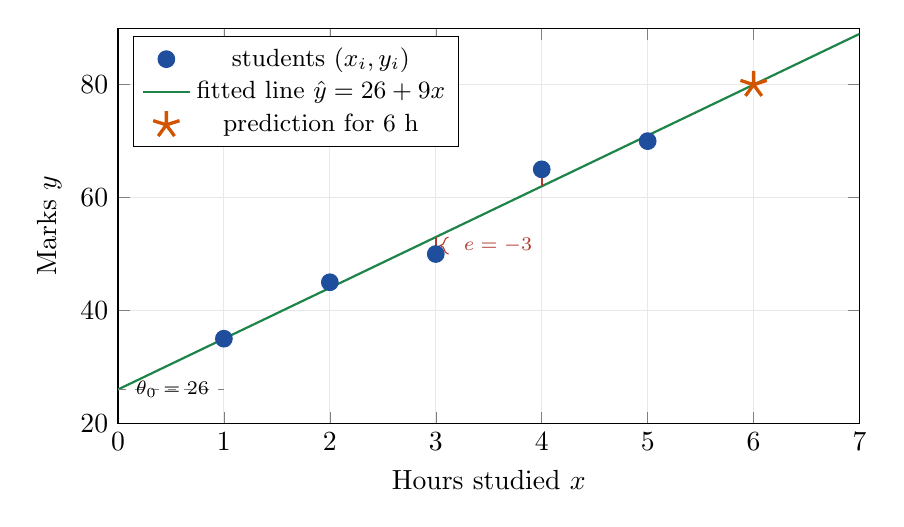
\begin{tikzpicture}
\begin{axis}[width=11cm,height=6.6cm,xlabel={Hours studied $x$},ylabel={Marks $y$},
  xmin=0,xmax=7,ymin=20,ymax=90,grid=both,grid style={gray!18},
  legend style={at={(0.02,0.98)},anchor=north west,font=\small}]
\addplot[only marks,mark=*,mlblue,mark size=3pt] coordinates {(1,35)(2,45)(3,50)(4,65)(5,70)};
\addlegendentry{students $(x_i,y_i)$}
\addplot[thick,mlgreen,domain=0:7]{26+9*x};
\addlegendentry{fitted line $\hat y=26+9x$}
\addplot[only marks,mark=star,mlorange,mark size=5pt,very thick] coordinates {(6,80)};
\addlegendentry{prediction for 6 h}
\draw[mlred,thick] (axis cs:2,44)--(axis cs:2,45);
\draw[mlred,thick] (axis cs:3,53)--(axis cs:3,50);
\draw[mlred,thick] (axis cs:4,62)--(axis cs:4,65);
\draw[mlred,thick] (axis cs:5,71)--(axis cs:5,70);
\draw[dashed,gray] (axis cs:0,26)--(axis cs:1,26);
\node[font=\scriptsize,anchor=east] at (axis cs:0.95,26) {$\theta_0=26$};
\draw[decorate,decoration={brace,amplitude=3pt},mlred] (axis cs:3.12,50)--(axis cs:3.12,53) node[midway,right,font=\scriptsize,xshift=2pt] {$e=-3$};
\end{axis}
\end{tikzpicture}
\caption{Least-squares line for study hours vs.\ marks. Red segments are residuals.}\label{fig:linreg}
\end{figure}

\begin{explain}
Each \textbf{blue dot} is a student. The \textbf{green line} is the best straight line, chosen so that the \emph{sum of the squared lengths of the red vertical segments} is as small as possible. A red segment is a \textbf{residual}: the gap between the actual marks and the line's prediction. For student C the line predicts 53 but the actual mark is 50, so the residual is $-3$. The \textbf{slope} of the line is 9 (marks per hour), and where it meets the vertical axis it gives the intercept 26. The \textbf{orange star} is the prediction for a student who studies 6 hours: we read the height of the line at $x=6$, giving 80.
\end{explain}

\subsection{Normal Equation (Matrix Form)}

For one or many features, stack the inputs into a matrix $\mathbf X$ with a leading column of ones (for the intercept) and the targets into a vector $\vect y$. Minimising $J$ gives the \textbf{normal equation}
\begin{equation}\label{eq:normal}
  \vect\theta=(\mathbf X^{\!\top}\mathbf X)^{-1}\mathbf X^{\!\top}\vect y .
\end{equation}

\begin{example}[: Same problem in matrix form]
With $\mathbf X=\begin{bmatrix}1&1\\1&2\\1&3\\1&4\\1&5\end{bmatrix}$ and $\vect y=(35,45,50,65,70)^{\top}$:
\[
\mathbf X^{\!\top}\mathbf X=\begin{bmatrix}5&15\\15&55\end{bmatrix},\quad
\mathbf X^{\!\top}\vect y=\begin{bmatrix}265\\885\end{bmatrix},\quad
(\mathbf X^{\!\top}\mathbf X)^{-1}=\frac1{50}\begin{bmatrix}55&-15\\-15&5\end{bmatrix}.
\]
\[
\vect\theta=\frac1{50}\begin{bmatrix}55(265)-15(885)\\-15(265)+5(885)\end{bmatrix}
=\frac1{50}\begin{bmatrix}1300\\450\end{bmatrix}=\begin{bmatrix}26\\9\end{bmatrix}.
\]
This is the same answer, $\theta_0=26$, $\theta_1=9$.
\end{example}

The normal equation is exact but requires inverting a $d\times d$ matrix (cost $\approx O(d^3)$), which is slow for thousands of features. For large problems we use an iterative method.

\subsection{Gradient Descent}

\begin{definition}[: Gradient descent]
\textbf{Gradient descent} is an iterative optimisation algorithm that minimises a differentiable loss $J(\vect\theta)$ by repeatedly moving the parameters a small step in the direction of \emph{steepest decrease}, i.e.\ opposite to the gradient:
\[
  \theta_j\;\leftarrow\;\theta_j-\alpha\,\frac{\partial J}{\partial\theta_j},\qquad j=0,1,\dots,d,
\]
where $\alpha>0$ is the \textbf{learning rate}. All parameters are updated \emph{simultaneously}.
\end{definition}

For linear regression with $J(\vect\theta)=\frac1{2n}\sum_i(\hat y_i-y_i)^2$:
\[
\frac{\partial J}{\partial\theta_0}=\frac1n\sum_i(\hat y_i-y_i),\qquad
\frac{\partial J}{\partial\theta_1}=\frac1n\sum_i(\hat y_i-y_i)\,x_i .
\]

\begin{example}[: Gradient descent by hand on the marks data]
Start at $\theta_0=\theta_1=0$ and use $\alpha=0.01$.\par
\textbf{Iteration 1.} Predictions are all $0$, so the errors $\hat y-y$ are $-35,-45,-50,-65,-70$.
\[
\tfrac{\partial J}{\partial\theta_0}=\tfrac{-265}{5}=-53,\qquad
\tfrac{\partial J}{\partial\theta_1}=\tfrac{-35-90-150-260-350}{5}=\tfrac{-885}{5}=-177 .
\]
\[
\theta_0=0-0.01(-53)=0.53,\qquad\theta_1=0-0.01(-177)=1.77 .
\]
\textbf{Iteration 2.} Predictions $0.53+1.77x$ are $2.30,\,4.07,\,5.84,\,7.61,\,9.38$; errors $-32.70,-40.93,-44.16,-57.39,-60.62$.
\[
\tfrac{\partial J}{\partial\theta_0}=-47.16,\quad\tfrac{\partial J}{\partial\theta_1}=-155.94\ \Rightarrow\ \theta_0=1.00,\ \theta_1=3.33 .
\]
\begin{center}
\begin{tabular}{@{}cccc@{}}
\toprule
\textbf{Iteration} & $\theta_0$ & $\theta_1$ & Loss $J$\\
\midrule
0 & 0 & 0 & 1487.5\\
1 & 0.53 & 1.77 & 1166.3\\
2 & 1.00 & 3.33 & 916.6\\
3 & 1.42 & 4.70 & 722.4\\
$\vdots$ & & & \\
many & $\to26$ & $\to9$ & $\to2.0$\\
\bottomrule
\end{tabular}
\end{center}
The loss falls every step and the parameters move towards the exact answer $(26,9)$ found earlier; with $\alpha=0.01$ about $20\,000$ steps are needed to reach it to many decimals (a larger $\alpha$ such as $0.05$ is faster, but see the next figure).
\end{example}

\begin{figure}[!htbp]
\centering
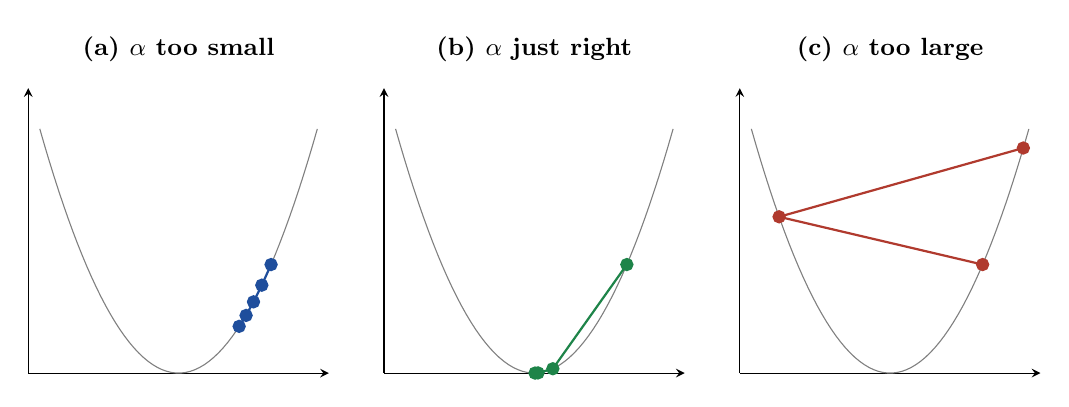
\begin{tikzpicture}
\begin{groupplot}[group style={group size=3 by 1,horizontal sep=0.7cm},width=5.4cm,height=5.2cm,
  xmin=-6.5,xmax=6.5,ymin=0,ymax=42,ticks=none,title style={font=\small\bfseries},axis lines=left]
\nextgroupplot[title={(a) $\alpha$ too small}]
\addplot[gray,domain=-6:6,samples=60]{x^2};
\addplot[mlblue,thick,mark=*,mark size=2pt] coordinates {(4,16)(3.6,12.96)(3.24,10.50)(2.92,8.50)(2.62,6.89)};
\nextgroupplot[title={(b) $\alpha$ just right}]
\addplot[gray,domain=-6:6,samples=60]{x^2};
\addplot[mlgreen,thick,mark=*,mark size=2pt] coordinates {(4,16)(0.8,0.64)(0.16,0.0256)(0.03,0.001)};
\nextgroupplot[title={(c) $\alpha$ too large}]
\addplot[gray,domain=-6:6,samples=60]{x^2};
\addplot[mlred,thick,mark=*,mark size=2pt] coordinates {(4,16)(-4.8,23.04)(5.76,33.18)};
\end{groupplot}
\end{tikzpicture}
\caption{Gradient descent on the loss $J(\theta)=\theta^2$ starting from $\theta=4$ with three learning rates.}\label{fig:gd}
\end{figure}

\begin{explain}
The grey bowl is a simple loss curve $J(\theta)=\theta^2$; the lowest point (the minimum) is at $\theta=0$. Each dot is one iteration, joined in order from the start at $\theta=4$. The update is $\theta\leftarrow\theta(1-2\alpha)$.\par
\textbf{(a) $\alpha=0.05$ (too small):} every step multiplies $\theta$ by $0.9$: safe, but after five steps we are still far from the bottom. Training is \emph{slow}.\par
\textbf{(b) $\alpha=0.4$ (good):} each step multiplies by $0.2$, and within three steps we are essentially at the minimum.\par
\textbf{(c) $\alpha=1.1$ (too large):} each step multiplies by $-1.2$, so we \emph{overshoot} the minimum and land higher on the opposite side each time: the loss \emph{increases} and the algorithm \textbf{diverges}.\par
\textbf{Lesson:} if the loss goes up, reduce the learning rate.
\end{explain}

\begin{center}
\begin{tabular}{@{}p{4.1cm}p{4.9cm}p{4.9cm}@{}}
\toprule
 & \textbf{Normal equation} & \textbf{Gradient descent}\\
\midrule
Learning rate $\alpha$ & Not needed & Must be chosen\\
Iterations & None (one formula) & Many\\
Many features ($d$ large) & Slow, $O(d^3)$ & Works well\\
Feature scaling & Not needed & \textbf{Needed} for fast convergence\\
Works for other models & No (linear regression only) & Yes (logistic regression, neural networks)\\
\bottomrule
\end{tabular}
\end{center}

\subsection{Multiple Linear Regression}

With $d$ features, $\hat y=\theta_0+\theta_1x_1+\cdots+\theta_dx_d=\vect\theta^{\!\top}\vect x$. Each coefficient $\theta_j$ is the change in $\hat y$ when $x_j$ increases by one unit \emph{while all other features are held fixed}.

\begin{example}[: House price]
A fitted model for house price (lakh Rs) is
\[
\widehat{\text{price}}=5+0.4\,(\text{area in m}^2)+6\,(\text{bedrooms})-0.5\,(\text{age in years}).
\]
For a house with 100~m$^2$, 3 bedrooms and 10 years old: $5+0.4(100)+6(3)-0.5(10)=5+40+18-5=\mathbf{58}$ lakh. Reading the coefficients: one extra bedroom adds 6 lakh and each year of age subtracts 0.5 lakh, other things equal.
\end{example}

\paragraph{Practical points.}
\begin{itemize}
  \item \textbf{Categorical features} (e.g.\ city) are converted to 0/1 \emph{dummy variables} (one-hot encoding).
  \item \textbf{Scale features} before gradient descent so that all weights learn at a similar speed.
  \item \textbf{Multicollinearity:} if two features are strongly correlated (area in m$^2$ and in ft$^2$) the coefficients become unstable. Drop one feature or use regularisation.
  \item \textbf{Polynomial regression:} adding $x^2,x^3,\dots$ as new features gives a \emph{curved} fit, yet the model is still \emph{linear in the parameters}, so all the theory applies. A high degree overfits (Chapter~2).
\end{itemize}

\subsection{Evaluating a Regression Model}

\begin{center}
\begin{tabular}{@{}p{3.1cm}p{5.1cm}p{5.6cm}@{}}
\toprule
\textbf{Metric} & \textbf{Formula} & \textbf{Meaning}\\
\midrule
MSE & $\frac1n\sum(y_i-\hat y_i)^2$ & Average squared error; punishes big errors\\
RMSE & $\sqrt{\text{MSE}}$ & Error in the \emph{units of $y$} (e.g.\ marks)\\
MAE & $\frac1n\sum|y_i-\hat y_i|$ & Average absolute error; robust to outliers\\
$R^2$ & $1-\dfrac{\text{SSE}}{\text{SST}}$ & Fraction of variance explained; 1 is perfect, 0 is no better than predicting $\bar y$\\
Adjusted $R^2$ & $1-(1-R^2)\dfrac{n-1}{n-p-1}$ & $R^2$ penalised for the number of features $p$\\
\bottomrule
\end{tabular}
\end{center}

For the marks example, $R^2=0.976$ and adjusted $R^2=1-0.0241\cdot\frac{4}{3}=0.968$.

\begin{warning}
A high $R^2$ on the \emph{training} data does not guarantee good predictions on new data. Always compute the metrics on a held-out test set. Also remember that \textbf{correlation is not causation}: studying more is associated with higher marks, but the regression alone cannot prove it causes them.
\end{warning}

\subsection{Regularised Linear Regression}

When there are many features, the least-squares weights can become large and overfit. \textbf{Regularisation} adds a penalty on the size of the weights:
\[
\text{Ridge (L2):}\ \ J(\vect\theta)+\lambda\sum_{j=1}^{d}\theta_j^2,\qquad
\text{Lasso (L1):}\ \ J(\vect\theta)+\lambda\sum_{j=1}^{d}|\theta_j| .
\]
\begin{itemize}
  \item \textbf{Ridge} shrinks all weights smoothly towards zero and handles correlated features well.
  \item \textbf{Lasso} can shrink some weights \emph{exactly to zero}, so it performs \textbf{automatic feature selection}.
  \item $\lambda\ge0$ is a hyperparameter (chosen by cross-validation): $\lambda=0$ gives ordinary least squares; large $\lambda$ gives an almost flat model (underfitting).
\end{itemize}

\begin{tryit}
Reproduce the hand results with \texttt{scikit-learn}:
\begin{lstlisting}
import numpy as np
from sklearn.linear_model import LinearRegression, Ridge

hours = np.array([[1], [2], [3], [4], [5]])
marks = np.array([35, 45, 50, 65, 70])

model = LinearRegression().fit(hours, marks)
print(model.intercept_, model.coef_[0])      # 26.0  9.0
print(model.predict([[6]]))                  # [80.]
print(model.score(hours, marks))             # R^2 = 0.9759

# regularised version: weights shrink a little
print(Ridge(alpha=1.0).fit(hours, marks).coef_)
\end{lstlisting}
\emph{Challenge:} add a student with 2 hours and 80 marks (an outlier). How do the slope and $R^2$ change?
\end{tryit}

%====================================================================
\procon{Linear regression}
{\item Simple, fast, easy to interpret (each coefficient is the effect of one feature)
 \item Needs little data
 \item A good baseline}
{\item Cannot capture non-linear relationships unless features are transformed
 \item Sensitive to outliers
 \item Affected by correlated features}
{\item House-price prediction
 \item Sales forecasting
 \item Estimating marks or salary
 \item Demand and risk modelling}

\section{Logistic Regression}


\begin{definition}[: Logistic regression]
\textbf{Logistic regression} is a \emph{supervised, parametric} method for \emph{classification}. It models the \textbf{probability} that an instance belongs to the positive class by passing a linear score through the \textbf{sigmoid} function, $P(y=1\mid\vect x)=\sigma(\vect w\cdot\vect x+b)=\dfrac{1}{1+e^{-(\vect w\cdot\vect x+b)}}$, and predicts class 1 if this probability exceeds a threshold (usually $0.5$). Despite its name it is a classification algorithm.
\end{definition}



\paragraph{Assumptions of logistic regression}
\begin{itemize}
  \item Binary (or categorical) target
  \item Independent observations
  \item Log-odds is a linear function of the features
  \item Little multicollinearity
  \item Enough data per class
\end{itemize}

\subsection{Why Not Use Linear Regression for Classes?}

Suppose we code ``fail $=0$, pass $=1$'' and fit a straight line. The line gives predictions like $-0.3$ or $1.4$, which are \emph{not valid probabilities}, and one extreme point can tilt the whole line. We need a function that squeezes any real number into $(0,1)$: the \textbf{sigmoid}.

\begin{definition}[: Sigmoid (logistic) function]
\[
  \sigma(z)=\frac{1}{1+e^{-z}},\qquad \sigma(0)=0.5,\qquad \sigma(-z)=1-\sigma(z),\qquad \sigma'(z)=\sigma(z)\big(1-\sigma(z)\big).
\]
\end{definition}

\begin{figure}[!htbp]
\centering
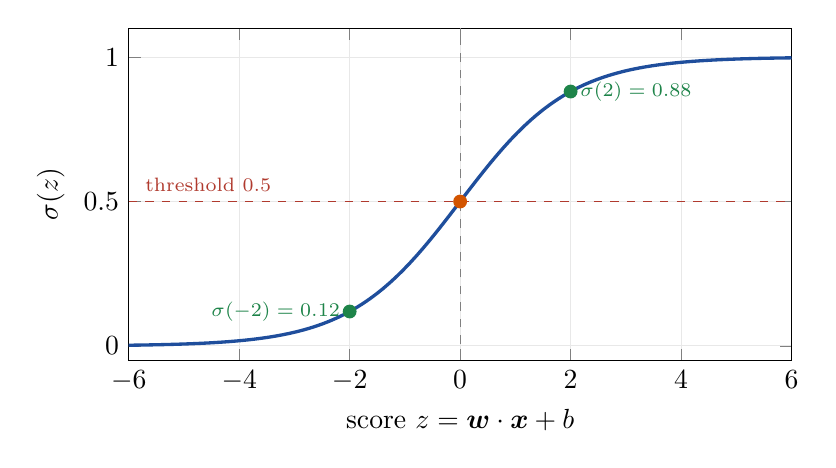
\begin{tikzpicture}
\begin{axis}[width=10cm,height=5.8cm,xlabel={score $z=\vect w\cdot\vect x+b$},ylabel={$\sigma(z)$},
  xmin=-6,xmax=6,ymin=-0.05,ymax=1.1,samples=100,grid=both,grid style={gray!18}]
\addplot[very thick,mlblue,domain=-6:6]{1/(1+exp(-x))};
\draw[dashed,mlred] (axis cs:-6,0.5)--(axis cs:6,0.5) node[pos=0.12,above,font=\scriptsize]{threshold $0.5$};
\draw[dashed,gray] (axis cs:0,-0.05)--(axis cs:0,1.1);
\fill[mlorange] (axis cs:0,0.5) circle (2.5pt);
\fill[mlgreen] (axis cs:2,0.8808) circle (2.5pt) node[right,font=\scriptsize]{$\sigma(2)=0.88$};
\fill[mlgreen] (axis cs:-2,0.1192) circle (2.5pt) node[left,font=\scriptsize]{$\sigma(-2)=0.12$};
\end{axis}
\end{tikzpicture}
\caption{The sigmoid function maps any real score to a probability between 0 and 1.}\label{fig:sigmoid}
\end{figure}

\begin{explain}
The horizontal axis is the \textbf{linear score} $z$ (which can be any real number) and the vertical axis is the \textbf{probability}. Large positive scores give probabilities near 1 (confident ``yes''); large negative scores give probabilities near 0 (confident ``no''). At $z=0$ the curve passes through $0.5$, the \textbf{decision threshold} (dashed red line): a score above 0 predicts class~1 and a score below 0 predicts class~0. The S-shape is steepest near $z=0$, where the model is least sure, and flat at the ends, where it is almost certain. The two green dots show the symmetry $\sigma(-2)=1-\sigma(2)$.
\end{explain}

\subsection{Odds and Log-odds}

\begin{definition}[: Odds and logit]
If an event has probability $p$, its \textbf{odds} are $\dfrac{p}{1-p}$ and its \textbf{log-odds (logit)} is $\ln\dfrac{p}{1-p}$.
\end{definition}

Logistic regression says that the \emph{log-odds is linear in the features}:
\[
  \ln\frac{p}{1-p}=\theta_0+\theta_1x_1+\cdots+\theta_dx_d .
\]
Hence $e^{\theta_j}$ is the \textbf{odds ratio}: the factor by which the odds are \emph{multiplied} when $x_j$ increases by one unit. For instance, if $p=0.8$ the odds are $0.8/0.2=4$ (``4 to 1''); if $p=0.5$ the odds are $1$.

\subsection{Loss Function: Cross-entropy from Maximum Likelihood}

For one example with label $y\in\{0,1\}$ and predicted probability $p=\sigma(z)$, the probability of the observed label is $p^{\,y}(1-p)^{1-y}$. Maximising the likelihood of all $n$ independent examples is the same as minimising the \textbf{cross-entropy (log) loss}
\begin{equation}\label{eq:logloss}
  J(\vect\theta)=-\frac1n\sum_{i=1}^{n}\Big[y_i\ln p_i+(1-y_i)\ln(1-p_i)\Big].
\end{equation}
\textbf{Why this loss?} If $y=1$ the loss is $-\ln p$: it is $0$ when $p=1$ and grows to $\infty$ as $p\to0$, so \emph{confident wrong answers are punished heavily}. There is no closed-form solution, so we use gradient descent. The gradient has the same neat form as in linear regression:
\[
  \frac{\partial J}{\partial\theta_j}=\frac1n\sum_{i=1}^{n}(p_i-y_i)\,x_{ij}.
\]

\begin{example}[: Computing the log-loss]
\begin{center}
\begin{tabular}{@{}cccl@{}}
\toprule
True $y$ & Predicted $p$ & Loss & Comment\\
\midrule
1 & 0.80 & $-\ln0.80=0.223$ & good\\
0 & 0.30 & $-\ln0.70=0.357$ & fairly good\\
1 & 0.10 & $-\ln0.10=2.303$ & confident and wrong: large loss\\
\bottomrule
\end{tabular}
\end{center}
Average of the first two: $(0.223+0.357)/2=0.290$.
\end{example}

\subsection{Real-life Example: Will the Student Pass?}

Twenty students record how many hours they studied and whether they passed. Training logistic regression by gradient descent (equivalently by \texttt{scikit-learn}) gives
\[
  z=-4.08+1.50\times\text{hours},\qquad P(\text{pass})=\sigma(z).
\]

\begin{example}[: End-to-end use of the trained model]
\textbf{(a) Probabilities.} $P(\text{pass})=\sigma(-4.08+1.50\,h)$:
\begin{center}
\begin{tabular}{@{}c|ccccc@{}}
\toprule
Hours $h$ & 1 & 2 & 3 & 4 & 5\\
Score $z$ & $-2.58$ & $-1.08$ & $0.42$ & $1.92$ & $3.42$\\
$P(\text{pass})=\frac{1}{1+e^{-z}}$ & 0.070 & 0.254 & 0.604 & 0.872 & 0.968\\
Prediction ($\ge0.5$) & Fail & Fail & Pass & Pass & Pass\\
\bottomrule
\end{tabular}
\end{center}
For $h=3$: $e^{-0.42}=0.657$, so $P=\dfrac{1}{1+0.657}=0.604$.\par
\textbf{(b) Decision boundary.} $P=0.5\iff z=0\iff h=\dfrac{4.08}{1.50}=\mathbf{2.72}$ hours: students who study more than about 2.7 hours are predicted to pass.\par
\textbf{(c) Meaning of the coefficient.} The odds ratio is $e^{1.50}=4.48$: each extra hour of study multiplies the odds of passing by about \textbf{4.5}. (At $h=2$ the odds are $0.254/0.746=0.34$; at $h=3$ they are $0.604/0.396=1.52$; and $1.52/0.34\approx4.5$.)\par
\textbf{(d) Accuracy.} Using the 0.5 rule on the 20 training students: 10 students studied less than 2.72 h (predicted Fail; 8 really failed, 2 passed) and 10 studied more (predicted Pass; 8 passed, 2 failed). So
\begin{center}
\begin{tabular}{@{}cc|cc@{}}
\toprule
 & & \multicolumn{2}{c}{Predicted}\\
 & & Pass & Fail\\
\midrule
\multirow{2}{*}{Actual} & Pass & $TP=8$ & $FN=2$\\
 & Fail & $FP=2$ & $TN=8$\\
\bottomrule
\end{tabular}
\end{center}
Accuracy $=16/20=0.80$, precision $=8/10=0.80$, recall $=8/10=0.80$ (formulas of Chapter~2).
\end{example}

\begin{figure}[!htbp]
\centering
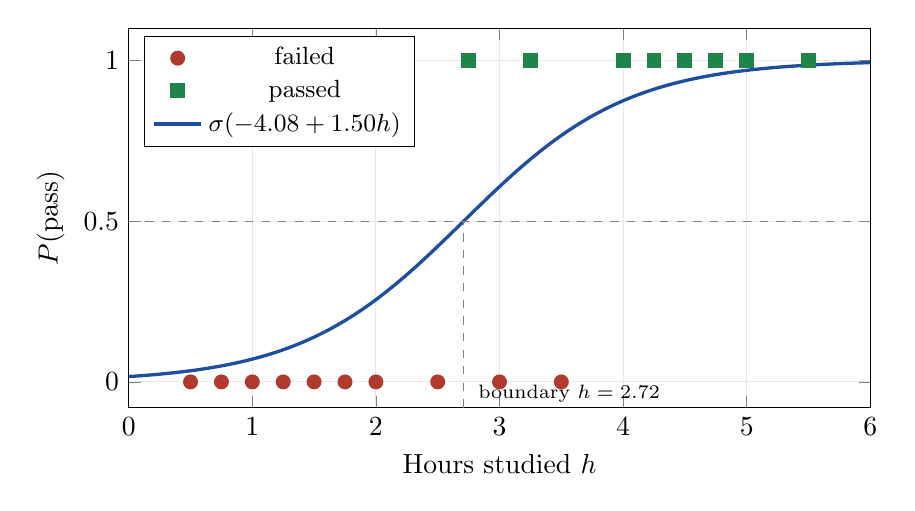
\begin{tikzpicture}
\begin{axis}[width=11cm,height=6.4cm,xlabel={Hours studied $h$},ylabel={$P(\text{pass})$},
  xmin=0,xmax=6,ymin=-0.08,ymax=1.1,samples=100,grid=both,grid style={gray!18},
  legend style={at={(0.02,0.98)},anchor=north west,font=\small}]
\addplot[only marks,mark=*,mlred,mark size=2.5pt] coordinates {(0.5,0)(0.75,0)(1,0)(1.25,0)(1.5,0)(1.75,0)(2,0)(2.5,0)(3,0)(3.5,0)};
\addlegendentry{failed}
\addplot[only marks,mark=square*,mlgreen,mark size=2.5pt] coordinates {(1.75,1)(2.25,1)(2.75,1)(3.25,1)(4,1)(4.25,1)(4.5,1)(4.75,1)(5,1)(5.5,1)};
\addlegendentry{passed}
\addplot[very thick,mlblue,domain=0:6]{1/(1+exp(-(-4.0787+1.505*x)))};
\addlegendentry{$\sigma(-4.08+1.50h)$}
\draw[dashed,gray] (axis cs:0,0.5)--(axis cs:6,0.5);
\draw[dashed,gray] (axis cs:2.71,-0.08)--(axis cs:2.71,0.5);
\node[font=\scriptsize,anchor=north west] at (axis cs:2.75,0.02) {boundary $h=2.72$};
\end{axis}
\end{tikzpicture}
\caption{Logistic regression fitted to 20 students: the S-curve is the predicted probability of passing.}\label{fig:logfit}
\end{figure}

\begin{explain}
Red dots at height 0 are students who \textbf{failed}; green squares at height 1 are students who \textbf{passed}. The \textbf{blue S-curve} is the model's predicted probability of passing for any number of study hours. It rises slowly at first, climbs quickly around 2--3.5 hours and flattens near 1. Where the curve crosses the horizontal dashed line (probability $0.5$), the vertical dashed line marks the \textbf{decision boundary} at about 2.7 hours. Note the overlap: some students who studied about 2--3 hours passed and others failed, so the model is naturally \emph{uncertain} there and the curve gives a probability, not a hard yes/no. A straight regression line through these 0/1 points would go below 0 and above 1, which makes no sense for probabilities.
\end{explain}

\subsection{Training by Gradient Descent: One Step by Hand}

\begin{example}[: One gradient step of logistic regression]
Five students: $x=(1,2,3,4,5)$ hours and $y=(0,0,1,0,1)$. Start with $\theta_0=\theta_1=0$, so $z=0$ and $p=\sigma(0)=0.5$ for everyone. Use $\alpha=0.5$.\par
Errors $p-y=(0.5,\ 0.5,\ -0.5,\ 0.5,\ -0.5)$.
\[
\tfrac{\partial J}{\partial\theta_0}=\tfrac{0.5+0.5-0.5+0.5-0.5}{5}=0.1,\qquad
\tfrac{\partial J}{\partial\theta_1}=\tfrac{0.5(1)+0.5(2)-0.5(3)+0.5(4)-0.5(5)}{5}=\tfrac{-0.5}{5}=-0.1 .
\]
\[
\theta_0=0-0.5(0.1)=-0.05,\qquad \theta_1=0-0.5(-0.1)=0.05 .
\]
The new score is $z=-0.05+0.05x$; the 5-hour student now gets $\sigma(0.20)=0.55$ instead of $0.50$. Repeating the step many times converges to the best weights.
\end{example}

\subsection{Multiclass Logistic Regression}

For $K>2$ classes there are two standard approaches.
\begin{itemize}
  \item \textbf{One-vs-Rest (OvR):} train $K$ binary classifiers (``class $k$ vs.\ all others'') and pick the class with the highest probability.
  \item \textbf{Softmax (multinomial) regression:} compute a score $z_k$ for each class and convert them to probabilities that sum to 1,
  \[
    P(y=k\mid\vect x)=\frac{e^{z_k}}{\sum_{j=1}^{K}e^{z_j}} .
  \]
\end{itemize}

\begin{example}[: Softmax]
Scores $z=(2.0,\ 1.0,\ 0.1)$ for three classes: $e^{z}=(7.389,\ 2.718,\ 1.105)$, sum $=11.212$, so the probabilities are $(0.659,\ 0.242,\ 0.099)$ and the predicted class is the first.
\end{example}

\subsection{Choosing the Threshold and Regularisation}

\begin{itemize}
  \item The threshold $0.5$ is not sacred. For \emph{cancer screening} a missed patient (false negative) is very costly, so we lower the threshold (say to $0.2$) to raise \textbf{recall}, accepting more false alarms. For \emph{spam filtering} a good mail sent to spam (false positive) is costly, so we raise it to improve \textbf{precision}.
  \item Logistic regression can be \textbf{regularised} just like linear regression (L2 or L1 penalty). In \texttt{scikit-learn} the parameter \texttt{C} is the \emph{inverse} of regularisation strength: smaller \texttt{C} means stronger regularisation.
\end{itemize}

\begin{center}
\begin{tabular}{@{}p{3.5cm}p{4.9cm}p{4.9cm}@{}}
\toprule
 & \textbf{Linear regression} & \textbf{Logistic regression}\\
\midrule
Task & Regression (predict a number) & Classification (predict a class / probability)\\
Output & Any real value & Probability in $(0,1)$\\
Function & $\hat y=\vect\theta^{\!\top}\vect x$ & $\hat p=\sigma(\vect\theta^{\!\top}\vect x)$\\
Loss & Squared error & Cross-entropy (log loss)\\
Solution & Closed form or gradient descent & Gradient descent only\\
Metric & MSE, RMSE, $R^2$ & Accuracy, precision, recall, $F_1$, log-loss\\
Example & Marks from study hours & Pass/fail from study hours\\
\bottomrule
\end{tabular}
\end{center}

\begin{tryit}
Reproduce the pass/fail model:
\begin{lstlisting}
import numpy as np
from sklearn.linear_model import LogisticRegression

h = np.array([.5,.75,1,1.25,1.5,1.75,1.75,2,2.25,2.5,
              2.75,3,3.25,3.5,4,4.25,4.5,4.75,5,5.5]).reshape(-1, 1)
p = np.array([0,0,0,0,0,0,1,0,1,0, 1,0,1,0,1,1,1,1,1,1])

# a very large C = almost no regularisation
clf = LogisticRegression(C=1e6).fit(h, p)
print(clf.intercept_, clf.coef_)           # about -4.08  1.50
print(clf.predict_proba([[3]])[0, 1])      # P(pass | 3 h) = 0.607
print(clf.score(h, p))                     # accuracy = 0.80
\end{lstlisting}
Fitted coefficients: intercept $-4.079$, slope $1.505$, boundary at $2.71$ hours, training accuracy $0.80$, matching the hand calculation. \emph{Challenge:} predict the probabilities for 1, 2, 4 and 5 hours (answer: $0.07,\ 0.26,\ 0.88,\ 0.97$).
\end{tryit}

%====================================================================
\procon{Logistic regression}
{\item Gives \emph{probabilities}, not only labels
 \item Simple, fast and interpretable (coefficients are log-odds ratios)
 \item Linear decision boundary
 \item Works well as a baseline
 \item Can be regularised}
{\item Only linear boundaries unless features are transformed
 \item May underperform on complex data
 \item Sensitive to outliers and correlated features
 \item Fails on perfectly separable data without regularisation}
{\item Spam detection
 \item Disease diagnosis
 \item Loan default
 \item Customer churn
 \item Pass/fail prediction}

\section{Generalized Linear Models (GLMs)}


\begin{definition}[: Generalized linear model (GLM)]
A \textbf{generalized linear model (GLM)} is a flexible extension of linear regression that allows the response $y$ to follow any distribution from the \textbf{exponential family} (normal, Bernoulli/binomial, Poisson, gamma, \dots) and relates its \textbf{mean} $\mu=\E[y\mid\vect x]$ to a linear predictor through a \textbf{link function}: $g(\mu)=\vect\theta^{\!\top}\vect x$.
\end{definition}



\paragraph{The three components of a GLM}
\begin{enumerate}
  \item \emph{Random component:} the distribution of $y$ (exponential family).
  \item \emph{Systematic component:} the linear predictor $\eta=\theta_0+\theta_1x_1+\cdots+\theta_dx_d$.
  \item \emph{Link function:} $g$, with $g(\mu)=\eta$, i.e.\ $\mu=g^{-1}(\eta)$
\end{enumerate}

\begin{figure}[!htbp]
\centering
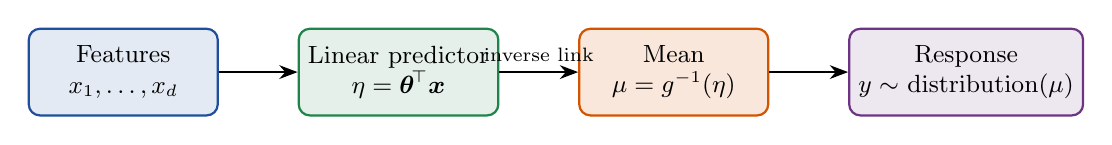
\begin{tikzpicture}[node distance=1.0cm,
  b/.style={draw,rounded corners,thick,align=center,font=\small,minimum height=1.1cm,minimum width=2.4cm},
  arr/.style={-{Stealth},thick}]
\node[b,fill=mlblue!12,draw=mlblue] (x) {Features\\$x_1,\dots,x_d$};
\node[b,fill=mlgreen!12,draw=mlgreen,right=of x] (eta) {Linear predictor\\$\eta=\vect\theta^{\!\top}\vect x$};
\node[b,fill=mlorange!14,draw=mlorange,right=of eta] (mu) {Mean\\$\mu=g^{-1}(\eta)$};
\node[b,fill=mlpurple!12,draw=mlpurple,right=of mu] (y) {Response\\$y\sim$ distribution$(\mu)$};
\draw[arr] (x)--(eta); \draw[arr] (eta)--(mu) node[midway,above,font=\scriptsize]{inverse link}; \draw[arr] (mu)--(y);
\end{tikzpicture}
\caption{Structure of a generalized linear model.}\label{fig:glm}
\end{figure}

\begin{explain}
Read left to right. The \textbf{features} are combined linearly into a score $\eta$ (green box), exactly as in linear regression. The \textbf{inverse link} $g^{-1}$ (arrow label) then converts this unbounded score into the \textbf{mean} $\mu$ of the response, forcing it into a sensible range (for example $(0,1)$ for probabilities or $(0,\infty)$ for counts). Finally the \textbf{actual outcome} $y$ is a random draw from a distribution (normal, Bernoulli, Poisson, \dots) whose mean is $\mu$. Changing the \emph{link} and the \emph{distribution} gives different models: this single picture covers linear, logistic and Poisson regression.
\end{explain}

\begin{center}
\begin{tabular}{@{}p{3.1cm}p{2.7cm}p{2.7cm}p{2.5cm}p{2.6cm}@{}}
\toprule
\textbf{Model} & \textbf{Distribution of $y$} & \textbf{Link $g(\mu)$} & \textbf{Mean $\mu$} & \textbf{Target type}\\
\midrule
Linear regression & Normal & identity: $\mu$ & $\eta$ & real number\\
Logistic regression & Bernoulli & logit: $\ln\frac{\mu}{1-\mu}$ & $\frac1{1+e^{-\eta}}$ & 0/1 class\\
Poisson regression & Poisson & log: $\ln\mu$ & $e^{\eta}$ & count $0,1,2,\dots$\\
Gamma regression & Gamma & inverse: $1/\mu$ & $1/\eta$ & positive, skewed\\
\bottomrule
\end{tabular}
\end{center}

\begin{keyidea}
\textbf{Linear regression and logistic regression are both GLMs.} Linear regression uses a Normal distribution with the identity link; logistic regression uses a Bernoulli distribution with the logit link. This is why they share the same gradient formula $\frac1n\sum(\hat\mu_i-y_i)x_{ij}$.
\end{keyidea}

\subsection{Real-life Example: Poisson Regression for Emergency Calls}

A city fire-control room counts the number of emergency calls per day. The count depends on the rainfall $x$ (mm): $y\sim\text{Poisson}(\mu)$ with
\[
  \ln\mu=1+0.2\,x\qquad\Longleftrightarrow\qquad\mu=e^{\,1+0.2x}.
\]

\begin{example}[: Using the model]
\textbf{Expected calls on a dry day} ($x=0$): $\mu=e^{1}=2.72$.\par
\textbf{On a day with 5 mm rain:} $\mu=e^{1+1.0}=e^{2}=7.39$ calls.\par
\textbf{On a day with 10 mm rain:} $\mu=e^{3}=20.09$ calls.\par
\textbf{Interpretation of the coefficient:} each extra millimetre of rain multiplies the expected number of calls by $e^{0.2}=1.22$, i.e.\ an increase of about \textbf{22\%} per mm. Notice that the prediction is always positive, which an ordinary linear model could not guarantee.\par
\textbf{Probability of exactly 7 calls on the 5 mm day:} for a Poisson variable $P(y=k)=\dfrac{\mu^ke^{-\mu}}{k!}$, so $P(y=7)=\dfrac{7.39^{7}e^{-7.39}}{5040}\approx0.15$.
\end{example}

%====================================================================
\procon{Generalized linear models}
{\item One unified framework
 \item Handles counts, proportions and binary data properly
 \item Predictions always stay in the valid range
 \item Coefficients remain interpretable}
{\item Still assumes a linear relationship on the link scale
 \item Sensitive to outliers
 \item The distribution must be chosen correctly (e.g.\ over-dispersed counts break the Poisson model)}
{\item Insurance claim counts
 \item Accident/call counts
 \item Binary outcomes (credit default)
 \item Proportions
 \item Waiting times}

\section{Binary Classification and Support Vector Machines}

\subsection{Binary Classification}

\begin{definition}[: Binary classification]
\textbf{Binary classification} is the supervised task of assigning each input to one of exactly \textbf{two classes}, called the \textbf{positive} and \textbf{negative} class (coded $\{0,1\}$ in logistic regression or $\{-1,+1\}$ in SVMs). The classifier learns a \textbf{decision function} $f(\vect x)$ and predicts the positive class when $f(\vect x)$ exceeds a threshold.
\end{definition}

A \textbf{linear classifier} uses $f(\vect x)=\vect w\cdot\vect x+b$; the set $\{\vect x:\vect w\cdot\vect x+b=0\}$ is a \textbf{hyperplane} (a line in 2-D, a plane in 3-D) that cuts the space into the two decision regions. \textbf{Examples:} spam / not spam, fraud / genuine, disease / healthy, loan default / repay. Performance is judged with the confusion matrix, precision, recall, $F_1$ (Chapter~2) and the \textbf{ROC curve} (true-positive rate against false-positive rate for all thresholds; the area under it, \textbf{AUC}, is $1$ for a perfect classifier and $0.5$ for random guessing).

\begin{warning}
Many different lines can separate the same two classes perfectly. Which one is \emph{best}? Logistic regression picks the one with the best likelihood; the \textbf{SVM} picks the one \textbf{farthest from both classes}, which tends to generalise better.
\end{warning}

\subsection{The Support Vector Machine (Linear, Hard Margin)}


\begin{definition}[: Support vector machine (hard margin)]
A \textbf{Support Vector Machine (SVM)} is a \emph{supervised} learning algorithm for \emph{classification} (and regression) that finds the \textbf{maximum-margin hyperplane}: the separating hyperplane $\vect w\cdot\vect x+b=0$ that is \textbf{as far as possible from the nearest training points of both classes}. The nearest points that fix the boundary are called \textbf{support vectors}.
\end{definition}



\paragraph{Geometry.} The distance from a point $\vect x_0$ to the hyperplane $\vect w\cdot\vect x+b=0$ is $\dfrac{|\vect w\cdot\vect x_0+b|}{\|\vect w\|}$. We scale $\vect w,b$ so that the closest points satisfy $|\vect w\cdot\vect x+b|=1$. Then the two \emph{margin lines} are $\vect w\cdot\vect x+b=+1$ and $\vect w\cdot\vect x+b=-1$ and the \textbf{margin width} is
\[
  \frac{1}{\|\vect w\|}+\frac{1}{\|\vect w\|}=\frac{2}{\|\vect w\|}.
\]
Making the margin wide means making $\|\vect w\|$ small. The \textbf{hard-margin SVM} is therefore the optimisation problem
\begin{equation}\label{eq:svm}
  \min_{\vect w,b}\ \tfrac12\|\vect w\|^2\qquad\text{subject to}\qquad y_i\,(\vect w\cdot\vect x_i+b)\ \ge\ 1\quad\text{for all }i .
\end{equation}

\begin{figure}[!htbp]
\centering
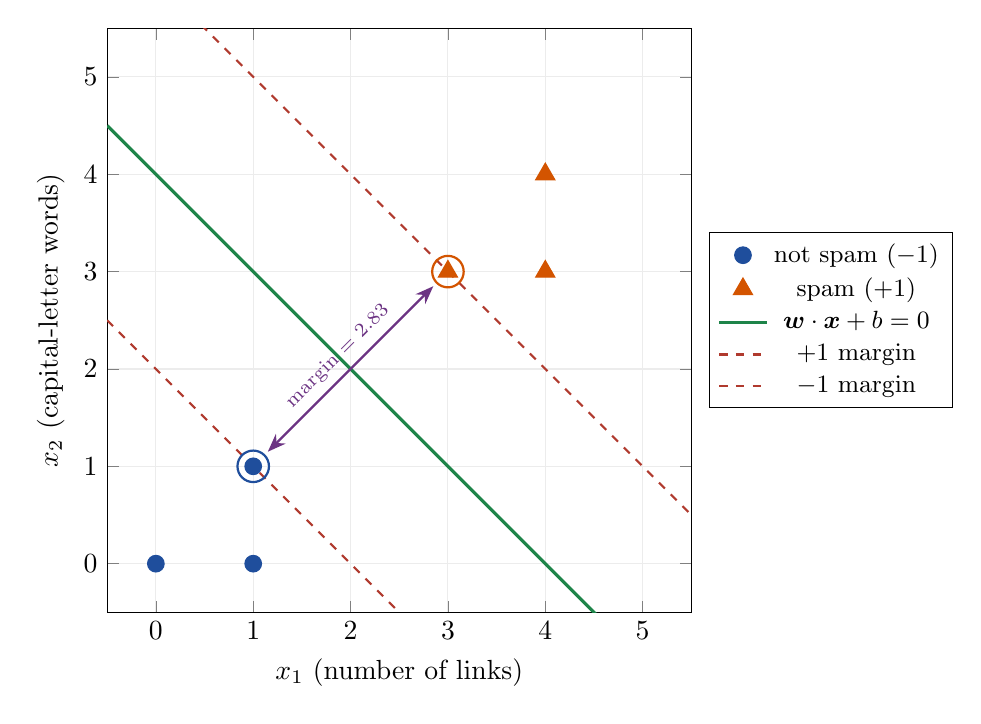
\begin{tikzpicture}
\begin{axis}[width=9cm,height=9cm,xmin=-0.5,xmax=5.5,ymin=-0.5,ymax=5.5,axis equal image,
  xlabel={$x_1$ (number of links)},ylabel={$x_2$ (capital-letter words)},grid=both,grid style={gray!15},
  legend style={at={(1.03,0.5)},anchor=west,font=\small}]
\addplot[only marks,mark=*,mlblue,mark size=3pt] coordinates {(1,1)(0,0)(1,0)};
\addlegendentry{not spam ($-1$)}
\addplot[only marks,mark=triangle*,mlorange,mark size=4pt] coordinates {(3,3)(4,4)(4,3)};
\addlegendentry{spam ($+1$)}
\addplot[very thick,mlgreen,domain=-0.5:5.5]{4-x};
\addlegendentry{$\vect w\cdot\vect x+b=0$}
\addplot[dashed,mlred,thick,domain=-0.5:5.5]{6-x};
\addlegendentry{$+1$ margin}
\addplot[dashed,mlred,thick,domain=-0.5:5.5]{2-x};
\addlegendentry{$-1$ margin}
\draw[mlblue,thick] (axis cs:1,1) circle (0.2cm);
\draw[mlorange,thick] (axis cs:3,3) circle (0.2cm);
\draw[{Stealth}-{Stealth},thick,mlpurple] (axis cs:1.15,1.15)--(axis cs:2.85,2.85);
\node[font=\scriptsize,mlpurple,rotate=45,above] at (axis cs:2.0,2.0) {margin $=2.83$};
\end{axis}
\end{tikzpicture}
\caption{Maximum-margin separation of spam and non-spam e-mails. Circled points are the support vectors.}\label{fig:svm}
\end{figure}

\begin{explain}
Each point is an e-mail described by two features. The \textbf{solid green line} is the decision boundary. The two \textbf{dashed red lines} are the \textbf{margin}: they pass through the nearest point of each class, the \textbf{circled support vectors} $(1,1)$ and $(3,3)$. The \textbf{purple arrow} is the margin width, the gap that the SVM tries to make as large as possible. Only the circled points decide where the line goes. If you moved or deleted the other four points (without crossing the margin), the boundary would \emph{not change}. A different separating line (say, tilted) could also split the classes, but it would pass closer to some points and generalise worse.
\end{explain}

\begin{example}[: SVM by hand on the spam data]
\textbf{Data.} Three non-spam mails (class $-1$): $(1,1),\ (0,0),\ (1,0)$. Three spam mails (class $+1$): $(3,3),\ (4,4),\ (4,3)$. Features: number of links $x_1$ and number of words in capitals $x_2$.\par
\textbf{Step 1: find the closest opposite pair.} The nearest points are $(1,1)$ and $(3,3)$ (distance $\sqrt{8}=2.83$). They are the support vectors; by symmetry the boundary passes midway, perpendicular to the line joining them, so $\vect w=(a,a)$.\par
\textbf{Step 2: impose the margin conditions.}
\[
\vect w\cdot(3,3)+b=+1\ \Rightarrow\ 6a+b=1,\qquad
\vect w\cdot(1,1)+b=-1\ \Rightarrow\ 2a+b=-1 .
\]
Subtracting: $4a=2\Rightarrow a=0.5$; then $b=-1-2(0.5)=-2$. So $\vect w=(0.5,\,0.5)$, $b=-2$ and the boundary is $0.5x_1+0.5x_2-2=0$, i.e.\ $\ x_1+x_2=4$.\par
\textbf{Step 3: verify all six constraints} $y_i(\vect w\cdot\vect x_i+b)\ge1$:
\begin{center}
\begin{tabular}{@{}c|cccccc@{}}
\toprule
Point & $(1,1)$ & $(0,0)$ & $(1,0)$ & $(3,3)$ & $(4,4)$ & $(4,3)$\\
$f=0.5x_1+0.5x_2-2$ & $-1$ & $-2$ & $-1.5$ & $1$ & $2$ & $1.5$\\
$y\,f$ & 1 & 2 & 1.5 & 1 & 2 & 1.5\\
Satisfied? & on margin & yes & yes & on margin & yes & yes\\
\bottomrule
\end{tabular}
\end{center}
All $y_if(\vect x_i)\ge1$, and exactly two points equal $1$: they are the support vectors.\par
\textbf{Step 4: margin.} $\|\vect w\|=\sqrt{0.25+0.25}=0.707$, so the margin is $2/0.707=\mathbf{2.83}$.\par
\textbf{Step 5: predict.} A new mail with 4 links and 1 capital word: $f=0.5(4)+0.5(1)-2=0.5>0\Rightarrow$ \textbf{spam}. A mail with $(1,2)$: $f=0.5+1-2=-0.5<0\Rightarrow$ \textbf{not spam}.
\end{example}

\subsection{Soft-Margin SVM}

Real data usually overlap, so no hyperplane separates the classes perfectly (and noisy points would make a hard margin very narrow). The \textbf{soft-margin SVM} allows some points to violate the margin by introducing \textbf{slack variables} $\xi_i\ge0$:
\begin{equation}\label{eq:softsvm}
  \min_{\vect w,b,\vect\xi}\ \tfrac12\|\vect w\|^2+C\sum_{i=1}^{n}\xi_i\qquad\text{subject to}\qquad y_i(\vect w\cdot\vect x_i+b)\ge1-\xi_i,\ \ \xi_i\ge0 .
\end{equation}
Here $\xi_i=0$ for a correctly classified point outside the margin, $0<\xi_i\le1$ for a point inside the margin but on the correct side, and $\xi_i>1$ for a misclassified point. The hyperparameter $C$ controls the trade-off:

\begin{center}
\begin{tabular}{@{}p{3.4cm}p{4.9cm}p{4.9cm}@{}}
\toprule
 & \textbf{Large $C$} & \textbf{Small $C$}\\
\midrule
Priority & Few training errors & Wide margin\\
Margin & Narrow & Wide\\
Bias / variance & Low bias, high variance & Higher bias, lower variance\\
Risk & Overfitting & Underfitting\\
\bottomrule
\end{tabular}
\end{center}

Equivalently, the soft-margin SVM minimises the \textbf{hinge loss}
\[
  L_{\text{hinge}}=\max\big(0,\ 1-y\,f(\vect x)\big),
\]
which is $0$ for points correctly classified \emph{beyond} the margin and grows linearly otherwise. For example, with $y=+1$: $f=2\Rightarrow$ loss $0$; $f=0.3\Rightarrow0.7$; $f=-0.5\Rightarrow1.5$.

\begin{figure}[!htbp]
\centering
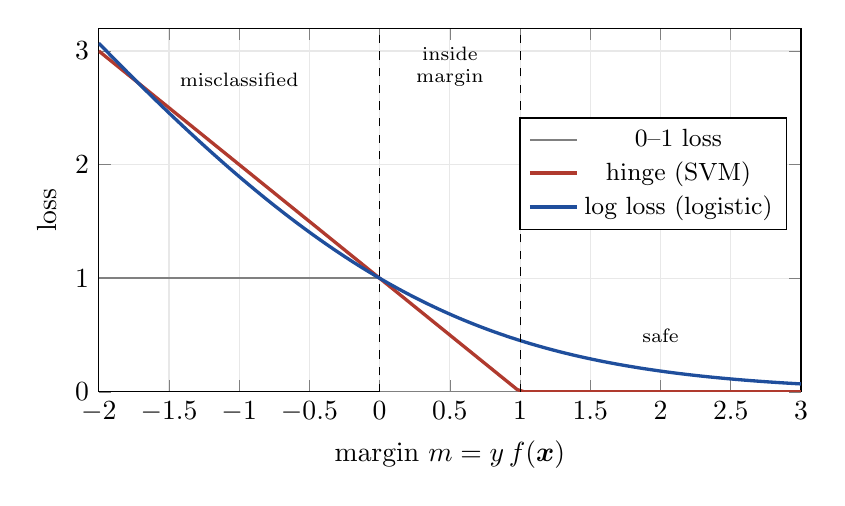
\begin{tikzpicture}
\begin{axis}[width=10.5cm,height=6.2cm,xlabel={margin $m=y\,f(\vect x)$},ylabel={loss},
  xmin=-2,xmax=3,ymin=0,ymax=3.2,samples=100,grid=both,grid style={gray!18},
  legend style={at={(0.98,0.60)},anchor=east,font=\small}]
\addplot[thick,gray,domain=-2:-0.001]{1};
\addplot[thick,gray,domain=0.001:3,forget plot]{0};
\addlegendentry{0--1 loss}
\addplot[very thick,mlred,domain=-2:3]{max(0,1-x)};
\addlegendentry{hinge (SVM)}
\addplot[very thick,mlblue,domain=-2:3]{ln(1+exp(-x))/ln(2)};
\addlegendentry{log loss (logistic)}
\draw[dashed] (axis cs:0,0)--(axis cs:0,3.2);
\draw[dashed] (axis cs:1,0)--(axis cs:1,3.2);
\node[font=\scriptsize,anchor=south] at (axis cs:-1,2.6) {misclassified};
\node[font=\scriptsize,anchor=south] at (axis cs:2,0.35) {safe};
\node[font=\scriptsize,anchor=south,align=center] at (axis cs:0.5,2.6) {inside\\margin};
\end{axis}
\end{tikzpicture}
\caption{Loss as a function of the margin $m=y\,f(\vect x)$: 0--1 loss, hinge loss (SVM) and log loss (logistic regression).}\label{fig:losses}
\end{figure}

\begin{explain}
The horizontal axis is the \textbf{margin} $m=y\,f(\vect x)$: it is positive when the point is on the \emph{correct} side and negative when on the \emph{wrong} side, and bigger values mean greater confidence. \textbf{Grey (0--1 loss):} counts a mistake as 1 and a correct answer as 0, but it is a cliff, so we cannot use gradients on it. \textbf{Red (hinge loss):} zero once $m\ge1$ (``correct with room to spare''), so points beyond the margin contribute \emph{nothing}, and grows linearly for $m<1$, including points that are right but inside the margin. \textbf{Blue (log loss):} never exactly zero, so every point still matters a little, and it decreases smoothly. Both red and blue curves are smooth-ish \emph{upper bounds} on the 0--1 loss that can be optimised. This single picture shows why an SVM depends only on a few support vectors, while logistic regression uses all points.
\end{explain}

\begin{keyidea}
\textbf{SVM vs logistic regression.} Both learn a linear boundary. Logistic regression minimises the log loss and outputs \emph{probabilities}; the SVM minimises the hinge loss and maximises the \emph{margin}, depending only on the support vectors. When classes are nearly separable the SVM often generalises slightly better; when you need probabilities, use logistic regression. The \emph{kernel trick} that lets SVMs learn \emph{non-linear} boundaries is covered in Chapter~6.
\end{keyidea}

\begin{tryit}
Verify the hand-solved SVM:
\begin{lstlisting}
import numpy as np
from sklearn.svm import SVC

X = np.array([[1,1],[0,0],[1,0],[3,3],[4,4],[4,3]])   # [links, capitals]
y = np.array([-1,-1,-1, 1, 1, 1])                      # -1 ham, +1 spam

svm = SVC(kernel="linear", C=1e6).fit(X, y)   # huge C = hard margin
print(svm.coef_, svm.intercept_)       # [[0.5 0.5]] [-2.]
print(svm.support_vectors_)            # [[1. 1.] [3. 3.]]
print(svm.predict([[4, 1]]))           # [1]  -> spam
print(svm.decision_function([[4, 1]])) # [0.5]
\end{lstlisting}
The output reproduces $\vect w=(0.5,0.5)$, $b=-2$, the two support vectors and $f(4,1)=0.5$. \emph{Challenge:} set \texttt{C=0.01} and watch what happens to the margin and the support vectors.
\end{tryit}

%====================================================================
\procon{Support vector machines}
{\item Effective in high dimensions
 \item Only the support vectors matter, so it is memory-efficient
 \item Strong generalisation because of the maximum margin
 \item Flexible through kernels}
{\item Slow on very large datasets
 \item Requires feature scaling
 \item Sensitive to the choice of $C$ and the kernel
 \item Does not directly output probabilities
 \item Hard to interpret with non-linear kernels}
{\item Text and spam classification
 \item Image and face recognition
 \item Handwriting recognition
 \item Bioinformatics (gene and protein classification)}

\section{Choosing Among the Methods of Unit II}

\begin{center}
\small
\begin{tabular}{@{}p{2.7cm}p{2.6cm}p{2.8cm}p{2.7cm}p{2.7cm}@{}}
\toprule
 & \textbf{k-NN} & \textbf{Decision tree} & \textbf{Naive Bayes} & \textbf{Linear / Logistic / SVM}\\
\midrule
Boundary & Irregular, local & Axis-parallel boxes & Smooth (probabilistic) & Linear hyperplane\\
Interpretable? & Low & High & Moderate & High (coefficients)\\
Needs scaling? & Yes & No & No & Yes\\
Training speed & None & Fast & Very fast & Fast--moderate\\
Outputs probabilities? & Roughly & Roughly & Yes & Logistic: yes; SVM: no\\
Good when & Small data, local patterns & Mixed features, rules needed & Text, little data & Many features, linear structure\\
\bottomrule
\end{tabular}
\end{center}

%====================================================================
\begin{summary}
\begin{itemize}
  \item \textbf{Linear regression:} $\hat y=\vect\theta^{\!\top}\vect x$, fitted by least squares: $\theta_1=S_{xy}/S_{xx}$, $\theta_0=\bar y-\theta_1\bar x$, or $\vect\theta=(\mathbf X^{\!\top}\mathbf X)^{-1}\mathbf X^{\!\top}\vect y$, or gradient descent $\theta_j\leftarrow\theta_j-\alpha\,\partial J/\partial\theta_j$. Evaluate with MSE, RMSE, $R^2$. Ridge (L2) and Lasso (L1) regularise.
  \item \textbf{Logistic regression:} $P(y=1)=\sigma(\vect\theta^{\!\top}\vect x)$; log-odds is linear; trained by minimising cross-entropy (maximum likelihood); predicts class 1 if $p\ge0.5$; $e^{\theta_j}$ is the odds ratio. Softmax extends it to many classes.
  \item \textbf{GLM:} distribution from the exponential family $+$ linear predictor $+$ link function $g(\mu)=\eta$. Linear (identity), logistic (logit) and Poisson (log) regression are special cases.
  \item \textbf{Binary classification:} two classes, decision function and hyperplane; evaluate with confusion matrix, precision, recall, $F_1$, ROC--AUC.
  \item \textbf{SVM:} maximum-margin hyperplane; margin $=2/\|\vect w\|$; minimise $\frac12\|\vect w\|^2$ s.t.\ $y_i(\vect w\cdot\vect x_i+b)\ge1$; only \textbf{support vectors} matter; soft margin adds slack and $C$; hinge loss $\max(0,1-yf)$.
  \item Worked examples: marks $=26+9\times$hours ($R^2=0.976$); pass probability $\sigma(-4.08+1.5h)$ with boundary $2.72$ h; Poisson calls $e^{1+0.2x}$; SVM $\vect w=(0.5,0.5)$, $b=-2$, margin $2.83$.
\end{itemize}
\end{summary}

%====================================================================
\section*{Exam Corner}
\addcontentsline{toc}{section}{Exam Corner}

\subsection*{A.\ Very Short Answer Questions (2 marks each)}
\begin{enumerate}
  \item Define linear regression. \qmarks{2}
  \item What is a residual? What does the method of least squares minimise? \qmarks{2}
  \item Write the gradient-descent update rule. What is the role of the learning rate? \qmarks{2}
  \item Define $R^2$. What does $R^2=0.9$ mean? \qmarks{2}
  \item Differentiate Ridge and Lasso regression. \qmarks{2}
  \item Define the sigmoid function. What is its range? \qmarks{2}
  \item Define odds and log-odds. \qmarks{2}
  \item Why is logistic regression a classification algorithm even though it has ``regression'' in its name? \qmarks{2}
  \item Define a generalized linear model. What is a link function? \qmarks{2}
  \item What are support vectors? What is the margin of an SVM? \qmarks{2}
  \item What is the role of the parameter $C$ in a soft-margin SVM? \qmarks{2}
  \item Define hinge loss. \qmarks{2}
\end{enumerate}

\begin{modelans}[: Q2, Q7 and Q10]
\textbf{Q2.} A \emph{residual} is the difference between the observed and predicted value, $e_i=y_i-\hat y_i$. Least squares chooses the parameters that minimise the \emph{sum of squared residuals} $\sum e_i^2$.\par
\textbf{Q7.} If an event has probability $p$, its \emph{odds} are $p/(1-p)$ and its \emph{log-odds} (logit) is $\ln[p/(1-p)]$. Logistic regression models the log-odds as a linear function of the features.\par
\textbf{Q10.} \emph{Support vectors} are the training points that lie exactly on the margin boundaries (or inside the margin) and that alone determine the position of the separating hyperplane. The \emph{margin} is the distance between the two margin lines, $2/\|\vect w\|$.
\end{modelans}

\subsection*{B.\ Short Answer Questions (5 marks each)}
\begin{enumerate}
  \item Explain simple linear regression and derive the least-squares estimates of $\theta_0$ and $\theta_1$. \qmarks{5}
  \item Explain gradient descent for linear regression. Discuss the effect of the learning rate. \qmarks{5}
  \item Compare the normal equation and gradient descent. \qmarks{5}
  \item State the assumptions of linear regression. Explain $R^2$ and adjusted $R^2$. \qmarks{5}
  \item Explain logistic regression with the sigmoid function. Why is it preferred to linear regression for classification? \qmarks{5}
  \item Explain the cross-entropy loss used in logistic regression. \qmarks{5}
  \item Explain generalized linear models with the three components and examples. \qmarks{5}
  \item Explain the maximum-margin classifier and support vectors with a diagram. \qmarks{5}
  \item Differentiate between linear regression and logistic regression. \qmarks{5}
  \item Differentiate between hard-margin and soft-margin SVM. \qmarks{5}
\end{enumerate}

\begin{modelans}[: B5 (outline for 5 marks)]
\emph{Definition:} logistic regression models $P(y=1\mid\vect x)=\sigma(z)=1/(1+e^{-z})$ with $z=\vect w\cdot\vect x+b$; it predicts class 1 if $P\ge0.5$.\par
\emph{Sigmoid:} maps $(-\infty,\infty)\to(0,1)$; $\sigma(0)=0.5$; S-shaped (draw the curve).\par
\emph{Why not linear regression?} (i)~a line can give outputs $<0$ or $>1$, not valid probabilities; (ii)~squared error is a poor loss for 0/1 targets; (iii)~outliers can shift the line and change predictions; (iv)~errors are not normal or of constant variance.\par
\emph{Training:} minimise cross-entropy $J=-\frac1n\sum[y\ln p+(1-y)\ln(1-p)]$ by gradient descent. \emph{Example:} pass/fail from study hours.
\end{modelans}

\subsection*{C.\ Long Answer Questions (10 marks each)}
\begin{enumerate}
  \item Explain linear regression in detail: model, least-squares method, normal equation, gradient descent, assumptions and evaluation metrics. Fit a line to the data $(1,2),(2,4),(3,5),(4,4),(5,5)$. \qmarks{10}
  \item Explain logistic regression: sigmoid, odds and log-odds, decision boundary, cross-entropy loss and gradient-descent training. Explain how it is extended to multiple classes. \qmarks{10}
  \item Explain generalized linear models. Show that linear and logistic regression are special cases. Explain Poisson regression with an example. \qmarks{10}
  \item Explain the support vector machine: maximum margin, support vectors, hard-margin optimisation problem, soft margin and the role of $C$. Solve a small numerical example. \qmarks{10}
  \item Compare linear regression, logistic regression and SVM with respect to task, loss function, output, advantages and disadvantages. \qmarks{10}
  \item Explain overfitting in linear models and how regularisation (Ridge and Lasso) controls it. \qmarks{10}
\end{enumerate}

\begin{modelans}[: C1 (numerical part)]
$x=(1,2,3,4,5)$, $y=(2,4,5,4,5)$. $\bar x=3$, $\bar y=4$.\par
$(x-\bar x)(y-\bar y)=(-2)(-2)+(-1)(0)+(0)(1)+(1)(0)+(2)(1)=4+0+0+0+2=6=S_{xy}$; $S_{xx}=4+1+0+1+4=10$.\par
$\theta_1=6/10=0.6$, $\ \theta_0=4-0.6(3)=2.2$. \textbf{Model:} $\hat y=2.2+0.6x$. Prediction for $x=6$: $2.2+3.6=5.8$.\par
Residuals: $\hat y=(2.8,3.4,4.0,4.6,5.2)$, $e=(-0.8,0.6,1,-0.6,-0.2)$, $\text{SSE}=0.64+0.36+1+0.36+0.04=2.4$, $\text{SST}=4+0+1+0+1=6$, $R^2=1-2.4/6=\mathbf{0.60}$.
\end{modelans}

\subsection*{D.\ Numerical Problems}
\begin{enumerate}
  \item Fit a line to $x=(2,4,6,8)$, $y=(3,7,5,10)$ and predict $y$ at $x=10$. \textit{(Answer: $\bar x=5$, $\bar y=6.25$, $S_{xy}=19$, $S_{xx}=20$, $\theta_1=0.95$, $\theta_0=1.5$; $\hat y(10)=11$.)}
  \item For problem~1 compute SSE and $R^2$. \textit{(Answer: $\hat y=3.4,5.3,7.2,9.1$; residuals $-0.4,1.7,-2.2,0.9$; SSE $=8.70$; SST $=26.75$; $R^2=0.675$.)}
  \item One gradient-descent step for $\hat y=\theta_1x$ on $(1,2),(2,4)$ with $\theta_1=0$, $\alpha=0.1$, $J=\frac1{2n}\sum(\hat y-y)^2$. \textit{(Answer: gradient $=\frac1n\sum(\hat y-y)x=\frac{(-2)(1)+(-4)(2)}{2}=-5$; $\theta_1=0-0.1(-5)=0.5$.)}
  \item Evaluate $\sigma(0)$, $\sigma(2)$ and $\sigma(-2)$. \textit{(Answer: $0.5$, $0.881$, $0.119$.)}
  \item A logistic model has $z=-6+2x$. Find $P(y=1)$ at $x=3$ and at $x=4$, the decision boundary and the odds ratio per unit of $x$. \textit{(Answer: $\sigma(0)=0.5$; $\sigma(2)=0.881$; boundary $x=3$; $e^{2}=7.39$.)}
  \item Compute the log-loss for $(y=1,p=0.8)$ and $(y=0,p=0.3)$ and the average. \textit{(Answer: $0.223$, $0.357$; average $0.290$.)}
  \item One gradient step of logistic regression on $(x,y)=(0,0),(1,1)$ from $\theta_0=\theta_1=0$ with $\alpha=1$. \textit{(Answer: errors $0.5,-0.5$; $\partial J/\partial\theta_0=0$; $\partial J/\partial\theta_1=\frac{0+(-0.5)(1)}2=-0.25$; new $\theta=(0,\,0.25)$.)}
  \item Softmax of scores $(1,2,3)$. \textit{(Answer: $e^z=2.718,7.389,20.086$, sum $=30.193$, probabilities $0.090,0.245,0.665$.)}
  \item A Poisson model has $\ln\mu=0.2+0.5x$. Find the expected count at $x=2$ and the rate ratio per unit of $x$. \textit{(Answer: $\mu=e^{1.2}=3.32$; ratio $e^{0.5}=1.65$.)}
  \item An SVM has $\vect w=(1,1)$, $b=-3$. Classify $(2,2)$ and $(1,1)$, and find the margin. \textit{(Answer: $f(2,2)=1\Rightarrow+1$ (on margin); $f(1,1)=-1\Rightarrow-1$ (on margin); margin $=2/\sqrt2=1.41$.)}
  \item Compute the hinge loss for $(y=+1,f=0.3)$, $(y=-1,f=-2)$ and $(y=+1,f=-0.5)$. \textit{(Answer: $0.7$, $0$, $1.5$.)}
\end{enumerate}

\subsection*{E.\ Multiple-Choice Questions}
\begin{enumerate}
  \item Least squares minimises: \\
  (a) sum of residuals \quad (b) sum of squared residuals \quad (c) largest residual \quad (d) sum of $y$
  \item In gradient descent, a learning rate that is too large may cause: \\
  (a) slow learning \quad (b) divergence \quad (c) exact solution \quad (d) underfitting
  \item The range of the sigmoid function is: \\
  (a) $(-1,1)$ \quad (b) $(0,\infty)$ \quad (c) $(0,1)$ \quad (d) $(-\infty,\infty)$
  \item Logistic regression is used for: \\
  (a) clustering \quad (b) classification \quad (c) dimensionality reduction \quad (d) only regression
  \item If $p=0.8$, the odds are: \\
  (a) 0.8 \quad (b) 0.25 \quad (c) 4 \quad (d) 1.25
  \item The link function of logistic regression is: \\
  (a) identity \quad (b) log \quad (c) logit \quad (d) inverse
  \item Poisson regression is suitable for: \\
  (a) binary data \quad (b) count data \quad (c) negative values \quad (d) text
  \item The margin of an SVM is: \\
  (a) $\|\vect w\|$ \quad (b) $1/\|\vect w\|$ \quad (c) $2/\|\vect w\|$ \quad (d) $2\|\vect w\|$
  \item Lasso regularisation can: \\
  (a) make weights exactly zero \quad (b) increase variance \quad (c) remove the intercept \quad (d) only increase weights
  \item A large value of $C$ in a soft-margin SVM leads to: \\
  (a) wide margin, many errors \quad (b) narrow margin, few errors \quad (c) no support vectors \quad (d) a non-linear boundary
  \item Ridge regression adds a penalty proportional to: \\
  (a) $\sum|\theta_j|$ \quad (b) $\sum\theta_j^2$ \quad (c) $\max\theta_j$ \quad (d) number of features
  \item Which method gives probabilities directly? \\
  (a) SVM \quad (b) logistic regression \quad (c) hinge loss \quad (d) least squares
\end{enumerate}
\textbf{Answers:} 1-b,\ 2-b,\ 3-c,\ 4-b,\ 5-c,\ 6-c,\ 7-b,\ 8-c,\ 9-a,\ 10-b,\ 11-b,\ 12-b.

\subsection*{F.\ Practice Problems}
\begin{enumerate}
  \item Collect data on 8 friends: hours of sleep and score in a short test. Fit a line by hand and by \texttt{scikit-learn} and compare.
  \item Using the pass/fail model, find the number of study hours that gives a pass probability of $0.9$. \textit{(Hint: solve $-4.08+1.5h=\ln(0.9/0.1)=2.197$; answer $h\approx4.2$.)}
  \item \textbf{Coding:} implement gradient descent for linear regression from scratch with \texttt{numpy} and plot the loss against iterations for $\alpha=0.001,\,0.01,\,0.05$.
  \item \textbf{Coding:} train \texttt{LogisticRegression} and a linear \texttt{SVC} on the \emph{breast cancer} dataset (\texttt{load\_breast\_cancer}), scale the features, and compare accuracy, precision and recall.
  \item Draw a labelled diagram of an SVM with the margin, hyperplane and support vectors, and mark where $w\cdot x+b=+1,0,-1$.
\end{enumerate}

\begin{revision}
\begin{center}\small
\begin{tabular}{@{}p{3.6cm}p{9.6cm}@{}}
\toprule
\textbf{Topic} & \textbf{One-line recall}\\
\midrule
Linear regression & $\hat y=\theta_0+\theta_1x$; minimise SSE; $\theta_1=\frac{S_{xy}}{S_{xx}}$, $\theta_0=\bar y-\theta_1\bar x$.\\
Normal equation & $\vect\theta=(\mathbf X^{\!\top}\mathbf X)^{-1}\mathbf X^{\!\top}\vect y$; exact but $O(d^3)$.\\
Gradient descent & $\theta\leftarrow\theta-\alpha\,\partial J/\partial\theta$; too small $\to$ slow, too large $\to$ diverges.\\
Metrics & MSE, RMSE, MAE, $R^2=1-\text{SSE}/\text{SST}$, adjusted $R^2$.\\
Ridge / Lasso & L2 shrinks weights; L1 makes some exactly $0$ (feature selection).\\
Sigmoid & $\sigma(z)=\frac{1}{1+e^{-z}}$; range $(0,1)$; $\sigma(0)=0.5$.\\
Logistic regression & $\ln\frac{p}{1-p}=\vect\theta^{\!\top}\vect x$; loss $=-\frac1n\sum[y\ln p+(1-y)\ln(1-p)]$; odds ratio $e^{\theta_j}$.\\
Softmax & $\frac{e^{z_k}}{\sum_je^{z_j}}$ for many classes.\\
GLM & distribution $+$ linear predictor $+$ link; identity / logit / log.\\
SVM & max margin $2/\|w\|$; min $\frac12\|w\|^2$ s.t.\ $y_i(w\cdot x_i+b)\ge1$; support vectors.\\
Soft margin & slack $\xi_i$; large $C$: narrow margin, overfit; small $C$: wide margin.\\
Hinge loss & $\max(0,1-yf)$; zero beyond the margin.\\
\bottomrule
\end{tabular}
\end{center}
\end{revision}

\chapter{Ensemble Learning}

\begin{objectives}
After studying this chapter you will be able to:
\begin{itemize}
  \item \textbf{define} ensemble learning and explain \emph{why} combining models improves accuracy;
  \item compute the accuracy of a \textbf{majority vote} and explain the role of \textbf{diversity};
  \item explain \textbf{hard} and \textbf{soft voting} classifiers and work out an example;
  \item explain \textbf{bagging} and \textbf{pasting}, the \textbf{bootstrap} and \textbf{out-of-bag (OOB)} evaluation;
  \item describe how a \textbf{Random Forest} works and read \textbf{feature importances};
  \item run \textbf{AdaBoost} by hand and explain \textbf{gradient boosting};
  \item explain \textbf{stacking} with a meta-learner;
  \item compare bagging, boosting and stacking in terms of \textbf{bias and variance};
  \item answer 2-, 5- and 10-mark university questions on Unit~III (ensembles).
\end{itemize}
\end{objectives}

\begin{pullquote}[--- Francis Galton, 1907 (the ``wisdom of crowds'')]
At a county fair, 800 people guessed the weight of an ox. No one guessed it exactly, but the \emph{average} of all guesses was off by less than one percent.
\end{pullquote}

In Chapters~3 and~4 we studied \emph{single} models. This chapter asks a simple question:

\begin{center}
\emph{If one model is good, are many models better?}
\end{center}

The answer is usually \textbf{yes}, provided the models are \emph{different from each other}. Ensembles are behind most winning solutions in machine-learning competitions and many real systems.

%====================================================================
\section{Introduction to Ensemble Learning}

\subsection{The Idea: Wisdom of the Crowd}

Think of a \textbf{hospital}. For a difficult case, one doctor might make a mistake, but if five independent specialists examine the patient and the \emph{majority} agree on a diagnosis, you trust it much more. Or think of a \textbf{jury}: twelve people decide together rather than one judge alone.

\begin{definition}[: Ensemble learning]
\textbf{Ensemble learning} combines the predictions of \emph{several models} (called \textbf{base learners}, \textbf{weak learners} or \textbf{predictors}) to produce one final prediction that is usually \emph{more accurate and more stable} than the prediction of any single model.
\end{definition}

\begin{definition}[: Weak learner and strong learner]
A \textbf{weak learner} is a model only slightly better than random guessing (for two classes, accuracy a little above $50\%$), for example a very shallow decision tree. A \textbf{strong learner} is a model with high accuracy. A key theoretical result says that many weak learners can be combined into a strong learner.
\end{definition}

\subsection{Why Does It Work? A Simple Calculation}

Suppose we have $n$ classifiers, each correct with probability $p>0.5$, and \emph{assume their mistakes are independent}. If we take the \textbf{majority vote}, the ensemble is correct whenever more than half of the classifiers are correct. For $n$ classifiers (odd $n$) this probability is given by the binomial distribution:
\[
  P(\text{ensemble correct})=\sum_{k=\lceil (n+1)/2\rceil}^{n}\binom{n}{k}\,p^{k}(1-p)^{n-k}.
\]

\begin{example}[: Three classifiers, each 70\% accurate]
The majority is correct when at least $2$ of the $3$ are correct.

\medskip
\begin{center}
\begin{tabular}{@{}lcc@{}}
\toprule
\textbf{Number correct} & \textbf{Probability} & \textbf{Value}\\
\midrule
All 3 correct & $0.7^3$ & $0.343$\\
Exactly 2 correct & $3\times0.7^2\times0.3$ & $0.441$\\
\midrule
\textbf{At least 2 correct} & & $\mathbf{0.784}$\\
\bottomrule
\end{tabular}
\end{center}

\medskip
So three $70\%$ classifiers give a $78.4\%$ ensemble. With \textbf{five} classifiers:
\[
  P=\binom53 0.7^3 0.3^2+\binom54 0.7^4 0.3+0.7^5=0.3087+0.3602+0.1681=\mathbf{0.837}.
\]
\end{example}

\begin{figure}[!htbp]
\centering
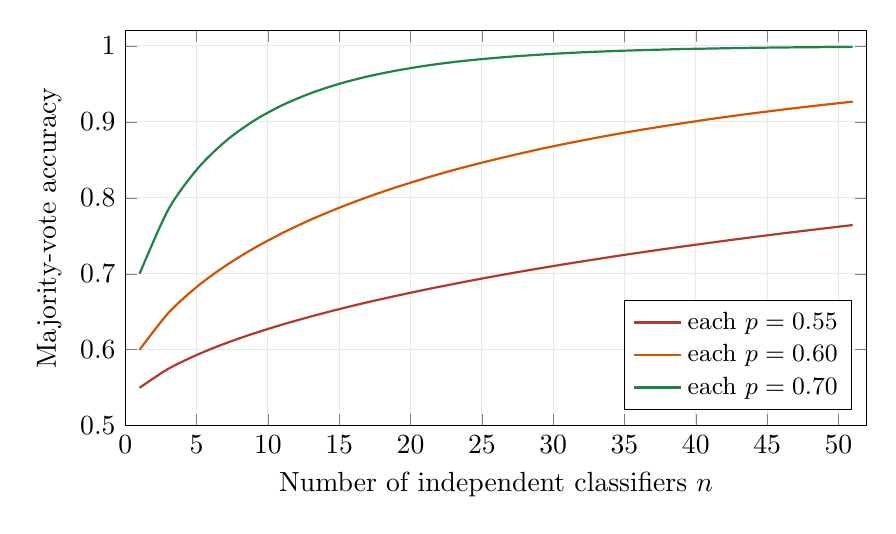
\begin{tikzpicture}
\begin{axis}[width=11cm,height=6.6cm,xlabel={Number of independent classifiers $n$},ylabel={Majority-vote accuracy},
  xmin=0,xmax=52,ymin=0.5,ymax=1.02,grid=both,grid style={gray!18},
  legend style={at={(0.98,0.04)},anchor=south east,font=\small}]
\addplot[thick,mlred,smooth] coordinates {(1,0.55)(3,0.5748)(5,0.5931)(7,0.6083)(9,0.6214)(11,0.6331)(13,0.6437)(15,0.6535)(17,0.6626)(19,0.6710)(21,0.6790)(23,0.6865)(25,0.6937)(27,0.7005)(29,0.7070)(31,0.7132)(33,0.7191)(35,0.7249)(37,0.7304)(39,0.7357)(41,0.7408)(43,0.7458)(45,0.7506)(47,0.7552)(49,0.7597)(51,0.7641)};
\addlegendentry{each $p=0.55$}
\addplot[thick,mlorange,smooth] coordinates {(1,0.6)(3,0.648)(5,0.6826)(7,0.7102)(9,0.7334)(11,0.7535)(13,0.7712)(15,0.7869)(17,0.8011)(19,0.8139)(21,0.8256)(23,0.8364)(25,0.8462)(27,0.8553)(29,0.8638)(31,0.8716)(33,0.8789)(35,0.8857)(37,0.8920)(39,0.8979)(41,0.9035)(43,0.9087)(45,0.9135)(47,0.9181)(49,0.9224)(51,0.9265)};
\addlegendentry{each $p=0.60$}
\addplot[thick,mlgreen,smooth] coordinates {(1,0.7)(3,0.784)(5,0.8369)(7,0.8740)(9,0.9012)(11,0.9218)(13,0.9376)(15,0.9500)(17,0.9597)(19,0.9674)(21,0.9736)(23,0.9786)(25,0.9825)(27,0.9857)(29,0.9883)(31,0.9905)(33,0.9922)(35,0.9936)(37,0.9947)(39,0.9957)(41,0.9964)(43,0.9971)(45,0.9976)(47,0.9980)(49,0.9983)(51,0.9986)};
\addlegendentry{each $p=0.70$}
\end{axis}
\end{tikzpicture}
\caption{Accuracy of a majority vote of $n$ \emph{independent} classifiers, each with accuracy $p$.}\label{fig:majority}
\end{figure}

\begin{explain}
The horizontal axis is the \textbf{number of classifiers} voting and the vertical axis is the \textbf{accuracy of the majority vote}. Each curve is for a different accuracy of the \emph{individual} classifiers (red $55\%$, orange $60\%$, green $70\%$).

\medskip
Look at the \textbf{green curve}: with one classifier the accuracy is $70\%$; with $5$ it is $83.7\%$; with $21$ it is $97.4\%$; with $51$ it is almost $100\%$. Even the \textbf{red curve}, built from classifiers that are barely better than guessing ($55\%$), climbs steadily to about $76\%$ with $51$ voters.

\medskip
\textbf{Important warning:} this picture assumes the classifiers make \emph{independent} errors. In practice they are trained on the same data and their errors are \emph{correlated}, so real gains are smaller. This is why we work hard to make the members \textbf{diverse}.
\end{explain}

\begin{keyidea}
\textbf{Ensembles work best when the members are (i) each better than random guessing and (ii) as different from each other as possible.} Diversity can come from different \emph{algorithms}, different \emph{training samples}, different \emph{features}, or different \emph{hyperparameters}.
\end{keyidea}

\subsection{Types of Ensemble Methods}

\begin{figure}[!htbp]
\centering
\resizebox{\linewidth}{!}{%
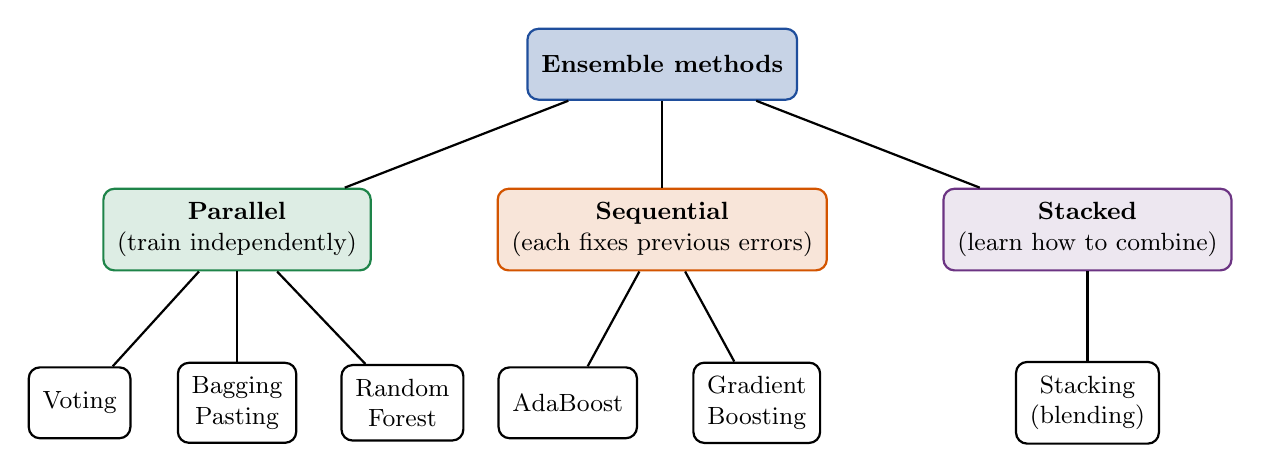
\begin{tikzpicture}[
  n/.style={draw,rounded corners,thick,align=center,font=\small,minimum height=0.9cm,inner sep=5pt},
  arr/.style={thick}]
\node[n,fill=mlblue!25,draw=mlblue] (root) at (0,0) {\textbf{Ensemble methods}};
\node[n,fill=mlgreen!15,draw=mlgreen] (par) at (-5.4,-2.1) {\textbf{Parallel}\\(train independently)};
\node[n,fill=mlorange!15,draw=mlorange] (seq) at (0,-2.1) {\textbf{Sequential}\\(each fixes previous errors)};
\node[n,fill=mlpurple!12,draw=mlpurple] (stk) at (5.4,-2.1) {\textbf{Stacked}\\(learn how to combine)};
\node[n,fill=white] (v) at (-7.4,-4.3) {Voting};
\node[n,fill=white] (b) at (-5.4,-4.3) {Bagging\\Pasting};
\node[n,fill=white] (rf) at (-3.3,-4.3) {Random\\Forest};
\node[n,fill=white] (ad) at (-1.2,-4.3) {AdaBoost};
\node[n,fill=white] (gb) at (1.2,-4.3) {Gradient\\Boosting};
\node[n,fill=white] (st) at (5.4,-4.3) {Stacking\\(blending)};
\foreach \a in {par,seq,stk} \draw[arr] (root)--(\a);
\foreach \a in {v,b,rf} \draw[arr] (par)--(\a);
\foreach \a in {ad,gb} \draw[arr] (seq)--(\a);
\draw[arr] (stk)--(st);
\end{tikzpicture}}
\caption{Families of ensemble methods covered in this chapter.}\label{fig:enstax}
\end{figure}

\begin{explain}
Read the tree from top to bottom. The three coloured boxes are the three \textbf{strategies}.

\begin{itemize}
  \item \textbf{Parallel} (green): the models are trained \emph{independently} (possibly on different samples of the data) and their outputs are combined by voting or averaging. The aim is to reduce \textbf{variance}.
  \item \textbf{Sequential} (orange): models are trained \emph{one after another}, and each new model concentrates on the mistakes of the earlier ones. The aim is to reduce \textbf{bias}.
  \item \textbf{Stacked} (purple): a second-level model \emph{learns} the best way to combine the first-level models.
\end{itemize}
\end{explain}

\begin{theory}{Ensemble Learning}
\tpart{Definition}
\textbf{Ensemble learning} is a machine-learning technique that trains \emph{multiple base models} and \textbf{combines their predictions} (by voting, averaging or a learned combiner) to obtain better accuracy and robustness than any single model.

\tpart{Working}
\begin{enumerate}[itemsep=2pt,topsep=3pt]
  \item Create several base learners, making them \emph{diverse} (different algorithms, data samples or features).
  \item Train each base learner.
  \item Combine the predictions: majority/weighted vote for classification, average for regression, or a meta-model.
  \item Evaluate the ensemble on unseen test data.
\end{enumerate}

\tpart{Assumptions}
\begin{itemize}[itemsep=2pt,topsep=3pt]
  \item Each base learner is better than random guessing
  \item The learners make \emph{different} (ideally independent) errors
\end{itemize}

\tpart{Advantages}
\begin{itemize}[itemsep=2pt,topsep=3pt]
  \item Higher accuracy than a single model
  \item Reduces overfitting (lower variance) and is more robust to noise
  \item Works with almost any base algorithm
\end{itemize}

\tpart{Disadvantages}
\begin{itemize}[itemsep=2pt,topsep=3pt]
  \item More computation, memory and prediction time
  \item Harder to interpret than a single model
  \item Gains are small if the members are too similar
\end{itemize}

\tpart{Applications}
\begin{itemize}[itemsep=2pt,topsep=3pt]
  \item Credit scoring and fraud detection
  \item Medical diagnosis and recommender systems
  \item Winning solutions in data-science competitions
\end{itemize}
\end{theory}

%====================================================================
\section{Voting Classifiers}

\begin{theory}{Voting Classifier}
\tpart{Definition}
A \textbf{voting classifier} combines several \emph{different} classifiers trained on the \emph{same data}. In \textbf{hard voting} the final class is the one predicted by the \emph{majority} of the classifiers; in \textbf{soft voting} the predicted class \emph{probabilities} are averaged and the class with the highest average probability wins.

\tpart{Working}
\begin{enumerate}[itemsep=2pt,topsep=3pt]
  \item Train several diverse classifiers (e.g.\ logistic regression, SVM, random forest) on the same training set.
  \item \textbf{Hard voting:} each classifier predicts a class; count the votes; choose the most frequent class.
  \item \textbf{Soft voting:} each classifier outputs $P(\text{class})$; compute $\bar P(c)=\frac1m\sum_j P_j(c)$ (optionally weighted); choose $\argmax_c\bar P(c)$.
\end{enumerate}

\tpart{Assumptions}
\begin{itemize}[itemsep=2pt,topsep=3pt]
  \item Classifiers are reasonably accurate and diverse
  \item (Soft voting) every classifier can output well-calibrated probabilities
\end{itemize}

\tpart{Advantages}
\begin{itemize}[itemsep=2pt,topsep=3pt]
  \item Very simple to build and often beats the best single member
  \item Soft voting uses the classifiers' \emph{confidence}
\end{itemize}

\tpart{Disadvantages}
\begin{itemize}[itemsep=2pt,topsep=3pt]
  \item Poor members or highly similar members add little
  \item Needs several trained models, hence more cost
\end{itemize}

\tpart{Applications}
\begin{itemize}[itemsep=2pt,topsep=3pt]
  \item Combining different algorithms for text, image or tabular classification
\end{itemize}
\end{theory}

\begin{figure}[!htbp]
\centering
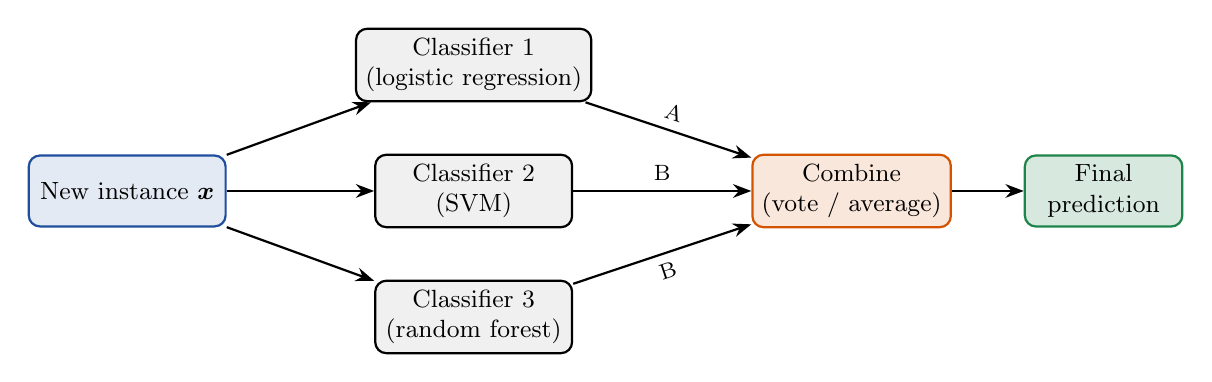
\begin{tikzpicture}[
  b/.style={draw,rounded corners,thick,align=center,font=\small,minimum height=0.9cm,minimum width=2.5cm},
  arr/.style={-{Stealth},thick}]
\node[b,fill=mlblue!12,draw=mlblue] (x) at (0,0) {New instance $\vect x$};
\node[b,fill=gray!12] (c1) at (4.4,1.6) {Classifier 1\\(logistic regression)};
\node[b,fill=gray!12] (c2) at (4.4,0) {Classifier 2\\(SVM)};
\node[b,fill=gray!12] (c3) at (4.4,-1.6) {Classifier 3\\(random forest)};
\node[b,fill=mlorange!14,draw=mlorange,minimum width=2.2cm] (v) at (9.2,0) {Combine\\(vote / average)};
\node[b,fill=mlgreen!18,draw=mlgreen,minimum width=2cm] (y) at (12.4,0) {Final\\prediction};
\foreach \c/\t in {c1/{A},c2/{B},c3/{B}} \draw[arr] (x)--(\c);
\draw[arr] (c1)--(v) node[midway,above,font=\footnotesize,sloped]{A};
\draw[arr] (c2)--(v) node[midway,above,font=\footnotesize]{B};
\draw[arr] (c3)--(v) node[midway,below,font=\footnotesize,sloped]{B};
\draw[arr] (v)--(y);
\end{tikzpicture}
\caption{A voting ensemble: three classifiers vote on the same instance.}\label{fig:voting}
\end{figure}

\begin{explain}
Follow the arrows from left to right. The \textbf{same instance} $\vect x$ is given to three \emph{different} classifiers. Each returns its own answer (labels A, B, B on the arrows). The orange box combines them: in \textbf{hard voting} it counts the votes (two B's against one A), so the \textbf{final prediction is B}. Notice that classifier~1 made a ``mistake'' but the ensemble still reached the answer the majority agreed on.
\end{explain}

\subsection{Hard vs.\ Soft Voting: Worked Example}

\begin{example}[: Which class is the new e-mail?]
Three classifiers estimate the probability that an e-mail is \textbf{spam} (class A); the other class is not-spam (B).

\medskip
\begin{center}
\begin{tabular}{@{}lccc@{}}
\toprule
\textbf{Classifier} & $P(\text{A})$ & $P(\text{B})$ & \textbf{Own prediction}\\
\midrule
1 (logistic regression) & $0.90$ & $0.10$ & A\\
2 (SVM) & $0.40$ & $0.60$ & B\\
3 (random forest) & $0.40$ & $0.60$ & B\\
\bottomrule
\end{tabular}
\end{center}

\medskip
\textbf{Hard voting:} votes are A, B, B $\Rightarrow$ \textbf{B} wins, $2$ to $1$.

\medskip
\textbf{Soft voting:} average probability of A is
\[
  \bar P(A)=\frac{0.90+0.40+0.40}{3}=\frac{1.70}{3}=0.567,\qquad
  \bar P(B)=0.433\ \Rightarrow\ \textbf{A wins}.
\]

\textbf{Why the difference?} Classifier~1 is \emph{very confident} ($90\%$) while the other two are only \emph{mildly} sure ($60\%$). Soft voting lets confident classifiers count for more.

\medskip
\textbf{Weighted soft voting:} if we trust classifier~1 three times as much (weights $3,1,1$):
\[
  \bar P(A)=\frac{3(0.90)+1(0.40)+1(0.40)}{3+1+1}=\frac{3.5}{5}=0.70\ \Rightarrow\ \textbf{A}.
\]
\end{example}

For \textbf{regression}, the ensemble simply \textbf{averages} the predictions: $\hat y=\frac1m\sum_{j=1}^{m}\hat y_j$.

\begin{center}
\begin{tabular}{@{}p{3.1cm}p{5.4cm}p{5.4cm}@{}}
\toprule
 & \textbf{Hard voting} & \textbf{Soft voting}\\
\midrule
Uses & Predicted class labels & Predicted probabilities\\
Rule & Majority vote & Highest average probability\\
Needs probabilities? & No & Yes\\
Accuracy & Good & Usually slightly better\\
\bottomrule
\end{tabular}
\end{center}

%====================================================================
\section{Bagging and Pasting}

Voting uses \emph{different algorithms} on the same data. Another way to create diversity is to use the \textbf{same algorithm} but train each copy on a \textbf{different random subset of the training data}.

\begin{definition}[: Bagging and pasting]
Both methods train $B$ copies of the same base learner, each on a random sample of the training set, and combine them by voting (classification) or averaging (regression).
\begin{itemize}
  \item \textbf{Bagging} (\emph{bootstrap aggregating}): samples are drawn \textbf{with replacement}.
  \item \textbf{Pasting}: samples are drawn \textbf{without replacement}.
\end{itemize}
\end{definition}

\subsection{The Bootstrap}

\begin{definition}[: Bootstrap sample]
A \textbf{bootstrap sample} of a dataset of size $n$ is obtained by drawing $n$ instances \emph{at random with replacement}. Some instances appear several times and some do not appear at all.
\end{definition}

\begin{example}[: Drawing one bootstrap sample]
Original data: instances $\{1,2,3,4,5\}$ ($n=5$). One bootstrap sample might be
\[
  \{2,\ 2,\ 5,\ 1,\ 5\}.
\]
Instance 2 and 5 appear twice, instance 1 once, and instances \textbf{3 and 4 are missing}. These missing instances are the \textbf{out-of-bag (OOB)} instances for this sample; they can be used to test the model trained on the sample.
\end{example}

\paragraph{How many instances are left out?} The probability that a particular instance is \emph{not} chosen in one draw is $1-\frac1n$; over $n$ draws it is $(1-\frac1n)^n\to e^{-1}\approx0.368$ for large $n$. Hence

\begin{itemize}
  \item about \textbf{63.2\%} of the instances appear in each bootstrap sample (at least once);
  \item about \textbf{36.8\%} are \textbf{out-of-bag}.
\end{itemize}

(For $n=100$: $0.99^{100}=0.366$; a simulation with $n=1000$ gave $62.2\%$ unique instances.)

\subsection{Algorithm and Aggregation}

\begin{figure}[!htbp]
\centering
\resizebox{\linewidth}{!}{%
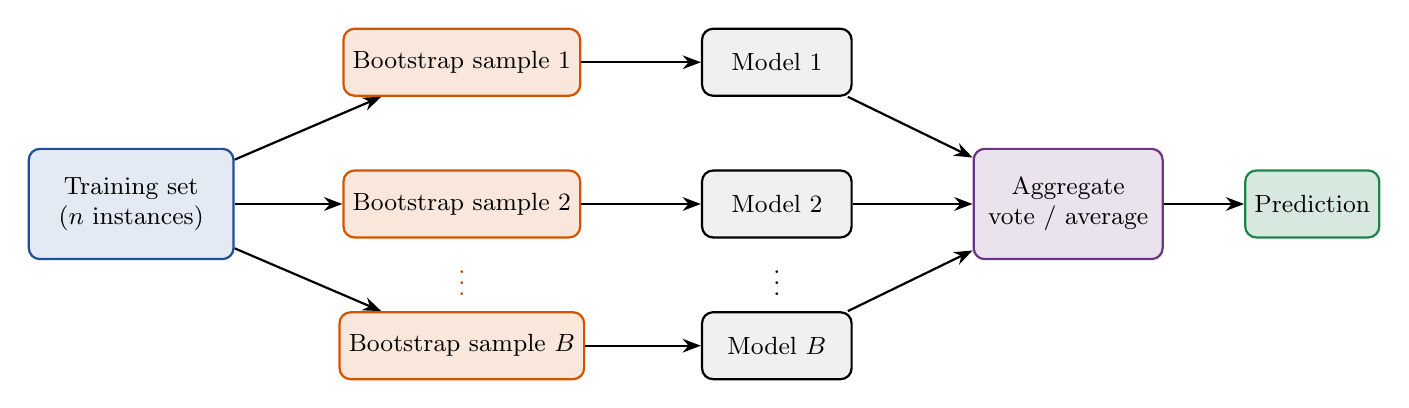
\begin{tikzpicture}[
  b/.style={draw,rounded corners,thick,align=center,font=\small,minimum height=0.85cm},
  arr/.style={-{Stealth},thick}]
\node[b,fill=mlblue!12,draw=mlblue,minimum width=2.6cm,minimum height=1.4cm] (d) at (0,0) {Training set\\$(n$ instances$)$};
\node[b,fill=mlorange!14,draw=mlorange,minimum width=2.8cm] (s1) at (4.2,1.8) {Bootstrap sample 1};
\node[b,fill=mlorange!14,draw=mlorange,minimum width=2.8cm] (s2) at (4.2,0) {Bootstrap sample 2};
\node[b,fill=mlorange!14,draw=mlorange,minimum width=2.8cm] (s3) at (4.2,-1.8) {Bootstrap sample $B$};
\node[b,fill=gray!12,minimum width=1.9cm] (m1) at (8.2,1.8) {Model 1};
\node[b,fill=gray!12,minimum width=1.9cm] (m2) at (8.2,0) {Model 2};
\node[b,fill=gray!12,minimum width=1.9cm] (m3) at (8.2,-1.8) {Model $B$};
\node[b,fill=mlpurple!14,draw=mlpurple,minimum width=2.4cm,minimum height=1.4cm] (a) at (11.9,0) {Aggregate\\vote / average};
\node[b,fill=mlgreen!18,draw=mlgreen] (y) at (15,0) {Prediction};
\foreach \s in {s1,s2,s3} \draw[arr] (d)--(\s);
\foreach \s/\m in {s1/m1,s2/m2,s3/m3} \draw[arr] (\s)--(\m);
\foreach \m in {m1,m2,m3} \draw[arr] (\m)--(a);
\draw[arr] (a)--(y);
\node[font=\small,mlorange!80!black] at (4.2,-0.9) {$\vdots$};
\node[font=\small] at (8.2,-0.9) {$\vdots$};
\end{tikzpicture}}
\caption{The bagging procedure.}\label{fig:bagging}
\end{figure}

\begin{explain}
Start at the blue box on the left. (1)~From the training set we draw $B$ different \textbf{bootstrap samples} (orange). (2)~We train one model on each sample (grey); because the samples differ, the models differ. (3)~For a new instance, every model makes a prediction and the purple box \textbf{aggregates} them: the \textbf{most frequent class} for classification or the \textbf{average} for regression. The models can be trained at the same time (in parallel).
\end{explain}

\paragraph{Why does bagging reduce variance?} Suppose each of $B$ models has prediction variance $\sigma^2$ and any two models have correlation $\rho$. The variance of the average is
\begin{equation}\label{eq:bagvar}
  \Var(\bar f)=\rho\,\sigma^2+\frac{1-\rho}{B}\,\sigma^2 .
\end{equation}

\begin{example}[: Variance of an average of models]
Let $\sigma^2=4$ and $B=10$.
\begin{itemize}
  \item If the models are \textbf{independent} ($\rho=0$): $\Var=\frac{4}{10}=0.4$ (ten times smaller).
  \item If they are \textbf{highly correlated} ($\rho=0.5$): $\Var=0.5(4)+\frac{0.5}{10}(4)=2+0.2=2.2$ (only about half).
  \item Even with $B\to\infty$ the variance cannot go below $\rho\sigma^2=2$.
\end{itemize}
\textbf{Lesson:} averaging helps most when the models are \emph{uncorrelated}; bagging tries to decorrelate them using different bootstrap samples. Bagging reduces \textbf{variance} but \emph{not bias}, so it works best with \textbf{low-bias, high-variance} learners such as deep decision trees.
\end{example}

\subsection{Out-of-Bag (OOB) Evaluation}

Each model never saw about $36.8\%$ of the training instances. We can use these OOB instances as a \emph{free validation set}: for each instance, predict using only the models that did \textbf{not} have it in their sample, and compute the accuracy. The \textbf{OOB score} is a good estimate of test accuracy \emph{without needing a separate validation set}.

\begin{theory}{Bagging and Pasting}
\tpart{Definition}
\textbf{Bagging} (bootstrap aggregating) trains many copies of the same learner, each on a \emph{bootstrap sample} (random sample with replacement) of the training data, and combines their outputs by voting or averaging. \textbf{Pasting} is the same but samples \emph{without replacement}.

\tpart{Working}
\begin{enumerate}[itemsep=2pt,topsep=3pt]
  \item Draw $B$ random samples from the training set (with replacement for bagging).
  \item Train one base learner (e.g.\ a deep decision tree) on each sample.
  \item For a new instance collect the $B$ predictions.
  \item Classification: majority vote; regression: average.
  \item Optionally estimate accuracy using the out-of-bag instances.
\end{enumerate}

\tpart{Assumptions}
\begin{itemize}[itemsep=2pt,topsep=3pt]
  \item The base learner is unstable (small data changes cause large changes in the model)
  \item Bootstrap samples are representative of the population
\end{itemize}

\tpart{Advantages}
\begin{itemize}[itemsep=2pt,topsep=3pt]
  \item Reduces variance and overfitting
  \item Parallel training; free OOB validation
  \item Works with any base learner
\end{itemize}

\tpart{Disadvantages}
\begin{itemize}[itemsep=2pt,topsep=3pt]
  \item Does not reduce bias
  \item Less interpretable and slower than one model
  \item Little gain for stable learners (e.g.\ linear regression)
\end{itemize}

\tpart{Applications}
\begin{itemize}[itemsep=2pt,topsep=3pt]
  \item Improving decision trees (Random Forests)
  \item Noisy data problems, regression and classification
\end{itemize}
\end{theory}

\begin{center}
\begin{tabular}{@{}p{3.2cm}p{5.4cm}p{5.4cm}@{}}
\toprule
 & \textbf{Bagging} & \textbf{Pasting}\\
\midrule
Sampling & With replacement (bootstrap) & Without replacement\\
Duplicates in a sample? & Yes & No\\
OOB evaluation? & Yes (about $37\%$ per model) & Not directly\\
Diversity & Slightly higher & Slightly lower\\
Typical bias / variance & Slightly higher bias, lower variance & Slightly lower bias\\
\bottomrule
\end{tabular}
\end{center}

%====================================================================
\section{Random Forests}

A \textbf{Random Forest} is the most popular ensemble method. It is \textbf{bagging of decision trees} with one extra trick that makes the trees even more different.

\begin{definition}[: Random Forest]
A \textbf{Random Forest} is an ensemble of many decision trees, each trained on a \emph{bootstrap sample} of the data, where at \emph{every split} the tree considers only a \textbf{random subset of the features} (typically $\sqrt p$ for classification and $p/3$ for regression, with $p$ the total number of features). The forest predicts by \emph{majority vote} (classification) or \emph{average} (regression).
\end{definition}

\paragraph{Why the random feature subset?} If one feature is very strong, \emph{every} bagged tree would split on it first and all trees would look alike (high correlation $\rho$ in Equation~\eqref{eq:bagvar}). Forcing each split to choose from a random subset \textbf{decorrelates} the trees, so averaging them reduces the variance much more.

\begin{figure}[!htbp]
\centering
\resizebox{\linewidth}{!}{%
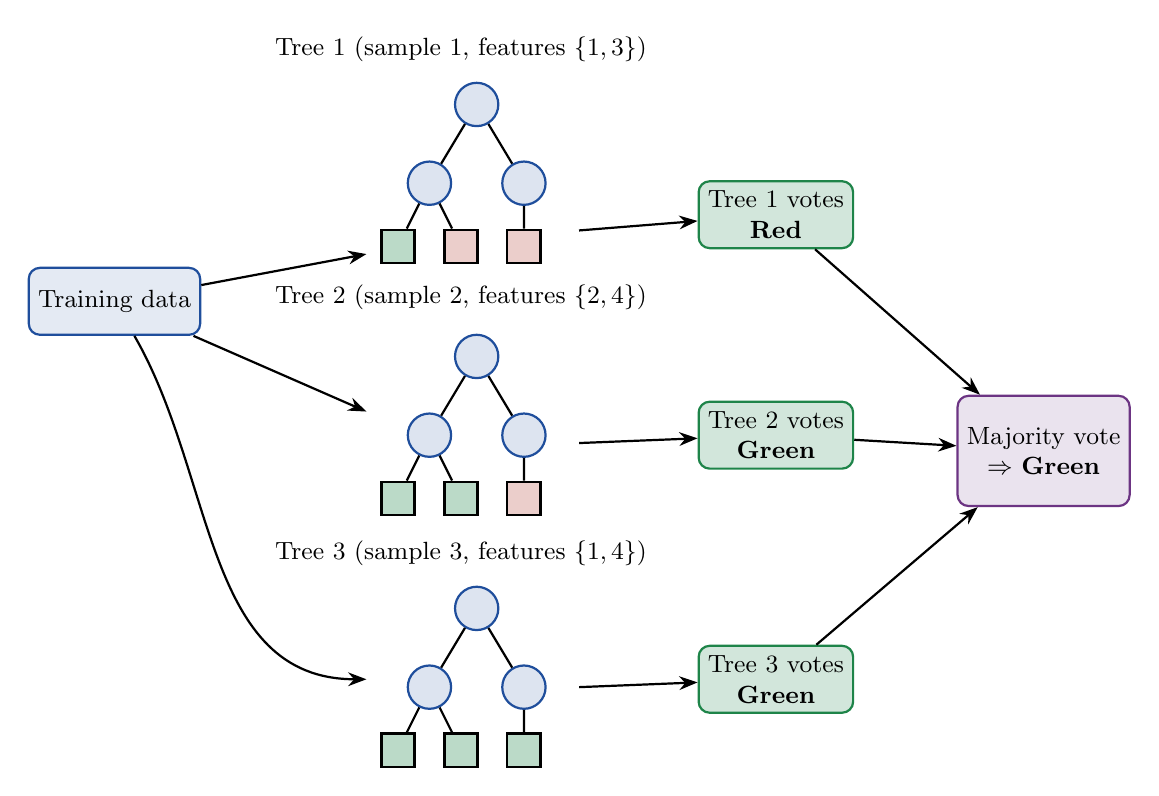
\begin{tikzpicture}[
  b/.style={draw,rounded corners,thick,align=center,font=\small,minimum height=0.85cm},
  arr/.style={-{Stealth},thick},
  nd/.style={circle,draw,thick,fill=mlblue!15,draw=mlblue,minimum size=0.55cm,inner sep=0pt},
  lf/.style={rectangle,draw,thick,minimum size=0.42cm,inner sep=0pt}]
\node[b,fill=mlblue!12,draw=mlblue] (d) at (0,0) {Training data};
% tree 1
\node[nd] (a1) at (4.6,2.5) {}; \node[nd] (a2) at (4.0,1.5) {}; \node[nd] (a3) at (5.2,1.5) {};
\node[lf,fill=mlgreen!30] (a4) at (3.6,0.7) {}; \node[lf,fill=mlred!25] (a5) at (4.4,0.7) {};
\node[lf,fill=mlred!25] (a6) at (5.2,0.7) {};
\draw[thick] (a1)--(a2)--(a4); \draw[thick] (a2)--(a5); \draw[thick] (a1)--(a3)--(a6);
\node[font=\small] at (4.4,3.2) {Tree 1 (sample 1, features $\{1,3\}$)};
% tree 2
\node[nd] (b1) at (4.6,-0.7) {}; \node[nd] (b2) at (4.0,-1.7) {}; \node[nd] (b3) at (5.2,-1.7) {};
\node[lf,fill=mlgreen!30] (b4) at (3.6,-2.5) {}; \node[lf,fill=mlgreen!30] (b5) at (4.4,-2.5) {};
\node[lf,fill=mlred!25] (b6) at (5.2,-2.5) {};
\draw[thick] (b1)--(b2)--(b4); \draw[thick] (b2)--(b5); \draw[thick] (b1)--(b3)--(b6);
\node[font=\small] at (4.4,0.05) {Tree 2 (sample 2, features $\{2,4\}$)};
% tree 3
\node[nd] (c1) at (4.6,-3.9) {}; \node[nd] (c2) at (4.0,-4.9) {}; \node[nd] (c3) at (5.2,-4.9) {};
\node[lf,fill=mlgreen!30] (c4) at (3.6,-5.7) {}; \node[lf,fill=mlgreen!30] (c5) at (4.4,-5.7) {};
\node[lf,fill=mlgreen!30] (c6) at (5.2,-5.7) {};
\draw[thick] (c1)--(c2)--(c4); \draw[thick] (c2)--(c5); \draw[thick] (c1)--(c3)--(c6);
\node[font=\small] at (4.4,-3.2) {Tree 3 (sample 3, features $\{1,4\}$)};
\node[b,fill=mlgreen!20,draw=mlgreen] (p1) at (8.4,1.1) {Tree 1 votes\\\textbf{Red}};
\node[b,fill=mlgreen!20,draw=mlgreen] (p2) at (8.4,-1.7) {Tree 2 votes\\\textbf{Green}};
\node[b,fill=mlgreen!20,draw=mlgreen] (p3) at (8.4,-4.8) {Tree 3 votes\\\textbf{Green}};
\node[b,fill=mlpurple!14,draw=mlpurple,minimum height=1.4cm] (m) at (11.8,-1.9) {Majority vote\\$\Rightarrow$ \textbf{Green}};
\draw[arr] (d)--(3.2,0.6); \draw[arr] (d)--(3.2,-1.4); \draw[arr] (d) to[out=-60,in=180] (3.2,-4.8);
\draw[arr] (5.9,0.9)--(p1); \draw[arr] (5.9,-1.8)--(p2); \draw[arr] (5.9,-4.9)--(p3);
\draw[arr] (p1)--(m); \draw[arr] (p2)--(m); \draw[arr] (p3)--(m);
\end{tikzpicture}}
\caption{A Random Forest of three trees. Each tree sees a different bootstrap sample and different candidate features.}\label{fig:rf}
\end{figure}

\begin{explain}
The training data (left) is turned into \textbf{three different trees}. Each tree is trained on its \emph{own bootstrap sample} and, at each split, can only choose from \emph{its own random features} (shown in brackets), so the trees have different shapes and make different mistakes. The small squares at the bottom of each tree are \textbf{leaves}: red or green squares show the class that leaf predicts. For a new instance each tree sends it down to a leaf and \textbf{votes} for that leaf's class: Tree~1 says Red; Trees~2 and~3 say Green. The forest takes the \textbf{majority}: \textbf{Green}.
\end{explain}

\begin{example}[: Voting in a forest of five trees]
A forest has $5$ trees. For a new patient the trees predict: Disease, Healthy, Disease, Disease, Healthy.

\medskip
\begin{center}
\begin{tabular}{@{}lcc@{}}
\toprule
 & \textbf{Disease} & \textbf{Healthy}\\
\midrule
Votes & 3 & 2\\
Estimated probability & $3/5=0.60$ & $2/5=0.40$\\
\bottomrule
\end{tabular}
\end{center}
\medskip
The forest predicts \textbf{Disease} (with a ``confidence'' of $60\%$). For regression the five tree outputs would be averaged.
\end{example}

\subsection{Feature Importance}

A great by-product: a forest tells us \textbf{which features matter}. A feature's \textbf{importance} is the average total decrease in impurity (Gini or entropy) from all splits that use it, averaged over all trees and normalised so the importances sum to $1$.

\begin{figure}[!htbp]
\centering
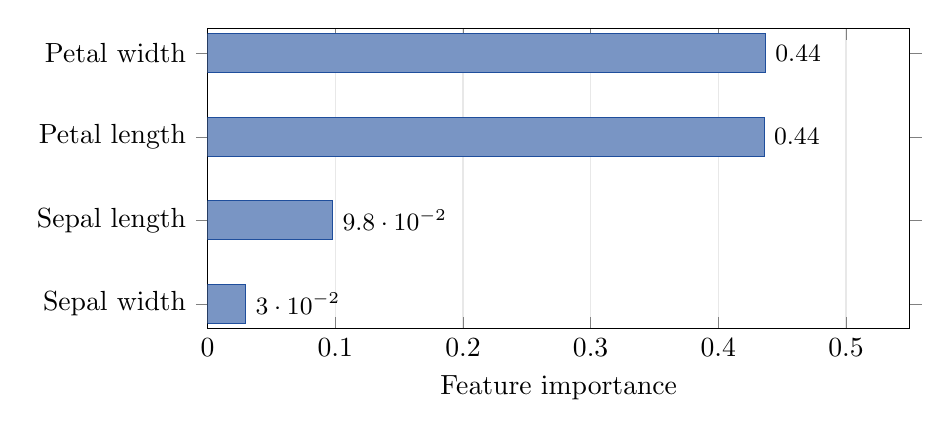
\begin{tikzpicture}
\begin{axis}[xbar,width=10.5cm,height=5.4cm,xlabel={Feature importance},
  symbolic y coords={Sepal width,Sepal length,Petal length,Petal width},ytick=data,
  xmin=0,xmax=0.55,bar width=14pt,nodes near coords,nodes near coords align={horizontal},
  every node near coord/.append style={font=\small},xmajorgrids,grid style={gray!18}]
\addplot[fill=mlblue!60,draw=mlblue] coordinates {(0.030,Sepal width)(0.098,Sepal length)(0.436,Petal length)(0.437,Petal width)};
\end{axis}
\end{tikzpicture}
\caption{Feature importances of a Random Forest (200 trees) on the Iris dataset.}\label{fig:imp}
\end{figure}

\begin{explain}
Each bar is one of the four measurements of an iris flower; a \textbf{longer bar means the forest relied on that feature more}. The two \textbf{petal} measurements together account for about $87\%$ of the importance ($0.436+0.437$), while the \emph{sepal width} contributes only $3\%$. This agrees with the single tree of Chapter~3, which separated all three species using only the petal width. Such a ranking helps in \textbf{feature selection} and in explaining the model to non-experts.
\end{explain}

\begin{theory}{Random Forest}
\tpart{Definition}
A \textbf{Random Forest} is an ensemble of decision trees built by \emph{bagging}, in which each split considers only a \emph{random subset of features}; the final output is the majority vote (classification) or the mean (regression) of the trees.

\tpart{Working}
\begin{enumerate}[itemsep=2pt,topsep=3pt]
  \item Draw $B$ bootstrap samples from the training data.
  \item For each sample grow a decision tree; at \emph{each node} choose the best split from a random subset of $m\approx\sqrt p$ features.
  \item Grow the trees deep (little or no pruning).
  \item Predict by majority vote or average of all trees.
  \item Compute the OOB score and the feature importances.
\end{enumerate}

\tpart{Assumptions}
\begin{itemize}[itemsep=2pt,topsep=3pt]
  \item Individual trees are low-bias but high-variance
  \item Trees are weakly correlated because of the randomisation
\end{itemize}

\tpart{Advantages}
\begin{itemize}[itemsep=2pt,topsep=3pt]
  \item High accuracy; handles many features and mixed data types
  \item Much less overfitting than a single tree
  \item Gives feature importance and OOB error; needs little tuning
\end{itemize}

\tpart{Disadvantages}
\begin{itemize}[itemsep=2pt,topsep=3pt]
  \item Less interpretable than one tree; larger memory
  \item Slower prediction with many trees
  \item May be biased towards features with many categories
\end{itemize}

\tpart{Applications}
\begin{itemize}[itemsep=2pt,topsep=3pt]
  \item Credit-risk and churn prediction
  \item Medical diagnosis, bioinformatics, remote sensing
  \item Feature selection
\end{itemize}
\end{theory}

\paragraph{Main hyperparameters.}
\begin{itemize}
  \item \texttt{n\_estimators}: number of trees (more is better but slower; $100$--$500$ is typical).
  \item \texttt{max\_features}: features tried at each split (default $\sqrt p$).
  \item \texttt{max\_depth}, \texttt{min\_samples\_leaf}: limit the size of each tree.
\end{itemize}

\paragraph{Extra-Trees.} \emph{Extremely Randomised Trees} go one step further and also choose the \emph{split thresholds} at random: faster to train and even lower variance, at the price of a little more bias.

%====================================================================
\section{Boosting}

Bagging trains models \emph{in parallel} to reduce variance. \textbf{Boosting} trains them \textbf{one after another}, each model trying to correct the mistakes of the previous ones. It reduces \textbf{bias}.

\begin{definition}[: Boosting]
\textbf{Boosting} is a sequential ensemble method that combines many \emph{weak learners} into a strong learner by training them in sequence, where each new learner focuses on the instances that the earlier learners handled badly, and the final prediction is a \emph{weighted} combination of all learners.
\end{definition}

\begin{keyidea}
\textbf{Analogy.} A student takes a test, then studies \emph{only the questions answered wrongly}, then takes another test, and so on. After several rounds the student has covered the hard questions that a single reading would have missed.
\end{keyidea}

\subsection{AdaBoost (Adaptive Boosting)}

\textbf{AdaBoost} keeps a \textbf{weight} on every training instance. After each round it \textbf{increases the weights of misclassified instances} so the next learner pays more attention to them. Labels are coded $y_i\in\{-1,+1\}$.

\begin{definition}[: AdaBoost algorithm]
\begin{enumerate}
  \item Initialise weights $w_i=\dfrac1n$ for all $n$ instances.
  \item For $t=1,\dots,T$:
  \begin{enumerate}[label=(\alph*)]
    \item Train a weak learner $h_t$ on the \emph{weighted} data.
    \item Weighted error: $\varepsilon_t=\sum_{i:\,h_t(\vect x_i)\neq y_i}w_i$.
    \item Learner weight (``say''): $\alpha_t=\dfrac12\ln\dfrac{1-\varepsilon_t}{\varepsilon_t}$.
    \item Update weights: $w_i\leftarrow w_i\,e^{-\alpha_t\,y_i\,h_t(\vect x_i)}$, then divide by the sum so that $\sum w_i=1$.\\
    (Correct instances are multiplied by $e^{-\alpha_t}<1$, wrong ones by $e^{+\alpha_t}>1$.)
  \end{enumerate}
  \item Final classifier: $H(\vect x)=\operatorname{sign}\Big(\sum_{t=1}^{T}\alpha_t\,h_t(\vect x)\Big)$.
\end{enumerate}
\end{definition}

\paragraph{Meaning of $\alpha_t$.} A learner with small error gets a \textbf{large} weight, one with error $0.5$ (random guessing) gets $\alpha=0$, and one with error above $0.5$ would get a negative weight.

\medskip
\begin{center}
\begin{tabular}{@{}c|ccccc@{}}
\toprule
Error $\varepsilon_t$ & $0.05$ & $0.10$ & $0.20$ & $0.30$ & $0.50$\\
\midrule
$\alpha_t=\frac12\ln\frac{1-\varepsilon_t}{\varepsilon_t}$ & $1.47$ & $1.10$ & $0.69$ & $0.42$ & $0$\\
\bottomrule
\end{tabular}
\end{center}

\subsubsection*{End-to-end example: five instances, three rounds}

True labels $y=(+1,+1,-1,-1,+1)$ for instances $1,\dots,5$. We use weak learners that are each wrong on only one instance.

\begin{example}[: AdaBoost by hand]
\textbf{Round 1.} Weights $w=(0.2,0.2,0.2,0.2,0.2)$.

Weak learner $h_1$ predicts $(+,+,-,+,+)$: it is wrong only on \textbf{instance 4}.
\[
  \varepsilon_1=0.2,\qquad \alpha_1=\tfrac12\ln\tfrac{0.8}{0.2}=\tfrac12\ln4=0.693 .
\]
Update: correct instances $\times e^{-0.693}=\times0.5$; instance 4 $\times e^{0.693}=\times2$.
\[
  (0.1,\,0.1,\,0.1,\,0.4,\,0.1)\ \xrightarrow{\ \text{sum}=0.8\ }\ w=(0.125,\,0.125,\,0.125,\,\mathbf{0.5},\,0.125).
\]

\medskip
\textbf{Round 2.} Instance 4 now carries half of the total weight, so $h_2$ must get it right. Say $h_2$ predicts $(-,+,-,-,+)$: wrong only on \textbf{instance 1}.
\[
  \varepsilon_2=0.125,\qquad \alpha_2=\tfrac12\ln\tfrac{0.875}{0.125}=\tfrac12\ln7=0.973 .
\]
Correct $\times e^{-0.973}=0.378$; instance 1 $\times e^{0.973}=2.646$. After normalising:
\[
  w=(\mathbf{0.500},\,0.071,\,0.071,\,0.286,\,0.071).
\]

\medskip
\textbf{Round 3.} Now instance 1 dominates. Say $h_3$ predicts $(+,+,+,-,+)$: wrong only on \textbf{instance 3}.
\[
  \varepsilon_3=0.071,\qquad \alpha_3=\tfrac12\ln\tfrac{0.929}{0.071}=\tfrac12\ln13=1.282 .
\]

\medskip
\textbf{Final ensemble:} $H(\vect x)=\operatorname{sign}\big(0.693\,h_1+0.973\,h_2+1.282\,h_3\big)$.

\begin{center}
\begin{tabular}{@{}c|cccccc|c@{}}
\toprule
Instance & $y$ & $h_1$ & $h_2$ & $h_3$ & Score & $H$ & Correct?\\
\midrule
1 & $+$ & $+$ & $-$ & $+$ & $0.693-0.973+1.282=+1.00$ & $+$ & \checkmark\\
2 & $+$ & $+$ & $+$ & $+$ & $+2.95$ & $+$ & \checkmark\\
3 & $-$ & $-$ & $-$ & $+$ & $-0.693-0.973+1.282=-0.38$ & $-$ & \checkmark\\
4 & $-$ & $+$ & $-$ & $-$ & $0.693-0.973-1.282=-1.56$ & $-$ & \checkmark\\
5 & $+$ & $+$ & $+$ & $+$ & $+2.95$ & $+$ & \checkmark\\
\bottomrule
\end{tabular}
\end{center}

\textbf{Conclusion:} each weak learner made a mistake, but the weighted ensemble classifies \emph{all five} instances correctly.
\end{example}

\begin{figure}[!htbp]
\centering
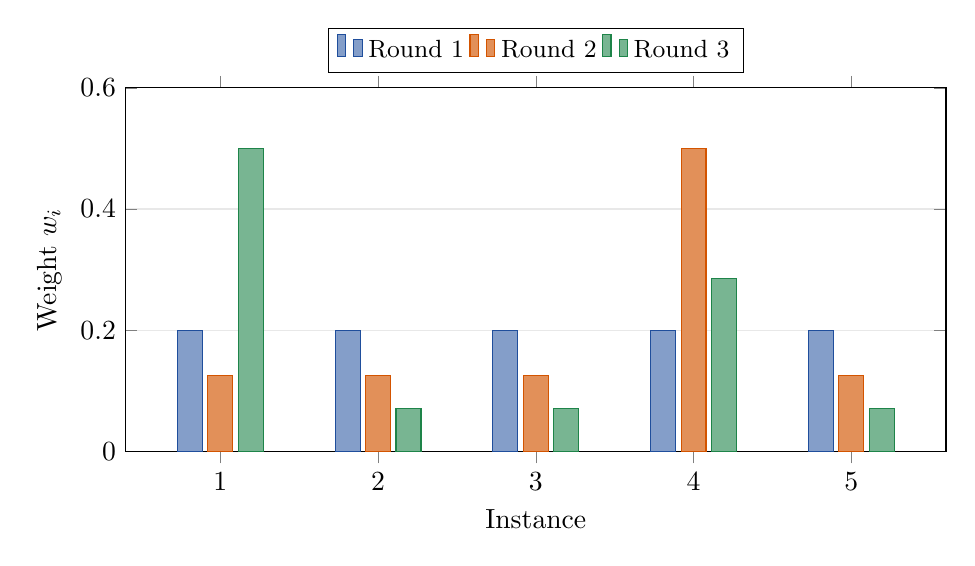
\begin{tikzpicture}
\begin{axis}[ybar,width=12cm,height=6.2cm,bar width=9pt,xlabel={Instance},ylabel={Weight $w_i$},
  symbolic x coords={1,2,3,4,5},xtick=data,ymin=0,ymax=0.6,enlarge x limits=0.15,
  legend style={at={(0.5,1.04)},anchor=south,legend columns=3,font=\small},ymajorgrids,grid style={gray!18}]
\addplot[fill=mlblue!55,draw=mlblue] coordinates {(1,0.2)(2,0.2)(3,0.2)(4,0.2)(5,0.2)};
\addplot[fill=mlorange!65,draw=mlorange] coordinates {(1,0.125)(2,0.125)(3,0.125)(4,0.5)(5,0.125)};
\addplot[fill=mlgreen!60,draw=mlgreen] coordinates {(1,0.5)(2,0.071)(3,0.071)(4,0.286)(5,0.071)};
\legend{Round 1,Round 2,Round 3}
\end{axis}
\end{tikzpicture}
\caption{How AdaBoost's instance weights change from round to round in the worked example.}\label{fig:adaw}
\end{figure}

\begin{explain}
Each group of bars is one training instance; the three bars show its weight at the start of Round~1 (blue), Round~2 (orange) and Round~3 (green).

\begin{itemize}
  \item \textbf{Round 1 (blue):} all instances are equal ($0.2$).
  \item \textbf{Round 2 (orange):} instance~4, which learner~1 got wrong, has jumped to $0.5$.
  \item \textbf{Round 3 (green):} instance~1, which learner~2 got wrong, now has the biggest weight ($0.5$) while instance~4 (now handled) has dropped back to $0.286$.
\end{itemize}
The \textbf{spotlight moves} to whichever instances are still being misclassified. This is how boosting makes later learners specialise in the hard cases.
\end{explain}

\begin{theory}{AdaBoost}
\tpart{Definition}
\textbf{AdaBoost} (Adaptive Boosting) is a \emph{sequential} ensemble algorithm that builds a strong classifier as a \emph{weighted vote of weak learners} (usually decision stumps), re-weighting the training instances after every round so that misclassified instances get more attention.

\tpart{Working}
\begin{enumerate}[itemsep=2pt,topsep=3pt]
  \item Start with equal instance weights $w_i=1/n$.
  \item Train a weak learner on the weighted data and compute its weighted error $\varepsilon_t$.
  \item Compute its weight $\alpha_t=\frac12\ln\frac{1-\varepsilon_t}{\varepsilon_t}$.
  \item Increase the weights of misclassified instances, decrease the others, and normalise.
  \item Repeat for $T$ rounds; predict $H(\vect x)=\operatorname{sign}\sum_t\alpha_th_t(\vect x)$.
\end{enumerate}

\tpart{Assumptions}
\begin{itemize}[itemsep=2pt,topsep=3pt]
  \item Each weak learner is slightly better than random guessing ($\varepsilon_t<0.5$)
  \item Data are not dominated by label noise
\end{itemize}

\tpart{Advantages}
\begin{itemize}[itemsep=2pt,topsep=3pt]
  \item Turns weak learners into a strong one; reduces bias
  \item Few hyperparameters; simple to implement
\end{itemize}

\tpart{Disadvantages}
\begin{itemize}[itemsep=2pt,topsep=3pt]
  \item Sensitive to noisy data and outliers (they keep gaining weight)
  \item Sequential, so it cannot be parallelised
\end{itemize}

\tpart{Applications}
\begin{itemize}[itemsep=2pt,topsep=3pt]
  \item Face detection (Viola--Jones)
  \item Text and customer classification
\end{itemize}
\end{theory}

\subsection{Gradient Boosting}

\textbf{Gradient boosting} generalises the idea. Instead of re-weighting instances it fits each new model to the \textbf{residuals} (errors) of the current ensemble.

\begin{definition}[: Gradient boosting (regression with squared loss)]
\begin{enumerate}
  \item Start with a constant prediction $F_0(\vect x)=\bar y$ (the mean).
  \item For $m=1,\dots,M$:
  \begin{enumerate}[label=(\alph*)]
    \item Compute the \textbf{residuals} $r_i=y_i-F_{m-1}(\vect x_i)$ (they are the negative gradient of the squared-error loss).
    \item Fit a small tree $h_m$ to predict the residuals.
    \item Update: $F_m(\vect x)=F_{m-1}(\vect x)+\eta\,h_m(\vect x)$, where $\eta\in(0,1]$ is the \textbf{learning rate} (shrinkage).
  \end{enumerate}
  \item The final model is $F_M(\vect x)=\bar y+\eta\sum_{m=1}^{M}h_m(\vect x)$.
\end{enumerate}
\end{definition}

\begin{example}[: Gradient boosting on four points]
Predict a salary (in thousand rupees) from years of experience $x$:

\medskip
\begin{center}
\begin{tabular}{@{}c|cccc@{}}
\toprule
$x$ & 1 & 2 & 3 & 4\\
$y$ & 10 & 12 & 20 & 22\\
\bottomrule
\end{tabular}
\end{center}

\medskip
Use a decision stump that splits at $x\le2.5$ and $\eta=0.5$.

\medskip
\textbf{Step 0.} $F_0=\bar y=\frac{10+12+20+22}{4}=16$ for all $x$. Residuals $r=(-6,-4,4,6)$; $\text{MSE}=\frac{36+16+16+36}{4}=\mathbf{26}$.

\medskip
\textbf{Step 1.} The stump predicts the mean residual on each side: left $\frac{-6-4}{2}=-5$, right $\frac{4+6}{2}=5$.
\[
  F_1=F_0+0.5\,h_1=(16-2.5,\ 16-2.5,\ 16+2.5,\ 16+2.5)=(13.5,\ 13.5,\ 18.5,\ 18.5).
\]
New residuals $(10-13.5,\ 12-13.5,\ 20-18.5,\ 22-18.5)=(-3.5,-1.5,1.5,3.5)$; $\text{MSE}=\frac{12.25+2.25+2.25+12.25}{4}=\mathbf{7.25}$.

\medskip
\textbf{Step 2.} Stump on the new residuals: left $-2.5$, right $+2.5$.
\[
  F_2=F_1+0.5\,h_2=(12.25,\ 12.25,\ 19.75,\ 19.75).
\]
Residuals $(-2.25,-0.25,0.25,2.25)$; $\text{MSE}=\frac{5.06+0.06+0.06+5.06}{4}=\mathbf{2.56}$.

\medskip
\begin{center}
\begin{tabular}{@{}lccc@{}}
\toprule
\textbf{Stage} & $F_0$ & $F_1$ & $F_2$\\
\midrule
MSE & 26.0 & 7.25 & 2.56\\
\bottomrule
\end{tabular}
\end{center}
The error falls at every stage. Prediction for $x=3$: $F_2(3)=19.75$ (true value 20).
\end{example}

\begin{figure}[!htbp]
\centering
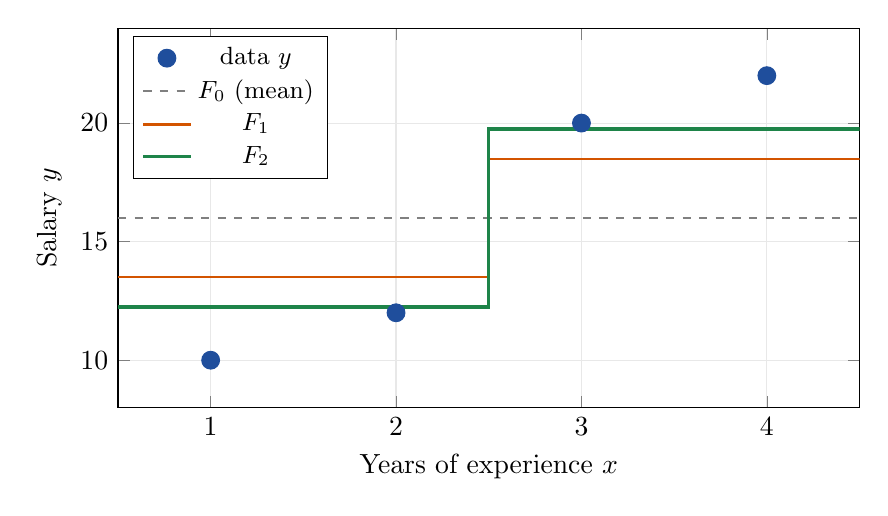
\begin{tikzpicture}
\begin{axis}[width=11cm,height=6.4cm,xlabel={Years of experience $x$},ylabel={Salary $y$},
  xmin=0.5,xmax=4.5,ymin=8,ymax=24,grid=both,grid style={gray!18},xtick={1,2,3,4},
  legend style={at={(0.02,0.98)},anchor=north west,font=\small}]
\addplot[only marks,mark=*,mlblue,mark size=3.2pt] coordinates {(1,10)(2,12)(3,20)(4,22)};
\addlegendentry{data $y$}
\addplot[thick,gray,dashed] coordinates {(0.5,16)(4.5,16)};
\addlegendentry{$F_0$ (mean)}
\addplot[thick,mlorange] coordinates {(0.5,13.5)(2.5,13.5)(2.5,18.5)(4.5,18.5)};
\addlegendentry{$F_1$}
\addplot[very thick,mlgreen] coordinates {(0.5,12.25)(2.5,12.25)(2.5,19.75)(4.5,19.75)};
\addlegendentry{$F_2$}
\end{axis}
\end{tikzpicture}
\caption{Gradient boosting: each stage moves the step-function prediction closer to the data.}\label{fig:gbfit}
\end{figure}

\begin{explain}
The blue dots are the data. The \textbf{grey dashed line} is the starting guess $F_0$: the mean, a flat line that is wrong for every point. The \textbf{orange step function} $F_1$ moves the left points down and the right points up, getting closer. The \textbf{green step function} $F_2$ is closer still: its left step ($12.25$) is near the left points ($10,12$) and its right step ($19.75$) is near ($20,22$). Each stage \emph{adds a small correction} to fix the remaining error. With many stages and deeper trees, the curve can follow complex patterns.
\end{explain}

\paragraph{Learning rate and number of stages.} A small $\eta$ (e.g.\ $0.1$) makes learning slower but usually generalises better; it must be balanced with the number of trees $M$ (small $\eta$ needs large $M$). Too many stages can \textbf{overfit}; use early stopping on a validation set. Popular fast implementations are \textbf{XGBoost}, \textbf{LightGBM} and \textbf{CatBoost}.

\begin{theory}{Gradient Boosting}
\tpart{Definition}
\textbf{Gradient boosting} builds an additive model $F_M(\vect x)=F_0+\eta\sum_mh_m(\vect x)$ \emph{stage by stage}, where each new weak learner $h_m$ is fitted to the \textbf{negative gradient of the loss} (the \emph{residuals}, for squared error) of the current model.

\tpart{Working}
\begin{enumerate}[itemsep=2pt,topsep=3pt]
  \item Initialise with a constant prediction (e.g.\ the mean).
  \item Compute the residuals of the current model.
  \item Fit a small decision tree to the residuals.
  \item Add the tree to the model scaled by the learning rate $\eta$.
  \item Repeat for $M$ stages (stop early on a validation set).
\end{enumerate}

\tpart{Assumptions}
\begin{itemize}[itemsep=2pt,topsep=3pt]
  \item A differentiable loss function suited to the task
  \item Weak learners are simple (shallow trees)
\end{itemize}

\tpart{Advantages}
\begin{itemize}[itemsep=2pt,topsep=3pt]
  \item Very high accuracy on structured/tabular data
  \item Works for regression, classification and ranking with any differentiable loss
\end{itemize}

\tpart{Disadvantages}
\begin{itemize}[itemsep=2pt,topsep=3pt]
  \item Many hyperparameters to tune (learning rate, depth, number of trees)
  \item Can overfit noisy data; sequential training is slower
\end{itemize}

\tpart{Applications}
\begin{itemize}[itemsep=2pt,topsep=3pt]
  \item Web search ranking, click-through-rate prediction
  \item Credit scoring and sales forecasting
\end{itemize}
\end{theory}

\begin{center}
\small
\begin{tabular}{@{}p{3.1cm}p{5.5cm}p{5.5cm}@{}}
\toprule
 & \textbf{AdaBoost} & \textbf{Gradient boosting}\\
\midrule
How errors are handled & Re-weights misclassified instances & Fits new learner to the residuals\\
Loss function & Exponential loss & Any differentiable loss\\
Combination & Weighted vote $\sum\alpha_th_t$ & Sum $F_0+\eta\sum h_m$\\
Weak learner & Usually a stump & Small tree (depth 3--8)\\
\bottomrule
\end{tabular}
\end{center}

%====================================================================
\section{Stacking}

Voting uses a fixed rule (majority, average). \textbf{Stacking} (stacked generalisation) asks: \emph{why not train a model to learn the best way to combine the predictions?}

\begin{definition}[: Stacking]
\textbf{Stacking} trains several different \textbf{base learners} (level-0) and then trains a \textbf{meta-learner} (level-1, also called the \emph{blender}) whose \emph{inputs are the predictions of the base learners} and whose output is the final prediction.
\end{definition}

\begin{figure}[!htbp]
\centering
\resizebox{\linewidth}{!}{%
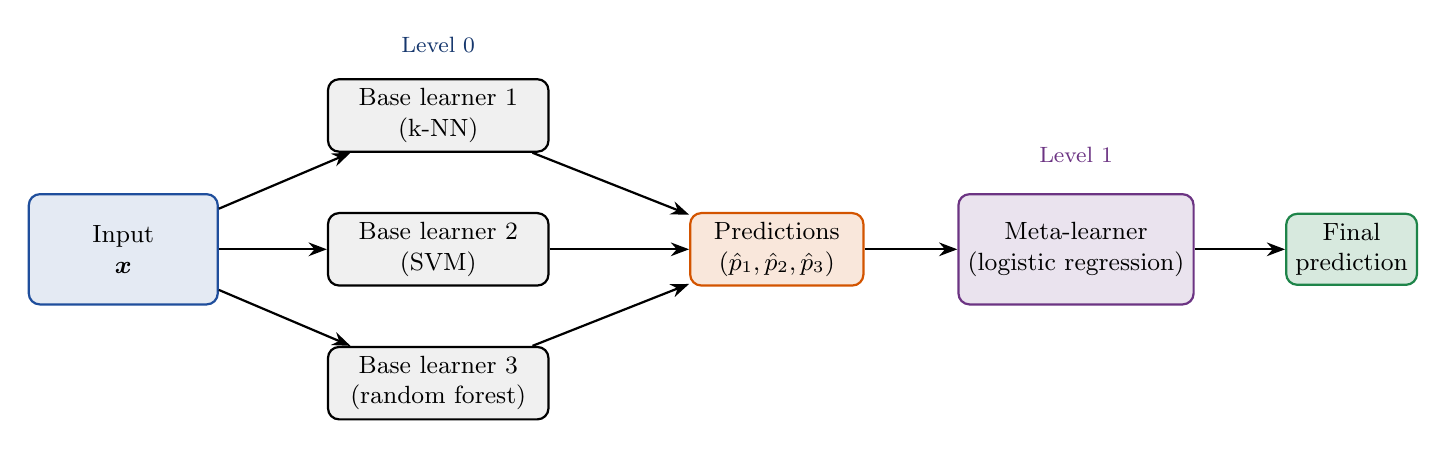
\begin{tikzpicture}[
  b/.style={draw,rounded corners,thick,align=center,font=\small,minimum height=0.9cm},
  arr/.style={-{Stealth},thick}]
\node[b,fill=mlblue!12,draw=mlblue,minimum width=2.4cm,minimum height=1.4cm] (x) at (0,0) {Input\\$\vect x$};
\node[b,fill=gray!12,minimum width=2.8cm] (b1) at (4,1.7) {Base learner 1\\(k-NN)};
\node[b,fill=gray!12,minimum width=2.8cm] (b2) at (4,0) {Base learner 2\\(SVM)};
\node[b,fill=gray!12,minimum width=2.8cm] (b3) at (4,-1.7) {Base learner 3\\(random forest)};
\node[b,fill=mlorange!14,draw=mlorange,minimum width=2.2cm] (f) at (8.3,0) {Predictions\\$(\hat p_1,\hat p_2,\hat p_3)$};
\node[b,fill=mlpurple!14,draw=mlpurple,minimum width=2.8cm,minimum height=1.4cm] (m) at (12.1,0) {Meta-learner\\(logistic regression)};
\node[b,fill=mlgreen!18,draw=mlgreen] (y) at (15.6,0) {Final\\prediction};
\foreach \b in {b1,b2,b3} {\draw[arr] (x)--(\b); \draw[arr] (\b)--(f);}
\draw[arr] (f)--(m); \draw[arr] (m)--(y);
\node[font=\footnotesize,mlblue!70!black] at (4,2.6) {Level 0};
\node[font=\footnotesize,mlpurple] at (12.1,1.2) {Level 1};
\end{tikzpicture}}
\caption{Architecture of a stacking ensemble.}\label{fig:stack}
\end{figure}

\begin{explain}
The input goes to three \textbf{level-0} base learners (grey) that are different algorithms. Their three outputs are collected into a small table of predictions (orange), which becomes the \emph{input features} of the \textbf{level-1 meta-learner} (purple). The meta-learner has \emph{learned} how much to trust each base learner: for example it may learn that the SVM is most reliable and give it the largest weight. Its output is the final prediction (green).
\end{explain}

\paragraph{Avoiding leakage.} If the base learners predict on the \emph{same data they were trained on}, their predictions are too good and the meta-learner learns to over-trust them. The standard fix is to use \textbf{out-of-fold predictions}: for each training instance use the prediction of a base model that was trained \emph{without} that instance (cross-validation). A simpler variant, \textbf{blending}, holds out a separate validation set to train the meta-learner.

\begin{example}[: A meta-learner in action]
Three trained base models predict the probability that a customer will leave (churn) for one customer: $(0.80,\ 0.30,\ 0.60)$. A linear meta-learner has learned the weights $(0.5,\ 0.2,\ 0.3)$.
\[
  \hat p=0.5(0.80)+0.2(0.30)+0.3(0.60)=0.40+0.06+0.18=\mathbf{0.64}.
\]
Since $0.64\ge0.5$ the customer is predicted to \textbf{churn}. A simple average of the three would give $0.567$; stacking gave more influence to the first model because the meta-learner found it most reliable.
\end{example}

\begin{theory}{Stacking}
\tpart{Definition}
\textbf{Stacking} (stacked generalisation) is an ensemble technique in which the predictions of several diverse \emph{base learners} are used as inputs to a \emph{meta-learner} that is trained to produce the final prediction.

\tpart{Working}
\begin{enumerate}[itemsep=2pt,topsep=3pt]
  \item Split the training data into folds.
  \item Train each base learner and obtain \emph{out-of-fold predictions} for every training instance.
  \item Use these predictions as features and the true labels as targets to train the meta-learner.
  \item Retrain the base learners on all training data.
  \item For a new instance: get the base predictions, then pass them to the meta-learner.
\end{enumerate}

\tpart{Assumptions}
\begin{itemize}[itemsep=2pt,topsep=3pt]
  \item Base learners are diverse and make different errors
  \item Meta-learner is simple enough not to overfit
\end{itemize}

\tpart{Advantages}
\begin{itemize}[itemsep=2pt,topsep=3pt]
  \item Learns the best combination automatically
  \item Often more accurate than any single model or simple voting
\end{itemize}

\tpart{Disadvantages}
\begin{itemize}[itemsep=2pt,topsep=3pt]
  \item Complex, slow to train and tune
  \item Risk of information leakage and overfitting
  \item Hard to interpret
\end{itemize}

\tpart{Applications}
\begin{itemize}[itemsep=2pt,topsep=3pt]
  \item Machine-learning competitions (e.g.\ the Netflix Prize)
  \item High-stakes prediction where small accuracy gains matter
\end{itemize}
\end{theory}

%====================================================================
\section{Comparison and Practical Advice}

\begin{center}
\small
\begin{tabular}{@{}p{2.6cm}p{3.5cm}p{3.5cm}p{3.5cm}@{}}
\toprule
 & \textbf{Bagging / Random Forest} & \textbf{Boosting} & \textbf{Stacking}\\
\midrule
Training & Parallel & Sequential & Two levels\\
Data used & Bootstrap samples & Re-weighted data / residuals & Out-of-fold predictions\\
Main effect & Reduces \textbf{variance} & Reduces \textbf{bias} (and some variance) & Learns best combination\\
Base learner & Strong, high variance (deep trees) & Weak, high bias (stumps, shallow trees) & Diverse algorithms\\
Combination & Vote / average & Weighted sum & Meta-model\\
Overfitting risk & Low & Higher (noisy data) & Moderate\\
Parallelisable? & Yes & No & Partly\\
Examples & Random Forest, Extra-Trees & AdaBoost, XGBoost, LightGBM & StackingClassifier\\
\bottomrule
\end{tabular}
\end{center}

\begin{tryit}
Compare single models and ensembles on the \texttt{moons} dataset (two interleaving half circles, with noise).

\begin{lstlisting}
from sklearn.datasets import make_moons
from sklearn.model_selection import train_test_split
from sklearn.ensemble import (VotingClassifier, BaggingClassifier,
        RandomForestClassifier, AdaBoostClassifier,
        GradientBoostingClassifier, StackingClassifier)
from sklearn.linear_model import LogisticRegression
from sklearn.tree import DecisionTreeClassifier
from sklearn.svm import SVC

X, y = make_moons(n_samples=500, noise=0.30, random_state=42)
Xtr, Xte, ytr, yte = train_test_split(X, y, test_size=0.3,
                                      random_state=42)

lr = LogisticRegression()
rf = RandomForestClassifier(n_estimators=100, random_state=42)
sv = SVC(probability=True, random_state=42)

# soft voting
vote = VotingClassifier([("lr", lr), ("rf", rf), ("svc", sv)],
                        voting="soft").fit(Xtr, ytr)
print("soft voting:", vote.score(Xte, yte))

# bagging of 200 trees with out-of-bag score
bag = BaggingClassifier(DecisionTreeClassifier(), n_estimators=200,
        bootstrap=True, oob_score=True, random_state=42).fit(Xtr, ytr)
print("bagging:", bag.score(Xte, yte), "OOB:", bag.oob_score_)
\end{lstlisting}

\textbf{Results} on the 150 test points:

\medskip
\begin{center}
\begin{tabular}{@{}lc@{\qquad}lc@{}}
\toprule
\textbf{Model} & \textbf{Test accuracy} & \textbf{Model} & \textbf{Test accuracy}\\
\midrule
Single decision tree & 0.853 (train: 1.000) & AdaBoost (200 stumps) & 0.880\\
Logistic regression & 0.860 & Gradient boosting & 0.907\\
SVM & 0.907 & Bagging (200 trees) & 0.900 (OOB 0.891)\\
Hard voting & 0.913 & Pasting (200 trees) & 0.900\\
\textbf{Soft voting} & \textbf{0.933} & Random Forest & 0.900 (OOB 0.897)\\
Stacking & 0.900 & & \\
\bottomrule
\end{tabular}
\end{center}

\medskip
\textbf{What to notice:} the single tree \emph{memorises} the training set (train accuracy $1.0$) but scores only $0.853$ on test data; \textbf{bagging the same trees raises test accuracy to $0.90$}; and the OOB score ($0.891$, $0.897$) is close to the test accuracy without using the test set. \emph{Honest note:} with only $150$ test points one point is $0.67\%$, so differences of $1$--$2\%$ between ensembles are within noise; we should not claim that one ensemble is always the best.
\end{tryit}

\begin{warning}
\textbf{Common mistakes with ensembles.}
\begin{itemize}
  \item Combining models that are all \emph{the same} (no diversity) gives no gain.
  \item Evaluating a stacking model with base predictions made on the training data causes leakage.
  \item Using boosting on very noisy labels: the algorithm keeps chasing the noise.
  \item Assuming more trees always overfit: for Random Forests, more trees never hurt much, but for boosting too many stages can.
\end{itemize}
\end{warning}

%====================================================================
\begin{summary}
\begin{itemize}
  \item \textbf{Ensemble learning} combines several diverse models; it works because errors partly cancel (three $70\%$ classifiers give $78.4\%$ by majority vote, five give $83.7\%$).
  \item \textbf{Voting:} hard (majority of labels) or soft (average of probabilities, usually better).
  \item \textbf{Bagging} (with replacement) and \textbf{pasting} (without) train the same learner on random subsets; $\Var=\rho\sigma^2+\frac{1-\rho}{B}\sigma^2$; OOB $\approx36.8\%$ gives free validation.
  \item \textbf{Random Forest} = bagged trees + random feature subset at each split; gives feature importances.
  \item \textbf{AdaBoost:} re-weight misclassified instances; $\alpha_t=\frac12\ln\frac{1-\varepsilon_t}{\varepsilon_t}$; final $H=\operatorname{sign}\sum\alpha_th_t$.
  \item \textbf{Gradient boosting:} fit each tree to the current residuals; $F_m=F_{m-1}+\eta h_m$.
  \item \textbf{Stacking:} a meta-learner learns to combine base predictions; use out-of-fold predictions.
  \item Bagging reduces \textbf{variance}; boosting reduces \textbf{bias}; stacking learns the combination.
\end{itemize}
\end{summary}

%====================================================================
\section*{Exam Corner}
\addcontentsline{toc}{section}{Exam Corner}

\subsection*{A.\ Very Short Answer Questions (2 marks each)}
\begin{enumerate}
  \item Define ensemble learning. \qmarks{2}
  \item What is a weak learner? \qmarks{2}
  \item Differentiate between hard voting and soft voting. \qmarks{2}
  \item Differentiate between bagging and pasting. \qmarks{2}
  \item What is a bootstrap sample? \qmarks{2}
  \item What is an out-of-bag instance? What fraction of the data is OOB? \qmarks{2}
  \item How does a Random Forest differ from bagging of decision trees? \qmarks{2}
  \item What is feature importance in a Random Forest? \qmarks{2}
  \item State the formula for the weight $\alpha_t$ of a learner in AdaBoost. \qmarks{2}
  \item What does gradient boosting fit at each stage? \qmarks{2}
  \item What is a meta-learner? \qmarks{2}
  \item Which ensemble technique reduces variance and which reduces bias? \qmarks{2}
\end{enumerate}

\begin{modelans}[: Q6, Q9 and Q12]
\textbf{Q6.} When a bootstrap sample of size $n$ is drawn with replacement, some instances are never selected; they are the \emph{out-of-bag} instances of that sample. The chance that an instance is left out is $(1-1/n)^n\to e^{-1}\approx0.368$, so about \textbf{36.8\%} of the data is OOB for each model.\par
\textbf{Q9.} $\alpha_t=\dfrac12\ln\dfrac{1-\varepsilon_t}{\varepsilon_t}$, where $\varepsilon_t$ is the weighted error of the $t$-th weak learner.\par
\textbf{Q12.} Bagging (and Random Forests) mainly reduce \emph{variance}; boosting mainly reduces \emph{bias}.
\end{modelans}

\subsection*{B.\ Short Answer Questions (5 marks each)}
\begin{enumerate}
  \item Explain why ensemble methods improve accuracy. What is the role of diversity? \qmarks{5}
  \item Explain hard and soft voting classifiers with an example. \qmarks{5}
  \item Explain bagging with a diagram. How does out-of-bag evaluation work? \qmarks{5}
  \item Differentiate between bagging and pasting. \qmarks{5}
  \item Explain the Random Forest algorithm. Why do we choose a random subset of features at each split? \qmarks{5}
  \item Explain the AdaBoost algorithm. \qmarks{5}
  \item Explain gradient boosting with a suitable example. \qmarks{5}
  \item Explain stacking with a neat diagram. \qmarks{5}
  \item Differentiate between bagging and boosting. \qmarks{5}
\end{enumerate}

\begin{modelans}[: B9 (comparison for 5 marks)]
\begin{center}\small
\begin{tabular}{@{}p{2.6cm}p{5.2cm}p{5.2cm}@{}}
\toprule
\textbf{Basis} & \textbf{Bagging} & \textbf{Boosting}\\
\midrule
Training & Parallel; models independent & Sequential; each model depends on the previous\\
Data & Bootstrap samples & Re-weighted instances / residuals\\
Goal & Reduce variance & Reduce bias\\
Base learner & Strong, unstable (deep trees) & Weak (stumps)\\
Combination & Equal-weight vote/average & Weighted vote/sum\\
Noise & Robust & Sensitive\\
Example & Random Forest & AdaBoost, XGBoost\\
\bottomrule
\end{tabular}
\end{center}
\end{modelans}

\subsection*{C.\ Long Answer Questions (10 marks each)}
\begin{enumerate}
  \item What is ensemble learning? Explain the different types of ensemble methods with diagrams. \qmarks{10}
  \item Explain bagging, pasting and Random Forests. Discuss why they reduce variance. \qmarks{10}
  \item Explain the AdaBoost algorithm in detail and work through a numerical example. \qmarks{10}
  \item Explain gradient boosting and show with a numerical example how the error decreases over stages. \qmarks{10}
  \item Explain voting classifiers (hard, soft, weighted) and stacking. Give examples. \qmarks{10}
  \item Compare bagging, boosting and stacking in terms of training, bias--variance effect, advantages and disadvantages. \qmarks{10}
\end{enumerate}

\begin{modelans}[: C3 (key steps of the numerical part)]
Take $5$ instances with equal weights $0.2$. A weak learner misclassifies one instance: $\varepsilon_1=0.2$.\par
$\alpha_1=\frac12\ln\frac{0.8}{0.2}=0.693$. Correct instances: $0.2\times e^{-0.693}=0.1$; misclassified: $0.2\times e^{0.693}=0.4$. Sum $=4(0.1)+0.4=0.8$.\par
Normalised weights: correct $=0.1/0.8=0.125$, misclassified $=0.4/0.8=0.5$.\par
Next learner concentrates on the misclassified instance. Final model $H(\vect x)=\operatorname{sign}\big(\sum\alpha_th_t(\vect x)\big)$.
\end{modelans}

\subsection*{D.\ Numerical Problems}
\begin{enumerate}
  \item Three independent classifiers each have accuracy $0.8$. Find the accuracy of the majority vote. \textit{(Answer: $3(0.8)^2(0.2)+0.8^3=0.384+0.512=0.896$.)}
  \item Three classifiers give $P(\text{class }1)=(0.9,\,0.45,\,0.40)$. Find the hard- and soft-voting predictions. \textit{(Answer: hard votes $1,0,0\Rightarrow$ class $0$; soft: $\bar P=0.583\Rightarrow$ class $1$.)}
  \item Using weights $(2,1,1)$ for the classifiers of problem~2, find the weighted soft-voting probability. \textit{(Answer: $\frac{2(0.9)+0.45+0.40}{4}=\frac{2.65}{4}=0.6625\Rightarrow$ class $1$.)}
  \item For $n=100$ compute the probability that a given instance is \emph{not} in a bootstrap sample. \textit{(Answer: $(0.99)^{100}=0.366$; so $63.4\%$ are in the sample.)}
  \item $B=20$ models each have variance $9$ and pairwise correlation $0.3$. Find the variance of their average and the limit as $B\to\infty$. \textit{(Answer: $0.3(9)+\frac{0.7(9)}{20}=2.7+0.315=3.015$; limit $=2.7$.)}
  \item Find $\alpha_t$ for $\varepsilon_t=0.1$, $0.3$ and $0.5$ in AdaBoost. \textit{(Answer: $\frac12\ln9=1.099$; $\frac12\ln\frac73=0.424$; $0$.)}
  \item In AdaBoost with $10$ instances (weights $0.1$) a learner misclassifies $2$. Find $\varepsilon$, $\alpha$ and the new normalised weights. \textit{(Answer: $\varepsilon=0.2$, $\alpha=0.693$; correct $0.05\to0.0625$ each, wrong $0.2\to0.25$ each.)}
  \item Gradient boosting: $y=(2,4,9,11)$ at $x=1,2,3,4$. $F_0=\bar y$; a stump splits at $x\le2.5$; $\eta=0.1$. Find $F_1$ and the MSE before and after. \textit{(Answer: $F_0=6.5$; residuals $(-4.5,-2.5,2.5,4.5)$; stump $=(-3.5,3.5)$; $F_1=(6.15,6.15,6.85,6.85)$; MSE $13.25\to10.92$.)}
  \item A stacking meta-learner has weights $(0.5,0.2,0.3)$ and base predictions $(0.8,0.3,0.6)$. Find the final probability. \textit{(Answer: $0.40+0.06+0.18=0.64$.)}
\end{enumerate}

\subsection*{E.\ Multiple-Choice Questions}
\begin{enumerate}
  \item Combining the predictions of several models is called: \\
  (a) regularisation \quad (b) ensemble learning \quad (c) scaling \quad (d) pruning
  \item In soft voting the final class is chosen using: \\
  (a) majority of labels \quad (b) average of predicted probabilities \quad (c) random choice \quad (d) the first classifier
  \item Bagging samples the training data: \\
  (a) without replacement \quad (b) with replacement \quad (c) only once \quad (d) never
  \item The fraction of instances that are OOB for large $n$ is about: \\
  (a) 10\% \quad (b) 25\% \quad (c) 36.8\% \quad (d) 63.2\%
  \item Random Forests choose, at each split: \\
  (a) all features \quad (b) one fixed feature \quad (c) a random subset of features \quad (d) no feature
  \item Boosting mainly reduces: \\
  (a) variance \quad (b) bias \quad (c) data size \quad (d) noise
  \item Bagging mainly reduces: \\
  (a) bias \quad (b) variance \quad (c) irreducible error \quad (d) training time
  \item In AdaBoost, a learner with error $0.5$ gets weight $\alpha=$ \\
  (a) 1 \quad (b) $\ln2$ \quad (c) 0 \quad (d) $\infty$
  \item Gradient boosting fits each new tree to the: \\
  (a) original labels \quad (b) residuals \quad (c) random noise \quad (d) features
  \item The final model in stacking is called the: \\
  (a) base learner \quad (b) meta-learner \quad (c) weak learner \quad (d) stump
  \item Which method can be trained fully in parallel? \\
  (a) AdaBoost \quad (b) Gradient boosting \quad (c) Random Forest \quad (d) all of these
  \item Ensembles help most when members are: \\
  (a) identical \quad (b) accurate and diverse \quad (c) inaccurate \quad (d) correlated
\end{enumerate}
\textbf{Answers:} 1-b,\ 2-b,\ 3-b,\ 4-c,\ 5-c,\ 6-b,\ 7-b,\ 8-c,\ 9-b,\ 10-b,\ 11-c,\ 12-b.

\subsection*{F.\ Practice Problems}
\begin{enumerate}
  \item Compute by hand the accuracy of a majority vote of $7$ independent classifiers each $60\%$ accurate. \textit{(Answer: $0.710$, see Figure~\ref{fig:majority}.)}
  \item Continue the AdaBoost example: suppose a fourth learner has $\varepsilon_4=0.1$. Compute $\alpha_4$ and explain how it changes the combined vote.
  \item \textbf{Coding:} train a \texttt{RandomForestClassifier} on the \emph{wine} dataset (\texttt{load\_wine}), print the feature importances sorted, and compare accuracy with a single \texttt{DecisionTreeClassifier}.
  \item \textbf{Coding:} plot test accuracy of \texttt{GradientBoostingClassifier} against \texttt{n\_estimators} ($1$ to $300$) for learning rates $0.5$ and $0.05$; find where it starts to overfit.
  \item Draw a diagram of a stacking ensemble and label base learners, predictions and meta-learner.
\end{enumerate}

\begin{revision}
\begin{center}\small
\begin{tabular}{@{}p{3.6cm}p{9.6cm}@{}}
\toprule
\textbf{Topic} & \textbf{One-line recall}\\
\midrule
Ensemble & Many diverse models combined; better and more stable than one.\\
Majority vote & $P=\sum_{k>n/2}\binom nk p^k(1-p)^{n-k}$; 3 models of 70\% $\to$ 78.4\%.\\
Hard / soft voting & Majority of labels / average of probabilities (soft often better).\\
Bagging / pasting & Bootstrap (with replacement) / without replacement; vote or average.\\
OOB & $\approx36.8\%$ left out of each bootstrap sample; free validation.\\
Variance of average & $\rho\sigma^2+\frac{1-\rho}{B}\sigma^2$.\\
Random Forest & Bagged trees $+$ random features per split ($\sqrt p$); importances.\\
AdaBoost & $\alpha=\frac12\ln\frac{1-\varepsilon}{\varepsilon}$; $w\leftarrow w e^{\mp\alpha}$; $H=\operatorname{sign}\sum\alpha h$.\\
Gradient boosting & Fit residuals; $F_m=F_{m-1}+\eta h_m$.\\
Stacking & Meta-learner on out-of-fold base predictions.\\
Bias--variance & Bagging: variance $\downarrow$; boosting: bias $\downarrow$.\\
\bottomrule
\end{tabular}
\end{center}
\end{revision}

\chapter{Support Vector Machines and Naive Bayes Classifiers}
\label{ch:svm}
\begin{objectives}
After studying this chapter you will be able to:
\begin{itemize}
  \item explain the \textbf{maximum-margin idea} of a linear SVM and the role of \textbf{support vectors};
  \item explain the \textbf{soft margin} and the effect of the parameter $C$;
  \item use the \textbf{dual form} to show that an SVM depends only on dot products between points;
  \item explain the \textbf{kernel trick} and compute \textbf{polynomial} and \textbf{RBF} kernels by hand;
  \item describe \textbf{nonlinear SVM classification} and tune $C$ and $\gamma$;
  \item explain \textbf{SVM regression} with the $\varepsilon$-tube and the $\varepsilon$-insensitive loss;
  \item apply \textbf{Gaussian}, \textbf{multinomial} and \textbf{Bernoulli Naive Bayes} classifiers, with Laplace smoothing, end to end;
  \item answer 2-, 5- and 10-mark university questions on Unit~III.
\end{itemize}
\end{objectives}

\begin{pullquote}[--- Vladimir Vapnik, inventor of the SVM]
Nothing is more practical than a good theory.
\end{pullquote}

This chapter completes Unit~III. It has two halves:

\begin{itemize}
  \item \textbf{Support Vector Machines (SVMs):} linear classification, nonlinear classification with kernels, and regression;
  \item \textbf{Naive Bayes classifiers:} the probabilistic family for text, medical and many other problems.
\end{itemize}

Throughout the chapter you will meet some cartoon characters who help us picture the ideas: a mayor who builds roads, a strict and a relaxed teacher, a detective who loves clues, and a tunnel full of data points.

%====================================================================
\section{Linear SVM Classification}

\subsection{The Idea: Build the Widest Road}

Imagine two colonies of houses, the \textbf{Blue Colony} and the \textbf{Orange Colony}. The mayor wants to build a road between them so that the two colonies are kept apart. Many roads would do the job, but a good mayor builds the \textbf{widest road possible}, so that no house is ever too close to the traffic. The houses that end up right at the \emph{edge} of the road are the ones that decide where the road can go.

\begin{figure}[!htbp]
\centering
\resizebox{0.82\linewidth}{!}{%
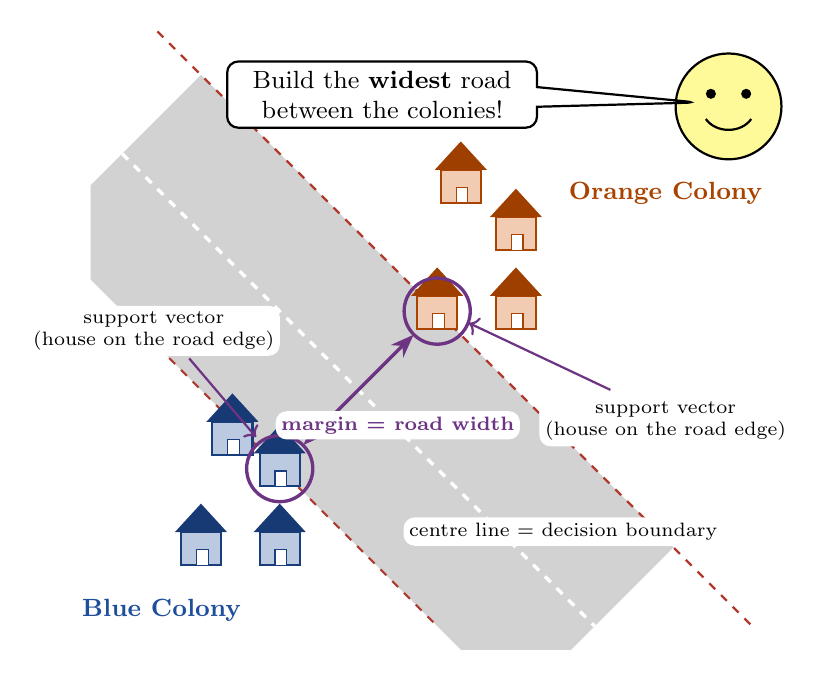
\begin{tikzpicture}
\begin{scope}
\clip (-1.4,-1.3) rectangle (7.6,6.6);
\draw[line width=80.5pt,gray!35] (-1,5)--(5,-1);
\draw[white,dashed,very thick] (-1,5)--(5,-1);
\draw[mlred,dashed,thick] (-1,3)--(3,-1);
\draw[mlred,dashed,thick] (-1,7)--(7,-1);
\end{scope}
\foreach \x/\y in {0/0,1/0,0.4/1.4}  \pic[scale=1.5] at (\x,\y) {house=mlblue};
\foreach \x/\y in {4/4,4/3,3.3/4.6} \pic[scale=1.5] at (\x,\y) {house=mlorange};
\pic[scale=1.5] at (1,1) {house=mlblue};
\pic[scale=1.5] at (3,3) {house=mlorange};
\draw[mlpurple,very thick] (1,1) circle (0.42);
\draw[mlpurple,very thick] (3,3) circle (0.42);
\draw[{Stealth}-{Stealth},very thick,mlpurple] (1.3,1.3)--(2.7,2.7);
\node[font=\scriptsize\bfseries,mlpurple,fill=white,inner sep=2pt,rounded corners] at (2.5,1.55) {margin = road width};
\node[font=\small\bfseries,mlblue] at (-0.5,-0.8) {Blue Colony};
\node[font=\small\bfseries,mlorange!80!black] at (5.9,4.5) {Orange Colony};
\node[font=\scriptsize,align=center,fill=white,rounded corners,inner sep=2pt] at (-0.6,2.75) {support vector\\(house on the road edge)};
\draw[->,thick,mlpurple] (-0.15,2.4)--(0.7,1.4);
\node[font=\scriptsize,align=center,fill=white,rounded corners,inner sep=2pt] at (5.9,1.6) {support vector\\(house on the road edge)};
\draw[->,thick,mlpurple] (5.2,2.0)--(3.4,2.85);
\node[font=\scriptsize,fill=white,rounded corners,inner sep=2pt] at (4.6,0.2) {centre line = decision boundary};
\pic[scale=1.6] at (6.7,5.6) {smile};
\bubble[text width=3.7cm]{2.3,5.75}{6.3,5.65}{Build the \textbf{widest} road between the colonies!}
\end{tikzpicture}}
\caption{A cartoon of the maximum-margin classifier: the widest road between two colonies.}\label{fig:road}
\end{figure}

\begin{explain}
\textbf{Houses} are data points: blue houses are one class and orange houses are the other. The \textbf{grey road} is the margin and the \textbf{white dashed centre line} is the decision boundary. The \textbf{red dashed lines} are the edges of the road.

\medskip
The two \textbf{purple circled houses} sit exactly on the edge of the road. They are the \textbf{support vectors}. If you moved or removed any \emph{other} house (without letting it cross the edge) the road would stay exactly where it is; but if you moved a circled house, the whole road would shift. The \textbf{purple arrow} shows the road width, the \textbf{margin}, which the SVM tries to make as large as possible. A wide road means the classifier keeps a safe distance from both classes, so new houses (new data) are less likely to be misclassified.
\end{explain}

\subsection{Definitions}

\begin{definition}[: Support Vector Machine (SVM)]
A \textbf{Support Vector Machine} is a supervised learning algorithm that classifies data by finding the \textbf{maximum-margin hyperplane}: the separating hyperplane $\vect w\cdot\vect x+b=0$ that is \emph{farthest} from the closest training points of both classes. With labels $y_i\in\{-1,+1\}$ the \textbf{hard-margin} problem is
\[
  \min_{\vect w,b}\ \tfrac12\|\vect w\|^2\qquad\text{subject to}\qquad y_i(\vect w\cdot\vect x_i+b)\ge1\ \ \text{for all }i,
\]
and a new point is classified by $\hat y=\operatorname{sign}(\vect w\cdot\vect x+b)$.
\end{definition}

\begin{definition}[: Margin and support vectors]
The \textbf{margin} is the width $2/\|\vect w\|$ of the empty strip between the two parallel hyperplanes $\vect w\cdot\vect x+b=\pm1$. The \textbf{support vectors} are the training points that lie \emph{on} these hyperplanes (or, for a soft margin, inside them or on the wrong side); they alone determine $\vect w$ and $b$.
\end{definition}

In Chapter~4 we solved a small SVM by hand. Here is a quick reminder of its answer, which we will reuse: for the spam data the support vectors were $(1,1)$ with $y=-1$ and $(3,3)$ with $y=+1$, giving $\vect w=(0.5,0.5)$, $b=-2$ and margin $2/\|\vect w\|=2.83$.

\subsection{Soft-Margin SVM: Strict and Relaxed Teachers}

Real data usually overlap, so no road can perfectly separate the colonies. A \textbf{soft margin} lets a few houses stand on the road or even on the wrong side, but each such house is fined.

\begin{definition}[: Soft-margin SVM]
Introduce a \textbf{slack variable} $\xi_i\ge0$ for each point that measures how far it violates the margin, and solve
\[
  \min_{\vect w,b,\vect\xi}\ \tfrac12\|\vect w\|^2+C\sum_{i=1}^{n}\xi_i\qquad\text{s.t.}\qquad y_i(\vect w\cdot\vect x_i+b)\ge1-\xi_i,\ \ \xi_i\ge0 .
\]
The hyperparameter $C>0$ controls the trade-off. Equivalently the SVM minimises the \textbf{hinge loss} $\max(0,1-y_if(\vect x_i))$ plus the penalty $\frac1{2C}\|\vect w\|^2$.
\end{definition}

Think of $C$ as the \textbf{strictness of a teacher}.

\begin{itemize}
  \item \textbf{Large $C$ = strict teacher:} ``No student may break the rules!'' The road becomes narrow and twists to avoid every violation: low bias, \emph{high variance}, risk of overfitting.
  \item \textbf{Small $C$ = relaxed teacher:} ``A few mistakes are fine.'' The road stays wide and smooth: higher bias, \emph{low variance}, risk of underfitting.
\end{itemize}

\begin{figure}[!htbp]
\centering
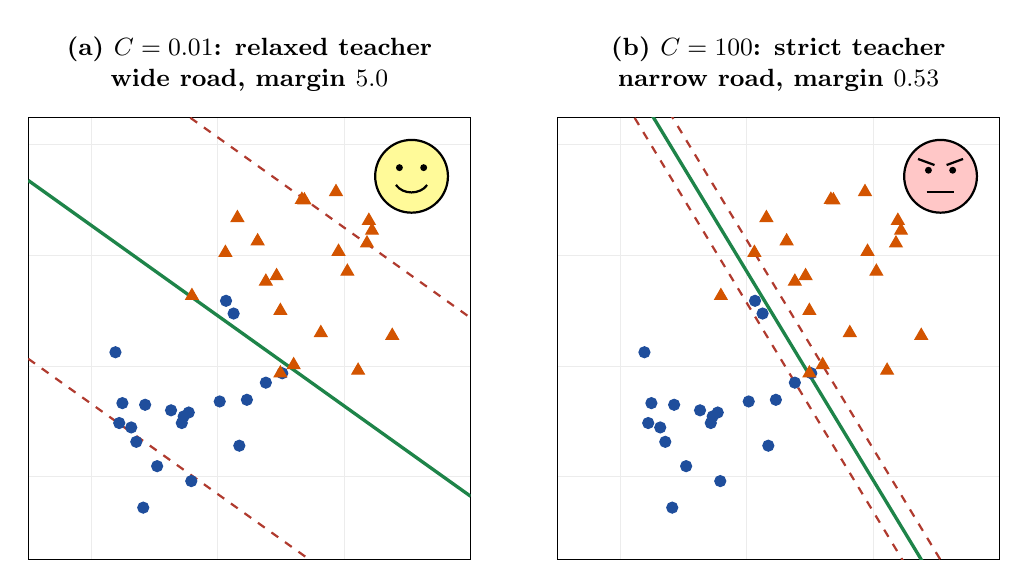
\begin{tikzpicture}
\begin{groupplot}[group style={group size=2 by 1,horizontal sep=1.1cm,group name=G},width=7.2cm,height=7.2cm,
  xmin=-1,xmax=6,ymin=-1.5,ymax=6.5,grid=both,grid style={gray!15},ticks=none,title style={font=\small\bfseries,align=center}]
\nextgroupplot[title={(a) $C=0.01$: relaxed teacher\\wide road, margin $5.0$}]
\addplot[only marks,mark=*,mlblue,mark size=2pt] coordinates {(0.38,2.25)(0.44,0.97)(1.26,1.20)(0.85,1.30)(2.46,1.39)(1.43,0.97)(0.71,0.63)(2.25,2.95)(2.76,1.70)(2.13,3.18)(1.58,-0.08)(3.02,1.87)(0.63,0.89)(1.04,0.19)(0.49,1.33)(1.46,1.09)(1.54,1.16)(2.03,1.36)(2.34,0.56)(0.82,-0.56)};
\addplot[only marks,mark=triangle*,mlorange,mark size=2.6pt] coordinates {(3.87,5.15)(4.39,4.63)(2.76,3.53)(2.63,4.26)(4.05,3.71)(2.99,3.00)(4.76,2.55)(3.37,5.00)(3.20,2.02)(3.63,2.60)(4.36,4.22)(3.91,4.07)(2.31,4.68)(1.59,3.27)(4.44,4.45)(2.99,1.87)(4.22,1.92)(2.93,3.63)(3.33,5.01)(2.12,4.05)};
\addplot[very thick,mlgreen,domain=-1:6]{(1.408-0.253*x)/0.310};
\addplot[dashed,mlred,thick,domain=-1:6]{(2.408-0.253*x)/0.310};
\addplot[dashed,mlred,thick,domain=-1:6]{(0.408-0.253*x)/0.310};
\nextgroupplot[title={(b) $C=100$: strict teacher\\narrow road, margin $0.53$}]
\addplot[only marks,mark=*,mlblue,mark size=2pt] coordinates {(0.38,2.25)(0.44,0.97)(1.26,1.20)(0.85,1.30)(2.46,1.39)(1.43,0.97)(0.71,0.63)(2.25,2.95)(2.76,1.70)(2.13,3.18)(1.58,-0.08)(3.02,1.87)(0.63,0.89)(1.04,0.19)(0.49,1.33)(1.46,1.09)(1.54,1.16)(2.03,1.36)(2.34,0.56)(0.82,-0.56)};
\addplot[only marks,mark=triangle*,mlorange,mark size=2.6pt] coordinates {(3.87,5.15)(4.39,4.63)(2.76,3.53)(2.63,4.26)(4.05,3.71)(2.99,3.00)(4.76,2.55)(3.37,5.00)(3.20,2.02)(3.63,2.60)(4.36,4.22)(3.91,4.07)(2.31,4.68)(1.59,3.27)(4.44,4.45)(2.99,1.87)(4.22,1.92)(2.93,3.63)(3.33,5.01)(2.12,4.05)};
\addplot[very thick,mlgreen,domain=-1:6]{(13.175-3.322*x)/1.761};
\addplot[dashed,mlred,thick,domain=-1:6]{(14.175-3.322*x)/1.761};
\addplot[dashed,mlred,thick,domain=-1:6]{(12.175-3.322*x)/1.761};
\end{groupplot}
\pic[scale=1.1] at ([shift={(-0.75,-0.75)}]G c1r1.north east) {smile};
\pic[scale=1.1] at ([shift={(-0.75,-0.75)}]G c2r1.north east) {angry};
\end{tikzpicture}
\caption{The same 40 points fitted with a very small and a very large $C$ (real SVM fits).}\label{fig:Ceffect}
\end{figure}

\begin{explain}
Both panels show the \emph{same} 40 houses (blue circles and orange triangles; the two colonies overlap a little in the middle). The \textbf{green line} is the decision boundary and the \textbf{red dashed lines} are the road edges.

\medskip
\textbf{(a) Relaxed teacher ($C=0.01$):} the road is very wide (margin $5.0$) and covers many houses, so many of them are support vectors. The model pays little attention to the individual rule-breakers and looks only at the overall pattern.

\textbf{(b) Strict teacher ($C=100$):} the road is narrow (margin $0.53$) and the line is tilted to squeeze between the points, because every violation is expensive. The model follows the training data closely.
\end{explain}

\medskip
\begin{center}
\begin{tabular}{@{}lcccc@{}}
\toprule
\textbf{$C$} & \textbf{Support vectors} & \textbf{Margin} & \textbf{Train accuracy} & \textbf{Test accuracy (400 pts)}\\
\midrule
0.01 (relaxed) & 32 & 5.00 & 0.925 & 0.953\\
1 & 11 & 1.63 & 0.900 & 0.948\\
100 (strict) & 8 & 0.53 & 0.950 & 0.940\\
\bottomrule
\end{tabular}
\end{center}

\textbf{Read the table:} as $C$ grows, the margin shrinks (5.00 $\to$ 0.53), fewer points are support vectors (32 $\to$ 8) and the \emph{training} accuracy rises slightly ($0.925\to0.950$) while the \emph{test} accuracy drifts down ($0.953\to0.940$): the strict teacher fits the training set better but generalises a little worse. (The differences in accuracy are small here, since the two classes are only mildly overlapping and 400 test points is a small sample; the large change in margin and support vectors is the main lesson.)

\subsection{The Dual Form and Support Vectors}

The SVM optimisation problem can be rewritten in an equivalent \emph{dual} form using Lagrange multipliers $\alpha_i\ge0$, one per training point.

\begin{definition}[: Dual form of the SVM]
\[
  \max_{\vect\alpha}\ \sum_{i}\alpha_i-\frac12\sum_{i}\sum_{j}\alpha_i\alpha_j\,y_iy_j\,(\vect x_i\cdot\vect x_j)
  \quad\text{s.t.}\quad \sum_i\alpha_iy_i=0,\ \ 0\le\alpha_i\le C .
\]
The weights are $\vect w=\sum_i\alpha_iy_i\vect x_i$ and a new point is classified by
\[
  f(\vect x)=\sum_{i}\alpha_i\,y_i\,(\vect x_i\cdot\vect x)+b .
\]
Only the \textbf{support vectors} have $\alpha_i>0$; all other points have $\alpha_i=0$.
\end{definition}

\textbf{Two important facts:}
\begin{enumerate}
  \item The prediction needs only the \emph{support vectors}, which makes it compact.
  \item The data enter \emph{only through dot products} $\vect x_i\cdot\vect x_j$. This is the key to the \textbf{kernel trick} in the next section.
\end{enumerate}

\begin{example}[: The dual form on the spam data]
Support vectors: $(1,1)$ with $y=-1$ and $(3,3)$ with $y=+1$; all other points have $\alpha=0$.

\medskip
\textbf{Solving for $\alpha$:} by symmetry $\alpha_1=\alpha_2=\alpha$. Then
\[
  \vect w=\alpha(-1)(1,1)+\alpha(+1)(3,3)=\alpha(2,2)=(0.5,0.5)\ \Rightarrow\ \alpha=0.25 .
\]
Check $\sum\alpha_iy_i=0.25(-1)+0.25(+1)=0$ \checkmark. The bias is $b=-2$ as before.

\medskip
\textbf{Predicting the new e-mail $(4,1)$} using only dot products with the support vectors:
\[
  f=\underbrace{0.25(-1)(1\cdot4+1\cdot1)}_{=-1.25}+\underbrace{0.25(+1)(3\cdot4+3\cdot1)}_{=+3.75}-2=\mathbf{0.5}>0\ \Rightarrow\ \text{spam}.
\]
This matches the value $f(4,1)=0.5$ found in Chapter~4 directly from $\vect w$.

\medskip
\textbf{Dual objective value:} $\sum\alpha_i-\frac12\sum_{i,j}\ldots=0.5-0.25=0.25=\frac12\|\vect w\|^2$, equal to the primal value: the primal and dual give the same answer.
\end{example}

\subsection{Practical Points}

\begin{itemize}
  \item \textbf{Scale the features.} The margin is measured with distances, so a feature with a huge range (salary in rupees) would dominate one with a tiny range (age in years). Standardise first.
  \item \textbf{Choose $C$ by cross-validation} on a grid such as $10^{-2},10^{-1},\dots,10^{3}$.
  \item \textbf{More than two classes:} SVMs are binary. For $K$ classes use \emph{one-vs-rest} ($K$ classifiers, pick the highest score) or \emph{one-vs-one} ($K(K-1)/2$ classifiers that vote).
  \item \textbf{No probabilities by default.} The SVM output $f(\vect x)$ is a signed distance, not a probability (scikit-learn can fit one afterwards with \texttt{probability=True}).
\end{itemize}

\procon{Linear SVM classification}
{\item Wide margin gives good generalisation
 \item Effective with many features (text)
 \item Only support vectors matter, so it is compact
 \item Convex problem: a single global optimum}
{\item No probabilities by default
 \item Needs scaled features
 \item Sensitive to the choice of $C$
 \item Slow for very large datasets
 \item Hard margin fails if classes overlap}
{\item Spam and news-article classification
 \item Handwritten digit recognition
 \item Gene-expression and cancer classification
 \item Image classification}

%====================================================================
\section{Nonlinear SVM Classification}

\subsection{When a Straight Line Is Not Enough}

Many real problems cannot be solved by a straight line. For instance, if the ``blue'' houses are in the \emph{middle} of a village and the ``orange'' houses are all around them, no straight road can separate them.

\begin{figure}[!htbp]
\centering
\resizebox{\linewidth}{!}{%
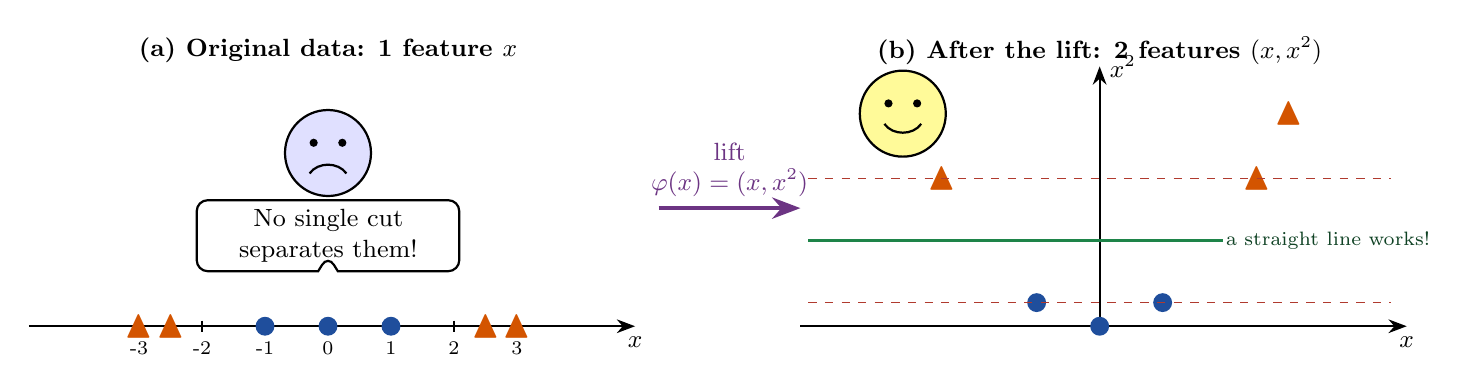
\begin{tikzpicture}
% ---------- left panel : 1-D ----------
\node[font=\small\bfseries] at (2.3,3.5) {(a) Original data: 1 feature $x$};
\draw[-{Stealth},thick] (-1.5,0)--(6.2,0) node[below,font=\small]{$x$};
\foreach \x in {-3,-2,-1,0,1,2,3} \draw (2.3+0.8*\x,0.07)--(2.3+0.8*\x,-0.07) node[below,font=\scriptsize]{\x};
\foreach \x in {-1,0,1} \fill[mlblue] (2.3+0.8*\x,0) circle (0.12);
\foreach \x in {-3,-2.5,2.5,3} \node[mlorange,font=\Large] at (2.3+0.8*\x,0) {$\blacktriangle$};
\pic[scale=1.3] at (2.3,2.2) {sad};
\bubble[text width=3.1cm]{2.3,1.15}{2.3,0.9}{No single cut separates them!}
% arrow between panels
\draw[-{Stealth},ultra thick,mlpurple] (6.5,1.5)--(8.3,1.5) node[midway,above,font=\small,align=center]{lift\\$\varphi(x)=(x,x^2)$};
% ---------- right panel : 2-D ----------
\begin{scope}[xshift=9.8cm]
\node[font=\small\bfseries] at (2.3,3.5) {(b) After the lift: 2 features $(x,x^2)$};
\draw[-{Stealth},thick] (-1.5,0)--(6.2,0) node[below,font=\small]{$x$};
\draw[-{Stealth},thick] (2.3,0)--(2.3,3.3) node[right,font=\small]{$x^2$};
\foreach \x/\y in {-1/1,0/0,1/1} \fill[mlblue] (2.3+0.8*\x,0.3*\y) circle (0.12);
\foreach \x/\y in {-3/9,3/9,-2.5/6.25,2.5/6.25} \node[mlorange,font=\Large] at (2.3+0.8*\x,0.3*\y) {$\blacktriangle$};
\draw[very thick,mlgreen] (-1.4,1.0875)--(6.0,1.0875);
\draw[dashed,mlred] (-1.4,0.3)--(6.0,0.3);
\draw[dashed,mlred] (-1.4,1.875)--(6.0,1.875);
\node[font=\scriptsize,mlgreen!50!black,fill=white,inner sep=1pt] at (5.2,1.0875) {a straight line works!};
\pic[scale=1.3] at (-0.2,2.7) {smile};
\end{scope}
\end{tikzpicture}}
\caption{The lifting trick: data that cannot be separated in one dimension become separable after adding the feature $x^2$.}\label{fig:lift}
\end{figure}

\begin{explain}
\textbf{Panel (a):} the data live on a single number line. The blue circles are in the middle ($x=-1,0,1$) and the orange triangles are on both outsides ($x=\pm2.5,\pm3$). Wherever we put \emph{one} cut-point on the line, some blue and some orange end up on the same side. The sad face is right: no straight cut works.

\medskip
\textbf{Panel (b):} we \emph{lift} every point into two dimensions by adding the new feature $x^2$ (the purple arrow). A point $x=3$ becomes $(3,9)$, and $x=1$ becomes $(1,1)$. Now the orange points have large $x^2$ values and the blue points have small ones, so a \emph{horizontal straight line} (green) separates them perfectly, with red dashed lines marking the margin. Going back to the original line, this horizontal cut corresponds to \emph{two} cut-points, $x\approx-1.9$ and $x\approx+1.9$: a \textbf{nonlinear} boundary in $x$ is a \textbf{linear} boundary in the lifted space.
\end{explain}

\begin{keyidea}
\textbf{A linear model in a higher-dimensional feature space is a nonlinear model in the original space.} The SVM can therefore learn curved boundaries by first mapping the data with a function $\varphi$ and then finding the maximum-margin hyperplane there.
\end{keyidea}

\begin{example}[: Solving the lifted problem end to end]
\textbf{Data:} $x=-1,0,1$ are class $-1$ (blue); $x=\pm2.5,\pm3$ are class $+1$ (orange). Map $\varphi(x)=(x,x^2)$.

\begin{center}
\begin{tabular}{@{}c|ccc|cccc@{}}
\toprule
$x$ & $-1$ & $0$ & $1$ & $-2.5$ & $2.5$ & $-3$ & $3$\\
$\varphi(x)=(x,x^2)$ & $(-1,1)$ & $(0,0)$ & $(1,1)$ & $(-2.5,6.25)$ & $(2.5,6.25)$ & $(-3,9)$ & $(3,9)$\\
Class & $-$ & $-$ & $-$ & $+$ & $+$ & $+$ & $+$\\
\bottomrule
\end{tabular}
\end{center}

\textbf{Step 1: closest opposite points.} In the lifted space the blue points $(\pm1,1)$ have $x^2=1$ and the orange points $(\pm2.5,6.25)$ have $x^2=6.25$. These four are the support vectors. The separating line is horizontal, $\vect w=(0,a)$.

\medskip
\textbf{Step 2: margin conditions.} $a(6.25)+b=+1$ and $a(1)+b=-1$. Subtracting, $5.25\,a=2$ so
\[
  a=0.381,\qquad b=-1-0.381=-1.381,\qquad f(x)=0.381\,x^2-1.381 .
\]

\textbf{Step 3: boundary.} $f(x)=0\iff x^2=3.625\iff x=\pm1.90$. The margin is $2/0.381=5.25$ units in the $x^2$ direction.

\medskip
\textbf{Step 4: check the others.} $f(0)=-1.381\le-1$ \checkmark; $f(\pm3)=0.381(9)-1.381=2.05\ge1$ \checkmark.

\medskip
\textbf{Step 5: predict.} $x=2$: $f=0.381(4)-1.381=0.143>0\Rightarrow$ \textbf{orange}. $x=1.5$: $f=0.381(2.25)-1.381=-0.524<0\Rightarrow$ \textbf{blue}.
\end{example}

\paragraph{The cost of lifting.} Adding more and more features (polynomial features of degree 3, 10, \dots) quickly produces an enormous number of columns: $d$ features and degree $p$ give about $\binom{d+p}{p}$ new features. Computing with them directly becomes very slow. The \textbf{kernel trick} avoids this cost.

\subsection{The Kernel Trick}

Remember that the dual SVM uses the data only through dot products $\vect x_i\cdot\vect x_j$. After the lift we would need $\varphi(\vect x_i)\cdot\varphi(\vect x_j)$. A kernel computes that number \emph{without ever building} $\varphi$.

\begin{definition}[: Kernel function]
A \textbf{kernel} is a function $K(\vect a,\vect b)$ that equals a dot product in some (possibly very high-dimensional) feature space: $K(\vect a,\vect b)=\varphi(\vect a)\cdot\varphi(\vect b)$. The \textbf{kernel trick} replaces every dot product $\vect x_i\cdot\vect x_j$ in the SVM by $K(\vect x_i,\vect x_j)$, so the SVM works in the high-dimensional space \emph{at the cost of computing a simple formula}:
\[
  f(\vect x)=\sum_i\alpha_i\,y_i\,K(\vect x_i,\vect x)+b .
\]
\end{definition}

\begin{center}
\begin{tabular}{@{}p{3.1cm}p{5.5cm}p{4.9cm}@{}}
\toprule
\textbf{Kernel} & \textbf{Formula} & \textbf{Parameters}\\
\midrule
Linear & $K(\vect a,\vect b)=\vect a\cdot\vect b$ & none\\
Polynomial & $K(\vect a,\vect b)=(\gamma\,\vect a\cdot\vect b+r)^{d}$ & degree $d$, $\gamma$, $r$\\
RBF (Gaussian) & $K(\vect a,\vect b)=\exp\!\big(-\gamma\|\vect a-\vect b\|^2\big)$ & $\gamma>0$\\
Sigmoid & $K(\vect a,\vect b)=\tanh(\gamma\,\vect a\cdot\vect b+r)$ & $\gamma$, $r$\\
\bottomrule
\end{tabular}
\end{center}

\begin{example}[: The polynomial kernel really equals a dot product]
Let $\vect a=(1,2)$ and $\vect b=(3,1)$ and take the kernel $K(\vect a,\vect b)=(\vect a\cdot\vect b)^2$.

\medskip
\textbf{Using the kernel (one cheap step):} $\vect a\cdot\vect b=3+2=5$, so $K=5^2=\mathbf{25}$.

\medskip
\textbf{Using the explicit feature map} $\varphi(\vect x)=(x_1^2,\ \sqrt2\,x_1x_2,\ x_2^2)$ (three features):
\[
  \varphi(\vect a)=(1,\ 2.828,\ 4),\qquad \varphi(\vect b)=(9,\ 4.243,\ 1),
\]
\[
  \varphi(\vect a)\cdot\varphi(\vect b)=1(9)+2.828(4.243)+4(1)=9+12+4=\mathbf{25}.
\]
Both ways give $25$, but the kernel never needed the three-dimensional vectors.
\end{example}

\begin{example}[: The RBF kernel as a similarity score]
For $\vect a=(1,2)$ and $\vect b=(3,1)$: $\|\vect a-\vect b\|^2=2^2+1^2=5$.
\begin{center}
\begin{tabular}{@{}lccc@{}}
\toprule
$\gamma$ & $0.1$ & $0.5$ & $2$\\
\midrule
$K=e^{-5\gamma}$ & $e^{-0.5}=0.607$ & $e^{-2.5}=0.082$ & $e^{-10}=0.00005$\\
\bottomrule
\end{tabular}
\end{center}
Also $K(\vect a,\vect a)=e^{0}=1$ (identical points are maximally similar). The RBF kernel is a \textbf{similarity between $0$ and $1$} that falls as the points move apart, and $\gamma$ says \emph{how fast}. The feature space of the RBF kernel has infinitely many dimensions, yet each $K$ is one cheap calculation.
\end{example}

\begin{figure}[!htbp]
\centering
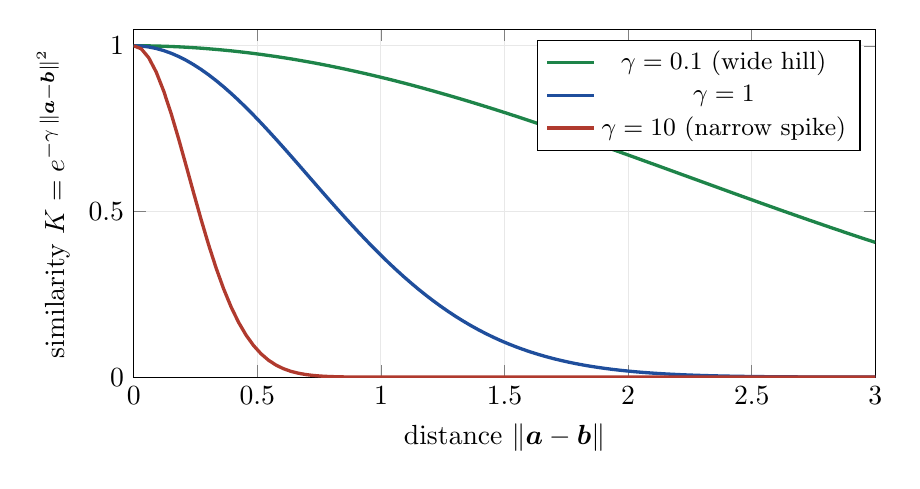
\begin{tikzpicture}
\begin{axis}[width=11cm,height=6cm,xlabel={distance $\|\vect a-\vect b\|$},ylabel={similarity $K=e^{-\gamma\,\|\vect a-\vect b\|^2}$},
  xmin=0,xmax=3,ymin=0,ymax=1.05,samples=100,grid=both,grid style={gray!18},
  legend style={at={(0.98,0.97)},anchor=north east,font=\small}]
\addplot[very thick,mlgreen,domain=0:3]{exp(-0.1*x^2)};
\addplot[very thick,mlblue,domain=0:3]{exp(-1*x^2)};
\addplot[very thick,mlred,domain=0:3]{exp(-10*x^2)};
\legend{$\gamma=0.1$ (wide hill),$\gamma=1$,$\gamma=10$ (narrow spike)}
\end{axis}
\end{tikzpicture}
\caption{The RBF kernel as a function of distance, for three values of $\gamma$.}\label{fig:rbfgamma}
\end{figure}

\begin{explain}
The horizontal axis is the \textbf{distance} between two points and the vertical axis is their \textbf{similarity} (1 = identical, 0 = completely unrelated). Each curve is a different $\gamma$.

\begin{itemize}
  \item \textbf{Green ($\gamma=0.1$):} a wide, gentle hill. Even points that are $2$ units apart are still considered fairly similar. Every training point influences a large neighbourhood, so the model is \emph{smooth} (risk of underfitting).
  \item \textbf{Blue ($\gamma=1$):} a medium hill.
  \item \textbf{Red ($\gamma=10$):} a narrow spike. Only points very close together are similar. Each training point influences just its immediate surroundings, so the boundary becomes wiggly and tightly follows the data (risk of overfitting).
\end{itemize}
\end{explain}

\subsection{How an RBF SVM Decides: Hills of Influence}

Here is a cartoon way to see the RBF-kernel SVM. Each support vector builds a \textbf{hill of influence} around itself: a positive hill for an orange support vector (it ``pulls'' nearby points to the orange class) and a negative hill (a pit) for a blue one. The decision value $f(\vect x)$ at any point is the \emph{sum} of all the hills and pits there.

\begin{figure}[!htbp]
\centering
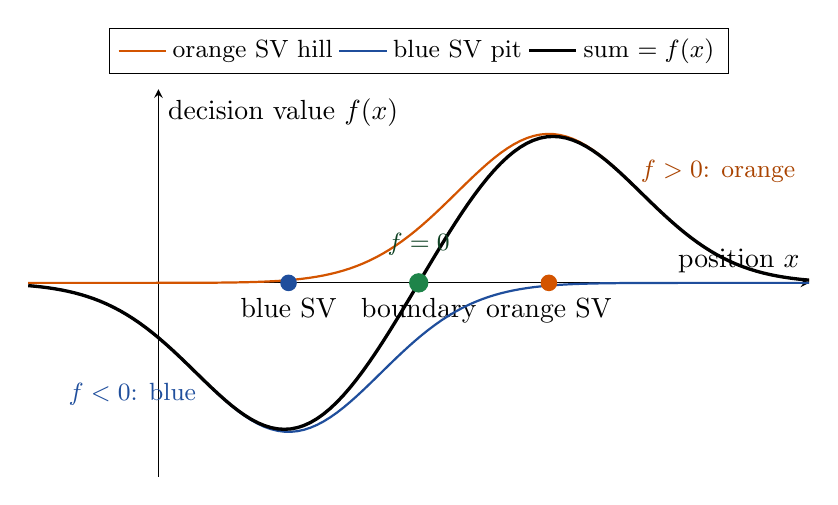
\begin{tikzpicture}
\begin{axis}[width=11.5cm,height=6.5cm,xlabel={position $x$},ylabel={decision value $f(x)$},
  xmin=-1,xmax=5,ymin=-1.3,ymax=1.3,samples=120,axis lines=middle,
  legend style={at={(0.5,1.04)},anchor=south,legend columns=3,font=\small},xtick={1,2,3},xticklabels={blue SV,boundary,orange SV},ytick=\empty]
\addplot[thick,mlorange,domain=-1:5]{exp(-(x-3)^2)};
\addplot[thick,mlblue,domain=-1:5]{-exp(-(x-1)^2)};
\addplot[very thick,black,domain=-1:5]{exp(-(x-3)^2)-exp(-(x-1)^2)};
\legend{orange SV hill,blue SV pit,sum $=f(x)$}
\fill[mlblue] (axis cs:1,0) circle (3pt);
\fill[mlorange] (axis cs:3,0) circle (3pt);
\fill[mlgreen] (axis cs:2,0) circle (3.5pt);
\node[font=\small,mlgreen!50!black,above] at (axis cs:2,0.12) {$f=0$};
\node[font=\small,mlorange!80!black] at (axis cs:4.3,0.75) {$f>0$: orange};
\node[font=\small,mlblue] at (axis cs:-0.2,-0.75) {$f<0$: blue};
\end{axis}
\end{tikzpicture}
\caption{Hills of influence: two RBF support vectors ($\gamma=1$) and the resulting decision value.}\label{fig:hills}
\end{figure}

\begin{explain}
We work in one dimension for clarity, with one blue support vector at $x=1$ and one orange at $x=3$.

\begin{itemize}
  \item The \textbf{orange curve} is the positive hill $e^{-(x-3)^2}$ centred on the orange support vector.
  \item The \textbf{blue curve} is the negative pit $-e^{-(x-1)^2}$ centred on the blue support vector.
  \item The \textbf{black curve} is their sum, the decision value $f(x)$. It is positive on the right (the orange hill wins), negative on the left (the blue pit wins), and crosses \textbf{zero at $x=2$} (green dot), exactly midway, where both influences are equal.
\end{itemize}
In more dimensions it is the same picture: the decision boundary is where the hills and pits cancel, which can be a curve of any shape.
\end{explain}

\subsection{Choosing $C$ and $\gamma$: Real Results}

We trained RBF SVMs on the \texttt{moons} data (two interleaving half-circles with noise): 180 points to train and 120 to test.

\begin{center}
\begin{tabular}{@{}ccccl@{}}
\toprule
\textbf{$\gamma$} & \textbf{Train accuracy} & \textbf{Test accuracy} & \textbf{Support vectors} & \textbf{Diagnosis}\\
\midrule
0.1 & 0.839 & 0.867 & 79 & too smooth: underfits\\
1 & 0.950 & \textbf{0.992} & 54 & good\\
10 & 0.961 & 0.975 & 115 & starting to overfit\\
100 & \textbf{1.000} & 0.850 & 173 & overfits (memorises)\\
\bottomrule
\end{tabular}
\end{center}

\begin{center}
\begin{tabular}{@{}ccc@{\qquad\qquad}ccc@{}}
\toprule
\textbf{$C$} ($\gamma=1$) & \textbf{Train} & \textbf{Test} & \textbf{Kernel} ($C=1$) & \textbf{Train} & \textbf{Test}\\
\midrule
0.1 & 0.928 & 0.950 & Linear & 0.817 & 0.883\\
1 & 0.950 & \textbf{0.992} & Polynomial (degree 3) & 0.944 & 0.983\\
10 & 0.950 & 0.975 & RBF & 0.950 & \textbf{0.992}\\
1000 & 0.967 & 0.933 & & &\\
\bottomrule
\end{tabular}
\end{center}

\textbf{Interpretation.} (i)~With $\gamma=100$ the training accuracy is a perfect $1.000$ but the test accuracy falls to $0.850$: the classic overfitting signature. (ii)~Too small a $\gamma$ underfits. (iii)~Very large $C$ (1000) also overfits ($0.967$ train, $0.933$ test). (iv)~On this curved data the linear SVM is clearly worse ($0.883$) than the polynomial and RBF kernels. (Test accuracies are based on 120 points, so one point is $0.8\%$.)

\begin{tryit}
Reproduce the experiment with \texttt{scikit-learn}:
\begin{lstlisting}
from sklearn.datasets import make_moons
from sklearn.model_selection import train_test_split
from sklearn.preprocessing import StandardScaler
from sklearn.pipeline import make_pipeline
from sklearn.svm import SVC

X, y = make_moons(n_samples=300, noise=0.25, random_state=0)
Xa, Xb, ya, yb = train_test_split(X, y, test_size=0.4,
                                  random_state=0)

for g in [0.1, 1, 10, 100]:
    model = make_pipeline(StandardScaler(),
                          SVC(kernel="rbf", gamma=g, C=1))
    model.fit(Xa, ya)
    print(g, model.score(Xa, ya), model.score(Xb, yb))
\end{lstlisting}
\emph{Challenge:} replace the loop by \texttt{GridSearchCV} over $C\in\{0.1,1,10,100\}$ and $\gamma\in\{0.1,1,10\}$ and report the best pair.
\end{tryit}

\begin{figure}[!htbp]
\centering
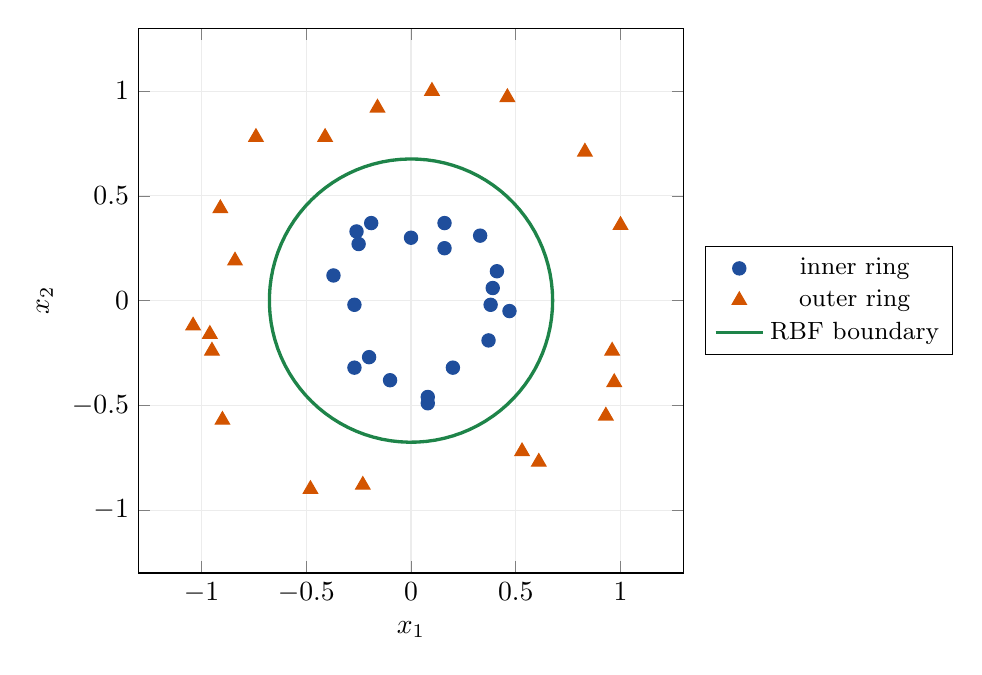
\begin{tikzpicture}
\begin{axis}[width=8.5cm,height=8.5cm,axis equal image,xmin=-1.3,xmax=1.3,ymin=-1.3,ymax=1.3,grid=both,grid style={gray!15},
  xlabel={$x_1$},ylabel={$x_2$},legend style={at={(1.04,0.5)},anchor=west,font=\small}]
\addplot[only marks,mark=*,mlblue,mark size=2.4pt] coordinates {(0.16,0.25)(0.38,-0.02)(0.16,0.37)(0.37,-0.19)(-0.19,0.37)(0.47,-0.05)(-0.26,0.33)(0.33,0.31)(-0.37,0.12)(-0.27,-0.32)(0.39,0.06)(-0.20,-0.27)(-0.25,0.27)(0.08,-0.49)(0.20,-0.32)(0.41,0.14)(-0.10,-0.38)(0.08,-0.46)(0.00,0.30)(-0.27,-0.02)};
\addlegendentry{inner ring}
\addplot[only marks,mark=triangle*,mlorange,mark size=3pt] coordinates {(0.61,-0.77)(0.97,-0.39)(-0.74,0.78)(1.00,0.36)(-0.23,-0.88)(0.83,0.71)(-0.41,0.78)(0.10,1.00)(-0.84,0.19)(0.96,-0.24)(-0.90,-0.57)(0.93,-0.55)(-1.04,-0.12)(0.46,0.97)(-0.96,-0.16)(-0.48,-0.90)(-0.16,0.92)(-0.91,0.44)(0.53,-0.72)(-0.95,-0.24)};
\addlegendentry{outer ring}
\addplot[very thick,mlgreen,domain=0:360,samples=100,variable=\t]({0.676*cos(t)},{0.676*sin(t)});
\addlegendentry{RBF boundary}
\end{axis}
\end{tikzpicture}
\caption{An RBF SVM separates two concentric rings that no straight line can (a real fit, 20 points of each class shown).}\label{fig:circles}
\end{figure}

\begin{explain}
The blue circles form an \textbf{inner ring} and the orange triangles an \textbf{outer ring}. A straight line cannot separate them: a linear SVM got only $58\%$ of these points right. The \textbf{RBF SVM} ($\gamma=2$, $C=10$) classified all of them correctly, and its decision boundary (green) is an almost perfect \textbf{circle of radius $\approx0.68$} lying in the gap between the rings. The curved boundary was never specified by us: the kernel allowed the SVM to find it.
\end{explain}

\begin{keyidea}
\textbf{Choosing a kernel:} start with a \emph{linear} kernel (fast, good for many features and text). If the data look nonlinear, try the \emph{RBF} kernel, which is a good default, and tune $C$ and $\gamma$ by cross-validation on \emph{scaled} features. Use a polynomial kernel when you believe interactions between features of a known degree matter.
\end{keyidea}

\procon{Nonlinear (kernel) SVM}
{\item Learns nonlinear boundaries without building features by hand
 \item Flexible: many kernels
 \item Works well in high dimensions
 \item Strong generalisation with the margin}
{\item Needs careful tuning of $C$, $\gamma$ and the kernel
 \item Training cost grows roughly as $n^2$ to $n^3$: slow for $n\gg10^5$
 \item Hard to interpret
 \item Needs feature scaling}
{\item Face and object recognition
 \item Handwritten digit recognition
 \item Protein and DNA classification
 \item Remote-sensing image classification}

%====================================================================
\section{SVM Regression}

\subsection{The Idea: Points Inside the Tunnel Are Free}

The SVM idea also works for \textbf{regression}. In classification we wanted a road that keeps points \emph{off} the road. In SVM regression we reverse it: we fit a \textbf{tunnel} (tube) around the regression line and try to get \textbf{as many points as possible inside}. Points inside the tunnel cost nothing; only points \emph{outside} are penalised.

\begin{definition}[: $\varepsilon$-insensitive loss]
\[
  L_\varepsilon(y,f(\vect x))=\max\big(0,\ |y-f(\vect x)|-\varepsilon\big).
\]
Errors smaller than $\varepsilon$ are ignored (loss $0$); larger errors cost the amount \emph{by which they exceed $\varepsilon$}.
\end{definition}

\begin{definition}[: Support vector regression (SVR)]
\textbf{SVR} fits a function $f(\vect x)=\vect w\cdot\vect x+b$ (or its kernelised version) that is as \emph{flat} as possible while keeping most training points within a tube of half-width $\varepsilon$:
\[
  \min_{\vect w,b,\vect\xi,\vect\xi^*}\ \tfrac12\|\vect w\|^2+C\sum_i(\xi_i+\xi_i^*)
  \quad\text{s.t.}\quad
  \begin{cases}y_i-f(\vect x_i)\le\varepsilon+\xi_i\\ f(\vect x_i)-y_i\le\varepsilon+\xi_i^*\\ \xi_i,\xi_i^*\ge0.\end{cases}
\]
The slack variables $\xi_i,\xi_i^*$ measure how far a point lies above or below the tube. The \textbf{support vectors} are the points on or outside the tube; points strictly inside have no influence. With a kernel the prediction is $f(\vect x)=\sum_i(\alpha_i-\alpha_i^*)K(\vect x_i,\vect x)+b$.
\end{definition}

\begin{figure}[!htbp]
\centering
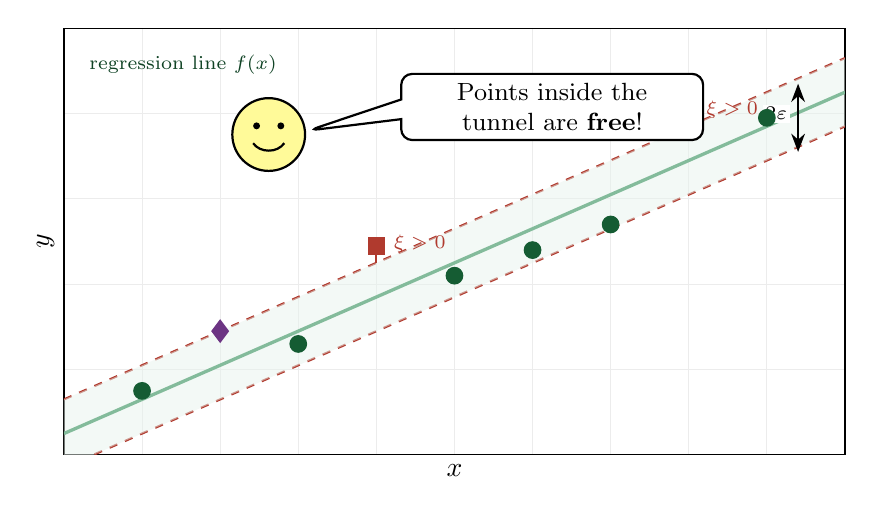
\begin{tikzpicture}
\begin{axis}[width=11.5cm,height=7cm,xlabel={$x$},ylabel={$y$},xmin=0,xmax=10,ymin=0,ymax=10,grid=both,grid style={gray!15},ticks=none]
\addplot[dashed,mlred,thick,domain=0:10]{0.8*x+0.5+0.8};
\addplot[dashed,mlred,thick,domain=0:10]{0.8*x+0.5-0.8};
\addplot[very thick,mlgreen,domain=0:10]{0.8*x+0.5};
\fill[mlgreen!10,opacity=0.5] (axis cs:0,0.5-0.8+0) -- (axis cs:10,8.5-0.8+0) -- (axis cs:10,8.5+0.8) -- (axis cs:0,0.5+0.8) -- cycle;
\addplot[only marks,mark=*,mlgreen!70!black,mark size=3pt] coordinates {(1,1.5)(3,2.6)(5,4.2)(6,4.8)(7,5.4)(9,7.9)};
\addplot[only marks,mark=square*,mlred,mark size=3pt] coordinates {(4,4.9)(8,8.0)};
\addplot[only marks,mark=diamond*,mlpurple,mark size=4pt] coordinates {(2,2.9)};
\draw[mlred,thick] (axis cs:4,4.5)--(axis cs:4,4.9);
\draw[mlred,thick] (axis cs:8,7.7)--(axis cs:8,8.0);
\node[font=\scriptsize,mlred,anchor=west] at (axis cs:4.1,4.95) {$\xi>0$};
\node[font=\scriptsize,mlred,anchor=west] at (axis cs:8.1,8.1) {$\xi>0$};
\draw[{Stealth}-{Stealth},thick] (axis cs:9.4,7.1)--(axis cs:9.4,8.7);
\node[font=\scriptsize,anchor=east,fill=white,inner sep=1pt] at (axis cs:9.3,8.0) {$2\varepsilon$};
\node[font=\scriptsize,mlgreen!50!black,anchor=north west] at (axis cs:0.2,9.6) {regression line $f(x)$};
\end{axis}
\pic[scale=1.1] at ([shift={(2.6,-1.35)}]current axis.north west) {smile};
\bubble[text width=3.6cm]{$(current axis.north west)+(6.2,-1.0)$}{$(current axis.north west)+(3.1,-1.3)$}{Points inside the tunnel are \textbf{free}!}
\end{tikzpicture}
\caption{Support vector regression: a tube of half-width $\varepsilon$ around the fitted line.}\label{fig:svr}
\end{figure}

\begin{explain}
The \textbf{green line} is the fitted regression function and the \textbf{red dashed lines} are the tube edges, a distance $\varepsilon$ above and below the line (total width $2\varepsilon$).

\begin{itemize}
  \item The \textbf{green dots} lie \emph{inside} the tunnel. Their errors are smaller than $\varepsilon$, so they cost nothing and \emph{do not affect} the line at all (they are not support vectors).
  \item The \textbf{red squares} lie \emph{outside} the tunnel. They are penalised by the distance $\xi$ to the nearest tube edge (the short red segments). They are support vectors.
  \item The \textbf{purple diamond} sits exactly on the tube edge and is also a support vector.
\end{itemize}
A wider tunnel (large $\varepsilon$) includes more points, gives a simpler model and fewer support vectors; a narrow tunnel follows the data more closely.
\end{explain}

\begin{example}[: The $\varepsilon$-insensitive loss]
Let $\varepsilon=0.5$. Three predictions:

\begin{center}
\begin{tabular}{@{}c|ccc|c@{}}
\toprule
 & \textbf{Point 1} & \textbf{Point 2} & \textbf{Point 3} & \textbf{Total}\\
\midrule
True $y$ & 3.0 & 4.1 & 6.5 & \\
Predicted $f$ & 3.3 & 4.0 & 5.2 & \\
Error $y-f$ & $-0.3$ & $0.1$ & $1.3$ & \\
\midrule
$L_\varepsilon=\max(0,|e|-0.5)$ & $0$ & $0$ & $0.8$ & $\mathbf{0.8}$\\
Squared error $e^2$ & $0.09$ & $0.01$ & $1.69$ & $1.79$\\
\bottomrule
\end{tabular}
\end{center}
Points 1 and 2 lie inside the tube and are \emph{ignored}; only point~3 is charged ($1.3-0.5=0.8$). Ordinary squared error would have charged all three points.
\end{example}

\subsection{Real Results}

We fitted noisy data from $y=\sin x$ (60 points: 42 train, 18 test).

\begin{center}
\begin{tabular}{@{}lccc@{}}
\toprule
\textbf{Model} & \textbf{Train $R^2$} & \textbf{Test $R^2$} & \textbf{Support vectors}\\
\midrule
Linear SVR & 0.539 & 0.278 & 39\\
RBF SVR ($C=10,\gamma=1,\varepsilon=0.1$) & \textbf{0.971} & \textbf{0.924} & 26\\
\bottomrule
\end{tabular}
\end{center}

\begin{center}
\begin{tabular}{@{}cccl@{}}
\toprule
\textbf{$\varepsilon$} (RBF SVR) & \textbf{Support vectors} & \textbf{Test $R^2$} & \textbf{Comment}\\
\midrule
0.05 & 35 & 0.914 & narrow tube, many support vectors\\
0.2 & 17 & \textbf{0.942} & good balance\\
0.5 & 4 & 0.841 & tube too wide: underfits\\
\bottomrule
\end{tabular}
\end{center}

\textbf{Read the tables.} A straight line cannot follow the sine curve ($R^2=0.28$ on test data), while the RBF kernel can ($0.92$). Widening the tube from $0.05$ to $0.5$ reduces the number of support vectors from $35$ to $4$, but when the tube is too wide the fit gets worse.

\begin{tryit}
\begin{lstlisting}
import numpy as np
from sklearn.svm import SVR
from sklearn.model_selection import train_test_split

rng = np.random.default_rng(0)
x = np.sort(rng.uniform(0, 6, 60))
y = np.sin(x) + rng.normal(0, 0.15, 60)
xa, xb, ya, yb = train_test_split(x.reshape(-1, 1), y,
                                  test_size=0.3, random_state=0)

svr = SVR(kernel="rbf", C=10, gamma=1, epsilon=0.1).fit(xa, ya)
print(svr.score(xa, ya), svr.score(xb, yb), len(svr.support_))
\end{lstlisting}
\emph{Challenge:} try \texttt{epsilon=0.3} and \texttt{gamma=10} and compare the train and test $R^2$.
\end{tryit}

\begin{center}
\begin{tabular}{@{}p{3.6cm}p{4.9cm}p{5.2cm}@{}}
\toprule
\textbf{Parameter} & \textbf{Meaning} & \textbf{Effect when increased}\\
\midrule
$\varepsilon$ & Half-width of the tube & Fewer support vectors, simpler (flatter) model\\
$C$ & Penalty for points outside the tube & Fits training data more closely (overfits)\\
$\gamma$ (RBF) & Reach of each support vector & More wiggly curve (overfits)\\
\bottomrule
\end{tabular}
\end{center}

\procon{SVM regression (SVR)}
{\item Ignores small errors, so robust to noise
 \item Sparse: only support vectors matter
 \item Nonlinear fits through kernels
 \item Good generalisation}
{\item Three parameters to tune ($\varepsilon$, $C$, $\gamma$)
 \item Slow for very large datasets
 \item Needs feature scaling
 \item No probabilistic prediction interval}
{\item Stock and sales forecasting
 \item Electricity-load and weather prediction
 \item Estimating material or engineering properties
 \item Travel-time estimation}

%====================================================================
\section{Naive Bayes Classifiers}

In Chapter~3 we introduced Bayes' theorem and the Naive Bayes classifier. Here we study the three main \emph{variants}, one for each type of feature, and solve a full text-classification example. First recall the principle.

\begin{definition}[: Naive Bayes classifier]
A \textbf{Naive Bayes classifier} predicts the class
\[
  \hat y=\argmax_{c}\ P(c)\prod_{j=1}^{d}P(x_j\mid c),
\]
where the ``naive'' assumption is that the features are \emph{conditionally independent given the class}. It is a \textbf{generative} classifier: it models how each class generates the data, $P(\vect x\mid c)$, and then uses Bayes' theorem to get $P(c\mid\vect x)$.
\end{definition}

\subsection{The Detective Who Multiplies Clues}

Think of the classifier as a \textbf{detective}. Each feature is a \emph{clue}. The detective does not worry about how the clues are connected (the naive assumption); each clue is allowed to ``speak'' separately, and the detective \textbf{multiplies the votes} of all clues together with the prior suspicion.

\begin{figure}[!htbp]
\centering
\resizebox{\linewidth}{!}{%
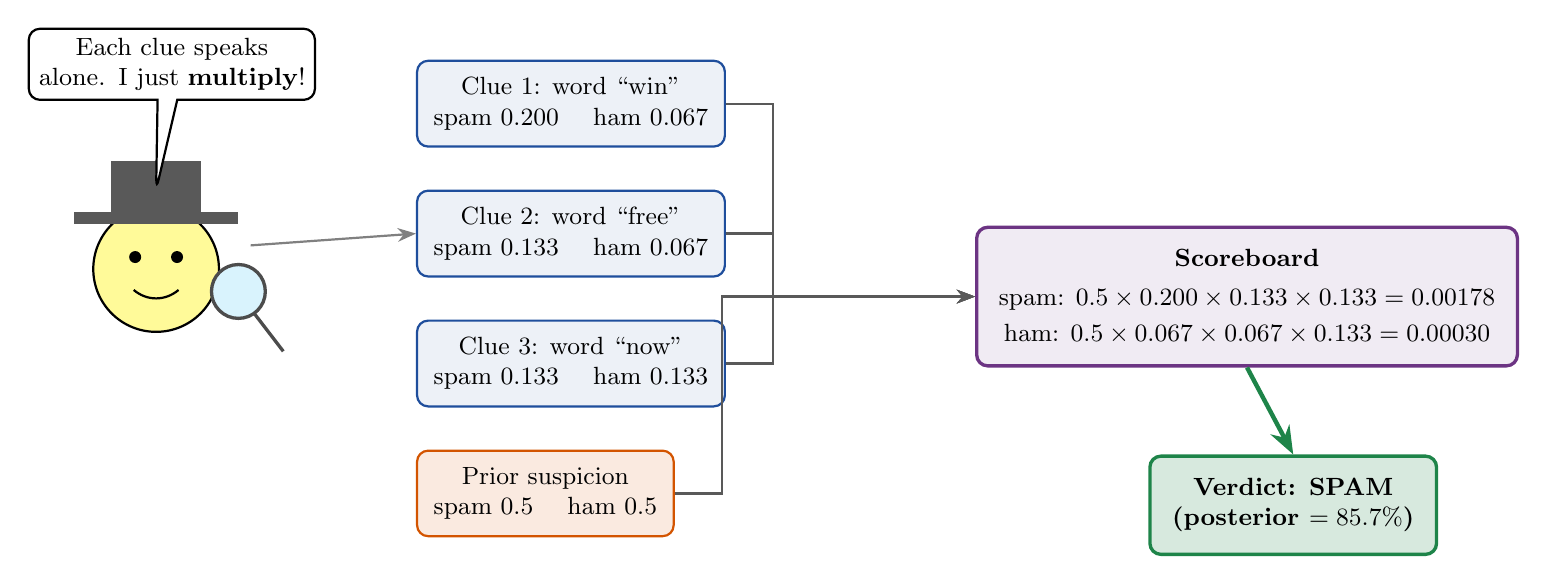
\begin{tikzpicture}[card/.style={draw,rounded corners,thick,fill=mlblue!8,draw=mlblue,align=center,font=\small,inner sep=6pt,anchor=west}]
\pic[scale=1.9] at (0,0) {detective};
\bubble[text width=3.4cm]{0.2,2.6}{0,1.0}{Each clue speaks alone. I just \textbf{multiply}!}
\node[card] (c1) at (3.3,2.1) {Clue 1: word ``win''\\spam $0.200$ \quad ham $0.067$};
\node[card] (c2) at (3.3,0.45) {Clue 2: word ``free''\\spam $0.133$ \quad ham $0.067$};
\node[card] (c3) at (3.3,-1.2) {Clue 3: word ``now''\\spam $0.133$ \quad ham $0.133$};
\node[card,fill=mlorange!12,draw=mlorange] (pr) at (3.3,-2.85) {Prior suspicion\\spam $0.5$ \quad ham $0.5$};
\node[draw,rounded corners,very thick,fill=mlpurple!10,draw=mlpurple,align=center,font=\small,inner sep=8pt,anchor=west] (sc) at (10.4,-0.35) {\textbf{Scoreboard}\\[3pt]spam: $0.5\times0.200\times0.133\times0.133=0.00178$\\[2pt]ham: $0.5\times0.067\times0.067\times0.133=0.00030$};
\node[draw,rounded corners,very thick,fill=mlgreen!18,draw=mlgreen,align=center,font=\small\bfseries,inner sep=8pt,anchor=west] (vd) at (12.6,-3.0) {Verdict: SPAM\\(posterior $=85.7\%$)};
\foreach \c in {c1,c2,c3,pr} \draw[-{Stealth},thick,gray!70!black] (\c.east)--++(0.6,0) |- (sc.west);
\draw[-{Stealth},ultra thick,mlgreen] (sc.south)--(vd.north);
\draw[-{Stealth},thick,gray] (1.2,0.3)--(c2.west);
\end{tikzpicture}}
\caption{Naive Bayes as a detective: the evidence of each word is multiplied with the prior.}\label{fig:detective}
\end{figure}

\begin{explain}
The detective is examining the message ``\textbf{win free now}''. The three blue cards are the clues, each giving how likely the word is under \emph{spam} and under \emph{ham} (probabilities estimated from a tiny training set, worked out in detail below). The orange card is the prior: before reading the message we think spam and ham are equally likely. The \textbf{purple scoreboard} multiplies the prior with each clue. Spam scores $0.00178$ and ham only $0.00030$, so the \textbf{verdict is spam}. The word ``win'' is the strongest clue because it is three times more likely in spam; the word ``now'' is no help at all (equal probability), so it simply cancels out.
\end{explain}

\subsection{Gaussian Naive Bayes (continuous features)}

\begin{definition}[: Gaussian Naive Bayes]
For \textbf{continuous} features, $P(x_j\mid c)$ is modelled by a normal density with a \emph{class-specific} mean $\mu_{jc}$ and variance $\sigma_{jc}^2$ estimated from the training data of class $c$:
\[
  P(x_j\mid c)=\frac{1}{\sqrt{2\pi}\,\sigma_{jc}}\exp\!\Big(-\frac{(x_j-\mu_{jc})^2}{2\sigma_{jc}^2}\Big).
\]
\end{definition}

\textbf{Real-life example: ripe or unripe mango.} A fruit seller measures the \emph{sweetness score} and the \emph{colour} of mangoes. From past data: ripe mangoes have sweetness $\sim\mathcal N(6,1)$ and are yellow with probability $0.9$; unripe mangoes have sweetness $\sim\mathcal N(3,1)$ and are yellow with probability $0.2$. Both classes are equally common.

\begin{figure}[!htbp]
\centering
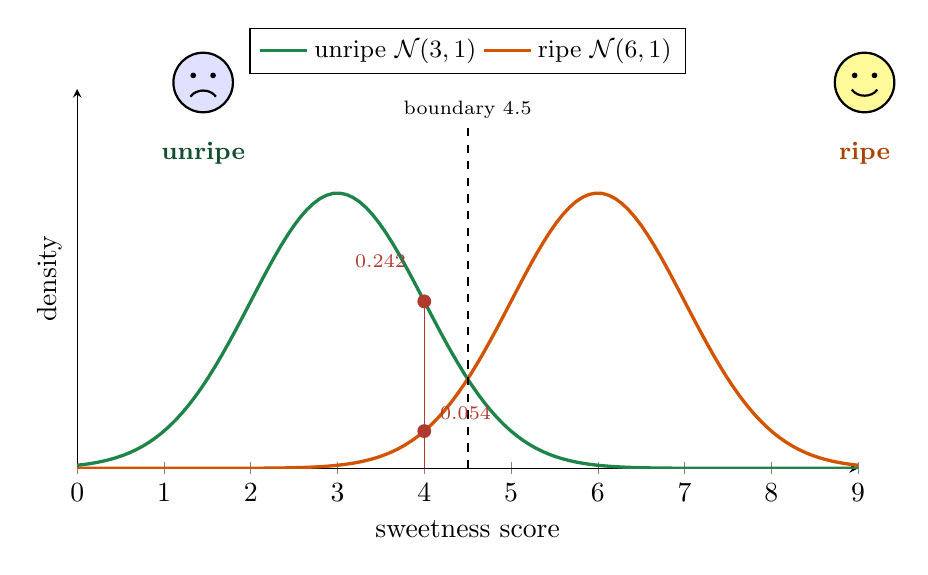
\begin{tikzpicture}
\begin{axis}[width=11.5cm,height=6.4cm,xlabel={sweetness score},ylabel={density},xmin=0,xmax=9,ymin=0,ymax=0.55,samples=120,axis lines=left,ytick=\empty,
  legend style={at={(0.5,1.04)},anchor=south,legend columns=2,font=\small}]
\addplot[very thick,mlgreen,domain=0:9]{exp(-(x-3)^2/2)/sqrt(2*pi)};
\addplot[very thick,mlorange,domain=0:9]{exp(-(x-6)^2/2)/sqrt(2*pi)};
\legend{{unripe $\mathcal N(3,1)$},{ripe $\mathcal N(6,1)$}}
\draw[dashed,thick] (axis cs:4.5,0)--(axis cs:4.5,0.5);
\node[font=\scriptsize,fill=white,inner sep=1pt] at (axis cs:4.5,0.52) {boundary $4.5$};
\fill[mlred] (axis cs:4,0.242) circle (2.5pt); \fill[mlred] (axis cs:4,0.054) circle (2.5pt);
\draw[mlred,thin] (axis cs:4,0) -- (axis cs:4,0.242);
\node[font=\scriptsize,mlred,anchor=east] at (axis cs:3.9,0.30) {$0.242$};
\node[font=\scriptsize,mlred,anchor=west] at (axis cs:4.07,0.08) {$0.054$};
\end{axis}
\pic[scale=0.9] at ([shift={(10.0,4.9)}]current axis.south west) {smile};
\node[font=\small\bfseries,mlorange!80!black] at ([shift={(10.0,4.0)}]current axis.south west) {ripe};
\pic[scale=0.9] at ([shift={(1.6,4.9)}]current axis.south west) {sad};
\node[font=\small\bfseries,mlgreen!60!black] at ([shift={(1.6,4.0)}]current axis.south west) {unripe};
\end{tikzpicture}
\caption{Class-conditional densities of sweetness for ripe and unripe mangoes (Gaussian Naive Bayes in one dimension).}\label{fig:mango}
\end{figure}

\begin{explain}
Each bell curve shows how sweetness is distributed in one class: unripe mangoes cluster around $3$ (green) and ripe ones around $6$ (orange). The curves cross at $4.5$, halfway between the means: with equal priors, a mango sweeter than $4.5$ is classified ripe and a less sweet one unripe. For a mango of sweetness $4$ (red dots) the unripe curve is higher ($0.242$) than the ripe curve ($0.054$), so the model leans towards \emph{unripe}.
\end{explain}

\begin{example}[: Mango classification, one feature]
A mango has sweetness $x=4$. Equal priors $0.5$ each.
\begin{align*}
  P(4\mid\text{ripe})&=\tfrac{1}{\sqrt{2\pi}}\,e^{-(4-6)^2/2}=0.3989\,e^{-2}=0.0540,\\
  P(4\mid\text{unripe})&=\tfrac{1}{\sqrt{2\pi}}\,e^{-(4-3)^2/2}=0.3989\,e^{-0.5}=0.2420 .
\end{align*}
\[
  P(\text{ripe}\mid x=4)=\frac{0.5(0.0540)}{0.5(0.0540)+0.5(0.2420)}=\frac{0.0540}{0.2960}=\mathbf{0.182}\ \Rightarrow\ \text{unripe}.
\]
\textbf{Effect of the prior.} If ripe mangoes were four times as common (priors $0.8$ ripe, $0.2$ unripe): $P(\text{ripe}\mid x=4)=\frac{0.8(0.0540)}{0.8(0.0540)+0.2(0.2420)}=\frac{0.0432}{0.0916}=0.472$, much closer to $0.5$. A strong prior can move the decision.
\end{example}

\begin{example}[: Mango classification, two features (sweetness and colour)]
A mango has sweetness $4.8$ and is \textbf{yellow}. Equal priors.

\medskip
\begin{center}
\begin{tabular}{@{}lcc@{}}
\toprule
\textbf{Quantity} & \textbf{Ripe} & \textbf{Unripe}\\
\midrule
Prior $P(c)$ & $0.5$ & $0.5$\\
$P(\text{sweetness}=4.8\mid c)$ (Gaussian) & $\varphi(-1.2)=0.1942$ & $\varphi(1.8)=0.0790$\\
$P(\text{yellow}\mid c)$ & $0.9$ & $0.2$\\
\midrule
\textbf{Score} $=P(c)\prod P(x_j\mid c)$ & $0.5(0.1942)(0.9)=0.0874$ & $0.5(0.0790)(0.2)=0.0079$\\
\bottomrule
\end{tabular}
\end{center}
\[
  P(\text{ripe}\mid\text{data})=\frac{0.0874}{0.0874+0.0079}=\mathbf{0.917}\ \Rightarrow\ \text{ripe}.
\]
\textbf{Teamwork of the clues:} sweetness $4.8$ alone is a moderately ripe-looking value ($P=0.1942/(0.1942+0.0790)=0.71$), and the yellow colour makes it much more convincing ($0.917$).
\end{example}

\subsection{Multinomial Naive Bayes (word counts)}

\begin{definition}[: Multinomial Naive Bayes]
For \textbf{count data} such as word counts in a document, a class $c$ is described by a probability $P(w\mid c)$ for each word $w$ in the vocabulary of size $V$. With Laplace smoothing $\alpha$,
\[
  P(w\mid c)=\frac{N_{wc}+\alpha}{N_c+\alpha V},
\]
where $N_{wc}$ is the number of times word $w$ appears in training documents of class $c$ and $N_c$ is the total number of word occurrences in class $c$. A document with words $w_1,\dots,w_m$ is scored by $P(c)\prod_{k=1}^{m}P(w_k\mid c)$.
\end{definition}

\textbf{Real-life example: spam or ham SMS.} A tiny training set of four messages:

\begin{center}
\begin{tabular}{@{}lll@{}}
\toprule
\textbf{Message} & \textbf{Class} & \textbf{Words}\\
\midrule
``win cash now'' & spam & win, cash, now\\
``win free prize'' & spam & win, free, prize\\
``meet me now'' & ham & meet, me, now\\
``lunch with me'' & ham & lunch, with, me\\
\bottomrule
\end{tabular}
\end{center}

\begin{example}[: Multinomial Naive Bayes, end to end]
\textbf{Step 1: priors.} 2 spam and 2 ham messages: $P(\text{spam})=P(\text{ham})=0.5$.

\medskip
\textbf{Step 2: counts.} The vocabulary has $V=9$ words: cash, free, lunch, me, meet, now, prize, win, with. Each class has $N_c=6$ word occurrences.

\medskip
\textbf{Step 3: smoothed probabilities} with $\alpha=1$, so every denominator is $6+9=15$:

\begin{center}
\small
\begin{tabular}{@{}l|ccccccccc@{}}
\toprule
\textbf{Word} & win & cash & now & free & prize & meet & me & lunch & with\\
\midrule
Count in spam & 2 & 1 & 1 & 1 & 1 & 0 & 0 & 0 & 0\\
$P(w\mid\text{spam})$ & $\frac3{15}$ & $\frac2{15}$ & $\frac2{15}$ & $\frac2{15}$ & $\frac2{15}$ & $\frac1{15}$ & $\frac1{15}$ & $\frac1{15}$ & $\frac1{15}$\\
\midrule
Count in ham & 0 & 0 & 1 & 0 & 0 & 1 & 2 & 1 & 1\\
$P(w\mid\text{ham})$ & $\frac1{15}$ & $\frac1{15}$ & $\frac2{15}$ & $\frac1{15}$ & $\frac1{15}$ & $\frac2{15}$ & $\frac3{15}$ & $\frac2{15}$ & $\frac2{15}$\\
\bottomrule
\end{tabular}
\end{center}

\medskip
\textbf{Step 4: classify ``win free now''.}
\begin{align*}
\text{score(spam)}&=0.5\cdot\tfrac3{15}\cdot\tfrac2{15}\cdot\tfrac2{15}=0.5\cdot\tfrac{12}{3375}=0.001778,\\
\text{score(ham)}&=0.5\cdot\tfrac1{15}\cdot\tfrac1{15}\cdot\tfrac2{15}=0.5\cdot\tfrac{2}{3375}=0.000296 .
\end{align*}
\[
P(\text{spam}\mid\text{message})=\frac{12}{12+2}=\frac{6}{7}=\mathbf{0.857}\ \Rightarrow\ \textbf{spam}.
\]

\medskip
\textbf{Step 5: classify ``meet me now''.} spam: $0.5\cdot\frac1{15}\cdot\frac1{15}\cdot\frac2{15}\to2$ units; ham: $0.5\cdot\frac2{15}\cdot\frac3{15}\cdot\frac2{15}\to12$ units. So $P(\text{ham})=\frac{12}{14}=0.857$: \textbf{ham}.

\medskip
\textbf{Why smoothing matters.} Without smoothing, $P(\text{win}\mid\text{ham})=\frac06=0$, and any message containing ``win'' would get a ham score of exactly $0$, whatever its other words. With $\alpha=1$ it is $\frac1{15}$: small but not zero.
\end{example}

\subsection{Bernoulli Naive Bayes (word present or absent)}

\begin{definition}[: Bernoulli Naive Bayes]
For \textbf{binary} features $x_j\in\{0,1\}$ (word present or absent), each feature has a probability $p_{jc}=P(x_j=1\mid c)$ and
\[
  P(x_j\mid c)=p_{jc}^{\,x_j}(1-p_{jc})^{\,1-x_j},\qquad p_{jc}=\frac{n_{jc}+\alpha}{N_c^{\text{docs}}+2\alpha},
\]
where $n_{jc}$ is the number of documents of class $c$ containing feature $j$. Unlike the multinomial model, it \emph{explicitly uses the absence of a word} as evidence.
\end{definition}

\begin{example}[: Bernoulli Naive Bayes on the same messages]
Each class has $2$ documents, so $p_{jc}=\frac{n_{jc}+1}{4}$.

\begin{center}
\small
\begin{tabular}{@{}l|ccccccccc@{}}
\toprule
\textbf{Word} & win & cash & now & free & prize & meet & me & lunch & with\\
\midrule
$P(\text{present}\mid\text{spam})$ & $0.75$ & $0.5$ & $0.5$ & $0.5$ & $0.5$ & $0.25$ & $0.25$ & $0.25$ & $0.25$\\
$P(\text{present}\mid\text{ham})$ & $0.25$ & $0.25$ & $0.5$ & $0.25$ & $0.25$ & $0.5$ & $0.75$ & $0.5$ & $0.5$\\
\bottomrule
\end{tabular}
\end{center}

\medskip
Classify ``win free now'': present words win, free, now; \textbf{absent} words cash, prize, meet, me, lunch, with.
\begin{align*}
\text{spam:}\ & 0.5\times\underbrace{0.75\cdot0.5\cdot0.5}_{\text{present}}\times\underbrace{0.5\cdot0.5\cdot0.75\cdot0.75\cdot0.75\cdot0.75}_{\text{absent}}=0.01483,\\
\text{ham:}\ & 0.5\times\underbrace{0.25\cdot0.25\cdot0.5}_{\text{present}}\times\underbrace{0.75\cdot0.75\cdot0.5\cdot0.25\cdot0.5\cdot0.5}_{\text{absent}}=0.00055 .
\end{align*}
$P(\text{spam})=\dfrac{0.01483}{0.01483+0.00055}=\mathbf{0.964}$: spam, with an even higher confidence than the multinomial model, because the \emph{absence} of ham-typical words (me, meet, lunch, with) is also evidence.
\end{example}

\begin{center}
\begin{tabular}{@{}p{2.8cm}p{3.2cm}p{3.6cm}p{3.9cm}@{}}
\toprule
\textbf{Variant} & \textbf{Feature type} & \textbf{Models $P(x_j\mid c)$ by} & \textbf{Typical use}\\
\midrule
Gaussian & Continuous measurements & Normal density per class & Medical measurements, sensors\\
Multinomial & Counts (word counts, frequencies) & Word probabilities with smoothing & Text classification, spam\\
Bernoulli & Binary (present/absent) & Presence probability per feature & Short texts, binary indicators\\
\bottomrule
\end{tabular}
\end{center}

\begin{tryit}
Confirm the hand calculations with \texttt{scikit-learn}:
\begin{lstlisting}
from sklearn.feature_extraction.text import CountVectorizer
from sklearn.naive_bayes import MultinomialNB, BernoulliNB

docs = ["win cash now", "win free prize", "meet me now",
        "lunch with me"]
labels = [1, 1, 0, 0]                      # 1 = spam, 0 = ham

cv = CountVectorizer(binary=False)
mnb = MultinomialNB(alpha=1).fit(cv.fit_transform(docs), labels)
print(mnb.predict_proba(cv.transform(["win free now"])))
# -> [[0.143 0.857]]   P(ham), P(spam)

cvb = CountVectorizer(binary=True)
bnb = BernoulliNB(alpha=1).fit(cvb.fit_transform(docs), labels)
print(bnb.predict_proba(cvb.transform(["win free now"])))
# -> [[0.036 0.964]]
\end{lstlisting}
The outputs, $0.857$ (multinomial) and $0.964$ (Bernoulli) for ``spam'', agree with the hand calculation.
\end{tryit}

\subsection{Generative vs.\ Discriminative Classifiers}

\begin{center}
\begin{tabular}{@{}p{3.4cm}p{5.2cm}p{5.2cm}@{}}
\toprule
 & \textbf{Naive Bayes (generative)} & \textbf{Logistic regression / SVM (discriminative)}\\
\midrule
What is learned & $P(\vect x\mid c)$ and $P(c)$ & $P(c\mid\vect x)$ or the boundary directly\\
Training & Counting; very fast & Optimisation; slower\\
Data needed & Works with little data & Needs more data, but usually more accurate with plenty\\
Feature dependence & Assumed independent & Can use correlated features\\
Probabilities & Often over-confident & Logistic: better calibrated\\
\bottomrule
\end{tabular}
\end{center}

\begin{warning}
Naive Bayes often classifies well even when its probabilities are \emph{wrong}. If the posterior says $0.999$, do not trust that number literally: the independence assumption multiplies correlated evidence several times and makes the model over-confident. Use it to \emph{rank} or \emph{decide}, not to quote exact probabilities.
\end{warning}

\procon{Naive Bayes classifiers}
{\item Extremely fast to train and predict
 \item Works with little training data and many features
 \item Handles multiple classes naturally
 \item Excellent baseline for text}
{\item Independence assumption is rarely true
 \item Probabilities over-confident
 \item Zero-frequency problem (needs smoothing)
 \item Cannot learn feature interactions}
{\item Spam filtering and sentiment analysis
 \item News and document categorisation
 \item Medical diagnosis (Gaussian)
 \item Real-time prediction}

%====================================================================
\section{Comparing the Methods of Unit~III}

\begin{center}
\small
\begin{tabular}{@{}p{3.2cm}p{3.6cm}p{3.4cm}p{3.6cm}@{}}
\toprule
 & \textbf{Kernel SVM} & \textbf{Naive Bayes} & \textbf{Random Forest / Boosting}\\
\midrule
Training speed & Slow for large $n$ & \textbf{Very fast} & Moderate\\
Prediction speed & Fast (few support vectors) & \textbf{Very fast} & Moderate\\
Nonlinear? & Yes (kernel) & Mild & \textbf{Yes}\\
Needs scaling? & \textbf{Yes} & No & No\\
Probabilities? & Not directly & Yes (over-confident) & Yes\\
Works with little data & Yes & \textbf{Yes} & Less so\\
Interpretability & Low & Moderate & Low--moderate\\
\end{tabular}
\end{center}

%====================================================================
\begin{summary}
\begin{itemize}
  \item \textbf{Linear SVM:} the maximum-margin hyperplane; margin $2/\|\vect w\|$; support vectors lie on the road edge and alone determine the model.
  \item \textbf{Soft margin:} slack $\xi_i$ and parameter $C$; large $C$ = strict (narrow margin, overfit), small $C$ = relaxed (wide margin, underfit).
  \item \textbf{Dual form:} $f(\vect x)=\sum\alpha_iy_i(\vect x_i\cdot\vect x)+b$; only support vectors have $\alpha_i>0$; data appear only through dot products.
  \item \textbf{Nonlinear SVM:} lift the data with $\varphi$; the \textbf{kernel trick} replaces dot products by $K(\vect a,\vect b)=\varphi(\vect a)\cdot\varphi(\vect b)$. Polynomial: $(\gamma\vect a\cdot\vect b+r)^d$; RBF: $e^{-\gamma\|\vect a-\vect b\|^2}$. Large $\gamma$ or $C$ overfits.
  \item \textbf{SVR:} $\varepsilon$-tube; loss $\max(0,|y-f|-\varepsilon)$; points inside the tube are free; support vectors are on or outside.
  \item \textbf{Naive Bayes:} $\hat y=\argmax_cP(c)\prod_jP(x_j\mid c)$; Gaussian (continuous), multinomial (counts), Bernoulli (binary); use Laplace smoothing $\frac{N_{wc}+\alpha}{N_c+\alpha V}$.
  \item Worked results: SVM lifted boundary at $x=\pm1.90$; RBF kernel $e^{-0.5\cdot5}=0.082$; SMS ``win free now'' spam with $0.857$ (multinomial) and $0.964$ (Bernoulli); mango ripe with $0.917$.
\end{itemize}
\end{summary}

%====================================================================
\section*{Exam Corner}
\addcontentsline{toc}{section}{Exam Corner}

\subsection*{A.\ Very Short Answer Questions (2 marks each)}
\begin{enumerate}
  \item Define a support vector machine. \qmarks{2}
  \item What are support vectors? What is the margin? \qmarks{2}
  \item What is the role of the parameter $C$ in a soft-margin SVM? \qmarks{2}
  \item Write the decision function of an SVM in dual form. \qmarks{2}
  \item What is the kernel trick? \qmarks{2}
  \item Write the formulas of the polynomial and RBF kernels. \qmarks{2}
  \item What does a large $\gamma$ do in the RBF kernel? \qmarks{2}
  \item Define the $\varepsilon$-insensitive loss. \qmarks{2}
  \item What is the effect of increasing $\varepsilon$ in SVR? \qmarks{2}
  \item State the independence assumption of Naive Bayes. \qmarks{2}
  \item What is Laplace smoothing? \qmarks{2}
  \item Name the three types of Naive Bayes and their feature types. \qmarks{2}
\end{enumerate}

\begin{modelans}[: Q5, Q7 and Q9]
\textbf{Q5.} The kernel trick is the replacement of every dot product $\vect x_i\cdot\vect x_j$ in the SVM by a kernel $K(\vect x_i,\vect x_j)=\varphi(\vect x_i)\cdot\varphi(\vect x_j)$. The SVM then works in a high-dimensional feature space without ever computing the mapping $\varphi$, which makes nonlinear classification possible at low cost.\par
\textbf{Q7.} A large $\gamma$ makes the similarity fall off very quickly with distance: every training point influences only a tiny neighbourhood, producing a very wiggly decision boundary. It reduces bias but increases variance, so it \emph{overfits}.\par
\textbf{Q9.} A larger $\varepsilon$ gives a wider tube; more points fall inside, fewer are support vectors, and the model becomes simpler (flatter). If $\varepsilon$ is too large the model underfits.
\end{modelans}

\subsection*{B.\ Short Answer Questions (5 marks each)}
\begin{enumerate}
  \item Explain the maximum-margin classifier and support vectors with a diagram. \qmarks{5}
  \item Explain the soft-margin SVM. Discuss the effect of $C$. \qmarks{5}
  \item Explain the dual form of the SVM and why it is important for kernels. \qmarks{5}
  \item Why do we need nonlinear SVMs? Explain the lifting idea with an example. \qmarks{5}
  \item Explain the kernel trick. Describe the linear, polynomial and RBF kernels. \qmarks{5}
  \item Explain the effect of $C$ and $\gamma$ on an RBF SVM. \qmarks{5}
  \item Explain SVM regression with the $\varepsilon$-tube. \qmarks{5}
  \item Explain the Gaussian, multinomial and Bernoulli Naive Bayes classifiers. \qmarks{5}
  \item Explain why Laplace smoothing is needed in Naive Bayes with an example. \qmarks{5}
  \item Compare generative and discriminative classifiers. \qmarks{5}
\end{enumerate}

\begin{modelans}[: B6 (outline for 5 marks)]
\textbf{Parameter $C$} (penalty for margin violations): large $C$ $\to$ few violations, narrow margin, complex boundary, \emph{low bias, high variance} (overfit); small $C$ $\to$ wide margin, simple boundary, \emph{higher bias, low variance} (underfit).\par
\textbf{Parameter $\gamma$} (reach of each support vector in $e^{-\gamma\|a-b\|^2}$): large $\gamma$ $\to$ narrow influence, wiggly boundary, overfit; small $\gamma$ $\to$ wide influence, smooth boundary, underfit.\par
\textbf{Example:} on the moons data ($\gamma=0.1,1,100$) test accuracy was $0.867,\ 0.992,\ 0.850$ while training accuracy rose to $1.0$ at $\gamma=100$. Both parameters are chosen by cross-validation on scaled features.
\end{modelans}

\subsection*{C.\ Long Answer Questions (10 marks each)}
\begin{enumerate}
  \item Explain linear SVM classification: the margin, the optimisation problem, support vectors, soft margin and the dual form. Solve a small numerical example. \qmarks{10}
  \item Explain nonlinear SVM classification. Describe the kernel trick with the polynomial and RBF kernels, including a numerical verification that $K(\vect a,\vect b)=\varphi(\vect a)\cdot\varphi(\vect b)$. \qmarks{10}
  \item Explain SVM regression: the $\varepsilon$-insensitive loss, the optimisation problem, support vectors and the roles of $\varepsilon$, $C$ and $\gamma$. \qmarks{10}
  \item Explain the Naive Bayes classifier. Classify a message using the multinomial model with Laplace smoothing for a given training set. \qmarks{10}
  \item Describe the Gaussian, multinomial and Bernoulli Naive Bayes classifiers with formulas, examples, advantages and disadvantages. \qmarks{10}
  \item Compare SVM, Naive Bayes and ensemble methods (Random Forest / boosting) for classification. \qmarks{10}
\end{enumerate}

\begin{modelans}[: C2 (numerical verification)]
Take $\vect a=(1,2)$, $\vect b=(3,1)$ and $K(\vect a,\vect b)=(\vect a\cdot\vect b)^2$.\par
\emph{Via the kernel:} $\vect a\cdot\vect b=1(3)+2(1)=5$, $K=25$.\par
\emph{Via the feature map} $\varphi(\vect x)=(x_1^2,\sqrt2x_1x_2,x_2^2)$: $\varphi(\vect a)=(1,2\sqrt2,4)$, $\varphi(\vect b)=(9,3\sqrt2,1)$; $\varphi(\vect a)\cdot\varphi(\vect b)=9+2\sqrt2\cdot3\sqrt2+4=9+12+4=25$.\par
Both give $25$, so the kernel equals the dot product in the 3-D feature space while needing only one 2-D dot product.
\end{modelans}

\subsection*{D.\ Numerical Problems}
\begin{enumerate}
  \item An SVM has $\vect w=(2,1)$, $b=-4$. Classify $(1,1)$ and $(3,2)$ and find the margin. \textit{(Answer: $f(1,1)=-1\Rightarrow-1$ (on the margin); $f(3,2)=4\Rightarrow+1$; margin $=2/\sqrt5=0.894$.)}
  \item In 1-D the support vectors are $x=1$ ($y=-1$) and $x=3$ ($y=+1$). Find $w,b$, the margin and the dual values $\alpha_i$. \textit{(Answer: $w+b=-1$, $3w+b=1\Rightarrow w=1$, $b=-2$; margin $=2$; $w=\sum\alpha_iy_ix_i=3\alpha-\alpha=2\alpha=1\Rightarrow\alpha=0.5$ each; check $\sum\alpha_iy_i=0$.)}
  \item Using the dual weights $\alpha=0.5$ at $x=1$ ($y=-1$) and $x=3$ ($y=+1$) with $b=-2$, compute $f(2.5)$. \textit{(Answer: $0.5(-1)(1\cdot2.5)+0.5(1)(3\cdot2.5)-2=-1.25+3.75-2=0.5>0$.)}
  \item Compute the polynomial kernel $K(\vect a,\vect b)=(\vect a\cdot\vect b+1)^2$ for $\vect a=(1,2)$, $\vect b=(2,1)$. \textit{(Answer: $\vect a\cdot\vect b=4$; $K=25$.)}
  \item Compute the RBF kernel for $\vect a=(1,2)$, $\vect b=(2,1)$ with $\gamma=0.5$. \textit{(Answer: $\|\vect a-\vect b\|^2=2$; $K=e^{-1}=0.368$.)}
  \item With $\varphi(x)=(x,x^2)$ compute $\varphi(2)\cdot\varphi(3)$ and the matching kernel $K(2,3)=2\cdot3+(2\cdot3)^2$. \textit{(Answer: $\varphi(2)\cdot\varphi(3)=(2,4)\cdot(3,9)=6+36=42$; $K=6+36=42$.)}
  \item In SVR with $\varepsilon=0.3$: $y=(2.0,3.0,5.0)$, $f=(2.2,3.5,4.1)$. Find the total $\varepsilon$-insensitive loss. \textit{(Answer: errors $-0.2,-0.5,0.9$; losses $0,0.2,0.6$; total $0.8$.)}
  \item Gaussian NB: ripe $\sim\mathcal N(6,1)$, unripe $\sim\mathcal N(3,1)$, equal priors. Find $P(\text{ripe}\mid x=4)$. \textit{(Answer: densities $0.0540$ and $0.2420$; posterior $0.182$.)}
  \item Using the SMS example, classify ``win now'' with multinomial NB. \textit{(Answer: spam $0.5\cdot\frac3{15}\cdot\frac2{15}=0.01333$; ham $0.5\cdot\frac1{15}\cdot\frac2{15}=0.00444$; $P(\text{spam})=0.75$.)}
  \item A word never occurs in the 200 word-tokens of a class; the vocabulary has 1000 words. Find its Laplace-smoothed probability ($\alpha=1$). \textit{(Answer: $\frac{0+1}{200+1000}=0.00083$.)}
\end{enumerate}

\subsection*{E.\ Multiple-Choice Questions}
\begin{enumerate}
  \item The support vectors of an SVM are: \\
  (a) all training points \quad (b) points on or inside the margin \quad (c) the outliers only \quad (d) the test points
  \item The margin of a linear SVM equals: \\
  (a) $\|\vect w\|$ \quad (b) $1/\|\vect w\|$ \quad (c) $2/\|\vect w\|$ \quad (d) $\|\vect w\|^2$
  \item A very large $C$ in a soft-margin SVM tends to: \\
  (a) widen the margin \quad (b) narrow the margin and overfit \quad (c) remove all support vectors \quad (d) make the model linear
  \item In the dual form the data appear only through: \\
  (a) squares \quad (b) dot products \quad (c) means \quad (d) labels
  \item The RBF kernel is: \\
  (a) $\vect a\cdot\vect b$ \quad (b) $(\vect a\cdot\vect b+1)^2$ \quad (c) $e^{-\gamma\|\vect a-\vect b\|^2}$ \quad (d) $\tanh(\vect a\cdot\vect b)$
  \item A very large $\gamma$ in an RBF SVM leads to: \\
  (a) underfitting \quad (b) overfitting \quad (c) a linear boundary \quad (d) fewer features
  \item In SVR, points strictly inside the $\varepsilon$-tube: \\
  (a) are support vectors \quad (b) have no effect on the model \quad (c) have the largest loss \quad (d) are removed from the data
  \item Increasing $\varepsilon$ in SVR typically: \\
  (a) increases support vectors \quad (b) decreases support vectors \quad (c) changes nothing \quad (d) adds features
  \item Naive Bayes assumes features are: \\
  (a) identical \quad (b) conditionally independent given the class \quad (c) all Gaussian \quad (d) uncorrelated with the class
  \item Which variant suits word counts? \\
  (a) Gaussian \quad (b) Multinomial \quad (c) Linear \quad (d) Sigmoid
  \item Laplace smoothing prevents: \\
  (a) overfitting of trees \quad (b) zero probabilities \quad (c) scaling problems \quad (d) ties
  \item Which classifier is \emph{generative}? \\
  (a) SVM \quad (b) logistic regression \quad (c) Naive Bayes \quad (d) k-NN
\end{enumerate}
\textbf{Answers:} 1-b,\ 2-c,\ 3-b,\ 4-b,\ 5-c,\ 6-b,\ 7-b,\ 8-b,\ 9-b,\ 10-b,\ 11-b,\ 12-c.

\subsection*{F.\ Practice Problems}
\begin{enumerate}
  \item Using the 1-D lifted example, classify $x=-2$ and $x=0.5$ with $f(x)=0.381x^2-1.381$. \textit{(Answer: $f(-2)=0.143\Rightarrow$ orange; $f(0.5)=-1.286\Rightarrow$ blue.)}
  \item Draw the margin and support vectors for the data $(1,1),(2,2)$ in class $-1$ and $(4,4),(5,5)$ in class $+1$. Find $\vect w$, $b$ and the margin. \textit{(Hint: closest pair $(2,2)$ and $(4,4)$.)}
  \item \textbf{Coding:} train \texttt{SVC} with linear, polynomial and RBF kernels on \texttt{make\_circles} and report the accuracies.
  \item \textbf{Coding:} use \texttt{GridSearchCV} to tune $C$ and $\gamma$ of an RBF SVM on the \emph{breast cancer} dataset (after scaling).
  \item \textbf{Coding:} write your own spam examples and train \texttt{MultinomialNB} with \texttt{alpha=1} and \texttt{alpha=0.01}; compare predicted probabilities.
\end{enumerate}

\begin{revision}
\begin{center}\small
\begin{tabular}{@{}p{3.6cm}p{9.6cm}@{}}
\toprule
\textbf{Topic} & \textbf{One-line recall}\\
\midrule
Linear SVM & Max-margin hyperplane; margin $2/\|w\|$; min $\frac12\|w\|^2$ s.t.\ $y_i(w\cdot x_i+b)\ge1$.\\
Support vectors & Points on / inside the margin; only they determine $w,b$.\\
Soft margin & Slack $\xi_i$, penalty $C$: large $C$ strict (overfit), small $C$ relaxed (underfit).\\
Dual form & $f(x)=\sum\alpha_iy_i(x_i\cdot x)+b$; $\alpha_i>0$ only for support vectors.\\
Kernel trick & Replace dot product by $K(a,b)=\varphi(a)\cdot\varphi(b)$.\\
Kernels & Linear $a\cdot b$; poly $(\gamma a\cdot b+r)^d$; RBF $e^{-\gamma\|a-b\|^2}$.\\
$C$, $\gamma$ & Large $C$ / large $\gamma$: overfit; small: underfit.\\
SVR & $\varepsilon$-tube; loss $\max(0,|y-f|-\varepsilon)$; points inside are free.\\
Naive Bayes & $\arg\max_cP(c)\prod_jP(x_j\mid c)$; generative; conditional independence.\\
Variants & Gaussian (continuous), multinomial (counts), Bernoulli (binary).\\
Smoothing & $\frac{N_{wc}+\alpha}{N_c+\alpha V}$ avoids zero probabilities.\\
\bottomrule
\end{tabular}
\end{center}
\end{revision}

\chapter{Clustering: K-Means, DBSCAN and Gaussian Mixtures}

\newcommand{\kmAplot}{\addplot[only marks,mlblue,mark=*,mark size=2.2pt] coordinates {(1.06,-0.37) (0.91,0.49) (1.97,0.35) (0.89,0.43) (1.60,-0.33) (1.90,0.02) (1.89,-0.12) (2.05,0.33) (1.70,-0.09) (1.62,-0.17) (1.92,0.17) (0.51,-0.37) (0.76,-0.55) (1.56,-0.37) (0.62,-0.42) (1.22,-0.52) (0.84,-0.41) (0.87,0.66) (2.03,0.52) (0.98,-0.54) (1.04,0.48) (0.62,-0.43) (1.13,0.09) (0.47,-0.19) (0.94,0.25) (0.66,-0.41) (1.26,-0.36) (2.07,-0.06) (1.75,-0.08) (1.37,-0.46) (0.93,0.02) (1.35,-0.42) (0.95,0.25)};}
\newcommand{\kmBplot}{\addplot[only marks,mlorange,mark=triangle*,mark size=2.8pt] coordinates {(-0.99,0.36) (0.53,0.84) (-0.78,0.45) (0.54,0.88) (0.23,0.26) (0.75,0.76) (0.35,0.96) (0.28,-0.05) (-1.09,0.08) (0.12,0.84) (0.03,0.42) (-0.84,0.60) (-0.13,1.04) (0.63,0.78) (-0.65,0.51) (-0.33,0.86) (0.08,0.39) (-0.97,0.57) (0.18,0.90) (-0.94,0.10) (0.09,-0.00) (-0.47,0.85) (-0.01,1.04) (-0.69,0.74) (0.18,1.00) (0.21,0.08) (-0.85,0.49) (0.23,-0.36) (-0.28,0.90) (-1.03,0.30) (-0.01,0.14) (0.21,-0.05) (0.23,-0.27) (0.74,0.72) (-0.34,0.91) (-0.32,1.02) (-0.61,0.82)};}
\newcommand{\dbAplot}{\addplot[only marks,mlblue,mark=*,mark size=2.2pt] coordinates {(-0.99,0.36) (0.53,0.84) (-0.78,0.45) (0.54,0.88) (0.91,0.49) (0.75,0.76) (0.89,0.43) (0.35,0.96) (-1.09,0.08) (0.12,0.84) (-0.84,0.60) (-0.13,1.04) (0.63,0.78) (-0.65,0.51) (-0.33,0.86) (-0.97,0.57) (0.18,0.90) (0.87,0.66) (-0.94,0.10) (1.04,0.48) (1.13,0.09) (0.94,0.25) (-0.47,0.85) (-0.01,1.04) (-0.69,0.74) (0.18,1.00) (-0.85,0.49) (-0.28,0.90) (-1.03,0.30) (0.74,0.72) (-0.34,0.91) (-0.32,1.02) (0.93,0.02) (0.95,0.25) (-0.61,0.82)};}
\newcommand{\dbBplot}{\addplot[only marks,mlorange,mark=triangle*,mark size=2.8pt] coordinates {(1.06,-0.37) (0.23,0.26) (1.97,0.35) (1.60,-0.33) (1.90,0.02) (0.28,-0.05) (1.89,-0.12) (2.05,0.33) (1.70,-0.09) (0.03,0.42) (1.62,-0.17) (1.92,0.17) (0.51,-0.37) (0.08,0.39) (0.76,-0.55) (1.56,-0.37) (0.62,-0.42) (1.22,-0.52) (0.84,-0.41) (0.98,-0.54) (0.09,-0.00) (0.62,-0.43) (0.47,-0.19) (0.66,-0.41) (0.21,0.08) (0.23,-0.36) (-0.01,0.14) (1.26,-0.36) (2.07,-0.06) (1.75,-0.08) (0.21,-0.05) (1.37,-0.46) (0.23,-0.27) (1.35,-0.42)};}
\newcommand{\dbNplot}{\addplot[only marks,red,mark=x,very thick,mark size=4pt] coordinates {(2.03,0.52)};}

\newcommand{\gmmPAplot}{\addplot[only marks,mlblue,mark=*,mark size=2.2pt] coordinates {(0.06,0.26) (1.50,-1.44) (1.07,-1.12) (0.97,-1.03) (-0.33,0.62) (0.81,-0.55) (1.40,-0.71) (0.81,-0.51) (0.94,-0.50) (1.34,-1.39) (0.95,-0.65) (1.72,-2.15) (-0.51,1.20) (1.28,-1.35) (1.51,-1.59) (0.41,-0.01) (-0.17,1.04) (1.11,-1.47) (0.29,-0.08) (0.72,0.03) (0.71,-0.16) (0.28,-0.09) (0.90,-0.93) (1.88,-2.54) (0.76,-0.24) (0.71,-0.51) (1.80,-2.00) (0.35,0.69) (2.21,-2.66) (1.71,-2.61)};}
\newcommand{\kmPAplot}{\addplot[only marks,mlblue,mark=*,mark size=2.2pt] coordinates {(-2.87,0.68) (-3.05,0.89) (-3.13,1.30) (-2.42,-0.45) (-2.68,0.66) (-2.89,0.73) (-2.62,0.27) (-3.09,1.27) (-3.16,0.88) (-3.56,1.00) (-3.12,1.19) (-1.59,-1.45) (-2.99,0.99) (-2.79,1.29) (-2.53,0.29) (-2.93,0.87) (-2.20,-0.78) (-2.97,0.61) (-2.04,1.71) (-2.27,1.82) (-1.49,1.40) (-1.42,1.42) (-1.62,1.30) (-1.70,1.60) (-1.66,1.46) (-1.44,1.13) (-0.33,0.62) (-0.51,1.20) (-0.17,1.04)};}
\newcommand{\gmmPBplot}{\addplot[only marks,mlorange,mark=triangle*,mark size=2.8pt] coordinates {(-2.87,0.68) (-3.05,0.89) (-3.42,1.92) (-3.91,2.02) (-3.13,1.30) (-2.42,-0.45) (-2.68,0.66) (-3.90,2.12) (-3.98,2.06) (-2.89,0.73) (-2.62,0.27) (-3.09,1.27) (-3.16,0.88) (-3.91,1.70) (-3.56,1.00) (-4.84,3.44) (-3.12,1.19) (-4.81,3.26) (-1.59,-1.45) (-3.80,1.97) (-2.99,0.99) (-4.39,2.54) (-2.79,1.29) (-2.53,0.29) (-4.05,2.54) (-3.98,2.94) (-3.88,2.28) (-2.93,0.87) (-2.20,-0.78) (-2.97,0.61)};}
\newcommand{\kmPBplot}{\addplot[only marks,mlorange,mark=triangle*,mark size=2.8pt] coordinates {(-3.42,1.92) (-3.91,2.02) (-3.90,2.12) (-3.98,2.06) (-3.91,1.70) (-4.84,3.44) (-4.81,3.26) (-3.80,1.97) (-4.39,2.54) (-4.05,2.54) (-3.98,2.94) (-3.88,2.28) (-2.42,2.29) (-3.18,3.74) (-4.06,5.17) (-3.84,3.61) (-3.67,3.90) (-3.26,4.04) (-2.91,3.62) (-2.93,3.08) (-2.93,2.84) (-2.92,3.48) (-3.94,5.08) (-3.11,3.44) (-2.95,2.90) (-3.28,4.09) (-3.29,3.63) (-3.75,4.15) (-2.70,2.82) (-2.60,2.44) (-2.54,3.00) (-3.06,3.68) (-2.08,2.51) (-2.91,2.94)};}
\newcommand{\gmmPCplot}{\addplot[only marks,mlgreen,mark=square*,mark size=2.2pt] coordinates {(-2.42,2.29) (-3.18,3.74) (-4.06,5.17) (-3.84,3.61) (-2.04,1.71) (-2.27,1.82) (-3.67,3.90) (-1.49,1.40) (-1.42,1.42) (-3.26,4.04) (-2.91,3.62) (-2.93,3.08) (-2.93,2.84) (-2.92,3.48) (-1.62,1.30) (-1.70,1.60) (-1.66,1.46) (-3.94,5.08) (-3.11,3.44) (-2.95,2.90) (-3.28,4.09) (-3.29,3.63) (-3.75,4.15) (-2.70,2.82) (-2.60,2.44) (-1.44,1.13) (-2.54,3.00) (-3.06,3.68) (-2.08,2.51) (-2.91,2.94)};}
\newcommand{\kmPCplot}{\addplot[only marks,mlgreen,mark=square*,mark size=2.2pt] coordinates {(0.06,0.26) (1.50,-1.44) (1.07,-1.12) (0.97,-1.03) (0.81,-0.55) (1.40,-0.71) (0.81,-0.51) (0.94,-0.50) (1.34,-1.39) (0.95,-0.65) (1.72,-2.15) (1.28,-1.35) (1.51,-1.59) (0.41,-0.01) (1.11,-1.47) (0.29,-0.08) (0.72,0.03) (0.71,-0.16) (0.28,-0.09) (0.90,-0.93) (1.88,-2.54) (0.76,-0.24) (0.71,-0.51) (1.80,-2.00) (0.35,0.69) (2.21,-2.66) (1.71,-2.61)};}
\newcommand{\ellAplot}{\addplot[thick,mlblue!80!black,domain=0:360,samples=80,variable=\t] ({0.987+2*0.193*cos(t)*-0.5479-2*1.238*sin(t)*0.8365},{-0.814+2*0.193*cos(t)*0.8365+2*1.238*sin(t)*-0.5479});}
\newcommand{\ellBplot}{\addplot[thick,mlorange!80!black,domain=0:360,samples=80,variable=\t] ({-3.300+2*0.181*cos(t)*-0.5535-2*1.395*sin(t)*0.8329},{1.225+2*0.181*cos(t)*0.8329+2*1.395*sin(t)*-0.5535});}
\newcommand{\ellCplot}{\addplot[thick,mlgreen!60!black,domain=0:360,samples=80,variable=\t] ({-2.683+2*0.210*cos(t)*-0.5587-2*1.319*sin(t)*0.8294},{2.903+2*0.210*cos(t)*0.8294+2*1.319*sin(t)*-0.5587});}
\newcommand{\kmcentersplot}{\addplot[only marks,mark=star,black,mark size=5pt,very thick] coordinates {(-2.38,0.82) (-3.36,3.13) (1.11,-0.98)};}


\begin{objectives}
After studying this chapter you will be able to:
\begin{itemize}
  \item define \textbf{clustering} and explain how it differs from classification;
  \item run the \textbf{K-Means} algorithm by hand, explain \textbf{inertia}, \textbf{K-Means++} and how to choose $k$ with the \textbf{elbow} and \textbf{silhouette} methods;
  \item explain the \textbf{limits of K-Means} and recognise when it fails;
  \item use clustering for \textbf{image segmentation}, \textbf{preprocessing} and \textbf{semi-supervised learning};
  \item explain \textbf{DBSCAN} (core, border and noise points) and apply it to a small dataset by hand;
  \item explain \textbf{Gaussian mixture models}, the \textbf{EM algorithm} and \textbf{soft clustering}, and carry out an EM step by hand;
  \item choose between K-Means, DBSCAN and GMM;
  \item answer 2-, 5- and 10-mark university questions on this part of Unit~IV.
\end{itemize}
\end{objectives}

\begin{pullquote}[--- a data scientist's saying]
Supervised learning answers ``which of the known groups is this?'' Clustering answers ``are there any groups at all?''
\end{pullquote}

%====================================================================
\section{Introduction to Clustering}

Imagine you pour a bag of mixed socks onto the floor. Nobody tells you the categories, but you quickly start making piles: black socks here, white socks there, striped socks over there. You have just \textbf{clustered} the socks, using only how similar they look.

\begin{definition}[: Clustering]
\textbf{Clustering} is an \emph{unsupervised} learning task: given unlabelled data $\{\vect{x}_i\}_{i=1}^n$, divide it into groups (\textbf{clusters}) so that instances in the \emph{same} cluster are \emph{similar} to each other and instances in \emph{different} clusters are \emph{dissimilar}. There are no correct labels to learn from; the groups are discovered from the structure of the data.
\end{definition}

\paragraph{Clustering is not classification.}
\begin{center}
\begin{tabular}{@{}p{3.3cm}p{5.5cm}p{5.5cm}@{}}
\toprule
 & \textbf{Classification} & \textbf{Clustering}\\
\midrule
Labels in training data? & Yes (supervised) & No (unsupervised)\\
Groups known beforehand? & Yes, fixed classes & No, discovered from data\\
Goal & Predict the class of a new item & Find natural groups\\
Evaluation & Accuracy against true labels & Cohesion/separation measures\\
Example & Spam or not spam & Group customers by buying habits\\
\bottomrule
\end{tabular}
\end{center}

\paragraph{Why cluster?}
\begin{itemize}
  \item \textbf{Customer segmentation:} group shoppers so that each group gets a suitable offer.
  \item \textbf{Image segmentation:} split a picture into regions (Section~\ref{sec:seg}).
  \item \textbf{Anomaly detection:} points that belong to no cluster are suspicious.
  \item \textbf{Data exploration and compression:} summarise millions of points by a few cluster centres.
  \item \textbf{Helping other learning tasks:} preprocessing and semi-supervised learning (Sections~\ref{sec:pre} and~\ref{sec:semi}).
\end{itemize}

\paragraph{Families of clustering methods.} This chapter studies one method from each of three families:

\begin{center}
\begin{tabular}{@{}p{3.3cm}p{4.2cm}p{6cm}@{}}
\toprule
\textbf{Family} & \textbf{Method} & \textbf{Idea}\\
\midrule
Centroid-based & K-Means & Each cluster is represented by its centre; points go to the nearest centre\\
Density-based & DBSCAN & A cluster is a dense region separated from other dense regions by sparse regions\\
Model-based & Gaussian mixtures & Data come from a mixture of probability distributions; each point belongs to every cluster with some probability\\
\bottomrule
\end{tabular}
\end{center}

\noindent (A fourth family, \emph{hierarchical clustering}, builds a tree of nested clusters; it is not part of this syllabus.)

%====================================================================
\section{K-Means Clustering}

\subsection{The Idea: Where to Open the Pizza Shops?}

A pizza company wants to open $k=2$ shops in a town. Every house will order from its \emph{nearest} shop, and the company wants the delivery distances to be as short as possible. A simple strategy is:

\begin{enumerate}
  \item Open the shops anywhere (even at random).
  \item Every house chooses its nearest shop.
  \item Each shop \emph{moves to the middle} of the houses that chose it.
  \item Repeat steps 2--3 until nobody changes their mind.
\end{enumerate}

This is exactly the K-Means algorithm: the \textbf{shops are the centroids} and the \textbf{houses are the data points}.

\begin{figure}[!htbp]
\centering
\resizebox{\linewidth}{!}{%
\begin{tikzpicture}[x=1.15cm,y=1.15cm]
% ---------------- left : assignment ----------------
\node[font=\small\bfseries,align=center] at (3.0,5.7) {Step 1: assignment\\every house picks the nearest shop};
\draw[orange!70!black,thick,dashed] (2,3)--(4,2); \draw[orange!70!black,thick,dashed] (1,1)--(4,2); \draw[orange!70!black,thick,dashed] (4,4)--(4,2);
\draw[mlblue,thick,dashed] (5,3)--(5,2);
\pic[scale=1.3] at (2,3) {house=mlorange};  \node[font=\scriptsize] at (2,3.45) {A};
\pic[scale=1.3] at (5,3) {house=mlblue};    \node[font=\scriptsize] at (5,3.45) {B};
\pic[scale=1.3] at (1,1) {house=mlorange};  \node[font=\scriptsize] at (1,1.45) {D};
\pic[scale=1.3] at (4,4) {house=mlorange};  \node[font=\scriptsize] at (4,4.45) {E};
\pic[scale=1.6] at (5,2) {shop=mlblue};     \node[font=\scriptsize,mlblue,anchor=west] at (5.3,1.85) {shop 1 (on C)};
\pic[scale=1.6] at (4,2) {shop=mlorange};   \node[font=\scriptsize,mlorange!70!black,anchor=north] at (4,1.55) {shop 2 (on F)};
% ---------------- right : update ----------------
\begin{scope}[xshift=8.6cm]
\node[font=\small\bfseries,align=center] at (3.0,5.7) {Step 2: update\\each shop moves to the middle of its customers};
\foreach \x/\y/\c/\n in {2/3/mlorange/A,5/3/mlblue/B,5/2/mlblue/C,1/1/mlorange/D,4/4/mlorange/E,4/2/mlorange/F}
  {\pic[scale=1.3] at (\x,\y) {house=\c}; \node[font=\scriptsize] at (\x,\y+0.45) {\n};}
\draw[-{Stealth},very thick,mlblue] (5,2.1)--(5,2.4);
\draw[-{Stealth},very thick,mlorange!80!black] (4,1.95)--(2.85,2.4);
\pic[scale=1.6] at (5,2.5) {shop=mlblue};
\pic[scale=1.6] at (2.75,2.5) {shop=mlorange};
\node[font=\scriptsize,mlorange!70!black,anchor=north] at (2.75,2.0) {new shop 2};
\node[font=\scriptsize,mlblue,anchor=west] at (5.35,2.5) {new shop 1};
\pic[scale=1.4] at (6.8,0.5) {smile};
\bubble[text width=3.6cm]{3.4,0.2}{6.4,0.45}{I move to the \textbf{middle} of my customers!}
\end{scope}
\end{tikzpicture}}
\caption{The two steps of K-Means as a pizza-shop story: assign houses to the nearest shop, then move each shop to the middle of its customers.}\label{fig:pizza}
\end{figure}

\begin{explain}
\textbf{Left:} the two shops have been opened on houses C (blue) and F (orange). The dashed lines show each remaining house choosing the \emph{closest} shop: B joins the blue shop; A, D and E join the orange shop. This is the \textbf{assignment step}.

\medskip
\textbf{Right:} the houses are now coloured by their shop. Each shop moves to the \emph{average position} of its own customers: the blue shop moves from $(5,2)$ up to $(5,2.5)$ and the orange shop moves from $(4,2)$ to $(2.75,2.5)$. This is the \textbf{update step}. After the move some houses may be nearer to the \emph{other} shop, so we repeat. The full run for this example is worked out in Section~\ref{sec:kmex}.
\end{explain}

\subsection{Definition and Algorithm}

\begin{definition}[: K-Means clustering]
\textbf{K-Means} partitions $n$ points into $k$ clusters $C_1,\dots,C_k$ with centres (\textbf{centroids}) $\vect\mu_1,\dots,\vect\mu_k$ by minimising the \textbf{within-cluster sum of squares}, also called the \textbf{inertia}:
\[
  J=\sum_{j=1}^{k}\ \sum_{\vect x_i\in C_j}\|\vect x_i-\vect\mu_j\|^{2}.
\]
Each centroid is the \emph{mean} of the points in its cluster, $\vect\mu_j=\frac1{|C_j|}\sum_{\vect x_i\in C_j}\vect x_i$.
\end{definition}

\begin{definition}[: The K-Means (Lloyd's) algorithm]
\begin{enumerate}
  \item Choose the number of clusters $k$ and initialise $k$ centroids (e.g.\ $k$ random data points).
  \item \textbf{Assignment step:} assign every point to its \emph{nearest} centroid (Euclidean distance).
  \item \textbf{Update step:} replace every centroid by the \emph{mean} of the points assigned to it.
  \item Repeat steps 2--3 until the assignments no longer change (or the centroids move less than a tiny tolerance).
\end{enumerate}
\end{definition}

\textbf{Why it works.} The assignment step can only decrease $J$ (every point moves to a centre that is at least as close), and the update step can only decrease $J$ (the mean is the point that minimises the sum of squared distances to a set). So $J$ never increases and, since there are finitely many partitions, the algorithm must stop. The result, however, is only a \textbf{local minimum} of $J$: it depends on the starting centroids.

\subsection{Worked Example: K-Means by Hand}\label{sec:kmex}

\textbf{Data:} six points $A(2,3)$, $B(5,3)$, $C(5,2)$, $D(1,1)$, $E(4,4)$, $F(4,2)$ and $k=2$. Initial centroids: $\vect\mu_1=C=(5,2)$ and $\vect\mu_2=F=(4,2)$.

\begin{example}[: Iteration 1]
Euclidean distances from every point to the two centroids and the resulting cluster:

\begin{center}
\begin{tabular}{@{}c|c|cc|c@{}}
\toprule
Point & Coordinates & $d(\cdot,\vect\mu_1=(5,2))$ & $d(\cdot,\vect\mu_2=(4,2))$ & Cluster\\
\midrule
A & $(2,3)$ & $\sqrt{9+1}=3.162$ & $\sqrt{4+1}=2.236$ & 2\\
B & $(5,3)$ & $\sqrt{0+1}=1.000$ & $\sqrt{1+1}=1.414$ & 1\\
C & $(5,2)$ & $0$ & $1.000$ & 1\\
D & $(1,1)$ & $\sqrt{16+1}=4.123$ & $\sqrt{9+1}=3.162$ & 2\\
E & $(4,4)$ & $\sqrt{1+4}=2.236$ & $\sqrt{0+4}=2.000$ & 2\\
F & $(4,2)$ & $1.000$ & $0$ & 2\\
\bottomrule
\end{tabular}
\end{center}

Inertia with the starting centroids: cluster~1 $\{B,C\}$: $1^2+0^2=1$; cluster~2 $\{A,D,E,F\}$: $2.236^2+3.162^2+2^2+0=5+10+4+0=19$; total $J=\mathbf{20}$.

\medskip
\textbf{Update step:}
\[
  \vect\mu_1=\Big(\tfrac{5+5}{2},\tfrac{3+2}{2}\Big)=(5,\,2.5),\qquad
  \vect\mu_2=\Big(\tfrac{2+1+4+4}{4},\tfrac{3+1+4+2}{4}\Big)=(2.75,\,2.5).
\]
New inertia $J=\mathbf{12.25}$.
\end{example}

\begin{example}[: Iteration 2]
With $\vect\mu_1=(5,2.5)$ and $\vect\mu_2=(2.75,2.5)$:

\begin{center}
\begin{tabular}{@{}c|cc|c|l@{}}
\toprule
Point & $d(\cdot,\vect\mu_1)$ & $d(\cdot,\vect\mu_2)$ & Cluster & Changed?\\
\midrule
A $(2,3)$ & $3.041$ & $0.901$ & 2 & no\\
B $(5,3)$ & $0.500$ & $2.305$ & 1 & no\\
C $(5,2)$ & $0.500$ & $2.305$ & 1 & no\\
D $(1,1)$ & $4.272$ & $2.305$ & 2 & no\\
E $(4,4)$ & $1.803$ & $1.953$ & \textbf{1} & \textbf{yes} (was 2)\\
F $(4,2)$ & $1.118$ & $1.346$ & \textbf{1} & \textbf{yes} (was 2)\\
\bottomrule
\end{tabular}
\end{center}
Points E and F \emph{change their mind}. Inertia with the old centroids is $11.125$. Update:
\[
  \vect\mu_1=\Big(\tfrac{5+5+4+4}{4},\tfrac{3+2+4+2}{4}\Big)=(4.5,\,2.75),\qquad
  \vect\mu_2=\Big(\tfrac{2+1}{2},\tfrac{3+1}{2}\Big)=(1.5,\,2).
\]
New inertia $J=\mathbf{6.25}$.
\end{example}

\begin{example}[: Iteration 3: convergence]
With $\vect\mu_1=(4.5,2.75)$ and $\vect\mu_2=(1.5,2)$ every point stays in the same cluster as before (B, C, E, F in cluster~1 and A, D in cluster~2), so the centroids do not move: the algorithm has \textbf{converged}.

\medskip
\begin{center}
\begin{tabular}{@{}lcc@{}}
\toprule
 & \textbf{Cluster 1} & \textbf{Cluster 2}\\
\midrule
Members & B, C, E, F & A, D\\
Centroid & $(4.5,\,2.75)$ & $(1.5,\,2.0)$\\
Inertia contribution & $3.75$ & $2.50$\\
\bottomrule
\end{tabular}
\end{center}
Final inertia $J=3.75+2.50=\mathbf{6.25}$.
\end{example}

\begin{center}
\begin{tabular}{@{}lcccc@{}}
\toprule
\textbf{Stage} & Start & After update 1 & After assignment 2 & After update 2\\
\midrule
Inertia $J$ & 20 & 12.25 & 11.125 & \textbf{6.25}\\
\bottomrule
\end{tabular}
\end{center}
The inertia \textbf{never increases}, confirming the argument above.

\begin{figure}[!htbp]
\centering
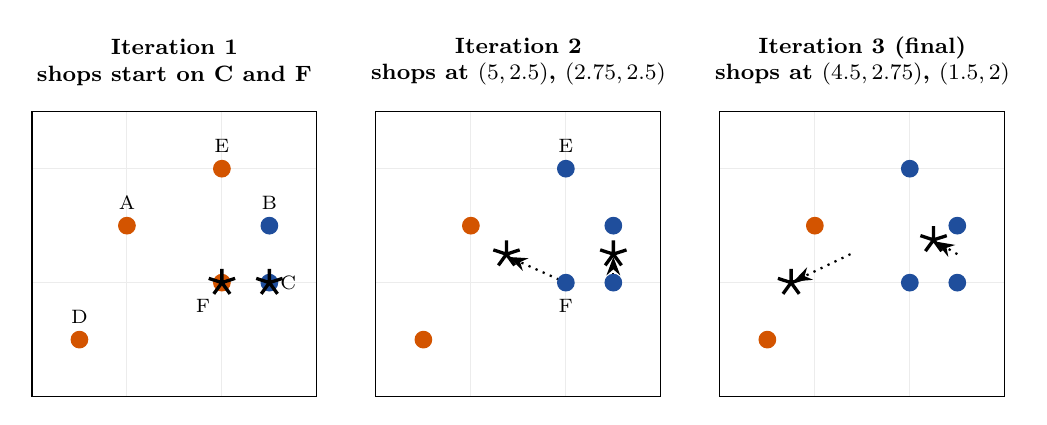
\begin{tikzpicture}
\begin{groupplot}[group style={group size=3 by 1,horizontal sep=0.75cm},width=5.2cm,height=5.2cm,
  xmin=0,xmax=6,ymin=0,ymax=5,ticks=none,grid=both,grid style={gray!15},title style={font=\footnotesize\bfseries,align=center}]
\nextgroupplot[title={Iteration 1\\shops start on C and F}]
\addplot[only marks,mark=*,mlblue,mark size=3pt] coordinates {(5,3)(5,2)};
\addplot[only marks,mark=*,mlorange,mark size=3pt] coordinates {(2,3)(1,1)(4,4)(4,2)};
\addplot[only marks,mark=star,black,mark size=5pt,very thick] coordinates {(5,2)(4,2)};
\node[font=\scriptsize] at (axis cs:2,3.4) {A}; \node[font=\scriptsize] at (axis cs:5,3.4) {B}; \node[font=\scriptsize] at (axis cs:5.4,2) {C};
\node[font=\scriptsize] at (axis cs:1,1.4) {D}; \node[font=\scriptsize] at (axis cs:4,4.4) {E}; \node[font=\scriptsize] at (axis cs:3.6,1.6) {F};
\nextgroupplot[title={Iteration 2\\shops at $(5,2.5)$, $(2.75,2.5)$}]
\addplot[only marks,mark=*,mlblue,mark size=3pt] coordinates {(5,3)(5,2)(4,4)(4,2)};
\addplot[only marks,mark=*,mlorange,mark size=3pt] coordinates {(2,3)(1,1)};
\addplot[only marks,mark=star,black,mark size=5pt,very thick] coordinates {(5,2.5)(2.75,2.5)};
\draw[-{Stealth},dotted,thick] (axis cs:5,2)--(axis cs:5,2.45);
\draw[-{Stealth},dotted,thick] (axis cs:4,2)--(axis cs:2.8,2.45);
\node[font=\scriptsize] at (axis cs:4,4.4) {E}; \node[font=\scriptsize] at (axis cs:4,1.6) {F};
\nextgroupplot[title={Iteration 3 (final)\\shops at $(4.5,2.75)$, $(1.5,2)$}]
\addplot[only marks,mark=*,mlblue,mark size=3pt] coordinates {(5,3)(5,2)(4,4)(4,2)};
\addplot[only marks,mark=*,mlorange,mark size=3pt] coordinates {(2,3)(1,1)};
\addplot[only marks,mark=star,black,mark size=5pt,very thick] coordinates {(4.5,2.75)(1.5,2)};
\draw[-{Stealth},dotted,thick] (axis cs:5,2.5)--(axis cs:4.55,2.72);
\draw[-{Stealth},dotted,thick] (axis cs:2.75,2.5)--(axis cs:1.55,2.02);
\end{groupplot}
\end{tikzpicture}
\caption{The K-Means run of the worked example. Stars are centroids; colours show the current cluster.}\label{fig:kmrun}
\end{figure}

\begin{explain}
Each panel is one iteration; the \textbf{stars} are the centroids and the \textbf{colours} show the cluster each point currently belongs to (blue = cluster~1, orange = cluster~2). In the first panel the two centroids start almost on top of each other, so the clustering is poor. In the second panel the dotted arrows show the centroids moving; points E and F have turned blue because they are now closer to the blue star. In the third panel the centroids have settled in the middle of their groups and nothing changes any more.
\end{explain}

\subsection{Initialisation and K-Means++}

Because K-Means only finds a local minimum, a bad start can give a bad result. If both initial shops land in the same neighbourhood, the final clusters can be poor.

\begin{definition}[: K-Means++ initialisation]
\textbf{K-Means++} chooses the first centroid uniformly at random from the data; each further centroid is chosen from the remaining points with probability \emph{proportional to $D(\vect x)^2$}, the squared distance from the point to the nearest centroid already chosen. This spreads the starting centroids far apart.
\end{definition}

\begin{example}[: K-Means++ probabilities]
One-dimensional points $0,\ 1,\ 10$; suppose the first centroid is $0$.
\[
  D^2=(0,\ 1,\ 100)\ \Rightarrow\ P=\Big(0,\ \tfrac1{101},\ \tfrac{100}{101}\Big)=(0,\ 0.0099,\ 0.990).
\]
The next centroid is almost certainly the far-away point $10$, giving well-separated starting centres.
\end{example}

\textbf{Real results.} We ran K-Means with $k=4$ on 300 points from four well-separated blobs, using a \emph{single} initialisation each time, 100 different random seeds:

\begin{center}
\begin{tabular}{@{}lccc@{}}
\toprule
\textbf{Initialisation} & \textbf{Mean inertia} & \textbf{Worst inertia} & \textbf{Runs reaching the best solution}\\
\midrule
Random points & 1513.6 & 6825.4 & 60 of 100\\
K-Means++ & 279.9 & 279.9 & \textbf{100 of 100}\\
\bottomrule
\end{tabular}
\end{center}

\noindent With random starts, 40\% of the runs got stuck in a bad local minimum (the worst had inertia 24 times larger!), while K-Means++ found the best solution every time. In practice we also run the algorithm several times (\texttt{n\_init=10}) and keep the run with the lowest inertia.

\subsection{Choosing the Number of Clusters $k$}

K-Means needs $k$ \emph{in advance}. Inertia always decreases as $k$ grows (with $k=n$ it is $0$), so we cannot simply minimise it. Two standard methods help.

\paragraph{1. The elbow method.} Run K-Means for $k=1,2,3,\dots$ and plot the inertia against $k$. Choose the $k$ at the ``elbow'', where adding more clusters stops giving a big improvement.

\paragraph{2. The silhouette score.}

\begin{definition}[: Silhouette coefficient]
For a point $i$ let $a(i)$ be the \textbf{average distance to the other points in its own cluster} (cohesion) and $b(i)$ the \textbf{smallest average distance to the points of any other cluster} (separation). Then
\[
  s(i)=\frac{b(i)-a(i)}{\max\{a(i),b(i)\}}\in[-1,1].
\]
$s\approx1$: the point is well inside its cluster; $s\approx0$: it lies on the border between two clusters; $s<0$: it is probably in the wrong cluster. The \textbf{silhouette score} of a clustering is the mean of $s(i)$ over all points; we choose the $k$ with the highest score.
\end{definition}

\begin{example}[: Silhouette by hand]
Four points on a line, clustered as $\{1,2\}$ and $\{8,9\}$.

\medskip
\textbf{Point 1:} $a=|1-2|=1$. $b=$ mean distance to $\{8,9\}=\frac{7+8}{2}=7.5$. $s=\frac{7.5-1}{7.5}=0.867$.\\
\textbf{Point 2:} $a=1$, $b=\frac{6+7}{2}=6.5$, $s=\frac{6.5-1}{6.5}=0.846$.\\
\textbf{Point 8:} $a=1$, $b=\frac{7+6}{2}=6.5$, $s=0.846$.\quad \textbf{Point 9:} $a=1$, $b=7.5$, $s=0.867$.

\medskip
Mean silhouette $=\frac{0.867+0.846+0.846+0.867}{4}=\mathbf{0.856}$: a very good clustering. If instead the clusters were $\{1,2,8\}$ and $\{9\}$, the point $8$ would have $a=\frac{7+6}2=6.5$ and $b=1$, so $s=\frac{1-6.5}{6.5}=-0.846<0$: a clearly wrong assignment.
\end{example}

\begin{figure}[!htbp]
\centering
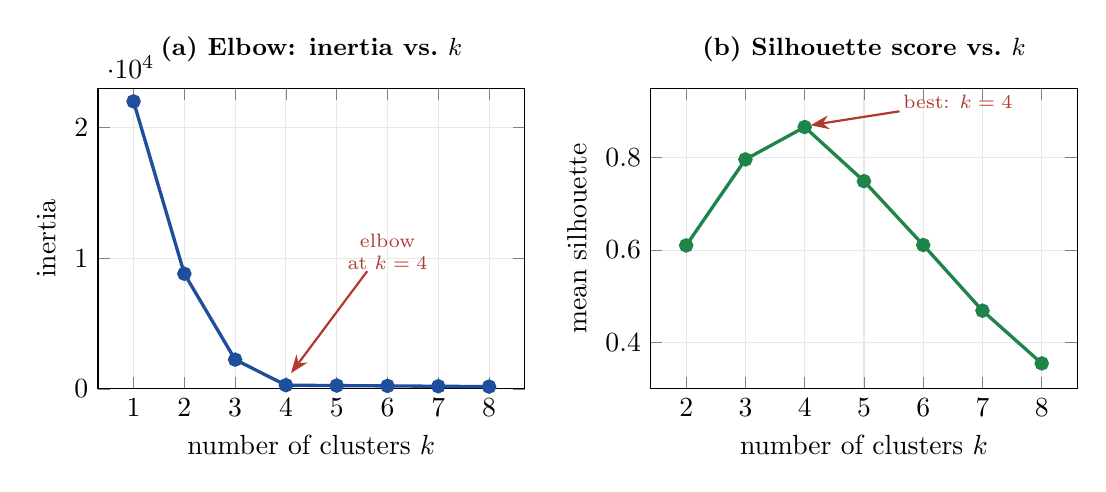
\begin{tikzpicture}
\begin{groupplot}[group style={group size=2 by 1,horizontal sep=1.6cm},width=7cm,height=5.4cm,grid=both,grid style={gray!18},
  title style={font=\small\bfseries},xlabel={number of clusters $k$},xtick={1,2,3,4,5,6,7,8}]
\nextgroupplot[title={(a) Elbow: inertia vs.\ $k$},ylabel={inertia},ymin=0,ymax=23000]
\addplot[very thick,mlblue,mark=*] coordinates {(1,21990.4)(2,8805.1)(3,2236.3)(4,279.9)(5,250.4)(6,223.3)(7,197.5)(8,171.1)};
\draw[mlred,thick,-{Stealth}] (axis cs:5.6,9000)--(axis cs:4.1,1200);
\node[font=\scriptsize,mlred,align=center] at (axis cs:6,10500) {elbow\\at $k=4$};
\nextgroupplot[title={(b) Silhouette score vs.\ $k$},ylabel={mean silhouette},ymin=0.3,ymax=0.95]
\addplot[very thick,mlgreen,mark=*] coordinates {(2,0.610)(3,0.796)(4,0.866)(5,0.749)(6,0.611)(7,0.469)(8,0.355)};
\draw[mlred,thick,-{Stealth}] (axis cs:5.6,0.9)--(axis cs:4.1,0.87);
\node[font=\scriptsize,mlred,anchor=west] at (axis cs:5.5,0.92) {best: $k=4$};
\end{groupplot}
\end{tikzpicture}
\caption{Choosing $k$ for 300 points drawn from 4 blobs (real K-Means results).}\label{fig:elbow}
\end{figure}

\begin{explain}
\textbf{(a) Elbow plot.} Going from 1 to 2 to 3 to 4 clusters the inertia collapses (21\,990 $\to$ 8\,805 $\to$ 2\,236 $\to$ 280). After $k=4$ it decreases only slowly (280 $\to$ 250 $\to$ 223 $\ldots$): extra clusters are just splitting blobs that were already compact. The \textbf{bend (elbow) at $k=4$} gives the answer, matching the four blobs that generated the data.

\medskip
\textbf{(b) Silhouette plot.} The score peaks at $k=4$ ($0.866$) and falls on both sides: with $k=3$ two blobs are forced together and with $k=5$ a blob is cut in two. The highest silhouette agrees with the elbow.
\end{explain}

\begin{warning}
The elbow is not always sharp, and for real data different methods may disagree. Use the elbow and silhouette as guidance together with \emph{domain knowledge} (for example, a company may only want 3 customer segments because it has 3 marketing teams).
\end{warning}

\begin{tryit}
\begin{lstlisting}
from sklearn.datasets import make_blobs
from sklearn.cluster import KMeans
from sklearn.metrics import silhouette_score

X, y = make_blobs(n_samples=300, centers=4, cluster_std=0.7,
                  random_state=7)

for k in range(2, 9):
    km = KMeans(n_clusters=k, init="k-means++", n_init=10,
                random_state=0).fit(X)
    print(k, round(km.inertia_, 1),
          round(silhouette_score(X, km.labels_), 3))
# k=4 -> inertia 279.9, silhouette 0.866 (best)
\end{lstlisting}
\emph{Challenge:} cluster the \textbf{iris} measurements with $k=3$ and compare the clusters with the true species using \texttt{adjusted\_rand\_score}.
\end{tryit}

\procon{K-Means}
{\item Simple, fast and easy to implement
 \item Scales to very large datasets (cost $O(nkd)$ per iteration)
 \item Always converges
 \item Gives centroids that summarise each group}
{\item Must choose $k$ in advance
 \item Result depends on initialisation (local minimum)
 \item Assumes round, similar-sized clusters
 \item Sensitive to outliers and feature scaling}
{\item Customer segmentation
 \item Image compression and segmentation
 \item Document and news grouping
 \item Vector quantisation, feature engineering}

%====================================================================
\section{Limits of K-Means}

K-Means is fast and popular, but it quietly assumes that clusters are \textbf{round blobs of similar size and density}. When this is not true, it fails. The main limits are:

\begin{enumerate}
  \item \textbf{$k$ must be chosen} before running the algorithm.
  \item \textbf{Local minima:} different starts can give different answers (reduce with K-Means++ and \texttt{n\_init}).
  \item \textbf{Cluster shape:} it uses distance to a centroid, so it can only produce convex, roughly spherical clusters. Moons, rings and elongated clusters are cut incorrectly.
  \item \textbf{Cluster size and density:} it tends to split a big cluster and merge small ones.
  \item \textbf{Outliers:} one extreme point drags a centroid away (the mean is not robust).
  \item \textbf{Feature scale:} features with a large range dominate the distance, so features must be standardised.
  \item \textbf{Hard assignments:} every point belongs to exactly one cluster, with no notion of uncertainty.
\end{enumerate}

\begin{example}[: The outlier problem]
One-dimensional data $\{1,2,3,100\}$ with a single cluster centre. The centroid is the mean
\[
  \mu=\frac{1+2+3+100}{4}=26.5,
\]
which is nowhere near the three points that actually form the group ($1,2,3$) and is not even close to the outlier. A single bad point has pulled the centre far away. (The \emph{median}, $2.5$, would have been unaffected: this is why K-Medians and K-Medoids exist.)
\end{example}

\begin{figure}[!htbp]
\centering
\begin{tikzpicture}
\begin{groupplot}[group style={group size=2 by 1,horizontal sep=1.2cm,group name=M},width=7.4cm,height=6cm,
  xmin=-1.5,xmax=2.5,ymin=-1,ymax=1.5,ticks=none,grid=both,grid style={gray!15},title style={font=\small\bfseries,align=center}]
\nextgroupplot[title={(a) K-Means with $k=2$\\ARI $=0.22$ (wrong)}]
\kmAplot
\kmBplot
\addplot[very thick,mlgreen,dashed,domain=-0.2:1.3]{0.229+2.291*(x-0.55)};
\addplot[only marks,mark=star,black,mark size=5pt,very thick] coordinates {(1.26,-0.08)(-0.16,0.54)};
\nextgroupplot[title={(b) DBSCAN ($\varepsilon=0.3$)\\ARI $=0.97$ (correct)}]
\dbAplot
\dbBplot
\dbNplot
\end{groupplot}
\pic[scale=1.1] at ([shift={(-0.7,-0.7)}]M c1r1.north east) {sad};
\pic[scale=1.1] at ([shift={(-0.7,-0.7)}]M c2r1.north east) {smile};
\end{tikzpicture}
\caption{Two interleaving half-moons (a 70-point sample): K-Means cuts them with a straight line, while DBSCAN follows their shape.}\label{fig:moons}
\end{figure}

\begin{explain}
The data are two half-moon shapes. \textbf{Panel (a):} K-Means looks for two round clusters. Its two centroids (stars) lie between the moons, and the cluster boundary is the \emph{straight green dashed line} halfway between them. This line slices \emph{through both moons}, so each cluster contains a piece of each moon: the \textbf{adjusted Rand index} (ARI, $1$ = perfect agreement with the true groups, $0$ = random) is only $0.22$. \textbf{Panel (b):} DBSCAN (Section~\ref{sec:dbscan}) follows the dense curved bands and recovers both moons exactly ($\text{ARI}=0.97$; the red cross is a point it declares noise).
\end{explain}

\begin{center}
\begin{tabular}{@{}lccc@{}}
\toprule
\textbf{Dataset (300 points)} & \textbf{K-Means} & \textbf{DBSCAN} & \textbf{Gaussian mixture}\\
\midrule
Round blobs & \textbf{1.00} & 0.93 (14 noise) & \textbf{1.00}\\
Unequal sizes and spreads & 0.99 & 0.91 (9 noise) & \textbf{1.00}\\
Stretched (elongated) blobs & 0.52 & 0.99 (2 noise) & \textbf{1.00}\\
Two moons & 0.23 & \textbf{1.00} & 0.46\\
Two concentric circles & $-0.00$ & \textbf{1.00} & $-0.00$\\
\bottomrule
\end{tabular}
\end{center}

\noindent \textit{Adjusted Rand index; real results; DBSCAN parameters were chosen per dataset ($\varepsilon=0.2$ for moons and circles, $0.5$--$0.7$ for blobs, 5 points minimum).} \textbf{Read the table:} on round blobs all methods succeed, but K-Means collapses on the elongated blobs ($0.52$), the moons ($0.23$) and the circles ($0.00$, no better than random). Gaussian mixtures cope with elongated clusters, and DBSCAN with arbitrary shapes. No single algorithm is best for every shape.

%====================================================================
\section{Using Clustering for Image Segmentation}\label{sec:seg}

\begin{definition}[: Image segmentation]
\textbf{Image segmentation} is the task of dividing an image into regions of pixels that belong together (for example sky, grass and a house). \textbf{Colour segmentation} with K-Means treats every pixel as a point $(R,G,B)$ in three-dimensional colour space, clusters the pixels into $k$ groups, and replaces every pixel by the \emph{centroid colour} of its cluster.
\end{definition}

\paragraph{Procedure.}
\begin{enumerate}
  \item Reshape the image of size $H\times W\times3$ into a list of $H\cdot W$ points with 3 features.
  \item Run K-Means with $k$ clusters (here $k$ = the number of colours wanted).
  \item Replace each pixel by the centroid of its cluster and reshape back to $H\times W\times3$.
\end{enumerate}

\begin{figure}[!htbp]
\centering
\resizebox{\linewidth}{!}{%
\begin{tikzpicture}[scale=0.62]
\node[font=\bfseries] at (2.6,4.4) {Original};
\node[font=\footnotesize] at (2.6,-0.6) {383 different colours};
\begin{scope}\fill[color={rgb,255:red,123;green,188;blue,238}] (0.00,3.30) rectangle ++(0.22,0.22);
\fill[color={rgb,255:red,107;green,189;blue,239}] (0.22,3.30) rectangle ++(0.22,0.22);
\fill[color={rgb,255:red,115;green,186;blue,239}] (0.44,3.30) rectangle ++(0.22,0.22);
\fill[color={rgb,255:red,123;green,180;blue,240}] (0.66,3.30) rectangle ++(0.22,0.22);
\fill[color={rgb,255:red,113;green,178;blue,230}] (0.88,3.30) rectangle ++(0.22,0.22);
\fill[color={rgb,255:red,126;green,180;blue,232}] (1.10,3.30) rectangle ++(0.22,0.22);
\fill[color={rgb,255:red,112;green,177;blue,235}] (1.32,3.30) rectangle ++(0.22,0.22);
\fill[color={rgb,255:red,117;green,193;blue,245}] (1.54,3.30) rectangle ++(0.22,0.22);
\fill[color={rgb,255:red,93;green,161;blue,233}] (1.76,3.30) rectangle ++(0.22,0.22);
\fill[color={rgb,255:red,116;green,182;blue,237}] (1.98,3.30) rectangle ++(0.22,0.22);
\fill[color={rgb,255:red,141;green,169;blue,231}] (2.20,3.30) rectangle ++(0.22,0.22);
\fill[color={rgb,255:red,140;green,186;blue,242}] (2.42,3.30) rectangle ++(0.22,0.22);
\fill[color={rgb,255:red,115;green,164;blue,237}] (2.64,3.30) rectangle ++(0.22,0.22);
\fill[color={rgb,255:red,121;green,168;blue,228}] (2.86,3.30) rectangle ++(0.22,0.22);
\fill[color={rgb,255:red,119;green,171;blue,234}] (3.08,3.30) rectangle ++(0.22,0.22);
\fill[color={rgb,255:red,121;green,180;blue,230}] (3.30,3.30) rectangle ++(0.22,0.22);
\fill[color={rgb,255:red,126;green,189;blue,238}] (3.52,3.30) rectangle ++(0.22,0.22);
\fill[color={rgb,255:red,112;green,187;blue,230}] (3.74,3.30) rectangle ++(0.22,0.22);
\fill[color={rgb,255:red,129;green,169;blue,244}] (3.96,3.30) rectangle ++(0.22,0.22);
\fill[color={rgb,255:red,120;green,168;blue,232}] (4.18,3.30) rectangle ++(0.22,0.22);
\fill[color={rgb,255:red,121;green,183;blue,225}] (4.40,3.30) rectangle ++(0.22,0.22);
\fill[color={rgb,255:red,109;green,182;blue,230}] (4.62,3.30) rectangle ++(0.22,0.22);
\fill[color={rgb,255:red,122;green,188;blue,219}] (4.84,3.30) rectangle ++(0.22,0.22);
\fill[color={rgb,255:red,123;green,192;blue,232}] (5.06,3.30) rectangle ++(0.22,0.22);
\fill[color={rgb,255:red,115;green,190;blue,236}] (0.00,3.08) rectangle ++(0.22,0.22);
\fill[color={rgb,255:red,132;green,179;blue,218}] (0.22,3.08) rectangle ++(0.22,0.22);
\fill[color={rgb,255:red,122;green,178;blue,241}] (0.44,3.08) rectangle ++(0.22,0.22);
\fill[color={rgb,255:red,125;green,166;blue,221}] (0.66,3.08) rectangle ++(0.22,0.22);
\fill[color={rgb,255:red,132;green,189;blue,227}] (0.88,3.08) rectangle ++(0.22,0.22);
\fill[color={rgb,255:red,123;green,186;blue,238}] (1.10,3.08) rectangle ++(0.22,0.22);
\fill[color={rgb,255:red,132;green,185;blue,232}] (1.32,3.08) rectangle ++(0.22,0.22);
\fill[color={rgb,255:red,120;green,193;blue,210}] (1.54,3.08) rectangle ++(0.22,0.22);
\fill[color={rgb,255:red,122;green,182;blue,219}] (1.76,3.08) rectangle ++(0.22,0.22);
\fill[color={rgb,255:red,126;green,175;blue,242}] (1.98,3.08) rectangle ++(0.22,0.22);
\fill[color={rgb,255:red,122;green,189;blue,245}] (2.20,3.08) rectangle ++(0.22,0.22);
\fill[color={rgb,255:red,127;green,173;blue,218}] (2.42,3.08) rectangle ++(0.22,0.22);
\fill[color={rgb,255:red,141;green,181;blue,226}] (2.64,3.08) rectangle ++(0.22,0.22);
\fill[color={rgb,255:red,124;green,180;blue,242}] (2.86,3.08) rectangle ++(0.22,0.22);
\fill[color={rgb,255:red,123;green,182;blue,226}] (3.08,3.08) rectangle ++(0.22,0.22);
\fill[color={rgb,255:red,128;green,172;blue,240}] (3.30,3.08) rectangle ++(0.22,0.22);
\fill[color={rgb,255:red,138;green,167;blue,208}] (3.52,3.08) rectangle ++(0.22,0.22);
\fill[color={rgb,255:red,129;green,207;blue,223}] (3.74,3.08) rectangle ++(0.22,0.22);
\fill[color={rgb,255:red,237;green,226;blue,52}] (3.96,3.08) rectangle ++(0.22,0.22);
\fill[color={rgb,255:red,245;green,217;blue,65}] (4.18,3.08) rectangle ++(0.22,0.22);
\fill[color={rgb,255:red,246;green,223;blue,58}] (4.40,3.08) rectangle ++(0.22,0.22);
\fill[color={rgb,255:red,115;green,179;blue,223}] (4.62,3.08) rectangle ++(0.22,0.22);
\fill[color={rgb,255:red,123;green,171;blue,222}] (4.84,3.08) rectangle ++(0.22,0.22);
\fill[color={rgb,255:red,138;green,181;blue,232}] (5.06,3.08) rectangle ++(0.22,0.22);
\fill[color={rgb,255:red,131;green,180;blue,229}] (0.00,2.86) rectangle ++(0.22,0.22);
\fill[color={rgb,255:red,130;green,187;blue,219}] (0.22,2.86) rectangle ++(0.22,0.22);
\fill[color={rgb,255:red,134;green,178;blue,220}] (0.44,2.86) rectangle ++(0.22,0.22);
\fill[color={rgb,255:red,117;green,180;blue,247}] (0.66,2.86) rectangle ++(0.22,0.22);
\fill[color={rgb,255:red,114;green,186;blue,210}] (0.88,2.86) rectangle ++(0.22,0.22);
\fill[color={rgb,255:red,126;green,193;blue,229}] (1.10,2.86) rectangle ++(0.22,0.22);
\fill[color={rgb,255:red,120;green,186;blue,238}] (1.32,2.86) rectangle ++(0.22,0.22);
\fill[color={rgb,255:red,133;green,204;blue,233}] (1.54,2.86) rectangle ++(0.22,0.22);
\fill[color={rgb,255:red,120;green,183;blue,230}] (1.76,2.86) rectangle ++(0.22,0.22);
\fill[color={rgb,255:red,127;green,184;blue,233}] (1.98,2.86) rectangle ++(0.22,0.22);
\fill[color={rgb,255:red,109;green,192;blue,225}] (2.20,2.86) rectangle ++(0.22,0.22);
\fill[color={rgb,255:red,114;green,190;blue,244}] (2.42,2.86) rectangle ++(0.22,0.22);
\fill[color={rgb,255:red,131;green,186;blue,222}] (2.64,2.86) rectangle ++(0.22,0.22);
\fill[color={rgb,255:red,155;green,193;blue,220}] (2.86,2.86) rectangle ++(0.22,0.22);
\fill[color={rgb,255:red,118;green,185;blue,215}] (3.08,2.86) rectangle ++(0.22,0.22);
\fill[color={rgb,255:red,128;green,179;blue,243}] (3.30,2.86) rectangle ++(0.22,0.22);
\fill[color={rgb,255:red,136;green,157;blue,231}] (3.52,2.86) rectangle ++(0.22,0.22);
\fill[color={rgb,255:red,234;green,231;blue,62}] (3.74,2.86) rectangle ++(0.22,0.22);
\fill[color={rgb,255:red,255;green,209;blue,78}] (3.96,2.86) rectangle ++(0.22,0.22);
\fill[color={rgb,255:red,255;green,209;blue,64}] (4.18,2.86) rectangle ++(0.22,0.22);
\fill[color={rgb,255:red,243;green,220;blue,47}] (4.40,2.86) rectangle ++(0.22,0.22);
\fill[color={rgb,255:red,255;green,210;blue,57}] (4.62,2.86) rectangle ++(0.22,0.22);
\fill[color={rgb,255:red,131;green,178;blue,229}] (4.84,2.86) rectangle ++(0.22,0.22);
\fill[color={rgb,255:red,120;green,183;blue,219}] (5.06,2.86) rectangle ++(0.22,0.22);
\fill[color={rgb,255:red,125;green,184;blue,226}] (0.00,2.64) rectangle ++(0.22,0.22);
\fill[color={rgb,255:red,130;green,183;blue,237}] (0.22,2.64) rectangle ++(0.22,0.22);
\fill[color={rgb,255:red,126;green,185;blue,222}] (0.44,2.64) rectangle ++(0.22,0.22);
\fill[color={rgb,255:red,124;green,173;blue,234}] (0.66,2.64) rectangle ++(0.22,0.22);
\fill[color={rgb,255:red,118;green,179;blue,233}] (0.88,2.64) rectangle ++(0.22,0.22);
\fill[color={rgb,255:red,133;green,182;blue,209}] (1.10,2.64) rectangle ++(0.22,0.22);
\fill[color={rgb,255:red,133;green,189;blue,215}] (1.32,2.64) rectangle ++(0.22,0.22);
\fill[color={rgb,255:red,137;green,179;blue,218}] (1.54,2.64) rectangle ++(0.22,0.22);
\fill[color={rgb,255:red,130;green,184;blue,231}] (1.76,2.64) rectangle ++(0.22,0.22);
\fill[color={rgb,255:red,113;green,204;blue,223}] (1.98,2.64) rectangle ++(0.22,0.22);
\fill[color={rgb,255:red,114;green,192;blue,225}] (2.20,2.64) rectangle ++(0.22,0.22);
\fill[color={rgb,255:red,132;green,183;blue,228}] (2.42,2.64) rectangle ++(0.22,0.22);
\fill[color={rgb,255:red,131;green,179;blue,236}] (2.64,2.64) rectangle ++(0.22,0.22);
\fill[color={rgb,255:red,124;green,177;blue,230}] (2.86,2.64) rectangle ++(0.22,0.22);
\fill[color={rgb,255:red,133;green,184;blue,220}] (3.08,2.64) rectangle ++(0.22,0.22);
\fill[color={rgb,255:red,135;green,168;blue,219}] (3.30,2.64) rectangle ++(0.22,0.22);
\fill[color={rgb,255:red,129;green,172;blue,229}] (3.52,2.64) rectangle ++(0.22,0.22);
\fill[color={rgb,255:red,249;green,229;blue,51}] (3.74,2.64) rectangle ++(0.22,0.22);
\fill[color={rgb,255:red,244;green,223;blue,35}] (3.96,2.64) rectangle ++(0.22,0.22);
\fill[color={rgb,255:red,255;green,213;blue,53}] (4.18,2.64) rectangle ++(0.22,0.22);
\fill[color={rgb,255:red,255;green,220;blue,42}] (4.40,2.64) rectangle ++(0.22,0.22);
\fill[color={rgb,255:red,255;green,229;blue,56}] (4.62,2.64) rectangle ++(0.22,0.22);
\fill[color={rgb,255:red,126;green,191;blue,220}] (4.84,2.64) rectangle ++(0.22,0.22);
\fill[color={rgb,255:red,133;green,188;blue,222}] (5.06,2.64) rectangle ++(0.22,0.22);
\fill[color={rgb,255:red,118;green,186;blue,218}] (0.00,2.42) rectangle ++(0.22,0.22);
\fill[color={rgb,255:red,142;green,189;blue,235}] (0.22,2.42) rectangle ++(0.22,0.22);
\fill[color={rgb,255:red,133;green,191;blue,219}] (0.44,2.42) rectangle ++(0.22,0.22);
\fill[color={rgb,255:red,139;green,206;blue,224}] (0.66,2.42) rectangle ++(0.22,0.22);
\fill[color={rgb,255:red,126;green,186;blue,222}] (0.88,2.42) rectangle ++(0.22,0.22);
\fill[color={rgb,255:red,125;green,189;blue,224}] (1.10,2.42) rectangle ++(0.22,0.22);
\fill[color={rgb,255:red,204;green,50;blue,53}] (1.32,2.42) rectangle ++(0.22,0.22);
\fill[color={rgb,255:red,200;green,47;blue,64}] (1.54,2.42) rectangle ++(0.22,0.22);
\fill[color={rgb,255:red,184;green,42;blue,46}] (1.76,2.42) rectangle ++(0.22,0.22);
\fill[color={rgb,255:red,189;green,36;blue,50}] (1.98,2.42) rectangle ++(0.22,0.22);
\fill[color={rgb,255:red,173;green,64;blue,49}] (2.20,2.42) rectangle ++(0.22,0.22);
\fill[color={rgb,255:red,184;green,41;blue,46}] (2.42,2.42) rectangle ++(0.22,0.22);
\fill[color={rgb,255:red,188;green,40;blue,41}] (2.64,2.42) rectangle ++(0.22,0.22);
\fill[color={rgb,255:red,188;green,45;blue,59}] (2.86,2.42) rectangle ++(0.22,0.22);
\fill[color={rgb,255:red,201;green,50;blue,55}] (3.08,2.42) rectangle ++(0.22,0.22);
\fill[color={rgb,255:red,119;green,194;blue,227}] (3.30,2.42) rectangle ++(0.22,0.22);
\fill[color={rgb,255:red,137;green,204;blue,204}] (3.52,2.42) rectangle ++(0.22,0.22);
\fill[color={rgb,255:red,253;green,209;blue,66}] (3.74,2.42) rectangle ++(0.22,0.22);
\fill[color={rgb,255:red,237;green,215;blue,62}] (3.96,2.42) rectangle ++(0.22,0.22);
\fill[color={rgb,255:red,255;green,221;blue,52}] (4.18,2.42) rectangle ++(0.22,0.22);
\fill[color={rgb,255:red,244;green,229;blue,60}] (4.40,2.42) rectangle ++(0.22,0.22);
\fill[color={rgb,255:red,233;green,228;blue,64}] (4.62,2.42) rectangle ++(0.22,0.22);
\fill[color={rgb,255:red,141;green,185;blue,235}] (4.84,2.42) rectangle ++(0.22,0.22);
\fill[color={rgb,255:red,121;green,194;blue,222}] (5.06,2.42) rectangle ++(0.22,0.22);
\fill[color={rgb,255:red,142;green,200;blue,218}] (0.00,2.20) rectangle ++(0.22,0.22);
\fill[color={rgb,255:red,134;green,190;blue,237}] (0.22,2.20) rectangle ++(0.22,0.22);
\fill[color={rgb,255:red,142;green,178;blue,230}] (0.44,2.20) rectangle ++(0.22,0.22);
\fill[color={rgb,255:red,142;green,211;blue,208}] (0.66,2.20) rectangle ++(0.22,0.22);
\fill[color={rgb,255:red,130;green,203;blue,211}] (0.88,2.20) rectangle ++(0.22,0.22);
\fill[color={rgb,255:red,123;green,195;blue,235}] (1.10,2.20) rectangle ++(0.22,0.22);
\fill[color={rgb,255:red,128;green,195;blue,226}] (1.32,2.20) rectangle ++(0.22,0.22);
\fill[color={rgb,255:red,185;green,100;blue,70}] (1.54,2.20) rectangle ++(0.22,0.22);
\fill[color={rgb,255:red,161;green,98;blue,59}] (1.76,2.20) rectangle ++(0.22,0.22);
\fill[color={rgb,255:red,181;green,106;blue,52}] (1.98,2.20) rectangle ++(0.22,0.22);
\fill[color={rgb,255:red,177;green,108;blue,59}] (2.20,2.20) rectangle ++(0.22,0.22);
\fill[color={rgb,255:red,167;green,98;blue,43}] (2.42,2.20) rectangle ++(0.22,0.22);
\fill[color={rgb,255:red,172;green,102;blue,51}] (2.64,2.20) rectangle ++(0.22,0.22);
\fill[color={rgb,255:red,177;green,86;blue,54}] (2.86,2.20) rectangle ++(0.22,0.22);
\fill[color={rgb,255:red,130;green,210;blue,209}] (3.08,2.20) rectangle ++(0.22,0.22);
\fill[color={rgb,255:red,141;green,199;blue,229}] (3.30,2.20) rectangle ++(0.22,0.22);
\fill[color={rgb,255:red,147;green,180;blue,202}] (3.52,2.20) rectangle ++(0.22,0.22);
\fill[color={rgb,255:red,143;green,178;blue,222}] (3.74,2.20) rectangle ++(0.22,0.22);
\fill[color={rgb,255:red,238;green,231;blue,69}] (3.96,2.20) rectangle ++(0.22,0.22);
\fill[color={rgb,255:red,243;green,229;blue,61}] (4.18,2.20) rectangle ++(0.22,0.22);
\fill[color={rgb,255:red,249;green,221;blue,58}] (4.40,2.20) rectangle ++(0.22,0.22);
\fill[color={rgb,255:red,141;green,193;blue,222}] (4.62,2.20) rectangle ++(0.22,0.22);
\fill[color={rgb,255:red,145;green,184;blue,228}] (4.84,2.20) rectangle ++(0.22,0.22);
\fill[color={rgb,255:red,139;green,205;blue,220}] (5.06,2.20) rectangle ++(0.22,0.22);
\fill[color={rgb,255:red,155;green,194;blue,221}] (0.00,1.98) rectangle ++(0.22,0.22);
\fill[color={rgb,255:red,131;green,198;blue,223}] (0.22,1.98) rectangle ++(0.22,0.22);
\fill[color={rgb,255:red,127;green,181;blue,217}] (0.44,1.98) rectangle ++(0.22,0.22);
\fill[color={rgb,255:red,131;green,203;blue,237}] (0.66,1.98) rectangle ++(0.22,0.22);
\fill[color={rgb,255:red,147;green,196;blue,219}] (0.88,1.98) rectangle ++(0.22,0.22);
\fill[color={rgb,255:red,139;green,201;blue,244}] (1.10,1.98) rectangle ++(0.22,0.22);
\fill[color={rgb,255:red,147;green,189;blue,223}] (1.32,1.98) rectangle ++(0.22,0.22);
\fill[color={rgb,255:red,165;green,92;blue,58}] (1.54,1.98) rectangle ++(0.22,0.22);
\fill[color={rgb,255:red,172;green,118;blue,61}] (1.76,1.98) rectangle ++(0.22,0.22);
\fill[color={rgb,255:red,184;green,118;blue,61}] (1.98,1.98) rectangle ++(0.22,0.22);
\fill[color={rgb,255:red,186;green,107;blue,56}] (2.20,1.98) rectangle ++(0.22,0.22);
\fill[color={rgb,255:red,173;green,100;blue,58}] (2.42,1.98) rectangle ++(0.22,0.22);
\fill[color={rgb,255:red,168;green,101;blue,64}] (2.64,1.98) rectangle ++(0.22,0.22);
\fill[color={rgb,255:red,161;green,100;blue,45}] (2.86,1.98) rectangle ++(0.22,0.22);
\fill[color={rgb,255:red,141;green,198;blue,225}] (3.08,1.98) rectangle ++(0.22,0.22);
\fill[color={rgb,255:red,141;green,198;blue,216}] (3.30,1.98) rectangle ++(0.22,0.22);
\fill[color={rgb,255:red,136;green,197;blue,233}] (3.52,1.98) rectangle ++(0.22,0.22);
\fill[color={rgb,255:red,142;green,218;blue,222}] (3.74,1.98) rectangle ++(0.22,0.22);
\fill[color={rgb,255:red,148;green,205;blue,222}] (3.96,1.98) rectangle ++(0.22,0.22);
\fill[color={rgb,255:red,130;green,180;blue,225}] (4.18,1.98) rectangle ++(0.22,0.22);
\fill[color={rgb,255:red,149;green,195;blue,225}] (4.40,1.98) rectangle ++(0.22,0.22);
\fill[color={rgb,255:red,134;green,198;blue,202}] (4.62,1.98) rectangle ++(0.22,0.22);
\fill[color={rgb,255:red,140;green,192;blue,209}] (4.84,1.98) rectangle ++(0.22,0.22);
\fill[color={rgb,255:red,160;green,178;blue,212}] (5.06,1.98) rectangle ++(0.22,0.22);
\fill[color={rgb,255:red,129;green,205;blue,212}] (0.00,1.76) rectangle ++(0.22,0.22);
\fill[color={rgb,255:red,148;green,200;blue,224}] (0.22,1.76) rectangle ++(0.22,0.22);
\fill[color={rgb,255:red,128;green,188;blue,238}] (0.44,1.76) rectangle ++(0.22,0.22);
\fill[color={rgb,255:red,128;green,186;blue,219}] (0.66,1.76) rectangle ++(0.22,0.22);
\fill[color={rgb,255:red,149;green,197;blue,228}] (0.88,1.76) rectangle ++(0.22,0.22);
\fill[color={rgb,255:red,130;green,203;blue,227}] (1.10,1.76) rectangle ++(0.22,0.22);
\fill[color={rgb,255:red,125;green,209;blue,244}] (1.32,1.76) rectangle ++(0.22,0.22);
\fill[color={rgb,255:red,162;green,101;blue,74}] (1.54,1.76) rectangle ++(0.22,0.22);
\fill[color={rgb,255:red,155;green,80;blue,47}] (1.76,1.76) rectangle ++(0.22,0.22);
\fill[color={rgb,255:red,164;green,94;blue,66}] (1.98,1.76) rectangle ++(0.22,0.22);
\fill[color={rgb,255:red,173;green,88;blue,66}] (2.20,1.76) rectangle ++(0.22,0.22);
\fill[color={rgb,255:red,189;green,112;blue,70}] (2.42,1.76) rectangle ++(0.22,0.22);
\fill[color={rgb,255:red,170;green,110;blue,50}] (2.64,1.76) rectangle ++(0.22,0.22);
\fill[color={rgb,255:red,178;green,99;blue,71}] (2.86,1.76) rectangle ++(0.22,0.22);
\fill[color={rgb,255:red,146;green,183;blue,222}] (3.08,1.76) rectangle ++(0.22,0.22);
\fill[color={rgb,255:red,153;green,183;blue,215}] (3.30,1.76) rectangle ++(0.22,0.22);
\fill[color={rgb,255:red,133;green,179;blue,231}] (3.52,1.76) rectangle ++(0.22,0.22);
\fill[color={rgb,255:red,154;green,202;blue,223}] (3.74,1.76) rectangle ++(0.22,0.22);
\fill[color={rgb,255:red,140;green,196;blue,214}] (3.96,1.76) rectangle ++(0.22,0.22);
\fill[color={rgb,255:red,150;green,204;blue,230}] (4.18,1.76) rectangle ++(0.22,0.22);
\fill[color={rgb,255:red,136;green,195;blue,219}] (4.40,1.76) rectangle ++(0.22,0.22);
\fill[color={rgb,255:red,159;green,196;blue,202}] (4.62,1.76) rectangle ++(0.22,0.22);
\fill[color={rgb,255:red,145;green,213;blue,228}] (4.84,1.76) rectangle ++(0.22,0.22);
\fill[color={rgb,255:red,150;green,194;blue,201}] (5.06,1.76) rectangle ++(0.22,0.22);
\fill[color={rgb,255:red,126;green,184;blue,218}] (0.00,1.54) rectangle ++(0.22,0.22);
\fill[color={rgb,255:red,147;green,203;blue,216}] (0.22,1.54) rectangle ++(0.22,0.22);
\fill[color={rgb,255:red,154;green,193;blue,212}] (0.44,1.54) rectangle ++(0.22,0.22);
\fill[color={rgb,255:red,153;green,187;blue,192}] (0.66,1.54) rectangle ++(0.22,0.22);
\fill[color={rgb,255:red,133;green,197;blue,188}] (0.88,1.54) rectangle ++(0.22,0.22);
\fill[color={rgb,255:red,140;green,193;blue,205}] (1.10,1.54) rectangle ++(0.22,0.22);
\fill[color={rgb,255:red,129;green,191;blue,214}] (1.32,1.54) rectangle ++(0.22,0.22);
\fill[color={rgb,255:red,183;green,104;blue,44}] (1.54,1.54) rectangle ++(0.22,0.22);
\fill[color={rgb,255:red,161;green,107;blue,79}] (1.76,1.54) rectangle ++(0.22,0.22);
\fill[color={rgb,255:red,94;green,63;blue,59}] (1.98,1.54) rectangle ++(0.22,0.22);
\fill[color={rgb,255:red,90;green,57;blue,26}] (2.20,1.54) rectangle ++(0.22,0.22);
\fill[color={rgb,255:red,165;green,122;blue,46}] (2.42,1.54) rectangle ++(0.22,0.22);
\fill[color={rgb,255:red,170;green,86;blue,61}] (2.64,1.54) rectangle ++(0.22,0.22);
\fill[color={rgb,255:red,179;green,98;blue,67}] (2.86,1.54) rectangle ++(0.22,0.22);
\fill[color={rgb,255:red,151;green,200;blue,236}] (3.08,1.54) rectangle ++(0.22,0.22);
\fill[color={rgb,255:red,152;green,193;blue,212}] (3.30,1.54) rectangle ++(0.22,0.22);
\fill[color={rgb,255:red,136;green,201;blue,216}] (3.52,1.54) rectangle ++(0.22,0.22);
\fill[color={rgb,255:red,171;green,214;blue,217}] (3.74,1.54) rectangle ++(0.22,0.22);
\fill[color={rgb,255:red,141;green,213;blue,200}] (3.96,1.54) rectangle ++(0.22,0.22);
\fill[color={rgb,255:red,139;green,206;blue,210}] (4.18,1.54) rectangle ++(0.22,0.22);
\fill[color={rgb,255:red,139;green,192;blue,226}] (4.40,1.54) rectangle ++(0.22,0.22);
\fill[color={rgb,255:red,145;green,200;blue,225}] (4.62,1.54) rectangle ++(0.22,0.22);
\fill[color={rgb,255:red,144;green,207;blue,212}] (4.84,1.54) rectangle ++(0.22,0.22);
\fill[color={rgb,255:red,130;green,178;blue,203}] (5.06,1.54) rectangle ++(0.22,0.22);
\fill[color={rgb,255:red,141;green,208;blue,219}] (0.00,1.32) rectangle ++(0.22,0.22);
\fill[color={rgb,255:red,141;green,187;blue,212}] (0.22,1.32) rectangle ++(0.22,0.22);
\fill[color={rgb,255:red,143;green,192;blue,203}] (0.44,1.32) rectangle ++(0.22,0.22);
\fill[color={rgb,255:red,142;green,208;blue,195}] (0.66,1.32) rectangle ++(0.22,0.22);
\fill[color={rgb,255:red,145;green,177;blue,219}] (0.88,1.32) rectangle ++(0.22,0.22);
\fill[color={rgb,255:red,140;green,177;blue,218}] (1.10,1.32) rectangle ++(0.22,0.22);
\fill[color={rgb,255:red,165;green,199;blue,229}] (1.32,1.32) rectangle ++(0.22,0.22);
\fill[color={rgb,255:red,169;green,78;blue,65}] (1.54,1.32) rectangle ++(0.22,0.22);
\fill[color={rgb,255:red,166;green,85;blue,68}] (1.76,1.32) rectangle ++(0.22,0.22);
\fill[color={rgb,255:red,93;green,55;blue,49}] (1.98,1.32) rectangle ++(0.22,0.22);
\fill[color={rgb,255:red,81;green,66;blue,31}] (2.20,1.32) rectangle ++(0.22,0.22);
\fill[color={rgb,255:red,175;green,89;blue,75}] (2.42,1.32) rectangle ++(0.22,0.22);
\fill[color={rgb,255:red,173;green,114;blue,52}] (2.64,1.32) rectangle ++(0.22,0.22);
\fill[color={rgb,255:red,165;green,108;blue,33}] (2.86,1.32) rectangle ++(0.22,0.22);
\fill[color={rgb,255:red,136;green,208;blue,222}] (3.08,1.32) rectangle ++(0.22,0.22);
\fill[color={rgb,255:red,157;green,195;blue,223}] (3.30,1.32) rectangle ++(0.22,0.22);
\fill[color={rgb,255:red,140;green,184;blue,200}] (3.52,1.32) rectangle ++(0.22,0.22);
\fill[color={rgb,255:red,141;green,193;blue,211}] (3.74,1.32) rectangle ++(0.22,0.22);
\fill[color={rgb,255:red,112;green,178;blue,212}] (3.96,1.32) rectangle ++(0.22,0.22);
\fill[color={rgb,255:red,150;green,192;blue,208}] (4.18,1.32) rectangle ++(0.22,0.22);
\fill[color={rgb,255:red,124;green,218;blue,206}] (4.40,1.32) rectangle ++(0.22,0.22);
\fill[color={rgb,255:red,164;green,214;blue,220}] (4.62,1.32) rectangle ++(0.22,0.22);
\fill[color={rgb,255:red,141;green,199;blue,205}] (4.84,1.32) rectangle ++(0.22,0.22);
\fill[color={rgb,255:red,150;green,198;blue,222}] (5.06,1.32) rectangle ++(0.22,0.22);
\fill[color={rgb,255:red,70;green,167;blue,56}] (0.00,1.10) rectangle ++(0.22,0.22);
\fill[color={rgb,255:red,70;green,142;blue,51}] (0.22,1.10) rectangle ++(0.22,0.22);
\fill[color={rgb,255:red,54;green,140;blue,70}] (0.44,1.10) rectangle ++(0.22,0.22);
\fill[color={rgb,255:red,69;green,163;blue,60}] (0.66,1.10) rectangle ++(0.22,0.22);
\fill[color={rgb,255:red,63;green,144;blue,48}] (0.88,1.10) rectangle ++(0.22,0.22);
\fill[color={rgb,255:red,64;green,153;blue,49}] (1.10,1.10) rectangle ++(0.22,0.22);
\fill[color={rgb,255:red,66;green,133;blue,58}] (1.32,1.10) rectangle ++(0.22,0.22);
\fill[color={rgb,255:red,164;green,95;blue,49}] (1.54,1.10) rectangle ++(0.22,0.22);
\fill[color={rgb,255:red,180;green,106;blue,72}] (1.76,1.10) rectangle ++(0.22,0.22);
\fill[color={rgb,255:red,91;green,47;blue,36}] (1.98,1.10) rectangle ++(0.22,0.22);
\fill[color={rgb,255:red,78;green,64;blue,52}] (2.20,1.10) rectangle ++(0.22,0.22);
\fill[color={rgb,255:red,173;green,94;blue,56}] (2.42,1.10) rectangle ++(0.22,0.22);
\fill[color={rgb,255:red,172;green,85;blue,61}] (2.64,1.10) rectangle ++(0.22,0.22);
\fill[color={rgb,255:red,172;green,94;blue,56}] (2.86,1.10) rectangle ++(0.22,0.22);
\fill[color={rgb,255:red,62;green,142;blue,52}] (3.08,1.10) rectangle ++(0.22,0.22);
\fill[color={rgb,255:red,68;green,152;blue,77}] (3.30,1.10) rectangle ++(0.22,0.22);
\fill[color={rgb,255:red,50;green,132;blue,69}] (3.52,1.10) rectangle ++(0.22,0.22);
\fill[color={rgb,255:red,69;green,142;blue,45}] (3.74,1.10) rectangle ++(0.22,0.22);
\fill[color={rgb,255:red,59;green,132;blue,56}] (3.96,1.10) rectangle ++(0.22,0.22);
\fill[color={rgb,255:red,38;green,147;blue,38}] (4.18,1.10) rectangle ++(0.22,0.22);
\fill[color={rgb,255:red,57;green,165;blue,57}] (4.40,1.10) rectangle ++(0.22,0.22);
\fill[color={rgb,255:red,67;green,143;blue,51}] (4.62,1.10) rectangle ++(0.22,0.22);
\fill[color={rgb,255:red,45;green,160;blue,59}] (4.84,1.10) rectangle ++(0.22,0.22);
\fill[color={rgb,255:red,76;green,138;blue,57}] (5.06,1.10) rectangle ++(0.22,0.22);
\fill[color={rgb,255:red,60;green,164;blue,78}] (0.00,0.88) rectangle ++(0.22,0.22);
\fill[color={rgb,255:red,53;green,138;blue,42}] (0.22,0.88) rectangle ++(0.22,0.22);
\fill[color={rgb,255:red,73;green,149;blue,53}] (0.44,0.88) rectangle ++(0.22,0.22);
\fill[color={rgb,255:red,59;green,124;blue,42}] (0.66,0.88) rectangle ++(0.22,0.22);
\fill[color={rgb,255:red,69;green,153;blue,61}] (0.88,0.88) rectangle ++(0.22,0.22);
\fill[color={rgb,255:red,49;green,155;blue,77}] (1.10,0.88) rectangle ++(0.22,0.22);
\fill[color={rgb,255:red,47;green,150;blue,55}] (1.32,0.88) rectangle ++(0.22,0.22);
\fill[color={rgb,255:red,173;green,100;blue,58}] (1.54,0.88) rectangle ++(0.22,0.22);
\fill[color={rgb,255:red,161;green,99;blue,53}] (1.76,0.88) rectangle ++(0.22,0.22);
\fill[color={rgb,255:red,88;green,59;blue,46}] (1.98,0.88) rectangle ++(0.22,0.22);
\fill[color={rgb,255:red,84;green,56;blue,50}] (2.20,0.88) rectangle ++(0.22,0.22);
\fill[color={rgb,255:red,167;green,97;blue,68}] (2.42,0.88) rectangle ++(0.22,0.22);
\fill[color={rgb,255:red,172;green,100;blue,62}] (2.64,0.88) rectangle ++(0.22,0.22);
\fill[color={rgb,255:red,157;green,104;blue,73}] (2.86,0.88) rectangle ++(0.22,0.22);
\fill[color={rgb,255:red,65;green,134;blue,62}] (3.08,0.88) rectangle ++(0.22,0.22);
\fill[color={rgb,255:red,50;green,147;blue,61}] (3.30,0.88) rectangle ++(0.22,0.22);
\fill[color={rgb,255:red,48;green,163;blue,59}] (3.52,0.88) rectangle ++(0.22,0.22);
\fill[color={rgb,255:red,68;green,156;blue,73}] (3.74,0.88) rectangle ++(0.22,0.22);
\fill[color={rgb,255:red,72;green,135;blue,60}] (3.96,0.88) rectangle ++(0.22,0.22);
\fill[color={rgb,255:red,38;green,145;blue,67}] (4.18,0.88) rectangle ++(0.22,0.22);
\fill[color={rgb,255:red,69;green,163;blue,56}] (4.40,0.88) rectangle ++(0.22,0.22);
\fill[color={rgb,255:red,63;green,151;blue,72}] (4.62,0.88) rectangle ++(0.22,0.22);
\fill[color={rgb,255:red,76;green,146;blue,98}] (4.84,0.88) rectangle ++(0.22,0.22);
\fill[color={rgb,255:red,60;green,146;blue,66}] (5.06,0.88) rectangle ++(0.22,0.22);
\fill[color={rgb,255:red,67;green,155;blue,53}] (0.00,0.66) rectangle ++(0.22,0.22);
\fill[color={rgb,255:red,74;green,150;blue,75}] (0.22,0.66) rectangle ++(0.22,0.22);
\fill[color={rgb,255:red,74;green,137;blue,50}] (0.44,0.66) rectangle ++(0.22,0.22);
\fill[color={rgb,255:red,50;green,152;blue,60}] (0.66,0.66) rectangle ++(0.22,0.22);
\fill[color={rgb,255:red,62;green,142;blue,64}] (0.88,0.66) rectangle ++(0.22,0.22);
\fill[color={rgb,255:red,74;green,136;blue,58}] (1.10,0.66) rectangle ++(0.22,0.22);
\fill[color={rgb,255:red,62;green,149;blue,58}] (1.32,0.66) rectangle ++(0.22,0.22);
\fill[color={rgb,255:red,78;green,163;blue,68}] (1.54,0.66) rectangle ++(0.22,0.22);
\fill[color={rgb,255:red,52;green,172;blue,63}] (1.76,0.66) rectangle ++(0.22,0.22);
\fill[color={rgb,255:red,54;green,146;blue,55}] (1.98,0.66) rectangle ++(0.22,0.22);
\fill[color={rgb,255:red,81;green,152;blue,60}] (2.20,0.66) rectangle ++(0.22,0.22);
\fill[color={rgb,255:red,38;green,157;blue,49}] (2.42,0.66) rectangle ++(0.22,0.22);
\fill[color={rgb,255:red,49;green,156;blue,51}] (2.64,0.66) rectangle ++(0.22,0.22);
\fill[color={rgb,255:red,68;green,161;blue,42}] (2.86,0.66) rectangle ++(0.22,0.22);
\fill[color={rgb,255:red,59;green,134;blue,59}] (3.08,0.66) rectangle ++(0.22,0.22);
\fill[color={rgb,255:red,69;green,136;blue,78}] (3.30,0.66) rectangle ++(0.22,0.22);
\fill[color={rgb,255:red,57;green,138;blue,59}] (3.52,0.66) rectangle ++(0.22,0.22);
\fill[color={rgb,255:red,68;green,136;blue,60}] (3.74,0.66) rectangle ++(0.22,0.22);
\fill[color={rgb,255:red,46;green,162;blue,61}] (3.96,0.66) rectangle ++(0.22,0.22);
\fill[color={rgb,255:red,56;green,160;blue,47}] (4.18,0.66) rectangle ++(0.22,0.22);
\fill[color={rgb,255:red,56;green,168;blue,59}] (4.40,0.66) rectangle ++(0.22,0.22);
\fill[color={rgb,255:red,73;green,152;blue,53}] (4.62,0.66) rectangle ++(0.22,0.22);
\fill[color={rgb,255:red,57;green,151;blue,56}] (4.84,0.66) rectangle ++(0.22,0.22);
\fill[color={rgb,255:red,52;green,142;blue,45}] (5.06,0.66) rectangle ++(0.22,0.22);
\fill[color={rgb,255:red,61;green,154;blue,67}] (0.00,0.44) rectangle ++(0.22,0.22);
\fill[color={rgb,255:red,42;green,158;blue,60}] (0.22,0.44) rectangle ++(0.22,0.22);
\fill[color={rgb,255:red,45;green,151;blue,68}] (0.44,0.44) rectangle ++(0.22,0.22);
\fill[color={rgb,255:red,65;green,157;blue,69}] (0.66,0.44) rectangle ++(0.22,0.22);
\fill[color={rgb,255:red,69;green,149;blue,39}] (0.88,0.44) rectangle ++(0.22,0.22);
\fill[color={rgb,255:red,52;green,153;blue,55}] (1.10,0.44) rectangle ++(0.22,0.22);
\fill[color={rgb,255:red,67;green,158;blue,60}] (1.32,0.44) rectangle ++(0.22,0.22);
\fill[color={rgb,255:red,79;green,140;blue,69}] (1.54,0.44) rectangle ++(0.22,0.22);
\fill[color={rgb,255:red,55;green,142;blue,66}] (1.76,0.44) rectangle ++(0.22,0.22);
\fill[color={rgb,255:red,54;green,158;blue,48}] (1.98,0.44) rectangle ++(0.22,0.22);
\fill[color={rgb,255:red,60;green,141;blue,57}] (2.20,0.44) rectangle ++(0.22,0.22);
\fill[color={rgb,255:red,56;green,139;blue,66}] (2.42,0.44) rectangle ++(0.22,0.22);
\fill[color={rgb,255:red,47;green,140;blue,69}] (2.64,0.44) rectangle ++(0.22,0.22);
\fill[color={rgb,255:red,70;green,156;blue,63}] (2.86,0.44) rectangle ++(0.22,0.22);
\fill[color={rgb,255:red,83;green,138;blue,52}] (3.08,0.44) rectangle ++(0.22,0.22);
\fill[color={rgb,255:red,50;green,159;blue,63}] (3.30,0.44) rectangle ++(0.22,0.22);
\fill[color={rgb,255:red,71;green,160;blue,58}] (3.52,0.44) rectangle ++(0.22,0.22);
\fill[color={rgb,255:red,52;green,140;blue,82}] (3.74,0.44) rectangle ++(0.22,0.22);
\fill[color={rgb,255:red,70;green,156;blue,56}] (3.96,0.44) rectangle ++(0.22,0.22);
\fill[color={rgb,255:red,58;green,146;blue,57}] (4.18,0.44) rectangle ++(0.22,0.22);
\fill[color={rgb,255:red,36;green,149;blue,56}] (4.40,0.44) rectangle ++(0.22,0.22);
\fill[color={rgb,255:red,63;green,152;blue,68}] (4.62,0.44) rectangle ++(0.22,0.22);
\fill[color={rgb,255:red,60;green,158;blue,34}] (4.84,0.44) rectangle ++(0.22,0.22);
\fill[color={rgb,255:red,49;green,167;blue,48}] (5.06,0.44) rectangle ++(0.22,0.22);
\fill[color={rgb,255:red,57;green,157;blue,51}] (0.00,0.22) rectangle ++(0.22,0.22);
\fill[color={rgb,255:red,67;green,136;blue,41}] (0.22,0.22) rectangle ++(0.22,0.22);
\fill[color={rgb,255:red,47;green,133;blue,60}] (0.44,0.22) rectangle ++(0.22,0.22);
\fill[color={rgb,255:red,57;green,153;blue,50}] (0.66,0.22) rectangle ++(0.22,0.22);
\fill[color={rgb,255:red,85;green,149;blue,59}] (0.88,0.22) rectangle ++(0.22,0.22);
\fill[color={rgb,255:red,64;green,147;blue,54}] (1.10,0.22) rectangle ++(0.22,0.22);
\fill[color={rgb,255:red,61;green,159;blue,67}] (1.32,0.22) rectangle ++(0.22,0.22);
\fill[color={rgb,255:red,69;green,144;blue,52}] (1.54,0.22) rectangle ++(0.22,0.22);
\fill[color={rgb,255:red,80;green,147;blue,65}] (1.76,0.22) rectangle ++(0.22,0.22);
\fill[color={rgb,255:red,67;green,164;blue,46}] (1.98,0.22) rectangle ++(0.22,0.22);
\fill[color={rgb,255:red,55;green,146;blue,57}] (2.20,0.22) rectangle ++(0.22,0.22);
\fill[color={rgb,255:red,36;green,149;blue,31}] (2.42,0.22) rectangle ++(0.22,0.22);
\fill[color={rgb,255:red,63;green,155;blue,66}] (2.64,0.22) rectangle ++(0.22,0.22);
\fill[color={rgb,255:red,48;green,159;blue,51}] (2.86,0.22) rectangle ++(0.22,0.22);
\fill[color={rgb,255:red,48;green,140;blue,51}] (3.08,0.22) rectangle ++(0.22,0.22);
\fill[color={rgb,255:red,62;green,158;blue,39}] (3.30,0.22) rectangle ++(0.22,0.22);
\fill[color={rgb,255:red,55;green,159;blue,62}] (3.52,0.22) rectangle ++(0.22,0.22);
\fill[color={rgb,255:red,65;green,135;blue,69}] (3.74,0.22) rectangle ++(0.22,0.22);
\fill[color={rgb,255:red,44;green,152;blue,74}] (3.96,0.22) rectangle ++(0.22,0.22);
\fill[color={rgb,255:red,79;green,155;blue,69}] (4.18,0.22) rectangle ++(0.22,0.22);
\fill[color={rgb,255:red,54;green,145;blue,72}] (4.40,0.22) rectangle ++(0.22,0.22);
\fill[color={rgb,255:red,60;green,149;blue,46}] (4.62,0.22) rectangle ++(0.22,0.22);
\fill[color={rgb,255:red,62;green,156;blue,52}] (4.84,0.22) rectangle ++(0.22,0.22);
\fill[color={rgb,255:red,55;green,166;blue,62}] (5.06,0.22) rectangle ++(0.22,0.22);
\fill[color={rgb,255:red,57;green,139;blue,54}] (0.00,0.00) rectangle ++(0.22,0.22);
\fill[color={rgb,255:red,58;green,164;blue,54}] (0.22,0.00) rectangle ++(0.22,0.22);
\fill[color={rgb,255:red,78;green,141;blue,56}] (0.44,0.00) rectangle ++(0.22,0.22);
\fill[color={rgb,255:red,68;green,148;blue,52}] (0.66,0.00) rectangle ++(0.22,0.22);
\fill[color={rgb,255:red,59;green,154;blue,43}] (0.88,0.00) rectangle ++(0.22,0.22);
\fill[color={rgb,255:red,58;green,149;blue,56}] (1.10,0.00) rectangle ++(0.22,0.22);
\fill[color={rgb,255:red,67;green,144;blue,56}] (1.32,0.00) rectangle ++(0.22,0.22);
\fill[color={rgb,255:red,60;green,157;blue,58}] (1.54,0.00) rectangle ++(0.22,0.22);
\fill[color={rgb,255:red,75;green,141;blue,73}] (1.76,0.00) rectangle ++(0.22,0.22);
\fill[color={rgb,255:red,51;green,148;blue,64}] (1.98,0.00) rectangle ++(0.22,0.22);
\fill[color={rgb,255:red,81;green,159;blue,56}] (2.20,0.00) rectangle ++(0.22,0.22);
\fill[color={rgb,255:red,73;green,148;blue,52}] (2.42,0.00) rectangle ++(0.22,0.22);
\fill[color={rgb,255:red,64;green,151;blue,70}] (2.64,0.00) rectangle ++(0.22,0.22);
\fill[color={rgb,255:red,55;green,154;blue,66}] (2.86,0.00) rectangle ++(0.22,0.22);
\fill[color={rgb,255:red,63;green,150;blue,53}] (3.08,0.00) rectangle ++(0.22,0.22);
\fill[color={rgb,255:red,69;green,151;blue,65}] (3.30,0.00) rectangle ++(0.22,0.22);
\fill[color={rgb,255:red,56;green,150;blue,50}] (3.52,0.00) rectangle ++(0.22,0.22);
\fill[color={rgb,255:red,61;green,158;blue,61}] (3.74,0.00) rectangle ++(0.22,0.22);
\fill[color={rgb,255:red,69;green,153;blue,74}] (3.96,0.00) rectangle ++(0.22,0.22);
\fill[color={rgb,255:red,58;green,134;blue,64}] (4.18,0.00) rectangle ++(0.22,0.22);
\fill[color={rgb,255:red,58;green,140;blue,67}] (4.40,0.00) rectangle ++(0.22,0.22);
\fill[color={rgb,255:red,63;green,154;blue,57}] (4.62,0.00) rectangle ++(0.22,0.22);
\fill[color={rgb,255:red,62;green,153;blue,78}] (4.84,0.00) rectangle ++(0.22,0.22);
\fill[color={rgb,255:red,53;green,150;blue,64}] (5.06,0.00) rectangle ++(0.22,0.22);
\end{scope}
\draw[-{Stealth},very thick,mlpurple] (5.8,1.8)--(7.2,1.8);
\begin{scope}[xshift=7.6cm]
\node[font=\bfseries] at (2.6,4.4) {$k=2$ colours};
\node[font=\footnotesize] at (2.6,-0.6) {inertia $1.41\times10^{6}$};
\fill[color={rgb,255:red,133;green,189;blue,224}] (0.00,3.30) rectangle ++(0.22,0.22);
\fill[color={rgb,255:red,133;green,189;blue,224}] (0.22,3.30) rectangle ++(0.22,0.22);
\fill[color={rgb,255:red,133;green,189;blue,224}] (0.44,3.30) rectangle ++(0.22,0.22);
\fill[color={rgb,255:red,133;green,189;blue,224}] (0.66,3.30) rectangle ++(0.22,0.22);
\fill[color={rgb,255:red,133;green,189;blue,224}] (0.88,3.30) rectangle ++(0.22,0.22);
\fill[color={rgb,255:red,133;green,189;blue,224}] (1.10,3.30) rectangle ++(0.22,0.22);
\fill[color={rgb,255:red,133;green,189;blue,224}] (1.32,3.30) rectangle ++(0.22,0.22);
\fill[color={rgb,255:red,133;green,189;blue,224}] (1.54,3.30) rectangle ++(0.22,0.22);
\fill[color={rgb,255:red,133;green,189;blue,224}] (1.76,3.30) rectangle ++(0.22,0.22);
\fill[color={rgb,255:red,133;green,189;blue,224}] (1.98,3.30) rectangle ++(0.22,0.22);
\fill[color={rgb,255:red,133;green,189;blue,224}] (2.20,3.30) rectangle ++(0.22,0.22);
\fill[color={rgb,255:red,133;green,189;blue,224}] (2.42,3.30) rectangle ++(0.22,0.22);
\fill[color={rgb,255:red,133;green,189;blue,224}] (2.64,3.30) rectangle ++(0.22,0.22);
\fill[color={rgb,255:red,133;green,189;blue,224}] (2.86,3.30) rectangle ++(0.22,0.22);
\fill[color={rgb,255:red,133;green,189;blue,224}] (3.08,3.30) rectangle ++(0.22,0.22);
\fill[color={rgb,255:red,133;green,189;blue,224}] (3.30,3.30) rectangle ++(0.22,0.22);
\fill[color={rgb,255:red,133;green,189;blue,224}] (3.52,3.30) rectangle ++(0.22,0.22);
\fill[color={rgb,255:red,133;green,189;blue,224}] (3.74,3.30) rectangle ++(0.22,0.22);
\fill[color={rgb,255:red,133;green,189;blue,224}] (3.96,3.30) rectangle ++(0.22,0.22);
\fill[color={rgb,255:red,133;green,189;blue,224}] (4.18,3.30) rectangle ++(0.22,0.22);
\fill[color={rgb,255:red,133;green,189;blue,224}] (4.40,3.30) rectangle ++(0.22,0.22);
\fill[color={rgb,255:red,133;green,189;blue,224}] (4.62,3.30) rectangle ++(0.22,0.22);
\fill[color={rgb,255:red,133;green,189;blue,224}] (4.84,3.30) rectangle ++(0.22,0.22);
\fill[color={rgb,255:red,133;green,189;blue,224}] (5.06,3.30) rectangle ++(0.22,0.22);
\fill[color={rgb,255:red,133;green,189;blue,224}] (0.00,3.08) rectangle ++(0.22,0.22);
\fill[color={rgb,255:red,133;green,189;blue,224}] (0.22,3.08) rectangle ++(0.22,0.22);
\fill[color={rgb,255:red,133;green,189;blue,224}] (0.44,3.08) rectangle ++(0.22,0.22);
\fill[color={rgb,255:red,133;green,189;blue,224}] (0.66,3.08) rectangle ++(0.22,0.22);
\fill[color={rgb,255:red,133;green,189;blue,224}] (0.88,3.08) rectangle ++(0.22,0.22);
\fill[color={rgb,255:red,133;green,189;blue,224}] (1.10,3.08) rectangle ++(0.22,0.22);
\fill[color={rgb,255:red,133;green,189;blue,224}] (1.32,3.08) rectangle ++(0.22,0.22);
\fill[color={rgb,255:red,133;green,189;blue,224}] (1.54,3.08) rectangle ++(0.22,0.22);
\fill[color={rgb,255:red,133;green,189;blue,224}] (1.76,3.08) rectangle ++(0.22,0.22);
\fill[color={rgb,255:red,133;green,189;blue,224}] (1.98,3.08) rectangle ++(0.22,0.22);
\fill[color={rgb,255:red,133;green,189;blue,224}] (2.20,3.08) rectangle ++(0.22,0.22);
\fill[color={rgb,255:red,133;green,189;blue,224}] (2.42,3.08) rectangle ++(0.22,0.22);
\fill[color={rgb,255:red,133;green,189;blue,224}] (2.64,3.08) rectangle ++(0.22,0.22);
\fill[color={rgb,255:red,133;green,189;blue,224}] (2.86,3.08) rectangle ++(0.22,0.22);
\fill[color={rgb,255:red,133;green,189;blue,224}] (3.08,3.08) rectangle ++(0.22,0.22);
\fill[color={rgb,255:red,133;green,189;blue,224}] (3.30,3.08) rectangle ++(0.22,0.22);
\fill[color={rgb,255:red,133;green,189;blue,224}] (3.52,3.08) rectangle ++(0.22,0.22);
\fill[color={rgb,255:red,133;green,189;blue,224}] (3.74,3.08) rectangle ++(0.22,0.22);
\fill[color={rgb,255:red,108;green,139;blue,58}] (3.96,3.08) rectangle ++(0.22,0.22);
\fill[color={rgb,255:red,108;green,139;blue,58}] (4.18,3.08) rectangle ++(0.22,0.22);
\fill[color={rgb,255:red,108;green,139;blue,58}] (4.40,3.08) rectangle ++(0.22,0.22);
\fill[color={rgb,255:red,133;green,189;blue,224}] (4.62,3.08) rectangle ++(0.22,0.22);
\fill[color={rgb,255:red,133;green,189;blue,224}] (4.84,3.08) rectangle ++(0.22,0.22);
\fill[color={rgb,255:red,133;green,189;blue,224}] (5.06,3.08) rectangle ++(0.22,0.22);
\fill[color={rgb,255:red,133;green,189;blue,224}] (0.00,2.86) rectangle ++(0.22,0.22);
\fill[color={rgb,255:red,133;green,189;blue,224}] (0.22,2.86) rectangle ++(0.22,0.22);
\fill[color={rgb,255:red,133;green,189;blue,224}] (0.44,2.86) rectangle ++(0.22,0.22);
\fill[color={rgb,255:red,133;green,189;blue,224}] (0.66,2.86) rectangle ++(0.22,0.22);
\fill[color={rgb,255:red,133;green,189;blue,224}] (0.88,2.86) rectangle ++(0.22,0.22);
\fill[color={rgb,255:red,133;green,189;blue,224}] (1.10,2.86) rectangle ++(0.22,0.22);
\fill[color={rgb,255:red,133;green,189;blue,224}] (1.32,2.86) rectangle ++(0.22,0.22);
\fill[color={rgb,255:red,133;green,189;blue,224}] (1.54,2.86) rectangle ++(0.22,0.22);
\fill[color={rgb,255:red,133;green,189;blue,224}] (1.76,2.86) rectangle ++(0.22,0.22);
\fill[color={rgb,255:red,133;green,189;blue,224}] (1.98,2.86) rectangle ++(0.22,0.22);
\fill[color={rgb,255:red,133;green,189;blue,224}] (2.20,2.86) rectangle ++(0.22,0.22);
\fill[color={rgb,255:red,133;green,189;blue,224}] (2.42,2.86) rectangle ++(0.22,0.22);
\fill[color={rgb,255:red,133;green,189;blue,224}] (2.64,2.86) rectangle ++(0.22,0.22);
\fill[color={rgb,255:red,133;green,189;blue,224}] (2.86,2.86) rectangle ++(0.22,0.22);
\fill[color={rgb,255:red,133;green,189;blue,224}] (3.08,2.86) rectangle ++(0.22,0.22);
\fill[color={rgb,255:red,133;green,189;blue,224}] (3.30,2.86) rectangle ++(0.22,0.22);
\fill[color={rgb,255:red,133;green,189;blue,224}] (3.52,2.86) rectangle ++(0.22,0.22);
\fill[color={rgb,255:red,108;green,139;blue,58}] (3.74,2.86) rectangle ++(0.22,0.22);
\fill[color={rgb,255:red,108;green,139;blue,58}] (3.96,2.86) rectangle ++(0.22,0.22);
\fill[color={rgb,255:red,108;green,139;blue,58}] (4.18,2.86) rectangle ++(0.22,0.22);
\fill[color={rgb,255:red,108;green,139;blue,58}] (4.40,2.86) rectangle ++(0.22,0.22);
\fill[color={rgb,255:red,108;green,139;blue,58}] (4.62,2.86) rectangle ++(0.22,0.22);
\fill[color={rgb,255:red,133;green,189;blue,224}] (4.84,2.86) rectangle ++(0.22,0.22);
\fill[color={rgb,255:red,133;green,189;blue,224}] (5.06,2.86) rectangle ++(0.22,0.22);
\fill[color={rgb,255:red,133;green,189;blue,224}] (0.00,2.64) rectangle ++(0.22,0.22);
\fill[color={rgb,255:red,133;green,189;blue,224}] (0.22,2.64) rectangle ++(0.22,0.22);
\fill[color={rgb,255:red,133;green,189;blue,224}] (0.44,2.64) rectangle ++(0.22,0.22);
\fill[color={rgb,255:red,133;green,189;blue,224}] (0.66,2.64) rectangle ++(0.22,0.22);
\fill[color={rgb,255:red,133;green,189;blue,224}] (0.88,2.64) rectangle ++(0.22,0.22);
\fill[color={rgb,255:red,133;green,189;blue,224}] (1.10,2.64) rectangle ++(0.22,0.22);
\fill[color={rgb,255:red,133;green,189;blue,224}] (1.32,2.64) rectangle ++(0.22,0.22);
\fill[color={rgb,255:red,133;green,189;blue,224}] (1.54,2.64) rectangle ++(0.22,0.22);
\fill[color={rgb,255:red,133;green,189;blue,224}] (1.76,2.64) rectangle ++(0.22,0.22);
\fill[color={rgb,255:red,133;green,189;blue,224}] (1.98,2.64) rectangle ++(0.22,0.22);
\fill[color={rgb,255:red,133;green,189;blue,224}] (2.20,2.64) rectangle ++(0.22,0.22);
\fill[color={rgb,255:red,133;green,189;blue,224}] (2.42,2.64) rectangle ++(0.22,0.22);
\fill[color={rgb,255:red,133;green,189;blue,224}] (2.64,2.64) rectangle ++(0.22,0.22);
\fill[color={rgb,255:red,133;green,189;blue,224}] (2.86,2.64) rectangle ++(0.22,0.22);
\fill[color={rgb,255:red,133;green,189;blue,224}] (3.08,2.64) rectangle ++(0.22,0.22);
\fill[color={rgb,255:red,133;green,189;blue,224}] (3.30,2.64) rectangle ++(0.22,0.22);
\fill[color={rgb,255:red,133;green,189;blue,224}] (3.52,2.64) rectangle ++(0.22,0.22);
\fill[color={rgb,255:red,108;green,139;blue,58}] (3.74,2.64) rectangle ++(0.22,0.22);
\fill[color={rgb,255:red,108;green,139;blue,58}] (3.96,2.64) rectangle ++(0.22,0.22);
\fill[color={rgb,255:red,108;green,139;blue,58}] (4.18,2.64) rectangle ++(0.22,0.22);
\fill[color={rgb,255:red,108;green,139;blue,58}] (4.40,2.64) rectangle ++(0.22,0.22);
\fill[color={rgb,255:red,108;green,139;blue,58}] (4.62,2.64) rectangle ++(0.22,0.22);
\fill[color={rgb,255:red,133;green,189;blue,224}] (4.84,2.64) rectangle ++(0.22,0.22);
\fill[color={rgb,255:red,133;green,189;blue,224}] (5.06,2.64) rectangle ++(0.22,0.22);
\fill[color={rgb,255:red,133;green,189;blue,224}] (0.00,2.42) rectangle ++(0.22,0.22);
\fill[color={rgb,255:red,133;green,189;blue,224}] (0.22,2.42) rectangle ++(0.22,0.22);
\fill[color={rgb,255:red,133;green,189;blue,224}] (0.44,2.42) rectangle ++(0.22,0.22);
\fill[color={rgb,255:red,133;green,189;blue,224}] (0.66,2.42) rectangle ++(0.22,0.22);
\fill[color={rgb,255:red,133;green,189;blue,224}] (0.88,2.42) rectangle ++(0.22,0.22);
\fill[color={rgb,255:red,133;green,189;blue,224}] (1.10,2.42) rectangle ++(0.22,0.22);
\fill[color={rgb,255:red,108;green,139;blue,58}] (1.32,2.42) rectangle ++(0.22,0.22);
\fill[color={rgb,255:red,108;green,139;blue,58}] (1.54,2.42) rectangle ++(0.22,0.22);
\fill[color={rgb,255:red,108;green,139;blue,58}] (1.76,2.42) rectangle ++(0.22,0.22);
\fill[color={rgb,255:red,108;green,139;blue,58}] (1.98,2.42) rectangle ++(0.22,0.22);
\fill[color={rgb,255:red,108;green,139;blue,58}] (2.20,2.42) rectangle ++(0.22,0.22);
\fill[color={rgb,255:red,108;green,139;blue,58}] (2.42,2.42) rectangle ++(0.22,0.22);
\fill[color={rgb,255:red,108;green,139;blue,58}] (2.64,2.42) rectangle ++(0.22,0.22);
\fill[color={rgb,255:red,108;green,139;blue,58}] (2.86,2.42) rectangle ++(0.22,0.22);
\fill[color={rgb,255:red,108;green,139;blue,58}] (3.08,2.42) rectangle ++(0.22,0.22);
\fill[color={rgb,255:red,133;green,189;blue,224}] (3.30,2.42) rectangle ++(0.22,0.22);
\fill[color={rgb,255:red,133;green,189;blue,224}] (3.52,2.42) rectangle ++(0.22,0.22);
\fill[color={rgb,255:red,108;green,139;blue,58}] (3.74,2.42) rectangle ++(0.22,0.22);
\fill[color={rgb,255:red,108;green,139;blue,58}] (3.96,2.42) rectangle ++(0.22,0.22);
\fill[color={rgb,255:red,108;green,139;blue,58}] (4.18,2.42) rectangle ++(0.22,0.22);
\fill[color={rgb,255:red,108;green,139;blue,58}] (4.40,2.42) rectangle ++(0.22,0.22);
\fill[color={rgb,255:red,108;green,139;blue,58}] (4.62,2.42) rectangle ++(0.22,0.22);
\fill[color={rgb,255:red,133;green,189;blue,224}] (4.84,2.42) rectangle ++(0.22,0.22);
\fill[color={rgb,255:red,133;green,189;blue,224}] (5.06,2.42) rectangle ++(0.22,0.22);
\fill[color={rgb,255:red,133;green,189;blue,224}] (0.00,2.20) rectangle ++(0.22,0.22);
\fill[color={rgb,255:red,133;green,189;blue,224}] (0.22,2.20) rectangle ++(0.22,0.22);
\fill[color={rgb,255:red,133;green,189;blue,224}] (0.44,2.20) rectangle ++(0.22,0.22);
\fill[color={rgb,255:red,133;green,189;blue,224}] (0.66,2.20) rectangle ++(0.22,0.22);
\fill[color={rgb,255:red,133;green,189;blue,224}] (0.88,2.20) rectangle ++(0.22,0.22);
\fill[color={rgb,255:red,133;green,189;blue,224}] (1.10,2.20) rectangle ++(0.22,0.22);
\fill[color={rgb,255:red,133;green,189;blue,224}] (1.32,2.20) rectangle ++(0.22,0.22);
\fill[color={rgb,255:red,108;green,139;blue,58}] (1.54,2.20) rectangle ++(0.22,0.22);
\fill[color={rgb,255:red,108;green,139;blue,58}] (1.76,2.20) rectangle ++(0.22,0.22);
\fill[color={rgb,255:red,108;green,139;blue,58}] (1.98,2.20) rectangle ++(0.22,0.22);
\fill[color={rgb,255:red,108;green,139;blue,58}] (2.20,2.20) rectangle ++(0.22,0.22);
\fill[color={rgb,255:red,108;green,139;blue,58}] (2.42,2.20) rectangle ++(0.22,0.22);
\fill[color={rgb,255:red,108;green,139;blue,58}] (2.64,2.20) rectangle ++(0.22,0.22);
\fill[color={rgb,255:red,108;green,139;blue,58}] (2.86,2.20) rectangle ++(0.22,0.22);
\fill[color={rgb,255:red,133;green,189;blue,224}] (3.08,2.20) rectangle ++(0.22,0.22);
\fill[color={rgb,255:red,133;green,189;blue,224}] (3.30,2.20) rectangle ++(0.22,0.22);
\fill[color={rgb,255:red,133;green,189;blue,224}] (3.52,2.20) rectangle ++(0.22,0.22);
\fill[color={rgb,255:red,133;green,189;blue,224}] (3.74,2.20) rectangle ++(0.22,0.22);
\fill[color={rgb,255:red,108;green,139;blue,58}] (3.96,2.20) rectangle ++(0.22,0.22);
\fill[color={rgb,255:red,108;green,139;blue,58}] (4.18,2.20) rectangle ++(0.22,0.22);
\fill[color={rgb,255:red,108;green,139;blue,58}] (4.40,2.20) rectangle ++(0.22,0.22);
\fill[color={rgb,255:red,133;green,189;blue,224}] (4.62,2.20) rectangle ++(0.22,0.22);
\fill[color={rgb,255:red,133;green,189;blue,224}] (4.84,2.20) rectangle ++(0.22,0.22);
\fill[color={rgb,255:red,133;green,189;blue,224}] (5.06,2.20) rectangle ++(0.22,0.22);
\fill[color={rgb,255:red,133;green,189;blue,224}] (0.00,1.98) rectangle ++(0.22,0.22);
\fill[color={rgb,255:red,133;green,189;blue,224}] (0.22,1.98) rectangle ++(0.22,0.22);
\fill[color={rgb,255:red,133;green,189;blue,224}] (0.44,1.98) rectangle ++(0.22,0.22);
\fill[color={rgb,255:red,133;green,189;blue,224}] (0.66,1.98) rectangle ++(0.22,0.22);
\fill[color={rgb,255:red,133;green,189;blue,224}] (0.88,1.98) rectangle ++(0.22,0.22);
\fill[color={rgb,255:red,133;green,189;blue,224}] (1.10,1.98) rectangle ++(0.22,0.22);
\fill[color={rgb,255:red,133;green,189;blue,224}] (1.32,1.98) rectangle ++(0.22,0.22);
\fill[color={rgb,255:red,108;green,139;blue,58}] (1.54,1.98) rectangle ++(0.22,0.22);
\fill[color={rgb,255:red,108;green,139;blue,58}] (1.76,1.98) rectangle ++(0.22,0.22);
\fill[color={rgb,255:red,108;green,139;blue,58}] (1.98,1.98) rectangle ++(0.22,0.22);
\fill[color={rgb,255:red,108;green,139;blue,58}] (2.20,1.98) rectangle ++(0.22,0.22);
\fill[color={rgb,255:red,108;green,139;blue,58}] (2.42,1.98) rectangle ++(0.22,0.22);
\fill[color={rgb,255:red,108;green,139;blue,58}] (2.64,1.98) rectangle ++(0.22,0.22);
\fill[color={rgb,255:red,108;green,139;blue,58}] (2.86,1.98) rectangle ++(0.22,0.22);
\fill[color={rgb,255:red,133;green,189;blue,224}] (3.08,1.98) rectangle ++(0.22,0.22);
\fill[color={rgb,255:red,133;green,189;blue,224}] (3.30,1.98) rectangle ++(0.22,0.22);
\fill[color={rgb,255:red,133;green,189;blue,224}] (3.52,1.98) rectangle ++(0.22,0.22);
\fill[color={rgb,255:red,133;green,189;blue,224}] (3.74,1.98) rectangle ++(0.22,0.22);
\fill[color={rgb,255:red,133;green,189;blue,224}] (3.96,1.98) rectangle ++(0.22,0.22);
\fill[color={rgb,255:red,133;green,189;blue,224}] (4.18,1.98) rectangle ++(0.22,0.22);
\fill[color={rgb,255:red,133;green,189;blue,224}] (4.40,1.98) rectangle ++(0.22,0.22);
\fill[color={rgb,255:red,133;green,189;blue,224}] (4.62,1.98) rectangle ++(0.22,0.22);
\fill[color={rgb,255:red,133;green,189;blue,224}] (4.84,1.98) rectangle ++(0.22,0.22);
\fill[color={rgb,255:red,133;green,189;blue,224}] (5.06,1.98) rectangle ++(0.22,0.22);
\fill[color={rgb,255:red,133;green,189;blue,224}] (0.00,1.76) rectangle ++(0.22,0.22);
\fill[color={rgb,255:red,133;green,189;blue,224}] (0.22,1.76) rectangle ++(0.22,0.22);
\fill[color={rgb,255:red,133;green,189;blue,224}] (0.44,1.76) rectangle ++(0.22,0.22);
\fill[color={rgb,255:red,133;green,189;blue,224}] (0.66,1.76) rectangle ++(0.22,0.22);
\fill[color={rgb,255:red,133;green,189;blue,224}] (0.88,1.76) rectangle ++(0.22,0.22);
\fill[color={rgb,255:red,133;green,189;blue,224}] (1.10,1.76) rectangle ++(0.22,0.22);
\fill[color={rgb,255:red,133;green,189;blue,224}] (1.32,1.76) rectangle ++(0.22,0.22);
\fill[color={rgb,255:red,108;green,139;blue,58}] (1.54,1.76) rectangle ++(0.22,0.22);
\fill[color={rgb,255:red,108;green,139;blue,58}] (1.76,1.76) rectangle ++(0.22,0.22);
\fill[color={rgb,255:red,108;green,139;blue,58}] (1.98,1.76) rectangle ++(0.22,0.22);
\fill[color={rgb,255:red,108;green,139;blue,58}] (2.20,1.76) rectangle ++(0.22,0.22);
\fill[color={rgb,255:red,108;green,139;blue,58}] (2.42,1.76) rectangle ++(0.22,0.22);
\fill[color={rgb,255:red,108;green,139;blue,58}] (2.64,1.76) rectangle ++(0.22,0.22);
\fill[color={rgb,255:red,108;green,139;blue,58}] (2.86,1.76) rectangle ++(0.22,0.22);
\fill[color={rgb,255:red,133;green,189;blue,224}] (3.08,1.76) rectangle ++(0.22,0.22);
\fill[color={rgb,255:red,133;green,189;blue,224}] (3.30,1.76) rectangle ++(0.22,0.22);
\fill[color={rgb,255:red,133;green,189;blue,224}] (3.52,1.76) rectangle ++(0.22,0.22);
\fill[color={rgb,255:red,133;green,189;blue,224}] (3.74,1.76) rectangle ++(0.22,0.22);
\fill[color={rgb,255:red,133;green,189;blue,224}] (3.96,1.76) rectangle ++(0.22,0.22);
\fill[color={rgb,255:red,133;green,189;blue,224}] (4.18,1.76) rectangle ++(0.22,0.22);
\fill[color={rgb,255:red,133;green,189;blue,224}] (4.40,1.76) rectangle ++(0.22,0.22);
\fill[color={rgb,255:red,133;green,189;blue,224}] (4.62,1.76) rectangle ++(0.22,0.22);
\fill[color={rgb,255:red,133;green,189;blue,224}] (4.84,1.76) rectangle ++(0.22,0.22);
\fill[color={rgb,255:red,133;green,189;blue,224}] (5.06,1.76) rectangle ++(0.22,0.22);
\fill[color={rgb,255:red,133;green,189;blue,224}] (0.00,1.54) rectangle ++(0.22,0.22);
\fill[color={rgb,255:red,133;green,189;blue,224}] (0.22,1.54) rectangle ++(0.22,0.22);
\fill[color={rgb,255:red,133;green,189;blue,224}] (0.44,1.54) rectangle ++(0.22,0.22);
\fill[color={rgb,255:red,133;green,189;blue,224}] (0.66,1.54) rectangle ++(0.22,0.22);
\fill[color={rgb,255:red,133;green,189;blue,224}] (0.88,1.54) rectangle ++(0.22,0.22);
\fill[color={rgb,255:red,133;green,189;blue,224}] (1.10,1.54) rectangle ++(0.22,0.22);
\fill[color={rgb,255:red,133;green,189;blue,224}] (1.32,1.54) rectangle ++(0.22,0.22);
\fill[color={rgb,255:red,108;green,139;blue,58}] (1.54,1.54) rectangle ++(0.22,0.22);
\fill[color={rgb,255:red,108;green,139;blue,58}] (1.76,1.54) rectangle ++(0.22,0.22);
\fill[color={rgb,255:red,108;green,139;blue,58}] (1.98,1.54) rectangle ++(0.22,0.22);
\fill[color={rgb,255:red,108;green,139;blue,58}] (2.20,1.54) rectangle ++(0.22,0.22);
\fill[color={rgb,255:red,108;green,139;blue,58}] (2.42,1.54) rectangle ++(0.22,0.22);
\fill[color={rgb,255:red,108;green,139;blue,58}] (2.64,1.54) rectangle ++(0.22,0.22);
\fill[color={rgb,255:red,108;green,139;blue,58}] (2.86,1.54) rectangle ++(0.22,0.22);
\fill[color={rgb,255:red,133;green,189;blue,224}] (3.08,1.54) rectangle ++(0.22,0.22);
\fill[color={rgb,255:red,133;green,189;blue,224}] (3.30,1.54) rectangle ++(0.22,0.22);
\fill[color={rgb,255:red,133;green,189;blue,224}] (3.52,1.54) rectangle ++(0.22,0.22);
\fill[color={rgb,255:red,133;green,189;blue,224}] (3.74,1.54) rectangle ++(0.22,0.22);
\fill[color={rgb,255:red,133;green,189;blue,224}] (3.96,1.54) rectangle ++(0.22,0.22);
\fill[color={rgb,255:red,133;green,189;blue,224}] (4.18,1.54) rectangle ++(0.22,0.22);
\fill[color={rgb,255:red,133;green,189;blue,224}] (4.40,1.54) rectangle ++(0.22,0.22);
\fill[color={rgb,255:red,133;green,189;blue,224}] (4.62,1.54) rectangle ++(0.22,0.22);
\fill[color={rgb,255:red,133;green,189;blue,224}] (4.84,1.54) rectangle ++(0.22,0.22);
\fill[color={rgb,255:red,133;green,189;blue,224}] (5.06,1.54) rectangle ++(0.22,0.22);
\fill[color={rgb,255:red,133;green,189;blue,224}] (0.00,1.32) rectangle ++(0.22,0.22);
\fill[color={rgb,255:red,133;green,189;blue,224}] (0.22,1.32) rectangle ++(0.22,0.22);
\fill[color={rgb,255:red,133;green,189;blue,224}] (0.44,1.32) rectangle ++(0.22,0.22);
\fill[color={rgb,255:red,133;green,189;blue,224}] (0.66,1.32) rectangle ++(0.22,0.22);
\fill[color={rgb,255:red,133;green,189;blue,224}] (0.88,1.32) rectangle ++(0.22,0.22);
\fill[color={rgb,255:red,133;green,189;blue,224}] (1.10,1.32) rectangle ++(0.22,0.22);
\fill[color={rgb,255:red,133;green,189;blue,224}] (1.32,1.32) rectangle ++(0.22,0.22);
\fill[color={rgb,255:red,108;green,139;blue,58}] (1.54,1.32) rectangle ++(0.22,0.22);
\fill[color={rgb,255:red,108;green,139;blue,58}] (1.76,1.32) rectangle ++(0.22,0.22);
\fill[color={rgb,255:red,108;green,139;blue,58}] (1.98,1.32) rectangle ++(0.22,0.22);
\fill[color={rgb,255:red,108;green,139;blue,58}] (2.20,1.32) rectangle ++(0.22,0.22);
\fill[color={rgb,255:red,108;green,139;blue,58}] (2.42,1.32) rectangle ++(0.22,0.22);
\fill[color={rgb,255:red,108;green,139;blue,58}] (2.64,1.32) rectangle ++(0.22,0.22);
\fill[color={rgb,255:red,108;green,139;blue,58}] (2.86,1.32) rectangle ++(0.22,0.22);
\fill[color={rgb,255:red,133;green,189;blue,224}] (3.08,1.32) rectangle ++(0.22,0.22);
\fill[color={rgb,255:red,133;green,189;blue,224}] (3.30,1.32) rectangle ++(0.22,0.22);
\fill[color={rgb,255:red,133;green,189;blue,224}] (3.52,1.32) rectangle ++(0.22,0.22);
\fill[color={rgb,255:red,133;green,189;blue,224}] (3.74,1.32) rectangle ++(0.22,0.22);
\fill[color={rgb,255:red,133;green,189;blue,224}] (3.96,1.32) rectangle ++(0.22,0.22);
\fill[color={rgb,255:red,133;green,189;blue,224}] (4.18,1.32) rectangle ++(0.22,0.22);
\fill[color={rgb,255:red,133;green,189;blue,224}] (4.40,1.32) rectangle ++(0.22,0.22);
\fill[color={rgb,255:red,133;green,189;blue,224}] (4.62,1.32) rectangle ++(0.22,0.22);
\fill[color={rgb,255:red,133;green,189;blue,224}] (4.84,1.32) rectangle ++(0.22,0.22);
\fill[color={rgb,255:red,133;green,189;blue,224}] (5.06,1.32) rectangle ++(0.22,0.22);
\fill[color={rgb,255:red,108;green,139;blue,58}] (0.00,1.10) rectangle ++(0.22,0.22);
\fill[color={rgb,255:red,108;green,139;blue,58}] (0.22,1.10) rectangle ++(0.22,0.22);
\fill[color={rgb,255:red,108;green,139;blue,58}] (0.44,1.10) rectangle ++(0.22,0.22);
\fill[color={rgb,255:red,108;green,139;blue,58}] (0.66,1.10) rectangle ++(0.22,0.22);
\fill[color={rgb,255:red,108;green,139;blue,58}] (0.88,1.10) rectangle ++(0.22,0.22);
\fill[color={rgb,255:red,108;green,139;blue,58}] (1.10,1.10) rectangle ++(0.22,0.22);
\fill[color={rgb,255:red,108;green,139;blue,58}] (1.32,1.10) rectangle ++(0.22,0.22);
\fill[color={rgb,255:red,108;green,139;blue,58}] (1.54,1.10) rectangle ++(0.22,0.22);
\fill[color={rgb,255:red,108;green,139;blue,58}] (1.76,1.10) rectangle ++(0.22,0.22);
\fill[color={rgb,255:red,108;green,139;blue,58}] (1.98,1.10) rectangle ++(0.22,0.22);
\fill[color={rgb,255:red,108;green,139;blue,58}] (2.20,1.10) rectangle ++(0.22,0.22);
\fill[color={rgb,255:red,108;green,139;blue,58}] (2.42,1.10) rectangle ++(0.22,0.22);
\fill[color={rgb,255:red,108;green,139;blue,58}] (2.64,1.10) rectangle ++(0.22,0.22);
\fill[color={rgb,255:red,108;green,139;blue,58}] (2.86,1.10) rectangle ++(0.22,0.22);
\fill[color={rgb,255:red,108;green,139;blue,58}] (3.08,1.10) rectangle ++(0.22,0.22);
\fill[color={rgb,255:red,108;green,139;blue,58}] (3.30,1.10) rectangle ++(0.22,0.22);
\fill[color={rgb,255:red,108;green,139;blue,58}] (3.52,1.10) rectangle ++(0.22,0.22);
\fill[color={rgb,255:red,108;green,139;blue,58}] (3.74,1.10) rectangle ++(0.22,0.22);
\fill[color={rgb,255:red,108;green,139;blue,58}] (3.96,1.10) rectangle ++(0.22,0.22);
\fill[color={rgb,255:red,108;green,139;blue,58}] (4.18,1.10) rectangle ++(0.22,0.22);
\fill[color={rgb,255:red,108;green,139;blue,58}] (4.40,1.10) rectangle ++(0.22,0.22);
\fill[color={rgb,255:red,108;green,139;blue,58}] (4.62,1.10) rectangle ++(0.22,0.22);
\fill[color={rgb,255:red,108;green,139;blue,58}] (4.84,1.10) rectangle ++(0.22,0.22);
\fill[color={rgb,255:red,108;green,139;blue,58}] (5.06,1.10) rectangle ++(0.22,0.22);
\fill[color={rgb,255:red,108;green,139;blue,58}] (0.00,0.88) rectangle ++(0.22,0.22);
\fill[color={rgb,255:red,108;green,139;blue,58}] (0.22,0.88) rectangle ++(0.22,0.22);
\fill[color={rgb,255:red,108;green,139;blue,58}] (0.44,0.88) rectangle ++(0.22,0.22);
\fill[color={rgb,255:red,108;green,139;blue,58}] (0.66,0.88) rectangle ++(0.22,0.22);
\fill[color={rgb,255:red,108;green,139;blue,58}] (0.88,0.88) rectangle ++(0.22,0.22);
\fill[color={rgb,255:red,108;green,139;blue,58}] (1.10,0.88) rectangle ++(0.22,0.22);
\fill[color={rgb,255:red,108;green,139;blue,58}] (1.32,0.88) rectangle ++(0.22,0.22);
\fill[color={rgb,255:red,108;green,139;blue,58}] (1.54,0.88) rectangle ++(0.22,0.22);
\fill[color={rgb,255:red,108;green,139;blue,58}] (1.76,0.88) rectangle ++(0.22,0.22);
\fill[color={rgb,255:red,108;green,139;blue,58}] (1.98,0.88) rectangle ++(0.22,0.22);
\fill[color={rgb,255:red,108;green,139;blue,58}] (2.20,0.88) rectangle ++(0.22,0.22);
\fill[color={rgb,255:red,108;green,139;blue,58}] (2.42,0.88) rectangle ++(0.22,0.22);
\fill[color={rgb,255:red,108;green,139;blue,58}] (2.64,0.88) rectangle ++(0.22,0.22);
\fill[color={rgb,255:red,108;green,139;blue,58}] (2.86,0.88) rectangle ++(0.22,0.22);
\fill[color={rgb,255:red,108;green,139;blue,58}] (3.08,0.88) rectangle ++(0.22,0.22);
\fill[color={rgb,255:red,108;green,139;blue,58}] (3.30,0.88) rectangle ++(0.22,0.22);
\fill[color={rgb,255:red,108;green,139;blue,58}] (3.52,0.88) rectangle ++(0.22,0.22);
\fill[color={rgb,255:red,108;green,139;blue,58}] (3.74,0.88) rectangle ++(0.22,0.22);
\fill[color={rgb,255:red,108;green,139;blue,58}] (3.96,0.88) rectangle ++(0.22,0.22);
\fill[color={rgb,255:red,108;green,139;blue,58}] (4.18,0.88) rectangle ++(0.22,0.22);
\fill[color={rgb,255:red,108;green,139;blue,58}] (4.40,0.88) rectangle ++(0.22,0.22);
\fill[color={rgb,255:red,108;green,139;blue,58}] (4.62,0.88) rectangle ++(0.22,0.22);
\fill[color={rgb,255:red,108;green,139;blue,58}] (4.84,0.88) rectangle ++(0.22,0.22);
\fill[color={rgb,255:red,108;green,139;blue,58}] (5.06,0.88) rectangle ++(0.22,0.22);
\fill[color={rgb,255:red,108;green,139;blue,58}] (0.00,0.66) rectangle ++(0.22,0.22);
\fill[color={rgb,255:red,108;green,139;blue,58}] (0.22,0.66) rectangle ++(0.22,0.22);
\fill[color={rgb,255:red,108;green,139;blue,58}] (0.44,0.66) rectangle ++(0.22,0.22);
\fill[color={rgb,255:red,108;green,139;blue,58}] (0.66,0.66) rectangle ++(0.22,0.22);
\fill[color={rgb,255:red,108;green,139;blue,58}] (0.88,0.66) rectangle ++(0.22,0.22);
\fill[color={rgb,255:red,108;green,139;blue,58}] (1.10,0.66) rectangle ++(0.22,0.22);
\fill[color={rgb,255:red,108;green,139;blue,58}] (1.32,0.66) rectangle ++(0.22,0.22);
\fill[color={rgb,255:red,108;green,139;blue,58}] (1.54,0.66) rectangle ++(0.22,0.22);
\fill[color={rgb,255:red,108;green,139;blue,58}] (1.76,0.66) rectangle ++(0.22,0.22);
\fill[color={rgb,255:red,108;green,139;blue,58}] (1.98,0.66) rectangle ++(0.22,0.22);
\fill[color={rgb,255:red,108;green,139;blue,58}] (2.20,0.66) rectangle ++(0.22,0.22);
\fill[color={rgb,255:red,108;green,139;blue,58}] (2.42,0.66) rectangle ++(0.22,0.22);
\fill[color={rgb,255:red,108;green,139;blue,58}] (2.64,0.66) rectangle ++(0.22,0.22);
\fill[color={rgb,255:red,108;green,139;blue,58}] (2.86,0.66) rectangle ++(0.22,0.22);
\fill[color={rgb,255:red,108;green,139;blue,58}] (3.08,0.66) rectangle ++(0.22,0.22);
\fill[color={rgb,255:red,108;green,139;blue,58}] (3.30,0.66) rectangle ++(0.22,0.22);
\fill[color={rgb,255:red,108;green,139;blue,58}] (3.52,0.66) rectangle ++(0.22,0.22);
\fill[color={rgb,255:red,108;green,139;blue,58}] (3.74,0.66) rectangle ++(0.22,0.22);
\fill[color={rgb,255:red,108;green,139;blue,58}] (3.96,0.66) rectangle ++(0.22,0.22);
\fill[color={rgb,255:red,108;green,139;blue,58}] (4.18,0.66) rectangle ++(0.22,0.22);
\fill[color={rgb,255:red,108;green,139;blue,58}] (4.40,0.66) rectangle ++(0.22,0.22);
\fill[color={rgb,255:red,108;green,139;blue,58}] (4.62,0.66) rectangle ++(0.22,0.22);
\fill[color={rgb,255:red,108;green,139;blue,58}] (4.84,0.66) rectangle ++(0.22,0.22);
\fill[color={rgb,255:red,108;green,139;blue,58}] (5.06,0.66) rectangle ++(0.22,0.22);
\fill[color={rgb,255:red,108;green,139;blue,58}] (0.00,0.44) rectangle ++(0.22,0.22);
\fill[color={rgb,255:red,108;green,139;blue,58}] (0.22,0.44) rectangle ++(0.22,0.22);
\fill[color={rgb,255:red,108;green,139;blue,58}] (0.44,0.44) rectangle ++(0.22,0.22);
\fill[color={rgb,255:red,108;green,139;blue,58}] (0.66,0.44) rectangle ++(0.22,0.22);
\fill[color={rgb,255:red,108;green,139;blue,58}] (0.88,0.44) rectangle ++(0.22,0.22);
\fill[color={rgb,255:red,108;green,139;blue,58}] (1.10,0.44) rectangle ++(0.22,0.22);
\fill[color={rgb,255:red,108;green,139;blue,58}] (1.32,0.44) rectangle ++(0.22,0.22);
\fill[color={rgb,255:red,108;green,139;blue,58}] (1.54,0.44) rectangle ++(0.22,0.22);
\fill[color={rgb,255:red,108;green,139;blue,58}] (1.76,0.44) rectangle ++(0.22,0.22);
\fill[color={rgb,255:red,108;green,139;blue,58}] (1.98,0.44) rectangle ++(0.22,0.22);
\fill[color={rgb,255:red,108;green,139;blue,58}] (2.20,0.44) rectangle ++(0.22,0.22);
\fill[color={rgb,255:red,108;green,139;blue,58}] (2.42,0.44) rectangle ++(0.22,0.22);
\fill[color={rgb,255:red,108;green,139;blue,58}] (2.64,0.44) rectangle ++(0.22,0.22);
\fill[color={rgb,255:red,108;green,139;blue,58}] (2.86,0.44) rectangle ++(0.22,0.22);
\fill[color={rgb,255:red,108;green,139;blue,58}] (3.08,0.44) rectangle ++(0.22,0.22);
\fill[color={rgb,255:red,108;green,139;blue,58}] (3.30,0.44) rectangle ++(0.22,0.22);
\fill[color={rgb,255:red,108;green,139;blue,58}] (3.52,0.44) rectangle ++(0.22,0.22);
\fill[color={rgb,255:red,108;green,139;blue,58}] (3.74,0.44) rectangle ++(0.22,0.22);
\fill[color={rgb,255:red,108;green,139;blue,58}] (3.96,0.44) rectangle ++(0.22,0.22);
\fill[color={rgb,255:red,108;green,139;blue,58}] (4.18,0.44) rectangle ++(0.22,0.22);
\fill[color={rgb,255:red,108;green,139;blue,58}] (4.40,0.44) rectangle ++(0.22,0.22);
\fill[color={rgb,255:red,108;green,139;blue,58}] (4.62,0.44) rectangle ++(0.22,0.22);
\fill[color={rgb,255:red,108;green,139;blue,58}] (4.84,0.44) rectangle ++(0.22,0.22);
\fill[color={rgb,255:red,108;green,139;blue,58}] (5.06,0.44) rectangle ++(0.22,0.22);
\fill[color={rgb,255:red,108;green,139;blue,58}] (0.00,0.22) rectangle ++(0.22,0.22);
\fill[color={rgb,255:red,108;green,139;blue,58}] (0.22,0.22) rectangle ++(0.22,0.22);
\fill[color={rgb,255:red,108;green,139;blue,58}] (0.44,0.22) rectangle ++(0.22,0.22);
\fill[color={rgb,255:red,108;green,139;blue,58}] (0.66,0.22) rectangle ++(0.22,0.22);
\fill[color={rgb,255:red,108;green,139;blue,58}] (0.88,0.22) rectangle ++(0.22,0.22);
\fill[color={rgb,255:red,108;green,139;blue,58}] (1.10,0.22) rectangle ++(0.22,0.22);
\fill[color={rgb,255:red,108;green,139;blue,58}] (1.32,0.22) rectangle ++(0.22,0.22);
\fill[color={rgb,255:red,108;green,139;blue,58}] (1.54,0.22) rectangle ++(0.22,0.22);
\fill[color={rgb,255:red,108;green,139;blue,58}] (1.76,0.22) rectangle ++(0.22,0.22);
\fill[color={rgb,255:red,108;green,139;blue,58}] (1.98,0.22) rectangle ++(0.22,0.22);
\fill[color={rgb,255:red,108;green,139;blue,58}] (2.20,0.22) rectangle ++(0.22,0.22);
\fill[color={rgb,255:red,108;green,139;blue,58}] (2.42,0.22) rectangle ++(0.22,0.22);
\fill[color={rgb,255:red,108;green,139;blue,58}] (2.64,0.22) rectangle ++(0.22,0.22);
\fill[color={rgb,255:red,108;green,139;blue,58}] (2.86,0.22) rectangle ++(0.22,0.22);
\fill[color={rgb,255:red,108;green,139;blue,58}] (3.08,0.22) rectangle ++(0.22,0.22);
\fill[color={rgb,255:red,108;green,139;blue,58}] (3.30,0.22) rectangle ++(0.22,0.22);
\fill[color={rgb,255:red,108;green,139;blue,58}] (3.52,0.22) rectangle ++(0.22,0.22);
\fill[color={rgb,255:red,108;green,139;blue,58}] (3.74,0.22) rectangle ++(0.22,0.22);
\fill[color={rgb,255:red,108;green,139;blue,58}] (3.96,0.22) rectangle ++(0.22,0.22);
\fill[color={rgb,255:red,108;green,139;blue,58}] (4.18,0.22) rectangle ++(0.22,0.22);
\fill[color={rgb,255:red,108;green,139;blue,58}] (4.40,0.22) rectangle ++(0.22,0.22);
\fill[color={rgb,255:red,108;green,139;blue,58}] (4.62,0.22) rectangle ++(0.22,0.22);
\fill[color={rgb,255:red,108;green,139;blue,58}] (4.84,0.22) rectangle ++(0.22,0.22);
\fill[color={rgb,255:red,108;green,139;blue,58}] (5.06,0.22) rectangle ++(0.22,0.22);
\fill[color={rgb,255:red,108;green,139;blue,58}] (0.00,0.00) rectangle ++(0.22,0.22);
\fill[color={rgb,255:red,108;green,139;blue,58}] (0.22,0.00) rectangle ++(0.22,0.22);
\fill[color={rgb,255:red,108;green,139;blue,58}] (0.44,0.00) rectangle ++(0.22,0.22);
\fill[color={rgb,255:red,108;green,139;blue,58}] (0.66,0.00) rectangle ++(0.22,0.22);
\fill[color={rgb,255:red,108;green,139;blue,58}] (0.88,0.00) rectangle ++(0.22,0.22);
\fill[color={rgb,255:red,108;green,139;blue,58}] (1.10,0.00) rectangle ++(0.22,0.22);
\fill[color={rgb,255:red,108;green,139;blue,58}] (1.32,0.00) rectangle ++(0.22,0.22);
\fill[color={rgb,255:red,108;green,139;blue,58}] (1.54,0.00) rectangle ++(0.22,0.22);
\fill[color={rgb,255:red,108;green,139;blue,58}] (1.76,0.00) rectangle ++(0.22,0.22);
\fill[color={rgb,255:red,108;green,139;blue,58}] (1.98,0.00) rectangle ++(0.22,0.22);
\fill[color={rgb,255:red,108;green,139;blue,58}] (2.20,0.00) rectangle ++(0.22,0.22);
\fill[color={rgb,255:red,108;green,139;blue,58}] (2.42,0.00) rectangle ++(0.22,0.22);
\fill[color={rgb,255:red,108;green,139;blue,58}] (2.64,0.00) rectangle ++(0.22,0.22);
\fill[color={rgb,255:red,108;green,139;blue,58}] (2.86,0.00) rectangle ++(0.22,0.22);
\fill[color={rgb,255:red,108;green,139;blue,58}] (3.08,0.00) rectangle ++(0.22,0.22);
\fill[color={rgb,255:red,108;green,139;blue,58}] (3.30,0.00) rectangle ++(0.22,0.22);
\fill[color={rgb,255:red,108;green,139;blue,58}] (3.52,0.00) rectangle ++(0.22,0.22);
\fill[color={rgb,255:red,108;green,139;blue,58}] (3.74,0.00) rectangle ++(0.22,0.22);
\fill[color={rgb,255:red,108;green,139;blue,58}] (3.96,0.00) rectangle ++(0.22,0.22);
\fill[color={rgb,255:red,108;green,139;blue,58}] (4.18,0.00) rectangle ++(0.22,0.22);
\fill[color={rgb,255:red,108;green,139;blue,58}] (4.40,0.00) rectangle ++(0.22,0.22);
\fill[color={rgb,255:red,108;green,139;blue,58}] (4.62,0.00) rectangle ++(0.22,0.22);
\fill[color={rgb,255:red,108;green,139;blue,58}] (4.84,0.00) rectangle ++(0.22,0.22);
\fill[color={rgb,255:red,108;green,139;blue,58}] (5.06,0.00) rectangle ++(0.22,0.22);

\end{scope}
\draw[-{Stealth},very thick,mlpurple] (13.4,1.8)--(14.8,1.8);
\begin{scope}[xshift=15.2cm]
\node[font=\bfseries] at (2.6,4.4) {$k=4$ colours};
\node[font=\footnotesize] at (2.6,-0.6) {inertia $2.18\times10^{5}$};
\fill[color={rgb,255:red,133;green,189;blue,224}] (0.00,3.30) rectangle ++(0.22,0.22);
\fill[color={rgb,255:red,133;green,189;blue,224}] (0.22,3.30) rectangle ++(0.22,0.22);
\fill[color={rgb,255:red,133;green,189;blue,224}] (0.44,3.30) rectangle ++(0.22,0.22);
\fill[color={rgb,255:red,133;green,189;blue,224}] (0.66,3.30) rectangle ++(0.22,0.22);
\fill[color={rgb,255:red,133;green,189;blue,224}] (0.88,3.30) rectangle ++(0.22,0.22);
\fill[color={rgb,255:red,133;green,189;blue,224}] (1.10,3.30) rectangle ++(0.22,0.22);
\fill[color={rgb,255:red,133;green,189;blue,224}] (1.32,3.30) rectangle ++(0.22,0.22);
\fill[color={rgb,255:red,133;green,189;blue,224}] (1.54,3.30) rectangle ++(0.22,0.22);
\fill[color={rgb,255:red,133;green,189;blue,224}] (1.76,3.30) rectangle ++(0.22,0.22);
\fill[color={rgb,255:red,133;green,189;blue,224}] (1.98,3.30) rectangle ++(0.22,0.22);
\fill[color={rgb,255:red,133;green,189;blue,224}] (2.20,3.30) rectangle ++(0.22,0.22);
\fill[color={rgb,255:red,133;green,189;blue,224}] (2.42,3.30) rectangle ++(0.22,0.22);
\fill[color={rgb,255:red,133;green,189;blue,224}] (2.64,3.30) rectangle ++(0.22,0.22);
\fill[color={rgb,255:red,133;green,189;blue,224}] (2.86,3.30) rectangle ++(0.22,0.22);
\fill[color={rgb,255:red,133;green,189;blue,224}] (3.08,3.30) rectangle ++(0.22,0.22);
\fill[color={rgb,255:red,133;green,189;blue,224}] (3.30,3.30) rectangle ++(0.22,0.22);
\fill[color={rgb,255:red,133;green,189;blue,224}] (3.52,3.30) rectangle ++(0.22,0.22);
\fill[color={rgb,255:red,133;green,189;blue,224}] (3.74,3.30) rectangle ++(0.22,0.22);
\fill[color={rgb,255:red,133;green,189;blue,224}] (3.96,3.30) rectangle ++(0.22,0.22);
\fill[color={rgb,255:red,133;green,189;blue,224}] (4.18,3.30) rectangle ++(0.22,0.22);
\fill[color={rgb,255:red,133;green,189;blue,224}] (4.40,3.30) rectangle ++(0.22,0.22);
\fill[color={rgb,255:red,133;green,189;blue,224}] (4.62,3.30) rectangle ++(0.22,0.22);
\fill[color={rgb,255:red,133;green,189;blue,224}] (4.84,3.30) rectangle ++(0.22,0.22);
\fill[color={rgb,255:red,133;green,189;blue,224}] (5.06,3.30) rectangle ++(0.22,0.22);
\fill[color={rgb,255:red,133;green,189;blue,224}] (0.00,3.08) rectangle ++(0.22,0.22);
\fill[color={rgb,255:red,133;green,189;blue,224}] (0.22,3.08) rectangle ++(0.22,0.22);
\fill[color={rgb,255:red,133;green,189;blue,224}] (0.44,3.08) rectangle ++(0.22,0.22);
\fill[color={rgb,255:red,133;green,189;blue,224}] (0.66,3.08) rectangle ++(0.22,0.22);
\fill[color={rgb,255:red,133;green,189;blue,224}] (0.88,3.08) rectangle ++(0.22,0.22);
\fill[color={rgb,255:red,133;green,189;blue,224}] (1.10,3.08) rectangle ++(0.22,0.22);
\fill[color={rgb,255:red,133;green,189;blue,224}] (1.32,3.08) rectangle ++(0.22,0.22);
\fill[color={rgb,255:red,133;green,189;blue,224}] (1.54,3.08) rectangle ++(0.22,0.22);
\fill[color={rgb,255:red,133;green,189;blue,224}] (1.76,3.08) rectangle ++(0.22,0.22);
\fill[color={rgb,255:red,133;green,189;blue,224}] (1.98,3.08) rectangle ++(0.22,0.22);
\fill[color={rgb,255:red,133;green,189;blue,224}] (2.20,3.08) rectangle ++(0.22,0.22);
\fill[color={rgb,255:red,133;green,189;blue,224}] (2.42,3.08) rectangle ++(0.22,0.22);
\fill[color={rgb,255:red,133;green,189;blue,224}] (2.64,3.08) rectangle ++(0.22,0.22);
\fill[color={rgb,255:red,133;green,189;blue,224}] (2.86,3.08) rectangle ++(0.22,0.22);
\fill[color={rgb,255:red,133;green,189;blue,224}] (3.08,3.08) rectangle ++(0.22,0.22);
\fill[color={rgb,255:red,133;green,189;blue,224}] (3.30,3.08) rectangle ++(0.22,0.22);
\fill[color={rgb,255:red,133;green,189;blue,224}] (3.52,3.08) rectangle ++(0.22,0.22);
\fill[color={rgb,255:red,133;green,189;blue,224}] (3.74,3.08) rectangle ++(0.22,0.22);
\fill[color={rgb,255:red,247;green,221;blue,58}] (3.96,3.08) rectangle ++(0.22,0.22);
\fill[color={rgb,255:red,247;green,221;blue,58}] (4.18,3.08) rectangle ++(0.22,0.22);
\fill[color={rgb,255:red,247;green,221;blue,58}] (4.40,3.08) rectangle ++(0.22,0.22);
\fill[color={rgb,255:red,133;green,189;blue,224}] (4.62,3.08) rectangle ++(0.22,0.22);
\fill[color={rgb,255:red,133;green,189;blue,224}] (4.84,3.08) rectangle ++(0.22,0.22);
\fill[color={rgb,255:red,133;green,189;blue,224}] (5.06,3.08) rectangle ++(0.22,0.22);
\fill[color={rgb,255:red,133;green,189;blue,224}] (0.00,2.86) rectangle ++(0.22,0.22);
\fill[color={rgb,255:red,133;green,189;blue,224}] (0.22,2.86) rectangle ++(0.22,0.22);
\fill[color={rgb,255:red,133;green,189;blue,224}] (0.44,2.86) rectangle ++(0.22,0.22);
\fill[color={rgb,255:red,133;green,189;blue,224}] (0.66,2.86) rectangle ++(0.22,0.22);
\fill[color={rgb,255:red,133;green,189;blue,224}] (0.88,2.86) rectangle ++(0.22,0.22);
\fill[color={rgb,255:red,133;green,189;blue,224}] (1.10,2.86) rectangle ++(0.22,0.22);
\fill[color={rgb,255:red,133;green,189;blue,224}] (1.32,2.86) rectangle ++(0.22,0.22);
\fill[color={rgb,255:red,133;green,189;blue,224}] (1.54,2.86) rectangle ++(0.22,0.22);
\fill[color={rgb,255:red,133;green,189;blue,224}] (1.76,2.86) rectangle ++(0.22,0.22);
\fill[color={rgb,255:red,133;green,189;blue,224}] (1.98,2.86) rectangle ++(0.22,0.22);
\fill[color={rgb,255:red,133;green,189;blue,224}] (2.20,2.86) rectangle ++(0.22,0.22);
\fill[color={rgb,255:red,133;green,189;blue,224}] (2.42,2.86) rectangle ++(0.22,0.22);
\fill[color={rgb,255:red,133;green,189;blue,224}] (2.64,2.86) rectangle ++(0.22,0.22);
\fill[color={rgb,255:red,133;green,189;blue,224}] (2.86,2.86) rectangle ++(0.22,0.22);
\fill[color={rgb,255:red,133;green,189;blue,224}] (3.08,2.86) rectangle ++(0.22,0.22);
\fill[color={rgb,255:red,133;green,189;blue,224}] (3.30,2.86) rectangle ++(0.22,0.22);
\fill[color={rgb,255:red,133;green,189;blue,224}] (3.52,2.86) rectangle ++(0.22,0.22);
\fill[color={rgb,255:red,247;green,221;blue,58}] (3.74,2.86) rectangle ++(0.22,0.22);
\fill[color={rgb,255:red,247;green,221;blue,58}] (3.96,2.86) rectangle ++(0.22,0.22);
\fill[color={rgb,255:red,247;green,221;blue,58}] (4.18,2.86) rectangle ++(0.22,0.22);
\fill[color={rgb,255:red,247;green,221;blue,58}] (4.40,2.86) rectangle ++(0.22,0.22);
\fill[color={rgb,255:red,247;green,221;blue,58}] (4.62,2.86) rectangle ++(0.22,0.22);
\fill[color={rgb,255:red,133;green,189;blue,224}] (4.84,2.86) rectangle ++(0.22,0.22);
\fill[color={rgb,255:red,133;green,189;blue,224}] (5.06,2.86) rectangle ++(0.22,0.22);
\fill[color={rgb,255:red,133;green,189;blue,224}] (0.00,2.64) rectangle ++(0.22,0.22);
\fill[color={rgb,255:red,133;green,189;blue,224}] (0.22,2.64) rectangle ++(0.22,0.22);
\fill[color={rgb,255:red,133;green,189;blue,224}] (0.44,2.64) rectangle ++(0.22,0.22);
\fill[color={rgb,255:red,133;green,189;blue,224}] (0.66,2.64) rectangle ++(0.22,0.22);
\fill[color={rgb,255:red,133;green,189;blue,224}] (0.88,2.64) rectangle ++(0.22,0.22);
\fill[color={rgb,255:red,133;green,189;blue,224}] (1.10,2.64) rectangle ++(0.22,0.22);
\fill[color={rgb,255:red,133;green,189;blue,224}] (1.32,2.64) rectangle ++(0.22,0.22);
\fill[color={rgb,255:red,133;green,189;blue,224}] (1.54,2.64) rectangle ++(0.22,0.22);
\fill[color={rgb,255:red,133;green,189;blue,224}] (1.76,2.64) rectangle ++(0.22,0.22);
\fill[color={rgb,255:red,133;green,189;blue,224}] (1.98,2.64) rectangle ++(0.22,0.22);
\fill[color={rgb,255:red,133;green,189;blue,224}] (2.20,2.64) rectangle ++(0.22,0.22);
\fill[color={rgb,255:red,133;green,189;blue,224}] (2.42,2.64) rectangle ++(0.22,0.22);
\fill[color={rgb,255:red,133;green,189;blue,224}] (2.64,2.64) rectangle ++(0.22,0.22);
\fill[color={rgb,255:red,133;green,189;blue,224}] (2.86,2.64) rectangle ++(0.22,0.22);
\fill[color={rgb,255:red,133;green,189;blue,224}] (3.08,2.64) rectangle ++(0.22,0.22);
\fill[color={rgb,255:red,133;green,189;blue,224}] (3.30,2.64) rectangle ++(0.22,0.22);
\fill[color={rgb,255:red,133;green,189;blue,224}] (3.52,2.64) rectangle ++(0.22,0.22);
\fill[color={rgb,255:red,247;green,221;blue,58}] (3.74,2.64) rectangle ++(0.22,0.22);
\fill[color={rgb,255:red,247;green,221;blue,58}] (3.96,2.64) rectangle ++(0.22,0.22);
\fill[color={rgb,255:red,247;green,221;blue,58}] (4.18,2.64) rectangle ++(0.22,0.22);
\fill[color={rgb,255:red,247;green,221;blue,58}] (4.40,2.64) rectangle ++(0.22,0.22);
\fill[color={rgb,255:red,247;green,221;blue,58}] (4.62,2.64) rectangle ++(0.22,0.22);
\fill[color={rgb,255:red,133;green,189;blue,224}] (4.84,2.64) rectangle ++(0.22,0.22);
\fill[color={rgb,255:red,133;green,189;blue,224}] (5.06,2.64) rectangle ++(0.22,0.22);
\fill[color={rgb,255:red,133;green,189;blue,224}] (0.00,2.42) rectangle ++(0.22,0.22);
\fill[color={rgb,255:red,133;green,189;blue,224}] (0.22,2.42) rectangle ++(0.22,0.22);
\fill[color={rgb,255:red,133;green,189;blue,224}] (0.44,2.42) rectangle ++(0.22,0.22);
\fill[color={rgb,255:red,133;green,189;blue,224}] (0.66,2.42) rectangle ++(0.22,0.22);
\fill[color={rgb,255:red,133;green,189;blue,224}] (0.88,2.42) rectangle ++(0.22,0.22);
\fill[color={rgb,255:red,133;green,189;blue,224}] (1.10,2.42) rectangle ++(0.22,0.22);
\fill[color={rgb,255:red,165;green,86;blue,56}] (1.32,2.42) rectangle ++(0.22,0.22);
\fill[color={rgb,255:red,165;green,86;blue,56}] (1.54,2.42) rectangle ++(0.22,0.22);
\fill[color={rgb,255:red,165;green,86;blue,56}] (1.76,2.42) rectangle ++(0.22,0.22);
\fill[color={rgb,255:red,165;green,86;blue,56}] (1.98,2.42) rectangle ++(0.22,0.22);
\fill[color={rgb,255:red,165;green,86;blue,56}] (2.20,2.42) rectangle ++(0.22,0.22);
\fill[color={rgb,255:red,165;green,86;blue,56}] (2.42,2.42) rectangle ++(0.22,0.22);
\fill[color={rgb,255:red,165;green,86;blue,56}] (2.64,2.42) rectangle ++(0.22,0.22);
\fill[color={rgb,255:red,165;green,86;blue,56}] (2.86,2.42) rectangle ++(0.22,0.22);
\fill[color={rgb,255:red,165;green,86;blue,56}] (3.08,2.42) rectangle ++(0.22,0.22);
\fill[color={rgb,255:red,133;green,189;blue,224}] (3.30,2.42) rectangle ++(0.22,0.22);
\fill[color={rgb,255:red,133;green,189;blue,224}] (3.52,2.42) rectangle ++(0.22,0.22);
\fill[color={rgb,255:red,247;green,221;blue,58}] (3.74,2.42) rectangle ++(0.22,0.22);
\fill[color={rgb,255:red,247;green,221;blue,58}] (3.96,2.42) rectangle ++(0.22,0.22);
\fill[color={rgb,255:red,247;green,221;blue,58}] (4.18,2.42) rectangle ++(0.22,0.22);
\fill[color={rgb,255:red,247;green,221;blue,58}] (4.40,2.42) rectangle ++(0.22,0.22);
\fill[color={rgb,255:red,247;green,221;blue,58}] (4.62,2.42) rectangle ++(0.22,0.22);
\fill[color={rgb,255:red,133;green,189;blue,224}] (4.84,2.42) rectangle ++(0.22,0.22);
\fill[color={rgb,255:red,133;green,189;blue,224}] (5.06,2.42) rectangle ++(0.22,0.22);
\fill[color={rgb,255:red,133;green,189;blue,224}] (0.00,2.20) rectangle ++(0.22,0.22);
\fill[color={rgb,255:red,133;green,189;blue,224}] (0.22,2.20) rectangle ++(0.22,0.22);
\fill[color={rgb,255:red,133;green,189;blue,224}] (0.44,2.20) rectangle ++(0.22,0.22);
\fill[color={rgb,255:red,133;green,189;blue,224}] (0.66,2.20) rectangle ++(0.22,0.22);
\fill[color={rgb,255:red,133;green,189;blue,224}] (0.88,2.20) rectangle ++(0.22,0.22);
\fill[color={rgb,255:red,133;green,189;blue,224}] (1.10,2.20) rectangle ++(0.22,0.22);
\fill[color={rgb,255:red,133;green,189;blue,224}] (1.32,2.20) rectangle ++(0.22,0.22);
\fill[color={rgb,255:red,165;green,86;blue,56}] (1.54,2.20) rectangle ++(0.22,0.22);
\fill[color={rgb,255:red,165;green,86;blue,56}] (1.76,2.20) rectangle ++(0.22,0.22);
\fill[color={rgb,255:red,165;green,86;blue,56}] (1.98,2.20) rectangle ++(0.22,0.22);
\fill[color={rgb,255:red,165;green,86;blue,56}] (2.20,2.20) rectangle ++(0.22,0.22);
\fill[color={rgb,255:red,165;green,86;blue,56}] (2.42,2.20) rectangle ++(0.22,0.22);
\fill[color={rgb,255:red,165;green,86;blue,56}] (2.64,2.20) rectangle ++(0.22,0.22);
\fill[color={rgb,255:red,165;green,86;blue,56}] (2.86,2.20) rectangle ++(0.22,0.22);
\fill[color={rgb,255:red,133;green,189;blue,224}] (3.08,2.20) rectangle ++(0.22,0.22);
\fill[color={rgb,255:red,133;green,189;blue,224}] (3.30,2.20) rectangle ++(0.22,0.22);
\fill[color={rgb,255:red,133;green,189;blue,224}] (3.52,2.20) rectangle ++(0.22,0.22);
\fill[color={rgb,255:red,133;green,189;blue,224}] (3.74,2.20) rectangle ++(0.22,0.22);
\fill[color={rgb,255:red,247;green,221;blue,58}] (3.96,2.20) rectangle ++(0.22,0.22);
\fill[color={rgb,255:red,247;green,221;blue,58}] (4.18,2.20) rectangle ++(0.22,0.22);
\fill[color={rgb,255:red,247;green,221;blue,58}] (4.40,2.20) rectangle ++(0.22,0.22);
\fill[color={rgb,255:red,133;green,189;blue,224}] (4.62,2.20) rectangle ++(0.22,0.22);
\fill[color={rgb,255:red,133;green,189;blue,224}] (4.84,2.20) rectangle ++(0.22,0.22);
\fill[color={rgb,255:red,133;green,189;blue,224}] (5.06,2.20) rectangle ++(0.22,0.22);
\fill[color={rgb,255:red,133;green,189;blue,224}] (0.00,1.98) rectangle ++(0.22,0.22);
\fill[color={rgb,255:red,133;green,189;blue,224}] (0.22,1.98) rectangle ++(0.22,0.22);
\fill[color={rgb,255:red,133;green,189;blue,224}] (0.44,1.98) rectangle ++(0.22,0.22);
\fill[color={rgb,255:red,133;green,189;blue,224}] (0.66,1.98) rectangle ++(0.22,0.22);
\fill[color={rgb,255:red,133;green,189;blue,224}] (0.88,1.98) rectangle ++(0.22,0.22);
\fill[color={rgb,255:red,133;green,189;blue,224}] (1.10,1.98) rectangle ++(0.22,0.22);
\fill[color={rgb,255:red,133;green,189;blue,224}] (1.32,1.98) rectangle ++(0.22,0.22);
\fill[color={rgb,255:red,165;green,86;blue,56}] (1.54,1.98) rectangle ++(0.22,0.22);
\fill[color={rgb,255:red,165;green,86;blue,56}] (1.76,1.98) rectangle ++(0.22,0.22);
\fill[color={rgb,255:red,165;green,86;blue,56}] (1.98,1.98) rectangle ++(0.22,0.22);
\fill[color={rgb,255:red,165;green,86;blue,56}] (2.20,1.98) rectangle ++(0.22,0.22);
\fill[color={rgb,255:red,165;green,86;blue,56}] (2.42,1.98) rectangle ++(0.22,0.22);
\fill[color={rgb,255:red,165;green,86;blue,56}] (2.64,1.98) rectangle ++(0.22,0.22);
\fill[color={rgb,255:red,165;green,86;blue,56}] (2.86,1.98) rectangle ++(0.22,0.22);
\fill[color={rgb,255:red,133;green,189;blue,224}] (3.08,1.98) rectangle ++(0.22,0.22);
\fill[color={rgb,255:red,133;green,189;blue,224}] (3.30,1.98) rectangle ++(0.22,0.22);
\fill[color={rgb,255:red,133;green,189;blue,224}] (3.52,1.98) rectangle ++(0.22,0.22);
\fill[color={rgb,255:red,133;green,189;blue,224}] (3.74,1.98) rectangle ++(0.22,0.22);
\fill[color={rgb,255:red,133;green,189;blue,224}] (3.96,1.98) rectangle ++(0.22,0.22);
\fill[color={rgb,255:red,133;green,189;blue,224}] (4.18,1.98) rectangle ++(0.22,0.22);
\fill[color={rgb,255:red,133;green,189;blue,224}] (4.40,1.98) rectangle ++(0.22,0.22);
\fill[color={rgb,255:red,133;green,189;blue,224}] (4.62,1.98) rectangle ++(0.22,0.22);
\fill[color={rgb,255:red,133;green,189;blue,224}] (4.84,1.98) rectangle ++(0.22,0.22);
\fill[color={rgb,255:red,133;green,189;blue,224}] (5.06,1.98) rectangle ++(0.22,0.22);
\fill[color={rgb,255:red,133;green,189;blue,224}] (0.00,1.76) rectangle ++(0.22,0.22);
\fill[color={rgb,255:red,133;green,189;blue,224}] (0.22,1.76) rectangle ++(0.22,0.22);
\fill[color={rgb,255:red,133;green,189;blue,224}] (0.44,1.76) rectangle ++(0.22,0.22);
\fill[color={rgb,255:red,133;green,189;blue,224}] (0.66,1.76) rectangle ++(0.22,0.22);
\fill[color={rgb,255:red,133;green,189;blue,224}] (0.88,1.76) rectangle ++(0.22,0.22);
\fill[color={rgb,255:red,133;green,189;blue,224}] (1.10,1.76) rectangle ++(0.22,0.22);
\fill[color={rgb,255:red,133;green,189;blue,224}] (1.32,1.76) rectangle ++(0.22,0.22);
\fill[color={rgb,255:red,165;green,86;blue,56}] (1.54,1.76) rectangle ++(0.22,0.22);
\fill[color={rgb,255:red,165;green,86;blue,56}] (1.76,1.76) rectangle ++(0.22,0.22);
\fill[color={rgb,255:red,165;green,86;blue,56}] (1.98,1.76) rectangle ++(0.22,0.22);
\fill[color={rgb,255:red,165;green,86;blue,56}] (2.20,1.76) rectangle ++(0.22,0.22);
\fill[color={rgb,255:red,165;green,86;blue,56}] (2.42,1.76) rectangle ++(0.22,0.22);
\fill[color={rgb,255:red,165;green,86;blue,56}] (2.64,1.76) rectangle ++(0.22,0.22);
\fill[color={rgb,255:red,165;green,86;blue,56}] (2.86,1.76) rectangle ++(0.22,0.22);
\fill[color={rgb,255:red,133;green,189;blue,224}] (3.08,1.76) rectangle ++(0.22,0.22);
\fill[color={rgb,255:red,133;green,189;blue,224}] (3.30,1.76) rectangle ++(0.22,0.22);
\fill[color={rgb,255:red,133;green,189;blue,224}] (3.52,1.76) rectangle ++(0.22,0.22);
\fill[color={rgb,255:red,133;green,189;blue,224}] (3.74,1.76) rectangle ++(0.22,0.22);
\fill[color={rgb,255:red,133;green,189;blue,224}] (3.96,1.76) rectangle ++(0.22,0.22);
\fill[color={rgb,255:red,133;green,189;blue,224}] (4.18,1.76) rectangle ++(0.22,0.22);
\fill[color={rgb,255:red,133;green,189;blue,224}] (4.40,1.76) rectangle ++(0.22,0.22);
\fill[color={rgb,255:red,133;green,189;blue,224}] (4.62,1.76) rectangle ++(0.22,0.22);
\fill[color={rgb,255:red,133;green,189;blue,224}] (4.84,1.76) rectangle ++(0.22,0.22);
\fill[color={rgb,255:red,133;green,189;blue,224}] (5.06,1.76) rectangle ++(0.22,0.22);
\fill[color={rgb,255:red,133;green,189;blue,224}] (0.00,1.54) rectangle ++(0.22,0.22);
\fill[color={rgb,255:red,133;green,189;blue,224}] (0.22,1.54) rectangle ++(0.22,0.22);
\fill[color={rgb,255:red,133;green,189;blue,224}] (0.44,1.54) rectangle ++(0.22,0.22);
\fill[color={rgb,255:red,133;green,189;blue,224}] (0.66,1.54) rectangle ++(0.22,0.22);
\fill[color={rgb,255:red,133;green,189;blue,224}] (0.88,1.54) rectangle ++(0.22,0.22);
\fill[color={rgb,255:red,133;green,189;blue,224}] (1.10,1.54) rectangle ++(0.22,0.22);
\fill[color={rgb,255:red,133;green,189;blue,224}] (1.32,1.54) rectangle ++(0.22,0.22);
\fill[color={rgb,255:red,165;green,86;blue,56}] (1.54,1.54) rectangle ++(0.22,0.22);
\fill[color={rgb,255:red,165;green,86;blue,56}] (1.76,1.54) rectangle ++(0.22,0.22);
\fill[color={rgb,255:red,165;green,86;blue,56}] (1.98,1.54) rectangle ++(0.22,0.22);
\fill[color={rgb,255:red,165;green,86;blue,56}] (2.20,1.54) rectangle ++(0.22,0.22);
\fill[color={rgb,255:red,165;green,86;blue,56}] (2.42,1.54) rectangle ++(0.22,0.22);
\fill[color={rgb,255:red,165;green,86;blue,56}] (2.64,1.54) rectangle ++(0.22,0.22);
\fill[color={rgb,255:red,165;green,86;blue,56}] (2.86,1.54) rectangle ++(0.22,0.22);
\fill[color={rgb,255:red,133;green,189;blue,224}] (3.08,1.54) rectangle ++(0.22,0.22);
\fill[color={rgb,255:red,133;green,189;blue,224}] (3.30,1.54) rectangle ++(0.22,0.22);
\fill[color={rgb,255:red,133;green,189;blue,224}] (3.52,1.54) rectangle ++(0.22,0.22);
\fill[color={rgb,255:red,133;green,189;blue,224}] (3.74,1.54) rectangle ++(0.22,0.22);
\fill[color={rgb,255:red,133;green,189;blue,224}] (3.96,1.54) rectangle ++(0.22,0.22);
\fill[color={rgb,255:red,133;green,189;blue,224}] (4.18,1.54) rectangle ++(0.22,0.22);
\fill[color={rgb,255:red,133;green,189;blue,224}] (4.40,1.54) rectangle ++(0.22,0.22);
\fill[color={rgb,255:red,133;green,189;blue,224}] (4.62,1.54) rectangle ++(0.22,0.22);
\fill[color={rgb,255:red,133;green,189;blue,224}] (4.84,1.54) rectangle ++(0.22,0.22);
\fill[color={rgb,255:red,133;green,189;blue,224}] (5.06,1.54) rectangle ++(0.22,0.22);
\fill[color={rgb,255:red,133;green,189;blue,224}] (0.00,1.32) rectangle ++(0.22,0.22);
\fill[color={rgb,255:red,133;green,189;blue,224}] (0.22,1.32) rectangle ++(0.22,0.22);
\fill[color={rgb,255:red,133;green,189;blue,224}] (0.44,1.32) rectangle ++(0.22,0.22);
\fill[color={rgb,255:red,133;green,189;blue,224}] (0.66,1.32) rectangle ++(0.22,0.22);
\fill[color={rgb,255:red,133;green,189;blue,224}] (0.88,1.32) rectangle ++(0.22,0.22);
\fill[color={rgb,255:red,133;green,189;blue,224}] (1.10,1.32) rectangle ++(0.22,0.22);
\fill[color={rgb,255:red,133;green,189;blue,224}] (1.32,1.32) rectangle ++(0.22,0.22);
\fill[color={rgb,255:red,165;green,86;blue,56}] (1.54,1.32) rectangle ++(0.22,0.22);
\fill[color={rgb,255:red,165;green,86;blue,56}] (1.76,1.32) rectangle ++(0.22,0.22);
\fill[color={rgb,255:red,165;green,86;blue,56}] (1.98,1.32) rectangle ++(0.22,0.22);
\fill[color={rgb,255:red,61;green,148;blue,58}] (2.20,1.32) rectangle ++(0.22,0.22);
\fill[color={rgb,255:red,165;green,86;blue,56}] (2.42,1.32) rectangle ++(0.22,0.22);
\fill[color={rgb,255:red,165;green,86;blue,56}] (2.64,1.32) rectangle ++(0.22,0.22);
\fill[color={rgb,255:red,165;green,86;blue,56}] (2.86,1.32) rectangle ++(0.22,0.22);
\fill[color={rgb,255:red,133;green,189;blue,224}] (3.08,1.32) rectangle ++(0.22,0.22);
\fill[color={rgb,255:red,133;green,189;blue,224}] (3.30,1.32) rectangle ++(0.22,0.22);
\fill[color={rgb,255:red,133;green,189;blue,224}] (3.52,1.32) rectangle ++(0.22,0.22);
\fill[color={rgb,255:red,133;green,189;blue,224}] (3.74,1.32) rectangle ++(0.22,0.22);
\fill[color={rgb,255:red,133;green,189;blue,224}] (3.96,1.32) rectangle ++(0.22,0.22);
\fill[color={rgb,255:red,133;green,189;blue,224}] (4.18,1.32) rectangle ++(0.22,0.22);
\fill[color={rgb,255:red,133;green,189;blue,224}] (4.40,1.32) rectangle ++(0.22,0.22);
\fill[color={rgb,255:red,133;green,189;blue,224}] (4.62,1.32) rectangle ++(0.22,0.22);
\fill[color={rgb,255:red,133;green,189;blue,224}] (4.84,1.32) rectangle ++(0.22,0.22);
\fill[color={rgb,255:red,133;green,189;blue,224}] (5.06,1.32) rectangle ++(0.22,0.22);
\fill[color={rgb,255:red,61;green,148;blue,58}] (0.00,1.10) rectangle ++(0.22,0.22);
\fill[color={rgb,255:red,61;green,148;blue,58}] (0.22,1.10) rectangle ++(0.22,0.22);
\fill[color={rgb,255:red,61;green,148;blue,58}] (0.44,1.10) rectangle ++(0.22,0.22);
\fill[color={rgb,255:red,61;green,148;blue,58}] (0.66,1.10) rectangle ++(0.22,0.22);
\fill[color={rgb,255:red,61;green,148;blue,58}] (0.88,1.10) rectangle ++(0.22,0.22);
\fill[color={rgb,255:red,61;green,148;blue,58}] (1.10,1.10) rectangle ++(0.22,0.22);
\fill[color={rgb,255:red,61;green,148;blue,58}] (1.32,1.10) rectangle ++(0.22,0.22);
\fill[color={rgb,255:red,165;green,86;blue,56}] (1.54,1.10) rectangle ++(0.22,0.22);
\fill[color={rgb,255:red,165;green,86;blue,56}] (1.76,1.10) rectangle ++(0.22,0.22);
\fill[color={rgb,255:red,165;green,86;blue,56}] (1.98,1.10) rectangle ++(0.22,0.22);
\fill[color={rgb,255:red,61;green,148;blue,58}] (2.20,1.10) rectangle ++(0.22,0.22);
\fill[color={rgb,255:red,165;green,86;blue,56}] (2.42,1.10) rectangle ++(0.22,0.22);
\fill[color={rgb,255:red,165;green,86;blue,56}] (2.64,1.10) rectangle ++(0.22,0.22);
\fill[color={rgb,255:red,165;green,86;blue,56}] (2.86,1.10) rectangle ++(0.22,0.22);
\fill[color={rgb,255:red,61;green,148;blue,58}] (3.08,1.10) rectangle ++(0.22,0.22);
\fill[color={rgb,255:red,61;green,148;blue,58}] (3.30,1.10) rectangle ++(0.22,0.22);
\fill[color={rgb,255:red,61;green,148;blue,58}] (3.52,1.10) rectangle ++(0.22,0.22);
\fill[color={rgb,255:red,61;green,148;blue,58}] (3.74,1.10) rectangle ++(0.22,0.22);
\fill[color={rgb,255:red,61;green,148;blue,58}] (3.96,1.10) rectangle ++(0.22,0.22);
\fill[color={rgb,255:red,61;green,148;blue,58}] (4.18,1.10) rectangle ++(0.22,0.22);
\fill[color={rgb,255:red,61;green,148;blue,58}] (4.40,1.10) rectangle ++(0.22,0.22);
\fill[color={rgb,255:red,61;green,148;blue,58}] (4.62,1.10) rectangle ++(0.22,0.22);
\fill[color={rgb,255:red,61;green,148;blue,58}] (4.84,1.10) rectangle ++(0.22,0.22);
\fill[color={rgb,255:red,61;green,148;blue,58}] (5.06,1.10) rectangle ++(0.22,0.22);
\fill[color={rgb,255:red,61;green,148;blue,58}] (0.00,0.88) rectangle ++(0.22,0.22);
\fill[color={rgb,255:red,61;green,148;blue,58}] (0.22,0.88) rectangle ++(0.22,0.22);
\fill[color={rgb,255:red,61;green,148;blue,58}] (0.44,0.88) rectangle ++(0.22,0.22);
\fill[color={rgb,255:red,61;green,148;blue,58}] (0.66,0.88) rectangle ++(0.22,0.22);
\fill[color={rgb,255:red,61;green,148;blue,58}] (0.88,0.88) rectangle ++(0.22,0.22);
\fill[color={rgb,255:red,61;green,148;blue,58}] (1.10,0.88) rectangle ++(0.22,0.22);
\fill[color={rgb,255:red,61;green,148;blue,58}] (1.32,0.88) rectangle ++(0.22,0.22);
\fill[color={rgb,255:red,165;green,86;blue,56}] (1.54,0.88) rectangle ++(0.22,0.22);
\fill[color={rgb,255:red,165;green,86;blue,56}] (1.76,0.88) rectangle ++(0.22,0.22);
\fill[color={rgb,255:red,165;green,86;blue,56}] (1.98,0.88) rectangle ++(0.22,0.22);
\fill[color={rgb,255:red,165;green,86;blue,56}] (2.20,0.88) rectangle ++(0.22,0.22);
\fill[color={rgb,255:red,165;green,86;blue,56}] (2.42,0.88) rectangle ++(0.22,0.22);
\fill[color={rgb,255:red,165;green,86;blue,56}] (2.64,0.88) rectangle ++(0.22,0.22);
\fill[color={rgb,255:red,165;green,86;blue,56}] (2.86,0.88) rectangle ++(0.22,0.22);
\fill[color={rgb,255:red,61;green,148;blue,58}] (3.08,0.88) rectangle ++(0.22,0.22);
\fill[color={rgb,255:red,61;green,148;blue,58}] (3.30,0.88) rectangle ++(0.22,0.22);
\fill[color={rgb,255:red,61;green,148;blue,58}] (3.52,0.88) rectangle ++(0.22,0.22);
\fill[color={rgb,255:red,61;green,148;blue,58}] (3.74,0.88) rectangle ++(0.22,0.22);
\fill[color={rgb,255:red,61;green,148;blue,58}] (3.96,0.88) rectangle ++(0.22,0.22);
\fill[color={rgb,255:red,61;green,148;blue,58}] (4.18,0.88) rectangle ++(0.22,0.22);
\fill[color={rgb,255:red,61;green,148;blue,58}] (4.40,0.88) rectangle ++(0.22,0.22);
\fill[color={rgb,255:red,61;green,148;blue,58}] (4.62,0.88) rectangle ++(0.22,0.22);
\fill[color={rgb,255:red,61;green,148;blue,58}] (4.84,0.88) rectangle ++(0.22,0.22);
\fill[color={rgb,255:red,61;green,148;blue,58}] (5.06,0.88) rectangle ++(0.22,0.22);
\fill[color={rgb,255:red,61;green,148;blue,58}] (0.00,0.66) rectangle ++(0.22,0.22);
\fill[color={rgb,255:red,61;green,148;blue,58}] (0.22,0.66) rectangle ++(0.22,0.22);
\fill[color={rgb,255:red,61;green,148;blue,58}] (0.44,0.66) rectangle ++(0.22,0.22);
\fill[color={rgb,255:red,61;green,148;blue,58}] (0.66,0.66) rectangle ++(0.22,0.22);
\fill[color={rgb,255:red,61;green,148;blue,58}] (0.88,0.66) rectangle ++(0.22,0.22);
\fill[color={rgb,255:red,61;green,148;blue,58}] (1.10,0.66) rectangle ++(0.22,0.22);
\fill[color={rgb,255:red,61;green,148;blue,58}] (1.32,0.66) rectangle ++(0.22,0.22);
\fill[color={rgb,255:red,61;green,148;blue,58}] (1.54,0.66) rectangle ++(0.22,0.22);
\fill[color={rgb,255:red,61;green,148;blue,58}] (1.76,0.66) rectangle ++(0.22,0.22);
\fill[color={rgb,255:red,61;green,148;blue,58}] (1.98,0.66) rectangle ++(0.22,0.22);
\fill[color={rgb,255:red,61;green,148;blue,58}] (2.20,0.66) rectangle ++(0.22,0.22);
\fill[color={rgb,255:red,61;green,148;blue,58}] (2.42,0.66) rectangle ++(0.22,0.22);
\fill[color={rgb,255:red,61;green,148;blue,58}] (2.64,0.66) rectangle ++(0.22,0.22);
\fill[color={rgb,255:red,61;green,148;blue,58}] (2.86,0.66) rectangle ++(0.22,0.22);
\fill[color={rgb,255:red,61;green,148;blue,58}] (3.08,0.66) rectangle ++(0.22,0.22);
\fill[color={rgb,255:red,61;green,148;blue,58}] (3.30,0.66) rectangle ++(0.22,0.22);
\fill[color={rgb,255:red,61;green,148;blue,58}] (3.52,0.66) rectangle ++(0.22,0.22);
\fill[color={rgb,255:red,61;green,148;blue,58}] (3.74,0.66) rectangle ++(0.22,0.22);
\fill[color={rgb,255:red,61;green,148;blue,58}] (3.96,0.66) rectangle ++(0.22,0.22);
\fill[color={rgb,255:red,61;green,148;blue,58}] (4.18,0.66) rectangle ++(0.22,0.22);
\fill[color={rgb,255:red,61;green,148;blue,58}] (4.40,0.66) rectangle ++(0.22,0.22);
\fill[color={rgb,255:red,61;green,148;blue,58}] (4.62,0.66) rectangle ++(0.22,0.22);
\fill[color={rgb,255:red,61;green,148;blue,58}] (4.84,0.66) rectangle ++(0.22,0.22);
\fill[color={rgb,255:red,61;green,148;blue,58}] (5.06,0.66) rectangle ++(0.22,0.22);
\fill[color={rgb,255:red,61;green,148;blue,58}] (0.00,0.44) rectangle ++(0.22,0.22);
\fill[color={rgb,255:red,61;green,148;blue,58}] (0.22,0.44) rectangle ++(0.22,0.22);
\fill[color={rgb,255:red,61;green,148;blue,58}] (0.44,0.44) rectangle ++(0.22,0.22);
\fill[color={rgb,255:red,61;green,148;blue,58}] (0.66,0.44) rectangle ++(0.22,0.22);
\fill[color={rgb,255:red,61;green,148;blue,58}] (0.88,0.44) rectangle ++(0.22,0.22);
\fill[color={rgb,255:red,61;green,148;blue,58}] (1.10,0.44) rectangle ++(0.22,0.22);
\fill[color={rgb,255:red,61;green,148;blue,58}] (1.32,0.44) rectangle ++(0.22,0.22);
\fill[color={rgb,255:red,61;green,148;blue,58}] (1.54,0.44) rectangle ++(0.22,0.22);
\fill[color={rgb,255:red,61;green,148;blue,58}] (1.76,0.44) rectangle ++(0.22,0.22);
\fill[color={rgb,255:red,61;green,148;blue,58}] (1.98,0.44) rectangle ++(0.22,0.22);
\fill[color={rgb,255:red,61;green,148;blue,58}] (2.20,0.44) rectangle ++(0.22,0.22);
\fill[color={rgb,255:red,61;green,148;blue,58}] (2.42,0.44) rectangle ++(0.22,0.22);
\fill[color={rgb,255:red,61;green,148;blue,58}] (2.64,0.44) rectangle ++(0.22,0.22);
\fill[color={rgb,255:red,61;green,148;blue,58}] (2.86,0.44) rectangle ++(0.22,0.22);
\fill[color={rgb,255:red,61;green,148;blue,58}] (3.08,0.44) rectangle ++(0.22,0.22);
\fill[color={rgb,255:red,61;green,148;blue,58}] (3.30,0.44) rectangle ++(0.22,0.22);
\fill[color={rgb,255:red,61;green,148;blue,58}] (3.52,0.44) rectangle ++(0.22,0.22);
\fill[color={rgb,255:red,61;green,148;blue,58}] (3.74,0.44) rectangle ++(0.22,0.22);
\fill[color={rgb,255:red,61;green,148;blue,58}] (3.96,0.44) rectangle ++(0.22,0.22);
\fill[color={rgb,255:red,61;green,148;blue,58}] (4.18,0.44) rectangle ++(0.22,0.22);
\fill[color={rgb,255:red,61;green,148;blue,58}] (4.40,0.44) rectangle ++(0.22,0.22);
\fill[color={rgb,255:red,61;green,148;blue,58}] (4.62,0.44) rectangle ++(0.22,0.22);
\fill[color={rgb,255:red,61;green,148;blue,58}] (4.84,0.44) rectangle ++(0.22,0.22);
\fill[color={rgb,255:red,61;green,148;blue,58}] (5.06,0.44) rectangle ++(0.22,0.22);
\fill[color={rgb,255:red,61;green,148;blue,58}] (0.00,0.22) rectangle ++(0.22,0.22);
\fill[color={rgb,255:red,61;green,148;blue,58}] (0.22,0.22) rectangle ++(0.22,0.22);
\fill[color={rgb,255:red,61;green,148;blue,58}] (0.44,0.22) rectangle ++(0.22,0.22);
\fill[color={rgb,255:red,61;green,148;blue,58}] (0.66,0.22) rectangle ++(0.22,0.22);
\fill[color={rgb,255:red,61;green,148;blue,58}] (0.88,0.22) rectangle ++(0.22,0.22);
\fill[color={rgb,255:red,61;green,148;blue,58}] (1.10,0.22) rectangle ++(0.22,0.22);
\fill[color={rgb,255:red,61;green,148;blue,58}] (1.32,0.22) rectangle ++(0.22,0.22);
\fill[color={rgb,255:red,61;green,148;blue,58}] (1.54,0.22) rectangle ++(0.22,0.22);
\fill[color={rgb,255:red,61;green,148;blue,58}] (1.76,0.22) rectangle ++(0.22,0.22);
\fill[color={rgb,255:red,61;green,148;blue,58}] (1.98,0.22) rectangle ++(0.22,0.22);
\fill[color={rgb,255:red,61;green,148;blue,58}] (2.20,0.22) rectangle ++(0.22,0.22);
\fill[color={rgb,255:red,61;green,148;blue,58}] (2.42,0.22) rectangle ++(0.22,0.22);
\fill[color={rgb,255:red,61;green,148;blue,58}] (2.64,0.22) rectangle ++(0.22,0.22);
\fill[color={rgb,255:red,61;green,148;blue,58}] (2.86,0.22) rectangle ++(0.22,0.22);
\fill[color={rgb,255:red,61;green,148;blue,58}] (3.08,0.22) rectangle ++(0.22,0.22);
\fill[color={rgb,255:red,61;green,148;blue,58}] (3.30,0.22) rectangle ++(0.22,0.22);
\fill[color={rgb,255:red,61;green,148;blue,58}] (3.52,0.22) rectangle ++(0.22,0.22);
\fill[color={rgb,255:red,61;green,148;blue,58}] (3.74,0.22) rectangle ++(0.22,0.22);
\fill[color={rgb,255:red,61;green,148;blue,58}] (3.96,0.22) rectangle ++(0.22,0.22);
\fill[color={rgb,255:red,61;green,148;blue,58}] (4.18,0.22) rectangle ++(0.22,0.22);
\fill[color={rgb,255:red,61;green,148;blue,58}] (4.40,0.22) rectangle ++(0.22,0.22);
\fill[color={rgb,255:red,61;green,148;blue,58}] (4.62,0.22) rectangle ++(0.22,0.22);
\fill[color={rgb,255:red,61;green,148;blue,58}] (4.84,0.22) rectangle ++(0.22,0.22);
\fill[color={rgb,255:red,61;green,148;blue,58}] (5.06,0.22) rectangle ++(0.22,0.22);
\fill[color={rgb,255:red,61;green,148;blue,58}] (0.00,0.00) rectangle ++(0.22,0.22);
\fill[color={rgb,255:red,61;green,148;blue,58}] (0.22,0.00) rectangle ++(0.22,0.22);
\fill[color={rgb,255:red,61;green,148;blue,58}] (0.44,0.00) rectangle ++(0.22,0.22);
\fill[color={rgb,255:red,61;green,148;blue,58}] (0.66,0.00) rectangle ++(0.22,0.22);
\fill[color={rgb,255:red,61;green,148;blue,58}] (0.88,0.00) rectangle ++(0.22,0.22);
\fill[color={rgb,255:red,61;green,148;blue,58}] (1.10,0.00) rectangle ++(0.22,0.22);
\fill[color={rgb,255:red,61;green,148;blue,58}] (1.32,0.00) rectangle ++(0.22,0.22);
\fill[color={rgb,255:red,61;green,148;blue,58}] (1.54,0.00) rectangle ++(0.22,0.22);
\fill[color={rgb,255:red,61;green,148;blue,58}] (1.76,0.00) rectangle ++(0.22,0.22);
\fill[color={rgb,255:red,61;green,148;blue,58}] (1.98,0.00) rectangle ++(0.22,0.22);
\fill[color={rgb,255:red,61;green,148;blue,58}] (2.20,0.00) rectangle ++(0.22,0.22);
\fill[color={rgb,255:red,61;green,148;blue,58}] (2.42,0.00) rectangle ++(0.22,0.22);
\fill[color={rgb,255:red,61;green,148;blue,58}] (2.64,0.00) rectangle ++(0.22,0.22);
\fill[color={rgb,255:red,61;green,148;blue,58}] (2.86,0.00) rectangle ++(0.22,0.22);
\fill[color={rgb,255:red,61;green,148;blue,58}] (3.08,0.00) rectangle ++(0.22,0.22);
\fill[color={rgb,255:red,61;green,148;blue,58}] (3.30,0.00) rectangle ++(0.22,0.22);
\fill[color={rgb,255:red,61;green,148;blue,58}] (3.52,0.00) rectangle ++(0.22,0.22);
\fill[color={rgb,255:red,61;green,148;blue,58}] (3.74,0.00) rectangle ++(0.22,0.22);
\fill[color={rgb,255:red,61;green,148;blue,58}] (3.96,0.00) rectangle ++(0.22,0.22);
\fill[color={rgb,255:red,61;green,148;blue,58}] (4.18,0.00) rectangle ++(0.22,0.22);
\fill[color={rgb,255:red,61;green,148;blue,58}] (4.40,0.00) rectangle ++(0.22,0.22);
\fill[color={rgb,255:red,61;green,148;blue,58}] (4.62,0.00) rectangle ++(0.22,0.22);
\fill[color={rgb,255:red,61;green,148;blue,58}] (4.84,0.00) rectangle ++(0.22,0.22);
\fill[color={rgb,255:red,61;green,148;blue,58}] (5.06,0.00) rectangle ++(0.22,0.22);

\end{scope}
\end{tikzpicture}}
\caption{Colour segmentation of a small synthetic landscape (24$\times$16 pixels) with K-Means.}\label{fig:seg}
\end{figure}

\begin{explain}
The picture on the left is a tiny cartoon landscape (sky, sun, grass, a house with a roof and a door), with a little random noise added to every pixel so that there are 383 different colours among the 384 pixels. In the middle, K-Means with $k=2$ finds only two colour groups: ``sky-like'' (light blue) and ``ground-like'' (dark green): the sun, house and roof are lost. On the right, with $k=4$ the centroid colours are sky blue $(133,189,224)$, grass green $(61,148,58)$, sun yellow $(247,221,58)$ and house brown $(165,86,56)$, so the \textbf{main objects reappear} and the noise vanishes. The inertia falls from $1.41\times10^6$ to $2.18\times10^5$ as $k$ grows from 2 to 4 (and to $1.26\times10^5$ for $k=6$).
\end{explain}

\paragraph{Segmentation as compression (vector quantisation).} After clustering, each pixel needs only an \textbf{index} into a small \textbf{palette} of $k$ colours.

\begin{example}[: How much smaller is the image?]
An image of $N$ pixels stored with $24$ bits per pixel needs $24N$ bits. After K-Means with $k$ colours it needs $N\lceil\log_2k\rceil$ bits for the indices plus $24k$ bits for the palette.

\medskip
\begin{center}
\begin{tabular}{@{}lccc@{}}
\toprule
\textbf{Image} & \textbf{Original} & \textbf{After K-Means} & \textbf{Reduction}\\
\midrule
Our $24\times16=384$ pixels, $k=4$ & $9216$ bits & $384\cdot2+96=864$ bits & $10.7\times$\\
$100\times100$ pixels, $k=8$ & $240\,000$ bits & $10\,000\cdot3+192=30\,192$ bits & $7.9\times$\\
1 megapixel photo, $k=16$ & $24\,000\,000$ bits & $4\,000\,384$ bits & $6.0\times$\\
\bottomrule
\end{tabular}
\end{center}
\end{example}

\begin{warning}
Colour segmentation uses \emph{only colour}, not position or meaning. Two different objects with similar colours (a green car and green grass) will fall in the same cluster, and shadows can split one object into several clusters. For real object recognition we use richer methods (such as neural networks, Unit~V).
\end{warning}

\begin{tryit}
\begin{lstlisting}
import numpy as np
from sklearn.cluster import KMeans

# image: a NumPy array of shape (height, width, 3), values 0-255
X = image.reshape(-1, 3)                       # one row per pixel
km = KMeans(n_clusters=4, n_init=10, random_state=0).fit(X)
segmented = km.cluster_centers_[km.labels_]    # centroid colour
segmented = segmented.reshape(image.shape).astype(np.uint8)
print(km.cluster_centers_.round())             # the 4-colour palette
\end{lstlisting}
\emph{Challenge:} load a photograph with \texttt{matplotlib.image.imread} and try $k=2,4,8,16$; look at how the picture and its palette change.
\end{tryit}

\procon{Image segmentation with K-Means}
{\item Very simple and fast
 \item Reduces the number of colours (compression)
 \item Removes noise and gives clean regions
 \item No training labels needed}
{\item Uses only colour, not position or shape
 \item Must choose $k$
 \item Same-coloured objects merge; shadows split objects
 \item Not a true object-recognition method}
{\item Image compression and posterisation
 \item Pre-segmentation for medical and satellite images
 \item Background removal in simple scenes
 \item Colour palette extraction}

%====================================================================
\section{Using Clustering for Preprocessing}\label{sec:pre}

Clustering can be used \emph{before} supervised learning to create better input features.

\begin{definition}[: Clustering as preprocessing]
After fitting K-Means with $k$ clusters, every instance $\vect x$ can be represented by its $k$ \textbf{distances to the centroids}, $\big(\|\vect x-\vect\mu_1\|,\dots,\|\vect x-\vect\mu_k\|\big)$ (or by a one-hot cluster index). This new representation replaces, or is added to, the original features, and a supervised model is trained on it.
\end{definition}

\begin{figure}[!htbp]
\centering
\resizebox{\linewidth}{!}{%
\begin{tikzpicture}[b/.style={draw,rounded corners,thick,align=center,font=\small,minimum height=1.1cm,inner sep=6pt},arr/.style={-{Stealth},ultra thick,gray!70!black}]
\node[b,fill=mlblue!10,draw=mlblue] (x) at (0,0) {Raw data\\64 pixel features};
\node[b,fill=mlorange!14,draw=mlorange] (km) at (5,0) {K-Means\\($k=50$ clusters)};
\node[b,fill=mlpurple!12,draw=mlpurple] (f) at (10.3,0) {New features\\50 distances\\to centroids};
\node[b,fill=gray!14] (c) at (15.2,0) {Classifier\\(logistic regression)};
\node[b,fill=mlgreen!18,draw=mlgreen] (y) at (19.4,0) {Prediction};
\foreach \a/\b in {x/km,km/f,f/c,c/y} \draw[arr] (\a)--(\b);
\pic[scale=1.1] at (5,1.7) {smile};
\bubble[text width=3.6cm]{9.0,2.2}{5.5,1.8}{Describe each digit by which \textbf{typical shapes} it is close to!}
\end{tikzpicture}}
\caption{K-Means as a preprocessing step in a pipeline.}\label{fig:prepipe}
\end{figure}

\begin{explain}
Read the pipeline from left to right. The raw data (here, handwritten digits as 64 pixel values) are first given to K-Means, which finds 50 \emph{typical shapes} (the centroids). Each digit is then described by 50 numbers: how far it is from each typical shape. A digit that looks like a ``typical 7'' will be very close to the centroid of a 7-cluster and far from the others. A classifier then learns from these distance features. The cartoon says it best: instead of describing a digit pixel by pixel, we describe it by which typical shapes it resembles.
\end{explain}

\textbf{Real results} on the 8$\times$8 handwritten digits (1347 training and 450 test images):

\begin{center}
\begin{tabular}{@{}lc@{}}
\toprule
\textbf{Model} & \textbf{Test accuracy}\\
\midrule
Logistic regression on the 64 raw pixels & 0.973\\
K-Means ($k=50$) $\rightarrow$ logistic regression on 50 distances & 0.976\\
\bottomrule
\end{tabular}
\end{center}

\noindent The clustered features reach the same accuracy while using fewer inputs ($50$ instead of $64$) and the improvement is small ($0.973\to0.976$), because logistic regression is already strong on this easy dataset. Preprocessing with clustering helps most when the original data are high-dimensional, noisy, or not linearly separable. The value of $k$ is a hyperparameter chosen by cross-validation on the final accuracy.

\procon{Clustering for preprocessing}
{\item Reduces dimensionality (many raw features $\to$ $k$ distances)
 \item Adds non-linear, ``typical shape'' features that help simple models
 \item Fully automatic, no labels needed to build the features
 \item Can reveal useful structure}
{\item Adds a hyperparameter $k$ to tune
 \item Information about fine details can be lost
 \item Gain is small if the data are already easy to classify
 \item Needs scaled features}
{\item Digit and image recognition pipelines
 \item Customer-behaviour features for prediction
 \item Text and sensor-data feature engineering
 \item Speeding up classifiers on large data}

%====================================================================
\section{Using Clustering for Semi-Supervised Learning}\label{sec:semi}

In many projects we have \textbf{lots of unlabelled data but only a few labels}, because labelling is slow and expensive (Chapter~1). Clustering gives a clever way to use the unlabelled data.

\begin{definition}[: Label propagation by clustering]
(1)~Cluster all the data (labelled and unlabelled) into $k$ clusters with K-Means. (2)~For each cluster pick the \textbf{representative instance} (the one closest to the centroid) and obtain its label from a human. (3)~\textbf{Propagate} that label to all other instances of the cluster. (4)~Train an ordinary supervised classifier on the (partly pseudo-)labelled data.
\end{definition}

\begin{figure}[!htbp]
\centering
\resizebox{\linewidth}{!}{%
\begin{tikzpicture}
\def\offs{0.55/0.3, -0.45/0.5, 0.2/-0.55, -0.55/-0.2, 0.7/-0.35, -0.1/0.7, 0.45/0.65}
% ---- left : only representatives labelled
\node[font=\small\bfseries] at (3.3,6.3) {(a) Label only the representatives};
\foreach \cx/\cy/\L/\col in {1.6/1.6/A/mlblue, 5.0/2.2/B/mlorange, 3.0/4.8/C/mlgreen} {
  \foreach \dx/\dy in \offs \fill[gray!55] (\cx+\dx,\cy+\dy) circle (0.1);
  \draw[\col,thick,dashed] (\cx,\cy) circle (1.0);
  \node[star,star points=5,fill=\col,draw=black,minimum size=0.55cm,inner sep=0pt] at (\cx,\cy) {};
  \node[font=\scriptsize\bfseries,fill=white,inner sep=1pt] at (\cx+0.0,\cy-0.55) {\L};
}
\pic[scale=1.3] at (6.4,5.6) {smile};
\bubble[text width=3.0cm]{6.9,4.1}{6.4,5.3}{I label just \textbf{three} houses!}
\draw[-{Stealth},ultra thick,mlpurple] (7.7,2.6)--(9.1,2.6);
% ---- right : propagation
\begin{scope}[xshift=9.4cm]
\node[font=\small\bfseries] at (3.3,6.3) {(b) The label spreads to the whole cluster};
\foreach \cx/\cy/\L/\col in {1.6/1.6/A/mlblue, 5.0/2.2/B/mlorange, 3.0/4.8/C/mlgreen} {
  \foreach \dx/\dy in \offs \fill[\col] (\cx+\dx,\cy+\dy) circle (0.1);
  \draw[\col,thick,dashed] (\cx,\cy) circle (1.0);
  \node[star,star points=5,fill=\col,draw=black,minimum size=0.55cm,inner sep=0pt] at (\cx,\cy) {};
  \node[font=\scriptsize\bfseries,fill=white,inner sep=1pt] at (\cx+0.0,\cy-0.55) {\L};
}
\node[font=\small,align=center] at (3.3,-0.3) {train a classifier on all coloured points};
\end{scope}
\end{tikzpicture}}
\caption{Label propagation: a few labels become many pseudo-labels.}\label{fig:semi}
\end{figure}

\begin{explain}
\textbf{(a)} The data have been clustered into three groups (dashed circles). Grey dots are unlabelled; the \textbf{stars} are the cluster representatives (closest to each centre), the only instances a human has to label (as classes A, B and C). \textbf{(b)} Every point inherits the label of its cluster's representative (shown by colour), so three human labels have turned into labels for all the points. A classifier is then trained on this large, mostly correct, training set. The assumption is that points in the same cluster usually share the same class.
\end{explain}

\textbf{Real results} on the digits data (1347 training images, 450 test images). We can afford to label only $50$ images:

\begin{center}
\begin{tabular}{@{}p{8.2cm}cc@{}}
\toprule
\textbf{Strategy (50 labels only)} & \textbf{Training labels used} & \textbf{Test accuracy}\\
\midrule
Label 50 \emph{random} images & 50 & 0.813\\
Cluster ($k=50$), label the 50 \emph{representative} images & 50 & 0.896\\
Propagate each representative's label to its \emph{whole} cluster & 1347 (93.5\% correct) & 0.909\\
Propagate only to the 20\% of each cluster closest to the centroid & 288 (98.3\% correct) & \textbf{0.924}\\
\bottomrule
\end{tabular}
\end{center}

\noindent \textbf{Read the table:} the same budget of 50 human labels gives accuracy $0.813$ if the images are chosen at random, but $0.896$ if we label the \emph{cluster representatives}, because they cover every kind of digit. Propagating labels adds more: $0.909$ for the full cluster, and $0.924$ when we propagate only to the points \emph{close to the centroid}, where the label is most reliable (98.3\% correct instead of 93.5\%). For comparison, a classifier trained on all 1347 true labels reaches $0.973$.

\procon{Clustering for semi-supervised learning}
{\item Needs very few human labels
 \item Chooses \emph{which} instances to label (cheap and effective)
 \item Uses the structure of the unlabelled data
 \item Easy to combine with any classifier}
{\item Assumes points in a cluster share a class
 \item Wrong propagated labels add noise
 \item Depends on a good clustering and on $k$
 \item Less accurate than having all true labels}
{\item Labelling large image collections (photo tagging)
 \item Medical imaging where experts' time is costly
 \item Text and speech corpora
 \item Active learning workflows}

%====================================================================
\section{DBSCAN}\label{sec:dbscan}

\subsection{The Idea: Crowds at a Party}

Imagine a big party seen from above. Wherever people stand in a \textbf{dense crowd}, you see a group. People standing alone at the edges are not part of any group. Two crowds separated by an empty space are two different groups, even if each crowd has a strange shape (a ring around the dance floor, a long queue). \textbf{DBSCAN} (Density-Based Spatial Clustering of Applications with Noise) clusters exactly like that: it finds \emph{dense regions} and treats isolated points as \textbf{noise}.

\subsection{Definitions}

DBSCAN has two parameters: the \textbf{radius} $\varepsilon$ (``arm's reach'') and the \textbf{minimum number of points} MinPts (``how many friends make a crowd'').

\begin{definition}[: $\varepsilon$-neighbourhood]
The $\varepsilon$-neighbourhood of a point $p$ is the set of all points within distance $\varepsilon$ of $p$ (including $p$ itself): $N_\varepsilon(p)=\{q:\ d(p,q)\le\varepsilon\}$.
\end{definition}

\begin{definition}[: Core, border and noise points]
\begin{itemize}
  \item A \textbf{core point} has at least MinPts points in its $\varepsilon$-neighbourhood: $|N_\varepsilon(p)|\ge\text{MinPts}$. It is in the \emph{inside} of a dense region.
  \item A \textbf{border point} is \emph{not} a core point but lies within $\varepsilon$ of a core point. It is on the \emph{edge} of a cluster.
  \item A \textbf{noise point} (outlier) is neither core nor border.
\end{itemize}
\end{definition}

\begin{definition}[: Density-reachable and density-connected]
A point $q$ is \textbf{directly density-reachable} from $p$ if $p$ is a core point and $q\in N_\varepsilon(p)$. $q$ is \textbf{density-reachable} from $p$ if there is a chain of points $p=p_1,p_2,\dots,p_m=q$ in which each $p_{i+1}$ is directly density-reachable from $p_i$. Two points are \textbf{density-connected} if both are density-reachable from a common core point.
\end{definition}

\begin{definition}[: DBSCAN cluster and algorithm]
A \textbf{cluster} is a maximal set of density-connected points. The algorithm:
\begin{enumerate}
  \item Pick an unvisited point $p$ and find its $\varepsilon$-neighbourhood.
  \item If $p$ is \textbf{not} a core point, mark it provisionally as noise (it may later turn out to be a border point of some cluster).
  \item If $p$ \textbf{is} a core point, start a \textbf{new cluster}: add all points in its neighbourhood; then for every core point added, add \emph{its} neighbours too, and so on until the cluster cannot grow.
  \item Repeat until every point has been visited.
\end{enumerate}
\end{definition}

\subsection{Worked Example: DBSCAN by Hand}

\textbf{Data:} ten points $A(1,1)$, $B(1,2)$, $C(2,1)$, $D(2,2)$, $E(3,2)$, $F(8,8)$, $G(8,9)$, $H(9,8)$, $I(9,9)$, $J(5,5)$ with $\varepsilon=1.2$ and MinPts $=3$ (counting the point itself).

\begin{example}[: Classifying each point]
Neighbours within distance $1.2$ (note that $d(A,D)=\sqrt2=1.414>1.2$):

\begin{center}
\begin{tabular}{@{}c|l|c|l@{}}
\toprule
Point & $\varepsilon$-neighbourhood & Size & Type\\
\midrule
A & $\{A,B,C\}$ & 3 & \textbf{core}\\
B & $\{B,A,D\}$ & 3 & \textbf{core}\\
C & $\{C,A,D\}$ & 3 & \textbf{core}\\
D & $\{D,B,C,E\}$ & 4 & \textbf{core}\\
E & $\{E,D\}$ & 2 & \textbf{border} (within $\varepsilon$ of the core point D)\\
F & $\{F,G,H\}$ & 3 & \textbf{core}\\
G & $\{G,F,I\}$ & 3 & \textbf{core}\\
H & $\{H,F,I\}$ & 3 & \textbf{core}\\
I & $\{I,G,H\}$ & 3 & \textbf{core}\\
J & $\{J\}$ & 1 & \textbf{noise}\\
\bottomrule
\end{tabular}
\end{center}

\textbf{Building the clusters.} Start at A (core): add B and C. B is core: add D. D is core: add E (border; E is not core, so the cluster does not grow from E). The first cluster is $\{A,B,C,D,E\}$. Next, F (core): add G and H, then I. The second cluster is $\{F,G,H,I\}$. Finally J belongs to no cluster: \textbf{noise}.

\medskip
\textbf{Result: 2 clusters and 1 noise point.} We never had to say ``two clusters''; DBSCAN found them from the density.

\medskip
\textbf{Effect of $\varepsilon$.} If we enlarge $\varepsilon$ to $1.5$, then $d(A,D)=1.414$ and $d(C,E)=1.414$ are now within reach, so E has two neighbours (D and C) besides itself, i.e.\ $|N_\varepsilon(E)|=3$, and becomes a core point; the clusters stay the same but the first cluster is now more tightly connected. If we enlarge $\varepsilon$ to $8$ every point is a neighbour of many others and all ten points merge into a single cluster.
\end{example}

\begin{figure}[!htbp]
\centering
\begin{tikzpicture}[x=0.62cm,y=0.62cm]
\draw[gray!25] (0,0) grid (10,10);
\foreach \n/\x/\y in {A/1/1,B/1/2,C/2/1,D/2/2,F/8/8,G/8/9,H/9/8,I/9/9}
  {\fill[mlblue] (\x,\y) circle (0.2); \node[font=\scriptsize,anchor=south west] at (\x+0.15,\y+0.15) {\n};}
\draw[mlblue,fill=white,thick] (3,2) circle (0.2); \node[font=\scriptsize,anchor=south west] at (3.15,2.15) {E};
\draw[red,very thick] (4.8,4.8)--(5.2,5.2); \draw[red,very thick] (4.8,5.2)--(5.2,4.8); \node[font=\scriptsize,anchor=south west] at (5.2,5.2) {J};
\draw[dashed,mlgreen!60!black,thick] (2,2) circle [radius=0.744cm];
\draw[dashed,mlorange!80!black,thick] (3,2) circle [radius=0.744cm];
\node[font=\scriptsize,mlgreen!50!black,anchor=north] at (2,0.6) {$\varepsilon$-ball of D};
\node[font=\scriptsize,mlorange!70!black,anchor=west] at (4.3,1.0) {$\varepsilon$-ball of E};
\pic[scale=1.2] at (5.2,6.7) {sad};
\node[font=\scriptsize,align=center] at (5.2,7.8) {``Nobody is\\near me!''};
\pic[scale=1.0] at (1.5,4.2) {smile};
\node[font=\scriptsize,align=center] at (1.5,5.3) {crowd 1};
\pic[scale=1.0] at (8.5,6.0) {smile};
\node[font=\scriptsize,align=center] at (8.5,7.0) {crowd 2};
% legend
\begin{scope}[xshift=11cm]
\fill[mlblue] (0,9) circle (0.2); \node[font=\small,anchor=west] at (0.4,9) {core point};
\draw[mlblue,fill=white,thick] (0,7.8) circle (0.2); \node[font=\small,anchor=west] at (0.4,7.8) {border point};
\draw[red,very thick] (-0.2,6.4)--(0.2,6.8); \draw[red,very thick] (-0.2,6.8)--(0.2,6.4); \node[font=\small,anchor=west] at (0.4,6.6) {noise point};
\end{scope}
\end{tikzpicture}
\caption{DBSCAN on the ten-point example ($\varepsilon=1.2$, MinPts $=3$).}\label{fig:dbscantoy}
\end{figure}

\begin{explain}
\textbf{Filled blue dots} are core points: each has at least 3 points (itself included) within the dashed radius. The \textbf{white-filled dot E} is a border point: the orange dashed circle around it contains only two points (E and D), so it is not core, but it lies inside the green circle of the core point D, so it joins D's cluster. The \textbf{red cross J} has nobody nearby: noise (the sad face). There are two crowds (the smiley faces): the lower-left group with five points and the upper-right group with four. Clusters were \emph{not} given in advance.
\end{explain}

\subsection{Choosing $\varepsilon$ and MinPts}

\begin{itemize}
  \item \textbf{MinPts:} a common rule is MinPts $\ge d+1$ and often $2d$ ($d$ = number of features); larger values make DBSCAN more robust to noise. For 2-D data MinPts $=4$ or $5$ is typical.
  \item \textbf{$\varepsilon$:} use the \textbf{k-distance graph}. For every point compute the distance to its MinPts-th nearest neighbour, sort these distances from small to large and plot them; choose $\varepsilon$ at the \emph{knee} (sharp bend) of the curve.
\end{itemize}

\begin{figure}[!htbp]
\centering
\begin{tikzpicture}
\begin{axis}[width=10.5cm,height=6cm,xlabel={points sorted by their 5-th neighbour distance},ylabel={distance to 5-th nearest neighbour},
  xmin=0,xmax=300,ymin=0,ymax=0.26,grid=both,grid style={gray!18}]
\addplot[very thick,mlblue,mark=*,mark size=1.5pt] coordinates {(0,0.038)(15,0.059)(30,0.063)(45,0.066)(60,0.069)(75,0.073)(90,0.076)(105,0.080)(120,0.082)(135,0.085)(150,0.089)(165,0.092)(180,0.096)(195,0.100)(210,0.104)(225,0.110)(240,0.116)(255,0.124)(270,0.137)(285,0.150)(299,0.230)};
\draw[dashed,mlred,thick] (axis cs:0,0.16)--(axis cs:300,0.16);
\node[font=\small,mlred,anchor=south west] at (axis cs:5,0.165) {choose $\varepsilon\approx0.15$--$0.2$ (knee)};
\end{axis}
\end{tikzpicture}
\caption{k-distance graph for 300 points of the two-moons data (real values, MinPts $=5$).}\label{fig:kdist}
\end{figure}

\begin{explain}
Each point on the curve is a data point, sorted by how far its 5-th nearest neighbour is. Most points have a small value ($<0.1$): they sit inside dense regions. Only at the far right does the curve \textbf{bend upward sharply}: those are the few isolated points whose neighbours are far away (noise candidates). The $\varepsilon$ value at the knee separates ``dense'' from ``sparse'', so $\varepsilon\approx0.15$--$0.2$ is a good choice here. (We used $\varepsilon=0.2$ and obtained a perfect clustering.)
\end{explain}

\textbf{Sensitivity to $\varepsilon$} (real results on two moons with noise, MinPts $=5$):

\begin{center}
\begin{tabular}{@{}cccccl@{}}
\toprule
$\varepsilon$ & 0.05 & 0.1 & \textbf{0.2} & 0.3 & 0.5 and 1.0\\
\midrule
Clusters found & 4 & 14 & \textbf{2} & 1 & 1\\
Noise points & 278 & 38 & \textbf{1} & 0 & 0\\
ARI & 0.00 & 0.20 & \textbf{0.99} & 0.00 & 0.00\\
Diagnosis & almost all noise & fragmented & \textbf{correct} & moons merged & all merged\\
\bottomrule
\end{tabular}
\end{center}

\noindent A radius that is too small labels almost everything as noise, and one that is too large merges everything into one cluster, so $\varepsilon$ must be chosen with care.

\begin{tryit}
\begin{lstlisting}
from sklearn.datasets import make_moons
from sklearn.cluster import DBSCAN
from sklearn.metrics import adjusted_rand_score

X, y = make_moons(n_samples=300, noise=0.08, random_state=0)
db = DBSCAN(eps=0.2, min_samples=5).fit(X)

labels = db.labels_                      # -1 means noise
print(set(labels), (labels == -1).sum()) # {0, 1}  1 noise point
print(adjusted_rand_score(y, labels))    # 0.99
print(len(db.core_sample_indices_))      # number of core points
\end{lstlisting}
\emph{Challenge:} change \texttt{eps} to 0.05, 0.1 and 0.5 and observe the number of clusters and noise points.
\end{tryit}

\procon{DBSCAN}
{\item Finds clusters of \emph{any shape}
 \item No need to specify the number of clusters
 \item Identifies \textbf{noise/outliers} automatically
 \item Robust to outliers; only two parameters}
{\item Hard to choose $\varepsilon$ (sensitive!)
 \item Struggles when clusters have \emph{different densities}
 \item Poor in very high dimensions (distances lose meaning)
 \item No cluster centres, no soft membership}
{\item Geographic and location clustering
 \item Anomaly and fraud detection
 \item Astronomy, sensor and trajectory data
 \item Image and spatial data analysis}

%====================================================================
\section{Gaussian Mixture Models}\label{sec:gmm}

\subsection{The Idea: Overlapping Hills}

K-Means says ``this point belongs to cluster 2, full stop''. But what about a point right between two groups? A more honest answer is ``60\% cluster~1, 40\% cluster~2''. A \textbf{Gaussian mixture model (GMM)} gives exactly this kind of \textbf{soft} answer. It assumes that the data were produced by several overlapping bell-shaped (Gaussian) hills, and tries to find the hills.

\begin{definition}[: Gaussian mixture model]
A \textbf{Gaussian mixture model} assumes that the data come from a mixture of $K$ Gaussian distributions:
\[
  p(\vect x)=\sum_{k=1}^{K}\pi_k\,\mathcal N(\vect x\mid\vect\mu_k,\vect\Sigma_k),\qquad \pi_k\ge0,\ \ \sum_k\pi_k=1.
\]
Each component $k$ has a \textbf{mixing weight} $\pi_k$ (the probability of picking this cluster), a \textbf{mean} $\vect\mu_k$ (its centre) and a \textbf{covariance matrix} $\vect\Sigma_k$ (its shape, size and orientation). Clustering means finding the parameters and then computing, for each point, the \textbf{responsibility}
\[
  \gamma_{ik}=P(\text{cluster }k\mid\vect x_i)=\frac{\pi_k\,\mathcal N(\vect x_i\mid\vect\mu_k,\vect\Sigma_k)}{\sum_{j=1}^{K}\pi_j\,\mathcal N(\vect x_i\mid\vect\mu_j,\vect\Sigma_j)},
\]
the probability that point $i$ was generated by component $k$. This is \textbf{soft clustering}.
\end{definition}

\subsection{The EM Algorithm}

The parameters are learned by the \textbf{Expectation--Maximisation (EM)} algorithm, which alternates two steps, very much like K-Means.

\begin{definition}[: EM algorithm for a Gaussian mixture]
Initialise $\pi_k,\vect\mu_k,\vect\Sigma_k$ (e.g.\ with K-Means). Then repeat:
\begin{enumerate}
  \item \textbf{E-step (Expectation):} compute the responsibilities $\gamma_{ik}$ of every component for every point with the formula above.
  \item \textbf{M-step (Maximisation):} re-estimate the parameters using the responsibilities as \emph{soft weights}. With $N_k=\sum_i\gamma_{ik}$:
  \[
    \vect\mu_k=\frac{1}{N_k}\sum_i\gamma_{ik}\vect x_i,\qquad
    \vect\Sigma_k=\frac{1}{N_k}\sum_i\gamma_{ik}(\vect x_i-\vect\mu_k)(\vect x_i-\vect\mu_k)^{\!\top},\qquad
    \pi_k=\frac{N_k}{n}.
  \]
\end{enumerate}
until the log-likelihood $\sum_i\ln p(\vect x_i)$ stops improving.
\end{definition}

\textbf{Relation to K-Means.} The E-step is a \emph{soft} version of K-Means' assignment step (a point is shared among clusters instead of being given to one), and the M-step is a \emph{weighted} version of the centroid update. K-Means is the special case of a GMM with equal spherical covariances and \emph{hard} assignments.

\subsection{Worked Example: One EM Iteration by Hand}

\begin{example}[: One-dimensional EM]
Five points $x=1,\ 2,\ 5,\ 8,\ 9$ and $K=2$ components. Start with $\mu_1=2$, $\mu_2=8$, $\sigma_1^2=\sigma_2^2=1$ and $\pi_1=\pi_2=0.5$.

\medskip
\textbf{E-step (responsibilities).} Use $\mathcal N(x\mid\mu,1)=\varphi(x-\mu)$ with $\varphi(z)=\frac1{\sqrt{2\pi}}e^{-z^2/2}$.
\begin{center}
\begin{tabular}{@{}c|cc|cc@{}}
\toprule
$x$ & $\varphi(x-2)$ & $\varphi(x-8)$ & $\gamma_{1}$ & $\gamma_{2}$\\
\midrule
1 & $0.2420$ & $\approx0$ & $\approx1$ & $\approx0$\\
2 & $0.3989$ & $\approx0$ & $\approx1$ & $\approx0$\\
5 & $0.0044$ & $0.0044$ & $\mathbf{0.5}$ & $\mathbf{0.5}$\\
8 & $\approx0$ & $0.3989$ & $\approx0$ & $\approx1$\\
9 & $\approx0$ & $0.2420$ & $\approx0$ & $\approx1$\\
\bottomrule
\end{tabular}
\end{center}
The middle point $x=5$ is equally far from both centres, so it is shared 50/50. This \emph{soft} sharing is what K-Means cannot do.

\medskip
\textbf{M-step (new parameters).} $N_1=1+1+0.5=2.5$ and $N_2=0.5+1+1=2.5$.
\begin{align*}
\mu_1&=\tfrac{1(1)+1(2)+0.5(5)}{2.5}=\tfrac{5.5}{2.5}=\mathbf{2.2},\\
\mu_2&=\tfrac{0.5(5)+1(8)+1(9)}{2.5}=\tfrac{19.5}{2.5}=\mathbf{7.8},\\
\sigma_1^2&=\tfrac{1(1-2.2)^2+1(2-2.2)^2+0.5(5-2.2)^2}{2.5}=\tfrac{1.44+0.04+3.92}{2.5}=\mathbf{2.16},\\
\sigma_2^2&=\tfrac{0.5(5-7.8)^2+1(8-7.8)^2+1(9-7.8)^2}{2.5}=\mathbf{2.16},\\
\pi_1&=\pi_2=\tfrac{2.5}{5}=\mathbf{0.5}.
\end{align*}
Both centres moved towards the middle point (because it contributed half a point to each), and the variances grew from $1$ to $2.16$.

\medskip
\textbf{Using the new model.} Classify a new point $x=4$:
\begin{align*}
  \mathcal N(4\mid2.2,2.16)&=\tfrac{1}{\sqrt{2\pi\cdot2.16}}\,e^{-1.8^2/(2\cdot2.16)}=0.2714\,e^{-0.75}=0.1282,\\
  \mathcal N(4\mid7.8,2.16)&=0.2714\,e^{-3.8^2/(2\cdot2.16)}=0.2714\,e^{-3.34}=0.0096 .
\end{align*}
\[
  \gamma_{1}=\frac{0.5(0.1282)}{0.5(0.1282)+0.5(0.0096)}=\mathbf{0.930},\qquad\gamma_2=0.070 .
\]
The point belongs to component~1 with probability $93\%$ and to component~2 with probability $7\%$.
\end{example}

\subsection{Covariance Types and Choosing the Number of Components}

The covariance matrix $\vect\Sigma_k$ controls the shape of each hill. The library offers four choices:

\begin{center}
\begin{tabular}{@{}p{2.4cm}p{6.1cm}p{5.2cm}@{}}
\toprule
\textbf{Type} & \textbf{Shape of the clusters} & \textbf{Parameters per component}\\
\midrule
\texttt{spherical} & Circles, each with its own radius & 1 variance\\
\texttt{diag} & Axis-aligned ellipses & $d$ variances\\
\texttt{tied} & Ellipses with the \emph{same} shape and orientation for all components & one shared full matrix\\
\texttt{full} & Free ellipses of any shape and orientation & a full $d\times d$ matrix\\
\bottomrule
\end{tabular}
\end{center}

Increasing the number of components $K$ always increases the likelihood, so as with K-Means we cannot just maximise it. We penalise complexity with the \textbf{Bayesian information criterion}:
\[
  \text{BIC}=p\ln n-2\ln\hat L,
\]
where $p$ is the number of free parameters, $n$ the number of points and $\hat L$ the maximised likelihood. \textbf{Lower BIC is better}: the first term punishes too many parameters, the second rewards a good fit.

\begin{figure}[!htbp]
\centering
\begin{tikzpicture}
\begin{groupplot}[group style={group size=2 by 1,horizontal sep=1.1cm,group name=G},width=7.4cm,height=6.4cm,
  xmin=-6,xmax=3.5,ymin=-3.6,ymax=7.5,ticks=none,grid=both,grid style={gray!15},title style={font=\small\bfseries,align=center}]
\nextgroupplot[title={(a) K-Means ($k=3$)\\ARI $=0.52$}]
\kmPAplot
\kmPBplot
\kmPCplot
\kmcentersplot
\nextgroupplot[title={(b) Gaussian mixture ($K=3$)\\ARI $=1.00$}]
\gmmPAplot
\gmmPBplot
\gmmPCplot
\ellAplot
\ellBplot
\ellCplot
\end{groupplot}
\pic[scale=1.1] at ([shift={(0.7,-0.7)}]G c1r1.north west) {sad};
\pic[scale=1.1] at ([shift={(0.7,-0.7)}]G c2r1.north west) {smile};
\end{tikzpicture}
\caption{Three elongated clusters (90 of the 300 points shown). K-Means cuts them into round pieces; the Gaussian mixture fits tilted ellipses.}\label{fig:gmm}
\end{figure}

\begin{explain}
The three clusters are \emph{stretched and tilted}. \textbf{Panel (a):} K-Means (stars are its centroids) can only draw boundaries halfway between its centres, which is right for round clusters but wrong here: two of the elongated clusters are cut crosswise ($\text{ARI}=0.52$). \textbf{Panel (b):} the Gaussian mixture learns a \textbf{covariance} for each component. The coloured \textbf{ellipses} are the contours (two standard deviations) of the fitted hills: each is long and thin and tilted in the same direction as its cluster, so the three groups are recovered perfectly ($\text{ARI}=1.00$).
\end{explain}

\begin{center}
\begin{tabular}{@{}lcccc@{}}
\toprule
\textbf{Covariance type} & spherical & diag & \textbf{tied} & \textbf{full}\\
\midrule
ARI (true clusters known) & 0.50 & 0.50 & 1.00 & 1.00\\
BIC (lower is better) & 2089.3 & 2085.9 & \textbf{1608.8} & 1639.2\\
\bottomrule
\end{tabular}
\end{center}

\noindent The spherical and diagonal models cannot represent the tilted ellipses and perform like K-Means. The tied model has the lowest BIC because these three clusters have the \emph{same shape} (the data were generated that way), so it needs fewer parameters than the full model for the same fit.

\begin{figure}[!htbp]
\centering
\begin{tikzpicture}
\begin{axis}[width=10cm,height=5.6cm,xlabel={number of components $K$},ylabel={BIC (lower is better)},xmin=0.7,xmax=6.3,ymin=1500,ymax=2300,xtick={1,2,3,4,5,6},grid=both,grid style={gray!18}]
\addplot[very thick,mlpurple,mark=*] coordinates {(1,2191.9)(2,1868.4)(3,1639.2)(4,1668.0)(5,1699.1)(6,1714.6)};
\draw[mlred,thick,-{Stealth}] (axis cs:4.6,1950)--(axis cs:3.1,1650);
\node[font=\small,mlred,anchor=west] at (axis cs:4.2,2000) {minimum at $K=3$};
\end{axis}
\end{tikzpicture}
\caption{BIC for Gaussian mixtures (full covariance) with $K=1,\dots,6$ on the elongated-clusters data.}\label{fig:bic}
\end{figure}

\begin{explain}
The BIC drops sharply from $K=1$ ($2192$) to $K=3$ ($1639$) because the model fits the data much better. After $K=3$ it \emph{rises} again ($1668,1699,1715$): extra components improve the fit only slightly, and the penalty for the extra parameters outweighs the gain. The lowest point, $K=3$, is the model BIC selects, and it matches the true number of clusters.
\end{explain}

\subsection{Other Uses and Cautions}

\begin{itemize}
  \item \textbf{Anomaly detection:} points with very low density $p(\vect x)$ are outliers.
  \item \textbf{Generating data:} a fitted GMM can \emph{sample} new, realistic points.
  \item \textbf{Local optima and singularities:} EM can converge to a poor solution (use several initialisations), and a component can collapse onto a single point ($\vect\Sigma_k\to0$, likelihood $\to\infty$); libraries add a small regularisation term to prevent this.
  \item \textbf{Gaussian assumption:} GMMs work well for blob-like (even elongated) clusters but not for crescents or rings (see the moons result, ARI $0.46$).
\end{itemize}

\begin{tryit}
\begin{lstlisting}
from sklearn.datasets import make_blobs
from sklearn.mixture import GaussianMixture
import numpy as np

X, y = make_blobs(n_samples=300, centers=3, random_state=170)
X = X @ np.array([[0.6, -0.64], [-0.4, 0.85]])   # stretch the blobs

for k in range(1, 7):
    g = GaussianMixture(n_components=k, covariance_type="full",
                        n_init=5, random_state=0).fit(X)
    print(k, round(g.bic(X), 1))        # lowest at k = 3 (1639.2)

g = GaussianMixture(3, covariance_type="full", n_init=5,
                    random_state=0).fit(X)
print(g.weights_.round(3))              # mixing weights pi_k
print(g.predict_proba(X[:2]).round(3))  # soft responsibilities
\end{lstlisting}
\emph{Challenge:} compare \texttt{covariance\_type} values \texttt{"spherical"}, \texttt{"diag"}, \texttt{"tied"}, \texttt{"full"} using BIC and the adjusted Rand index.
\end{tryit}

\procon{Gaussian mixture models}
{\item \textbf{Soft clustering}: gives membership probabilities
 \item Handles elongated, tilted and different-sized clusters
 \item Probabilistic model: BIC for choosing $K$, anomaly detection, sampling
 \item Generalises K-Means}
{\item Must choose $K$; assumes Gaussian-shaped clusters
 \item Can get stuck in local optima; sensitive to initialisation
 \item More parameters and slower than K-Means
 \item Fails on crescents and rings}
{\item Customer and market segmentation with overlap
 \item Speaker and speech recognition
 \item Anomaly detection and density estimation
 \item Image and background modelling}

%====================================================================
\section{Choosing a Clustering Algorithm}

\begin{center}
\small
\begin{tabular}{@{}p{3.1cm}p{3.5cm}p{3.5cm}p{3.5cm}@{}}
\toprule
 & \textbf{K-Means} & \textbf{DBSCAN} & \textbf{Gaussian mixture}\\
\midrule
Type & Centroid-based & Density-based & Model-based (probabilistic)\\
Needs number of clusters? & Yes ($k$) & No & Yes ($K$)\\
Other parameters & Initialisation & $\varepsilon$, MinPts & Covariance type\\
Cluster shape & Round, similar size & \textbf{Any shape} & Elliptical\\
Membership & Hard & Hard (plus noise) & \textbf{Soft (probabilities)}\\
Outliers / noise & Sensitive & \textbf{Detects noise} & Can model low density\\
Speed on big data & \textbf{Fast} & Fast with an index & Slower\\
Main weakness & Non-convex clusters & Varying densities, $\varepsilon$ & Non-Gaussian shapes\\
\bottomrule
\end{tabular}
\end{center}

\begin{figure}[!htbp]
\centering
\resizebox{\linewidth}{!}{%
\begin{tikzpicture}[q/.style={draw,rounded corners,thick,fill=mlblue!10,draw=mlblue,align=center,font=\small,inner sep=6pt,text width=3.9cm},
 a/.style={draw,rounded corners,very thick,align=center,font=\small\bfseries,inner sep=6pt,text width=2.7cm},arr/.style={-{Stealth},thick}]
\node[q] (q1) at (0,0) {Clusters of arbitrary shape or noise points?};
\node[a,fill=mlorange!18,draw=mlorange] (db) at (5.5,1.4) {DBSCAN};
\node[q] (q2) at (0,-2.8) {Need soft (probability) memberships or elongated clusters?};
\node[a,fill=mlpurple!14,draw=mlpurple] (gm) at (5.5,-1.4) {Gaussian mixture};
\node[a,fill=mlgreen!18,draw=mlgreen] (km) at (5.5,-4.2) {K-Means (fast baseline)};
\draw[arr] (q1)--(db) node[midway,above,font=\footnotesize]{yes};
\draw[arr] (q1)--(q2) node[midway,left,font=\footnotesize]{no};
\draw[arr] (q2)--(gm) node[midway,above,font=\footnotesize]{yes};
\draw[arr] (q2)--(km) node[pos=0.45,below left,font=\footnotesize]{no (round blobs)};
\pic[scale=1.2] at (9.8,-1.4) {smile};
\bubble[text width=3.6cm]{11.7,-3.4}{9.9,-1.8}{When in doubt, start with K-Means, then try the others!}
\end{tikzpicture}}
\caption{A simple guide for choosing a clustering algorithm.}\label{fig:choose}
\end{figure}

\begin{explain}
Start at the top question. If the clusters may have \textbf{arbitrary shapes} (rings, crescents) or you need to find outliers, use \textbf{DBSCAN}. If not, ask whether you need \textbf{soft memberships} or the clusters are elongated ellipses: then use a \textbf{Gaussian mixture}. Otherwise (round, similar-sized blobs) \textbf{K-Means} is fast and sufficient. In practice it is common to try K-Means first as a baseline, then compare with the others using the silhouette score or domain knowledge.
\end{explain}

%====================================================================
\begin{summary}
\begin{itemize}
  \item \textbf{Clustering} groups unlabelled data so that similar items fall together.
  \item \textbf{K-Means:} minimise inertia $J=\sum_j\sum_{x\in C_j}\|x-\mu_j\|^2$; alternate assignment (nearest centroid) and update (mean). Converges to a local minimum; use \textbf{K-Means++} and several runs. Choose $k$ by the \textbf{elbow} and the \textbf{silhouette} $s=\frac{b-a}{\max(a,b)}$.
  \item \textbf{Limits of K-Means:} needs $k$; local minima; round same-sized clusters only; sensitive to outliers and scale; hard assignments (moons ARI $0.23$, circles $0.00$).
  \item \textbf{Image segmentation:} cluster pixel colours; replace each pixel by its centroid colour; also compresses the image (e.g.\ $k=4$: $10.7\times$ smaller).
  \item \textbf{Preprocessing:} represent instances by distances to $k$ centroids; \textbf{semi-supervised:} label representatives and propagate (50 labels: $0.813\to0.924$).
  \item \textbf{DBSCAN:} core, border and noise points with parameters $\varepsilon$ and MinPts; finds arbitrary-shaped clusters and noise; choose $\varepsilon$ from the k-distance knee.
  \item \textbf{Gaussian mixture:} $p(x)=\sum\pi_k\mathcal N(x\mid\mu_k,\Sigma_k)$; EM alternates E-step (responsibilities) and M-step (weighted $\mu,\Sigma,\pi$); soft clustering; choose $K$ by BIC.
\end{itemize}
\end{summary}

%====================================================================
\section*{Exam Corner}
\addcontentsline{toc}{section}{Exam Corner}

\subsection*{A.\ Very Short Answer Questions (2 marks each)}
\begin{enumerate}
  \item Define clustering. How is it different from classification? \qmarks{2}
  \item Define inertia (within-cluster sum of squares). \qmarks{2}
  \item Write the two steps of the K-Means algorithm. \qmarks{2}
  \item Why does K-Means need several random initialisations? What is K-Means++? \qmarks{2}
  \item What is the elbow method? \qmarks{2}
  \item Define the silhouette coefficient. What does a negative value mean? \qmarks{2}
  \item Name any three limitations of K-Means. \qmarks{2}
  \item What is colour segmentation using K-Means? \qmarks{2}
  \item Define core point, border point and noise point in DBSCAN. \qmarks{2}
  \item What do $\varepsilon$ and MinPts mean in DBSCAN? \qmarks{2}
  \item What is a Gaussian mixture model? What is a responsibility? \qmarks{2}
  \item Differentiate between hard and soft clustering. \qmarks{2}
\end{enumerate}

\begin{modelans}[: Q3, Q6 and Q9]
\textbf{Q3.} (i) \emph{Assignment step:} assign every point to its nearest centroid. (ii) \emph{Update step:} move each centroid to the mean of the points assigned to it. The two steps are repeated until the assignments stop changing.\par
\textbf{Q6.} For a point $i$, $a(i)$ is its mean distance to the other points of its own cluster and $b(i)$ its smallest mean distance to another cluster; $s(i)=\frac{b(i)-a(i)}{\max\{a(i),b(i)\}}\in[-1,1]$. A negative value ($b<a$) means that the point is closer on average to another cluster than to its own, so it is probably misassigned.\par
\textbf{Q9.} A \emph{core point} has at least MinPts points (including itself) within distance $\varepsilon$. A \emph{border point} is not core but lies within $\varepsilon$ of a core point. A \emph{noise point} is neither core nor border.
\end{modelans}

\subsection*{B.\ Short Answer Questions (5 marks each)}
\begin{enumerate}
  \item Explain the K-Means algorithm with a suitable example. \qmarks{5}
  \item Explain how the number of clusters $k$ is chosen (elbow and silhouette methods). \qmarks{5}
  \item Explain K-Means++ initialisation and why it is better than random initialisation. \qmarks{5}
  \item Explain the limitations of K-Means with examples. \qmarks{5}
  \item Explain how K-Means is used for image segmentation. \qmarks{5}
  \item Explain how clustering can be used for preprocessing. \qmarks{5}
  \item Explain how clustering is used for semi-supervised learning. \qmarks{5}
  \item Explain the DBSCAN algorithm. How are $\varepsilon$ and MinPts chosen? \qmarks{5}
  \item Explain Gaussian mixture models and the EM algorithm. \qmarks{5}
  \item Compare K-Means, DBSCAN and Gaussian mixtures. \qmarks{5}
\end{enumerate}

\begin{modelans}[: B10 (comparison for 5 marks)]
\begin{center}\small
\begin{tabular}{@{}p{2.6cm}p{3.5cm}p{3.5cm}p{3.5cm}@{}}
\toprule
\textbf{Basis} & \textbf{K-Means} & \textbf{DBSCAN} & \textbf{Gaussian mixture}\\
\midrule
Idea & Nearest centroid & Dense regions & Mixture of Gaussians (EM)\\
Number of clusters & Given ($k$) & Found automatically & Given ($K$)\\
Shape & Round & Arbitrary & Elliptical\\
Membership & Hard & Hard; noise labelled & Soft (probability)\\
Outliers & Sensitive & Detected as noise & Low-density points\\
Parameters & $k$ & $\varepsilon$, MinPts & $K$, covariance type\\
\bottomrule
\end{tabular}
\end{center}
\end{modelans}

\subsection*{C.\ Long Answer Questions (10 marks each)}
\begin{enumerate}
  \item Explain the K-Means algorithm in detail. Perform two iterations on a small two-dimensional dataset and compute the inertia. \qmarks{10}
  \item Explain how to choose $k$ in K-Means and the limitations of K-Means. Why does it fail on non-spherical clusters? \qmarks{10}
  \item Explain the use of clustering for (a)~image segmentation, (b)~preprocessing and (c)~semi-supervised learning, with examples. \qmarks{10}
  \item Explain the DBSCAN algorithm with the definitions of core, border and noise points and density-reachability. Classify the points of a given small dataset. \qmarks{10}
  \item Explain Gaussian mixture models: the model, responsibilities, the EM algorithm and the choice of the number of components. Work out one E-step and one M-step. \qmarks{10}
  \item Compare K-Means, DBSCAN and Gaussian mixture models in terms of working, cluster shape, parameters, advantages and disadvantages. \qmarks{10}
\end{enumerate}

\begin{modelans}[: C1 (numerical part)]
Data (one dimension): $\{2,4,6,12,14,16\}$, $k=2$, initial centroids $\mu_1=3$, $\mu_2=13$.\par
\emph{Iteration 1.} Assignment: $2,4,6\to\mu_1$ (distances $1,1,3$ against $11,9,7$); $12,14,16\to\mu_2$. Update: $\mu_1=\frac{2+4+6}{3}=4$, $\mu_2=\frac{12+14+16}3=14$.\par
\emph{Iteration 2.} Assignments are unchanged, so the algorithm has converged.\par
Inertia: cluster 1: $(2-4)^2+(4-4)^2+(6-4)^2=8$; cluster 2: $(12-14)^2+0+(16-14)^2=8$; $J=\mathbf{16}$.
\end{modelans}

\subsection*{D.\ Numerical Problems}
\begin{enumerate}
  \item Find the new centroid of the cluster $\{(1,2),(3,4),(5,0)\}$. \textit{(Answer: $(3,2)$.)}
  \item Data $\{2,4,6,12,14,16\}$ with initial centroids $3$ and $13$: perform K-Means and give the final centroids and inertia. \textit{(Answer: $4$ and $14$; $J=16$.)}
  \item A point has $a=2$ and $b=6$. Find its silhouette. Find it also for $a=5$, $b=3$. \textit{(Answer: $\frac{6-2}6=0.667$; $\frac{3-5}5=-0.4$.)}
  \item K-Means++: points $0,2,10$, first centroid $0$. Find the probability of choosing each point as the second centroid. \textit{(Answer: $D^2=0,4,100$; $P=0,\ 0.038,\ 0.962$.)}
  \item One-dimensional points $\{1,2,3,100\}$: find the mean and the median and comment. \textit{(Answer: mean $26.5$, median $2.5$; the mean is dragged by the outlier.)}
  \item DBSCAN with $\varepsilon=1$, MinPts $=3$ on the one-dimensional points $1,\ 1.5,\ 2,\ 2.4,\ 5,\ 9$. Classify each point. \textit{(Answer: neighbourhood sizes $3,4,4,3,1,1$; the first four are core and form one cluster; $5$ and $9$ are noise.)}
  \item A GMM has $\pi=(0.4,0.6)$. For a point $x$ the component densities are $0.2$ and $0.1$. Find the responsibilities. \textit{(Answer: $\gamma_1=\frac{0.08}{0.08+0.06}=0.571$, $\gamma_2=0.429$.)}
  \item M-step: points $x=1,3,5$ with responsibilities $\gamma_{i1}=(1,0.5,0)$. Find $N_1$, $\mu_1$, $\pi_1$ and $\sigma_1^2$. \textit{(Answer: $N_1=1.5$; $\mu_1=\frac{1+1.5}{1.5}=1.667$; $\pi_1=0.5$; $\sigma_1^2=\frac{(1-1.667)^2+0.5(3-1.667)^2}{1.5}=0.889$.)}
  \item BIC values for $K=1,2,3,4$ are $2000,1700,1650,1690$. Which $K$ is chosen? \textit{(Answer: $K=3$, the lowest BIC.)}
  \item An image of $100\times100$ pixels (24 bits per pixel) is quantised to $k=8$ colours. Find the compressed size and reduction factor. \textit{(Answer: $10\,000\times3+8\times24=30\,192$ bits; $240\,000/30\,192=7.95$.)}
\end{enumerate}

\subsection*{E.\ Multiple-Choice Questions}
\begin{enumerate}
  \item K-Means minimises: \\
  (a) the number of clusters \quad (b) the within-cluster sum of squares \quad (c) the silhouette \quad (d) the entropy
  \item In the update step of K-Means each centroid becomes the: \\
  (a) median of its points \quad (b) mean of its points \quad (c) farthest point \quad (d) first point
  \item K-Means++ is a method for: \\
  (a) choosing $k$ \quad (b) initialising centroids \quad (c) scaling features \quad (d) removing noise
  \item The best $k$ by the silhouette method is the one with the: \\
  (a) lowest score \quad (b) highest score \quad (c) score nearest 0 \quad (d) largest inertia
  \item K-Means fails on two interleaving half-moons because: \\
  (a) it is too slow \quad (b) it assumes round, convex clusters \quad (c) it needs labels \quad (d) it ignores distance
  \item In colour segmentation with K-Means each pixel is a point in: \\
  (a) 1-D \quad (b) 2-D position space \quad (c) 3-D RGB space \quad (d) 4-D space
  \item In DBSCAN a point with fewer than MinPts neighbours but within $\varepsilon$ of a core point is a: \\
  (a) core point \quad (b) border point \quad (c) noise point \quad (d) centroid
  \item DBSCAN does \emph{not} require: \\
  (a) $\varepsilon$ \quad (b) MinPts \quad (c) the number of clusters \quad (d) a distance measure
  \item A Gaussian mixture model gives each point: \\
  (a) one label \quad (b) a probability for each cluster \quad (c) no label \quad (d) only a distance
  \item The EM algorithm alternates: \\
  (a) assignment and update \quad (b) E-step and M-step \quad (c) split and merge \quad (d) train and test
  \item Which criterion is used to choose the number of Gaussian components? \\
  (a) Elbow only \quad (b) BIC \quad (c) Accuracy \quad (d) Gini
  \item Which algorithm detects noise points automatically? \\
  (a) K-Means \quad (b) DBSCAN \quad (c) both \quad (d) none
\end{enumerate}
\textbf{Answers:} 1-b,\ 2-b,\ 3-b,\ 4-b,\ 5-b,\ 6-c,\ 7-b,\ 8-c,\ 9-b,\ 10-b,\ 11-b,\ 12-b.

\subsection*{F.\ Practice Problems}
\begin{enumerate}
  \item Run K-Means by hand on $\{1,2,3,10,11,12\}$ with $k=2$ and initial centroids $1$ and $2$. \textit{(Answer: $\mu=(2,\ 11)$ after two iterations; $J=4$.)}
  \item Compute the silhouette of each point for the clustering $\{1,2,3\}$, $\{10,11,12\}$.
  \item Apply DBSCAN with $\varepsilon=1.5$, MinPts $=3$ to the points in Figure~\ref{fig:dbscantoy} and explain why E becomes a core point.
  \item \textbf{Coding:} cluster the \emph{iris} data with K-Means, DBSCAN and a Gaussian mixture, and compare their adjusted Rand indices with the true species.
  \item \textbf{Coding:} segment a photograph with $k=2,4,8,16$ colours and plot the palette of each.
  \item \textbf{Coding:} implement K-Means from scratch with \texttt{numpy} (assignment and update steps) and verify it on the six-point example.
\end{enumerate}

\begin{revision}
\begin{center}\small
\begin{tabular}{@{}p{3.6cm}p{9.6cm}@{}}
\toprule
\textbf{Topic} & \textbf{One-line recall}\\
\midrule
Clustering & Unsupervised grouping of similar items; no labels.\\
K-Means & Assign to nearest centroid; centroid $=$ mean; minimise inertia $J$.\\
K-Means++ & Pick far-apart starting centroids with probability $\propto D^2$.\\
Choose $k$ & Elbow of inertia curve; maximum mean silhouette.\\
Silhouette & $s=\frac{b-a}{\max(a,b)}\in[-1,1]$.\\
Limits & Needs $k$; local minima; round clusters; outliers; scaling; hard labels.\\
Image segmentation & Cluster RGB pixels; replace by centroid; palette compression.\\
Preprocessing & Use distances to $k$ centroids as features.\\
Semi-supervised & Label representatives, propagate to clusters.\\
DBSCAN & Core ($\ge$MinPts in $\varepsilon$), border, noise; arbitrary shapes; $\varepsilon$ from k-distance knee.\\
GMM & $p(x)=\sum\pi_k\mathcal N(x\mid\mu_k,\Sigma_k)$; EM (E: responsibilities, M: weighted updates); BIC.\\
Choosing algorithm & Round blobs: K-Means; odd shapes/noise: DBSCAN; soft/elliptical: GMM.\\
\bottomrule
\end{tabular}
\end{center}
\end{revision}

\chapter{Dimensionality Reduction and Principal Component Analysis}
\label{ch:dimred}
\newcommand{\irisPAplot}{\addplot[only marks,mlblue,mark=*,mark size=2pt] coordinates {(-2.68,0.32) (-2.89,-0.14) (-2.73,0.33) (-2.82,-0.09) (-2.89,-0.58) (-2.51,0.65) (-2.79,-0.24) (-2.64,1.18) (-2.62,0.81) (-2.20,0.87) (-2.31,0.39) (-3.22,0.13) (-2.36,-0.04) (-2.47,0.13) (-2.64,0.31) (-2.59,-0.20) (-2.65,0.81) (-2.64,-0.12) (-2.63,0.60) (-2.98,-0.49) (-2.77,0.26) (-3.00,-0.34) (-2.21,0.44) (-2.54,0.50) (-2.54,0.58)};}
\newcommand{\irisPBplot}{\addplot[only marks,mlorange,mark=triangle*,mark size=2.6pt] coordinates {(1.28,0.69) (1.46,0.50) (1.09,0.07) (1.10,0.28) (1.04,0.23) (-0.51,-1.27) (0.26,-0.55) (-0.17,-0.25) (0.66,-0.35) (0.94,-0.54) (1.12,-0.08) (1.30,-0.33) (0.71,0.15) (1.33,0.24) (0.81,-0.16) (-0.07,-0.71) (0.14,-0.31) (0.59,-0.48) (1.22,0.41) (0.25,-0.27) (0.46,-0.67) (0.23,-0.40) (0.36,-0.50) (0.38,-0.29) (-0.91,-0.76)};}
\newcommand{\irisPCplot}{\addplot[only marks,mlgreen,mark=square*,mark size=2pt] coordinates {(2.53,-0.01) (2.62,0.34) (2.35,-0.04) (0.52,-1.19) (2.32,-0.24) (1.66,0.24) (2.17,0.22) (1.59,-0.54) (1.95,0.04) (3.80,0.26) (2.43,0.38) (3.50,0.46) (2.28,0.33) (1.26,-0.18) (2.12,-0.21) (2.84,0.38) (2.16,-0.22) (1.78,-0.50) (2.14,0.14) (1.17,-0.16) (2.31,0.18) (1.42,-0.57) (2.42,0.30) (1.53,-0.38) (1.90,0.12)};}

\newcommand{\digitscumplot}{\addplot[very thick,mlblue,mark=*,mark size=1.2pt] coordinates {(1,0.1489) (2,0.2851) (3,0.4030) (4,0.4871) (5,0.5450) (6,0.5941) (7,0.6373) (8,0.6739) (9,0.7074) (10,0.7382) (11,0.7620) (12,0.7847) (13,0.8029) (14,0.8206) (15,0.8353) (16,0.8494) (17,0.8626) (18,0.8751) (19,0.8852) (20,0.8943) (21,0.9032) (22,0.9112) (23,0.9188) (24,0.9261) (25,0.9330) (26,0.9390) (27,0.9447) (28,0.9499) (29,0.9548) (30,0.9591) (31,0.9628) (32,0.9664) (33,0.9697) (34,0.9730) (35,0.9761) (36,0.9790) (37,0.9816) (38,0.9839) (39,0.9861) (40,0.9882) (41,0.9901) (42,0.9917) (43,0.9932) (44,0.9946) (45,0.9958) (46,0.9968) (47,0.9978) (48,0.9986) (49,0.9991) (50,0.9995) (51,0.9998) (52,0.9998) (53,0.9999) (54,0.9999) (55,1.0000) (56,1.0000) (57,1.0000) (58,1.0000) (59,1.0000) (60,1.0000) (61,1.0000) (62,1.0000) (63,1.0000) (64,1.0000)};}
\newcommand{\digitsscreeplot}{\addplot[very thick,mlpurple,mark=*,mark size=1.2pt] coordinates {(1,0.1489) (2,0.1362) (3,0.1179) (4,0.0841) (5,0.0578) (6,0.0492) (7,0.0432) (8,0.0366) (9,0.0335) (10,0.0308) (11,0.0237) (12,0.0227) (13,0.0182) (14,0.0177) (15,0.0147) (16,0.0141) (17,0.0132) (18,0.0125) (19,0.0102) (20,0.0091) (21,0.0089) (22,0.0080) (23,0.0077) (24,0.0072) (25,0.0070) (26,0.0060) (27,0.0058) (28,0.0052) (29,0.0049) (30,0.0043)};}


\begin{objectives}
After studying this chapter you will be able to:
\begin{itemize}
  \item explain the \textbf{curse of dimensionality} and its effects on distances, data requirements and learning algorithms;
  \item distinguish \textbf{projection} from \textbf{manifold learning} and name the main methods in each family;
  \item explain \textbf{Principal Component Analysis (PCA)} and carry it out \textbf{by hand}: covariance matrix, eigenvalues, eigenvectors, projection and reconstruction;
  \item use \textbf{explained variance} to choose the number of components;
  \item explain why \textbf{feature scaling} is essential for PCA;
  \item use PCA for \textbf{visualisation}, \textbf{compression} and \textbf{preprocessing};
  \item describe \textbf{Kernel PCA}, \textbf{Incremental PCA} and \textbf{Randomised PCA};
  \item answer 2-, 5- and 10-mark university questions on this part of Unit~IV.
\end{itemize}
\end{objectives}

\begin{pullquote}[--- often attributed to Albert Einstein]
Everything should be made as simple as possible, but no simpler.
\end{pullquote}

%====================================================================
\section{Why Reduce the Number of Features?}

Real datasets can have a huge number of features: a $64\times64$ photograph has $4096$ pixel values, a gene-expression record has tens of thousands of measurements, and a document may have thousands of word counts. Yet most of these numbers are redundant: neighbouring pixels are almost equal, many genes move together, and most words are rare.

\begin{definition}[: Dimensionality reduction]
\textbf{Dimensionality reduction} is the process of transforming data from a high-dimensional space $\R^{d}$ into a lower-dimensional space $\R^{m}$ ($m<d$) while \emph{keeping as much of the useful information as possible}. It is an \emph{unsupervised} technique: it uses only the features $\vect x$, not the labels.
\end{definition}

\paragraph{Why do we do it?}
\begin{itemize}
  \item \textbf{Visualisation:} humans can look at 2-D or 3-D plots, not at 50-D data.
  \item \textbf{Speed and memory:} fewer features make training and prediction faster.
  \item \textbf{Fighting the curse of dimensionality:} many learning algorithms perform worse as features are added (next section).
  \item \textbf{Removing noise and redundancy:} the discarded directions are often mostly noise.
  \item \textbf{Compression:} store 30 numbers instead of 64.
\end{itemize}

%====================================================================
\section{The Curse of Dimensionality}

\begin{definition}[: Curse of dimensionality]
The \textbf{curse of dimensionality} (a term coined by Richard Bellman) refers to the collection of problems that appear when the number of features $d$ becomes large: the volume of the space grows so fast that \emph{any fixed amount of data becomes extremely sparse}; distances between points become almost equal and therefore lose meaning; and the amount of data needed to learn reliably grows exponentially with $d$.
\end{definition}

\subsection{Cartoon: A Lonely Point in a Big Space}

Put the same ten points in a line, in a square and in a cube. In one dimension they crowd together and every point has many close neighbours. In three dimensions the same ten points are lost in a huge space.

\begin{figure}[!htbp]
\centering
\resizebox{\linewidth}{!}{%
\begin{tikzpicture}
% ---------------- 1-D ----------------
\node[font=\small\bfseries] at (1.8,4.4) {1 feature (a line)};
\draw[very thick] (0,0)--(3.6,0);
\foreach \x in {0.2,0.55,0.9,1.3,1.6,2.0,2.35,2.8,3.1,3.45} \fill[mlblue] (\x,0) circle (0.07);
\pic[scale=1.1] at (1.8,3.45) {smile};
\node[font=\footnotesize,align=center] at (1.8,-0.9) {neighbourhood of radius $0.1$\\covers \textbf{20\%} of the space};
% ---------------- 2-D ----------------
\begin{scope}[xshift=5.6cm]
\node[font=\small\bfseries] at (1.8,4.4) {2 features (a square)};
\draw[very thick] (0,-0.9) rectangle (3.2,2.3);
\foreach \x/\y in {0.3/0.1,1.0/1.9,2.4/0.5,0.7/0.9,2.0/1.6,2.9/2.0,1.5/-0.3,0.4/1.5,2.6/-0.5,1.6/0.8} \fill[mlblue] (\x,\y) circle (0.07);
\pic[scale=1.1] at (1.6,3.45) {meh};
\node[font=\footnotesize,align=center] at (1.6,-1.85) {neighbourhood of radius $0.1$\\covers \textbf{3.1\%} of the space};
\end{scope}
% ---------------- 3-D ----------------
\begin{scope}[xshift=11.2cm]
\node[font=\small\bfseries] at (1.8,4.4) {3 features (a cube)};
\draw[very thick] (0,-0.7) rectangle (2.4,1.7);
\draw[very thick] (0.8,0.0) rectangle (3.2,2.4);
\foreach \a/\b in {0/-0.7,2.4/-0.7,0/1.7,2.4/1.7} \draw[thick] (\a,\b)--(\a+0.8,\b+0.7);
\foreach \x/\y in {0.3/-0.2,1.8/1.2,1.0/0.5,2.6/1.9,2.9/0.9,0.5/1.3,2.0/-0.3,1.6/0.6,0.9/1.9,2.3/0.4} \fill[mlblue] (\x,\y) circle (0.07);
\pic[scale=1.1] at (1.6,3.45) {sad};
\node[font=\footnotesize,align=center] at (1.6,-1.65) {neighbourhood of radius $0.1$\\covers \textbf{0.42\%} of the space};
\end{scope}
\end{tikzpicture}}
\caption{The same ten points become more and more isolated as the number of dimensions grows.}\label{fig:sparse}
\end{figure}

\begin{explain}
In all three drawings there are exactly ten blue points, but the \textbf{space they live in grows}: a line, a square, a cube. The faces show how it feels to be a point. In 1-D a ball of radius $0.1$ around a point covers $20\%$ of the whole line, so a point is surrounded by friends (happy face). In 2-D the same radius covers only $\pi(0.1)^2=3.1\%$ of the square, so neighbours are rarer (neutral face). In 3-D it covers $\frac43\pi(0.1)^3=0.42\%$ of the cube: most points are \emph{alone} (sad face). With 10 features the fraction is $2.6\times10^{-10}$. To keep the same density of data we would need an exponentially larger sample.
\end{explain}

\subsection{Mathematical Facts}

\paragraph{1. Volume of a neighbourhood shrinks.} The volume of a ball of radius $r$ in $d$ dimensions is $V_d(r)=\dfrac{\pi^{d/2}}{\Gamma(d/2+1)}\,r^d$. For $r=0.1$ inside a unit cube:

\begin{center}
\begin{tabular}{@{}c|ccccc@{}}
\toprule
Dimension $d$ & 1 & 2 & 3 & 5 & 10\\
\midrule
Fraction of the unit cube covered & $0.2$ & $0.031$ & $0.0042$ & $5.3\times10^{-5}$ & $2.6\times10^{-10}$\\
\bottomrule
\end{tabular}
\end{center}

\paragraph{2. Almost every point is near the boundary.} Take a random point in the unit hypercube. The probability that it lies within $0.001$ of at least one border (of its $2d$ faces) is $1-(1-0.002)^d$:

\begin{center}
\begin{tabular}{@{}c|cccccc@{}}
\toprule
$d$ & 1 & 2 & 10 & 100 & 1000 & 10\,000\\
\midrule
$P(\text{near a border})$ & $0.2\%$ & $0.4\%$ & $2.0\%$ & $18\%$ & $86\%$ & $\approx100\%$\\
\bottomrule
\end{tabular}
\end{center}

In high dimensions practically \emph{all} data lie in a thin shell near the surface: there is hardly any ``inside''.

\paragraph{3. Distances concentrate.} Pick random points uniformly in the unit hypercube. We measured the distance from one query point to 500 others and computed the \textbf{relative contrast} $\dfrac{d_{\max}-d_{\min}}{d_{\min}}$ (how much farther is the farthest point than the nearest?).

\begin{center}
\begin{tabular}{@{}c|ccccc@{}}
\toprule
Dimension $d$ & 2 & 3 & 10 & 100 & 1000\\
\midrule
Mean distance between two random points & 0.55 & 0.66 & 1.23 & 4.03 & 12.9\\
Nearest point & 0.03 & 0.06 & 0.50 & 3.46 & 12.0\\
Farthest point & 1.27 & 1.00 & 1.50 & 4.88 & 13.6\\
Relative contrast & \textbf{40.7} & 16.9 & 2.0 & 0.41 & \textbf{0.13}\\
\bottomrule
\end{tabular}
\end{center}

\begin{figure}[!htbp]
\centering
\begin{tikzpicture}
\begin{groupplot}[group style={group size=2 by 1,horizontal sep=1.6cm},width=7.2cm,height=5.6cm,grid=both,grid style={gray!18},
  title style={font=\small\bfseries,align=center}]
\nextgroupplot[title={(a) Chance of a point lying\\within $0.001$ of a border},xmode=log,xlabel={dimension $d$},ylabel={probability},xmin=1,xmax=10000,ymin=0,ymax=1.05]
\addplot[very thick,mlblue,domain=1:10000,samples=120]{1-0.998^x};
\node[font=\scriptsize,mlred] at (axis cs:2000,0.55) {$d=1000$: $86\%$};
\fill[mlred] (axis cs:1000,0.8649) circle (2.5pt);
\nextgroupplot[title={(b) Relative contrast\\$(d_{\max}-d_{\min})/d_{\min}$},xmode=log,ymode=log,xlabel={dimension $d$},ylabel={contrast},xmin=1.5,xmax=1500]
\addplot[very thick,mlorange,mark=*] coordinates {(2,40.73)(3,16.86)(10,2.00)(100,0.409)(1000,0.134)};
\end{groupplot}
\end{tikzpicture}
\caption{Two consequences of the curse of dimensionality (panel b is from a real simulation).}\label{fig:curse}
\end{figure}

\begin{explain}
\textbf{Panel (a)} shows $1-0.998^d$ against the number of dimensions (note the logarithmic horizontal axis). It starts near $0$, but by $d=1000$ (red dot) a random point is almost certainly ($86\%$) next to a border, and by $d=10\,000$ it is certain. \textbf{Panel (b)} shows what happens to distances: in 2-D the farthest point is $40$ times farther than the nearest one, so ``nearest neighbour'' is a meaningful idea; in 1000-D the farthest point is only $13\%$ farther than the nearest, so \emph{every point is about equally far} from every other. Algorithms that rely on distance (k-NN, K-Means, DBSCAN, kernel methods) lose their power.
\end{explain}

\paragraph{4. Data requirements explode.} To have just \emph{one} training example in each cell of a grid that splits every feature into 10 intervals we need $10^d$ examples:

\begin{center}
\begin{tabular}{@{}c|ccccc@{}}
\toprule
Features $d$ & 1 & 2 & 3 & 6 & 10\\
\midrule
Cells (examples needed) & 10 & 100 & 1000 & $10^{6}$ & $10^{10}$\\
\bottomrule
\end{tabular}
\end{center}

\subsection{Real Effect on a Learning Algorithm}

We took the 4 informative features of the \emph{iris} data and added $k$ extra features that are pure random noise. Then we measured the test accuracy of $5$-nearest-neighbours (average of 30 random splits, features standardised).

\begin{figure}[!htbp]
\centering
\begin{tikzpicture}
\begin{axis}[ybar,width=11cm,height=6cm,bar width=16pt,xlabel={number of useless noise features added},ylabel={test accuracy of 5-NN},
  symbolic x coords={0,5,20,100,500,2000},xtick=data,ymin=0,ymax=1.12,point meta=y,
  nodes near coords={\pgfmathprintnumber[fixed,precision=2]{\pgfplotspointmeta}},nodes near coords align={vertical},
  every node near coord/.append style={font=\small},ymajorgrids,grid style={gray!18},
  legend style={at={(0.98,0.97)},anchor=north east,font=\small}]
\addplot[fill=mlblue!60,draw=mlblue] coordinates {(0,0.948)(5,0.833)(20,0.751)(100,0.604)(500,0.470)(2000,0.371)};
\addplot[sharp plot,dashed,mlred,thick,no marks,nodes near coords={}] coordinates {(0,0.333)(2000,0.333)};
\legend{5-NN accuracy,random guessing ($0.33$)}
\end{axis}
\end{tikzpicture}
\caption{k-NN accuracy on iris as useless features are added (real results).}\label{fig:knnnoise}
\end{figure}

\begin{explain}
Each bar is the accuracy of the same classifier on the same flowers; the only difference is the number of extra random columns. With no noise features the accuracy is $94.8\%$. Adding just $5$ junk features drops it to $83.3\%$, $100$ junk features to $60.4\%$, and with $2000$ junk features it is $37.1\%$, almost the level of random guessing among three classes ($33\%$, red dashed line). The noise features dominate the distances, so the true neighbours are no longer the nearest. This is why reducing the dimensions (or selecting good features) before learning can help a lot.
\end{explain}

\begin{keyidea}
\textbf{Remedies for the curse:} collect more data (rarely enough), \emph{select} only useful features, or \emph{reduce} the dimensions with methods such as PCA. These work because real data rarely fill the whole high-dimensional space: they lie close to a much lower-dimensional \emph{surface}.
\end{keyidea}

%====================================================================
\section{Main Approaches for Dimensionality Reduction}

There are two main families of methods, based on two different ideas about the shape of the data.

\begin{definition}[: Projection]
\textbf{Projection} reduces dimensions by projecting every point \emph{orthogonally onto a lower-dimensional linear subspace} (a line, a plane, \dots) chosen to keep as much information as possible. A projection is a \emph{linear} map $\vect z=\mathbf W^{\!\top}\vect x$. \emph{Analogy:} a shadow cast on a wall.
\end{definition}

\begin{definition}[: Manifold and manifold learning]
A $m$-dimensional \textbf{manifold} is a shape that locally looks like $m$-dimensional flat space, even though it may be bent or rolled inside a higher-dimensional space (a sheet of paper rolled into a scroll is a 2-D manifold in 3-D). The \textbf{manifold hypothesis} says that real high-dimensional data lie close to a low-dimensional manifold. \textbf{Manifold learning} methods try to \emph{unroll} that manifold and describe the data by their position \emph{on} it, using \emph{non-linear} maps.
\end{definition}

\subsection{Cartoon: Shadows versus Unrolling}

The Swiss roll is the classic example: a flat strip (2-D) rolled up in 3-D. To keep the picture simple we draw its one-dimensional version: a \textbf{spiral line} (1-D) rolled up in the plane (2-D). The colour goes smoothly from blue (start of the line) to orange (end).

\begin{figure}[!htbp]
\centering
\resizebox{\linewidth}{!}{%
\begin{tikzpicture}
% ---------------- (a) rolled data ----------------
\node[font=\small\bfseries,align=center] at (0,2.9) {(a) Data: a 1-D line\\rolled up in 2-D};
\foreach \i in {0,...,35} {
  \pgfmathsetmacro{\tt}{1.6+0.16*\i}
  \pgfmathsetmacro{\px}{0.28*\tt*cos(deg(\tt))}
  \pgfmathsetmacro{\py}{0.28*\tt*sin(deg(\tt))}
  \pgfmathsetmacro{\cc}{100*\i/35}
  \fill[mlorange!\cc!mlblue] (\px,\py) circle (0.09);
}
% ---------------- (b) projection ----------------
\begin{scope}[xshift=6.4cm]
\node[font=\small\bfseries,align=center] at (0,2.9) {(b) Projection onto the\\horizontal axis};
\draw[-{Stealth},thick] (-2.3,-2.5)--(2.3,-2.5);
\foreach \i in {0,...,35} {
  \pgfmathsetmacro{\tt}{1.6+0.16*\i}
  \pgfmathsetmacro{\px}{0.28*\tt*cos(deg(\tt))}
  \pgfmathsetmacro{\py}{0.28*\tt*sin(deg(\tt))}
  \pgfmathsetmacro{\cc}{100*\i/35}
  \fill[mlorange!\cc!mlblue,opacity=0.35] (\px,\py) circle (0.09);
  \draw[gray!30,very thin] (\px,\py)--(\px,-2.5);
  \fill[mlorange!\cc!mlblue] (\px,-2.5) circle (0.09);
}
\pic[scale=1.1] at (-1.3,-3.6) {sad};
\node[font=\scriptsize,align=left,anchor=west] at (-0.7,-3.6) {colours get mixed!\\the order is lost};
\end{scope}
% ---------------- (c) unrolled ----------------
\begin{scope}[xshift=12.8cm]
\node[font=\small\bfseries,align=center] at (0,2.9) {(c) Manifold learning:\\unroll the spiral};
\draw[-{Stealth},thick] (-2.3,-2.5)--(2.3,-2.5);
\foreach \i in {0,...,35} {
  \pgfmathsetmacro{\px}{-2.0+4.0*\i/35}
  \pgfmathsetmacro{\cc}{100*\i/35}
  \fill[mlorange!\cc!mlblue] (\px,-2.5) circle (0.09);
}
\pic[scale=1.1] at (-1.3,-3.6) {smile};
\node[font=\scriptsize,align=left,anchor=west] at (-0.7,-3.6) {the order is kept:\\blue $\to$ orange};
\end{scope}
\end{tikzpicture}}
\caption{Projection versus manifold learning on a rolled-up line.}\label{fig:spiral}
\end{figure}

\begin{explain}
\textbf{(a)} The 36 points really lie on a \emph{line} (1-D) that has been rolled into a spiral, so the ideal one-dimensional description is ``how far along the line''. \textbf{(b)} A linear projection simply drops the vertical coordinate (like a shadow). Points from different turns of the spiral land on top of each other and the colours get mixed: neighbours in the projection are \emph{not} neighbours on the line. \textbf{(c)} A manifold-learning method recovers the position along the line, so the colours appear in order from blue to orange. Real data (images, speech, motion) often behave like this: a few hidden factors, bent into a high-dimensional space.
\end{explain}

\textbf{Real results.} We generated 1000 points on a 3-D Swiss roll with true position $t$ along the roll, reduced them to \emph{one} dimension, and measured the absolute rank correlation (Spearman) between the recovered coordinate and $t$ (1 = perfect order).

\begin{center}
\begin{tabular}{@{}lc@{}}
\toprule
\textbf{Method (1-D output)} & \textbf{$|$Spearman correlation$|$ with true position}\\
\midrule
PCA (linear projection) & 0.20\\
Isomap (manifold learning, 10 neighbours) & \textbf{1.00}\\
Locally Linear Embedding (12 neighbours) & \textbf{1.00}\\
\bottomrule
\end{tabular}
\end{center}

\noindent PCA cannot unroll the roll (correlation $0.20$), while Isomap and LLE recover the position perfectly.

\subsection{Main Methods}

\begin{center}
\begin{tabular}{@{}p{2.9cm}p{2.4cm}p{8.4cm}@{}}
\toprule
\textbf{Method} & \textbf{Family} & \textbf{Main idea}\\
\midrule
PCA & Projection & Project onto the directions of maximum variance (Section~\ref{sec:pca})\\
Random projection & Projection & Multiply by a random matrix; distances are approximately preserved (Johnson--Lindenstrauss lemma); very fast\\
LDA (linear discriminant analysis) & Projection (\emph{supervised}) & Project onto the directions that best \emph{separate the classes}\\
MDS (multidimensional scaling) & Distance-preserving & Find low-dimensional points whose distances match the original distances\\
Isomap & Manifold learning & Measure distance \emph{along the manifold} (shortest paths through a neighbourhood graph), then apply MDS\\
LLE (locally linear embedding) & Manifold learning & Express every point as a linear combination of its neighbours and find low-dimensional points with the same combinations\\
t-SNE & Manifold learning (visualisation) & Keep points that are neighbours close together in 2-D/3-D; used to draw clusters\\
\bottomrule
\end{tabular}
\end{center}

\procon{Projection methods (PCA, random projection, LDA)}
{\item Simple, fast, and mathematically well understood
 \item Give an explicit map that can be applied to \emph{new} data
 \item Easy to invert (approximate reconstruction)
 \item Work for very large datasets}
{\item Only \emph{linear}: cannot unroll curved data
 \item Layers of a rolled structure are squashed together
 \item PCA ignores class labels
 \item Components can be hard to interpret}
{\item Compression and noise removal
 \item Preprocessing before classifiers
 \item Visualising high-dimensional data in 2-D
 \item Face recognition (eigenfaces)}

\procon{Manifold-learning methods (Isomap, LLE, t-SNE)}
{\item Capture non-linear structure
 \item Can unroll curved data
 \item t-SNE gives very informative cluster pictures
 \item Need no labels}
{\item Slow on large datasets
 \item No simple map for \emph{new} points (e.g.\ t-SNE)
 \item Sensitive to parameters (neighbours, perplexity) and noise
 \item Results may be hard to interpret; distances in the plot can mislead}
{\item Visualising images, text and genes (t-SNE)
 \item Motion, speech and image analysis
 \item Discovering hidden factors of variation
 \item Data exploration}

%====================================================================
\section{Principal Component Analysis (PCA)}\label{sec:pca}

\subsection{The Idea: Find the Best Camera Angle}

Imagine photographing a long pencil. If you photograph it from the \emph{side} you see its full length and can tell a lot about it. If you photograph it \emph{end-on} you see only a dot and lose almost all the information. PCA finds, for a cloud of data points, the \textbf{best viewing directions}: the ones along which the points are most spread out. Keeping those directions and dropping the rest loses the least information.

\begin{definition}[: Principal Component Analysis]
\textbf{Principal Component Analysis (PCA)} is an \emph{unsupervised linear} dimensionality-reduction technique that finds a new set of \textbf{orthogonal (perpendicular) axes}, called \textbf{principal components}, ordered by the amount of \textbf{variance} of the data along them. The first principal component is the direction of maximum variance; each next one is the direction of maximum variance that is perpendicular to all the previous ones. Projecting the data on the first $m$ components gives the best $m$-dimensional linear approximation of the data.
\end{definition}

\begin{definition}[: Explained variance]
If $\lambda_1\ge\lambda_2\ge\dots\ge\lambda_d$ are the variances along the principal components (the eigenvalues of the covariance matrix), the \textbf{explained variance ratio} of component $j$ is $\lambda_j\big/\sum_{i=1}^{d}\lambda_i$: the fraction of the total variance that the component captures. The \textbf{cumulative explained variance} of the first $m$ components is $\sum_{j\le m}\lambda_j\big/\sum_{i}\lambda_i$.
\end{definition}

\subsection{The Mathematics}

Let the data matrix $\mathbf X$ have $n$ rows (instances) and $d$ columns (features).

\begin{definition}[: The PCA algorithm]
\begin{enumerate}
  \item \textbf{Standardise / centre:} subtract the mean of every feature (and, if features have different units, divide by the standard deviation). Call the centred matrix $\tilde{\mathbf X}$.
  \item \textbf{Covariance matrix:} $\mathbf C=\dfrac{1}{n-1}\tilde{\mathbf X}^{\!\top}\tilde{\mathbf X}$ (a $d\times d$ symmetric matrix).
  \item \textbf{Eigen-decomposition:} find the eigenvalues $\lambda_j$ and unit eigenvectors $\vect w_j$ of $\mathbf C$, $\mathbf C\vect w_j=\lambda_j\vect w_j$.
  \item \textbf{Sort} the eigenvectors by decreasing eigenvalue; the eigenvectors are the principal components.
  \item \textbf{Project:} keep the first $m$ eigenvectors in a matrix $\mathbf W_m$ ($d\times m$) and compute $\mathbf Z=\tilde{\mathbf X}\mathbf W_m$ (an $n\times m$ matrix).
  \item \textbf{Reconstruct} (approximately): $\hat{\mathbf X}=\mathbf Z\mathbf W_m^{\!\top}+\text{mean}$.
\end{enumerate}
\end{definition}

\paragraph{Why eigenvectors?} The variance of the data projected on a unit vector $\vect w$ is $\vect w^{\!\top}\mathbf C\vect w$. Maximising it under the constraint $\|\vect w\|=1$ with a Lagrange multiplier gives $\mathbf C\vect w=\lambda\vect w$: the best direction is an eigenvector of $\mathbf C$, and the variance along it equals the eigenvalue $\lambda$. Equivalently, PCA minimises the \emph{mean squared reconstruction error}: the error left after keeping $m$ components equals the sum of the discarded eigenvalues $\lambda_{m+1}+\dots+\lambda_d$.

\paragraph{Computation by SVD.} In practice PCA is computed with the \emph{singular value decomposition} $\tilde{\mathbf X}=\mathbf U\mathbf S\mathbf V^{\!\top}$: the columns of $\mathbf V$ are the principal components and $\lambda_j=s_j^2/(n-1)$.

\subsection{Worked Example: PCA by Hand, Step by Step}\label{sec:pcaex}

\begin{example}[: Two features, five points]
Data (a small study of two related measurements):
\[
  A(1,1),\quad B(2,3),\quad C(3,2),\quad D(4,5),\quad E(5,4).
\]

\medskip
\textbf{Step 1: centre the data.} The means are $\bar x=\frac{1+2+3+4+5}{5}=3$ and $\bar y=\frac{1+3+2+5+4}{5}=3$.
\begin{center}
\begin{tabular}{@{}c|ccccc@{}}
\toprule
Point & A & B & C & D & E\\
\midrule
$(x-\bar x,\ y-\bar y)$ & $(-2,-2)$ & $(-1,0)$ & $(0,-1)$ & $(1,2)$ & $(2,1)$\\
\bottomrule
\end{tabular}
\end{center}

\textbf{Step 2: covariance matrix} ($n-1=4$):
\[
  s_{xx}=\tfrac{4+1+0+1+4}{4}=2.5,\quad s_{yy}=\tfrac{4+0+1+4+1}{4}=2.5,\quad s_{xy}=\tfrac{4+0+0+2+2}{4}=2.0,
\]
\[
  \mathbf C=\begin{bmatrix}2.5&2\\2&2.5\end{bmatrix}.
\]

\textbf{Step 3: eigenvalues.} Solve $\det(\mathbf C-\lambda\mathbf I)=(2.5-\lambda)^2-2^2=0$, so $2.5-\lambda=\pm2$:
\[
  \lambda_1=4.5,\qquad\lambda_2=0.5 .
\]
Total variance $=4.5+0.5=5=s_{xx}+s_{yy}$ \checkmark.

\medskip
\textbf{Step 4: eigenvectors.} For $\lambda_1=4.5$: $(\mathbf C-4.5\mathbf I)\vect w=\begin{bmatrix}-2&2\\2&-2\end{bmatrix}\vect w=\vect0\Rightarrow w_x=w_y$; normalised, $\vect w_1=\big(\tfrac1{\sqrt2},\tfrac1{\sqrt2}\big)=(0.707,0.707)$. For $\lambda_2=0.5$: $\begin{bmatrix}2&2\\2&2\end{bmatrix}\vect w=\vect 0\Rightarrow w_x=-w_y$; $\vect w_2=\big(\tfrac1{\sqrt2},-\tfrac1{\sqrt2}\big)=(0.707,-0.707)$. They are perpendicular: $\vect w_1\cdot\vect w_2=0.5-0.5=0$.

\medskip
\textbf{Step 5: explained variance.}
\[
  \text{PC1: }\frac{4.5}{5}=\mathbf{90\%},\qquad \text{PC2: }\frac{0.5}{5}=10\% .
\]

\textbf{Step 6: project all points} onto the components, $z_1=\frac{(x-\bar x)+(y-\bar y)}{\sqrt2}$, $z_2=\frac{(x-\bar x)-(y-\bar y)}{\sqrt2}$:
\begin{center}
\begin{tabular}{@{}c|ccccc|c@{}}
\toprule
Point & A & B & C & D & E & Variance\\
\midrule
$z_1$ (PC1) & $-2.828$ & $-0.707$ & $-0.707$ & $2.121$ & $2.121$ & $\frac{8+0.5+0.5+4.5+4.5}{4}=4.5$\\
$z_2$ (PC2) & $0$ & $-0.707$ & $0.707$ & $-0.707$ & $0.707$ & $\frac{0+0.5+0.5+0.5+0.5}{4}=0.5$\\
\bottomrule
\end{tabular}
\end{center}
The variances of the new coordinates are exactly the eigenvalues $4.5$ and $0.5$.

\medskip
\textbf{Step 7: reduce to one dimension and reconstruct.} Keep only $z_1$. Reconstruction: $\hat{\vect x}=(3,3)+z_1(0.707,0.707)$:
\begin{center}
\begin{tabular}{@{}c|ccccc@{}}
\toprule
Point & A & B & C & D & E\\
\midrule
Original & $(1,1)$ & $(2,3)$ & $(3,2)$ & $(4,5)$ & $(5,4)$\\
Reconstructed & $(1,1)$ & $(2.5,2.5)$ & $(2.5,2.5)$ & $(4.5,4.5)$ & $(4.5,4.5)$\\
Squared error & $0$ & $0.5$ & $0.5$ & $0.5$ & $0.5$\\
\bottomrule
\end{tabular}
\end{center}
Total squared error $=2.0=(n-1)\lambda_2=4(0.5)$ \checkmark: the information lost is exactly the discarded variance. We have compressed 10 numbers into 5 while keeping $90\%$ of the variance.

\medskip
\textbf{Check with the SVD.} The singular values of the centred matrix are $s_1=\sqrt{18}=4.243$ and $s_2=\sqrt2=1.414$; $s_j^2/(n-1)=18/4=4.5$ and $2/4=0.5$, the same eigenvalues.
\end{example}

\begin{figure}[!htbp]
\centering
\begin{tikzpicture}
\begin{axis}[width=9.5cm,height=9.5cm,axis equal image,xmin=0,xmax=6,ymin=0,ymax=6,grid=both,grid style={gray!18},xlabel={feature 1},ylabel={feature 2},
  legend style={at={(1.03,0.5)},anchor=west,font=\small}]
\addplot[only marks,mark=*,mlblue,mark size=3.2pt] coordinates {(1,1)(2,3)(3,2)(4,5)(5,4)};
\addlegendentry{data}
\addplot[only marks,mark=star,black,mark size=5pt,very thick] coordinates {(3,3)};
\addlegendentry{mean $(3,3)$}
\addplot[very thick,mlred,domain=0.2:5.8]{x};
\addlegendentry{PC1 ($\lambda_1=4.5$)}
\addplot[very thick,mlgreen,dashed,domain=1.2:4.8]{6-x};
\addlegendentry{PC2 ($\lambda_2=0.5$)}
\addplot[only marks,mark=square*,mlred!70!black,mark size=2.6pt] coordinates {(1,1)(2.5,2.5)(4.5,4.5)};
\addlegendentry{projections on PC1}
\draw[dotted,thick] (axis cs:2,3)--(axis cs:2.5,2.5);
\draw[dotted,thick] (axis cs:3,2)--(axis cs:2.5,2.5);
\draw[dotted,thick] (axis cs:4,5)--(axis cs:4.5,4.5);
\draw[dotted,thick] (axis cs:5,4)--(axis cs:4.5,4.5);
\node[font=\scriptsize,anchor=east] at (axis cs:0.9,1) {A};
\node[font=\scriptsize,anchor=south east] at (axis cs:1.9,3.05) {B};
\node[font=\scriptsize,anchor=north west] at (axis cs:3.1,1.95) {C};
\node[font=\scriptsize,anchor=south east] at (axis cs:3.9,5.05) {D};
\node[font=\scriptsize,anchor=north west] at (axis cs:5.1,3.95) {E};
\end{axis}
\end{tikzpicture}
\caption{PCA of the five-point example: the principal axes and the projections on the first component.}\label{fig:pcaex}
\end{figure}

\begin{explain}
The blue dots are the five data points and the black star is their mean. The \textbf{red solid line} is the first principal component: it runs along the direction in which the points are most spread out (the diagonal $y=x$, variance $4.5$). The \textbf{green dashed line} is the second component, perpendicular to the first (the other diagonal, variance only $0.5$). The \textbf{dotted segments} drop each point perpendicularly onto the red line; the red squares are the resulting projections. Points A, B, C, D, E are only a short distance from the red line (these distances are the information we lose), whereas their positions \emph{along} the red line (the information we keep) are widely spread. Keeping just the red coordinate describes the data well with one number per point instead of two.
\end{explain}

\subsection{Choosing the Number of Components}

How many components should we keep? There are three common methods.

\begin{enumerate}
  \item \textbf{Cumulative explained variance threshold:} keep the smallest $m$ with cumulative variance $\ge95\%$ (or $90\%$, $99\%$).
  \item \textbf{Scree plot (elbow):} plot the explained variance of each component; keep the components before the curve flattens.
  \item \textbf{Task-based:} treat $m$ as a hyperparameter and pick the value giving the best cross-validated accuracy of the final model.
\end{enumerate}

For \textbf{visualisation} we always use $m=2$ or $3$.

\begin{figure}[!htbp]
\centering
\begin{tikzpicture}
\begin{groupplot}[group style={group size=2 by 1,horizontal sep=1.6cm},width=7.2cm,height=5.8cm,grid=both,grid style={gray!18},
  title style={font=\small\bfseries,align=center},xlabel={number of components}]
\nextgroupplot[title={(a) Scree plot\\(first 30 components)},ylabel={explained variance ratio},xmin=0,xmax=31,ymin=0,ymax=0.16]
\digitsscreeplot
\nextgroupplot[title={(b) Cumulative explained\\variance},ylabel={cumulative ratio},xmin=0,xmax=64,ymin=0,ymax=1.05]
\digitscumplot
\draw[dashed,mlred,thick] (axis cs:0,0.95)--(axis cs:64,0.95);
\draw[dashed,mlred,thick] (axis cs:29,0)--(axis cs:29,0.95);
\node[font=\scriptsize,mlred,anchor=north west] at (axis cs:30,0.7) {95\% at $29$};
\end{groupplot}
\end{tikzpicture}
\caption{PCA of the 64-pixel handwritten digits (1797 images): explained variance (real data).}\label{fig:digitscree}
\end{figure}

\begin{explain}
\textbf{(a) Scree plot.} Each point is one principal component. The first component explains $14.9\%$ of the variance, the second $13.6\%$, the third $11.8\%$, and then the values fall quickly: components beyond about the 20th each explain well under $1\%$. \textbf{(b) Cumulative plot.} Adding components raises the total variance explained: $54.5\%$ with 5 components, $73.8\%$ with 10, $89.4\%$ with 20, $95.9\%$ with 30 and $100\%$ with all 64. The red lines show the rule ``keep $95\%$'': it needs \textbf{29} components, less than half of the original 64 pixels.
\end{explain}

\subsection{Real Example 1: Visualising the Iris Flowers in 2-D}

The iris data have four measurements per flower. PCA to two dimensions lets us \emph{see} the data.

\begin{figure}[!htbp]
\centering
\begin{tikzpicture}
\begin{axis}[width=11cm,height=6.6cm,xlabel={PC1 (92.5\% of the variance)},ylabel={PC2 (5.3\%)},grid=both,grid style={gray!18},
  xmin=-3.5,xmax=4.2,ymin=-1.6,ymax=1.5,legend style={at={(0.02,0.02)},anchor=south west,font=\small}]
\irisPAplot \addlegendentry{setosa}
\irisPBplot \addlegendentry{versicolor}
\irisPCplot \addlegendentry{virginica}
\end{axis}
\end{tikzpicture}
\caption{Iris flowers (half of each class shown) in the plane of the first two principal components.}\label{fig:irispca}
\end{figure}

\begin{explain}
Every dot is a flower, drawn by its two PCA coordinates instead of four measurements. The \textbf{setosa} flowers (blue circles) form a compact group far to the left, completely separated from the others. \textbf{Versicolor} (orange triangles) and \textbf{virginica} (green squares) sit to the right and overlap a little. Two numbers per flower are enough to see the class structure, and the two axes together keep $92.5+5.3=97.8\%$ of the variance. The first component is mostly \emph{size}: its loadings are $(0.36,-0.09,0.86,0.36)$ for (sepal length, sepal width, petal length, petal width), dominated by petal length. (The PCA was fitted without using the species labels; the colours were added afterwards.)
\end{explain}

\begin{center}
\begin{tabular}{@{}lcccc@{}}
\toprule
 & \textbf{PC1} & \textbf{PC2} & \textbf{PC3} & \textbf{PC4}\\
\midrule
Explained variance, raw features & 0.925 & 0.053 & 0.017 & 0.005\\
Explained variance, standardised features & 0.730 & 0.229 & 0.037 & 0.005\\
\bottomrule
\end{tabular}
\end{center}

\subsection{Real Example 2: Compressing Handwritten Digits}

Each digit image has $64$ pixels. We apply PCA to all 1797 images and rebuild one digit (a ``3'') from only a few components.

\begin{figure}[!htbp]
\centering
\resizebox{\linewidth}{!}{%
\begin{tikzpicture}
\node[font=\small\bfseries] at (1.2,3.1) {Original (64 numbers)};
\begin{scope}\fill[black!0] (0.00,2.10) rectangle ++(0.3,0.3);
\fill[black!6] (0.30,2.10) rectangle ++(0.3,0.3);
\fill[black!50] (0.60,2.10) rectangle ++(0.3,0.3);
\fill[black!75] (0.90,2.10) rectangle ++(0.3,0.3);
\fill[black!94] (1.20,2.10) rectangle ++(0.3,0.3);
\fill[black!88] (1.50,2.10) rectangle ++(0.3,0.3);
\fill[black!25] (1.80,2.10) rectangle ++(0.3,0.3);
\fill[black!0] (2.10,2.10) rectangle ++(0.3,0.3);
\fill[black!0] (0.00,1.80) rectangle ++(0.3,0.3);
\fill[black!19] (0.30,1.80) rectangle ++(0.3,0.3);
\fill[black!69] (0.60,1.80) rectangle ++(0.3,0.3);
\fill[black!50] (0.90,1.80) rectangle ++(0.3,0.3);
\fill[black!50] (1.20,1.80) rectangle ++(0.3,0.3);
\fill[black!75] (1.50,1.80) rectangle ++(0.3,0.3);
\fill[black!75] (1.80,1.80) rectangle ++(0.3,0.3);
\fill[black!0] (2.10,1.80) rectangle ++(0.3,0.3);
\fill[black!0] (0.00,1.50) rectangle ++(0.3,0.3);
\fill[black!0] (0.30,1.50) rectangle ++(0.3,0.3);
\fill[black!0] (0.60,1.50) rectangle ++(0.3,0.3);
\fill[black!0] (0.90,1.50) rectangle ++(0.3,0.3);
\fill[black!12] (1.20,1.50) rectangle ++(0.3,0.3);
\fill[black!81] (1.50,1.50) rectangle ++(0.3,0.3);
\fill[black!44] (1.80,1.50) rectangle ++(0.3,0.3);
\fill[black!0] (2.10,1.50) rectangle ++(0.3,0.3);
\fill[black!0] (0.00,1.20) rectangle ++(0.3,0.3);
\fill[black!0] (0.30,1.20) rectangle ++(0.3,0.3);
\fill[black!0] (0.60,1.20) rectangle ++(0.3,0.3);
\fill[black!12] (0.90,1.20) rectangle ++(0.3,0.3);
\fill[black!94] (1.20,1.20) rectangle ++(0.3,0.3);
\fill[black!75] (1.50,1.20) rectangle ++(0.3,0.3);
\fill[black!6] (1.80,1.20) rectangle ++(0.3,0.3);
\fill[black!0] (2.10,1.20) rectangle ++(0.3,0.3);
\fill[black!0] (0.00,0.90) rectangle ++(0.3,0.3);
\fill[black!0] (0.30,0.90) rectangle ++(0.3,0.3);
\fill[black!0] (0.60,0.90) rectangle ++(0.3,0.3);
\fill[black!0] (0.90,0.90) rectangle ++(0.3,0.3);
\fill[black!81] (1.20,0.90) rectangle ++(0.3,0.3);
\fill[black!31] (1.50,0.90) rectangle ++(0.3,0.3);
\fill[black!0] (1.80,0.90) rectangle ++(0.3,0.3);
\fill[black!0] (2.10,0.90) rectangle ++(0.3,0.3);
\fill[black!0] (0.00,0.60) rectangle ++(0.3,0.3);
\fill[black!0] (0.30,0.60) rectangle ++(0.3,0.3);
\fill[black!0] (0.60,0.60) rectangle ++(0.3,0.3);
\fill[black!0] (0.90,0.60) rectangle ++(0.3,0.3);
\fill[black!56] (1.20,0.60) rectangle ++(0.3,0.3);
\fill[black!81] (1.50,0.60) rectangle ++(0.3,0.3);
\fill[black!0] (1.80,0.60) rectangle ++(0.3,0.3);
\fill[black!0] (2.10,0.60) rectangle ++(0.3,0.3);
\fill[black!0] (0.00,0.30) rectangle ++(0.3,0.3);
\fill[black!0] (0.30,0.30) rectangle ++(0.3,0.3);
\fill[black!44] (0.60,0.30) rectangle ++(0.3,0.3);
\fill[black!50] (0.90,0.30) rectangle ++(0.3,0.3);
\fill[black!88] (1.20,0.30) rectangle ++(0.3,0.3);
\fill[black!94] (1.50,0.30) rectangle ++(0.3,0.3);
\fill[black!0] (1.80,0.30) rectangle ++(0.3,0.3);
\fill[black!0] (2.10,0.30) rectangle ++(0.3,0.3);
\fill[black!0] (0.00,0.00) rectangle ++(0.3,0.3);
\fill[black!0] (0.30,0.00) rectangle ++(0.3,0.3);
\fill[black!88] (0.60,0.00) rectangle ++(0.3,0.3);
\fill[black!94] (0.90,0.00) rectangle ++(0.3,0.3);
\fill[black!69] (1.20,0.00) rectangle ++(0.3,0.3);
\fill[black!12] (1.50,0.00) rectangle ++(0.3,0.3);
\fill[black!0] (1.80,0.00) rectangle ++(0.3,0.3);
\fill[black!0] (2.10,0.00) rectangle ++(0.3,0.3);
\draw[gray] (0,0) rectangle (2.4,2.4);
\end{scope}
\node[font=\footnotesize] at (1.2,-0.4) {error $0$};
\begin{scope}[xshift=3.6cm]
\node[font=\small\bfseries] at (1.2,3.1) {5 components};
\fill[black!0] (0.00,2.10) rectangle ++(0.3,0.3);
\fill[black!3] (0.30,2.10) rectangle ++(0.3,0.3);
\fill[black!52] (0.60,2.10) rectangle ++(0.3,0.3);
\fill[black!82] (0.90,2.10) rectangle ++(0.3,0.3);
\fill[black!92] (1.20,2.10) rectangle ++(0.3,0.3);
\fill[black!75] (1.50,2.10) rectangle ++(0.3,0.3);
\fill[black!22] (1.80,2.10) rectangle ++(0.3,0.3);
\fill[black!2] (2.10,2.10) rectangle ++(0.3,0.3);
\fill[black!0] (0.00,1.80) rectangle ++(0.3,0.3);
\fill[black!22] (0.30,1.80) rectangle ++(0.3,0.3);
\fill[black!90] (0.60,1.80) rectangle ++(0.3,0.3);
\fill[black!52] (0.90,1.80) rectangle ++(0.3,0.3);
\fill[black!70] (1.20,1.80) rectangle ++(0.3,0.3);
\fill[black!100] (1.50,1.80) rectangle ++(0.3,0.3);
\fill[black!30] (1.80,1.80) rectangle ++(0.3,0.3);
\fill[black!2] (2.10,1.80) rectangle ++(0.3,0.3);
\fill[black!0] (0.00,1.50) rectangle ++(0.3,0.3);
\fill[black!23] (0.30,1.50) rectangle ++(0.3,0.3);
\fill[black!49] (0.60,1.50) rectangle ++(0.3,0.3);
\fill[black!8] (0.90,1.50) rectangle ++(0.3,0.3);
\fill[black!59] (1.20,1.50) rectangle ++(0.3,0.3);
\fill[black!95] (1.50,1.50) rectangle ++(0.3,0.3);
\fill[black!20] (1.80,1.50) rectangle ++(0.3,0.3);
\fill[black!0] (2.10,1.50) rectangle ++(0.3,0.3);
\fill[black!0] (0.00,1.20) rectangle ++(0.3,0.3);
\fill[black!11] (0.30,1.20) rectangle ++(0.3,0.3);
\fill[black!29] (0.60,1.20) rectangle ++(0.3,0.3);
\fill[black!54] (0.90,1.20) rectangle ++(0.3,0.3);
\fill[black!92] (1.20,1.20) rectangle ++(0.3,0.3);
\fill[black!80] (1.50,1.20) rectangle ++(0.3,0.3);
\fill[black!20] (1.80,1.20) rectangle ++(0.3,0.3);
\fill[black!0] (2.10,1.20) rectangle ++(0.3,0.3);
\fill[black!0] (0.00,0.90) rectangle ++(0.3,0.3);
\fill[black!0] (0.30,0.90) rectangle ++(0.3,0.3);
\fill[black!6] (0.60,0.90) rectangle ++(0.3,0.3);
\fill[black!33] (0.90,0.90) rectangle ++(0.3,0.3);
\fill[black!59] (1.20,0.90) rectangle ++(0.3,0.3);
\fill[black!65] (1.50,0.90) rectangle ++(0.3,0.3);
\fill[black!20] (1.80,0.90) rectangle ++(0.3,0.3);
\fill[black!0] (2.10,0.90) rectangle ++(0.3,0.3);
\fill[black!0] (0.00,0.60) rectangle ++(0.3,0.3);
\fill[black!0] (0.30,0.60) rectangle ++(0.3,0.3);
\fill[black!0] (0.60,0.60) rectangle ++(0.3,0.3);
\fill[black!9] (0.90,0.60) rectangle ++(0.3,0.3);
\fill[black!38] (1.20,0.60) rectangle ++(0.3,0.3);
\fill[black!53] (1.50,0.60) rectangle ++(0.3,0.3);
\fill[black!13] (1.80,0.60) rectangle ++(0.3,0.3);
\fill[black!0] (2.10,0.60) rectangle ++(0.3,0.3);
\fill[black!0] (0.00,0.30) rectangle ++(0.3,0.3);
\fill[black!4] (0.30,0.30) rectangle ++(0.3,0.3);
\fill[black!31] (0.60,0.30) rectangle ++(0.3,0.3);
\fill[black!39] (0.90,0.30) rectangle ++(0.3,0.3);
\fill[black!53] (1.20,0.30) rectangle ++(0.3,0.3);
\fill[black!52] (1.50,0.30) rectangle ++(0.3,0.3);
\fill[black!5] (1.80,0.30) rectangle ++(0.3,0.3);
\fill[black!0] (2.10,0.30) rectangle ++(0.3,0.3);
\fill[black!0] (0.00,0.00) rectangle ++(0.3,0.3);
\fill[black!3] (0.30,0.00) rectangle ++(0.3,0.3);
\fill[black!57] (0.60,0.00) rectangle ++(0.3,0.3);
\fill[black!87] (0.90,0.00) rectangle ++(0.3,0.3);
\fill[black!54] (1.20,0.00) rectangle ++(0.3,0.3);
\fill[black!23] (1.50,0.00) rectangle ++(0.3,0.3);
\fill[black!1] (1.80,0.00) rectangle ++(0.3,0.3);
\fill[black!0] (2.10,0.00) rectangle ++(0.3,0.3);
\draw[gray] (0,0) rectangle (2.4,2.4);

\node[font=\footnotesize,align=center] at (1.2,-0.55) {54.5\% of variance\\error $561$};
\end{scope}
\begin{scope}[xshift=7.2cm]
\node[font=\small\bfseries] at (1.2,3.1) {15 components};
\fill[black!0] (0.00,2.10) rectangle ++(0.3,0.3);
\fill[black!5] (0.30,2.10) rectangle ++(0.3,0.3);
\fill[black!65] (0.60,2.10) rectangle ++(0.3,0.3);
\fill[black!80] (0.90,2.10) rectangle ++(0.3,0.3);
\fill[black!84] (1.20,2.10) rectangle ++(0.3,0.3);
\fill[black!85] (1.50,2.10) rectangle ++(0.3,0.3);
\fill[black!34] (1.80,2.10) rectangle ++(0.3,0.3);
\fill[black!5] (2.10,2.10) rectangle ++(0.3,0.3);
\fill[black!0] (0.00,1.80) rectangle ++(0.3,0.3);
\fill[black!17] (0.30,1.80) rectangle ++(0.3,0.3);
\fill[black!78] (0.60,1.80) rectangle ++(0.3,0.3);
\fill[black!52] (0.90,1.80) rectangle ++(0.3,0.3);
\fill[black!48] (1.20,1.80) rectangle ++(0.3,0.3);
\fill[black!99] (1.50,1.80) rectangle ++(0.3,0.3);
\fill[black!49] (1.80,1.80) rectangle ++(0.3,0.3);
\fill[black!4] (2.10,1.80) rectangle ++(0.3,0.3);
\fill[black!0] (0.00,1.50) rectangle ++(0.3,0.3);
\fill[black!1] (0.30,1.50) rectangle ++(0.3,0.3);
\fill[black!17] (0.60,1.50) rectangle ++(0.3,0.3);
\fill[black!6] (0.90,1.50) rectangle ++(0.3,0.3);
\fill[black!29] (1.20,1.50) rectangle ++(0.3,0.3);
\fill[black!82] (1.50,1.50) rectangle ++(0.3,0.3);
\fill[black!34] (1.80,1.50) rectangle ++(0.3,0.3);
\fill[black!1] (2.10,1.50) rectangle ++(0.3,0.3);
\fill[black!0] (0.00,1.20) rectangle ++(0.3,0.3);
\fill[black!0] (0.30,1.20) rectangle ++(0.3,0.3);
\fill[black!0] (0.60,1.20) rectangle ++(0.3,0.3);
\fill[black!24] (0.90,1.20) rectangle ++(0.3,0.3);
\fill[black!59] (1.20,1.20) rectangle ++(0.3,0.3);
\fill[black!60] (1.50,1.20) rectangle ++(0.3,0.3);
\fill[black!17] (1.80,1.20) rectangle ++(0.3,0.3);
\fill[black!0] (2.10,1.20) rectangle ++(0.3,0.3);
\fill[black!0] (0.00,0.90) rectangle ++(0.3,0.3);
\fill[black!0] (0.30,0.90) rectangle ++(0.3,0.3);
\fill[black!0] (0.60,0.90) rectangle ++(0.3,0.3);
\fill[black!19] (0.90,0.90) rectangle ++(0.3,0.3);
\fill[black!75] (1.20,0.90) rectangle ++(0.3,0.3);
\fill[black!61] (1.50,0.90) rectangle ++(0.3,0.3);
\fill[black!4] (1.80,0.90) rectangle ++(0.3,0.3);
\fill[black!0] (2.10,0.90) rectangle ++(0.3,0.3);
\fill[black!0] (0.00,0.60) rectangle ++(0.3,0.3);
\fill[black!7] (0.30,0.60) rectangle ++(0.3,0.3);
\fill[black!2] (0.60,0.60) rectangle ++(0.3,0.3);
\fill[black!0] (0.90,0.60) rectangle ++(0.3,0.3);
\fill[black!70] (1.20,0.60) rectangle ++(0.3,0.3);
\fill[black!80] (1.50,0.60) rectangle ++(0.3,0.3);
\fill[black!0] (1.80,0.60) rectangle ++(0.3,0.3);
\fill[black!0] (2.10,0.60) rectangle ++(0.3,0.3);
\fill[black!0] (0.00,0.30) rectangle ++(0.3,0.3);
\fill[black!10] (0.30,0.30) rectangle ++(0.3,0.3);
\fill[black!43] (0.60,0.30) rectangle ++(0.3,0.3);
\fill[black!30] (0.90,0.30) rectangle ++(0.3,0.3);
\fill[black!87] (1.20,0.30) rectangle ++(0.3,0.3);
\fill[black!74] (1.50,0.30) rectangle ++(0.3,0.3);
\fill[black!1] (1.80,0.30) rectangle ++(0.3,0.3);
\fill[black!1] (2.10,0.30) rectangle ++(0.3,0.3);
\fill[black!0] (0.00,0.00) rectangle ++(0.3,0.3);
\fill[black!5] (0.30,0.00) rectangle ++(0.3,0.3);
\fill[black!70] (0.60,0.00) rectangle ++(0.3,0.3);
\fill[black!95] (0.90,0.00) rectangle ++(0.3,0.3);
\fill[black!63] (1.20,0.00) rectangle ++(0.3,0.3);
\fill[black!22] (1.50,0.00) rectangle ++(0.3,0.3);
\fill[black!7] (1.80,0.00) rectangle ++(0.3,0.3);
\fill[black!7] (2.10,0.00) rectangle ++(0.3,0.3);
\draw[gray] (0,0) rectangle (2.4,2.4);

\node[font=\footnotesize,align=center] at (1.2,-0.55) {83.5\% of variance\\error $190$};
\end{scope}
\begin{scope}[xshift=10.8cm]
\node[font=\small\bfseries] at (1.2,3.1) {30 components};
\fill[black!0] (0.00,2.10) rectangle ++(0.3,0.3);
\fill[black!7] (0.30,2.10) rectangle ++(0.3,0.3);
\fill[black!64] (0.60,2.10) rectangle ++(0.3,0.3);
\fill[black!83] (0.90,2.10) rectangle ++(0.3,0.3);
\fill[black!96] (1.20,2.10) rectangle ++(0.3,0.3);
\fill[black!84] (1.50,2.10) rectangle ++(0.3,0.3);
\fill[black!40] (1.80,2.10) rectangle ++(0.3,0.3);
\fill[black!6] (2.10,2.10) rectangle ++(0.3,0.3);
\fill[black!0] (0.00,1.80) rectangle ++(0.3,0.3);
\fill[black!19] (0.30,1.80) rectangle ++(0.3,0.3);
\fill[black!64] (0.60,1.80) rectangle ++(0.3,0.3);
\fill[black!55] (0.90,1.80) rectangle ++(0.3,0.3);
\fill[black!47] (1.20,1.80) rectangle ++(0.3,0.3);
\fill[black!79] (1.50,1.80) rectangle ++(0.3,0.3);
\fill[black!61] (1.80,1.80) rectangle ++(0.3,0.3);
\fill[black!6] (2.10,1.80) rectangle ++(0.3,0.3);
\fill[black!0] (0.00,1.50) rectangle ++(0.3,0.3);
\fill[black!0] (0.30,1.50) rectangle ++(0.3,0.3);
\fill[black!2] (0.60,1.50) rectangle ++(0.3,0.3);
\fill[black!0] (0.90,1.50) rectangle ++(0.3,0.3);
\fill[black!14] (1.20,1.50) rectangle ++(0.3,0.3);
\fill[black!83] (1.50,1.50) rectangle ++(0.3,0.3);
\fill[black!43] (1.80,1.50) rectangle ++(0.3,0.3);
\fill[black!2] (2.10,1.50) rectangle ++(0.3,0.3);
\fill[black!0] (0.00,1.20) rectangle ++(0.3,0.3);
\fill[black!0] (0.30,1.20) rectangle ++(0.3,0.3);
\fill[black!0] (0.60,1.20) rectangle ++(0.3,0.3);
\fill[black!17] (0.90,1.20) rectangle ++(0.3,0.3);
\fill[black!92] (1.20,1.20) rectangle ++(0.3,0.3);
\fill[black!72] (1.50,1.20) rectangle ++(0.3,0.3);
\fill[black!13] (1.80,1.20) rectangle ++(0.3,0.3);
\fill[black!0] (2.10,1.20) rectangle ++(0.3,0.3);
\fill[black!0] (0.00,0.90) rectangle ++(0.3,0.3);
\fill[black!1] (0.30,0.90) rectangle ++(0.3,0.3);
\fill[black!0] (0.60,0.90) rectangle ++(0.3,0.3);
\fill[black!0] (0.90,0.90) rectangle ++(0.3,0.3);
\fill[black!81] (1.20,0.90) rectangle ++(0.3,0.3);
\fill[black!36] (1.50,0.90) rectangle ++(0.3,0.3);
\fill[black!0] (1.80,0.90) rectangle ++(0.3,0.3);
\fill[black!0] (2.10,0.90) rectangle ++(0.3,0.3);
\fill[black!0] (0.00,0.60) rectangle ++(0.3,0.3);
\fill[black!6] (0.30,0.60) rectangle ++(0.3,0.3);
\fill[black!1] (0.60,0.60) rectangle ++(0.3,0.3);
\fill[black!1] (0.90,0.60) rectangle ++(0.3,0.3);
\fill[black!54] (1.20,0.60) rectangle ++(0.3,0.3);
\fill[black!78] (1.50,0.60) rectangle ++(0.3,0.3);
\fill[black!0] (1.80,0.60) rectangle ++(0.3,0.3);
\fill[black!0] (2.10,0.60) rectangle ++(0.3,0.3);
\fill[black!0] (0.00,0.30) rectangle ++(0.3,0.3);
\fill[black!9] (0.30,0.30) rectangle ++(0.3,0.3);
\fill[black!41] (0.60,0.30) rectangle ++(0.3,0.3);
\fill[black!47] (0.90,0.30) rectangle ++(0.3,0.3);
\fill[black!91] (1.20,0.30) rectangle ++(0.3,0.3);
\fill[black!95] (1.50,0.30) rectangle ++(0.3,0.3);
\fill[black!5] (1.80,0.30) rectangle ++(0.3,0.3);
\fill[black!0] (2.10,0.30) rectangle ++(0.3,0.3);
\fill[black!0] (0.00,0.00) rectangle ++(0.3,0.3);
\fill[black!7] (0.30,0.00) rectangle ++(0.3,0.3);
\fill[black!73] (0.60,0.00) rectangle ++(0.3,0.3);
\fill[black!90] (0.90,0.00) rectangle ++(0.3,0.3);
\fill[black!66] (1.20,0.00) rectangle ++(0.3,0.3);
\fill[black!15] (1.50,0.00) rectangle ++(0.3,0.3);
\fill[black!0] (1.80,0.00) rectangle ++(0.3,0.3);
\fill[black!1] (2.10,0.00) rectangle ++(0.3,0.3);
\draw[gray] (0,0) rectangle (2.4,2.4);

\node[font=\footnotesize,align=center] at (1.2,-0.55) {95.9\% of variance\\error $42$};
\end{scope}
\end{tikzpicture}}
\caption{One handwritten digit reconstructed from 5, 15 and 30 principal components (real data; error = sum of squared pixel errors).}\label{fig:digitrec}
\end{figure}

\begin{explain}
The first picture is the original $8\times8$ image (dark = more ink). With only \textbf{5 components} we get a blurry blob: the rough position of the ink is right but details are missing (squared error $561$). With \textbf{15 components} the shape of the ``3'' emerges (error $190$), and with \textbf{30 components} the digit is almost identical to the original (error $42$, against $1149$ for describing it by the average digit alone). Each extra component adds detail; the first few capture the coarse shape.
\end{explain}

Now we use PCA as \emph{preprocessing} for a classifier. We trained logistic regression on the PCA-reduced digits (1347 training and 450 test images):

\begin{center}
\begin{tabular}{@{}rcccc@{}}
\toprule
\textbf{Components} & 2 & 5 & 10 & 20\\
Test accuracy & 0.636 & 0.867 & 0.922 & 0.951\\
Reconstruction MSE (per pixel) & 13.31 & 8.56 & 4.96 & 2.07\\
\midrule
\textbf{Components} & 29 & 40 & 64 (all) & \\
Test accuracy & 0.967 & \textbf{0.976} & 0.973 & \\
Reconstruction MSE & 0.90 & 0.24 & 0 & \\
\bottomrule
\end{tabular}
\end{center}

\noindent \textbf{Read the table:} with only \textbf{29} of 64 features (a 55\% reduction) accuracy is $0.967$, close to the full $0.973$, and with \textbf{40} components it is $0.976$, slightly \emph{better} than with all features: the discarded components were mostly noise. Using PCA(0.95), the library keeps the smallest number of components explaining $95\%$ of the variance (here $28$ on the training data).

\subsection{Real Example 3: Why You Must Scale the Features}

PCA looks for directions of maximum \emph{variance}, so a feature with large numbers will dominate. The wine dataset has $13$ chemical measurements; one of them, proline, has values in the hundreds or thousands while the others are around $0$--$10$.

\begin{figure}[!htbp]
\centering
\begin{tikzpicture}
\begin{axis}[ybar,width=11cm,height=6cm,bar width=14pt,ylabel={explained variance ratio},symbolic x coords={PC1,PC2,PC3},xtick=data,ymin=0,ymax=1.2,
  point meta=y,nodes near coords={\pgfmathprintnumber[fixed,precision=3]{\pgfplotspointmeta}},every node near coord/.append style={font=\scriptsize},legend style={at={(0.98,0.97)},anchor=north east,font=\small},ymajorgrids,grid style={gray!18},enlarge x limits=0.3]
\addplot[fill=mlred!60,draw=mlred] coordinates {(PC1,0.998)(PC2,0.002)(PC3,0.000)};
\addplot[fill=mlgreen!60,draw=mlgreen] coordinates {(PC1,0.362)(PC2,0.192)(PC3,0.111)};
\legend{raw features,standardised features}
\end{axis}
\end{tikzpicture}
\caption{PCA on the wine data with and without standardising the features (real results).}\label{fig:winescale}
\end{figure}

\begin{explain}
\textbf{Red bars (raw data):} the first component alone claims $99.8\%$ of the variance and the others are almost $0$. This is an \emph{artefact of units}: the loading of proline on PC1 is $1.00$ and all other features have loadings near $0$, so PC1 is simply ``the proline column''. \textbf{Green bars (standardised data):} after scaling every feature to mean $0$ and standard deviation $1$, the variance is shared among several components ($36.2\%$, $19.2\%$, $11.1\%$): the 13 features all contribute. Without scaling, the PCA would have thrown away all the other chemistry.
\end{explain}

\begin{warning}
\textbf{Always standardise the features before PCA} when they have different units or ranges (for example height in metres and weight in grams). Only skip scaling when all features are measured in the same units (e.g.\ pixel intensities).
\end{warning}

\subsection{Properties, Limits and Variants}

\paragraph{Properties.}
\begin{itemize}
  \item The principal components are \textbf{orthogonal}, and the new coordinates $z_1,z_2,\dots$ are \textbf{uncorrelated}.
  \item The total variance is preserved: $\sum\lambda_j=\text{trace}(\mathbf C)$.
  \item PCA is \textbf{sensitive to outliers} and to the \textbf{scale} of the features.
\end{itemize}

\paragraph{Limits.}
\begin{itemize}
  \item \textbf{Linear only:} it cannot unroll curved data (Swiss roll result above).
  \item \textbf{High variance $\neq$ useful:} PCA ignores labels; a direction with small variance may be exactly the one that separates the classes (then LDA is better).
  \item Components are combinations of all features and may be hard to interpret.
\end{itemize}

\paragraph{Variants.}

\begin{definition}[: Randomised, Incremental and Kernel PCA]
\begin{itemize}
  \item \textbf{Randomised PCA:} uses a stochastic algorithm that quickly approximates the first $m$ components; much faster when $m\ll d$.
  \item \textbf{Incremental PCA:} processes the data in mini-batches, so it works when the dataset does not fit in memory or arrives as a stream (online learning).
  \item \textbf{Kernel PCA:} applies PCA \emph{after} an implicit non-linear mapping, using the \emph{kernel trick} of Chapter~6 (the RBF kernel $e^{-\gamma\|\vect a-\vect b\|^2}$, for example). It can find non-linear structure.
\end{itemize}
\end{definition}

\begin{example}[: Kernel PCA on two concentric circles]
Two concentric circles (300 points) cannot be separated by a line. We reduced them to 2-D with PCA and with RBF Kernel PCA ($\gamma=10$), then trained logistic regression:

\begin{center}
\begin{tabular}{@{}lc@{}}
\toprule
\textbf{Representation} & \textbf{Logistic-regression accuracy}\\
\midrule
Raw 2-D coordinates & 0.51\\
Linear PCA (2 components) & 0.51\\
RBF Kernel PCA (2 components) & \textbf{1.00}\\
\bottomrule
\end{tabular}
\end{center}
Linear PCA only rotates the circles, so a straight line still cannot separate them. Kernel PCA ``unfolds'' them so that the two rings become linearly separable. (The kernel parameter $\gamma$ must be tuned, just as for SVMs.)
\end{example}

\begin{tryit}
\begin{lstlisting}
from sklearn.datasets import load_digits
from sklearn.decomposition import PCA
from sklearn.linear_model import LogisticRegression
from sklearn.model_selection import train_test_split
import numpy as np

X, y = load_digits(return_X_y=True)
Xtr, Xte, ytr, yte = train_test_split(X, y, test_size=0.25,
                                      random_state=42)

pca = PCA().fit(X)
cum = np.cumsum(pca.explained_variance_ratio_)
print(np.searchsorted(cum, 0.95) + 1)       # 29 components

for k in [2, 10, 29, 40]:
    p = PCA(n_components=k).fit(Xtr)
    clf = LogisticRegression(max_iter=3000).fit(p.transform(Xtr), ytr)
    print(k, round(clf.score(p.transform(Xte), yte), 3))
# 2 -> 0.636, 10 -> 0.922, 29 -> 0.967, 40 -> 0.976

# keep enough components for 95% of the variance
print(PCA(n_components=0.95).fit(Xtr).n_components_)   # 28
\end{lstlisting}
\emph{Challenge:} apply \texttt{PCA(2)} to the iris data (with and without \texttt{StandardScaler}) and compare the explained variance ratios with the table above.
\end{tryit}

\procon{Principal Component Analysis}
{\item Fast and simple; solved exactly by an eigen-decomposition
 \item Removes redundancy and noise; produces uncorrelated features
 \item Fewer features: faster and less overfitting
 \item Enables 2-D/3-D visualisation and compression}
{\item Only captures \emph{linear} structure
 \item Must scale features first; sensitive to outliers
 \item High variance does not always mean high usefulness (ignores labels)
 \item Components are hard to interpret}
{\item Image compression and eigenfaces
 \item Preprocessing for classifiers and clustering
 \item Visualising high-dimensional data
 \item Noise reduction; finance and genetics}

\procon{Kernel PCA}
{\item Captures non-linear structure
 \item Can unfold circles and curved clusters
 \item Same easy interface as PCA
 \item Uses the familiar kernel trick}
{\item Needs the kernel and its parameters to be tuned
 \item Memory and time grow with the square of the number of points
 \item Reconstruction (pre-image) is difficult
 \item Components are even harder to interpret}
{\item Pre-processing for classifiers on curved data
 \item Non-linear visualisation and denoising
 \item Pattern recognition tasks}

%====================================================================
\section{Choosing a Dimensionality-Reduction Method}

\begin{center}
\small
\begin{tabular}{@{}p{3cm}p{3.7cm}p{3.7cm}p{3.5cm}@{}}
\toprule
 & \textbf{PCA} & \textbf{Kernel PCA / Isomap / LLE} & \textbf{t-SNE}\\
\midrule
Type & Linear projection & Non-linear & Non-linear (visualisation)\\
Keeps & Global variance & Non-linear structure & Local neighbourhoods\\
New data? & Yes (\texttt{transform}) & Yes (kernel PCA) / limited & \textbf{No}\\
Speed & \textbf{Very fast} & Slower & Slow\\
Inverse (reconstruction) & Yes & Hard & No\\
Typical output & 2 to hundreds of dimensions & few dimensions & 2-D or 3-D picture\\
Use for & Preprocessing, compression & Curved data & Looking at clusters\\
\bottomrule
\end{tabular}
\end{center}

\begin{figure}[!htbp]
\centering
\resizebox{\linewidth}{!}{%
\begin{tikzpicture}[q/.style={draw,rounded corners,thick,fill=mlblue!10,draw=mlblue,align=center,font=\small,inner sep=6pt,text width=4.2cm},
 a/.style={draw,rounded corners,very thick,align=center,font=\small\bfseries,inner sep=6pt,text width=3.0cm},arr/.style={-{Stealth},thick}]
\node[q] (q1) at (0,0) {Is the goal only to \emph{look at} the data in 2-D?};
\node[a,fill=mlorange!18,draw=mlorange] (ts) at (6.2,1.4) {t-SNE (or PCA to 2-D first)};
\node[q] (q2) at (0,-3) {Is the structure curved (non-linear)?};
\node[a,fill=mlpurple!14,draw=mlpurple] (kp) at (6.2,-1.5) {Kernel PCA, Isomap or LLE};
\node[a,fill=mlgreen!18,draw=mlgreen] (pc) at (6.2,-4.4) {PCA (standardise first!)};
\draw[arr] (q1)--(ts) node[midway,above,font=\footnotesize]{yes};
\draw[arr] (q1)--(q2) node[midway,left,font=\footnotesize]{no};
\draw[arr] (q2)--(kp) node[midway,above,font=\footnotesize]{yes};
\draw[arr] (q2)--(pc) node[pos=0.45,below left,font=\footnotesize]{no};
\pic[scale=1.2] at (10.6,-1.8) {smile};
\bubble[text width=3.6cm]{12.5,-3.8}{10.7,-2.2}{PCA is the first thing to try!}
\end{tikzpicture}}
\caption{A simple guide for choosing a dimensionality-reduction method.}\label{fig:choosedr}
\end{figure}

\begin{explain}
Start from the top question. If you only want to \emph{draw} the data, use t-SNE (often after reducing to about 50 dimensions with PCA) or simply PCA with two components. If you need the reduced features for \emph{learning}, ask whether the data lie on a curved surface: if yes, try a non-linear method such as Kernel PCA, Isomap or LLE; if not, use ordinary PCA, which is fast, invertible and applicable to new data. Remember to standardise the features before PCA.
\end{explain}

%====================================================================
\begin{summary}
\begin{itemize}
  \item \textbf{Dimensionality reduction} maps $d$ features to $m<d$ while keeping the useful information (unsupervised).
  \item \textbf{Curse of dimensionality:} space grows exponentially, so data become sparse ($10^d$ cells), almost all points lie near the boundary ($1-0.998^d$), distances concentrate (contrast $40.7\to0.13$ from 2-D to 1000-D) and algorithms such as k-NN degrade ($94.8\%\to37.1\%$ with junk features).
  \item \textbf{Projection} (linear: PCA, random projection, LDA) vs.\ \textbf{manifold learning} (non-linear: Isomap, LLE, t-SNE, kernel PCA); the manifold hypothesis says real data lie near a low-dimensional manifold.
  \item \textbf{PCA:} centre (and scale) the data, covariance matrix $\mathbf C$, eigenvalues $\lambda_j$ (variances) and eigenvectors (components), project $\mathbf Z=\tilde{\mathbf X}\mathbf W_m$. Explained variance ratio $\lambda_j/\sum\lambda_i$; keep components for $95\%$; reconstruction error $=$ discarded eigenvalues.
  \item Worked example: $\mathbf C=\begin{bmatrix}2.5&2\\2&2.5\end{bmatrix}$, $\lambda=4.5,0.5$, PC1 $=(1,1)/\sqrt2$ explains $90\%$.
  \item \textbf{Scale first:} on the wine data raw PCA gives $99.8\%$ on PC1 (an artefact of units).
  \item \textbf{Variants:} Randomised, Incremental and Kernel PCA (accuracy $0.51\to1.00$ on circles).
\end{itemize}
\end{summary}

%====================================================================
\section*{Exam Corner}
\addcontentsline{toc}{section}{Exam Corner}

\subsection*{A.\ Very Short Answer Questions (2 marks each)}
\begin{enumerate}
  \item Define dimensionality reduction. Give two reasons for using it. \qmarks{2}
  \item What is the curse of dimensionality? \qmarks{2}
  \item Why do distances lose meaning in high dimensions? \qmarks{2}
  \item Differentiate between projection and manifold learning. \qmarks{2}
  \item What is the manifold hypothesis? \qmarks{2}
  \item Name two linear and two non-linear dimensionality-reduction methods. \qmarks{2}
  \item Define principal component analysis. \qmarks{2}
  \item What is the explained variance ratio? \qmarks{2}
  \item What is the relation between eigenvalues of the covariance matrix and the variance along principal components? \qmarks{2}
  \item Why must features be standardised before PCA? \qmarks{2}
  \item How can the number of principal components be chosen? \qmarks{2}
  \item What is Kernel PCA? When is it useful? \qmarks{2}
\end{enumerate}

\begin{modelans}[: Q2, Q5 and Q10]
\textbf{Q2.} The curse of dimensionality is the set of problems that arise when the number of features is large: the space grows exponentially so data become sparse, distances between points become almost equal, most points lie near the boundary, and the amount of data required grows exponentially, so learning algorithms (especially distance-based ones) overfit or lose accuracy.\par
\textbf{Q5.} The manifold hypothesis states that real-world high-dimensional data (images, speech, \dots) lie close to a lower-dimensional manifold embedded in the high-dimensional space, because only a few hidden factors vary.\par
\textbf{Q10.} PCA maximises variance, so a feature with a large numeric range dominates the first components regardless of its importance (e.g.\ on the wine data an unscaled PCA gives $99.8\%$ of the variance to one feature). Standardising puts all features on the same scale.
\end{modelans}

\subsection*{B.\ Short Answer Questions (5 marks each)}
\begin{enumerate}
  \item Explain the curse of dimensionality with examples. \qmarks{5}
  \item Explain how high dimensionality affects k-NN and other distance-based algorithms. \qmarks{5}
  \item Explain the two main approaches to dimensionality reduction with a diagram. \qmarks{5}
  \item Explain Isomap, LLE and t-SNE briefly. \qmarks{5}
  \item Explain the PCA algorithm step by step. \qmarks{5}
  \item Derive why principal components are eigenvectors of the covariance matrix. \qmarks{5}
  \item Explain how to choose the number of principal components (scree plot and cumulative variance). \qmarks{5}
  \item Explain PCA for compression with reconstruction error. \qmarks{5}
  \item Explain Randomised PCA, Incremental PCA and Kernel PCA. \qmarks{5}
  \item List the advantages and disadvantages of PCA. \qmarks{5}
\end{enumerate}

\begin{modelans}[: B5 (outline for 5 marks)]
(1)~Standardise or centre the data. (2)~Compute the covariance matrix $\mathbf C=\frac1{n-1}\tilde{\mathbf X}^{\!\top}\tilde{\mathbf X}$. (3)~Compute its eigenvalues $\lambda_j$ and unit eigenvectors $\vect w_j$. (4)~Sort the eigenvectors by decreasing eigenvalue (these are the principal components) and choose the number $m$ to keep using the explained variance ratio $\lambda_j/\sum\lambda_i$. (5)~Project: $\mathbf Z=\tilde{\mathbf X}\mathbf W_m$. (6)~Optionally reconstruct $\hat{\mathbf X}=\mathbf Z\mathbf W_m^{\!\top}+\text{mean}$; the error equals the sum of the discarded eigenvalues. Add a small 2-D example and a diagram of the principal axes.
\end{modelans}

\subsection*{C.\ Long Answer Questions (10 marks each)}
\begin{enumerate}
  \item Explain the curse of dimensionality in detail. Discuss its effects on volume, distances, data requirements and learning algorithms, and suggest remedies. \qmarks{10}
  \item Explain projection and manifold learning. Describe PCA, Isomap, LLE and t-SNE, and compare them. \qmarks{10}
  \item Explain PCA with the full algorithm and perform it by hand on a small two-dimensional dataset: covariance matrix, eigenvalues, eigenvectors, projection and explained variance. \qmarks{10}
  \item Explain how the number of components is chosen in PCA and discuss the importance of feature scaling. Explain how PCA is used for compression, visualisation and preprocessing. \qmarks{10}
  \item Describe the variants of PCA (Randomised, Incremental and Kernel PCA) and explain when each is used. \qmarks{10}
  \item Discuss the advantages, disadvantages and limitations of PCA and compare it with non-linear dimensionality-reduction methods. \qmarks{10}
\end{enumerate}

\begin{modelans}[: C3 (a second numerical solution)]
Data $(1,2),(3,4),(5,6)$. Means $(3,4)$; centred points $(-2,-2),(0,0),(2,2)$. Covariance ($n-1=2$): $s_{xx}=\frac{4+0+4}{2}=4$, $s_{yy}=4$, $s_{xy}=4$; $\mathbf C=\begin{bmatrix}4&4\\4&4\end{bmatrix}$.\par
$\det(\mathbf C-\lambda\mathbf I)=(4-\lambda)^2-16=0\Rightarrow\lambda_1=8,\ \lambda_2=0$. $\vect w_1=\frac1{\sqrt2}(1,1)$. Explained variance of PC1 $=8/8=100\%$.\par
Projections $z_1=\frac{(x-3)+(y-4)}{\sqrt2}=(-2.828,\ 0,\ 2.828)$. The points lie exactly on a line, so one component describes them \emph{without any loss}.
\end{modelans}

\subsection*{D.\ Numerical Problems}
\begin{enumerate}
  \item The eigenvalues of a covariance matrix are $6,\ 3,\ 1$. Find the explained variance ratios and the number of components needed for at least $85\%$ of the variance. \textit{(Answer: $0.6,0.3,0.1$; two components give $90\%\ge85\%$.)}
  \item Find the eigenvalues and eigenvectors of $\mathbf C=\begin{bmatrix}3&1\\1&3\end{bmatrix}$ and the explained variance of PC1. \textit{(Answer: $(3-\lambda)^2=1\Rightarrow\lambda=4,2$; $\vect w_1=(1,1)/\sqrt2$, $\vect w_2=(1,-1)/\sqrt2$; PC1 explains $4/6=66.7\%$.)}
  \item Perform PCA on $(1,2),(3,4),(5,6)$ and find the explained variance of PC1. \textit{(Answer: $\mathbf C=\begin{bmatrix}4&4\\4&4\end{bmatrix}$, $\lambda=8,0$; $100\%$.)}
  \item The mean is $(1,1)$ and the first component is $\vect w_1=(0.6,0.8)$. Project $(4,3)$ and reconstruct it. \textit{(Answer: centred $(3,2)$; $z=3(0.6)+2(0.8)=3.4$; $\hat{\vect x}=(1,1)+3.4(0.6,0.8)=(3.04,3.72)$.)}
  \item A point is uniformly distributed in the hypercube $[0,1]^{50}$. Find the probability that it lies within $0.001$ of a border. \textit{(Answer: $1-0.998^{50}=1-0.905=0.095$.)}
  \item With 5 intervals per feature, how many cells are there for $d=8$ features? \textit{(Answer: $5^8=390\,625$.)}
  \item What fraction of the unit square is covered by a disc of radius $0.1$ (ignoring edge effects)? \textit{(Answer: $\pi(0.1)^2=0.0314$, i.e.\ $3.1\%$.)}
  \item A covariance matrix has total variance $10$; the first eigenvalue is $8$. How much variance is lost if only PC1 is kept? \textit{(Answer: $2$, i.e.\ $20\%$.)}
  \item Digit images have 64 features; PCA keeps 29 components. What fraction of the numbers is stored and what is the reduction? \textit{(Answer: $29/64=45\%$; $64/29=2.2\times$ smaller.)}
  \item Singular values of a centred matrix with $n=5$ rows are $s_1=4.243$ and $s_2=1.414$. Find the eigenvalues and the explained variance of PC1. \textit{(Answer: $\lambda=s^2/(n-1)=4.5,\ 0.5$; $90\%$.)}
\end{enumerate}

\subsection*{E.\ Multiple-Choice Questions}
\begin{enumerate}
  \item In high dimensions the relative contrast between the nearest and farthest neighbour: \\
  (a) increases \quad (b) decreases \quad (c) stays the same \quad (d) becomes infinite
  \item Which method is a \emph{non-linear} dimensionality reduction? \\
  (a) PCA \quad (b) Random projection \quad (c) Isomap \quad (d) LDA with linear kernel
  \item The first principal component is the direction of: \\
  (a) minimum variance \quad (b) maximum variance \quad (c) maximum mean \quad (d) minimum distance
  \item Principal components are: \\
  (a) parallel \quad (b) orthogonal \quad (c) identical \quad (d) random
  \item The variance along a principal component equals: \\
  (a) the eigenvalue \quad (b) the eigenvector \quad (c) the mean \quad (d) the trace
  \item PCA is computed from the eigen-decomposition of the: \\
  (a) confusion matrix \quad (b) covariance matrix \quad (c) distance matrix \quad (d) weight matrix
  \item If eigenvalues are $4,2,2,2$ the explained variance ratio of PC1 is: \\
  (a) 0.25 \quad (b) 0.4 \quad (c) 0.5 \quad (d) 0.8
  \item Before PCA with features in different units we should: \\
  (a) do nothing \quad (b) standardise the features \quad (c) add noise \quad (d) remove labels
  \item Which PCA variant handles data that do not fit in memory? \\
  (a) Kernel PCA \quad (b) Incremental PCA \quad (c) Sparse PCA \quad (d) none
  \item Kernel PCA is used to capture: \\
  (a) linear structure only \quad (b) non-linear structure \quad (c) labels \quad (d) outliers
  \item The reconstruction error of PCA with $m$ components equals: \\
  (a) the sum of the first $m$ eigenvalues \quad (b) the sum of the discarded eigenvalues \quad (c) zero \quad (d) the largest eigenvalue
  \item t-SNE is mainly used for: \\
  (a) compression \quad (b) visualisation \quad (c) regression \quad (d) scaling
\end{enumerate}
\textbf{Answers:} 1-b,\ 2-c,\ 3-b,\ 4-b,\ 5-a,\ 6-b,\ 7-b,\ 8-b,\ 9-b,\ 10-b,\ 11-b,\ 12-b.

\subsection*{F.\ Practice Problems}
\begin{enumerate}
  \item For the data $(2,0),(0,2),(-2,0),(0,-2)$ find the covariance matrix and eigenvalues. What does the result say about PCA on this data? \textit{(Answer: $\mathbf C=\begin{bmatrix}8/3&0\\0&8/3\end{bmatrix}$; equal eigenvalues, so no direction is preferred: PCA cannot reduce this data.)}
  \item Using the five-point example, compute $z_1$ for a new point $(6,6)$ and its reconstruction. \textit{(Answer: centred $(3,3)$; $z_1=\frac{6}{\sqrt2}=4.243$; reconstruction $(6,6)$, exactly on PC1.)}
  \item \textbf{Coding:} apply PCA to the \emph{wine} data with and without \texttt{StandardScaler} and plot the first two components, coloured by wine type.
  \item \textbf{Coding:} use \texttt{PCA(n\_components=0.95)} to compress the \emph{digits} data and measure the accuracy of k-NN before and after.
  \item \textbf{Coding:} use \texttt{sklearn.manifold.TSNE} to draw the digits in 2-D, coloured by digit.
  \item Draw a labelled diagram of PCA on a two-dimensional elongated cloud with both principal axes.
\end{enumerate}

\begin{revision}
\begin{center}\small
\begin{tabular}{@{}p{3.6cm}p{9.6cm}@{}}
\toprule
\textbf{Topic} & \textbf{One-line recall}\\
\midrule
Dimensionality reduction & $d\to m<d$ keeping useful information; unsupervised.\\
Curse of dimensionality & Sparse data ($10^d$ cells), points near border ($1-0.998^d$), distances concentrate, k-NN degrades.\\
Projection & Linear maps to a subspace: PCA, random projection, LDA.\\
Manifold learning & Unroll curved data: Isomap, LLE, t-SNE, kernel PCA.\\
PCA steps & Centre/scale $\to$ covariance $\to$ eigen-decomposition $\to$ sort $\to$ project.\\
Eigenvalue / eigenvector & Variance along component / direction of the component.\\
Explained variance & $\lambda_j/\sum\lambda_i$; keep $\approx95\%$ (digits: 29 of 64).\\
Reconstruction error & Sum of discarded eigenvalues.\\
Scaling & Always standardise unless same units (wine: $99.8\%$ artefact).\\
Variants & Randomised (fast), Incremental (mini-batches), Kernel (non-linear).\\
Limits & Linear; ignores labels; sensitive to outliers/scale.\\
\bottomrule
\end{tabular}
\end{center}
\end{revision}

\chapter{Artificial Neural Networks and MLPs with Keras}

\newcommand{\lcTrainLoss}{\addplot[very thick,mlblue] coordinates {(1,0.7239) (2,0.4894) (3,0.4433) (4,0.4153) (5,0.395) (6,0.379) (7,0.3656) (8,0.3538) (9,0.3433) (10,0.3338) (11,0.325) (12,0.3168) (13,0.309) (14,0.3018) (15,0.2951) (16,0.2887) (17,0.2828) (18,0.277) (19,0.2715) (20,0.2664) (21,0.2613) (22,0.2565) (23,0.2516) (24,0.2471) (25,0.2425) (26,0.2382) (27,0.234) (28,0.2298) (29,0.2256) (30,0.2218)};}
\newcommand{\lcValLoss}{\addplot[very thick,mlorange,dashed] coordinates {(1,0.5026) (2,0.4473) (3,0.4232) (4,0.408) (5,0.3978) (6,0.3895) (7,0.3846) (8,0.378) (9,0.3733) (10,0.368) (11,0.3638) (12,0.3604) (13,0.3584) (14,0.3556) (15,0.3538) (16,0.3527) (17,0.3509) (18,0.3498) (19,0.3487) (20,0.3498) (21,0.3474) (22,0.3473) (23,0.3457) (24,0.3466) (25,0.3462) (26,0.3466) (27,0.346) (28,0.3464) (29,0.3462) (30,0.3454)};}
\newcommand{\lcTrainAcc}{\addplot[very thick,mlblue] coordinates {(1,0.7616) (2,0.83) (3,0.8448) (4,0.8548) (5,0.8605) (6,0.8667) (7,0.8712) (8,0.8747) (9,0.8783) (10,0.8815) (11,0.8845) (12,0.8871) (13,0.8895) (14,0.8923) (15,0.8941) (16,0.8964) (17,0.8986) (18,0.9008) (19,0.9029) (20,0.9046) (21,0.9057) (22,0.9084) (23,0.9101) (24,0.9117) (25,0.9137) (26,0.9157) (27,0.9175) (28,0.919) (29,0.9209) (30,0.9223)};}
\newcommand{\lcValAcc}{\addplot[very thick,mlorange,dashed] coordinates {(1,0.8298) (2,0.842) (3,0.8472) (4,0.8552) (5,0.858) (6,0.8602) (7,0.8592) (8,0.8628) (9,0.8664) (10,0.8686) (11,0.869) (12,0.872) (13,0.8724) (14,0.8726) (15,0.8736) (16,0.874) (17,0.8736) (18,0.8744) (19,0.8742) (20,0.875) (21,0.8758) (22,0.8768) (23,0.878) (24,0.8778) (25,0.8786) (26,0.8798) (27,0.8798) (28,0.8804) (29,0.8802) (30,0.8812)};}


\begin{objectives}
After studying this chapter you will be able to:
\begin{itemize}
  \item explain the \textbf{artificial neuron} and compare it with a biological neuron;
  \item train a \textbf{perceptron} by hand and explain why a single neuron cannot solve \textbf{XOR};
  \item describe the architecture of a \textbf{multilayer perceptron (MLP)}, count its parameters and compute a \textbf{forward pass} by hand;
  \item compare the common \textbf{activation functions} and explain why non-linearity is essential;
  \item explain \textbf{backpropagation} and carry it out by hand on a small network;
  \item choose the \textbf{output layer} and \textbf{loss function} for regression, binary and multi-class problems;
  \item build, train, evaluate and tune MLPs with \textbf{Keras} (Sequential and Functional API);
  \item control \textbf{overfitting} with dropout, L2 regularisation and early stopping;
  \item answer 2-, 5- and 10-mark university questions on neural networks.
\end{itemize}
\end{objectives}

\begin{pullquote}[--- Alan Turing, 1950]
We can only see a short distance ahead, but we can see plenty there that needs to be done.
\end{pullquote}

Unit~V is about \textbf{neural networks}, the models behind modern image recognition, speech assistants and language translation. A neural network is built from many very simple units, \textbf{neurons}. In this chapter we start with a single neuron, grow it into a network, understand how the network \emph{learns} (backpropagation) and then build real networks in Python with \textbf{Keras}.

%====================================================================
\section{From Biological to Artificial Neurons}

\subsection{The Biological Inspiration}

The human brain contains about 86 billion neurons. Each neuron receives electrical signals from other neurons through its \textbf{dendrites}, adds them up in the cell body (\textbf{soma}), and, if the total is strong enough, sends a pulse along its long \textbf{axon} to other neurons. Learning corresponds to changing the \emph{strength} of the connections.

\begin{definition}[: Artificial neuron]
An \textbf{artificial neuron} computes a weighted sum of its inputs plus a bias and passes the result through an \textbf{activation function} $\varphi$:
\[
  z=\sum_{i=1}^{n}w_ix_i+b=\vect w\cdot\vect x+b,\qquad a=\varphi(z).
\]
The \textbf{weights} $w_i$ say how important each input is (they play the role of connection strengths), the \textbf{bias} $b$ shifts the threshold at which the neuron fires, and $a$ is the \textbf{output} (activation).
\end{definition}

\begin{definition}[: Artificial neural network (ANN)]
An \textbf{artificial neural network} is a model made of many artificial neurons arranged in \textbf{layers} and connected by weights. The weights are learned from data by minimising a loss function with gradient descent.
\end{definition}

\begin{figure}[!htbp]
\centering
\resizebox{\linewidth}{!}{%
\begin{tikzpicture}
% ---------------- biological neuron ----------------
\node[font=\small\bfseries] at (2.6,3.6) {Biological neuron};
\fill[mlpurple!25,draw=mlpurple,thick] (2.6,1.3) circle (0.65);
\node[font=\scriptsize] at (2.6,1.3) {soma};
\foreach \a/\b in {0.4/2.8,0.6/1.3,0.4/-0.2,1.4/3.1,1.5/-0.6} {\draw[mlpurple,thick] (2.0,1.3)--(\a,\b);}
\draw[mlpurple,thick] (0.4,2.8)--(-0.2,3.1); \draw[mlpurple,thick] (0.4,2.8)--(0.0,2.4);
\draw[mlpurple,thick] (0.6,1.3)--(0.0,1.6); \draw[mlpurple,thick] (0.6,1.3)--(0.0,1.0);
\draw[mlpurple,thick] (0.4,-0.2)--(-0.2,0.1); \draw[mlpurple,thick] (0.4,-0.2)--(0.0,-0.5);
\node[font=\scriptsize,mlpurple,anchor=east] at (0.0,3.3) {dendrites};
\draw[mlpurple,very thick] (3.25,1.3)--(6.6,1.3);
\foreach \y in {1.8,1.3,0.8} {\draw[mlpurple,thick] (6.6,1.3)--(7.2,\y); \fill[mlpurple] (7.2,\y) circle (0.08);}
\node[font=\scriptsize,mlpurple,anchor=north] at (4.9,1.2) {axon};
\node[font=\scriptsize,mlpurple,anchor=south west] at (6.8,2.0) {to next neurons};
\node[font=\scriptsize,align=center] at (1.0,0.3) {inputs\\arrive here};
% ---------------- arrow ----------------
\draw[-{Stealth},ultra thick,gray] (8.1,1.3)--(9.0,1.3);
% ---------------- artificial neuron ----------------
\begin{scope}[xshift=9.6cm]
\node[font=\small\bfseries] at (3.5,3.6) {Artificial neuron};
\foreach \i/\y in {1/2.4,2/1.3,3/0.2} {
  \node[circle,draw=mlblue,fill=mlblue!12,thick,minimum size=0.7cm] (x\i) at (0,\y) {$x_\i$};
}
\node[circle,draw=mlorange,fill=mlorange!14,very thick,minimum size=1.3cm] (s) at (3.0,1.3) {$\Sigma+b$};
\node[draw=mlgreen,fill=mlgreen!14,thick,rounded corners,minimum height=0.9cm,minimum width=1.0cm] (f) at (5.0,1.3) {$\varphi$};
\node[circle,draw=mlred,fill=mlred!10,thick,minimum size=0.7cm] (y) at (6.8,1.3) {$a$};
\foreach \i in {1,2,3} \draw[-{Stealth},thick] (x\i)--(s);
\node[font=\scriptsize,fill=white,inner sep=1pt] at (1.5,2.1) {$w_1$};
\node[font=\scriptsize,fill=white,inner sep=1pt] at (1.5,1.3) {$w_2$};
\node[font=\scriptsize,fill=white,inner sep=1pt] at (1.5,0.5) {$w_3$};
\draw[-{Stealth},thick] (s)--(f); \draw[-{Stealth},thick] (f)--(y);
\node[font=\scriptsize,anchor=south] at (4.0,1.4) {$z$};
\end{scope}
\pic[scale=1.1] at (10.2,-1.0) {smile};
\bubble[text width=5.2cm]{14.4,-1.0}{10.7,-0.95}{I add up my weighted inputs, and if the total is big enough, I \textbf{fire}!}
\end{tikzpicture}}
\caption{A biological neuron and its mathematical model.}\label{fig:neuron}
\end{figure}

\begin{explain}
\textbf{Left:} a biological neuron. Signals enter through the \textbf{dendrites} (left), are combined in the \textbf{soma} (the body) and the result travels out along the \textbf{axon} to the next neurons. \textbf{Right:} the artificial copy. The inputs $x_1,x_2,x_3$ (blue) are multiplied by the weights $w_1,w_2,w_3$ (the strengths of the connections), added up together with the bias $b$ in the orange circle to give $z=\vect w\cdot\vect x+b$, and passed through the activation function $\varphi$ (green) to give the output $a=\varphi(z)$. This tiny calculation is repeated millions of times in a large network.
\end{explain}

\begin{center}
\begin{tabular}{@{}cp{11cm}@{}}
\toprule
\textbf{Year} & \textbf{Milestone}\\
\midrule
1943 & McCulloch and Pitts propose the first mathematical model of a neuron\\
1958 & Rosenblatt invents the \textbf{perceptron}\\
1969 & Minsky and Papert show that a single perceptron cannot learn XOR; interest in neural networks fades\\
1986 & Rumelhart, Hinton and Williams popularise \textbf{backpropagation} for training multilayer networks\\
2012 & A deep convolutional network wins the ImageNet competition; the \textbf{deep learning} boom begins\\
\bottomrule
\end{tabular}
\end{center}

\subsection{Logic with Neurons}

With the step activation $\varphi(z)=1$ if $z>0$ and $0$ otherwise, one neuron can implement simple logic gates:

\begin{center}
\begin{tabular}{@{}lccc@{}}
\toprule
\textbf{Gate} & \textbf{Weights} & \textbf{Bias} & \textbf{Output}\\
\midrule
AND & $(1,\ 1)$ & $-1.5$ & $\text{step}(x_1+x_2-1.5)$\\
OR & $(1,\ 1)$ & $-0.5$ & $\text{step}(x_1+x_2-0.5)$\\
NOT & $(-1)$ & $+0.5$ & $\text{step}(0.5-x_1)$\\
\bottomrule
\end{tabular}
\end{center}

For example, AND with inputs $(1,1)$: $z=1+1-1.5=0.5>0\Rightarrow1$; with $(1,0)$: $z=-0.5\Rightarrow0$. But a single neuron \textbf{cannot} compute the \textbf{XOR} (exclusive or) function, which is $1$ when the inputs \emph{differ}. In the plane, the points $(0,1)$ and $(1,0)$ (output $1$) lie on one diagonal and $(0,0)$ and $(1,1)$ (output $0$) on the other: no single straight line separates them.

\begin{figure}[!htbp]
\centering
\resizebox{\linewidth}{!}{%
\begin{tikzpicture}
% ---------------- XOR scatter ----------------
\node[font=\small\bfseries] at (2.0,4.4) {(a) XOR is not linearly separable};
\draw[gray!30] (-0.4,-0.4) grid (2.4,2.4) ;
\draw[-{Stealth},thick] (-0.4,0)--(2.6,0) node[right,font=\small]{$x_1$};
\draw[-{Stealth},thick] (0,-0.4)--(0,2.6) node[above,font=\small]{$x_2$};
\foreach \x/\y in {0/0,1/1} \fill[mlblue] (\x*1.8,\y*1.8) circle (0.13);
\foreach \x/\y in {0/1,1/0} \node[mlorange,font=\Large] at (\x*1.8,\y*1.8) {$\blacktriangle$};
\draw[dashed,red!70,thick] (-0.3,1.9)--(2.4,-0.2);
\draw[dashed,red!70,thick] (0.9,-0.4)--(0.9,2.4);
\node[font=\scriptsize,red!70!black] at (3.1,1.7) {every line fails};
\pic[scale=1.1] at (3.5,3.2) {sad};
\node[font=\scriptsize,anchor=north] at (0,-0.5) {0};
% ---------------- XOR network ----------------
\begin{scope}[xshift=7.6cm]
\node[font=\small\bfseries] at (3.3,4.4) {(b) A network with a hidden layer solves it};
\node[circle,draw=mlblue,fill=mlblue!12,thick,minimum size=0.8cm] (x1) at (0,3.0) {$x_1$};
\node[circle,draw=mlblue,fill=mlblue!12,thick,minimum size=0.8cm] (x2) at (0,0.6) {$x_2$};
\node[circle,draw=mlorange,fill=mlorange!14,thick,minimum size=1.1cm,align=center,font=\scriptsize] (h1) at (3.0,3.0) {$h_1$\\OR};
\node[circle,draw=mlorange,fill=mlorange!14,thick,minimum size=1.1cm,align=center,font=\scriptsize] (h2) at (3.0,0.6) {$h_2$\\AND};
\node[circle,draw=mlgreen,fill=mlgreen!14,thick,minimum size=1.1cm,align=center,font=\scriptsize] (o) at (6.2,1.8) {$y$\\XOR};
\foreach \a in {x1,x2} \foreach \b in {h1,h2} \draw[-{Stealth},thick] (\a)--(\b);
\draw[-{Stealth},thick] (h1)--(o); \draw[-{Stealth},thick] (h2)--(o);
\node[font=\scriptsize,fill=white,inner sep=1pt] at (1.5,3.0) {$1$};
\node[font=\scriptsize,fill=white,inner sep=1pt] at (1.5,0.6) {$1$};
\node[font=\scriptsize,anchor=south] at (3.0,3.7) {$b=-0.5$};
\node[font=\scriptsize,anchor=north] at (3.0,-0.1) {$b=-1.5$};
\node[font=\scriptsize,fill=white,inner sep=1pt] at (4.6,2.5) {$+1$};
\node[font=\scriptsize,fill=white,inner sep=1pt] at (4.6,1.1) {$-1$};
\node[font=\scriptsize,anchor=west] at (6.8,1.8) {$b=-0.5$};
\pic[scale=1.1] at (6.2,3.6) {smile};
\end{scope}
\end{tikzpicture}}
\caption{(a) No straight line separates the XOR classes. (b) Two hidden neurons and one output neuron compute XOR exactly.}\label{fig:xor}
\end{figure}

\begin{explain}
\textbf{(a)} The blue circles $(0,0)$ and $(1,1)$ have XOR $=0$ and the orange triangles $(0,1)$ and $(1,0)$ have XOR $=1$. Any straight line (the red dashed lines are two attempts) leaves a point of each kind on the wrong side. \textbf{(b)} The fix is to add a \emph{hidden layer}. The first hidden neuron is an OR gate and the second is an AND gate. The output neuron computes $\text{step}(h_1-h_2-0.5)$, i.e.\ ``OR but \emph{not} AND'', which is exactly XOR:
\end{explain}

\begin{center}
\begin{tabular}{@{}cc|cc|c|c@{}}
\toprule
$x_1$ & $x_2$ & $h_1=\text{OR}$ & $h_2=\text{AND}$ & $z=h_1-h_2-0.5$ & $y$\\
\midrule
0 & 0 & 0 & 0 & $-0.5$ & \textbf{0}\\
0 & 1 & 1 & 0 & $+0.5$ & \textbf{1}\\
1 & 0 & 1 & 0 & $+0.5$ & \textbf{1}\\
1 & 1 & 1 & 1 & $-0.5$ & \textbf{0}\\
\bottomrule
\end{tabular}
\end{center}

\begin{keyidea}
\textbf{One neuron draws one straight line; a network of neurons can draw complicated shapes.} Hidden layers let the network build new features (here ``OR'' and ``AND'') that make the problem linearly separable.
\end{keyidea}

%====================================================================
\section{The Perceptron}

\begin{definition}[: Perceptron]
The \textbf{perceptron} (Rosenblatt, 1958) is the simplest neural network: a single neuron (a \emph{threshold logic unit}) with a step activation,
\[
  \hat y=\begin{cases}1&\text{if }\vect w\cdot\vect x+b>0\\0&\text{otherwise,}\end{cases}
\]
used as a \emph{linear binary classifier}.
\end{definition}

\begin{definition}[: Perceptron learning rule]
Present the training examples one at a time. For an example $(\vect x,y)$ with prediction $\hat y$ update
\[
  w_j\leftarrow w_j+\eta\,(y-\hat y)\,x_j,\qquad b\leftarrow b+\eta\,(y-\hat y),
\]
where $\eta>0$ is the \textbf{learning rate}. If the prediction is correct, $y-\hat y=0$ and nothing changes. If the neuron predicted $0$ but the true class is $1$, the weights are \emph{increased} along $\vect x$; if it predicted $1$ but the truth is $0$ they are \emph{decreased}. One pass through all examples is an \textbf{epoch}.
\end{definition}

\textbf{Perceptron convergence theorem.} If the two classes are \emph{linearly separable}, the perceptron learning rule is guaranteed to find a separating line in a finite number of updates.

\subsection{Worked Example: Training a Perceptron to Learn AND}

\begin{example}[: End-to-end perceptron training]
Training data: $(0,0)\to0$, $(0,1)\to0$, $(1,0)\to0$, $(1,1)\to1$. Start with $\vect w=(0,0)$, $b=0$, learning rate $\eta=1$.

\medskip
\textbf{Epoch 1.} The first three examples give $z=0$, so $\hat y=0$, which is correct. The fourth, $(1,1)$ with $y=1$, gives $z=0\Rightarrow\hat y=0$: wrong, error $y-\hat y=+1$. Update: $\vect w=(0,0)+1\cdot(1,1)=(1,1)$, $b=0+1=1$.

\medskip
\textbf{Epoch 2.} $(0,0)$: $z=1\Rightarrow\hat y=1$ (wrong, error $-1$): $\vect w=(1,1)$, $b=0$. $(0,1)$: $z=1\Rightarrow\hat y=1$ (wrong): $\vect w=(1,0)$, $b=-1$. $(1,0)$: $z=0\Rightarrow0$ correct. $(1,1)$: $z=0\Rightarrow0$ (wrong, error $+1$): $\vect w=(2,1)$, $b=0$.

\medskip
The remaining epochs follow the same pattern; the table shows the state at the end of every epoch:

\begin{center}
\begin{tabular}{@{}c|ccc|c@{}}
\toprule
End of epoch & $w_1$ & $w_2$ & $b$ & Mistakes in the epoch\\
\midrule
1 & 1 & 1 & $+1$ & 1\\
2 & 2 & 1 & $0$ & 3\\
3 & 2 & 1 & $-1$ & 3\\
4 & 2 & 2 & $-1$ & 2\\
5 & 2 & 1 & $-2$ & 1\\
6 & 2 & 1 & $-2$ & \textbf{0}\\
\bottomrule
\end{tabular}
\end{center}

Epoch 6 has no mistakes, so training stops with $\vect w=(2,1)$ and $b=-2$. \textbf{Check:} $(1,1)\to2+1-2=1>0\Rightarrow1$; $(1,0)\to0\Rightarrow0$; $(0,1)\to-1\Rightarrow0$; $(0,0)\to-2\Rightarrow0$. The perceptron has learned AND. Its decision boundary is the line $2x_1+x_2-2=0$.
\end{example}

\begin{figure}[!htbp]
\centering
\begin{tikzpicture}
\begin{groupplot}[group style={group size=4 by 1,horizontal sep=0.55cm},width=4.1cm,height=4.1cm,xmin=-0.6,xmax=1.6,ymin=-0.6,ymax=1.6,ticks=none,grid=both,grid style={gray!15},title style={font=\scriptsize\bfseries,align=center}]
\nextgroupplot[title={after epoch 1\\$\vect w=(1,1)$, $b=1$}]
\addplot[only marks,mark=*,mlblue,mark size=2.6pt] coordinates {(0,0)(0,1)(1,0)};
\addplot[only marks,mark=triangle*,mlorange,mark size=3.4pt] coordinates {(1,1)};
\addplot[very thick,mlred,domain=-0.6:1.6]{-1-x};
\nextgroupplot[title={after epoch 2\\$\vect w=(2,1)$, $b=0$}]
\addplot[only marks,mark=*,mlblue,mark size=2.6pt] coordinates {(0,0)(0,1)(1,0)};
\addplot[only marks,mark=triangle*,mlorange,mark size=3.4pt] coordinates {(1,1)};
\addplot[very thick,mlred,domain=-0.6:1.6]{-2*x};
\nextgroupplot[title={after epoch 4\\$\vect w=(2,2)$, $b=-1$}]
\addplot[only marks,mark=*,mlblue,mark size=2.6pt] coordinates {(0,0)(0,1)(1,0)};
\addplot[only marks,mark=triangle*,mlorange,mark size=3.4pt] coordinates {(1,1)};
\addplot[very thick,mlred,domain=-0.6:1.6]{0.5-x};
\nextgroupplot[title={after epoch 6 (done)\\$\vect w=(2,1)$, $b=-2$}]
\addplot[only marks,mark=*,mlblue,mark size=2.6pt] coordinates {(0,0)(0,1)(1,0)};
\addplot[only marks,mark=triangle*,mlorange,mark size=3.4pt] coordinates {(1,1)};
\addplot[very thick,mlgreen,domain=-0.6:1.6]{2-2*x};
\end{groupplot}
\end{tikzpicture}
\caption{The decision boundary of the perceptron while it learns AND (blue circles: class 0, orange triangle: class 1).}\label{fig:perceptron}
\end{figure}

\begin{explain}
Each panel shows the decision boundary (the line $\vect w\cdot\vect x+b=0$) at the end of an epoch. Points on the side the weight vector points to are classified as $1$. In the first panel the line lies far to the lower-left, outside the picture, so \emph{every} point is classified as $1$: the three blue points are wrong. In the second and third panels the line moves but still misclassifies something. In the last panel (green) the line $2x_1+x_2=2$ separates the orange triangle $(1,1)$ from the three blue circles (the blue point $(1,0)$ lies exactly on the line, where $z=0$ gives class $0$). The line was moved a little each time a mistake was made.
\end{explain}

\paragraph{Limits.} The perceptron produces only a hard $0/1$ answer (no probability), and it works only for \textbf{linearly separable} data: on XOR the learning rule never converges. Replacing the step function by a smooth activation and the rule by gradient descent gives logistic regression (Chapter~4) and, with hidden layers, the MLP.

\procon{Perceptron}
{\item Very simple; easy to understand and implement
 \item Fast online learning; guaranteed to converge on separable data
 \item Building block of all neural networks}
{\item Only linear decision boundaries (cannot learn XOR)
 \item Gives class labels, not probabilities
 \item Does not converge if the data are not linearly separable}
{\item Linearly separable binary classification
 \item Historical basis of neural networks
 \item Simple online classifiers}

%====================================================================
\section{The Multilayer Perceptron (MLP)}

\begin{definition}[: Multilayer perceptron (MLP)]
A \textbf{multilayer perceptron} is a feed-forward neural network made of an \textbf{input layer}, one or more \textbf{hidden layers} and an \textbf{output layer}. Every neuron of a layer is connected to every neuron of the next layer (a \textbf{fully connected} or \textbf{dense} layer), and every hidden neuron uses a non-linear activation function. Information flows only forward, from input to output. A network with many hidden layers is called a \textbf{deep neural network} (DNN).
\end{definition}

\begin{figure}[!htbp]
\centering
\resizebox{0.9\linewidth}{!}{%
\begin{tikzpicture}[neuron/.style={circle,draw,thick,minimum size=0.65cm,inner sep=0pt}]
\foreach \i in {1,2,3} \node[neuron,fill=mlblue!15,draw=mlblue] (i\i) at (0,-\i) {};
\foreach \i in {1,...,4} \node[neuron,fill=mlorange!15,draw=mlorange] (a\i) at (3.2,-0.8*\i) {};
\foreach \i in {1,...,4} \node[neuron,fill=mlorange!15,draw=mlorange] (b\i) at (6.4,-0.8*\i) {};
\foreach \i in {1,2} \node[neuron,fill=mlgreen!15,draw=mlgreen] (o\i) at (9.6,-1.2*\i-0.2) {};
\foreach \i in {1,2,3} \foreach \j in {1,...,4} \draw[gray!60] (i\i)--(a\j);
\foreach \i in {1,...,4} \foreach \j in {1,...,4} \draw[gray!60] (a\i)--(b\j);
\foreach \i in {1,...,4} \foreach \j in {1,2} \draw[gray!60] (b\i)--(o\j);
\node[font=\small\bfseries,mlblue] at (0,0.7) {Input layer};
\node[font=\small,mlblue] at (0,0.3) {3 features};
\node[font=\small\bfseries,mlorange!80!black] at (3.2,0.7) {Hidden layer 1};
\node[font=\small,mlorange!80!black] at (3.2,0.3) {4 neurons (ReLU)};
\node[font=\small\bfseries,mlorange!80!black] at (6.4,0.7) {Hidden layer 2};
\node[font=\small,mlorange!80!black] at (6.4,0.3) {4 neurons (ReLU)};
\node[font=\small\bfseries,mlgreen!60!black] at (9.6,0.7) {Output layer};
\node[font=\small,mlgreen!60!black] at (9.6,0.3) {2 neurons (softmax)};
\node[font=\scriptsize,gray,align=center] at (1.6,-4.5) {$3\cdot4+4=16$\\parameters};
\node[font=\scriptsize,gray,align=center] at (4.8,-4.5) {$4\cdot4+4=20$\\parameters};
\node[font=\scriptsize,gray,align=center] at (8.0,-4.5) {$4\cdot2+2=10$\\parameters};
\draw[-{Stealth},very thick,mlpurple] (-0.9,-5.3)--(10.6,-5.3) node[midway,below,font=\small]{information flows forward};
\end{tikzpicture}}
\caption{A fully connected MLP with two hidden layers (a 3--4--4--2 network).}\label{fig:mlp}
\end{figure}

\begin{explain}
Every circle is a neuron and every line a weight. The \textbf{blue} input layer just holds the three feature values. Each \textbf{orange} hidden neuron is connected to \emph{all} neurons of the previous layer, computes its weighted sum and applies the activation function. The \textbf{green} output layer produces the final answer (here two class probabilities). The numbers below the picture count the \textbf{parameters} (weights plus biases) between layers: this small network has $16+20+10=46$ numbers to learn.
\end{explain}

\paragraph{Counting parameters.} A dense layer with $n_{\text{in}}$ inputs and $n_{\text{out}}$ neurons has $n_{\text{in}}\cdot n_{\text{out}}$ weights and $n_{\text{out}}$ biases:
\[
  \#\text{parameters}=n_{\text{in}}\,n_{\text{out}}+n_{\text{out}} .
\]
For the network used later in this chapter (784 inputs, hidden layers of 300 and 100 neurons, 10 outputs): $(784\cdot300+300)+(300\cdot100+100)+(100\cdot10+10)=235\,500+30\,100+1\,010=\mathbf{266\,610}$ parameters.

\subsection{Forward Pass: A Worked Example}

\begin{example}[: Computing the output of a 2--2--1 network]
Inputs $\vect x=(1,\ 0.5)$. Hidden layer (sigmoid): weights $\mathbf W_1=\begin{bmatrix}0.4&-0.6\\0.7&0.2\end{bmatrix}$ (row = neuron), biases $\vect b_1=(0.1,\ -0.2)$. Output neuron (sigmoid): weights $\vect w_2=(0.5,\ -0.3)$, bias $b_2=0.05$.

\medskip
\textbf{Hidden layer:}
\begin{align*}
z_{1}&=0.4(1)+(-0.6)(0.5)+0.1=0.2, & a_{1}&=\sigma(0.2)=0.5498,\\
z_{2}&=0.7(1)+0.2(0.5)-0.2=0.6, & a_{2}&=\sigma(0.6)=0.6457.
\end{align*}
\textbf{Output neuron:}
\[
  z_{\text{out}}=0.5(0.5498)+(-0.3)(0.6457)+0.05=0.1312,\qquad
  \hat y=\sigma(0.1312)=\mathbf{0.5328}.
\]
The network predicts a probability of $0.53$ for class~1. This network has $(2\cdot2+2)+(2\cdot1+1)=9$ parameters.
\end{example}

\begin{figure}[!htbp]
\centering
\begin{tikzpicture}[neuron/.style={circle,draw,thick,minimum size=1.15cm,inner sep=1pt,font=\scriptsize,align=center}]
\node[neuron,fill=mlblue!15,draw=mlblue] (x1) at (0,1.6) {$x_1$\\$1$};
\node[neuron,fill=mlblue!15,draw=mlblue] (x2) at (0,-1.6) {$x_2$\\$0.5$};
\node[neuron,fill=mlorange!15,draw=mlorange] (h1) at (4.2,1.6) {$a_1$\\$0.5498$};
\node[neuron,fill=mlorange!15,draw=mlorange] (h2) at (4.2,-1.6) {$a_2$\\$0.6457$};
\node[neuron,fill=mlgreen!15,draw=mlgreen] (o) at (8.4,0) {$\hat y$\\$0.5328$};
\draw[-{Stealth},thick] (x1)--(h1) node[pos=0.5,above,font=\scriptsize]{$0.4$};
\draw[-{Stealth},thick] (x1)--(h2) node[pos=0.25,above right,font=\scriptsize]{$0.7$};
\draw[-{Stealth},thick] (x2)--(h1) node[pos=0.25,below right,font=\scriptsize]{$-0.6$};
\draw[-{Stealth},thick] (x2)--(h2) node[pos=0.5,below,font=\scriptsize]{$0.2$};
\draw[-{Stealth},thick] (h1)--(o) node[midway,above right,font=\scriptsize]{$0.5$};
\draw[-{Stealth},thick] (h2)--(o) node[midway,below right,font=\scriptsize]{$-0.3$};
\node[font=\scriptsize,anchor=south] at (4.2,2.3) {$z_1=0.2$, $b_1=0.1$};
\node[font=\scriptsize,anchor=north] at (4.2,-2.3) {$z_2=0.6$, $b_2=-0.2$};
\node[font=\scriptsize,anchor=south] at (8.4,0.8) {$z=0.1312$, $b=0.05$};
\end{tikzpicture}
\caption{The forward pass of the worked example with all intermediate values.}\label{fig:forward}
\end{figure}

\begin{explain}
Follow the numbers from left to right. The inputs ($1$ and $0.5$) are multiplied by the weights on the arrows and added to the bias to give the pre-activations $z_1=0.2$ and $z_2=0.6$ (written above and below the hidden neurons). The sigmoid squashes these into the hidden activations $0.5498$ and $0.6457$ (the values inside the orange circles). These become the inputs of the output neuron, which gives the prediction $0.5328$.
\end{explain}

\subsection{Activation Functions}

\begin{definition}[: Activation function]
An \textbf{activation function} $\varphi$ is the non-linear function applied to the weighted sum $z$ of a neuron. The most common ones are:
\begin{center}
\begin{tabular}{@{}p{2.6cm}p{4.3cm}p{2.4cm}p{3.7cm}@{}}
\toprule
\textbf{Name} & \textbf{Formula} & \textbf{Range} & \textbf{Derivative}\\
\midrule
Step & $1$ if $z>0$ else $0$ & $\{0,1\}$ & $0$ (not trainable)\\
Sigmoid & $\sigma(z)=\dfrac1{1+e^{-z}}$ & $(0,1)$ & $\sigma(z)(1-\sigma(z))$\\
Tanh & $\tanh z=\dfrac{e^z-e^{-z}}{e^z+e^{-z}}$ & $(-1,1)$ & $1-\tanh^2z$\\
ReLU & $\max(0,z)$ & $[0,\infty)$ & $1$ if $z>0$, else $0$\\
Leaky ReLU & $\max(\alpha z,z)$, $\alpha\approx0.01$ & $(-\infty,\infty)$ & $1$ if $z>0$, else $\alpha$\\
Softmax & $\dfrac{e^{z_k}}{\sum_je^{z_j}}$ & $(0,1)$, sums to 1 & (used in output layer)\\
\bottomrule
\end{tabular}
\end{center}
\end{definition}

\begin{figure}[!htbp]
\centering
\begin{tikzpicture}
\begin{groupplot}[group style={group size=2 by 1,horizontal sep=1.4cm},width=7.3cm,height=5.6cm,grid=both,grid style={gray!18},
  xmin=-4,xmax=4,samples=100,title style={font=\small\bfseries},legend style={font=\scriptsize,at={(0.5,-0.27)},anchor=north,legend columns=2}]
\nextgroupplot[title={(a) Activation functions},ymin=-1.3,ymax=2.2,xlabel={$z$}]
\addplot[very thick,mlblue,domain=-4:4]{1/(1+exp(-x))};
\addplot[very thick,mlgreen,domain=-4:4]{tanh(x)};
\addplot[very thick,mlred,domain=-4:4]{max(0,x)};
\addplot[very thick,mlpurple,dashed,domain=-4:4]{max(0.1*x,x)};
\legend{sigmoid,tanh,ReLU,leaky ReLU ($\alpha=0.1$)}
\nextgroupplot[title={(b) Their derivatives},ymin=-0.1,ymax=1.3,xlabel={$z$}]
\addplot[very thick,mlblue,domain=-4:4]{exp(-x)/(1+exp(-x))^2};
\addplot[very thick,mlgreen,domain=-4:4]{1-tanh(x)^2};
\addplot[very thick,mlred,domain=0.01:4]{1};
\addplot[very thick,mlred,domain=-4:-0.01]{0};
\legend{sigmoid,tanh,ReLU}
\end{groupplot}
\end{tikzpicture}
\caption{Common activation functions and their derivatives.}\label{fig:activations}
\end{figure}

\begin{explain}
\textbf{(a)} The \textbf{sigmoid} (blue) squeezes any input into $(0,1)$ with an S-shape; \textbf{tanh} (green) does the same into $(-1,1)$ and is centred on zero; \textbf{ReLU} (red) is $0$ for negative inputs and the identity for positive ones; \textbf{leaky ReLU} (purple dashed) lets a small amount through for negative inputs. \textbf{(b)} The derivatives matter for training because backpropagation multiplies them. The sigmoid derivative never exceeds $0.25$ and almost vanishes for large $|z|$: multiplying many such small numbers makes gradients in early layers tiny (the \textbf{vanishing-gradient problem}). The ReLU derivative is exactly $1$ for positive inputs, so gradients flow unchanged; this is why ReLU is the default hidden activation.
\end{explain}

\begin{center}
\begin{tabular}{@{}p{3.3cm}p{10.2cm}@{}}
\toprule
\textbf{Where used} & \textbf{Typical choice}\\
\midrule
Hidden layers & \textbf{ReLU} (default); leaky ReLU if many neurons ``die''; tanh in some recurrent networks\\
Output, binary classification & sigmoid (probability of class 1)\\
Output, multi-class & softmax (probabilities of the classes, sum to 1)\\
Output, regression & none (linear); ReLU or softplus if the output must be positive\\
\bottomrule
\end{tabular}
\end{center}

\begin{example}[: Why non-linearity is essential]
Without activation functions, two layers collapse into one. Let $\mathbf W_1=\begin{bmatrix}1&2\\0&1\end{bmatrix}$ and $\mathbf W_2=\begin{bmatrix}2&0\\1&1\end{bmatrix}$. Then $\mathbf W_2(\mathbf W_1\vect x)=(\mathbf W_2\mathbf W_1)\vect x$ with
\[
  \mathbf W_2\mathbf W_1=\begin{bmatrix}2&4\\1&3\end{bmatrix},
\]
a single linear layer. No matter how many linear layers we stack, the network can only compute a linear function. The non-linear activation between layers is what gives deep networks their power.
\end{example}

\begin{definition}[: Universal approximation theorem]
A feed-forward network with a \emph{single hidden layer} of enough neurons and a non-linear activation can approximate \emph{any continuous function} on a bounded region to any accuracy. In practice, deeper networks with fewer neurons per layer learn complex functions more efficiently than very wide shallow ones.
\end{definition}

\procon{Multilayer perceptron (neural network)}
{\item Learns complex non-linear relationships automatically
 \item Universal approximator; works for classification and regression
 \item Learns its own features in hidden layers
 \item Scales with more data and computing power}
{\item Needs a lot of data and computation
 \item Many hyperparameters to tune (layers, neurons, learning rate)
 \item Black box: hard to interpret
 \item Can overfit; sensitive to feature scaling and initialisation}
{\item Image and speech recognition
 \item Credit scoring and fraud detection
 \item Demand and price forecasting
 \item Medical diagnosis, recommender systems}

%====================================================================
\section{Training a Neural Network: Loss Functions and Backpropagation}

\subsection{Loss Functions and Output Layers}

The network and its loss must match the task:

\begin{center}
\small
\begin{tabular}{@{}p{3.2cm}p{2.5cm}p{3.1cm}p{4.4cm}@{}}
\toprule
\textbf{Task} & \textbf{Output neurons} & \textbf{Output activation} & \textbf{Loss function}\\
\midrule
Regression (1 value) & 1 & none & MSE (or MAE / Huber)\\
Multivariate regression & one per target & none & MSE\\
Binary classification & 1 & sigmoid & binary cross-entropy $-[y\ln p+(1-y)\ln(1-p)]$\\
Multi-label classification & one per label & sigmoid & binary cross-entropy for each label\\
Multi-class (exclusive) & one per class & softmax & categorical cross-entropy $-\ln p_{\text{true class}}$\\
\bottomrule
\end{tabular}
\end{center}

\noindent In Keras the multi-class loss is called \texttt{sparse\_categorical\_crossentropy} when labels are integers $0,1,\dots,K-1$ and \texttt{categorical\_crossentropy} when they are one-hot vectors.

\subsection{Gradient Descent and Its Variants}

Training minimises the loss $J(\vect\theta)$ over all weights and biases $\vect\theta$ with gradient descent (Chapter~4): $\vect\theta\leftarrow\vect\theta-\eta\nabla J$.

\begin{center}
\begin{tabular}{@{}p{3.6cm}p{5.4cm}p{4.2cm}@{}}
\toprule
\textbf{Variant} & \textbf{Gradient computed on} & \textbf{Properties}\\
\midrule
Batch gradient descent & all $n$ training examples & smooth but slow\\
Stochastic gradient descent (SGD) & one example & fast but noisy\\
Mini-batch gradient descent & a small batch (e.g.\ 32) & best compromise; GPU-friendly\\
\bottomrule
\end{tabular}
\end{center}

\noindent \textbf{Terminology.} An \textbf{epoch} is one full pass over the training set; the number of weight updates per epoch is $\lceil n/\text{batch size}\rceil$. For $55\,000$ training images and batches of $32$ that is $\lceil55\,000/32\rceil=1719$ updates per epoch.

\subsection{Backpropagation}

\begin{definition}[: Backpropagation]
\textbf{Backpropagation} is the algorithm that computes the gradient of the loss with respect to \emph{every weight and bias} of a network efficiently, using the chain rule of calculus. One training step has four stages:
\begin{enumerate}
  \item \textbf{Forward pass:} compute and store all pre-activations $z^{(l)}$ and activations $a^{(l)}$ layer by layer.
  \item \textbf{Loss:} compare the output with the target.
  \item \textbf{Backward pass:} starting from the output layer, propagate the error backwards, computing for each layer $\delta^{(l)}=\partial J/\partial z^{(l)}$:
  \[
    \delta^{(L)}=\frac{\partial J}{\partial a^{(L)}}\odot\varphi'(z^{(L)}),\qquad
    \delta^{(l)}=\big(\mathbf W^{(l+1)\top}\delta^{(l+1)}\big)\odot\varphi'(z^{(l)}).
  \]
  \item \textbf{Update:} $\;\partial J/\partial\mathbf W^{(l)}=\delta^{(l)}\,a^{(l-1)\top}$, $\;\partial J/\partial\vect b^{(l)}=\delta^{(l)}$, then $\mathbf W^{(l)}\leftarrow\mathbf W^{(l)}-\eta\,\partial J/\partial\mathbf W^{(l)}$.
\end{enumerate}
\end{definition}

\subsection{Worked Example: One Step of Backpropagation}

\begin{example}[: A 1--1--1 network with sigmoid neurons]
Input $x=1$, target $y=1$. Parameters: $w_1=0.5$, $b_1=0$ (hidden neuron), $w_2=0.8$, $b_2=0$ (output neuron). Both neurons use the sigmoid; the loss is $J=\frac12(a_2-y)^2$.

\medskip
\textbf{1. Forward pass.}
\begin{align*}
z_1&=w_1x+b_1=0.5, & a_1&=\sigma(0.5)=0.6225,\\
z_2&=w_2a_1+b_2=0.4980, & a_2&=\sigma(0.498)=0.6220,\\
J&=\tfrac12(0.6220-1)^2=\mathbf{0.0714}.
\end{align*}

\textbf{2. Backward pass (chain rule).} Use $\sigma'(z)=a(1-a)$.
\begin{align*}
\frac{\partial J}{\partial a_2}&=a_2-y=-0.3780,\\
\delta_2=\frac{\partial J}{\partial z_2}&=-0.3780\times a_2(1-a_2)=-0.3780\times0.2351=-0.0889,\\
\frac{\partial J}{\partial w_2}&=\delta_2\,a_1=-0.0889\times0.6225=-0.0553,\qquad \frac{\partial J}{\partial b_2}=\delta_2=-0.0889,\\
\frac{\partial J}{\partial a_1}&=\delta_2\,w_2=-0.0889\times0.8=-0.0711,\\
\delta_1=\frac{\partial J}{\partial z_1}&=-0.0711\times a_1(1-a_1)=-0.0711\times0.2350=-0.0167,\\
\frac{\partial J}{\partial w_1}&=\delta_1\,x=-0.0167,\qquad \frac{\partial J}{\partial b_1}=\delta_1=-0.0167.
\end{align*}

\textbf{3. Update} with learning rate $\eta=1$: $w_2=0.8+0.0553=0.8553$, $b_2=0.0889$, $w_1=0.5+0.0167=0.5167$, $b_1=0.0167$.

\medskip
\textbf{4. Check.} New forward pass: $a_1=\sigma(0.5167+0.0167)=0.6303$, $a_2=\sigma(0.8553\times0.6303+0.0889)=0.6520$ (closer to the target $1$) and the loss falls from $0.0714$ to $\mathbf{0.0605}$. TensorFlow's automatic differentiation gives exactly the same gradients ($-0.0167$, $-0.0167$, $-0.0553$, $-0.0889$).
\end{example}

\begin{figure}[!htbp]
\centering
\resizebox{\linewidth}{!}{%
\begin{tikzpicture}[b/.style={draw,rounded corners,thick,minimum height=1.1cm,minimum width=1.9cm,align=center,font=\small}]
\node[b,fill=mlblue!12,draw=mlblue] (x) at (0,0) {input\\$x=1$};
\node[b,fill=mlorange!14,draw=mlorange] (z1) at (2.9,0) {$z_1$\\$0.5$};
\node[b,fill=mlorange!14,draw=mlorange] (a1) at (5.8,0) {$a_1$\\$0.6225$};
\node[b,fill=mlgreen!14,draw=mlgreen] (z2) at (8.7,0) {$z_2$\\$0.4980$};
\node[b,fill=mlgreen!14,draw=mlgreen] (a2) at (11.6,0) {$a_2$\\$0.6220$};
\node[b,fill=mlpurple!14,draw=mlpurple] (L) at (14.5,0) {loss $J$\\$0.0714$};
\foreach \p/\q/\t in {x/z1/{$\times w_1$},z1/a1/{$\sigma$},a1/z2/{$\times w_2$},z2/a2/{$\sigma$},a2/L/{vs.\ $y=1$}}
  \draw[-{Stealth},very thick,mlblue] (\p.north east)++(0,-0.2) to[bend left=22] node[above,font=\scriptsize]{\t} ([yshift=-0.2cm]\q.north west);
\foreach \p/\q/\t in {L/a2/{$-0.378$},a2/z2/{$\times0.235$},z2/a1/{$\times w_2$},a1/z1/{$\times0.235$},z1/x/{$\times x$}}
  \draw[-{Stealth},very thick,mlred] (\p.south west)++(0,0.2) to[bend left=22] node[below,font=\scriptsize,text=mlred]{\t} ([yshift=0.2cm]\q.south east);
\node[font=\scriptsize,mlred,align=center] at (11.6,-1.75) {$\delta_2=-0.0889$};
\node[font=\scriptsize,mlred,align=center] at (8.7,-1.75) {$\partial J/\partial w_2$\\$=-0.0553$};
\node[font=\scriptsize,mlred,align=center] at (5.8,-1.75) {$-0.0711$};
\node[font=\scriptsize,mlred,align=center] at (2.9,-1.75) {$\delta_1=-0.0167$};
\node[font=\scriptsize,mlred,align=center] at (0,-1.75) {$\partial J/\partial w_1$\\$=-0.0167$};
\node[font=\small\bfseries,mlblue,anchor=south west] at (-1,1.7) {Forward pass: compute the values};
\node[font=\small\bfseries,mlred,anchor=north west] at (-1,-2.7) {Backward pass: pass the blame back};
\pic[scale=1.2] at (14.9,-2.6) {angry};
\bubble[text width=3.4cm]{11.4,-3.9}{14.5,-2.95}{The error is $0.0714$! Who is to \textbf{blame}?}
\end{tikzpicture}}
\caption{Backpropagation on the worked example: values go forward (blue), blame goes backward (red).}\label{fig:backprop}
\end{figure}

\begin{explain}
\textbf{Blue arrows (top):} the forward pass. The input flows through the multiplication by $w_1$, the sigmoid, the multiplication by $w_2$ and the sigmoid to produce $a_2=0.622$; comparing with the target gives the loss $0.0714$. \textbf{Red arrows (bottom):} the backward pass. The error ($-0.378$, meaning ``the output is too small'') is passed back along the same path, each step multiplied by the local derivative (the sigmoid slopes $0.2351$ and $0.2350$ and the weights). On the way, every neuron receives its \textbf{share of the blame}: $\delta_2=-0.0889$, then $\delta_1=-0.0167$ (smaller, because the error has been damped on its way back). The final red numbers under the boxes are the gradients of the weights, which gradient descent subtracts from them.
\end{explain}

\subsection{Why Training Can Fail}

\begin{itemize}
  \item \textbf{Vanishing gradients:} with sigmoid or tanh, the derivative factors (each $\le0.25$ for the sigmoid) shrink the error as it travels backwards (in the example $-0.378\to-0.0889\to-0.0167$). In deep networks the first layers hardly learn. Remedies: ReLU activations, careful initialisation, batch normalisation.
  \item \textbf{Exploding gradients:} the opposite; gradients grow and the weights blow up. Remedy: gradient clipping.
  \item \textbf{Bad initialisation:} all-zero weights make all neurons in a layer identical forever (symmetry). Keras uses \emph{Glorot} (Xavier) initialisation by default; \emph{He} initialisation is recommended for ReLU.
  \item \textbf{Bad learning rate:} too small is slow; too large diverges (see the experiment in Section~\ref{sec:hyper}).
\end{itemize}

\subsection{Optimisers}

\begin{definition}[: Common optimisers]
\begin{itemize}
  \item \textbf{SGD:} $\vect\theta\leftarrow\vect\theta-\eta\vect g$ with the mini-batch gradient $\vect g$.
  \item \textbf{Momentum:} keeps a velocity that accumulates past gradients, $\vect v\leftarrow\beta\vect v-\eta\vect g$, $\vect\theta\leftarrow\vect\theta+\vect v$ (typically $\beta=0.9$): like a ball rolling downhill it speeds up along consistent directions and dampens oscillations.
  \item \textbf{RMSProp:} divides the step by a running average of recent squared gradients, giving every parameter its own adaptive learning rate.
  \item \textbf{Adam:} combines momentum and RMSProp; the usual default ($\eta=0.001$).
\end{itemize}
\end{definition}

\begin{example}[: Momentum by hand]
Start with $\theta=1$, $v=0$, $\beta=0.9$, $\eta=0.1$. First gradient $g=2$: $v=0.9(0)-0.1(2)=-0.2$, $\theta=0.8$. Second gradient $g=1.6$: $v=0.9(-0.2)-0.1(1.6)=-0.34$, $\theta=0.8-0.34=0.46$. The second step ($0.34$) is larger than a plain SGD step ($0.16$) because the velocity remembers the first step.
\end{example}

%====================================================================
\section{Implementing MLPs with Keras}

\subsection{Keras and TensorFlow}

\begin{definition}[: TensorFlow and Keras]
\textbf{TensorFlow} is an open-source library for numerical computation and large-scale machine learning developed at Google; it runs on CPUs, GPUs and TPUs and provides automatic differentiation. \textbf{Keras} is TensorFlow's high-level API for building and training neural networks with a few lines of code. Install with \texttt{pip install tensorflow}.
\end{definition}

Every Keras project follows the same five steps.

\begin{figure}[!htbp]
\centering
\resizebox{\linewidth}{!}{%
\begin{tikzpicture}[b/.style={draw,rounded corners,thick,minimum height=1.6cm,minimum width=3.0cm,align=center,font=\small,inner sep=5pt},arr/.style={-{Stealth},ultra thick,gray!70!black}]
\node[b,fill=mlblue!12,draw=mlblue] (a) at (0,0) {\textbf{1. Define}\\{\footnotesize\texttt{Sequential([...])}}};
\node[b,fill=mlorange!14,draw=mlorange] (b) at (3.7,0) {\textbf{2. Compile}\\{\footnotesize loss, optimiser,}\\{\footnotesize metrics}};
\node[b,fill=mlpurple!12,draw=mlpurple] (c) at (7.4,0) {\textbf{3. Fit}\\{\footnotesize\texttt{model.fit(X, y,}}\\{\footnotesize\texttt{epochs=...)}}};
\node[b,fill=mlgreen!14,draw=mlgreen] (d) at (11.1,0) {\textbf{4. Evaluate}\\{\footnotesize\texttt{model.evaluate(}}\\{\footnotesize\texttt{X\_test, y\_test)}}};
\node[b,fill=mlred!10,draw=mlred] (e) at (14.8,0) {\textbf{5. Predict}\\{\footnotesize\texttt{model.predict(}}\\{\footnotesize\texttt{X\_new)}}};
\foreach \p/\q in {a/b,b/c,c/d,d/e} \draw[arr] (\p)--(\q);
\end{tikzpicture}}
\caption{The five steps of building a model in Keras.}\label{fig:kerasflow}
\end{figure}

\begin{explain}
\textbf{(1) Define} the architecture (layers). \textbf{(2) Compile:} choose the loss function, the optimiser and the metrics to report. \textbf{(3) Fit:} train on the training data for a number of epochs, optionally monitoring a validation set. \textbf{(4) Evaluate} on the held-out test set. \textbf{(5) Predict} for new data. The data are always scaled first (for images, divide the pixel values by 255).
\end{explain}

\subsection{The Dataset: Fashion-MNIST}

\textbf{Fashion-MNIST} contains $70\,000$ grayscale images of $28\times28$ pixels (pixel values $0$--$255$) of ten kinds of clothing: $60\,000$ for training and $10\,000$ for testing. We keep the last $5000$ training images as a \textbf{validation set} and scale all pixels to $[0,1]$.

\begin{figure}[!htbp]
\centering
\resizebox{0.85\linewidth}{!}{%
\begin{tikzpicture}
\fill[black!12] (0.345,1.495) rectangle ++(0.115,0.115);
\fill[black!44] (0.460,1.495) rectangle ++(0.115,0.115);
\fill[black!71] (0.575,1.495) rectangle ++(0.115,0.115);
\fill[black!48] (0.690,1.495) rectangle ++(0.115,0.115);
\fill[black!48] (0.805,1.495) rectangle ++(0.115,0.115);
\fill[black!70] (0.920,1.495) rectangle ++(0.115,0.115);
\fill[black!41] (1.035,1.495) rectangle ++(0.115,0.115);
\fill[black!9] (1.150,1.495) rectangle ++(0.115,0.115);
\fill[black!24] (0.230,1.380) rectangle ++(0.115,0.115);
\fill[black!73] (0.345,1.380) rectangle ++(0.115,0.115);
\fill[black!74] (0.460,1.380) rectangle ++(0.115,0.115);
\fill[black!73] (0.575,1.380) rectangle ++(0.115,0.115);
\fill[black!76] (0.690,1.380) rectangle ++(0.115,0.115);
\fill[black!75] (0.805,1.380) rectangle ++(0.115,0.115);
\fill[black!74] (0.920,1.380) rectangle ++(0.115,0.115);
\fill[black!73] (1.035,1.380) rectangle ++(0.115,0.115);
\fill[black!75] (1.150,1.380) rectangle ++(0.115,0.115);
\fill[black!19] (1.265,1.380) rectangle ++(0.115,0.115);
\fill[black!65] (0.230,1.265) rectangle ++(0.115,0.115);
\fill[black!75] (0.345,1.265) rectangle ++(0.115,0.115);
\fill[black!75] (0.460,1.265) rectangle ++(0.115,0.115);
\fill[black!72] (0.575,1.265) rectangle ++(0.115,0.115);
\fill[black!73] (0.690,1.265) rectangle ++(0.115,0.115);
\fill[black!74] (0.805,1.265) rectangle ++(0.115,0.115);
\fill[black!73] (0.920,1.265) rectangle ++(0.115,0.115);
\fill[black!74] (1.035,1.265) rectangle ++(0.115,0.115);
\fill[black!74] (1.150,1.265) rectangle ++(0.115,0.115);
\fill[black!54] (1.265,1.265) rectangle ++(0.115,0.115);
\fill[black!6] (0.115,1.150) rectangle ++(0.115,0.115);
\fill[black!90] (0.230,1.150) rectangle ++(0.115,0.115);
\fill[black!77] (0.345,1.150) rectangle ++(0.115,0.115);
\fill[black!76] (0.460,1.150) rectangle ++(0.115,0.115);
\fill[black!80] (0.575,1.150) rectangle ++(0.115,0.115);
\fill[black!75] (0.690,1.150) rectangle ++(0.115,0.115);
\fill[black!80] (0.805,1.150) rectangle ++(0.115,0.115);
\fill[black!82] (0.920,1.150) rectangle ++(0.115,0.115);
\fill[black!79] (1.035,1.150) rectangle ++(0.115,0.115);
\fill[black!75] (1.150,1.150) rectangle ++(0.115,0.115);
\fill[black!72] (1.265,1.150) rectangle ++(0.115,0.115);
\fill[black!5] (1.380,1.150) rectangle ++(0.115,0.115);
\fill[black!13] (0.115,1.035) rectangle ++(0.115,0.115);
\fill[black!78] (0.230,1.035) rectangle ++(0.115,0.115);
\fill[black!81] (0.345,1.035) rectangle ++(0.115,0.115);
\fill[black!78] (0.460,1.035) rectangle ++(0.115,0.115);
\fill[black!67] (0.575,1.035) rectangle ++(0.115,0.115);
\fill[black!77] (0.690,1.035) rectangle ++(0.115,0.115);
\fill[black!77] (0.805,1.035) rectangle ++(0.115,0.115);
\fill[black!64] (0.920,1.035) rectangle ++(0.115,0.115);
\fill[black!84] (1.035,1.035) rectangle ++(0.115,0.115);
\fill[black!76] (1.150,1.035) rectangle ++(0.115,0.115);
\fill[black!65] (1.265,1.035) rectangle ++(0.115,0.115);
\fill[black!11] (1.380,1.035) rectangle ++(0.115,0.115);
\fill[black!53] (0.345,0.920) rectangle ++(0.115,0.115);
\fill[black!79] (0.460,0.920) rectangle ++(0.115,0.115);
\fill[black!83] (0.575,0.920) rectangle ++(0.115,0.115);
\fill[black!75] (0.690,0.920) rectangle ++(0.115,0.115);
\fill[black!75] (0.805,0.920) rectangle ++(0.115,0.115);
\fill[black!86] (0.920,0.920) rectangle ++(0.115,0.115);
\fill[black!84] (1.035,0.920) rectangle ++(0.115,0.115);
\fill[black!51] (1.150,0.920) rectangle ++(0.115,0.115);
\fill[black!43] (0.345,0.805) rectangle ++(0.115,0.115);
\fill[black!77] (0.460,0.805) rectangle ++(0.115,0.115);
\fill[black!77] (0.575,0.805) rectangle ++(0.115,0.115);
\fill[black!76] (0.690,0.805) rectangle ++(0.115,0.115);
\fill[black!75] (0.805,0.805) rectangle ++(0.115,0.115);
\fill[black!89] (0.920,0.805) rectangle ++(0.115,0.115);
\fill[black!86] (1.035,0.805) rectangle ++(0.115,0.115);
\fill[black!37] (1.150,0.805) rectangle ++(0.115,0.115);
\fill[black!42] (0.345,0.690) rectangle ++(0.115,0.115);
\fill[black!77] (0.460,0.690) rectangle ++(0.115,0.115);
\fill[black!78] (0.575,0.690) rectangle ++(0.115,0.115);
\fill[black!78] (0.690,0.690) rectangle ++(0.115,0.115);
\fill[black!78] (0.805,0.690) rectangle ++(0.115,0.115);
\fill[black!76] (0.920,0.690) rectangle ++(0.115,0.115);
\fill[black!76] (1.035,0.690) rectangle ++(0.115,0.115);
\fill[black!36] (1.150,0.690) rectangle ++(0.115,0.115);
\fill[black!42] (0.345,0.575) rectangle ++(0.115,0.115);
\fill[black!78] (0.460,0.575) rectangle ++(0.115,0.115);
\fill[black!78] (0.575,0.575) rectangle ++(0.115,0.115);
\fill[black!79] (0.690,0.575) rectangle ++(0.115,0.115);
\fill[black!78] (0.805,0.575) rectangle ++(0.115,0.115);
\fill[black!78] (0.920,0.575) rectangle ++(0.115,0.115);
\fill[black!76] (1.035,0.575) rectangle ++(0.115,0.115);
\fill[black!36] (1.150,0.575) rectangle ++(0.115,0.115);
\fill[black!42] (0.345,0.460) rectangle ++(0.115,0.115);
\fill[black!79] (0.460,0.460) rectangle ++(0.115,0.115);
\fill[black!79] (0.575,0.460) rectangle ++(0.115,0.115);
\fill[black!80] (0.690,0.460) rectangle ++(0.115,0.115);
\fill[black!79] (0.805,0.460) rectangle ++(0.115,0.115);
\fill[black!78] (0.920,0.460) rectangle ++(0.115,0.115);
\fill[black!76] (1.035,0.460) rectangle ++(0.115,0.115);
\fill[black!38] (1.150,0.460) rectangle ++(0.115,0.115);
\fill[black!43] (0.345,0.345) rectangle ++(0.115,0.115);
\fill[black!78] (0.460,0.345) rectangle ++(0.115,0.115);
\fill[black!80] (0.575,0.345) rectangle ++(0.115,0.115);
\fill[black!80] (0.690,0.345) rectangle ++(0.115,0.115);
\fill[black!79] (0.805,0.345) rectangle ++(0.115,0.115);
\fill[black!79] (0.920,0.345) rectangle ++(0.115,0.115);
\fill[black!77] (1.035,0.345) rectangle ++(0.115,0.115);
\fill[black!39] (1.150,0.345) rectangle ++(0.115,0.115);
\fill[black!42] (0.345,0.230) rectangle ++(0.115,0.115);
\fill[black!78] (0.460,0.230) rectangle ++(0.115,0.115);
\fill[black!78] (0.575,0.230) rectangle ++(0.115,0.115);
\fill[black!78] (0.690,0.230) rectangle ++(0.115,0.115);
\fill[black!78] (0.805,0.230) rectangle ++(0.115,0.115);
\fill[black!78] (0.920,0.230) rectangle ++(0.115,0.115);
\fill[black!77] (1.035,0.230) rectangle ++(0.115,0.115);
\fill[black!38] (1.150,0.230) rectangle ++(0.115,0.115);
\fill[black!40] (0.345,0.115) rectangle ++(0.115,0.115);
\fill[black!77] (0.460,0.115) rectangle ++(0.115,0.115);
\fill[black!76] (0.575,0.115) rectangle ++(0.115,0.115);
\fill[black!77] (0.690,0.115) rectangle ++(0.115,0.115);
\fill[black!77] (0.805,0.115) rectangle ++(0.115,0.115);
\fill[black!77] (0.920,0.115) rectangle ++(0.115,0.115);
\fill[black!77] (1.035,0.115) rectangle ++(0.115,0.115);
\fill[black!40] (1.150,0.115) rectangle ++(0.115,0.115);
\fill[black!38] (0.345,0.000) rectangle ++(0.115,0.115);
\fill[black!74] (0.460,0.000) rectangle ++(0.115,0.115);
\fill[black!78] (0.575,0.000) rectangle ++(0.115,0.115);
\fill[black!77] (0.690,0.000) rectangle ++(0.115,0.115);
\fill[black!77] (0.805,0.000) rectangle ++(0.115,0.115);
\fill[black!79] (0.920,0.000) rectangle ++(0.115,0.115);
\fill[black!75] (1.035,0.000) rectangle ++(0.115,0.115);
\fill[black!36] (1.150,0.000) rectangle ++(0.115,0.115);
\draw[gray] (0.0,0.0) rectangle (1.610,1.610);
\fill[black!68] (2.825,1.495) rectangle ++(0.115,0.115);
\fill[black!78] (2.940,1.495) rectangle ++(0.115,0.115);
\fill[black!72] (3.055,1.495) rectangle ++(0.115,0.115);
\fill[black!77] (3.170,1.495) rectangle ++(0.115,0.115);
\fill[black!50] (3.285,1.495) rectangle ++(0.115,0.115);
\fill[black!95] (2.825,1.380) rectangle ++(0.115,0.115);
\fill[black!89] (2.940,1.380) rectangle ++(0.115,0.115);
\fill[black!89] (3.055,1.380) rectangle ++(0.115,0.115);
\fill[black!87] (3.170,1.380) rectangle ++(0.115,0.115);
\fill[black!76] (3.285,1.380) rectangle ++(0.115,0.115);
\fill[black!9] (2.710,1.265) rectangle ++(0.115,0.115);
\fill[black!95] (2.825,1.265) rectangle ++(0.115,0.115);
\fill[black!91] (2.940,1.265) rectangle ++(0.115,0.115);
\fill[black!89] (3.055,1.265) rectangle ++(0.115,0.115);
\fill[black!88] (3.170,1.265) rectangle ++(0.115,0.115);
\fill[black!81] (3.285,1.265) rectangle ++(0.115,0.115);
\fill[black!28] (2.710,1.150) rectangle ++(0.115,0.115);
\fill[black!92] (2.825,1.150) rectangle ++(0.115,0.115);
\fill[black!94] (2.940,1.150) rectangle ++(0.115,0.115);
\fill[black!90] (3.055,1.150) rectangle ++(0.115,0.115);
\fill[black!89] (3.170,1.150) rectangle ++(0.115,0.115);
\fill[black!80] (3.285,1.150) rectangle ++(0.115,0.115);
\fill[black!42] (2.710,1.035) rectangle ++(0.115,0.115);
\fill[black!91] (2.825,1.035) rectangle ++(0.115,0.115);
\fill[black!87] (2.940,1.035) rectangle ++(0.115,0.115);
\fill[black!50] (3.055,1.035) rectangle ++(0.115,0.115);
\fill[black!90] (3.170,1.035) rectangle ++(0.115,0.115);
\fill[black!76] (3.285,1.035) rectangle ++(0.115,0.115);
\fill[black!49] (2.710,0.920) rectangle ++(0.115,0.115);
\fill[black!90] (2.825,0.920) rectangle ++(0.115,0.115);
\fill[black!58] (2.940,0.920) rectangle ++(0.115,0.115);
\fill[black!43] (3.055,0.920) rectangle ++(0.115,0.115);
\fill[black!92] (3.170,0.920) rectangle ++(0.115,0.115);
\fill[black!77] (3.285,0.920) rectangle ++(0.115,0.115);
\fill[black!50] (2.710,0.805) rectangle ++(0.115,0.115);
\fill[black!91] (2.825,0.805) rectangle ++(0.115,0.115);
\fill[black!46] (2.940,0.805) rectangle ++(0.115,0.115);
\fill[black!28] (3.055,0.805) rectangle ++(0.115,0.115);
\fill[black!93] (3.170,0.805) rectangle ++(0.115,0.115);
\fill[black!72] (3.285,0.805) rectangle ++(0.115,0.115);
\fill[black!50] (2.710,0.690) rectangle ++(0.115,0.115);
\fill[black!93] (2.825,0.690) rectangle ++(0.115,0.115);
\fill[black!30] (2.940,0.690) rectangle ++(0.115,0.115);
\fill[black!7] (3.055,0.690) rectangle ++(0.115,0.115);
\fill[black!93] (3.170,0.690) rectangle ++(0.115,0.115);
\fill[black!71] (3.285,0.690) rectangle ++(0.115,0.115);
\fill[black!42] (2.710,0.575) rectangle ++(0.115,0.115);
\fill[black!94] (2.825,0.575) rectangle ++(0.115,0.115);
\fill[black!26] (2.940,0.575) rectangle ++(0.115,0.115);
\fill[black!1] (3.055,0.575) rectangle ++(0.115,0.115);
\fill[black!95] (3.170,0.575) rectangle ++(0.115,0.115);
\fill[black!68] (3.285,0.575) rectangle ++(0.115,0.115);
\fill[black!24] (2.710,0.460) rectangle ++(0.115,0.115);
\fill[black!95] (2.825,0.460) rectangle ++(0.115,0.115);
\fill[black!44] (2.940,0.460) rectangle ++(0.115,0.115);
\fill[black!96] (3.170,0.460) rectangle ++(0.115,0.115);
\fill[black!68] (3.285,0.460) rectangle ++(0.115,0.115);
\fill[black!3] (2.710,0.345) rectangle ++(0.115,0.115);
\fill[black!91] (2.825,0.345) rectangle ++(0.115,0.115);
\fill[black!49] (2.940,0.345) rectangle ++(0.115,0.115);
\fill[black!93] (3.170,0.345) rectangle ++(0.115,0.115);
\fill[black!68] (3.285,0.345) rectangle ++(0.115,0.115);
\fill[black!85] (2.825,0.230) rectangle ++(0.115,0.115);
\fill[black!67] (2.940,0.230) rectangle ++(0.115,0.115);
\fill[black!87] (3.170,0.230) rectangle ++(0.115,0.115);
\fill[black!64] (3.285,0.230) rectangle ++(0.115,0.115);
\fill[black!1] (2.710,0.115) rectangle ++(0.115,0.115);
\fill[black!54] (2.825,0.115) rectangle ++(0.115,0.115);
\fill[black!88] (2.940,0.115) rectangle ++(0.115,0.115);
\fill[black!83] (3.170,0.115) rectangle ++(0.115,0.115);
\fill[black!64] (3.285,0.115) rectangle ++(0.115,0.115);
\fill[black!29] (2.825,0.000) rectangle ++(0.115,0.115);
\fill[black!72] (2.940,0.000) rectangle ++(0.115,0.115);
\fill[black!6] (3.055,0.000) rectangle ++(0.115,0.115);
\fill[black!65] (3.170,0.000) rectangle ++(0.115,0.115);
\fill[black!58] (3.285,0.000) rectangle ++(0.115,0.115);
\draw[gray] (2.25,0.0) rectangle (3.860,1.610);
\fill[black!1] (4.845,1.495) rectangle ++(0.115,0.115);
\fill[black!32] (4.960,1.495) rectangle ++(0.115,0.115);
\fill[black!54] (5.075,1.495) rectangle ++(0.115,0.115);
\fill[black!48] (5.190,1.495) rectangle ++(0.115,0.115);
\fill[black!50] (5.305,1.495) rectangle ++(0.115,0.115);
\fill[black!56] (5.420,1.495) rectangle ++(0.115,0.115);
\fill[black!40] (5.535,1.495) rectangle ++(0.115,0.115);
\fill[black!7] (5.650,1.495) rectangle ++(0.115,0.115);
\fill[black!10] (4.730,1.380) rectangle ++(0.115,0.115);
\fill[black!85] (4.845,1.380) rectangle ++(0.115,0.115);
\fill[black!93] (4.960,1.380) rectangle ++(0.115,0.115);
\fill[black!91] (5.075,1.380) rectangle ++(0.115,0.115);
\fill[black!92] (5.190,1.380) rectangle ++(0.115,0.115);
\fill[black!92] (5.305,1.380) rectangle ++(0.115,0.115);
\fill[black!91] (5.420,1.380) rectangle ++(0.115,0.115);
\fill[black!93] (5.535,1.380) rectangle ++(0.115,0.115);
\fill[black!90] (5.650,1.380) rectangle ++(0.115,0.115);
\fill[black!18] (5.765,1.380) rectangle ++(0.115,0.115);
\fill[black!47] (4.730,1.265) rectangle ++(0.115,0.115);
\fill[black!92] (4.845,1.265) rectangle ++(0.115,0.115);
\fill[black!87] (4.960,1.265) rectangle ++(0.115,0.115);
\fill[black!78] (5.075,1.265) rectangle ++(0.115,0.115);
\fill[black!92] (5.190,1.265) rectangle ++(0.115,0.115);
\fill[black!92] (5.305,1.265) rectangle ++(0.115,0.115);
\fill[black!91] (5.420,1.265) rectangle ++(0.115,0.115);
\fill[black!93] (5.535,1.265) rectangle ++(0.115,0.115);
\fill[black!90] (5.650,1.265) rectangle ++(0.115,0.115);
\fill[black!55] (5.765,1.265) rectangle ++(0.115,0.115);
\fill[black!51] (4.730,1.150) rectangle ++(0.115,0.115);
\fill[black!93] (4.845,1.150) rectangle ++(0.115,0.115);
\fill[black!69] (4.960,1.150) rectangle ++(0.115,0.115);
\fill[black!50] (5.075,1.150) rectangle ++(0.115,0.115);
\fill[black!67] (5.190,1.150) rectangle ++(0.115,0.115);
\fill[black!24] (5.305,1.150) rectangle ++(0.115,0.115);
\fill[black!57] (5.420,1.150) rectangle ++(0.115,0.115);
\fill[black!21] (5.535,1.150) rectangle ++(0.115,0.115);
\fill[black!96] (5.650,1.150) rectangle ++(0.115,0.115);
\fill[black!76] (5.765,1.150) rectangle ++(0.115,0.115);
\fill[black!58] (4.730,1.035) rectangle ++(0.115,0.115);
\fill[black!95] (4.845,1.035) rectangle ++(0.115,0.115);
\fill[black!92] (4.960,1.035) rectangle ++(0.115,0.115);
\fill[black!50] (5.075,1.035) rectangle ++(0.115,0.115);
\fill[black!10] (5.190,1.035) rectangle ++(0.115,0.115);
\fill[black!53] (5.305,1.035) rectangle ++(0.115,0.115);
\fill[black!31] (5.420,1.035) rectangle ++(0.115,0.115);
\fill[black!47] (5.535,1.035) rectangle ++(0.115,0.115);
\fill[black!95] (5.650,1.035) rectangle ++(0.115,0.115);
\fill[black!90] (5.765,1.035) rectangle ++(0.115,0.115);
\fill[black!68] (4.730,0.920) rectangle ++(0.115,0.115);
\fill[black!96] (4.845,0.920) rectangle ++(0.115,0.115);
\fill[black!96] (4.960,0.920) rectangle ++(0.115,0.115);
\fill[black!27] (5.075,0.920) rectangle ++(0.115,0.115);
\fill[black!65] (5.190,0.920) rectangle ++(0.115,0.115);
\fill[black!41] (5.305,0.920) rectangle ++(0.115,0.115);
\fill[black!78] (5.420,0.920) rectangle ++(0.115,0.115);
\fill[black!32] (5.535,0.920) rectangle ++(0.115,0.115);
\fill[black!97] (5.650,0.920) rectangle ++(0.115,0.115);
\fill[black!96] (5.765,0.920) rectangle ++(0.115,0.115);
\fill[black!77] (4.730,0.805) rectangle ++(0.115,0.115);
\fill[black!95] (4.845,0.805) rectangle ++(0.115,0.115);
\fill[black!89] (4.960,0.805) rectangle ++(0.115,0.115);
\fill[black!94] (5.075,0.805) rectangle ++(0.115,0.115);
\fill[black!92] (5.190,0.805) rectangle ++(0.115,0.115);
\fill[black!93] (5.305,0.805) rectangle ++(0.115,0.115);
\fill[black!93] (5.420,0.805) rectangle ++(0.115,0.115);
\fill[black!95] (5.535,0.805) rectangle ++(0.115,0.115);
\fill[black!94] (5.650,0.805) rectangle ++(0.115,0.115);
\fill[black!96] (5.765,0.805) rectangle ++(0.115,0.115);
\fill[black!4] (5.880,0.805) rectangle ++(0.115,0.115);
\fill[black!84] (4.730,0.690) rectangle ++(0.115,0.115);
\fill[black!90] (4.845,0.690) rectangle ++(0.115,0.115);
\fill[black!65] (4.960,0.690) rectangle ++(0.115,0.115);
\fill[black!91] (5.075,0.690) rectangle ++(0.115,0.115);
\fill[black!92] (5.190,0.690) rectangle ++(0.115,0.115);
\fill[black!92] (5.305,0.690) rectangle ++(0.115,0.115);
\fill[black!92] (5.420,0.690) rectangle ++(0.115,0.115);
\fill[black!93] (5.535,0.690) rectangle ++(0.115,0.115);
\fill[black!69] (5.650,0.690) rectangle ++(0.115,0.115);
\fill[black!95] (5.765,0.690) rectangle ++(0.115,0.115);
\fill[black!11] (5.880,0.690) rectangle ++(0.115,0.115);
\fill[black!87] (4.730,0.575) rectangle ++(0.115,0.115);
\fill[black!83] (4.845,0.575) rectangle ++(0.115,0.115);
\fill[black!75] (4.960,0.575) rectangle ++(0.115,0.115);
\fill[black!90] (5.075,0.575) rectangle ++(0.115,0.115);
\fill[black!92] (5.190,0.575) rectangle ++(0.115,0.115);
\fill[black!92] (5.305,0.575) rectangle ++(0.115,0.115);
\fill[black!92] (5.420,0.575) rectangle ++(0.115,0.115);
\fill[black!96] (5.535,0.575) rectangle ++(0.115,0.115);
\fill[black!61] (5.650,0.575) rectangle ++(0.115,0.115);
\fill[black!95] (5.765,0.575) rectangle ++(0.115,0.115);
\fill[black!17] (5.880,0.575) rectangle ++(0.115,0.115);
\fill[black!87] (4.730,0.460) rectangle ++(0.115,0.115);
\fill[black!72] (4.845,0.460) rectangle ++(0.115,0.115);
\fill[black!87] (4.960,0.460) rectangle ++(0.115,0.115);
\fill[black!91] (5.075,0.460) rectangle ++(0.115,0.115);
\fill[black!92] (5.190,0.460) rectangle ++(0.115,0.115);
\fill[black!92] (5.305,0.460) rectangle ++(0.115,0.115);
\fill[black!93] (5.420,0.460) rectangle ++(0.115,0.115);
\fill[black!95] (5.535,0.460) rectangle ++(0.115,0.115);
\fill[black!49] (5.650,0.460) rectangle ++(0.115,0.115);
\fill[black!97] (5.765,0.460) rectangle ++(0.115,0.115);
\fill[black!23] (5.880,0.460) rectangle ++(0.115,0.115);
\fill[black!86] (4.730,0.345) rectangle ++(0.115,0.115);
\fill[black!76] (4.845,0.345) rectangle ++(0.115,0.115);
\fill[black!92] (4.960,0.345) rectangle ++(0.115,0.115);
\fill[black!92] (5.075,0.345) rectangle ++(0.115,0.115);
\fill[black!92] (5.190,0.345) rectangle ++(0.115,0.115);
\fill[black!93] (5.305,0.345) rectangle ++(0.115,0.115);
\fill[black!92] (5.420,0.345) rectangle ++(0.115,0.115);
\fill[black!95] (5.535,0.345) rectangle ++(0.115,0.115);
\fill[black!58] (5.650,0.345) rectangle ++(0.115,0.115);
\fill[black!97] (5.765,0.345) rectangle ++(0.115,0.115);
\fill[black!27] (5.880,0.345) rectangle ++(0.115,0.115);
\fill[black!84] (4.730,0.230) rectangle ++(0.115,0.115);
\fill[black!72] (4.845,0.230) rectangle ++(0.115,0.115);
\fill[black!94] (4.960,0.230) rectangle ++(0.115,0.115);
\fill[black!93] (5.075,0.230) rectangle ++(0.115,0.115);
\fill[black!92] (5.190,0.230) rectangle ++(0.115,0.115);
\fill[black!92] (5.305,0.230) rectangle ++(0.115,0.115);
\fill[black!93] (5.420,0.230) rectangle ++(0.115,0.115);
\fill[black!95] (5.535,0.230) rectangle ++(0.115,0.115);
\fill[black!57] (5.650,0.230) rectangle ++(0.115,0.115);
\fill[black!97] (5.765,0.230) rectangle ++(0.115,0.115);
\fill[black!30] (5.880,0.230) rectangle ++(0.115,0.115);
\fill[black!79] (4.730,0.115) rectangle ++(0.115,0.115);
\fill[black!57] (4.845,0.115) rectangle ++(0.115,0.115);
\fill[black!46] (4.960,0.115) rectangle ++(0.115,0.115);
\fill[black!43] (5.075,0.115) rectangle ++(0.115,0.115);
\fill[black!44] (5.190,0.115) rectangle ++(0.115,0.115);
\fill[black!44] (5.305,0.115) rectangle ++(0.115,0.115);
\fill[black!44] (5.420,0.115) rectangle ++(0.115,0.115);
\fill[black!46] (5.535,0.115) rectangle ++(0.115,0.115);
\fill[black!22] (5.650,0.115) rectangle ++(0.115,0.115);
\fill[black!96] (5.765,0.115) rectangle ++(0.115,0.115);
\fill[black!32] (5.880,0.115) rectangle ++(0.115,0.115);
\fill[black!57] (4.730,0.000) rectangle ++(0.115,0.115);
\fill[black!47] (4.845,0.000) rectangle ++(0.115,0.115);
\fill[black!4] (5.650,0.000) rectangle ++(0.115,0.115);
\fill[black!85] (5.765,0.000) rectangle ++(0.115,0.115);
\fill[black!19] (5.880,0.000) rectangle ++(0.115,0.115);
\draw[gray] (4.5,0.0) rectangle (6.110,1.610);
\fill[black!11] (7.325,1.495) rectangle ++(0.115,0.115);
\fill[black!11] (7.670,1.495) rectangle ++(0.115,0.115);
\fill[black!39] (7.325,1.380) rectangle ++(0.115,0.115);
\fill[black!43] (7.440,1.380) rectangle ++(0.115,0.115);
\fill[black!27] (7.555,1.380) rectangle ++(0.115,0.115);
\fill[black!63] (7.670,1.380) rectangle ++(0.115,0.115);
\fill[black!39] (7.325,1.265) rectangle ++(0.115,0.115);
\fill[black!82] (7.440,1.265) rectangle ++(0.115,0.115);
\fill[black!83] (7.555,1.265) rectangle ++(0.115,0.115);
\fill[black!66] (7.670,1.265) rectangle ++(0.115,0.115);
\fill[black!28] (7.325,1.150) rectangle ++(0.115,0.115);
\fill[black!86] (7.440,1.150) rectangle ++(0.115,0.115);
\fill[black!79] (7.555,1.150) rectangle ++(0.115,0.115);
\fill[black!63] (7.670,1.150) rectangle ++(0.115,0.115);
\fill[black!41] (7.325,1.035) rectangle ++(0.115,0.115);
\fill[black!83] (7.440,1.035) rectangle ++(0.115,0.115);
\fill[black!80] (7.555,1.035) rectangle ++(0.115,0.115);
\fill[black!70] (7.670,1.035) rectangle ++(0.115,0.115);
\fill[black!56] (7.325,0.920) rectangle ++(0.115,0.115);
\fill[black!80] (7.440,0.920) rectangle ++(0.115,0.115);
\fill[black!78] (7.555,0.920) rectangle ++(0.115,0.115);
\fill[black!81] (7.670,0.920) rectangle ++(0.115,0.115);
\fill[black!75] (7.325,0.805) rectangle ++(0.115,0.115);
\fill[black!81] (7.440,0.805) rectangle ++(0.115,0.115);
\fill[black!79] (7.555,0.805) rectangle ++(0.115,0.115);
\fill[black!79] (7.670,0.805) rectangle ++(0.115,0.115);
\fill[black!9] (7.785,0.805) rectangle ++(0.115,0.115);
\fill[black!87] (7.325,0.690) rectangle ++(0.115,0.115);
\fill[black!82] (7.440,0.690) rectangle ++(0.115,0.115);
\fill[black!78] (7.555,0.690) rectangle ++(0.115,0.115);
\fill[black!81] (7.670,0.690) rectangle ++(0.115,0.115);
\fill[black!22] (7.785,0.690) rectangle ++(0.115,0.115);
\fill[black!4] (7.210,0.575) rectangle ++(0.115,0.115);
\fill[black!89] (7.325,0.575) rectangle ++(0.115,0.115);
\fill[black!84] (7.440,0.575) rectangle ++(0.115,0.115);
\fill[black!78] (7.555,0.575) rectangle ++(0.115,0.115);
\fill[black!80] (7.670,0.575) rectangle ++(0.115,0.115);
\fill[black!35] (7.785,0.575) rectangle ++(0.115,0.115);
\fill[black!17] (7.210,0.460) rectangle ++(0.115,0.115);
\fill[black!88] (7.325,0.460) rectangle ++(0.115,0.115);
\fill[black!85] (7.440,0.460) rectangle ++(0.115,0.115);
\fill[black!78] (7.555,0.460) rectangle ++(0.115,0.115);
\fill[black!80] (7.670,0.460) rectangle ++(0.115,0.115);
\fill[black!44] (7.785,0.460) rectangle ++(0.115,0.115);
\fill[black!25] (7.210,0.345) rectangle ++(0.115,0.115);
\fill[black!88] (7.325,0.345) rectangle ++(0.115,0.115);
\fill[black!87] (7.440,0.345) rectangle ++(0.115,0.115);
\fill[black!78] (7.555,0.345) rectangle ++(0.115,0.115);
\fill[black!80] (7.670,0.345) rectangle ++(0.115,0.115);
\fill[black!47] (7.785,0.345) rectangle ++(0.115,0.115);
\fill[black!32] (7.210,0.230) rectangle ++(0.115,0.115);
\fill[black!86] (7.325,0.230) rectangle ++(0.115,0.115);
\fill[black!87] (7.440,0.230) rectangle ++(0.115,0.115);
\fill[black!78] (7.555,0.230) rectangle ++(0.115,0.115);
\fill[black!78] (7.670,0.230) rectangle ++(0.115,0.115);
\fill[black!54] (7.785,0.230) rectangle ++(0.115,0.115);
\fill[black!40] (7.210,0.115) rectangle ++(0.115,0.115);
\fill[black!83] (7.325,0.115) rectangle ++(0.115,0.115);
\fill[black!86] (7.440,0.115) rectangle ++(0.115,0.115);
\fill[black!77] (7.555,0.115) rectangle ++(0.115,0.115);
\fill[black!77] (7.670,0.115) rectangle ++(0.115,0.115);
\fill[black!56] (7.785,0.115) rectangle ++(0.115,0.115);
\fill[black!13] (7.210,0.000) rectangle ++(0.115,0.115);
\fill[black!68] (7.325,0.000) rectangle ++(0.115,0.115);
\fill[black!71] (7.440,0.000) rectangle ++(0.115,0.115);
\fill[black!57] (7.555,0.000) rectangle ++(0.115,0.115);
\fill[black!58] (7.670,0.000) rectangle ++(0.115,0.115);
\fill[black!30] (7.785,0.000) rectangle ++(0.115,0.115);
\draw[gray] (6.75,0.0) rectangle (8.360,1.610);
\fill[black!51] (9.575,1.495) rectangle ++(0.115,0.115);
\fill[black!52] (9.690,1.495) rectangle ++(0.115,0.115);
\fill[black!58] (9.805,1.495) rectangle ++(0.115,0.115);
\fill[black!41] (9.920,1.495) rectangle ++(0.115,0.115);
\fill[black!17] (9.460,1.380) rectangle ++(0.115,0.115);
\fill[black!38] (9.575,1.380) rectangle ++(0.115,0.115);
\fill[black!77] (9.690,1.380) rectangle ++(0.115,0.115);
\fill[black!92] (9.805,1.380) rectangle ++(0.115,0.115);
\fill[black!25] (9.920,1.380) rectangle ++(0.115,0.115);
\fill[black!21] (9.345,1.265) rectangle ++(0.115,0.115);
\fill[black!28] (9.460,1.265) rectangle ++(0.115,0.115);
\fill[black!29] (9.575,1.265) rectangle ++(0.115,0.115);
\fill[black!35] (9.690,1.265) rectangle ++(0.115,0.115);
\fill[black!25] (9.805,1.265) rectangle ++(0.115,0.115);
\fill[black!9] (9.920,1.265) rectangle ++(0.115,0.115);
\fill[black!18] (10.035,1.265) rectangle ++(0.115,0.115);
\fill[black!10] (10.150,1.265) rectangle ++(0.115,0.115);
\fill[black!1] (9.230,1.150) rectangle ++(0.115,0.115);
\fill[black!26] (9.345,1.150) rectangle ++(0.115,0.115);
\fill[black!29] (9.460,1.150) rectangle ++(0.115,0.115);
\fill[black!21] (9.575,1.150) rectangle ++(0.115,0.115);
\fill[black!22] (9.690,1.150) rectangle ++(0.115,0.115);
\fill[black!19] (9.805,1.150) rectangle ++(0.115,0.115);
\fill[black!22] (9.920,1.150) rectangle ++(0.115,0.115);
\fill[black!12] (10.035,1.150) rectangle ++(0.115,0.115);
\fill[black!12] (10.150,1.150) rectangle ++(0.115,0.115);
\fill[black!7] (9.230,1.035) rectangle ++(0.115,0.115);
\fill[black!20] (9.345,1.035) rectangle ++(0.115,0.115);
\fill[black!41] (9.460,1.035) rectangle ++(0.115,0.115);
\fill[black!17] (9.575,1.035) rectangle ++(0.115,0.115);
\fill[black!18] (9.690,1.035) rectangle ++(0.115,0.115);
\fill[black!17] (9.805,1.035) rectangle ++(0.115,0.115);
\fill[black!11] (9.920,1.035) rectangle ++(0.115,0.115);
\fill[black!10] (10.035,1.035) rectangle ++(0.115,0.115);
\fill[black!15] (10.150,1.035) rectangle ++(0.115,0.115);
\fill[black!3] (10.265,1.035) rectangle ++(0.115,0.115);
\fill[black!11] (9.230,0.920) rectangle ++(0.115,0.115);
\fill[black!15] (9.345,0.920) rectangle ++(0.115,0.115);
\fill[black!49] (9.460,0.920) rectangle ++(0.115,0.115);
\fill[black!16] (9.575,0.920) rectangle ++(0.115,0.115);
\fill[black!18] (9.690,0.920) rectangle ++(0.115,0.115);
\fill[black!15] (9.805,0.920) rectangle ++(0.115,0.115);
\fill[black!11] (9.920,0.920) rectangle ++(0.115,0.115);
\fill[black!12] (10.035,0.920) rectangle ++(0.115,0.115);
\fill[black!11] (10.150,0.920) rectangle ++(0.115,0.115);
\fill[black!3] (10.265,0.920) rectangle ++(0.115,0.115);
\fill[black!14] (9.230,0.805) rectangle ++(0.115,0.115);
\fill[black!11] (9.345,0.805) rectangle ++(0.115,0.115);
\fill[black!54] (9.460,0.805) rectangle ++(0.115,0.115);
\fill[black!17] (9.575,0.805) rectangle ++(0.115,0.115);
\fill[black!18] (9.690,0.805) rectangle ++(0.115,0.115);
\fill[black!14] (9.805,0.805) rectangle ++(0.115,0.115);
\fill[black!9] (9.920,0.805) rectangle ++(0.115,0.115);
\fill[black!40] (10.035,0.805) rectangle ++(0.115,0.115);
\fill[black!10] (10.150,0.805) rectangle ++(0.115,0.115);
\fill[black!5] (10.265,0.805) rectangle ++(0.115,0.115);
\fill[black!15] (9.230,0.690) rectangle ++(0.115,0.115);
\fill[black!10] (9.345,0.690) rectangle ++(0.115,0.115);
\fill[black!62] (9.460,0.690) rectangle ++(0.115,0.115);
\fill[black!19] (9.575,0.690) rectangle ++(0.115,0.115);
\fill[black!17] (9.690,0.690) rectangle ++(0.115,0.115);
\fill[black!14] (9.805,0.690) rectangle ++(0.115,0.115);
\fill[black!6] (9.920,0.690) rectangle ++(0.115,0.115);
\fill[black!48] (10.035,0.690) rectangle ++(0.115,0.115);
\fill[black!17] (10.150,0.690) rectangle ++(0.115,0.115);
\fill[black!5] (10.265,0.690) rectangle ++(0.115,0.115);
\fill[black!17] (9.230,0.575) rectangle ++(0.115,0.115);
\fill[black!17] (9.345,0.575) rectangle ++(0.115,0.115);
\fill[black!60] (9.460,0.575) rectangle ++(0.115,0.115);
\fill[black!18] (9.575,0.575) rectangle ++(0.115,0.115);
\fill[black!18] (9.690,0.575) rectangle ++(0.115,0.115);
\fill[black!14] (9.805,0.575) rectangle ++(0.115,0.115);
\fill[black!6] (9.920,0.575) rectangle ++(0.115,0.115);
\fill[black!42] (10.035,0.575) rectangle ++(0.115,0.115);
\fill[black!31] (10.150,0.575) rectangle ++(0.115,0.115);
\fill[black!7] (10.265,0.575) rectangle ++(0.115,0.115);
\fill[black!19] (9.230,0.460) rectangle ++(0.115,0.115);
\fill[black!25] (9.345,0.460) rectangle ++(0.115,0.115);
\fill[black!55] (9.460,0.460) rectangle ++(0.115,0.115);
\fill[black!21] (9.575,0.460) rectangle ++(0.115,0.115);
\fill[black!18] (9.690,0.460) rectangle ++(0.115,0.115);
\fill[black!14] (9.805,0.460) rectangle ++(0.115,0.115);
\fill[black!9] (9.920,0.460) rectangle ++(0.115,0.115);
\fill[black!36] (10.035,0.460) rectangle ++(0.115,0.115);
\fill[black!38] (10.150,0.460) rectangle ++(0.115,0.115);
\fill[black!7] (10.265,0.460) rectangle ++(0.115,0.115);
\fill[black!20] (9.230,0.345) rectangle ++(0.115,0.115);
\fill[black!33] (9.345,0.345) rectangle ++(0.115,0.115);
\fill[black!44] (9.460,0.345) rectangle ++(0.115,0.115);
\fill[black!23] (9.575,0.345) rectangle ++(0.115,0.115);
\fill[black!20] (9.690,0.345) rectangle ++(0.115,0.115);
\fill[black!15] (9.805,0.345) rectangle ++(0.115,0.115);
\fill[black!10] (9.920,0.345) rectangle ++(0.115,0.115);
\fill[black!25] (10.035,0.345) rectangle ++(0.115,0.115);
\fill[black!43] (10.150,0.345) rectangle ++(0.115,0.115);
\fill[black!6] (10.265,0.345) rectangle ++(0.115,0.115);
\fill[black!21] (9.230,0.230) rectangle ++(0.115,0.115);
\fill[black!41] (9.345,0.230) rectangle ++(0.115,0.115);
\fill[black!35] (9.460,0.230) rectangle ++(0.115,0.115);
\fill[black!26] (9.575,0.230) rectangle ++(0.115,0.115);
\fill[black!21] (9.690,0.230) rectangle ++(0.115,0.115);
\fill[black!17] (9.805,0.230) rectangle ++(0.115,0.115);
\fill[black!11] (9.920,0.230) rectangle ++(0.115,0.115);
\fill[black!21] (10.035,0.230) rectangle ++(0.115,0.115);
\fill[black!49] (10.150,0.230) rectangle ++(0.115,0.115);
\fill[black!6] (10.265,0.230) rectangle ++(0.115,0.115);
\fill[black!21] (9.230,0.115) rectangle ++(0.115,0.115);
\fill[black!50] (9.345,0.115) rectangle ++(0.115,0.115);
\fill[black!13] (9.460,0.115) rectangle ++(0.115,0.115);
\fill[black!15] (9.575,0.115) rectangle ++(0.115,0.115);
\fill[black!12] (9.690,0.115) rectangle ++(0.115,0.115);
\fill[black!8] (9.805,0.115) rectangle ++(0.115,0.115);
\fill[black!8] (9.920,0.115) rectangle ++(0.115,0.115);
\fill[black!6] (10.035,0.115) rectangle ++(0.115,0.115);
\fill[black!59] (10.150,0.115) rectangle ++(0.115,0.115);
\fill[black!4] (10.265,0.115) rectangle ++(0.115,0.115);
\fill[black!27] (9.230,0.000) rectangle ++(0.115,0.115);
\fill[black!24] (9.345,0.000) rectangle ++(0.115,0.115);
\fill[black!26] (10.150,0.000) rectangle ++(0.115,0.115);
\fill[black!10] (10.265,0.000) rectangle ++(0.115,0.115);
\draw[gray] (9.0,0.0) rectangle (10.610,1.610);
\fill[black!2] (0.345,-1.630) rectangle ++(0.115,0.115);
\fill[black!11] (0.460,-1.630) rectangle ++(0.115,0.115);
\fill[black!14] (0.575,-1.630) rectangle ++(0.115,0.115);
\fill[black!20] (0.690,-1.630) rectangle ++(0.115,0.115);
\fill[black!5] (0.805,-1.630) rectangle ++(0.115,0.115);
\fill[black!1] (0.000,-1.745) rectangle ++(0.115,0.115);
\fill[black!5] (0.230,-1.745) rectangle ++(0.115,0.115);
\fill[black!54] (0.345,-1.745) rectangle ++(0.115,0.115);
\fill[black!54] (0.460,-1.745) rectangle ++(0.115,0.115);
\fill[black!50] (0.575,-1.745) rectangle ++(0.115,0.115);
\fill[black!62] (0.690,-1.745) rectangle ++(0.115,0.115);
\fill[black!77] (0.805,-1.745) rectangle ++(0.115,0.115);
\fill[black!47] (0.920,-1.745) rectangle ++(0.115,0.115);
\fill[black!8] (1.035,-1.745) rectangle ++(0.115,0.115);
\fill[black!1] (1.150,-1.745) rectangle ++(0.115,0.115);
\fill[black!9] (0.000,-1.860) rectangle ++(0.115,0.115);
\fill[black!10] (0.115,-1.860) rectangle ++(0.115,0.115);
\fill[black!43] (0.230,-1.860) rectangle ++(0.115,0.115);
\fill[black!10] (0.345,-1.860) rectangle ++(0.115,0.115);
\fill[black!15] (0.460,-1.860) rectangle ++(0.115,0.115);
\fill[black!17] (0.575,-1.860) rectangle ++(0.115,0.115);
\fill[black!30] (0.690,-1.860) rectangle ++(0.115,0.115);
\fill[black!45] (0.805,-1.860) rectangle ++(0.115,0.115);
\fill[black!54] (0.920,-1.860) rectangle ++(0.115,0.115);
\fill[black!43] (1.035,-1.860) rectangle ++(0.115,0.115);
\fill[black!46] (1.150,-1.860) rectangle ++(0.115,0.115);
\fill[black!46] (1.265,-1.860) rectangle ++(0.115,0.115);
\fill[black!48] (1.380,-1.860) rectangle ++(0.115,0.115);
\fill[black!37] (1.495,-1.860) rectangle ++(0.115,0.115);
\fill[black!9] (0.000,-1.975) rectangle ++(0.115,0.115);
\fill[black!22] (0.115,-1.975) rectangle ++(0.115,0.115);
\fill[black!22] (0.230,-1.975) rectangle ++(0.115,0.115);
\fill[black!24] (0.345,-1.975) rectangle ++(0.115,0.115);
\fill[black!25] (0.460,-1.975) rectangle ++(0.115,0.115);
\fill[black!20] (0.575,-1.975) rectangle ++(0.115,0.115);
\fill[black!8] (0.690,-1.975) rectangle ++(0.115,0.115);
\fill[black!2] (1.150,-1.975) rectangle ++(0.115,0.115);
\fill[black!3] (1.265,-1.975) rectangle ++(0.115,0.115);
\fill[black!3] (1.380,-1.975) rectangle ++(0.115,0.115);
\fill[black!2] (1.495,-1.975) rectangle ++(0.115,0.115);
\draw[gray] (0.0,-2.55) rectangle (1.610,-0.940);
\fill[black!9] (2.710,-1.055) rectangle ++(0.115,0.115);
\fill[black!38] (2.825,-1.055) rectangle ++(0.115,0.115);
\fill[black!45] (2.940,-1.055) rectangle ++(0.115,0.115);
\fill[black!51] (3.055,-1.055) rectangle ++(0.115,0.115);
\fill[black!49] (3.170,-1.055) rectangle ++(0.115,0.115);
\fill[black!29] (3.285,-1.055) rectangle ++(0.115,0.115);
\fill[black!3] (3.400,-1.055) rectangle ++(0.115,0.115);
\fill[black!33] (2.595,-1.170) rectangle ++(0.115,0.115);
\fill[black!48] (2.710,-1.170) rectangle ++(0.115,0.115);
\fill[black!41] (2.825,-1.170) rectangle ++(0.115,0.115);
\fill[black!58] (2.940,-1.170) rectangle ++(0.115,0.115);
\fill[black!61] (3.055,-1.170) rectangle ++(0.115,0.115);
\fill[black!48] (3.170,-1.170) rectangle ++(0.115,0.115);
\fill[black!55] (3.285,-1.170) rectangle ++(0.115,0.115);
\fill[black!60] (3.400,-1.170) rectangle ++(0.115,0.115);
\fill[black!18] (3.515,-1.170) rectangle ++(0.115,0.115);
\fill[black!9] (2.480,-1.285) rectangle ++(0.115,0.115);
\fill[black!46] (2.595,-1.285) rectangle ++(0.115,0.115);
\fill[black!42] (2.710,-1.285) rectangle ++(0.115,0.115);
\fill[black!41] (2.825,-1.285) rectangle ++(0.115,0.115);
\fill[black!39] (2.940,-1.285) rectangle ++(0.115,0.115);
\fill[black!71] (3.055,-1.285) rectangle ++(0.115,0.115);
\fill[black!51] (3.170,-1.285) rectangle ++(0.115,0.115);
\fill[black!47] (3.285,-1.285) rectangle ++(0.115,0.115);
\fill[black!56] (3.400,-1.285) rectangle ++(0.115,0.115);
\fill[black!55] (3.515,-1.285) rectangle ++(0.115,0.115);
\fill[black!24] (2.480,-1.400) rectangle ++(0.115,0.115);
\fill[black!47] (2.595,-1.400) rectangle ++(0.115,0.115);
\fill[black!39] (2.710,-1.400) rectangle ++(0.115,0.115);
\fill[black!38] (2.825,-1.400) rectangle ++(0.115,0.115);
\fill[black!40] (2.940,-1.400) rectangle ++(0.115,0.115);
\fill[black!46] (3.055,-1.400) rectangle ++(0.115,0.115);
\fill[black!41] (3.170,-1.400) rectangle ++(0.115,0.115);
\fill[black!53] (3.285,-1.400) rectangle ++(0.115,0.115);
\fill[black!63] (3.400,-1.400) rectangle ++(0.115,0.115);
\fill[black!68] (3.515,-1.400) rectangle ++(0.115,0.115);
\fill[black!1] (3.630,-1.400) rectangle ++(0.115,0.115);
\fill[black!33] (2.480,-1.515) rectangle ++(0.115,0.115);
\fill[black!56] (2.595,-1.515) rectangle ++(0.115,0.115);
\fill[black!37] (2.710,-1.515) rectangle ++(0.115,0.115);
\fill[black!40] (2.825,-1.515) rectangle ++(0.115,0.115);
\fill[black!42] (2.940,-1.515) rectangle ++(0.115,0.115);
\fill[black!44] (3.055,-1.515) rectangle ++(0.115,0.115);
\fill[black!41] (3.170,-1.515) rectangle ++(0.115,0.115);
\fill[black!61] (3.285,-1.515) rectangle ++(0.115,0.115);
\fill[black!69] (3.400,-1.515) rectangle ++(0.115,0.115);
\fill[black!67] (3.515,-1.515) rectangle ++(0.115,0.115);
\fill[black!13] (3.630,-1.515) rectangle ++(0.115,0.115);
\fill[black!42] (2.480,-1.630) rectangle ++(0.115,0.115);
\fill[black!55] (2.595,-1.630) rectangle ++(0.115,0.115);
\fill[black!47] (2.710,-1.630) rectangle ++(0.115,0.115);
\fill[black!39] (2.825,-1.630) rectangle ++(0.115,0.115);
\fill[black!40] (2.940,-1.630) rectangle ++(0.115,0.115);
\fill[black!43] (3.055,-1.630) rectangle ++(0.115,0.115);
\fill[black!44] (3.170,-1.630) rectangle ++(0.115,0.115);
\fill[black!60] (3.285,-1.630) rectangle ++(0.115,0.115);
\fill[black!71] (3.400,-1.630) rectangle ++(0.115,0.115);
\fill[black!61] (3.515,-1.630) rectangle ++(0.115,0.115);
\fill[black!29] (3.630,-1.630) rectangle ++(0.115,0.115);
\fill[black!48] (2.480,-1.745) rectangle ++(0.115,0.115);
\fill[black!58] (2.595,-1.745) rectangle ++(0.115,0.115);
\fill[black!34] (2.710,-1.745) rectangle ++(0.115,0.115);
\fill[black!38] (2.825,-1.745) rectangle ++(0.115,0.115);
\fill[black!43] (2.940,-1.745) rectangle ++(0.115,0.115);
\fill[black!44] (3.055,-1.745) rectangle ++(0.115,0.115);
\fill[black!45] (3.170,-1.745) rectangle ++(0.115,0.115);
\fill[black!57] (3.285,-1.745) rectangle ++(0.115,0.115);
\fill[black!59] (3.400,-1.745) rectangle ++(0.115,0.115);
\fill[black!56] (3.515,-1.745) rectangle ++(0.115,0.115);
\fill[black!37] (3.630,-1.745) rectangle ++(0.115,0.115);
\fill[black!3] (2.365,-1.860) rectangle ++(0.115,0.115);
\fill[black!50] (2.480,-1.860) rectangle ++(0.115,0.115);
\fill[black!57] (2.595,-1.860) rectangle ++(0.115,0.115);
\fill[black!26] (2.710,-1.860) rectangle ++(0.115,0.115);
\fill[black!40] (2.825,-1.860) rectangle ++(0.115,0.115);
\fill[black!44] (2.940,-1.860) rectangle ++(0.115,0.115);
\fill[black!44] (3.055,-1.860) rectangle ++(0.115,0.115);
\fill[black!42] (3.170,-1.860) rectangle ++(0.115,0.115);
\fill[black!57] (3.285,-1.860) rectangle ++(0.115,0.115);
\fill[black!48] (3.400,-1.860) rectangle ++(0.115,0.115);
\fill[black!55] (3.515,-1.860) rectangle ++(0.115,0.115);
\fill[black!45] (3.630,-1.860) rectangle ++(0.115,0.115);
\fill[black!8] (2.365,-1.975) rectangle ++(0.115,0.115);
\fill[black!47] (2.480,-1.975) rectangle ++(0.115,0.115);
\fill[black!53] (2.595,-1.975) rectangle ++(0.115,0.115);
\fill[black!25] (2.710,-1.975) rectangle ++(0.115,0.115);
\fill[black!41] (2.825,-1.975) rectangle ++(0.115,0.115);
\fill[black!42] (2.940,-1.975) rectangle ++(0.115,0.115);
\fill[black!47] (3.055,-1.975) rectangle ++(0.115,0.115);
\fill[black!41] (3.170,-1.975) rectangle ++(0.115,0.115);
\fill[black!62] (3.285,-1.975) rectangle ++(0.115,0.115);
\fill[black!38] (3.400,-1.975) rectangle ++(0.115,0.115);
\fill[black!56] (3.515,-1.975) rectangle ++(0.115,0.115);
\fill[black!53] (3.630,-1.975) rectangle ++(0.115,0.115);
\fill[black!16] (2.365,-2.090) rectangle ++(0.115,0.115);
\fill[black!50] (2.480,-2.090) rectangle ++(0.115,0.115);
\fill[black!52] (2.595,-2.090) rectangle ++(0.115,0.115);
\fill[black!34] (2.710,-2.090) rectangle ++(0.115,0.115);
\fill[black!41] (2.825,-2.090) rectangle ++(0.115,0.115);
\fill[black!42] (2.940,-2.090) rectangle ++(0.115,0.115);
\fill[black!45] (3.055,-2.090) rectangle ++(0.115,0.115);
\fill[black!44] (3.170,-2.090) rectangle ++(0.115,0.115);
\fill[black!61] (3.285,-2.090) rectangle ++(0.115,0.115);
\fill[black!35] (3.400,-2.090) rectangle ++(0.115,0.115);
\fill[black!60] (3.515,-2.090) rectangle ++(0.115,0.115);
\fill[black!55] (3.630,-2.090) rectangle ++(0.115,0.115);
\fill[black!10] (2.365,-2.205) rectangle ++(0.115,0.115);
\fill[black!32] (2.480,-2.205) rectangle ++(0.115,0.115);
\fill[black!28] (2.595,-2.205) rectangle ++(0.115,0.115);
\fill[black!40] (2.710,-2.205) rectangle ++(0.115,0.115);
\fill[black!44] (2.825,-2.205) rectangle ++(0.115,0.115);
\fill[black!42] (2.940,-2.205) rectangle ++(0.115,0.115);
\fill[black!48] (3.055,-2.205) rectangle ++(0.115,0.115);
\fill[black!40] (3.170,-2.205) rectangle ++(0.115,0.115);
\fill[black!57] (3.285,-2.205) rectangle ++(0.115,0.115);
\fill[black!38] (3.400,-2.205) rectangle ++(0.115,0.115);
\fill[black!44] (3.515,-2.205) rectangle ++(0.115,0.115);
\fill[black!27] (3.630,-2.205) rectangle ++(0.115,0.115);
\fill[black!8] (2.595,-2.320) rectangle ++(0.115,0.115);
\fill[black!46] (2.710,-2.320) rectangle ++(0.115,0.115);
\fill[black!41] (2.825,-2.320) rectangle ++(0.115,0.115);
\fill[black!48] (2.940,-2.320) rectangle ++(0.115,0.115);
\fill[black!49] (3.055,-2.320) rectangle ++(0.115,0.115);
\fill[black!43] (3.170,-2.320) rectangle ++(0.115,0.115);
\fill[black!52] (3.285,-2.320) rectangle ++(0.115,0.115);
\fill[black!56] (3.400,-2.320) rectangle ++(0.115,0.115);
\fill[black!25] (2.595,-2.435) rectangle ++(0.115,0.115);
\fill[black!48] (2.710,-2.435) rectangle ++(0.115,0.115);
\fill[black!44] (2.825,-2.435) rectangle ++(0.115,0.115);
\fill[black!41] (2.940,-2.435) rectangle ++(0.115,0.115);
\fill[black!52] (3.055,-2.435) rectangle ++(0.115,0.115);
\fill[black!44] (3.170,-2.435) rectangle ++(0.115,0.115);
\fill[black!47] (3.285,-2.435) rectangle ++(0.115,0.115);
\fill[black!65] (3.400,-2.435) rectangle ++(0.115,0.115);
\fill[black!1] (3.515,-2.435) rectangle ++(0.115,0.115);
\fill[black!1] (2.595,-2.550) rectangle ++(0.115,0.115);
\fill[black!30] (2.710,-2.550) rectangle ++(0.115,0.115);
\fill[black!46] (2.825,-2.550) rectangle ++(0.115,0.115);
\fill[black!53] (2.940,-2.550) rectangle ++(0.115,0.115);
\fill[black!53] (3.055,-2.550) rectangle ++(0.115,0.115);
\fill[black!53] (3.170,-2.550) rectangle ++(0.115,0.115);
\fill[black!45] (3.285,-2.550) rectangle ++(0.115,0.115);
\fill[black!22] (3.400,-2.550) rectangle ++(0.115,0.115);
\draw[gray] (2.25,-2.55) rectangle (3.860,-0.940);
\fill[black!32] (5.305,-1.515) rectangle ++(0.115,0.115);
\fill[black!35] (5.420,-1.515) rectangle ++(0.115,0.115);
\fill[black!3] (5.535,-1.515) rectangle ++(0.115,0.115);
\fill[black!11] (5.880,-1.515) rectangle ++(0.115,0.115);
\fill[black!22] (5.995,-1.515) rectangle ++(0.115,0.115);
\fill[black!1] (4.960,-1.630) rectangle ++(0.115,0.115);
\fill[black!26] (5.075,-1.630) rectangle ++(0.115,0.115);
\fill[black!50] (5.190,-1.630) rectangle ++(0.115,0.115);
\fill[black!44] (5.305,-1.630) rectangle ++(0.115,0.115);
\fill[black!50] (5.420,-1.630) rectangle ++(0.115,0.115);
\fill[black!59] (5.535,-1.630) rectangle ++(0.115,0.115);
\fill[black!15] (5.650,-1.630) rectangle ++(0.115,0.115);
\fill[black!12] (5.765,-1.630) rectangle ++(0.115,0.115);
\fill[black!68] (5.880,-1.630) rectangle ++(0.115,0.115);
\fill[black!45] (5.995,-1.630) rectangle ++(0.115,0.115);
\fill[black!4] (4.730,-1.745) rectangle ++(0.115,0.115);
\fill[black!26] (4.845,-1.745) rectangle ++(0.115,0.115);
\fill[black!49] (4.960,-1.745) rectangle ++(0.115,0.115);
\fill[black!41] (5.075,-1.745) rectangle ++(0.115,0.115);
\fill[black!41] (5.190,-1.745) rectangle ++(0.115,0.115);
\fill[black!48] (5.305,-1.745) rectangle ++(0.115,0.115);
\fill[black!52] (5.420,-1.745) rectangle ++(0.115,0.115);
\fill[black!49] (5.535,-1.745) rectangle ++(0.115,0.115);
\fill[black!65] (5.650,-1.745) rectangle ++(0.115,0.115);
\fill[black!75] (5.765,-1.745) rectangle ++(0.115,0.115);
\fill[black!51] (5.880,-1.745) rectangle ++(0.115,0.115);
\fill[black!47] (5.995,-1.745) rectangle ++(0.115,0.115);
\fill[black!48] (4.500,-1.860) rectangle ++(0.115,0.115);
\fill[black!56] (4.615,-1.860) rectangle ++(0.115,0.115);
\fill[black!58] (4.730,-1.860) rectangle ++(0.115,0.115);
\fill[black!46] (4.845,-1.860) rectangle ++(0.115,0.115);
\fill[black!42] (4.960,-1.860) rectangle ++(0.115,0.115);
\fill[black!51] (5.075,-1.860) rectangle ++(0.115,0.115);
\fill[black!60] (5.190,-1.860) rectangle ++(0.115,0.115);
\fill[black!72] (5.305,-1.860) rectangle ++(0.115,0.115);
\fill[black!79] (5.420,-1.860) rectangle ++(0.115,0.115);
\fill[black!80] (5.535,-1.860) rectangle ++(0.115,0.115);
\fill[black!66] (5.650,-1.860) rectangle ++(0.115,0.115);
\fill[black!70] (5.765,-1.860) rectangle ++(0.115,0.115);
\fill[black!69] (5.880,-1.860) rectangle ++(0.115,0.115);
\fill[black!51] (5.995,-1.860) rectangle ++(0.115,0.115);
\fill[black!22] (4.500,-1.975) rectangle ++(0.115,0.115);
\fill[black!32] (4.615,-1.975) rectangle ++(0.115,0.115);
\fill[black!38] (4.730,-1.975) rectangle ++(0.115,0.115);
\fill[black!46] (4.845,-1.975) rectangle ++(0.115,0.115);
\fill[black!57] (4.960,-1.975) rectangle ++(0.115,0.115);
\fill[black!44] (5.075,-1.975) rectangle ++(0.115,0.115);
\fill[black!39] (5.190,-1.975) rectangle ++(0.115,0.115);
\fill[black!34] (5.305,-1.975) rectangle ++(0.115,0.115);
\fill[black!19] (5.420,-1.975) rectangle ++(0.115,0.115);
\fill[black!28] (5.535,-1.975) rectangle ++(0.115,0.115);
\fill[black!5] (5.650,-1.975) rectangle ++(0.115,0.115);
\fill[black!7] (5.765,-1.975) rectangle ++(0.115,0.115);
\fill[black!7] (5.880,-1.975) rectangle ++(0.115,0.115);
\fill[black!11] (5.995,-1.975) rectangle ++(0.115,0.115);
\fill[black!3] (4.500,-2.090) rectangle ++(0.115,0.115);
\fill[black!14] (4.615,-2.090) rectangle ++(0.115,0.115);
\fill[black!20] (4.730,-2.090) rectangle ++(0.115,0.115);
\fill[black!18] (4.845,-2.090) rectangle ++(0.115,0.115);
\fill[black!16] (4.960,-2.090) rectangle ++(0.115,0.115);
\fill[black!17] (5.075,-2.090) rectangle ++(0.115,0.115);
\fill[black!19] (5.190,-2.090) rectangle ++(0.115,0.115);
\fill[black!19] (5.305,-2.090) rectangle ++(0.115,0.115);
\fill[black!20] (5.420,-2.090) rectangle ++(0.115,0.115);
\fill[black!18] (5.535,-2.090) rectangle ++(0.115,0.115);
\fill[black!22] (5.650,-2.090) rectangle ++(0.115,0.115);
\fill[black!18] (5.765,-2.090) rectangle ++(0.115,0.115);
\fill[black!20] (5.880,-2.090) rectangle ++(0.115,0.115);
\fill[black!15] (5.995,-2.090) rectangle ++(0.115,0.115);
\draw[gray] (4.5,-2.55) rectangle (6.110,-0.940);
\fill[black!10] (7.095,-1.285) rectangle ++(0.115,0.115);
\fill[black!1] (6.980,-1.400) rectangle ++(0.115,0.115);
\fill[black!50] (7.095,-1.400) rectangle ++(0.115,0.115);
\fill[black!44] (7.210,-1.400) rectangle ++(0.115,0.115);
\fill[black!39] (7.325,-1.400) rectangle ++(0.115,0.115);
\fill[black!35] (7.440,-1.400) rectangle ++(0.115,0.115);
\fill[black!35] (7.555,-1.400) rectangle ++(0.115,0.115);
\fill[black!35] (7.670,-1.400) rectangle ++(0.115,0.115);
\fill[black!35] (7.785,-1.400) rectangle ++(0.115,0.115);
\fill[black!35] (7.900,-1.400) rectangle ++(0.115,0.115);
\fill[black!34] (8.015,-1.400) rectangle ++(0.115,0.115);
\fill[black!29] (8.130,-1.400) rectangle ++(0.115,0.115);
\fill[black!10] (8.245,-1.400) rectangle ++(0.115,0.115);
\fill[black!31] (6.980,-1.515) rectangle ++(0.115,0.115);
\fill[black!68] (7.095,-1.515) rectangle ++(0.115,0.115);
\fill[black!67] (7.210,-1.515) rectangle ++(0.115,0.115);
\fill[black!69] (7.325,-1.515) rectangle ++(0.115,0.115);
\fill[black!71] (7.440,-1.515) rectangle ++(0.115,0.115);
\fill[black!72] (7.555,-1.515) rectangle ++(0.115,0.115);
\fill[black!73] (7.670,-1.515) rectangle ++(0.115,0.115);
\fill[black!72] (7.785,-1.515) rectangle ++(0.115,0.115);
\fill[black!75] (7.900,-1.515) rectangle ++(0.115,0.115);
\fill[black!70] (8.015,-1.515) rectangle ++(0.115,0.115);
\fill[black!72] (8.130,-1.515) rectangle ++(0.115,0.115);
\fill[black!40] (8.245,-1.515) rectangle ++(0.115,0.115);
\fill[black!1] (6.750,-1.630) rectangle ++(0.115,0.115);
\fill[black!8] (6.865,-1.630) rectangle ++(0.115,0.115);
\fill[black!32] (6.980,-1.630) rectangle ++(0.115,0.115);
\fill[black!72] (7.095,-1.630) rectangle ++(0.115,0.115);
\fill[black!71] (7.210,-1.630) rectangle ++(0.115,0.115);
\fill[black!70] (7.325,-1.630) rectangle ++(0.115,0.115);
\fill[black!71] (7.440,-1.630) rectangle ++(0.115,0.115);
\fill[black!71] (7.555,-1.630) rectangle ++(0.115,0.115);
\fill[black!71] (7.670,-1.630) rectangle ++(0.115,0.115);
\fill[black!71] (7.785,-1.630) rectangle ++(0.115,0.115);
\fill[black!71] (7.900,-1.630) rectangle ++(0.115,0.115);
\fill[black!70] (8.015,-1.630) rectangle ++(0.115,0.115);
\fill[black!69] (8.130,-1.630) rectangle ++(0.115,0.115);
\fill[black!53] (8.245,-1.630) rectangle ++(0.115,0.115);
\fill[black!1] (6.750,-1.745) rectangle ++(0.115,0.115);
\fill[black!18] (6.865,-1.745) rectangle ++(0.115,0.115);
\fill[black!26] (6.980,-1.745) rectangle ++(0.115,0.115);
\fill[black!72] (7.095,-1.745) rectangle ++(0.115,0.115);
\fill[black!71] (7.210,-1.745) rectangle ++(0.115,0.115);
\fill[black!69] (7.325,-1.745) rectangle ++(0.115,0.115);
\fill[black!70] (7.440,-1.745) rectangle ++(0.115,0.115);
\fill[black!70] (7.555,-1.745) rectangle ++(0.115,0.115);
\fill[black!70] (7.670,-1.745) rectangle ++(0.115,0.115);
\fill[black!70] (7.785,-1.745) rectangle ++(0.115,0.115);
\fill[black!72] (7.900,-1.745) rectangle ++(0.115,0.115);
\fill[black!71] (8.015,-1.745) rectangle ++(0.115,0.115);
\fill[black!68] (8.130,-1.745) rectangle ++(0.115,0.115);
\fill[black!58] (8.245,-1.745) rectangle ++(0.115,0.115);
\fill[black!1] (6.750,-1.860) rectangle ++(0.115,0.115);
\fill[black!9] (6.865,-1.860) rectangle ++(0.115,0.115);
\fill[black!30] (6.980,-1.860) rectangle ++(0.115,0.115);
\fill[black!72] (7.095,-1.860) rectangle ++(0.115,0.115);
\fill[black!71] (7.210,-1.860) rectangle ++(0.115,0.115);
\fill[black!70] (7.325,-1.860) rectangle ++(0.115,0.115);
\fill[black!70] (7.440,-1.860) rectangle ++(0.115,0.115);
\fill[black!70] (7.555,-1.860) rectangle ++(0.115,0.115);
\fill[black!72] (7.670,-1.860) rectangle ++(0.115,0.115);
\fill[black!70] (7.785,-1.860) rectangle ++(0.115,0.115);
\fill[black!70] (7.900,-1.860) rectangle ++(0.115,0.115);
\fill[black!69] (8.015,-1.860) rectangle ++(0.115,0.115);
\fill[black!68] (8.130,-1.860) rectangle ++(0.115,0.115);
\fill[black!54] (8.245,-1.860) rectangle ++(0.115,0.115);
\fill[black!40] (6.980,-1.975) rectangle ++(0.115,0.115);
\fill[black!72] (7.095,-1.975) rectangle ++(0.115,0.115);
\fill[black!71] (7.210,-1.975) rectangle ++(0.115,0.115);
\fill[black!68] (7.325,-1.975) rectangle ++(0.115,0.115);
\fill[black!68] (7.440,-1.975) rectangle ++(0.115,0.115);
\fill[black!68] (7.555,-1.975) rectangle ++(0.115,0.115);
\fill[black!70] (7.670,-1.975) rectangle ++(0.115,0.115);
\fill[black!70] (7.785,-1.975) rectangle ++(0.115,0.115);
\fill[black!70] (7.900,-1.975) rectangle ++(0.115,0.115);
\fill[black!69] (8.015,-1.975) rectangle ++(0.115,0.115);
\fill[black!67] (8.130,-1.975) rectangle ++(0.115,0.115);
\fill[black!53] (8.245,-1.975) rectangle ++(0.115,0.115);
\fill[black!24] (6.980,-2.090) rectangle ++(0.115,0.115);
\fill[black!73] (7.095,-2.090) rectangle ++(0.115,0.115);
\fill[black!66] (7.210,-2.090) rectangle ++(0.115,0.115);
\fill[black!74] (7.325,-2.090) rectangle ++(0.115,0.115);
\fill[black!72] (7.440,-2.090) rectangle ++(0.115,0.115);
\fill[black!72] (7.555,-2.090) rectangle ++(0.115,0.115);
\fill[black!72] (7.670,-2.090) rectangle ++(0.115,0.115);
\fill[black!72] (7.785,-2.090) rectangle ++(0.115,0.115);
\fill[black!71] (7.900,-2.090) rectangle ++(0.115,0.115);
\fill[black!71] (8.015,-2.090) rectangle ++(0.115,0.115);
\fill[black!71] (8.130,-2.090) rectangle ++(0.115,0.115);
\fill[black!51] (8.245,-2.090) rectangle ++(0.115,0.115);
\fill[black!2] (6.750,-2.205) rectangle ++(0.115,0.115);
\fill[black!22] (6.865,-2.205) rectangle ++(0.115,0.115);
\fill[black!61] (6.980,-2.205) rectangle ++(0.115,0.115);
\fill[black!75] (7.095,-2.205) rectangle ++(0.115,0.115);
\fill[black!78] (7.210,-2.205) rectangle ++(0.115,0.115);
\fill[black!71] (7.325,-2.205) rectangle ++(0.115,0.115);
\fill[black!78] (7.440,-2.205) rectangle ++(0.115,0.115);
\fill[black!78] (7.555,-2.205) rectangle ++(0.115,0.115);
\fill[black!76] (7.670,-2.205) rectangle ++(0.115,0.115);
\fill[black!75] (7.785,-2.205) rectangle ++(0.115,0.115);
\fill[black!75] (7.900,-2.205) rectangle ++(0.115,0.115);
\fill[black!75] (8.015,-2.205) rectangle ++(0.115,0.115);
\fill[black!71] (8.130,-2.205) rectangle ++(0.115,0.115);
\fill[black!48] (8.245,-2.205) rectangle ++(0.115,0.115);
\fill[black!15] (6.750,-2.320) rectangle ++(0.115,0.115);
\fill[black!3] (6.865,-2.320) rectangle ++(0.115,0.115);
\fill[black!7] (6.980,-2.320) rectangle ++(0.115,0.115);
\fill[black!22] (7.095,-2.320) rectangle ++(0.115,0.115);
\fill[black!23] (7.210,-2.320) rectangle ++(0.115,0.115);
\fill[black!32] (7.325,-2.320) rectangle ++(0.115,0.115);
\fill[black!14] (7.440,-2.320) rectangle ++(0.115,0.115);
\fill[black!3] (7.555,-2.320) rectangle ++(0.115,0.115);
\fill[black!3] (7.670,-2.320) rectangle ++(0.115,0.115);
\fill[black!4] (7.785,-2.320) rectangle ++(0.115,0.115);
\fill[black!4] (7.900,-2.320) rectangle ++(0.115,0.115);
\fill[black!4] (8.015,-2.320) rectangle ++(0.115,0.115);
\fill[black!4] (8.130,-2.320) rectangle ++(0.115,0.115);
\fill[black!3] (8.245,-2.320) rectangle ++(0.115,0.115);
\draw[gray] (6.75,-2.55) rectangle (8.360,-0.940);
\fill[black!1] (10.265,-1.400) rectangle ++(0.115,0.115);
\fill[black!4] (10.380,-1.400) rectangle ++(0.115,0.115);
\fill[black!34] (9.920,-1.515) rectangle ++(0.115,0.115);
\fill[black!12] (10.035,-1.515) rectangle ++(0.115,0.115);
\fill[black!2] (10.265,-1.515) rectangle ++(0.115,0.115);
\fill[black!31] (10.380,-1.515) rectangle ++(0.115,0.115);
\fill[black!1] (9.690,-1.630) rectangle ++(0.115,0.115);
\fill[black!20] (9.805,-1.630) rectangle ++(0.115,0.115);
\fill[black!50] (9.920,-1.630) rectangle ++(0.115,0.115);
\fill[black!65] (10.035,-1.630) rectangle ++(0.115,0.115);
\fill[black!64] (10.150,-1.630) rectangle ++(0.115,0.115);
\fill[black!60] (10.265,-1.630) rectangle ++(0.115,0.115);
\fill[black!59] (10.380,-1.630) rectangle ++(0.115,0.115);
\fill[black!1] (9.575,-1.745) rectangle ++(0.115,0.115);
\fill[black!9] (9.690,-1.745) rectangle ++(0.115,0.115);
\fill[black!45] (9.805,-1.745) rectangle ++(0.115,0.115);
\fill[black!48] (9.920,-1.745) rectangle ++(0.115,0.115);
\fill[black!59] (10.035,-1.745) rectangle ++(0.115,0.115);
\fill[black!63] (10.150,-1.745) rectangle ++(0.115,0.115);
\fill[black!61] (10.265,-1.745) rectangle ++(0.115,0.115);
\fill[black!63] (10.380,-1.745) rectangle ++(0.115,0.115);
\fill[black!6] (10.495,-1.745) rectangle ++(0.115,0.115);
\fill[black!1] (9.345,-1.860) rectangle ++(0.115,0.115);
\fill[black!13] (9.575,-1.860) rectangle ++(0.115,0.115);
\fill[black!44] (9.690,-1.860) rectangle ++(0.115,0.115);
\fill[black!44] (9.805,-1.860) rectangle ++(0.115,0.115);
\fill[black!55] (9.920,-1.860) rectangle ++(0.115,0.115);
\fill[black!56] (10.035,-1.860) rectangle ++(0.115,0.115);
\fill[black!61] (10.150,-1.860) rectangle ++(0.115,0.115);
\fill[black!60] (10.265,-1.860) rectangle ++(0.115,0.115);
\fill[black!62] (10.380,-1.860) rectangle ++(0.115,0.115);
\fill[black!29] (10.495,-1.860) rectangle ++(0.115,0.115);
\fill[black!8] (9.115,-1.975) rectangle ++(0.115,0.115);
\fill[black!14] (9.230,-1.975) rectangle ++(0.115,0.115);
\fill[black!22] (9.345,-1.975) rectangle ++(0.115,0.115);
\fill[black!39] (9.460,-1.975) rectangle ++(0.115,0.115);
\fill[black!44] (9.575,-1.975) rectangle ++(0.115,0.115);
\fill[black!45] (9.690,-1.975) rectangle ++(0.115,0.115);
\fill[black!52] (9.805,-1.975) rectangle ++(0.115,0.115);
\fill[black!55] (9.920,-1.975) rectangle ++(0.115,0.115);
\fill[black!62] (10.035,-1.975) rectangle ++(0.115,0.115);
\fill[black!61] (10.150,-1.975) rectangle ++(0.115,0.115);
\fill[black!58] (10.265,-1.975) rectangle ++(0.115,0.115);
\fill[black!61] (10.380,-1.975) rectangle ++(0.115,0.115);
\fill[black!45] (10.495,-1.975) rectangle ++(0.115,0.115);
\fill[black!30] (9.000,-2.090) rectangle ++(0.115,0.115);
\fill[black!41] (9.115,-2.090) rectangle ++(0.115,0.115);
\fill[black!41] (9.230,-2.090) rectangle ++(0.115,0.115);
\fill[black!41] (9.345,-2.090) rectangle ++(0.115,0.115);
\fill[black!43] (9.460,-2.090) rectangle ++(0.115,0.115);
\fill[black!48] (9.575,-2.090) rectangle ++(0.115,0.115);
\fill[black!50] (9.690,-2.090) rectangle ++(0.115,0.115);
\fill[black!55] (9.805,-2.090) rectangle ++(0.115,0.115);
\fill[black!61] (9.920,-2.090) rectangle ++(0.115,0.115);
\fill[black!64] (10.035,-2.090) rectangle ++(0.115,0.115);
\fill[black!70] (10.150,-2.090) rectangle ++(0.115,0.115);
\fill[black!65] (10.265,-2.090) rectangle ++(0.115,0.115);
\fill[black!69] (10.380,-2.090) rectangle ++(0.115,0.115);
\fill[black!46] (10.495,-2.090) rectangle ++(0.115,0.115);
\fill[black!14] (9.000,-2.205) rectangle ++(0.115,0.115);
\fill[black!36] (9.115,-2.205) rectangle ++(0.115,0.115);
\fill[black!53] (9.230,-2.205) rectangle ++(0.115,0.115);
\fill[black!66] (9.345,-2.205) rectangle ++(0.115,0.115);
\fill[black!65] (9.460,-2.205) rectangle ++(0.115,0.115);
\fill[black!66] (9.575,-2.205) rectangle ++(0.115,0.115);
\fill[black!71] (9.690,-2.205) rectangle ++(0.115,0.115);
\fill[black!62] (9.805,-2.205) rectangle ++(0.115,0.115);
\fill[black!46] (9.920,-2.205) rectangle ++(0.115,0.115);
\fill[black!38] (10.035,-2.205) rectangle ++(0.115,0.115);
\fill[black!87] (10.150,-2.205) rectangle ++(0.115,0.115);
\fill[black!85] (10.265,-2.205) rectangle ++(0.115,0.115);
\fill[black!77] (10.380,-2.205) rectangle ++(0.115,0.115);
\fill[black!41] (10.495,-2.205) rectangle ++(0.115,0.115);
\draw[gray] (9.0,-2.55) rectangle (10.610,-0.940);

\foreach \c/\n in {0/T-shirt,1/Trouser,2/Pullover,3/Dress,4/Coat,5/Sandal,6/Shirt,7/Sneaker,8/Bag,9/Ankle boot} {
  \pgfmathsetmacro{\ox}{mod(\c,5)*2.25+0.805}
  \pgfmathsetmacro{\oy}{-floor(\c/5)*2.55-0.25}
  \node[font=\small,anchor=north] at (\ox,\oy) {\n};
}
\end{tikzpicture}}
\caption{One example image from each of the ten Fashion-MNIST classes (shown at $14\times14$ resolution).}\label{fig:fmnist}
\end{figure}

\begin{explain}
Each small square picture is one training example: a grey-scale image in which dark pixels are ink. The ten classes are T-shirt/top, trouser, pullover, dress, coat, sandal, shirt, sneaker, bag and ankle boot. Some classes look very different (trouser, bag), while others are easy to mix up (T-shirt, shirt, pullover and coat all look alike at low resolution). We will see this in the confusion matrix.
\end{explain}

\subsection{Building a Classification MLP with the Sequential API}

\begin{lstlisting}
import keras
from keras import layers

(X_train_full, y_train_full), (X_test, y_test) = \
    keras.datasets.fashion_mnist.load_data()
X_train_full = X_train_full.astype("float32") / 255.   # scale to [0,1]
X_test = X_test.astype("float32") / 255.
X_train, y_train = X_train_full[:-5000], y_train_full[:-5000]
X_valid, y_valid = X_train_full[-5000:], y_train_full[-5000:]

model = keras.Sequential([
    keras.Input(shape=(28, 28)),
    layers.Flatten(),                        # 28*28 = 784 inputs
    layers.Dense(300, activation="relu"),    # hidden layer 1
    layers.Dense(100, activation="relu"),    # hidden layer 2
    layers.Dense(10, activation="softmax"),  # 10 class probabilities
])
model.summary()
\end{lstlisting}

\begin{center}
\begin{tabular}{@{}lccc@{}}
\toprule
\textbf{Layer} & \textbf{Output shape} & \textbf{Parameters} & \textbf{Calculation}\\
\midrule
Flatten & $(784)$ & 0 & turns $28\times28$ into a list\\
Dense (300, ReLU) & $(300)$ & 235\,500 & $784\cdot300+300$\\
Dense (100, ReLU) & $(100)$ & 30\,100 & $300\cdot100+100$\\
Dense (10, softmax) & $(10)$ & 1\,010 & $100\cdot10+10$\\
\midrule
\textbf{Total} & & \textbf{266\,610} & \\
\bottomrule
\end{tabular}
\end{center}

\paragraph{What each line does.}
\begin{itemize}
  \item \texttt{Flatten} converts every $28\times28$ image into a vector of 784 numbers (it has no parameters).
  \item \texttt{Dense(300, activation="relu")} is a fully connected hidden layer of 300 neurons with the ReLU activation.
  \item \texttt{Dense(10, activation="softmax")} gives one probability per class; they sum to 1.
\end{itemize}

\paragraph{Compile and train.}
\begin{lstlisting}
model.compile(loss="sparse_categorical_crossentropy",  # integer labels
              optimizer=keras.optimizers.SGD(learning_rate=0.01),
              metrics=["accuracy"])

history = model.fit(X_train, y_train, epochs=30,
                    validation_data=(X_valid, y_valid))
\end{lstlisting}
\texttt{loss="sparse\_categorical\_crossentropy"} is the right loss because the labels are integers $0$--$9$ and the output is a softmax. \texttt{fit} runs 30 epochs of mini-batch SGD (default batch size 32, so $1719$ updates per epoch) and records the loss and accuracy on the training and the validation set after every epoch.

\begin{figure}[!htbp]
\centering
\begin{tikzpicture}
\begin{groupplot}[group style={group size=2 by 1,horizontal sep=1.6cm},width=7.2cm,height=5.8cm,grid=both,grid style={gray!18},
  xlabel={epoch},title style={font=\small\bfseries},legend style={font=\scriptsize,at={(0.97,0.5)},anchor=east}]
\nextgroupplot[title={(a) Loss},ylabel={cross-entropy loss},xmin=0,xmax=31,ymin=0,ymax=1.0]
\lcTrainLoss \lcValLoss
\legend{training,validation}
\nextgroupplot[title={(b) Accuracy},ylabel={accuracy},xmin=0,xmax=31,ymin=0.7,ymax=1.0]
\lcTrainAcc \lcValAcc
\legend{training,validation}
\end{groupplot}
\end{tikzpicture}
\caption{Learning curves of the 784--300--100--10 network trained with SGD (learning rate 0.01) for 30 epochs (real run).}\label{fig:learning}
\end{figure}

\begin{explain}
\textbf{(a)} The blue \textbf{training loss} falls steadily from about $0.7$ to $0.22$; the orange dashed \textbf{validation loss} falls too, then flattens near $0.35$. \textbf{(b)} Training accuracy climbs from $76\%$ (epoch 1) to $92.2\%$ (epoch 30); validation accuracy rises from $83\%$ to $88.1\%$. At the start the validation accuracy is \emph{higher} than the training accuracy because the training accuracy of an epoch is averaged \emph{while the model is still improving}. Later the curves separate: a growing gap between training ($92\%$) and validation ($88\%$) is the first sign of \textbf{overfitting}. Because the validation curves have not turned upwards yet, continuing training would still help a little.
\end{explain}

\paragraph{Evaluate and predict.}
\begin{lstlisting}
model.evaluate(X_test, y_test)          # [loss, accuracy]
proba = model.predict(X_test[:8])       # 8 x 10 probabilities
y_pred = proba.argmax(axis=1)           # most probable class
\end{lstlisting}

\begin{center}
\begin{tabular}{@{}lcccc@{}}
\toprule
\textbf{Optimiser (30 epochs)} & \textbf{Train acc.} & \textbf{Validation acc.} & \textbf{Test acc.} & \textbf{Test loss}\\
\midrule
SGD, learning rate $0.01$ & 0.922 & 0.881 & \textbf{0.873} & 0.364\\
Adam, learning rate $0.001$ & 0.955 & 0.883 & \textbf{0.877} & 0.565\\
\bottomrule
\end{tabular}
\end{center}

\noindent The test accuracy ($87.3\%$) is slightly below the validation accuracy ($88.1\%$), as expected: the test set was never used during training. Adam fits the training data better ($95.5\%$) but its test \emph{loss} is higher ($0.565$ against $0.364$): the network is more over-confident on the images it gets wrong. The first eight test images are all classified correctly, with confidences from $0.667$ (an ankle boot) to $1.000$ (trousers).

\subsection{Confusion Matrix: Where Does the Network Go Wrong?}

\begin{figure}[!htbp]
\centering
\begin{tikzpicture}
\begin{axis}[width=11.5cm,height=11.5cm,axis equal image,xmin=-0.5,xmax=9.5,ymin=-0.5,ymax=9.5,y dir=reverse,
  xtick={0,...,9},ytick={0,...,9},xticklabels={T-shirt,Trouser,Pullover,Dress,Coat,Sandal,Shirt,Sneaker,Bag,Boot},
  yticklabels={T-shirt,Trouser,Pullover,Dress,Coat,Sandal,Shirt,Sneaker,Bag,Boot},x tick label style={rotate=45,anchor=east,font=\footnotesize},y tick label style={font=\footnotesize},
  xlabel={predicted class},ylabel={true class},colormap={wb}{color(0cm)=(white); color(1cm)=(mlred)},point meta min=0,point meta max=140,tick align=outside]
\addplot[matrix plot*,point meta=explicit,draw=white] table[x=x,y=y,meta=c] {figs/cm.dat};
\node[font=\tiny,text=mlgreen!50!black] at (axis cs:0,0) {803};
\node[font=\tiny,text=black] at (axis cs:1,0) {0};
\node[font=\tiny,text=black] at (axis cs:2,0) {20};
\node[font=\tiny,text=black] at (axis cs:3,0) {48};
\node[font=\tiny,text=black] at (axis cs:4,0) {5};
\node[font=\tiny,text=black] at (axis cs:5,0) {3};
\node[font=\tiny,text=black] at (axis cs:6,0) {110};
\node[font=\tiny,text=black] at (axis cs:7,0) {0};
\node[font=\tiny,text=black] at (axis cs:8,0) {11};
\node[font=\tiny,text=black] at (axis cs:9,0) {0};
\node[font=\tiny,text=black] at (axis cs:0,1) {2};
\node[font=\tiny,text=mlgreen!50!black] at (axis cs:1,1) {962};
\node[font=\tiny,text=black] at (axis cs:2,1) {1};
\node[font=\tiny,text=black] at (axis cs:3,1) {29};
\node[font=\tiny,text=black] at (axis cs:4,1) {2};
\node[font=\tiny,text=black] at (axis cs:5,1) {0};
\node[font=\tiny,text=black] at (axis cs:6,1) {3};
\node[font=\tiny,text=black] at (axis cs:7,1) {0};
\node[font=\tiny,text=black] at (axis cs:8,1) {1};
\node[font=\tiny,text=black] at (axis cs:9,1) {0};
\node[font=\tiny,text=black] at (axis cs:0,2) {15};
\node[font=\tiny,text=black] at (axis cs:1,2) {0};
\node[font=\tiny,text=mlgreen!50!black] at (axis cs:2,2) {849};
\node[font=\tiny,text=black] at (axis cs:3,2) {21};
\node[font=\tiny,text=black] at (axis cs:4,2) {77};
\node[font=\tiny,text=black] at (axis cs:5,2) {1};
\node[font=\tiny,text=black] at (axis cs:6,2) {33};
\node[font=\tiny,text=black] at (axis cs:7,2) {0};
\node[font=\tiny,text=black] at (axis cs:8,2) {4};
\node[font=\tiny,text=black] at (axis cs:9,2) {0};
\node[font=\tiny,text=black] at (axis cs:0,3) {14};
\node[font=\tiny,text=black] at (axis cs:1,3) {5};
\node[font=\tiny,text=black] at (axis cs:2,3) {8};
\node[font=\tiny,text=mlgreen!50!black] at (axis cs:3,3) {929};
\node[font=\tiny,text=black] at (axis cs:4,3) {23};
\node[font=\tiny,text=black] at (axis cs:5,3) {0};
\node[font=\tiny,text=black] at (axis cs:6,3) {16};
\node[font=\tiny,text=black] at (axis cs:7,3) {0};
\node[font=\tiny,text=black] at (axis cs:8,3) {5};
\node[font=\tiny,text=black] at (axis cs:9,3) {0};
\node[font=\tiny,text=black] at (axis cs:0,4) {1};
\node[font=\tiny,text=black] at (axis cs:1,4) {0};
\node[font=\tiny,text=black] at (axis cs:2,4) {133};
\node[font=\tiny,text=black] at (axis cs:3,4) {43};
\node[font=\tiny,text=mlgreen!50!black] at (axis cs:4,4) {801};
\node[font=\tiny,text=black] at (axis cs:5,4) {1};
\node[font=\tiny,text=black] at (axis cs:6,4) {19};
\node[font=\tiny,text=black] at (axis cs:7,4) {0};
\node[font=\tiny,text=black] at (axis cs:8,4) {2};
\node[font=\tiny,text=black] at (axis cs:9,4) {0};
\node[font=\tiny,text=black] at (axis cs:0,5) {0};
\node[font=\tiny,text=black] at (axis cs:1,5) {0};
\node[font=\tiny,text=black] at (axis cs:2,5) {0};
\node[font=\tiny,text=black] at (axis cs:3,5) {1};
\node[font=\tiny,text=black] at (axis cs:4,5) {0};
\node[font=\tiny,text=mlgreen!50!black] at (axis cs:5,5) {986};
\node[font=\tiny,text=black] at (axis cs:6,5) {0};
\node[font=\tiny,text=black] at (axis cs:7,5) {8};
\node[font=\tiny,text=black] at (axis cs:8,5) {1};
\node[font=\tiny,text=black] at (axis cs:9,5) {4};
\node[font=\tiny,text=black] at (axis cs:0,6) {109};
\node[font=\tiny,text=black] at (axis cs:1,6) {1};
\node[font=\tiny,text=black] at (axis cs:2,6) {127};
\node[font=\tiny,text=black] at (axis cs:3,6) {48};
\node[font=\tiny,text=black] at (axis cs:4,6) {90};
\node[font=\tiny,text=black] at (axis cs:5,6) {2};
\node[font=\tiny,text=mlgreen!50!black] at (axis cs:6,6) {611};
\node[font=\tiny,text=black] at (axis cs:7,6) {0};
\node[font=\tiny,text=black] at (axis cs:8,6) {12};
\node[font=\tiny,text=black] at (axis cs:9,6) {0};
\node[font=\tiny,text=black] at (axis cs:0,7) {0};
\node[font=\tiny,text=black] at (axis cs:1,7) {0};
\node[font=\tiny,text=black] at (axis cs:2,7) {0};
\node[font=\tiny,text=black] at (axis cs:3,7) {0};
\node[font=\tiny,text=black] at (axis cs:4,7) {0};
\node[font=\tiny,text=black] at (axis cs:5,7) {79};
\node[font=\tiny,text=black] at (axis cs:6,7) {0};
\node[font=\tiny,text=mlgreen!50!black] at (axis cs:7,7) {908};
\node[font=\tiny,text=black] at (axis cs:8,7) {1};
\node[font=\tiny,text=black] at (axis cs:9,7) {12};
\node[font=\tiny,text=black] at (axis cs:0,8) {6};
\node[font=\tiny,text=black] at (axis cs:1,8) {0};
\node[font=\tiny,text=black] at (axis cs:2,8) {8};
\node[font=\tiny,text=black] at (axis cs:3,8) {7};
\node[font=\tiny,text=black] at (axis cs:4,8) {3};
\node[font=\tiny,text=black] at (axis cs:5,8) {8};
\node[font=\tiny,text=black] at (axis cs:6,8) {2};
\node[font=\tiny,text=black] at (axis cs:7,8) {3};
\node[font=\tiny,text=mlgreen!50!black] at (axis cs:8,8) {963};
\node[font=\tiny,text=black] at (axis cs:9,8) {0};
\node[font=\tiny,text=black] at (axis cs:0,9) {0};
\node[font=\tiny,text=black] at (axis cs:1,9) {0};
\node[font=\tiny,text=black] at (axis cs:2,9) {0};
\node[font=\tiny,text=black] at (axis cs:3,9) {0};
\node[font=\tiny,text=black] at (axis cs:4,9) {0};
\node[font=\tiny,text=black] at (axis cs:5,9) {38};
\node[font=\tiny,text=black] at (axis cs:6,9) {1};
\node[font=\tiny,text=black] at (axis cs:7,9) {45};
\node[font=\tiny,text=black] at (axis cs:8,9) {0};
\node[font=\tiny,text=mlgreen!50!black] at (axis cs:9,9) {916};

\end{axis}
\end{tikzpicture}
\caption{Confusion matrix of the Fashion-MNIST network on the 10\,000 test images (colour = number of errors; green numbers on the diagonal are correct predictions).}\label{fig:cm}
\end{figure}

\begin{explain}
Row = the \textbf{true} class, column = the class the network \textbf{predicted}. The diagonal (green numbers, e.g.\ $962$ trousers correctly recognised out of $1000$) counts the correct answers; every other cell counts a particular kind of mistake, shaded darker red when there are more. The biggest confusions are between similar-looking upper-body clothes: coats predicted as pullovers ($133$), shirts as pullovers ($127$), T-shirts as shirts ($110$), shirts as T-shirts ($109$) and shirts as coats ($90$); and sneakers predicted as sandals ($79$). Trousers, bags and sandals are almost never confused.
\end{explain}

\begin{center}
\small
\begin{tabular}{@{}lccccccccccc@{}}
\toprule
\textbf{Class} & T-shirt & Trouser & Pullover & Dress & Coat & Sandal & Shirt & Sneaker & Bag & Boot\\
\midrule
\textbf{Accuracy} & 0.803 & 0.962 & 0.849 & 0.929 & 0.801 & \textbf{0.986} & \textbf{0.611} & 0.908 & 0.963 & 0.916\\
\bottomrule
\end{tabular}
\end{center}

\noindent The overall accuracy hides large differences: sandals are recognised $98.6\%$ of the time, but shirts only $61.1\%$.

\subsection{Regression MLP}

For regression the output layer has a single neuron with \emph{no activation} and the loss is the mean squared error.

\begin{lstlisting}
model = keras.Sequential([
    keras.Input(shape=(10,)),
    layers.Dense(50, activation="relu"),
    layers.Dense(50, activation="relu"),
    layers.Dense(1),                        # no activation: any real value
])
model.compile(loss="mse", optimizer=keras.optimizers.Adam(0.003))
early = keras.callbacks.EarlyStopping(patience=15, restore_best_weights=True)
model.fit(X_train, y_train, epochs=300,
          validation_data=(X_valid, y_valid), callbacks=[early])
\end{lstlisting}

We tested it on a non-linear benchmark (\texttt{make\_friedman1}: 10 features, $y=10\sin(\pi x_1x_2)+20(x_3-0.5)^2+10x_4+5x_5+\text{noise}$ with noise standard deviation $1$), with features standardised and $3000$ examples split into training, validation and test sets.

\begin{center}
\begin{tabular}{@{}lccc@{}}
\toprule
\textbf{Model} & \textbf{Test RMSE} & \textbf{Test $R^2$} & \textbf{Parameters}\\
\midrule
Predict the mean (no model) & 4.94 & 0.00 & 1\\
Linear regression & 2.66 & 0.709 & 11\\
MLP (10--50--50--1), Adam, early stopping after 69 epochs & \textbf{1.22} & \textbf{0.939} & 3\,151\\
\midrule
Noise floor (best any model can do) & $\approx1.0$ & & \\
\bottomrule
\end{tabular}
\end{center}

\noindent The linear model cannot represent the $\sin$ and squared terms and leaves an RMSE of $2.66$. The MLP learns them and reaches $1.22$, close to the irreducible noise level of $1.0$ (Chapter~2: reducible and irreducible error).

\subsection{Functional API: Non-Sequential Networks}

The Sequential API only builds a plain stack of layers. The \textbf{Functional API} allows branches, several inputs and several outputs, for example the \textbf{wide \& deep} network, in which the inputs reach the output both through a deep stack (to learn complex patterns) and directly (to keep simple rules).

\begin{lstlisting}
inp    = keras.Input(shape=(8,))
hidden1 = layers.Dense(30, activation="relu")(inp)
hidden2 = layers.Dense(30, activation="relu")(hidden1)
concat  = layers.Concatenate()([inp, hidden2])     # wide + deep path
output  = layers.Dense(1)(concat)
model   = keras.Model(inputs=inp, outputs=output)
\end{lstlisting}

\begin{figure}[!htbp]
\centering
\begin{tikzpicture}[b/.style={draw,rounded corners,thick,minimum height=0.9cm,minimum width=2.1cm,align=center,font=\small},arr/.style={-{Stealth},thick}]
\node[b,fill=mlblue!12,draw=mlblue] (in) at (0,0) {Input};
\node[b,fill=mlorange!14,draw=mlorange] (h1) at (3.4,1.0) {Dense 30\\ReLU};
\node[b,fill=mlorange!14,draw=mlorange] (h2) at (6.6,1.0) {Dense 30\\ReLU};
\node[b,fill=mlpurple!12,draw=mlpurple] (cc) at (9.8,0) {Concatenate};
\node[b,fill=mlgreen!14,draw=mlgreen] (out) at (12.8,0) {Dense 1\\(output)};
\draw[arr] (in)--(h1); \draw[arr] (h1)--(h2); \draw[arr] (h2)--(cc); \draw[arr] (cc)--(out);
\draw[arr] (in) -- (cc) node[midway,below,font=\footnotesize]{wide path (direct)};
\node[font=\footnotesize,above] at (5.0,1.8) {deep path};
\end{tikzpicture}
\caption{A wide \& deep network built with the Functional API.}\label{fig:widedeep}
\end{figure}

\begin{explain}
The input is used twice: it goes through two hidden layers (the \textbf{deep path} on top, which can learn complicated patterns) and also skips directly to the concatenation layer (the \textbf{wide path} below, which preserves simple relationships). The concatenation joins both and a final neuron gives the prediction. Such branching structures cannot be written with \texttt{Sequential}.
\end{explain}

\subsection{Callbacks, Saving and Loading}

\begin{itemize}
  \item \textbf{ModelCheckpoint:} saves the model during training (e.g.\ only when the validation score improves).
  \item \textbf{EarlyStopping:} stops training when the validation loss has not improved for \texttt{patience} epochs and can restore the best weights.
  \item \textbf{TensorBoard:} writes logs for interactive learning-curve visualisation.
  \item \textbf{Saving and loading:} \texttt{model.save("my\_model.keras")} stores the architecture, the weights and the optimiser state; \texttt{keras.models.load\_model("my\_model.keras")} restores them.
\end{itemize}

%====================================================================
\section{Fine-Tuning the Hyperparameters}\label{sec:hyper}

A neural network has many hyperparameters: the number of hidden layers, neurons per layer, learning rate, optimiser, batch size, activation function and regularisation. We illustrate their effect with real experiments on Fashion-MNIST (10 epochs each, same seed).

\subsection{Number of Neurons}

\begin{center}
\begin{tabular}{@{}lcccc@{}}
\toprule
\textbf{Hidden layers} & \textbf{Parameters} & \textbf{Train acc.} & \textbf{Val. acc.} & \textbf{Test acc.}\\
\midrule
1 layer of 10 neurons & 7\,960 & 0.851 & 0.845 & 0.838\\
1 layer of 100 neurons & 79\,510 & 0.870 & 0.859 & 0.854\\
300 + 100 neurons & 266\,610 & 0.882 & 0.869 & \textbf{0.860}\\
\bottomrule
\end{tabular}
\end{center}

\noindent More neurons give more capacity and better accuracy, with diminishing returns. In practice one builds a network that is a little \emph{too large} and then uses regularisation and early stopping to prevent overfitting (the ``stretch pants'' approach: buy pants that are too big and let them shrink).

\subsection{The Learning Rate}

The learning rate is the most important hyperparameter. We trained the same network with SGD and four learning rates:

\begin{figure}[!htbp]
\centering
\begin{tikzpicture}
\begin{axis}[ybar,width=10.5cm,height=5.8cm,bar width=24pt,symbolic x coords={0.001,0.01,0.1,1.0},xtick=data,xlabel={SGD learning rate $\eta$},ylabel={test accuracy},ymin=0,ymax=1.1,
  point meta=y,nodes near coords={\pgfmathprintnumber[fixed,precision=3]{\pgfplotspointmeta}},every node near coord/.append style={font=\small},ymajorgrids,grid style={gray!18},legend style={at={(0.5,-0.32)},anchor=north,font=\small,legend columns=2}]
\addplot[fill=mlblue!60,draw=mlblue] coordinates {(0.001,0.8195)(0.01,0.8599)(0.1,0.8696)(1.0,0.1000)};
\addplot[sharp plot,dashed,mlred,thick,no marks,nodes near coords={}] coordinates {(0.001,0.1)(1.0,0.1)};
\legend{test accuracy,random guessing ($0.10$)}
\end{axis}
\end{tikzpicture}
\caption{Test accuracy after 10 epochs of SGD with different learning rates (real runs).}\label{fig:lr}
\end{figure}

\begin{explain}
\textbf{$\eta=0.001$:} too small. After 10 epochs the network has hardly learned ($81.9\%$). \textbf{$\eta=0.01$:} reasonable ($86.0\%$). \textbf{$\eta=0.1$:} best ($87.0\%$): faster progress. \textbf{$\eta=1.0$:} too large, training \textbf{diverges}: the weights jump over the minimum, the loss stays at about $2.30=\ln10$ and the accuracy is $10\%$, the level of random guessing among ten classes. The same behaviour was shown for linear regression in Chapter~4. A good rule: try values on a logarithmic scale ($0.001$, $0.003$, $0.01$, \dots) and pick the largest one that trains stably.
\end{explain}

\subsection{Optimiser}

\begin{center}
\begin{tabular}{@{}lccc@{}}
\toprule
\textbf{Optimiser (10 epochs)} & \textbf{Train acc.} & \textbf{Val. acc.} & \textbf{Test acc.}\\
\midrule
SGD ($\eta=0.01$) & 0.882 & 0.869 & 0.860\\
Adam ($\eta=0.001$) & 0.919 & 0.876 & \textbf{0.871}\\
\bottomrule
\end{tabular}
\end{center}

\noindent Adam converges faster with little tuning, which is why it is the usual first choice.

\subsection{Fighting Overfitting: Dropout, L2 and Early Stopping}

\begin{definition}[: Regularisation techniques for neural networks]
\begin{itemize}
  \item \textbf{L2 regularisation (weight decay):} adds $\lambda\sum w^2$ to the loss, keeping weights small (the same as Ridge regression, Chapter~4).
  \item \textbf{Dropout:} during training, every neuron of a layer is \emph{switched off} with probability $p$ (e.g.\ $0.3$) at each step. The network cannot rely on any single neuron, which acts like training an ensemble of many thinned networks (Chapter~5). At test time all neurons are active.
  \item \textbf{Early stopping:} stop training when the validation loss stops improving (and keep the best weights).
  \item \textbf{Data augmentation:} create extra training examples by small random changes (shifts, rotations, flips of images).
\end{itemize}
\end{definition}

\begin{lstlisting}
keras.Sequential([
    keras.Input(shape=(28, 28)), layers.Flatten(),
    layers.Dense(300, activation="relu",
                 kernel_regularizer=keras.regularizers.l2(1e-3)),  # L2
    layers.Dropout(0.3),                                           # dropout
    layers.Dense(100, activation="relu"), layers.Dropout(0.3),
    layers.Dense(10, activation="softmax")])
\end{lstlisting}

We trained the same network for 20 epochs with Adam under four regimes:

\begin{center}
\begin{tabular}{@{}p{4.3cm}ccccc@{}}
\toprule
\textbf{Regime} & \textbf{Train acc.} & \textbf{Val. acc.} & \textbf{Test acc.} & \textbf{Test loss} & \textbf{Gap (train $-$ val)}\\
\midrule
No regularisation & 0.943 & 0.880 & 0.876 & 0.503 & 0.063\\
Dropout $0.3$ & 0.898 & 0.883 & \textbf{0.878} & \textbf{0.345} & \textbf{0.015}\\
L2, $\lambda=10^{-3}$ & 0.884 & 0.854 & 0.842 & 0.498 & 0.030\\
Early stopping (8 epochs) & 0.911 & 0.878 & 0.870 & 0.367 & 0.033\\
\bottomrule
\end{tabular}
\end{center}

\noindent \textbf{Read the table:} without regularisation the network reaches $94.3\%$ on the training set but only $88.0\%$ on validation (a gap of $6.3$ points, and a high test loss of $0.503$): overfitting. \textbf{Dropout} shrinks the gap to $1.5$ points, slightly improves test accuracy ($87.8\%$) and cuts the test loss from $0.503$ to $0.345$ (the network is much less over-confident). \textbf{L2 with $\lambda=10^{-3}$} was \emph{too strong} for this network: the gap narrows ($3.0$ points) but the whole model is held back (test accuracy falls to $84.2\%$), a mild case of underfitting; $\lambda$ is itself a hyperparameter to tune (a smaller value such as $10^{-4}$ would be the next try). \textbf{Early stopping} halted training after only 8 epochs (47 seconds instead of 119) and restored the best weights: test accuracy $87.0\%$ and test loss $0.367$. (For early stopping the training and validation accuracies shown are those of the last epoch, while the test figures use the restored best weights.)

\begin{warning}
Always tune hyperparameters on the \textbf{validation} set, never on the test set. The test set is used once, at the very end, to report the final performance (Chapter~2).
\end{warning}

\subsection{Practical Guidelines}

\begin{center}
\begin{tabular}{@{}p{3.6cm}p{10cm}@{}}
\toprule
\textbf{Hyperparameter} & \textbf{Rule of thumb}\\
\midrule
Hidden layers & 1--2 for simple problems; more layers learn complex patterns (images, speech)\\
Neurons per layer & enough to fit the data, then regularise (funnel or equal-size layers work well)\\
Learning rate & most important; try values on a log scale; reduce it if the loss explodes\\
Optimiser & Adam as a default; SGD with momentum for fine-tuning\\
Batch size & 32 is a good default; larger is faster per epoch but may generalise slightly worse\\
Activation & ReLU in hidden layers; softmax / sigmoid / none in the output layer\\
Epochs & set high and use early stopping\\
\bottomrule
\end{tabular}
\end{center}

\noindent Tools such as \texttt{keras-tuner} automate the search (random search, Hyperband) over these choices.

%====================================================================
\section{When to Use Neural Networks}

\begin{center}
\small
\begin{tabular}{@{}p{3.2cm}p{4.9cm}p{5.2cm}@{}}
\toprule
 & \textbf{Neural networks (MLP)} & \textbf{Classical models (trees, SVM, linear)}\\
\midrule
Best for & Images, audio, text, very large datasets & Small to medium tabular data\\
Data needed & Large & Small to moderate\\
Feature engineering & Learned automatically & Often required\\
Training cost & High (GPU helps) & Low\\
Interpretability & Low & Moderate to high\\
Tuning effort & High & Lower\\
\bottomrule
\end{tabular}
\end{center}

%====================================================================
\begin{summary}
\begin{itemize}
  \item An \textbf{artificial neuron} computes $a=\varphi(\vect w\cdot\vect x+b)$; neurons are arranged in layers and the weights are learned from data.
  \item A \textbf{perceptron} (step activation) learns by $w_j\leftarrow w_j+\eta(y-\hat y)x_j$; it solves only linearly separable problems (AND, OR) and fails on \textbf{XOR}; a hidden layer solves XOR.
  \item An \textbf{MLP} has input, hidden and output layers; parameters per dense layer $=n_{\text{in}}n_{\text{out}}+n_{\text{out}}$ (784--300--100--10: $266\,610$).
  \item \textbf{Activations:} sigmoid, tanh, ReLU (default for hidden layers), leaky ReLU, softmax (multi-class output); non-linearity is essential, otherwise layers collapse into one.
  \item \textbf{Loss and output:} MSE with a linear output for regression; sigmoid + binary cross-entropy for binary; softmax + categorical cross-entropy for multi-class.
  \item \textbf{Backpropagation:} forward pass, loss, backward pass with the chain rule ($\delta^{(l)}=(\mathbf W^{(l+1)\top}\delta^{(l+1)})\odot\varphi'$), gradient update. Example: loss $0.0714\to0.0605$.
  \item \textbf{Keras workflow:} define $\to$ compile $\to$ fit $\to$ evaluate $\to$ predict; Sequential vs.\ Functional API; callbacks (early stopping, checkpoints).
  \item \textbf{Results:} Fashion-MNIST MLP $87.3\%$ test accuracy (shirts hardest at $61\%$); learning rate $1.0$ diverges ($10\%$); dropout cuts the train--validation gap from $6.3$ to $1.5$ points; regression MLP RMSE $1.22$ vs.\ linear $2.66$.
  \item \textbf{Regularisation:} L2, dropout, early stopping, data augmentation; tune on the validation set.
\end{itemize}
\end{summary}

%====================================================================
\section*{Exam Corner}
\addcontentsline{toc}{section}{Exam Corner}

\subsection*{A.\ Very Short Answer Questions (2 marks each)}
\begin{enumerate}
  \item Define an artificial neuron. \qmarks{2}
  \item What is a perceptron? Write its learning rule. \qmarks{2}
  \item Why can a single perceptron not solve the XOR problem? \qmarks{2}
  \item What is a multilayer perceptron? \qmarks{2}
  \item What is an activation function? Name four. \qmarks{2}
  \item Why do we need non-linear activation functions? \qmarks{2}
  \item Write the formula for the number of parameters of a dense layer. \qmarks{2}
  \item Define backpropagation. \qmarks{2}
  \item What is the vanishing-gradient problem? \qmarks{2}
  \item Which output activation and loss are used for multi-class classification? \qmarks{2}
  \item Differentiate between an epoch and a batch. \qmarks{2}
  \item What is dropout? \qmarks{2}
\end{enumerate}

\begin{modelans}[: Q3, Q6 and Q9]
\textbf{Q3.} A perceptron computes $\text{step}(\vect w\cdot\vect x+b)$, whose decision boundary is a straight line. For XOR the points $(0,1),(1,0)$ (class 1) and $(0,0),(1,1)$ (class 0) cannot be separated by any straight line, so no values of $\vect w,b$ classify all four points correctly. A hidden layer is needed.\par
\textbf{Q6.} Without non-linear activations every layer computes a linear function, and a composition of linear functions is again linear ($\mathbf W_2(\mathbf W_1\vect x)=(\mathbf W_2\mathbf W_1)\vect x$). Such a network could not learn non-linear relations such as XOR. The non-linearity lets the network approximate any continuous function.\par
\textbf{Q9.} In backpropagation the gradient is multiplied by the activation derivative at every layer. For sigmoid/tanh the derivative is $\le0.25$/$\le1$ and tiny for large $|z|$, so in deep networks the gradients reaching the early layers become almost zero and those layers hardly learn. ReLU and good initialisation reduce the problem.
\end{modelans}

\subsection*{B.\ Short Answer Questions (5 marks each)}
\begin{enumerate}
  \item Explain the artificial neuron and compare it with a biological neuron. \qmarks{5}
  \item Explain the perceptron learning algorithm with an example. \qmarks{5}
  \item Explain the limitations of the perceptron and how an MLP overcomes them (XOR). \qmarks{5}
  \item Explain the architecture of a multilayer perceptron with a diagram. \qmarks{5}
  \item Explain sigmoid, tanh and ReLU activation functions with their advantages and disadvantages. \qmarks{5}
  \item Explain backpropagation with the chain rule. \qmarks{5}
  \item Explain the choice of output layer and loss function for regression, binary and multi-class problems. \qmarks{5}
  \item Explain the steps of building a neural network with Keras. \qmarks{5}
  \item Explain how to avoid overfitting in neural networks (dropout, L2, early stopping). \qmarks{5}
  \item Explain the main hyperparameters of an MLP and how to tune them. \qmarks{5}
\end{enumerate}

\begin{modelans}[: B9 (outline for 5 marks)]
\textbf{Overfitting} occurs when training accuracy is much higher than validation accuracy. Techniques: (1)~\emph{Early stopping}: stop when the validation loss stops improving, keep the best weights. (2)~\emph{L2 regularisation}: add $\lambda\sum w^2$ to the loss to keep weights small. (3)~\emph{Dropout}: randomly switch off a fraction $p$ of neurons at each training step, which acts like averaging many thinner networks; all neurons are used at test time. (4)~\emph{More data / data augmentation}, (5)~\emph{a smaller network}. \emph{Example:} on Fashion-MNIST dropout $0.3$ reduced the train--validation gap from $6.3$ to $1.5$ percentage points and the test loss from $0.503$ to $0.345$.
\end{modelans}

\subsection*{C.\ Long Answer Questions (10 marks each)}
\begin{enumerate}
  \item Explain the perceptron and its learning rule. Train a perceptron by hand to learn the AND function. \qmarks{10}
  \item Explain the multilayer perceptron: architecture, forward pass, activation functions and the universal approximation theorem. Show how XOR can be solved. \qmarks{10}
  \item Explain the backpropagation algorithm. Work out one forward and one backward pass for a small network and update the weights. \qmarks{10}
  \item Explain loss functions, optimisers (SGD, momentum, Adam) and the problems of vanishing and exploding gradients. \qmarks{10}
  \item Describe how to implement a classification MLP with Keras for an image dataset: data preparation, model definition, compilation, training, evaluation and learning curves. \qmarks{10}
  \item Explain how to fine-tune the hyperparameters of a neural network and how to prevent overfitting, with examples. \qmarks{10}
\end{enumerate}

\begin{modelans}[: C1 (numerical part)]
AND data, $\vect w=(0,0)$, $b=0$, $\eta=1$, step$(z)=1$ if $z>0$. Epoch 1: only $(1,1)\to1$ is misclassified ($z=0$): $\vect w=(1,1)$, $b=1$. Epoch 2: $(0,0)$ wrong $\to b=0$; $(0,1)$ wrong $\to\vect w=(1,0)$, $b=-1$; $(1,1)$ wrong $\to\vect w=(2,1)$, $b=0$. Continuing, after epoch 6 there are no errors: $\vect w=(2,1)$, $b=-2$. Check: $(1,1)$: $1>0\to1$; $(1,0)$: $0\to0$; $(0,1)$: $-1\to0$; $(0,0)$: $-2\to0$.
\end{modelans}

\subsection*{D.\ Numerical Problems}
\begin{enumerate}
  \item A neuron has $\vect w=(0.5,1)$, $b=0.3$ and input $\vect x=(2,-1)$. Compute $z$ and the output with step, sigmoid and ReLU activations. \textit{(Answer: $z=1-1+0.3=0.3$; step $1$; sigmoid $\sigma(0.3)=0.574$; ReLU $0.3$.)}
  \item Perceptron with $\vect w=(0,0)$, $b=0$, $\eta=1$ sees $x=(1,1)$ with $y=1$, $\hat y=0$. Give the update, then the update after $x=(0,1)$, $y=0$. \textit{(Answer: $\vect w=(1,1)$, $b=1$; then $z=0+1+1=2\Rightarrow\hat y=1$, error $-1$: $\vect w=(1,0)$, $b=0$.)}
  \item Count the parameters of a 4--5--3 network. \textit{(Answer: $(4\cdot5+5)+(5\cdot3+3)=25+18=43$.)}
  \item Count the parameters of a 784--100--10 network. \textit{(Answer: $78\,500+1010=79\,510$.)}
  \item Compute the softmax of $(1,2,3)$. \textit{(Answer: $e^z=2.718,7.389,20.086$; sum $30.193$; $(0.090,0.245,0.665)$.)}
  \item Give $\sigma'(0)$, $\tanh'(0)$ and ReLU$'(2)$. \textit{(Answer: $0.25$, $1$, $1$.)}
  \item Compute the cross-entropy loss of the prediction $(0.1,0.2,0.7)$ when the true class is the third. \textit{(Answer: $-\ln0.7=0.357$.)}
  \item A linear neuron $\hat y=wx$ has $w=0.2$, $x=2$, target $y=1$ and loss $\frac12(\hat y-y)^2$. Compute the gradient and the weight after one step with $\eta=0.1$. \textit{(Answer: $\hat y=0.4$; $\partial J/\partial w=(\hat y-y)x=-1.2$; $w=0.2+0.12=0.32$.)}
  \item Momentum with $\beta=0.9$, $\eta=0.1$, $\theta=1$, gradients $2$ then $1.6$. Find $\theta$ after two steps. \textit{(Answer: $v_1=-0.2$, $\theta=0.8$; $v_2=-0.34$, $\theta=0.46$.)}
  \item How many weight updates per epoch for $55\,000$ examples and batch size $32$? And for $10$ epochs? \textit{(Answer: $\lceil55\,000/32\rceil=1719$; $17\,190$.)}
  \item For the XOR network of Figure~\ref{fig:xor}, compute the output for input $(1,0)$. \textit{(Answer: $h_1=\text{step}(0.5)=1$, $h_2=\text{step}(-0.5)=0$, $z=1-0-0.5=0.5\Rightarrow1$.)}
\end{enumerate}

\subsection*{E.\ Multiple-Choice Questions}
\begin{enumerate}
  \item A single perceptron can learn: \\
  (a) XOR \quad (b) AND \quad (c) any function \quad (d) only regression
  \item The default activation for hidden layers in modern networks is: \\
  (a) step \quad (b) ReLU \quad (c) softmax \quad (d) linear
  \item The output activation for 10-class classification is: \\
  (a) sigmoid \quad (b) ReLU \quad (c) softmax \quad (d) tanh
  \item The loss for integer-labelled multi-class classification in Keras is: \\
  (a) \texttt{mse} \quad (b) \texttt{binary\_crossentropy} \quad (c) \texttt{sparse\_categorical\_crossentropy} \quad (d) \texttt{hinge}
  \item The number of parameters of a dense layer with 10 inputs and 5 neurons is: \\
  (a) 50 \quad (b) 55 \quad (c) 15 \quad (d) 60
  \item Backpropagation uses: \\
  (a) the chain rule \quad (b) the Bayes rule \quad (c) Lagrange multipliers \quad (d) clustering
  \item The vanishing-gradient problem is most associated with: \\
  (a) ReLU \quad (b) sigmoid in deep networks \quad (c) dropout \quad (d) softmax
  \item One pass of the whole training set through the network is called a(n): \\
  (a) batch \quad (b) epoch \quad (c) iteration \quad (d) layer
  \item Dropout is applied: \\
  (a) only at test time \quad (b) during training \quad (c) to the labels \quad (d) to the loss only
  \item A learning rate that is far too large typically causes: \\
  (a) slow learning \quad (b) divergence \quad (c) underfitting only \quad (d) no change
  \item Which API allows multiple inputs and branching in Keras? \\
  (a) Sequential \quad (b) Functional \quad (c) Flatten \quad (d) none
  \item In a regression MLP the output layer normally has: \\
  (a) softmax \quad (b) sigmoid \quad (c) no activation \quad (d) ReLU only
\end{enumerate}
\textbf{Answers:} 1-b,\ 2-b,\ 3-c,\ 4-c,\ 5-b,\ 6-a,\ 7-b,\ 8-b,\ 9-b,\ 10-b,\ 11-b,\ 12-c.

\subsection*{F.\ Practice Problems}
\begin{enumerate}
  \item Train a perceptron by hand to learn OR ($\vect w=(0,0)$, $b=0$, $\eta=1$) and give the final weights. \textit{(Hint: after the first mistake on $(0,1)$ the weights become $(0,1)$, $b=1$; continue until no errors. A valid answer is any $\vect w,b$ with $b\le0$ and $w_1+b>0$, $w_2+b>0$.)}
  \item Compute the forward pass of a 2--1 network (one sigmoid neuron) with $\vect w=(1,-1)$, $b=0$ for $\vect x=(2,1)$. \textit{(Answer: $z=1$, $a=0.731$.)}
  \item \textbf{Coding:} reproduce the Fashion-MNIST MLP with Keras and plot the learning curves.
  \item \textbf{Coding:} add \texttt{Dropout(0.3)} after each hidden layer and compare the train--validation gap with the baseline.
  \item \textbf{Coding:} train the same network with learning rates $0.001$, $0.01$, $0.1$ and $1.0$ and find which diverge.
  \item \textbf{Coding:} build a wide \& deep model with the Functional API for a regression dataset of your choice.
\end{enumerate}

\begin{revision}
\begin{center}\small
\begin{tabular}{@{}p{3.6cm}p{9.6cm}@{}}
\toprule
\textbf{Topic} & \textbf{One-line recall}\\
\midrule
Neuron & $a=\varphi(\vect w\cdot\vect x+b)$.\\
Perceptron & step neuron; $w\leftarrow w+\eta(y-\hat y)x$; linear separable only; fails XOR.\\
MLP & input, hidden (ReLU), output layers; fully connected; XOR needs a hidden layer.\\
Parameters & dense layer: $n_{\text{in}}n_{\text{out}}+n_{\text{out}}$; 784--300--100--10 $=266\,610$.\\
Activations & sigmoid $(0,1)$, tanh $(-1,1)$, ReLU, softmax; non-linearity is essential.\\
Outputs and losses & regression: linear + MSE; binary: sigmoid + BCE; multi-class: softmax + CCE.\\
Backpropagation & forward, loss, backward ($\delta$ via chain rule), update.\\
Optimisers & SGD, momentum ($v\leftarrow\beta v-\eta g$), RMSProp, Adam.\\
Keras & define, compile, fit, evaluate, predict; Sequential vs.\ Functional.\\
Overfitting & dropout, L2, early stopping, augmentation; tune on validation set.\\
Learning rate & too small slow; too large diverges (1.0: $10\%$ accuracy).\\
\bottomrule
\end{tabular}
\end{center}
\end{revision}

\chapter{TensorFlow, and Loading and Preprocessing Data}
\label{ch:tf}
\begin{objectives}
After studying this chapter you will be able to:
\begin{itemize}
  \item explain the roles of \textbf{TensorFlow} and \textbf{Keras} and work with \textbf{tensors}, \textbf{variables} and \textbf{broadcasting};
  \item compute gradients with \textbf{automatic differentiation} (\texttt{GradientTape}) and write a \textbf{custom training loop};
  \item explain how \texttt{tf.function} turns Python code into a fast \textbf{computation graph};
  \item build efficient input pipelines with the \textbf{\texttt{tf.data}} API: batching, shuffling, mapping and \textbf{prefetching};
  \item read data from \textbf{CSV} files and \textbf{TFRecord} files;
  \item preprocess \textbf{numerical}, \textbf{categorical} and \textbf{text} features with Keras preprocessing layers, including \textbf{one-hot encoding} and \textbf{embeddings};
  \item build a complete data-to-model pipeline;
  \item answer 2-, 5- and 10-mark university questions on this part of Unit~V.
\end{itemize}
\end{objectives}

\begin{pullquote}[--- an old saying among programmers]
Garbage in, garbage out.
\end{pullquote}

In Chapter~9 we used Keras as a black box and handed it ready-made NumPy arrays. Real projects are different: the data live in files, are too big for memory, must be cleaned and encoded, and have to be delivered to the model fast enough to keep the processor busy. This chapter opens the box. First we look at \textbf{TensorFlow}, the engine under Keras; then we study how to \textbf{load and preprocess data} efficiently.

%====================================================================
\section{TensorFlow Basics}

\begin{definition}[: TensorFlow]
\textbf{TensorFlow} is an open-source library for numerical computation and large-scale machine learning. It offers (i)~a NumPy-like API for working with \emph{tensors}; (ii)~\textbf{automatic differentiation}, which computes gradients for any computation; (iii)~\textbf{graph optimisation} that makes computations fast; and (iv)~support for CPUs, GPUs and TPUs. \textbf{Keras} is its high-level API for building neural networks.
\end{definition}

\begin{figure}[!htbp]
\centering
\resizebox{0.9\linewidth}{!}{%
\begin{tikzpicture}[b/.style={draw,rounded corners,thick,align=center,font=\small,minimum height=1.0cm,minimum width=10cm}]
\node[b,fill=mlgreen!16,draw=mlgreen] (k) at (0,3.0) {\textbf{Keras}: layers, models, \texttt{compile}, \texttt{fit}\\{\footnotesize you write this in a few lines}};
\node[b,fill=mlorange!16,draw=mlorange] (d) at (0,1.5) {\textbf{\texttt{tf.data}} and \textbf{preprocessing layers}\\{\footnotesize load, clean and feed the data}};
\node[b,fill=mlblue!14,draw=mlblue] (t) at (0,0) {\textbf{TensorFlow core}: tensors, operations, \texttt{GradientTape}, \texttt{tf.function}};
\node[b,fill=mlpurple!14,draw=mlpurple] (h) at (0,-1.5) {\textbf{Hardware}: CPU \quad GPU \quad TPU};
\foreach \p/\q in {k/d,d/t,t/h} \draw[-{Stealth},thick] (\p.south)--(\q.north);
\pic[scale=1.3] at (7.2,1.8) {smile};
\bubble[text width=3.4cm]{9.7,0.0}{7.3,1.4}{Keras is the steering wheel, TensorFlow is the \textbf{engine}!}
\end{tikzpicture}}
\caption{The layers of the TensorFlow ecosystem used in this unit.}\label{fig:tfstack}
\end{figure}

\begin{explain}
Read the picture from top to bottom like a car. The top box is what you \emph{drive}: Keras models. The next box prepares the \emph{fuel}: the data pipeline. The blue box is the \emph{engine}: TensorFlow's tensor operations and automatic differentiation, which Keras calls for you. At the bottom is the \emph{road}, the hardware that runs the computation. In this chapter we look at the three lower boxes.
\end{explain}

\subsection{Tensors}

\begin{definition}[: Tensor]
A \textbf{tensor} is a multi-dimensional array of numbers of a single type. It is described by its \textbf{rank} (the number of dimensions or axes), its \textbf{shape} (the length of each axis) and its \textbf{dtype} (the number type, e.g.\ \texttt{float32}, \texttt{int32}). Tensors generalise scalars, vectors and matrices.
\end{definition}

\begin{center}
\begin{tabular}{@{}cllp{5cm}@{}}
\toprule
\textbf{Rank} & \textbf{Name} & \textbf{Example (shape)} & \textbf{Real-life meaning}\\
\midrule
0 & scalar & $5$ \quad $()$ & one number (a loss value)\\
1 & vector & $[1,2,3]$ \quad $(3)$ & the features of one instance\\
2 & matrix & $\begin{bmatrix}1&2&3\\4&5&6\end{bmatrix}$ \quad $(2,3)$ & a table: 2 instances $\times$ 3 features\\
3 & 3-D tensor & $(2,2,3)$ & a stack of matrices; e.g.\ a colour image $(H,W,3)$\\
4 & 4-D tensor & $(32,28,28,1)$ & a batch of 32 grey-scale $28\times28$ images\\
\bottomrule
\end{tabular}
\end{center}

\begin{figure}[!htbp]
\centering
\resizebox{\linewidth}{!}{%
\begin{tikzpicture}
% scalar
\node[font=\small\bfseries,align=center] at (0.6,3.4) {Scalar\\rank 0, shape $()$};
\node[draw,thick,fill=mlblue!15,minimum size=0.9cm] at (0.6,1.6) {5};
% vector
\begin{scope}[xshift=3.2cm]
\node[font=\small\bfseries,align=center] at (0.5,3.4) {Vector\\rank 1, shape $(3)$};
\foreach \i/\v in {0/1,1/2,2/3} \node[draw,thick,fill=mlorange!15,minimum size=0.8cm] at (0.5,2.4-0.8*\i-0.3) {\v};
\end{scope}
% matrix
\begin{scope}[xshift=6.3cm]
\node[font=\small\bfseries,align=center] at (1.2,3.4) {Matrix\\rank 2, shape $(2,3)$};
\foreach \r/\c/\v in {0/0/1,0/1/2,0/2/3,1/0/4,1/1/5,1/2/6} \node[draw,thick,fill=mlgreen!15,minimum size=0.8cm] at (0.4+0.8*\c,2.1-0.8*\r) {\v};
\end{scope}
% 3D
\begin{scope}[xshift=10.2cm]
\node[font=\small\bfseries,align=center] at (1.5,3.4) {3-D tensor\\rank 3, shape $(2,2,3)$};
\foreach \k/\col in {1/mlpurple!10,0/mlpurple!25} {
  \foreach \r in {0,1} \foreach \c in {0,1,2} \node[draw,thick,fill=\col,minimum size=0.7cm,font=\scriptsize] at (0.4+0.7*\c+0.5*\k,1.9-0.7*\r+0.4*\k) {};
}
\node[font=\scriptsize,anchor=north] at (1.5,0.1) {2 matrices stacked};
\end{scope}
% 4D
\begin{scope}[xshift=14.6cm]
\node[font=\small\bfseries,align=center] at (1.3,3.4) {4-D tensor\\rank 4, shape $(32,28,28,1)$};
\foreach \k/\pc in {3/12,2/20,1/28,0/36} \draw[thick,fill=mlred!\pc] (0.2+0.35*\k,0.6+0.25*\k) rectangle ++(1.4,1.4);
\node[font=\scriptsize,anchor=north,align=center] at (1.2,0.5) {a batch of images:\\32 pictures of $28\times28$};
\end{scope}
\end{tikzpicture}}
\caption{Tensors of increasing rank.}\label{fig:ranks}
\end{figure}

\begin{explain}
A \textbf{scalar} is a single number. A \textbf{vector} is a column of numbers (a row of a dataset: the feature values of one instance). A \textbf{matrix} is a table with rows and columns (a whole dataset). A \textbf{3-D tensor} is a stack of matrices; for example a colour photograph has height, width and 3 colour channels. A \textbf{4-D tensor} adds a ``batch'' axis, so a mini-batch of 32 grey-scale $28\times28$ images has shape $(32,28,28,1)$ and $32\cdot28\cdot28=25\,088$ numbers. Neural networks process tensors from layer to layer.
\end{explain}

\subsection{Tensor Operations: Real Outputs}

\begin{lstlisting}
import tensorflow as tf

t = tf.constant([[1, 2, 3],
                 [4, 5, 6]])
print(t.shape, t.dtype)          # (2, 3)  int32
print(tf.transpose(t))           # [[1,4],[2,5],[3,6]]
B = tf.constant([[1, 0], [0, 1], [1, 1]])
print(tf.matmul(t, B))           # [[ 4,  5],[10, 11]]
print(t + 10)                    # [[11,12,13],[14,15,16]]
print(tf.reduce_sum(t, axis=0))  # [5 7 9]   (sum of each column)
print(tf.reduce_sum(t, axis=1))  # [ 6 15]   (sum of each row)
print(tf.reshape(t, (3, 2)))     # [[1,2],[3,4],[5,6]]
print(tf.cast(t, tf.float32).dtype)   # float32
\end{lstlisting}

\begin{center}
\begin{tabular}{@{}p{4.2cm}p{9.2cm}@{}}
\toprule
\textbf{Operation} & \textbf{Result for} $t=\begin{bmatrix}1&2&3\\4&5&6\end{bmatrix}$\\
\midrule
\texttt{tf.transpose(t)} & $\begin{bmatrix}1&4\\2&5\\3&6\end{bmatrix}$ (shape $(3,2)$)\\[3mm]
\texttt{tf.matmul(t, B)} with $B=\begin{bmatrix}1&0\\0&1\\1&1\end{bmatrix}$ & $\begin{bmatrix}1+0+3&0+2+3\\4+0+6&0+5+6\end{bmatrix}=\begin{bmatrix}4&5\\10&11\end{bmatrix}$\\[3mm]
\texttt{t + 10}, \texttt{t * 2} & element-wise: $\begin{bmatrix}11&12&13\\14&15&16\end{bmatrix}$, $\begin{bmatrix}2&4&6\\8&10&12\end{bmatrix}$\\[3mm]
\texttt{tf.reduce\_sum(t)} & $21$ \quad (axis 0: $[5,7,9]$; axis 1: $[6,15]$)\\
\texttt{tf.reshape(t,(3,2))} & $\begin{bmatrix}1&2\\3&4\\5&6\end{bmatrix}$ (same numbers, new shape)\\
\bottomrule
\end{tabular}
\end{center}

\paragraph{Broadcasting.} When two tensors have different shapes, TensorFlow automatically \emph{stretches} the smaller one along the missing axes (without copying data) so that the shapes match.
\[
  \begin{bmatrix}1&2&3\\4&5&6\end{bmatrix}+\begin{bmatrix}10&20&30\end{bmatrix}
  =\begin{bmatrix}11&22&33\\14&25&36\end{bmatrix}.
\]
The row $[10,20,30]$ was added to \emph{every} row of the matrix. This is how a bias vector is added to all instances of a batch at once.

\begin{figure}[!htbp]
\centering
\begin{tikzpicture}
\foreach \r/\c/\v in {0/0/1,0/1/2,0/2/3,1/0/4,1/1/5,1/2/6} \node[draw,thick,fill=mlblue!15,minimum size=0.75cm] at (0.8*\c,-0.8*\r) {\v};
\node[font=\Large] at (3.1,-0.4) {$+$};
\foreach \c/\v in {0/10,1/20,2/30} \node[draw,thick,fill=mlorange!20,minimum size=0.75cm] at (4.0+0.8*\c,0) {\v};
\foreach \c/\v in {0/10,1/20,2/30} \node[draw,thick,dashed,fill=mlorange!8,minimum size=0.75cm,text=gray] at (4.0+0.8*\c,-0.8) {\v};
\draw[-{Stealth},thick,mlorange!80!black] (5.6,-0.4) -- (5.6,-0.62);
\node[font=\scriptsize,mlorange!80!black,anchor=west,align=left] at (6.1,-0.8) {copy stretched\\automatically};
\node[font=\Large] at (7.9,-0.4) {$=$};
\foreach \r/\c/\v in {0/0/11,0/1/22,0/2/33,1/0/14,1/1/25,1/2/36} \node[draw,thick,fill=mlgreen!15,minimum size=0.75cm] at (8.7+0.8*\c,-0.8*\r) {\v};
\end{tikzpicture}
\caption{Broadcasting: the row vector is added to every row of the matrix.}\label{fig:broadcast}
\end{figure}

\begin{explain}
On the left is the $2\times3$ matrix (blue). In the middle is the row vector $[10,20,30]$ (solid orange). Its dashed grey twin below is the \emph{virtual copy} that TensorFlow stretches so that the shapes match; no memory is actually copied. The sum (green) adds $10$ to the first column, $20$ to the second and $30$ to the third in \emph{both} rows.
\end{explain}

\paragraph{Variables.} A \texttt{tf.Variable} is a tensor whose value can be \emph{changed} (\texttt{assign}, \texttt{assign\_add}). The weights and biases of a model are variables, because training updates them. A constant created with \texttt{tf.constant} cannot be changed. For example, \texttt{v = tf.Variable([1.,2.]); v.assign([3.,4.]); v.assign\_add([1.,1.])} leaves $v=[4,5]$.

\subsection{Automatic Differentiation: GradientTape}

Training a network needs the gradient of the loss with respect to every weight. In Chapter~9 we computed these by hand with backpropagation; TensorFlow computes them \emph{automatically}.

\begin{definition}[: Automatic differentiation and \texttt{GradientTape}]
\textbf{Automatic differentiation (autodiff)} computes exact derivatives of a program by applying the chain rule to the elementary operations it performs. In TensorFlow, \texttt{tf.GradientTape} \emph{records} every operation on variables executed inside a \texttt{with} block (like a tape recorder) and then \texttt{tape.gradient(result, variables)} \emph{plays the tape backwards} to obtain the derivatives.
\end{definition}

\begin{lstlisting}
x = tf.Variable(2.0)
with tf.GradientTape() as tape:
    y = x**2 + 3*x             # recorded on the tape
print(tape.gradient(y, x))     # dy/dx = 2x + 3 = 7.0
\end{lstlisting}

\begin{center}
\begin{tabular}{@{}p{5.1cm}p{3.8cm}p{4.2cm}@{}}
\toprule
\textbf{Function and point} & \textbf{By hand} & \textbf{TensorFlow output}\\
\midrule
$y=x^2+3x$ at $x=2$ & $2x+3=7$ & \texttt{7.0}\\
$y=x^3$ at $x=2$ (first derivative) & $3x^2=12$ & \texttt{12.0}\\
$y=x^3$ at $x=2$ (second derivative, nested tapes) & $6x=12$ & \texttt{12.0}\\
$z=ab+b^2$ at $(a,b)=(2,3)$ & $\partial z/\partial a=b=3$, $\partial z/\partial b=a+2b=8$ & \texttt{3.0}, \texttt{8.0} (and $z=15$)\\
\bottomrule
\end{tabular}
\end{center}

\begin{figure}[!htbp]
\centering
\resizebox{\linewidth}{!}{%
\begin{tikzpicture}[b/.style={draw,rounded corners,thick,minimum height=1.0cm,minimum width=2.2cm,align=center,font=\small}]
\node[draw,rounded corners,thick,fill=gray!10,minimum width=8.5cm,minimum height=2.7cm] at (3.7,1.2) {};
\node[font=\small\bfseries] at (3.7,2.3) {the tape (recording)};
\node[b,fill=mlblue!14,draw=mlblue] (x) at (0,0.6) {$x=2$};
\node[b,fill=mlorange!14,draw=mlorange] (a) at (3.0,1.2) {$a=x^2=4$};
\node[b,fill=mlorange!14,draw=mlorange] (c) at (3.0,0.0) {$c=3x=6$};
\node[b,fill=mlgreen!14,draw=mlgreen] (y) at (6.4,0.6) {$y=a+c=10$};
\draw[-{Stealth},very thick,mlblue] (x)--(a); \draw[-{Stealth},very thick,mlblue] (x)--(c);
\draw[-{Stealth},very thick,mlblue] (a)--(y); \draw[-{Stealth},very thick,mlblue] (c)--(y);
\node[font=\small\bfseries,mlred,anchor=west] at (9.0,2.1) {play it backwards:};
\node[font=\small,anchor=west] at (9.0,1.45) {$\partial y/\partial a=1,\ \partial y/\partial c=1$};
\node[font=\small,anchor=west] at (9.0,0.85) {$\partial a/\partial x=2x=4,\ \partial c/\partial x=3$};
\node[font=\small,anchor=west,mlred] at (9.0,0.2) {$\dfrac{dy}{dx}=1\cdot4+1\cdot3=\mathbf{7}$};
\pic[scale=1.2] at (13.6,1.3) {smile};
\bubble[text width=3.0cm]{14.3,-1.3}{13.7,0.9}{I recorded everything, so I can differentiate it!}
\end{tikzpicture}}
\caption{How \texttt{GradientTape} computes $dy/dx$ for $y=x^2+3x$ at $x=2$.}\label{fig:tape}
\end{figure}

\begin{explain}
\textbf{Left:} while the \texttt{with} block runs, the tape records every operation (blue arrows): from $x=2$ it computes $a=x^2=4$ and $c=3x=6$, then $y=a+c=10$. \textbf{Right:} \texttt{tape.gradient} walks the tape \emph{backwards} and applies the chain rule: $y$ depends on $a$ and $c$ with slope $1$ each; $a$ depends on $x$ with slope $2x=4$; $c$ depends on $x$ with slope $3$. Adding the two paths gives $dy/dx=1\cdot4+1\cdot3=7$, exactly the derivative $2x+3$ at $x=2$. This is backpropagation, done automatically for any computation.
\end{explain}

\subsection{A Custom Training Loop}

Keras \texttt{fit} hides the training loop. With \texttt{GradientTape} we can write it ourselves. We retrain the study-hours regression of Chapter~4 (hours $1,\dots,5$, marks $35,45,50,65,70$). We centre the hours (subtract $3$) so that gradient descent converges quickly.

\begin{lstlisting}
hours = tf.constant([1, 2, 3, 4, 5.]); marks = tf.constant([35, 45, 50, 65, 70.])
xc = hours - 3.0
w = tf.Variable(0.0); b = tf.Variable(0.0); eta = 0.05

for step in range(200):
    with tf.GradientTape() as tape:
        pred = w * xc + b
        loss = tf.reduce_mean((pred - marks) ** 2) / 2
    gw, gb = tape.gradient(loss, [w, b])     # automatic gradients
    w.assign_sub(eta * gw)                   # w <- w - eta * gradient
    b.assign_sub(eta * gb)
\end{lstlisting}

\begin{center}
\begin{tabular}{@{}rcccc@{}}
\toprule
\textbf{Step} & 1 & 10 & 50 & 200\\
\midrule
slope $w$ & 0.900 & 5.862 & 8.954 & \textbf{9.000}\\
bias $b$ (marks at 3 hours) & 2.650 & 21.267 & 48.922 & \textbf{52.998}\\
loss $J$ & 1487.5 & 572.0 & 11.2 & \textbf{2.000}\\
\bottomrule
\end{tabular}
\end{center}

\noindent After 200 steps the loop has found slope $w=9$ and $b=53$. The intercept at $0$ hours is $b-3w=53-27=\mathbf{26}$: exactly the line $\widehat{\text{marks}}=26+9\times\text{hours}$ that we obtained in Chapter~4 by the least-squares formula (and the minimum loss $2.0$ equals $\text{SSE}/(2n)=20/10$).

\begin{figure}[!htbp]
\centering
\begin{tikzpicture}
\begin{groupplot}[group style={group size=2 by 1,horizontal sep=1.6cm},width=7.2cm,height=5.6cm,grid=both,grid style={gray!18},
  title style={font=\small\bfseries},xlabel={training step},xmode=log,xmin=0.8,xmax=250]
\nextgroupplot[title={(a) The parameters converge},ylabel={value},ymin=0,ymax=58,legend style={font=\scriptsize,at={(0.97,0.5)},anchor=east}]
\addplot[very thick,mlblue,mark=*] coordinates {(1,0.9)(2,1.71)(5,3.69)(10,5.86)(20,7.91)(50,8.95)(100,9.0)(200,9.0)};
\addplot[very thick,mlorange,mark=square*] coordinates {(1,2.65)(2,5.17)(5,11.99)(10,21.27)(20,34.0)(50,48.92)(100,52.69)(200,53.0)};
\legend{{slope $w\rightarrow 9$},{bias $b\rightarrow 53$}}
\nextgroupplot[title={(b) The loss decreases},ylabel={loss $J$},ymode=log,ymin=1.5,ymax=2000]
\addplot[very thick,mlred,mark=*] coordinates {(1,1487.5)(2,1335.2)(5,968.6)(10,572.0)(20,203.5)(50,11.2)(100,2.05)(200,2.0)};
\draw[dashed,gray] (axis cs:0.8,2.0)--(axis cs:250,2.0);
\node[font=\scriptsize,anchor=south east] at (axis cs:240,2.1) {minimum $=2.0$};
\end{groupplot}
\end{tikzpicture}
\caption{Output of the custom \texttt{GradientTape} training loop (real run; logarithmic horizontal axis).}\label{fig:tapeloop}
\end{figure}

\begin{explain}
\textbf{(a)} Both parameters start at $0$ and approach their final values: the slope (blue) reaches $9$ after about 50 steps, and the bias (orange) rises to $53$ a bit more slowly. \textbf{(b)} The loss (red) falls from about $1488$ at the beginning to its minimum $2.0$ (the unavoidable error of the best straight line), which it reaches after roughly $100$ steps. The horizontal axes are logarithmic, so the steps near the start are spread out. Keras does exactly this inside \texttt{fit}, with the gradients computed by the same tape.
\end{explain}

\subsection{Speeding Up with \texttt{tf.function}}

\begin{definition}[: \texttt{tf.function} and computation graph]
Decorating a Python function with \texttt{@tf.function} (or calling \texttt{tf.function(f)}) makes TensorFlow \textbf{trace} the function once, converting the operations into a \textbf{computation graph}, a data structure that TensorFlow can optimise (merging operations, removing redundant work, parallelising) and run without the Python interpreter. Plain TensorFlow code that runs step by step in Python is called \textbf{eager execution}.
\end{definition}

We timed a function that performs 20 matrix multiplications followed by \texttt{tanh} on a $300\times300$ matrix, 200 calls each:

\begin{center}
\begin{tabular}{@{}lcc@{}}
\toprule
\textbf{Mode} & \textbf{Time per call} & \textbf{Speed-up}\\
\midrule
Eager (Python, step by step) & 22.8 ms & 1.0$\times$\\
\texttt{tf.function} (graph) & \textbf{15.7 ms} & \textbf{1.45$\times$}\\
\bottomrule
\end{tabular}
\end{center}

\noindent The graph version is about $1.45\times$ faster on this machine (the gain depends on the hardware and on how much Python overhead the function has). Keras models are compiled to graphs automatically, which is one reason \texttt{model.fit} is fast. \textbf{Caution:} Python side effects such as \texttt{print} run only while the function is being traced (the first call), not on every call, so use \texttt{tf.print} for output inside graph functions.

\procon{TensorFlow}
{\item Fast numerical computing on CPU, GPU and TPU
 \item Automatic differentiation: no hand-written gradients
 \item Graph optimisation and deployment (mobile, web, servers)
 \item Large ecosystem; Keras on top for quick models}
{\item Steeper learning curve than Keras alone
 \item Debugging graph code can be harder
 \item Large library; heavy to install
 \item Rapidly changing API (version differences)}
{\item Image recognition and language processing
 \item Recommender systems and forecasting
 \item Research prototypes and production services
 \item On-device machine learning}

%====================================================================
\section{The \texttt{tf.data} API}

\subsection{Why Do We Need Input Pipelines?}

Real datasets do not fit in memory, live in many files and need preprocessing. If the model waits for data, an expensive GPU sits idle. \texttt{tf.data} lets us describe a \textbf{pipeline} of simple steps that reads, transforms, shuffles and batches the data \emph{efficiently}.

\begin{definition}[: \texttt{tf.data.Dataset}]
A \texttt{tf.data.Dataset} represents a (possibly huge or infinite) \textbf{sequence of elements}, such as examples or batches. It is created from data in memory or from files and then \textbf{transformed} by chaining methods, each returning a new dataset: \texttt{map}, \texttt{shuffle}, \texttt{batch}, \texttt{repeat}, \texttt{prefetch}, \dots. Elements are produced \emph{lazily}, only when the model asks for them.
\end{definition}

\begin{center}
\begin{tabular}{@{}p{6.6cm}p{6.8cm}@{}}
\toprule
\textbf{Method} & \textbf{Purpose}\\
\midrule
\texttt{Dataset.from\_tensor\_slices(t)} & create a dataset whose elements are the \emph{rows} of a tensor (or tuple of tensors $(X,y)$)\\
\texttt{.map(f)} & apply a function to every element (parsing, scaling, augmentation)\\
\texttt{.shuffle(buffer\_size)} & randomise the order of the elements\\
\texttt{.batch(n)} & group $n$ consecutive elements into one batch\\
\texttt{.repeat(k)} & repeat the dataset $k$ times (forever if omitted)\\
\texttt{.take(k)}, \texttt{.skip(k)} & use the first $k$ elements / skip the first $k$\\
\texttt{.cache()} & keep the data in memory after the first pass\\
\texttt{.prefetch(n)} & prepare the next batches while the model is busy\\
\bottomrule
\end{tabular}
\end{center}

\subsection{Basic Operations: Real Outputs}

\begin{lstlisting}
ds = tf.data.Dataset.range(10)                    # 0, 1, 2, ..., 9
list(ds.batch(4))                                 # [0,1,2,3], [4,5,6,7], [8,9]
list(ds.batch(4, drop_remainder=True))            # [0,1,2,3], [4,5,6,7]
list(ds.map(lambda v: v * v))                     # 0,1,4,9,16,25,36,49,64,81
list(tf.data.Dataset.range(3).repeat(2))          # 0,1,2,0,1,2
\end{lstlisting}

\noindent \texttt{batch(4)} cuts ten elements into batches of $4,4,2$ (the last batch is smaller unless \texttt{drop\_remainder=True}). For features and labels together:

\begin{lstlisting}
X = tf.constant([[1.,2.],[3.,4.],[5.,6.],[7.,8.]]);  y = tf.constant([0,1,0,1])
ds = tf.data.Dataset.from_tensor_slices((X, y))
# elements: ([1.,2.], 0), ([3.,4.], 1), ...   shapes (2,) and ()
list(ds.batch(2))   # ( [[1,2],[3,4]], [0,1] ),  ( [[5,6],[7,8]], [0,1] )
\end{lstlisting}

\subsection{Shuffling with a Buffer}

Training data must be shuffled so that each mini-batch is a random sample. A huge dataset cannot be shuffled completely in memory, so \texttt{shuffle(buffer\_size)} keeps a \textbf{buffer} of the next \texttt{buffer\_size} elements, repeatedly \emph{draws one at random} from the buffer to output, and refills the freed place with the next element of the source.

\begin{figure}[!htbp]
\centering
\resizebox{\linewidth}{!}{%
\begin{tikzpicture}[ball/.style={circle,draw,thick,minimum size=0.75cm,inner sep=0pt,font=\small},bowl/.style={draw,thick,rounded corners,fill=mlorange!8,minimum width=3.4cm,minimum height=1.25cm}]
\node[font=\small\bfseries,anchor=west] at (-0.5,3.6) {\texttt{range(10).shuffle(buffer\_size=3)}: the first draws (real output starts $1,3,0,4,\dots$)};
% step 0
\node[font=\small,anchor=east] at (-0.2,2.0) {Fill the buffer:};
\node[bowl] at (2.0,2.0) {};
\node[ball,fill=mlblue!15] at (1.2,2.0) {0}; \node[ball,fill=mlblue!15] at (2.0,2.0) {1}; \node[ball,fill=mlblue!15] at (2.8,2.0) {2};
\node[font=\small,anchor=west] at (4.2,2.0) {source still waiting: $3,4,5,\dots$};
% step 1
\node[font=\small,anchor=east] at (-0.2,0.5) {Draw one at random:};
\node[bowl] at (2.0,0.5) {};
\node[ball,fill=mlblue!15] at (1.2,0.5) {0}; \node[ball,fill=mlgreen!40,very thick] at (2.0,0.5) {1}; \node[ball,fill=mlblue!15] at (2.8,0.5) {2};
\draw[-{Stealth},very thick,mlgreen] (3.5,0.5)--(4.5,0.5) node[right,font=\small]{output: \textbf{1}, refill with $3$};
% step 2
\node[font=\small,anchor=east] at (-0.2,-1.0) {Next draw:};
\node[bowl] at (2.0,-1.0) {};
\node[ball,fill=mlblue!15] at (1.2,-1.0) {0}; \node[ball,fill=mlblue!15] at (2.0,-1.0) {2}; \node[ball,fill=mlgreen!40,very thick] at (2.8,-1.0) {3};
\draw[-{Stealth},very thick,mlgreen] (3.5,-1.0)--(4.5,-1.0) node[right,font=\small]{output: \textbf{3}, refill with $4$};
% step 3
\node[font=\small,anchor=east] at (-0.2,-2.5) {Next draw:};
\node[bowl] at (2.0,-2.5) {};
\node[ball,fill=mlgreen!40,very thick] at (1.2,-2.5) {0}; \node[ball,fill=mlblue!15] at (2.0,-2.5) {2}; \node[ball,fill=mlblue!15] at (2.8,-2.5) {4};
\draw[-{Stealth},very thick,mlgreen] (3.5,-2.5)--(4.5,-2.5) node[right,font=\small]{output: \textbf{0}, refill with $5$};
\pic[scale=1.1] at (11.4,1.3) {smile};
\bubble[text width=3.3cm]{12.6,-1.6}{11.5,0.9}{I always pick from a \textbf{small bowl}, not from the whole dataset!}
\end{tikzpicture}}
\caption{How a shuffle buffer of size 3 produces the output $1,3,0,\dots$ (real output below).}\label{fig:shufflebuf}
\end{figure}

\begin{explain}
The bowl holds only three elements. At the start it contains $0,1,2$. A random draw gives \textbf{1}; the freed place is refilled with the next source element, $3$, so the bowl contains $0,2,3$; the next random draw gives \textbf{3}, then the bowl is refilled with $4$ and the third draw gives \textbf{0}, and so on. Continuing the process produces exactly the real output \texttt{[1,3,0,4,2,5,6,8,7,9]}. Because an element can only move \emph{a few places} (the bowl is small), the result is only \emph{lightly} shuffled.
\end{explain}

\begin{center}
\begin{tabular}{@{}lp{9cm}@{}}
\toprule
\textbf{Call} & \textbf{Output (seed 42)}\\
\midrule
\texttt{range(10).shuffle(3)} & $1,3,0,4,2,5,6,8,7,9$ (still nearly ordered)\\
\texttt{range(10).shuffle(10)} & $5,3,7,1,4,0,2,8,6,9$ (fully shuffled)\\
\bottomrule
\end{tabular}
\end{center}

\begin{keyidea}
\textbf{Rule:} use a buffer at least as large as the dataset if memory allows (or at least a few thousand elements), and always call \texttt{shuffle} \emph{before} \texttt{batch}, so that the examples inside a batch are mixed, not the batches themselves.
\end{keyidea}

\subsection{Performance: Prefetching and Parallel Processing}

Imagine a restaurant with one chef and one customer. If the chef cooks a dish, waits while it is eaten, and only then starts the next one, the customer waits a long time. A better kitchen prepares the \emph{next} dish while the customer eats the current one. In an input pipeline the \textbf{CPU prepares the next batch while the model (GPU) trains on the current batch}. That is what \texttt{prefetch} does.

\begin{figure}[!htbp]
\centering
\resizebox{\linewidth}{!}{%
\begin{tikzpicture}[x=1.15cm,y=1.0cm,p/.style={draw,thick,fill=mlorange!30,minimum height=0.6cm,anchor=west,font=\scriptsize},t/.style={draw,thick,fill=mlblue!25,minimum height=0.6cm,anchor=west,font=\scriptsize}]
\node[font=\small\bfseries,anchor=west] at (-1.8,4.6) {(a) Without prefetch: prepare, then train, then prepare\ldots};
\node[font=\scriptsize,anchor=east] at (-0.1,3.7) {one worker};
\foreach \i/\txt/\kind in {0/prep 1/p,1/train 1/t,2/prep 2/p,3/train 2/t,4/prep 3/p,5/train 3/t} {
  \ifx\kind p \node[p,minimum width=1.0cm] at (\i,3.7) {\txt};
  \else \node[t,minimum width=1.0cm] at (\i,3.7) {\txt}; \fi
}
\node[font=\small\bfseries,anchor=west] at (-1.8,2.4) {(b) With prefetch: the next batch is prepared during training};
\node[font=\scriptsize,anchor=east] at (-0.1,1.5) {CPU (data)};
\node[font=\scriptsize,anchor=east] at (-0.1,0.6) {GPU (model)};
\foreach \i in {0,1,2,3,4} \node[p,minimum width=1.0cm] at (\i,1.5) {prep \the\numexpr\i+1\relax};
\foreach \i in {1,2,3,4,5} \node[t,minimum width=1.0cm] at (\i,0.6) {train \the\numexpr\i\relax};
\draw[-{Stealth},thick] (-0.1,-0.4)--(6.4,-0.4) node[right,font=\small]{time};
\draw[dashed,mlred,thick] (6.0,0.3)--(6.0,3.35);
\node[font=\scriptsize,anchor=west,align=left] at (6.7,3.7) {finished: \textbf{3 batches}};
\node[font=\scriptsize,anchor=west,align=left] at (6.7,0.9) {finished: \textbf{5 batches}};
\pic[scale=1.0] at (9.9,2.2) {smile};
\end{tikzpicture}}
\caption{Time line of input processing: orange blocks are data preparation, blue blocks are training steps.}\label{fig:prefetch}
\end{figure}

\begin{explain}
\textbf{(a)} A single worker alternates between preparing a batch (orange) and training on it (blue), so the model is idle half of the time and only 3 batches are finished in the time shown. \textbf{(b)} With prefetch, the data pipeline (top row) prepares batch $k+1$ \emph{at the same time} as the model (bottom row) trains on batch $k$. After the first preparation the two rows are busy all the time, and in the same time 5 batches are finished. The best case is a speed-up of about $2\times$ when preparation and training take equal time.
\end{explain}

We measured this with a pipeline in which preparing one element takes 5 ms and one training step takes 5 ms (100 elements):

\begin{center}
\begin{tabular}{@{}lc@{}}
\toprule
\textbf{Pipeline} & \textbf{Time for 100 steps}\\
\midrule
No prefetch (prepare, train, prepare, \dots) & 1.19 s\\
\texttt{.prefetch(1)} & \textbf{0.60 s}\\
Parallel \texttt{map} (4 calls) \texttt{+ prefetch} & \textbf{0.55 s}\\
Training only (no preparation at all; the lower limit) & 0.55 s\\
\bottomrule
\end{tabular}
\end{center}

\noindent Prefetching halves the time ($1.19\to0.60$ s), and parallel preparation reaches the lower limit set by the training itself. (Recent TensorFlow versions add prefetching automatically unless disabled; we disabled it for the first row to show the effect.)

\begin{lstlisting}
ds = (tf.data.Dataset.from_tensor_slices((X, y))
        .shuffle(buffer_size=10_000)                     # 1. mix the examples
        .map(preprocess, num_parallel_calls=tf.data.AUTOTUNE)  # 2. prepare in parallel
        .batch(32)                                       # 3. group into batches
        .prefetch(tf.data.AUTOTUNE))                     # 4. overlap with training
\end{lstlisting}

\begin{center}
\begin{tabular}{@{}p{6.6cm}p{6.8cm}@{}}
\toprule
\textbf{Good practice} & \textbf{Why}\\
\midrule
\texttt{shuffle} before \texttt{batch} & mixes the examples inside each batch\\
\texttt{map} with \texttt{num\_parallel\_calls} set to \texttt{AUTOTUNE} & uses several CPU cores for preprocessing\\
\texttt{prefetch(AUTOTUNE)} last & overlaps data preparation with training\\
\texttt{cache()} after expensive steps & avoids repeating work every epoch (if the data fit in memory)\\
\bottomrule
\end{tabular}
\end{center}

\procon{The \texttt{tf.data} API}
{\item Handles data larger than memory
 \item Fast: parallel reading, prefetching, caching
 \item Clean chain of simple operations
 \item Works directly with Keras \texttt{fit}}
{\item New concepts to learn (lazy datasets, buffers)
 \item Debugging inside \texttt{map} is harder
 \item Poorly ordered steps (e.g.\ \texttt{batch} before \texttt{shuffle}) give subtle bugs
 \item Little benefit for tiny in-memory datasets}
{\item Training on large image, text and sensor datasets
 \item Reading many files (CSV, TFRecord)
 \item On-the-fly data augmentation
 \item Production data pipelines}

%====================================================================
\section{Reading Data from CSV and TFRecord Files}

\subsection{Reading CSV Files}

CSV is the most common file format for tabular data. \texttt{tf.data} reads it line by line, so the whole file never has to be loaded into memory.

\begin{lstlisting}
defaults = [0.] * 11                        # 10 features + 1 target, all float

def parse_csv_line(line):
    fields = tf.io.decode_csv(line, record_defaults=defaults)
    return tf.stack(fields[:-1]), tf.stack(fields[-1:])   # (features, target)

def csv_dataset(path, shuffle=False, batch_size=32):
    ds = tf.data.TextLineDataset(path).skip(1)             # skip the header line
    if shuffle: ds = ds.shuffle(1000)
    return (ds.map(parse_csv_line, num_parallel_calls=tf.data.AUTOTUNE)
              .batch(batch_size).prefetch(1))
\end{lstlisting}

\begin{itemize}
  \item \texttt{TextLineDataset} returns every line of the file as a string.
  \item \texttt{tf.io.decode\_csv} splits a line into fields; \texttt{record\_defaults} gives the type (and the default for missing values) of each column.
  \item The result has \texttt{element\_spec} (features of shape $(\texttt{None},10)$, target of shape $(\texttt{None},1)$): \texttt{None} is the (variable) batch size.
\end{itemize}

\textbf{Real result.} We wrote the 1800-row training part of the non-linear regression data of Chapter~9 to a CSV file (first data line: \texttt{0.310480,0.720915,0.776527,\dots}), read it with the pipeline above, and trained the regression MLP with a \texttt{Normalization} layer inside the model. Early stopping ended training after 99 epochs and the test RMSE was \textbf{1.31} (compared with $1.22$ in Chapter~9 with array data and a different random split of the validation set: the same level, and close to the noise floor of $1.0$).

\subsection{TFRecord Files}

\begin{definition}[: TFRecord]
\textbf{TFRecord} is TensorFlow's preferred binary file format for large datasets: a file containing a sequence of \textbf{records}, each a serialised byte string (usually a \emph{protocol buffer} \texttt{tf.train.Example}). The file is read \textbf{sequentially}, which is very fast for large datasets on disk or in the cloud, and supports compression and parallel reading of many shards.
\end{definition}

A \texttt{tf.train.Example} is a dictionary of named \emph{features}, each holding a list of bytes (e.g.\ an encoded image or a string), floats or 64-bit integers.

\begin{figure}[!htbp]
\centering
\resizebox{0.95\linewidth}{!}{%
\begin{tikzpicture}[b/.style={draw,rounded corners,thick,align=center,font=\small,inner sep=5pt}]
\node[b,fill=gray!10,minimum width=15.5cm,minimum height=4.6cm,anchor=north west] at (-0.3,3.0) {};
\node[font=\small\bfseries,anchor=north west] at (-0.1,2.9) {TFRecord file};
% record 1
\node[b,fill=mlblue!10,draw=mlblue,minimum width=4.2cm,minimum height=2.7cm,anchor=north west] at (0.1,2.3) {};
\node[font=\small\bfseries,anchor=north west,mlblue] at (0.2,2.25) {record 1 = Example};
\node[b,fill=mlorange!15,draw=mlorange,minimum width=3.7cm,anchor=north west] at (0.3,1.65) {\texttt{"x"}: FloatList [1.0, 2.0]};
\node[b,fill=mlgreen!15,draw=mlgreen,minimum width=3.7cm,anchor=north west] at (0.3,0.75) {\texttt{"label"}: Int64List [0]};
% record 2
\node[b,fill=mlblue!10,draw=mlblue,minimum width=4.2cm,minimum height=2.7cm,anchor=north west] at (4.6,2.3) {};
\node[font=\small\bfseries,anchor=north west,mlblue] at (4.7,2.25) {record 2 = Example};
\node[b,fill=mlorange!15,draw=mlorange,minimum width=3.7cm,anchor=north west] at (4.8,1.65) {\texttt{"x"}: FloatList [3.0, 4.0]};
\node[b,fill=mlgreen!15,draw=mlgreen,minimum width=3.7cm,anchor=north west] at (4.8,0.75) {\texttt{"label"}: Int64List [1]};
% record 3
\node[b,fill=mlblue!10,draw=mlblue,minimum width=4.2cm,minimum height=2.7cm,anchor=north west] at (9.1,2.3) {};
\node[font=\small\bfseries,anchor=north west,mlblue] at (9.2,2.25) {record 3 = Example};
\node[b,fill=mlorange!15,draw=mlorange,minimum width=3.7cm,anchor=north west] at (9.3,1.65) {\texttt{"x"}: FloatList [5.0, 6.0]};
\node[b,fill=mlgreen!15,draw=mlgreen,minimum width=3.7cm,anchor=north west] at (9.3,0.75) {\texttt{"label"}: Int64List [0]};
\node[font=\small,anchor=north west] at (13.5,1.7) {$\ldots$};
\node[font=\scriptsize,anchor=north,align=center] at (7.2,-1.9) {each record is serialised to bytes and stored one after the other (3 records = 159 bytes in the real example)};
\end{tikzpicture}}
\caption{The structure of a TFRecord file made of \texttt{tf.train.Example} records.}\label{fig:tfrecord}
\end{figure}

\begin{explain}
The big grey box is the file; it holds a \textbf{sequence of records} (blue boxes). Each record is one training example, stored as a dictionary of named features: here \texttt{"x"} holds two floating-point numbers (orange) and \texttt{"label"} holds one integer (green). Reading the file means reading these records one after another from disk, which is very fast; each record is then \emph{parsed} back into tensors.
\end{explain}

\begin{lstlisting}
# writing
with tf.io.TFRecordWriter("toy.tfrecord") as writer:
    for xs, label in [([1., 2.], 0), ([3., 4.], 1), ([5., 6.], 0)]:
        example = tf.train.Example(features=tf.train.Features(feature={
            "x":     tf.train.Feature(float_list=tf.train.FloatList(value=xs)),
            "label": tf.train.Feature(int64_list=tf.train.Int64List(value=[label])),
        }))
        writer.write(example.SerializeToString())

# reading and parsing
spec = {"x": tf.io.FixedLenFeature([2], tf.float32),
        "label": tf.io.FixedLenFeature([], tf.int64)}
ds = tf.data.TFRecordDataset("toy.tfrecord").map(
        lambda rec: tf.io.parse_single_example(rec, spec))
for r in ds: print(r["x"].numpy(), int(r["label"]))
# [1. 2.] 0   [3. 4.] 1   [5. 6.] 0
\end{lstlisting}

The three records took \textbf{159 bytes} in total and were read back exactly. For images one usually stores each encoded JPEG as a \emph{bytes feature} together with its label.

\paragraph{Images in folders.} For images stored in one folder per class, the function \texttt{image\_dataset\_\allowbreak from\_directory} of \texttt{keras.utils} creates a labelled \texttt{tf.data} dataset directly.

\begin{center}
\begin{tabular}{@{}p{3cm}p{5.1cm}p{5.1cm}@{}}
\toprule
 & \textbf{CSV} & \textbf{TFRecord}\\
\midrule
Format & text, human-readable & binary, compact\\
Best for & small to medium tabular data & very large datasets, images, audio\\
Reading speed & slower (text parsing) & fast sequential reads\\
Inspect with a text editor? & yes & no\\
\bottomrule
\end{tabular}
\end{center}

\procon{TFRecord format}
{\item Fast sequential reading of huge datasets
 \item Compact binary storage; supports compression
 \item Easy to split into shards and read in parallel
 \item Integrates directly with \texttt{tf.data}}
{\item Not human-readable
 \item Extra code to write and parse the records
 \item Overkill for small datasets
 \item Schema must be known when parsing}
{\item Large image and speech datasets
 \item Distributed and cloud training
 \item Efficient storage of preprocessed features}

%====================================================================
\section{Preprocessing the Input Features}

Neural networks need numerical, well-scaled inputs. Text categories must be encoded and numbers must be normalised. There are three places where this can be done:

\begin{center}
\begin{tabular}{@{}p{4.1cm}p{9.2cm}@{}}
\toprule
\textbf{Where} & \textbf{Remark}\\
\midrule
Before training (pandas / scikit-learn) & simple, but you must remember to repeat exactly the same steps when using the model later\\
Inside \texttt{tf.data} (\texttt{map}) & runs in the pipeline, in parallel with training\\
As \textbf{Keras preprocessing layers inside the model} & the model carries its preprocessing with it, so the same code is used in training and in production (avoids \textbf{training--serving skew})\\
\bottomrule
\end{tabular}
\end{center}

\subsection{Numerical Features: Normalization}

\begin{definition}[: \texttt{Normalization} layer]
\texttt{layers.Normalization()} standardises each feature to mean $0$ and standard deviation $1$, $x'=(x-\mu)/\sigma$. The statistics $\mu,\sigma$ are learned from the training data with \texttt{adapt} before training and stored in the layer.
\end{definition}

\begin{example}[: Normalization on three numbers]
The training values $10,20,30$ give $\mu=20$ and (population) variance $\frac{100+0+100}{3}=66.67$, so $\sigma=8.165$.
\[
  10\to\frac{10-20}{8.165}=-1.2247,\qquad 20\to0,\qquad 30\to+1.2247 .
\]
This is exactly what Keras prints: mean \texttt{[20.0]}, variance \texttt{[66.67]}, output $-1.2247,\ 0,\ 1.2247$.
\end{example}

\begin{lstlisting}
norm = layers.Normalization()
norm.adapt(X_train)                       # learn the means and standard deviations
model = keras.Sequential([keras.Input((10,)), norm,       # preprocessing inside
                          layers.Dense(50, activation="relu"), layers.Dense(1)])
\end{lstlisting}

\subsection{Categorical Features: One-Hot Encoding}

A feature such as \texttt{"ocean\_proximity"} with values \texttt{"<1H OCEAN"}, \texttt{"INLAND"}, \texttt{"NEAR OCEAN"} must be turned into numbers. Giving them the numbers $0,1,2$ would wrongly suggest an order; instead we use \textbf{one-hot encoding}.

\begin{definition}[: One-hot encoding]
\textbf{One-hot encoding} represents a categorical value with $K$ possible values by a vector of length $K$ with a $1$ at the position of the category and $0$ elsewhere. In Keras this takes two layers: \texttt{StringLookup} (maps each string to an integer index using a vocabulary learned with \texttt{adapt}) and \texttt{CategoryEncoding} (converts the index to a one-hot vector).
\end{definition}

\begin{example}[: One-hot encoding, real output]
\texttt{StringLookup} adapted on the data \texttt{["<1H OCEAN","INLAND","NEAR OCEAN","INLAND","<1H OCEAN"]} builds the vocabulary \texttt{INLAND}, \texttt{<1H OCEAN}, \texttt{NEAR OCEAN} (ordered by frequency). Then:

\begin{center}
\begin{tabular}{@{}lccl@{}}
\toprule
\textbf{Value} & \textbf{Index} & \textbf{One-hot vector} & \\
\midrule
\texttt{INLAND} & 0 & $[1,0,0]$ & \\
\texttt{NEAR OCEAN} & 2 & $[0,0,1]$ & \\
\texttt{<1H OCEAN} & 1 & $[0,1,0]$ & \\
\bottomrule
\end{tabular}
\end{center}

\textbf{Unknown categories.} If the vocabulary is fixed in advance with one \emph{out-of-vocabulary} slot, a known value gets its index shifted by one (\texttt{INLAND}$\to2$) and an unseen value such as \texttt{ISLAND} falls into slot $0$, so the model does not crash on new categories.
\end{example}

\subsection{Embeddings}

One-hot vectors become huge when there are many categories (50 000 words, 1 million users) and treat all categories as equally different. An \textbf{embedding} gives every category a short, \emph{learned} vector.

\begin{definition}[: Embedding]
An \textbf{embedding layer} is a trainable \textbf{lookup table} (a matrix with one row per category and \texttt{output\_dim} columns). The input is the category's integer index; the output is the corresponding row. The rows are initialised randomly and learned by backpropagation like any other weights, so categories that behave similarly end up with \emph{similar vectors}.
\end{definition}

\begin{example}[: An embedding of 4 categories in 2 dimensions]
\texttt{layers.Embedding(input\_dim=4, output\_dim=2)} creates a table of shape $(4,2)$, initially small random numbers, e.g.\ row 1 $=(-0.014,\ 0.045)$. Looking up the indices $[1,2,1]$ returns a $(3,2)$ tensor; the first and third rows are identical because both indices are 1.

\medskip
\textbf{Parameter count.} For 50 categories with 8-dimensional embeddings the table has $50\times8=400$ trainable numbers, while one-hot encoding would feed 50 numbers (mostly zeros) into the next layer.
\end{example}

\begin{figure}[!htbp]
\centering
\begin{tikzpicture}
\draw[-{Stealth},thick] (-0.3,0)--(7.0,0) node[right,font=\small]{embedding dim 1};
\draw[-{Stealth},thick] (0,-0.3)--(0,4.6) node[above,font=\small]{embedding dim 2};
\node[circle,fill=mlblue!50,draw=mlblue,minimum size=0.35cm] at (1.3,3.6) {}; \node[font=\small,anchor=south] at (1.3,3.85) {\texttt{<1H OCEAN}};
\node[circle,fill=mlblue!50,draw=mlblue,minimum size=0.35cm] at (2.4,3.0) {}; \node[font=\small,anchor=north west] at (2.6,2.85) {\texttt{NEAR OCEAN}};
\node[circle,fill=mlorange!50,draw=mlorange,minimum size=0.35cm] at (5.6,0.9) {}; \node[font=\small,anchor=south] at (5.6,1.2) {\texttt{INLAND}};
\draw[mlblue,dashed,thick] (1.85,3.3) ellipse (1.5cm and 0.85cm);
\node[font=\scriptsize,mlblue,anchor=north west,align=left] at (0.2,1.9) {coastal categories\\ end up close together};
\pic[scale=1.1] at (6.6,3.6) {smile};
\end{tikzpicture}
\caption{Illustration (not a real run) of what a \emph{trained} embedding of the three categories might look like.}\label{fig:embedding}
\end{figure}

\begin{explain}
This is a schematic picture, not the output of an experiment: after training on a house-price task, the vectors of categories that affect the price in the same way (the two coastal categories) tend to lie \textbf{close together}, while \texttt{INLAND} lies far away. The network discovers this similarity by itself; with one-hot encoding every pair of categories would be equally far apart.
\end{explain}

\paragraph{Rule of thumb.} Use one-hot encoding for fewer than about 10 categories; use embeddings for more than about 50 (for 10 to 50 either may work, so try both).

\subsection{Text Features: TextVectorization}

\begin{definition}[: \texttt{TextVectorization}]
\texttt{layers.TextVectorization} converts raw text into sequences of integer word indices. \texttt{adapt} builds a \textbf{vocabulary} (the most frequent words are given the smallest indices; index $0$ is padding and $1$ is the ``unknown'' token \texttt{[UNK]}).
\end{definition}

\begin{example}[: TextVectorization, real output]
Adapted on \texttt{"I love machine learning"}, \texttt{"machine learning is fun"}, \texttt{"I love fun"}, the vocabulary is
\[
  \texttt{['', '[UNK]', 'machine', 'love', 'learning', 'i', 'fun', 'is']}
\]
(indices $0$ to $7$). The sentence ``I love learning'' becomes $[5,3,4]$ and ``fun fun machine'' becomes $[6,6,2]$. The integer sequences are then passed to an \texttt{Embedding} layer.
\end{example}

\paragraph{Images.} Layers such as \texttt{Rescaling(1/255)} (scale the pixels), \texttt{RandomFlip}, \texttt{RandomRotation} and \texttt{RandomZoom} (data augmentation; active only during training) can also be placed inside the model.

\begin{warning}
\textbf{Learn preprocessing statistics from the training set only.} Call \texttt{adapt} on the training data, never on the validation or test data; otherwise information from the test set leaks into the model (Chapter~3, feature scaling).
\end{warning}

\procon{Keras preprocessing layers}
{\item Preprocessing is part of the model: no training--serving skew
 \item One code path for training and production
 \item Fast, runs on GPU; includes scaling, encoding, text and augmentation
 \item Statistics (\texttt{adapt}) are saved with the model}
{\item Must remember to call \texttt{adapt} on training data only
 \item Less flexible than arbitrary Python code
 \item Large vocabularies increase model size
 \item Embeddings need enough data to learn well}
{\item Normalising numerical features
 \item Encoding categories (one-hot, embeddings)
 \item Text classification pipelines
 \item Image augmentation}

%====================================================================
\section{A Complete Pipeline from Data to Model}

Putting everything together: files are read, parsed, shuffled, batched and prefetched; the model contains the preprocessing layers; and Keras \texttt{fit} consumes the dataset directly.

\begin{figure}[!htbp]
\centering
\resizebox{\linewidth}{!}{%
\begin{tikzpicture}[b/.style={draw,rounded corners,thick,minimum height=1.3cm,minimum width=2.4cm,align=center,font=\small,inner sep=4pt},arr/.style={-{Stealth},ultra thick,gray!70!black}]
\node[b,fill=gray!14] (f) at (0,0) {Files\\{\footnotesize CSV / TFRecord}};
\node[b,fill=mlblue!12,draw=mlblue] (r) at (3.3,0) {Read\\{\footnotesize \texttt{TextLine-}}\\{\footnotesize \texttt{Dataset}}};
\node[b,fill=mlorange!14,draw=mlorange] (p) at (6.6,0) {Parse\\{\footnotesize \texttt{map(decode)}}};
\node[b,fill=mlpurple!12,draw=mlpurple] (s) at (9.9,0) {Shuffle\\{\footnotesize \texttt{shuffle(n)}}};
\node[b,fill=mlgreen!14,draw=mlgreen] (ba) at (13.2,0) {Batch\\{\footnotesize \texttt{batch(32)}}};
\node[b,fill=mlred!10,draw=mlred] (pf) at (16.5,0) {Prefetch\\{\footnotesize \texttt{prefetch()}}};
\node[b,fill=mlblue!22,draw=mlblue,minimum width=6.4cm] (m) at (16.5,-3.0) {\textbf{Keras model}: Normalization $\to$ Dense layers $\to$ output};
\foreach \a/\c in {f/r,r/p,p/s,s/ba,ba/pf} \draw[arr] (\a)--(\c);
\draw[arr] (pf)--(m);
\node[draw,rounded corners,thick,fill=yellow!15,minimum height=1.2cm,minimum width=4.2cm,align=center,font=\small] (l) at (9.5,-3.0) {loss $+$ optimiser\\{\footnotesize \texttt{model.fit(dataset)}}};
\draw[arr] (m)--(l);
\pic[scale=1.3] at (0,-2.5) {smile};
\bubble[text width=3.6cm]{3.7,-3.1}{0.4,-2.4}{A conveyor belt that never lets the model go hungry!}
\end{tikzpicture}}
\caption{A complete input pipeline, from files to the training of a model.}\label{fig:pipeline}
\end{figure}

\begin{explain}
Follow the conveyor belt from the left. The raw \textbf{files} are \textbf{read} line by line or record by record, each element is \textbf{parsed} into tensors, the examples are \textbf{shuffled} with a buffer, grouped into \textbf{batches}, and \textbf{prefetched} so the next batch is ready while the model is busy. The model begins with its own preprocessing layers (such as \texttt{Normalization}), then the dense layers. The loss and optimiser compare predictions with targets and update the weights; \texttt{model.fit(dataset)} runs the whole belt.
\end{explain}

\textbf{Real comparison.} We trained the Fashion-MNIST MLP of Chapter~9 for 5 epochs with Adam in two ways: (i)~from NumPy arrays; (ii)~from a \texttt{tf.data} pipeline made of \texttt{shuffle(5000)}, \texttt{batch(32)} and \texttt{prefetch(AUTOTUNE)}.

\begin{lstlisting}
train_ds = (tf.data.Dataset.from_tensor_slices((X_train, y_train))
              .shuffle(5000).batch(32).prefetch(tf.data.AUTOTUNE))
valid_ds = (tf.data.Dataset.from_tensor_slices((X_valid, y_valid))
              .batch(32).prefetch(tf.data.AUTOTUNE))
model.fit(train_ds, epochs=5, validation_data=valid_ds)
\end{lstlisting}

\begin{center}
\begin{tabular}{@{}lcc@{}}
\toprule
\textbf{Input method} & \textbf{Test accuracy} & \textbf{Time per epoch}\\
\midrule
NumPy arrays & 0.870 & 6.3 s\\
\texttt{tf.data} pipeline & 0.875 & 6.0 s\\
\bottomrule
\end{tabular}
\end{center}

\noindent For a small dataset that fits in memory the two ways give the \emph{same} accuracy (the small difference $0.870$ vs $0.875$ comes from the different random order of the examples) and similar speed: the advantages of \texttt{tf.data} appear for \textbf{large datasets, files on disk, and expensive preprocessing}, exactly the situation in practice.

%====================================================================
\section{Putting the Whole Course Together}

We have now met the main families of machine-learning methods. The last picture of the book is a map for choosing among them.

\begin{figure}[!htbp]
\centering
\resizebox{\linewidth}{!}{%
\begin{tikzpicture}[q/.style={draw,rounded corners,thick,fill=mlblue!10,draw=mlblue,align=center,font=\small,inner sep=6pt,text width=4.4cm},
 a/.style={draw,rounded corners,very thick,align=center,font=\small,inner sep=6pt,text width=4.6cm},arr/.style={-{Stealth},thick}]
\node[q] (q0) at (7.0,0) {Do you have \textbf{labelled} data?};
\node[q] (qu) at (1.5,-3.0) {\textbf{No labels} (unsupervised): what do you need?};
\node[q] (qs) at (12.5,-3.0) {\textbf{Labels} (supervised): are the data images, audio, text or very large?};
\node[a,fill=mlpurple!14,draw=mlpurple] (cl) at (-1.7,-6.4) {Find \textbf{groups}: K-Means, DBSCAN, Gaussian mixture\\(Chapter 7)};
\node[a,fill=mlpurple!14,draw=mlpurple] (dr) at (4.1,-6.4) {Use \textbf{fewer features}: PCA, manifold learning\\(Chapter 8)};
\node[a,fill=mlgreen!16,draw=mlgreen] (nn) at (9.7,-6.4) {Yes: \textbf{neural networks}, Keras, \texttt{tf.data}\\(Chapters 9--10)};
\node[a,fill=mlorange!16,draw=mlorange] (tab) at (15.3,-6.4) {No (tabular): \textbf{linear models, trees, k-NN, Naive Bayes, SVM, ensembles}\\(Chapters 3--6)};
\node[a,fill=gray!14,draw=gray] (ev) at (7.0,-9.3) {\textbf{Always:} split the data, scale the features, cross-validate and compare training with validation error\\(Chapters 1--2)};
\draw[arr] (q0)--(qu) node[midway,above left,font=\footnotesize]{no};
\draw[arr] (q0)--(qs) node[midway,above right,font=\footnotesize]{yes};
\draw[arr] (qu)--(cl); \draw[arr] (qu)--(dr);
\draw[arr] (qs)--(nn); \draw[arr] (qs)--(tab);
\draw[arr,dashed,gray] (cl.south)--++(0,-0.6)-|(ev.west);
\draw[arr,dashed,gray] (tab.south)--++(0,-0.6)-|(ev.east);
\pic[scale=1.3] at (3.0,-11.9) {smile};
\bubble[text width=7.4cm]{8.2,-11.9}{3.5,-11.8}{Start simple, measure honestly, and make the model more complex only if you need to!}
\end{tikzpicture}}
\caption{A roadmap of the methods studied in this book.}\label{fig:roadmap}
\end{figure}

\begin{explain}
Start on the left: if you have \textbf{no labels} you are in unsupervised territory: clustering to find groups (Chapter~7) or dimensionality reduction to compress and visualise (Chapter~8). If you \textbf{do} have labels you are doing supervised learning (regression or classification). For \textbf{images, audio, text or very large data}, neural networks built with Keras and fed by \texttt{tf.data} (Chapters~9--10) are usually the best choice; for ordinary \textbf{tabular data} the classical methods (linear and logistic regression, trees, k-NN, Naive Bayes, SVMs and ensembles such as random forests and boosting; Chapters~3--6) are strong, fast and easier to interpret. Whatever the choice, the discipline of Chapters~1 and~2 always applies: split the data, scale the features, cross-validate, and look at the gap between training and validation performance.
\end{explain}

\begin{center}
\small
\begin{tabular}{@{}clp{8.3cm}@{}}
\toprule
\textbf{Unit} & \textbf{Chapters} & \textbf{Key take-away}\\
\midrule
I & 1--2 & Learning means generalising to new data; bias--variance trade-off; test loss, cross-validation, sampling distributions\\
II & 3--4 & k-NN, decision trees, Naive Bayes, linear and logistic regression, GLMs, SVM basics\\
III & 5--6 & Ensembles reduce variance (bagging) or bias (boosting); kernel SVMs and SVR; Naive Bayes variants\\
IV & 7--8 & Clustering (K-Means, DBSCAN, GMM); curse of dimensionality; PCA\\
V & 9--10 & Neural networks, backpropagation, Keras; TensorFlow and efficient data pipelines\\
\bottomrule
\end{tabular}
\end{center}

%====================================================================
\begin{summary}
\begin{itemize}
  \item \textbf{TensorFlow} is the numerical engine under Keras: tensors (rank, shape, dtype), operations, broadcasting, variables, automatic differentiation and graph optimisation.
  \item \textbf{Tensors:} scalar (rank 0), vector, matrix, 3-D, 4-D batch of images $(32,28,28,1)$; \texttt{tf.matmul}, \texttt{reduce\_sum}, \texttt{reshape}; broadcasting stretches the smaller tensor.
  \item \textbf{\texttt{GradientTape}} records operations and plays them back to get exact gradients (e.g.\ $dy/dx=7$ for $x^2+3x$ at $2$); a custom loop recovers the Chapter~4 regression ($26+9x$).
  \item \textbf{\texttt{tf.function}} compiles Python into a graph ($1.45\times$ faster in our test).
  \item \textbf{\texttt{tf.data}:} \texttt{from\_tensor\_slices}, \texttt{map}, \texttt{shuffle} (before \texttt{batch}), \texttt{batch}, \texttt{prefetch}; prefetching halved the time ($1.19\to0.60$ s).
  \item \textbf{CSV} via \texttt{TextLineDataset} and \texttt{decode\_csv}; \textbf{TFRecord} for large datasets (sequential binary records of \texttt{tf.train.Example}).
  \item \textbf{Preprocessing layers:} \texttt{Normalization} (adapt on training data), \texttt{StringLookup}+\texttt{CategoryEncoding} (one-hot), \texttt{Embedding} (learned dense vectors), \texttt{TextVectorization}; putting them inside the model avoids training--serving skew.
  \item A complete pipeline: files $\to$ read $\to$ parse $\to$ shuffle $\to$ batch $\to$ prefetch $\to$ model; for small in-memory data results equal the NumPy route (0.870 vs 0.875).
\end{itemize}
\end{summary}

%====================================================================
\section*{Exam Corner}
\addcontentsline{toc}{section}{Exam Corner}

\subsection*{A.\ Very Short Answer Questions (2 marks each)}
\begin{enumerate}
  \item What is TensorFlow? How is it related to Keras? \qmarks{2}
  \item Define a tensor. What are rank, shape and dtype? \qmarks{2}
  \item What is broadcasting? \qmarks{2}
  \item Differentiate between \texttt{tf.constant} and \texttt{tf.Variable}. \qmarks{2}
  \item What is automatic differentiation? \qmarks{2}
  \item What does \texttt{tf.GradientTape} do? \qmarks{2}
  \item What is the purpose of \texttt{tf.function}? \qmarks{2}
  \item What is a \texttt{tf.data.Dataset}? \qmarks{2}
  \item Why should \texttt{shuffle} be called before \texttt{batch}? \qmarks{2}
  \item What does \texttt{prefetch} do? \qmarks{2}
  \item What is a TFRecord file? \qmarks{2}
  \item Differentiate between one-hot encoding and embedding. \qmarks{2}
\end{enumerate}

\begin{modelans}[: Q3, Q6 and Q9]
\textbf{Q3.} Broadcasting is the automatic stretching of a smaller tensor along missing axes so that two tensors of different shapes can be combined element-wise, without copying the data. Example: $\left[\begin{smallmatrix}1&2\\3&4\end{smallmatrix}\right]+[10,20]=\left[\begin{smallmatrix}11&22\\13&24\end{smallmatrix}\right]$.\par
\textbf{Q6.} \texttt{GradientTape} records all operations performed on variables inside a \texttt{with} block; calling \texttt{tape.gradient(loss, variables)} replays the recorded operations backwards with the chain rule and returns exact gradients of the loss with respect to the variables. It is used to write custom training loops.\par
\textbf{Q9.} \texttt{shuffle} randomises the order of individual examples, and \texttt{batch} groups consecutive examples. If we batch first and then shuffle, only whole batches change their order while each batch always contains the same consecutive examples, so the examples in a batch are not a random sample.
\end{modelans}

\subsection*{B.\ Short Answer Questions (5 marks each)}
\begin{enumerate}
  \item Explain tensors with examples of different ranks and the basic tensor operations. \qmarks{5}
  \item Explain automatic differentiation with \texttt{GradientTape} using an example. \qmarks{5}
  \item Explain how a custom training loop is written with TensorFlow. \qmarks{5}
  \item Explain \texttt{tf.function} and computation graphs. \qmarks{5}
  \item Explain the \texttt{tf.data} API and its main methods. \qmarks{5}
  \item Explain how shuffling with a buffer works. \qmarks{5}
  \item Explain how prefetching and parallel processing speed up an input pipeline. \qmarks{5}
  \item Explain how CSV data are read with \texttt{tf.data}. \qmarks{5}
  \item Explain the TFRecord format and the structure of \texttt{tf.train.Example}. \qmarks{5}
  \item Explain how categorical features are preprocessed (one-hot encoding and embeddings). \qmarks{5}
  \item Explain Keras preprocessing layers and their advantages. \qmarks{5}
\end{enumerate}

\begin{modelans}[: B7 (outline for 5 marks)]
\emph{Problem:} if the model waits for the data, the GPU is idle. \emph{Prefetch:} \texttt{dataset.prefetch(n)} prepares the next $n$ batches in the background while the model trains on the current batch, so data preparation and training overlap. \emph{Parallel map:} \texttt{map(f, num\_parallel\_calls=AUTOTUNE)} preprocesses several elements simultaneously on multiple CPU cores. \emph{Cache:} keep preprocessed data in memory after the first epoch. \emph{Example (real):} with 5~ms of preparation and 5~ms of training per step, 100 steps took $1.19$~s without prefetch, $0.60$~s with \texttt{prefetch(1)} and $0.55$~s with parallel map plus prefetch (the training-only limit).
\end{modelans}

\subsection*{C.\ Long Answer Questions (10 marks each)}
\begin{enumerate}
  \item Explain TensorFlow: tensors, variables, operations, broadcasting, automatic differentiation and \texttt{tf.function}, with code examples. \qmarks{10}
  \item Explain how to write a custom training loop with \texttt{GradientTape}. Fit a line by gradient descent and show the first update by hand. \qmarks{10}
  \item Explain the \texttt{tf.data} API: dataset creation, \texttt{map}, \texttt{shuffle}, \texttt{batch}, \texttt{prefetch}, with a pipeline for training a model. \qmarks{10}
  \item Explain how to load data from CSV files and TFRecord files with TensorFlow, with code. \qmarks{10}
  \item Explain the preprocessing of numerical, categorical and text features using Keras preprocessing layers, including embeddings. \qmarks{10}
  \item Describe a complete pipeline from raw files to a trained Keras model and discuss its advantages over using in-memory arrays. \qmarks{10}
\end{enumerate}

\begin{modelans}[: C2 (first update by hand)]
Data $x=(1,2,3,4,5)$ hours centred to $x_c=(-2,-1,0,1,2)$, marks $(35,45,50,65,70)$, model $\hat y=wx_c+b$, loss $J=\frac1{2n}\sum(\hat y-y)^2$, start $w=b=0$, $\eta=0.05$.\par
Errors $\hat y-y=-(35,45,50,65,70)$. $\partial J/\partial b=\frac{-265}{5}=-53$; $\partial J/\partial w=\frac1n\sum(\hat y-y)x_c=\frac{-(35)(-2)-(45)(-1)-0-(65)(1)-(70)(2)}{5}$ $=\frac{70+45-65-140}{5}=-18$.\par
Update: $w=0-0.05(-18)=0.90$, $b=0-0.05(-53)=2.65$, which are the values printed after step~1 in the real run ($w=0.900$, $b=2.650$).
\end{modelans}

\subsection*{D.\ Numerical Problems}
\begin{enumerate}
  \item Give the rank and number of elements of a tensor of shape $(32,28,28,1)$. \textit{(Answer: rank 4; $32\cdot28\cdot28\cdot1=25\,088$.)}
  \item Compute \texttt{tf.matmul(A,B)} for $A=\left[\begin{smallmatrix}1&2\\3&4\end{smallmatrix}\right]$ and $B=\left[\begin{smallmatrix}0&1\\1&0\end{smallmatrix}\right]$. \textit{(Answer: $\left[\begin{smallmatrix}2&1\\4&3\end{smallmatrix}\right]$.)}
  \item Compute $\left[\begin{smallmatrix}1&2\\3&4\end{smallmatrix}\right]+[10,20]$ using broadcasting. \textit{(Answer: $\left[\begin{smallmatrix}11&22\\13&24\end{smallmatrix}\right]$.)}
  \item Find $dy/dx$ for $y=3x^2+2x$ at $x=1$, and the partial derivatives of $z=x^2y$ at $(x,y)=(2,3)$. \textit{(Answer: $6x+2=8$; $\partial z/\partial x=2xy=12$, $\partial z/\partial y=x^2=4$.)}
  \item One gradient step: $w=1$, $x=2$, $y=5$, loss $(wx-y)^2$, $\eta=0.1$. \textit{(Answer: gradient $2(wx-y)x=2(2-5)(2)=-12$; $w=1+1.2=2.2$.)}
  \item How many batches does a dataset of 1000 examples give with batch size 32, with and without \texttt{drop\_remainder}? \textit{(Answer: $\lceil1000/32\rceil=32$ batches (31 full plus one of 8); $31$ with \texttt{drop\_remainder=True}.)}
  \item Normalise the data $2,4,6,8$ (population standard deviation). \textit{(Answer: $\mu=5$, $\sigma=\sqrt5=2.236$; $-1.342,\ -0.447,\ 0.447,\ 1.342$.)}
  \item One-hot encode the category with index 2 among 4 categories. How many parameters has an embedding of 50 categories with dimension 8? \textit{(Answer: $[0,0,1,0]$; $50\times8=400$.)}
  \item A pipeline spends 5~ms preparing a batch and 5~ms training on it, for 100 batches. Estimate the total time without and with perfect overlap. \textit{(Answer: $100\times10=1.0$ s; about $0.5$ s with overlap. Measured: $1.19$ s and $0.60$ s.)}
  \item \texttt{tf.function} reduces a call from 22.8 ms to 15.7 ms. Find the speed-up and the time saved over 10\,000 calls. \textit{(Answer: $22.8/15.7=1.45$; $(22.8-15.7)\times10\,000=71\,000$ ms $=71$ s.)}
\end{enumerate}

\subsection*{E.\ Multiple-Choice Questions}
\begin{enumerate}
  \item A tensor of shape $(2,3)$ has rank: \\
  (a) 1 \quad (b) 2 \quad (c) 3 \quad (d) 6
  \item Which can be modified after creation? \\
  (a) \texttt{tf.constant} \quad (b) \texttt{tf.Variable} \quad (c) a Python tuple \quad (d) a string tensor
  \item \texttt{tf.GradientTape} is used for: \\
  (a) plotting \quad (b) automatic differentiation \quad (c) reading files \quad (d) scaling data
  \item \texttt{@tf.function} converts Python code into a: \\
  (a) CSV file \quad (b) computation graph \quad (c) database \quad (d) dataset
  \item To read the lines of a text file with \texttt{tf.data} we use: \\
  (a) \texttt{TFRecordDataset} \quad (b) \texttt{TextLineDataset} \quad (c) \texttt{range} \quad (d) \texttt{Normalization}
  \item The correct order of the two methods is: \\
  (a) \texttt{batch} then \texttt{shuffle} \quad (b) \texttt{shuffle} then \texttt{batch} \quad (c) either \quad (d) neither
  \item \texttt{prefetch} improves performance by: \\
  (a) overlapping data preparation and training \quad (b) shuffling \quad (c) normalising \quad (d) reducing the batch size
  \item A TFRecord stores data as: \\
  (a) text lines \quad (b) serialised binary records \quad (c) images only \quad (d) CSV
  \item To avoid training--serving skew, preprocessing should be: \\
  (a) done by hand each time \quad (b) part of the model \quad (c) skipped \quad (d) done on the test set only
  \item \texttt{Normalization.adapt()} should be called on the: \\
  (a) test set \quad (b) training set \quad (c) validation set \quad (d) all data
  \item For a categorical feature with 1000 categories the better encoding is usually: \\
  (a) one-hot \quad (b) embedding \quad (c) integer coding \quad (d) none
  \item In \texttt{decode\_csv}, \texttt{record\_defaults} specifies: \\
  (a) the file name \quad (b) the type and default of each column \quad (c) the batch size \quad (d) the optimiser
\end{enumerate}
\textbf{Answers:} 1-b,\ 2-b,\ 3-b,\ 4-b,\ 5-b,\ 6-b,\ 7-a,\ 8-b,\ 9-b,\ 10-b,\ 11-b,\ 12-b.

\subsection*{F.\ Practice Problems}
\begin{enumerate}
  \item Write TensorFlow code that computes the gradient of $f(x)=x^4$ at $x=3$ and check it by hand. \textit{(Answer: $4x^3=108$.)}
  \item With a shuffle buffer of size 1, what is the output of \texttt{range(5).shuffle(1)}? Why? \textit{(Answer: $0,1,2,3,4$; the buffer always holds one element, so nothing can be reordered.)}
  \item \textbf{Coding:} write a CSV file with a few columns of your own data, read it with \texttt{TextLineDataset} and \texttt{decode\_csv}, and print the first batch.
  \item \textbf{Coding:} measure the effect of \texttt{prefetch} yourself by adding \texttt{time.sleep} in a \texttt{map} function and in the training loop.
  \item \textbf{Coding:} build a model that includes a \texttt{Normalization} layer and a \texttt{StringLookup} + \texttt{CategoryEncoding} branch for a mixed numerical/categorical dataset.
  \item Draw the roadmap of Figure~\ref{fig:roadmap} in your own words and explain when you would choose a neural network instead of a random forest.
\end{enumerate}

\begin{revision}
\begin{center}\small
\begin{tabular}{@{}p{3.6cm}p{9.6cm}@{}}
\toprule
\textbf{Topic} & \textbf{One-line recall}\\
\midrule
Tensor & Array with rank, shape, dtype; batch of images $(32,28,28,1)$.\\
Variable & Mutable tensor (\texttt{assign}); model weights.\\
Broadcasting & Smaller tensor is stretched to match: $[[1,2],[3,4]]+[10,20]$.\\
GradientTape & Records operations, replays backwards: gradient of $x^2+3x$ at 2 is 7.\\
Custom loop & \texttt{with tape: loss}; \texttt{tape.gradient}; \texttt{assign\_sub($\eta\cdot$grad)}.\\
tf.function & Traces Python into a graph; $\approx1.45\times$ faster in our test.\\
tf.data & \texttt{from\_tensor\_slices}, \texttt{map}, \texttt{shuffle}, \texttt{batch}, \texttt{prefetch}.\\
Shuffle buffer & Random draw from a small bowl; shuffle before batch.\\
Prefetch & Prepare batch $k+1$ while training on batch $k$ ($1.19\to0.60$ s).\\
CSV / TFRecord & \texttt{TextLineDataset}+\texttt{decode\_csv} / sequential binary \texttt{Example} records.\\
Preprocessing layers & Normalization, StringLookup+CategoryEncoding, Embedding, TextVectorization; inside the model.\\
Embedding & Learned lookup table; $K$ categories $\times$ dim parameters.\\
\bottomrule
\end{tabular}
\end{center}
\end{revision}

\appendix
\titleformat{\chapter}[display]
  {\normalfont\bfseries\color{mlblue}}
  {\flushright\Large\scshape Appendix \thechapter}{8pt}
  {\Huge}[\vspace{4pt}\color{mlblue}\titlerule]
\chapter{Formula Sheet}\label{app:formulas}

All the important formulas of the book in one place, chapter by chapter. Each row gives the \textbf{name}, the \textbf{formula} and a \textbf{reminder}. Use it for revision, but remember that in an exam you must also \emph{explain} every symbol.

\newcommand{\ftab}[1]{\begin{center}\small\renewcommand{\arraystretch}{1.5}\begin{tabular}{@{}p{3.5cm}p{7.9cm}p{3.1cm}@{}}\toprule\textbf{Name} & \textbf{Formula} & \textbf{Reminder}\\\midrule #1 \\\bottomrule\end{tabular}\end{center}}

%====================================================================
\section*{Chapter~\ref{ch:intro}: Introduction to Machine Learning}
\addcontentsline{toc}{section}{Chapter 1: Introduction to Machine Learning}
\ftab{
Mitchell's definition & performance $P$ at task $T$ improves with experience $E$ & Samuel (1959): learn without being programmed\\
Simple linear model & $\hat y=\theta_0+\theta_1x$ & model-based learning\\
Least-squares slope & $\theta_1=\dfrac{\sum_i(x_i-\bar x)(y_i-\bar y)}{\sum_i(x_i-\bar x)^2}=\dfrac{S_{xy}}{S_{xx}}$ & $\theta_0=\bar y-\theta_1\bar x$\\
Discounted return (RL) & $G_t=\sum_{k=0}^{\infty}\gamma^{k}\,r_{t+k+1}$, $\;0\le\gamma\le1$ & $\gamma$ values the future\\
Data split & training 60--80\%, validation 10--20\%, test 10--20\% & tune on validation, report on test
}

%====================================================================
\section*{Chapter~\ref{ch:stat}: Statistical Learning}
\addcontentsline{toc}{section}{Chapter 2: Statistical Learning}
\ftab{
Statistical model & $Y=f(X)+\varepsilon$, $\;\E[\varepsilon]=0$, $\Var(\varepsilon)=\sigma^2$ & $\sigma^2$ is irreducible\\
Reducible + irreducible & $\E[(Y-\hat Y)^2]=[f(X)-\hat f(X)]^2+\sigma^2$ & \\
Squared / absolute / 0--1 loss & $(y-\hat y)^2,\quad|y-\hat y|,\quad\mathbb 1[y\ne\hat y]$ & MSE, MAE, error rate\\
RMSE & $\sqrt{\tfrac1n\sum_i(y_i-\hat y_i)^2}$ & same units as $y$\\
Risk / empirical risk & $\Risk(f)=\E[L(Y,f(X))],\quad\hat\Risk=\tfrac1n\sum_iL(y_i,f(x_i))$ & training loss is optimistic\\
Bias--variance & $\E[(y_0-\hat f(x_0))^2]=\Bias^2+\Var+\sigma^2$ & flexibility: bias$\downarrow$, variance$\uparrow$\\
k-fold CV & $\mathrm{CV}_{(k)}=\tfrac1k\sum_{i=1}^kE_i$ & use $k=5$ or $10$\\
Accuracy & $\dfrac{TP+TN}{TP+TN+FP+FN}$ & misleading if imbalanced\\
Precision, recall & $\dfrac{TP}{TP+FP},\qquad\dfrac{TP}{TP+FN}$ & specificity $=\frac{TN}{TN+FP}$\\
$F_1$ score & $\dfrac{2\cdot\text{Precision}\cdot\text{Recall}}{\text{Precision}+\text{Recall}}$ & harmonic mean\\
Bias, MSE of an estimator & $\Bias(\hat\theta)=\E[\hat\theta]-\theta,\quad\mathrm{MSE}=\Var(\hat\theta)+\Bias^2$ & \\
Sample mean & $\E[\bar X]=\mu,\quad\Var(\bar X)=\dfrac{\sigma^2}{n},\quad\SE=\dfrac{\sigma}{\sqrt n}$ & $4\times$ data $\Rightarrow$ $2\times$ precision\\
Central limit theorem & $\bar X\approx\mathcal N\!\big(\mu,\tfrac{\sigma^2}{n}\big)$ for large $n$ & $n\ge30$ is usually enough\\
95\% confidence interval & $\bar x\pm1.96\,\dfrac{s}{\sqrt n}$ & \\
Sample variance & $S_{n-1}^2=\dfrac1{n-1}\sum_i(x_i-\bar x)^2$ & unbiased; dividing by $n$ is biased
}

%====================================================================
\section*{Chapter~\ref{ch:knn}: k-NN, Decision Trees and Naive Bayes}
\addcontentsline{toc}{section}{Chapter 3: k-NN, Decision Trees and Naive Bayes}
\ftab{
Euclidean / Manhattan & $\sqrt{\sum_i(a_i-b_i)^2},\qquad\sum_i|a_i-b_i|$ & $L_2$, $L_1$\\
Minkowski / Chebyshev & $\big(\sum_i|a_i-b_i|^p\big)^{1/p},\qquad\max_i|a_i-b_i|$ & $L_p$, $L_\infty$\\
Cosine similarity & $\dfrac{\vect a\cdot\vect b}{\|\vect a\|\,\|\vect b\|}$ & direction, not size\\
Min--max / z-score & $x'=\dfrac{x-x_{\min}}{x_{\max}-x_{\min}},\qquad x'=\dfrac{x-\mu}{\sigma}$ & fit on training set only\\
Weighted k-NN & $w_i=\dfrac1{d_i},\quad\hat y=\dfrac{\sum w_iy_i}{\sum w_i}$ & closer neighbours count more\\
Entropy / Gini & $H=-\sum_ip_i\log_2p_i,\qquad G=1-\sum_ip_i^2$ & both $0$ for a pure node\\
Information gain & $\mathrm{Gain}(S,A)=H(S)-\sum_v\dfrac{|S_v|}{|S|}H(S_v)$ & choose the maximum\\
Bayes' theorem & $P(C\mid\vect x)=\dfrac{P(\vect x\mid C)\,P(C)}{P(\vect x)}$ & posterior $\propto$ likelihood $\times$ prior\\
Naive Bayes rule & $\hat y=\argmax_c\,P(c)\prod_jP(x_j\mid c)$ & conditional independence\\
Laplace smoothing & $P(x_j=v\mid c)=\dfrac{\mathrm{count}+\alpha}{N_c+\alpha V_j}$ & avoids zero probabilities\\
Gaussian density & $\dfrac{1}{\sqrt{2\pi}\,\sigma}\exp\!\Big(-\dfrac{(x-\mu)^2}{2\sigma^2}\Big)$ & Gaussian Naive Bayes
}

%====================================================================
\section*{Chapter~\ref{ch:linear}: Linear Models, GLMs and SVM Basics}
\addcontentsline{toc}{section}{Chapter 4: Linear Models, GLMs and SVM Basics}
\ftab{
Linear regression & $\hat y=\theta_0+\theta_1x_1+\dots+\theta_dx_d=\vect\theta^{\!\top}\vect x$ & \\
Squared-error cost & $J(\vect\theta)=\dfrac1{2n}\sum_i(\hat y_i-y_i)^2$ & least squares\\
Normal equation & $\vect\theta=(\mathbf X^{\!\top}\mathbf X)^{-1}\mathbf X^{\!\top}\vect y$ & $O(d^3)$\\
Gradient descent & $\theta_j\leftarrow\theta_j-\alpha\,\dfrac{\partial J}{\partial\theta_j}$ & $\frac{\partial J}{\partial\theta_0}=\frac1n\sum(\hat y_i-y_i)$, $\frac{\partial J}{\partial\theta_1}=\frac1n\sum(\hat y_i-y_i)x_i$\\
$R^2$, adjusted $R^2$ & $1-\dfrac{\mathrm{SSE}}{\mathrm{SST}},\qquad1-(1-R^2)\dfrac{n-1}{n-p-1}$ & \\
Ridge / Lasso & $J+\lambda\sum\theta_j^2,\qquad J+\lambda\sum|\theta_j|$ & Lasso gives sparse weights\\
Sigmoid & $\sigma(z)=\dfrac1{1+e^{-z}}$ & range $(0,1)$; $\sigma'=\sigma(1-\sigma)$\\
Odds, log-odds & $\dfrac p{1-p},\qquad\ln\dfrac p{1-p}=\vect\theta^{\!\top}\vect x$ & odds ratio $=e^{\theta_j}$\\
Log-loss (cross-entropy) & $J=-\dfrac1n\sum_i\big[y_i\ln p_i+(1-y_i)\ln(1-p_i)\big]$ & gradient $\frac1n\sum(p_i-y_i)x_{ij}$\\
Softmax & $P(y=k)=\dfrac{e^{z_k}}{\sum_je^{z_j}}$ & multi-class\\
GLM & $g(\mu)=\vect\theta^{\!\top}\vect x$ & identity / logit / log links\\
Poisson regression & $\mu=e^{\eta},\quad P(y=k)=\dfrac{\mu^ke^{-\mu}}{k!}$ & rate ratio $e^{\theta_j}$\\
SVM margin & $\dfrac2{\|\vect w\|}$ & maximise margin\\
Hard-margin SVM & $\min\tfrac12\|\vect w\|^2$ s.t.\ $y_i(\vect w\cdot\vect x_i+b)\ge1$ & $y_i\in\{-1,+1\}$\\
Soft-margin SVM & $\min\tfrac12\|\vect w\|^2+C\sum\xi_i$, $\;y_if(\vect x_i)\ge1-\xi_i$ & hinge loss $\max(0,1-yf)$
}

%====================================================================
\section*{Chapter~\ref{ch:ensemble}: Ensemble Learning}
\addcontentsline{toc}{section}{Chapter 5: Ensemble Learning}
\ftab{
Majority-vote accuracy & $\sum_{k>n/2}\binom nk p^k(1-p)^{n-k}$ & independent voters, each accuracy $p$\\
Soft voting & $\bar P(c)=\dfrac1m\sum_jP_j(c)$, predict $\argmax_c\bar P(c)$ & weighted version possible\\
Variance of an average & $\Var(\bar f)=\rho\sigma^2+\dfrac{1-\rho}{B}\sigma^2$ & correlation $\rho$ limits the gain\\
Out-of-bag fraction & $(1-\tfrac1n)^n\to e^{-1}\approx0.368$ & $63.2\%$ in each bootstrap sample\\
AdaBoost error & $\varepsilon_t=\sum_{i:\,h_t(\vect x_i)\ne y_i}w_i$ & weighted error\\
AdaBoost learner weight & $\alpha_t=\tfrac12\ln\dfrac{1-\varepsilon_t}{\varepsilon_t}$ & $\alpha=0$ at $\varepsilon=0.5$\\
AdaBoost weight update & $w_i\leftarrow w_ie^{-\alpha_ty_ih_t(\vect x_i)}$, then normalise & wrong points grow\\
AdaBoost prediction & $H(\vect x)=\operatorname{sign}\sum_t\alpha_th_t(\vect x)$ & \\
Gradient boosting & $r_i=y_i-F_{m-1}(\vect x_i),\quad F_m=F_{m-1}+\eta\,h_m$ & fit trees to residuals
}

%====================================================================
\section*{Chapter~\ref{ch:svm}: SVMs and Naive Bayes Classifiers}
\addcontentsline{toc}{section}{Chapter 6: SVMs and Naive Bayes Classifiers}
\ftab{
Dual SVM prediction & $f(\vect x)=\sum_i\alpha_iy_i\,(\vect x_i\cdot\vect x)+b$ & $\alpha_i>0$ only for support vectors\\
Dual constraints & $\sum_i\alpha_iy_i=0,\quad0\le\alpha_i\le C$ & $\vect w=\sum\alpha_iy_i\vect x_i$\\
Kernel trick & $K(\vect a,\vect b)=\varphi(\vect a)\cdot\varphi(\vect b)$ & replace dot products\\
Polynomial kernel & $K=(\gamma\,\vect a\cdot\vect b+r)^d$ & e.g.\ $(\vect a\cdot\vect b)^2$\\
RBF kernel & $K=\exp\!\big(-\gamma\|\vect a-\vect b\|^2\big)$ & large $\gamma$: overfit\\
$\varepsilon$-insensitive loss & $L_\varepsilon=\max\big(0,\,|y-f(\vect x)|-\varepsilon\big)$ & SVR: points in the tube are free\\
SVR problem & $\min\tfrac12\|\vect w\|^2+C\sum(\xi_i+\xi_i^*)$ & kernelised: $f=\sum(\alpha_i-\alpha_i^*)K+b$\\
Multinomial NB & $P(w\mid c)=\dfrac{N_{wc}+\alpha}{N_c+\alpha V}$ & word counts\\
Bernoulli NB & $P(x_j\mid c)=p_{jc}^{x_j}(1-p_{jc})^{1-x_j},\ p_{jc}=\dfrac{n_{jc}+\alpha}{N_c^{\text{docs}}+2\alpha}$ & presence and absence\\
Log form of NB & $\hat y=\argmax_c\big[\ln P(c)+\sum_j\ln P(x_j\mid c)\big]$ & avoids underflow
}

%====================================================================
\section*{Chapter~\ref{ch:cluster}: Clustering}
\addcontentsline{toc}{section}{Chapter 7: Clustering}
\ftab{
K-Means objective (inertia) & $J=\sum_{j=1}^k\sum_{\vect x_i\in C_j}\|\vect x_i-\vect\mu_j\|^2$ & never increases\\
Centroid update & $\vect\mu_j=\dfrac1{|C_j|}\sum_{\vect x_i\in C_j}\vect x_i$ & assign, then update\\
K-Means++ probability & $P(\vect x)\propto D(\vect x)^2$ & $D$ = distance to nearest centroid\\
Silhouette & $s(i)=\dfrac{b(i)-a(i)}{\max\{a(i),b(i)\}}\in[-1,1]$ & choose $k$ with the highest mean\\
DBSCAN core point & $|N_\varepsilon(p)|\ge\mathrm{MinPts}$ & border: near a core; else noise\\
GMM density & $p(\vect x)=\sum_k\pi_k\,\mathcal N(\vect x\mid\vect\mu_k,\mathbf\Sigma_k)$, $\sum\pi_k=1$ & soft clustering\\
E-step (responsibility) & $\gamma_{ik}=\dfrac{\pi_k\mathcal N(\vect x_i\mid\vect\mu_k,\mathbf\Sigma_k)}{\sum_j\pi_j\mathcal N(\vect x_i\mid\vect\mu_j,\mathbf\Sigma_j)}$ & \\
M-step & $N_k=\sum_i\gamma_{ik},\ \vect\mu_k=\tfrac1{N_k}\sum_i\gamma_{ik}\vect x_i,\ \pi_k=\tfrac{N_k}{n}$ & $\mathbf\Sigma_k=\tfrac1{N_k}\sum_i\gamma_{ik}(\vect x_i-\vect\mu_k)(\vect x_i-\vect\mu_k)^{\!\top}$\\
BIC & $\mathrm{BIC}=p\ln n-2\ln\hat L$ & lower is better
}

%====================================================================
\section*{Chapter~\ref{ch:dimred}: Dimensionality Reduction and PCA}
\addcontentsline{toc}{section}{Chapter 8: Dimensionality Reduction and PCA}
\ftab{
Ball volume & $V_d(r)=\dfrac{\pi^{d/2}}{\Gamma(d/2+1)}\,r^d$ & shrinks fast with $d$\\
Near the border & $P=1-(1-2\delta)^d$ & $\delta=0.001$: $86\%$ at $d=1000$\\
Cells needed & $b^{\,d}$ with $b$ bins per feature & e.g.\ $10^{d}$\\
Covariance matrix & $\mathbf C=\dfrac1{n-1}\tilde{\mathbf X}^{\!\top}\tilde{\mathbf X}$ & $\tilde{\mathbf X}$ is centred (and scaled)\\
Principal components & $\mathbf C\vect w_j=\lambda_j\vect w_j$, $\lambda_1\ge\lambda_2\ge\dots$ & eigenvalue $=$ variance\\
Explained variance ratio & $\dfrac{\lambda_j}{\sum_i\lambda_i}$, cumulative $\dfrac{\sum_{j\le m}\lambda_j}{\sum_i\lambda_i}$ & keep about $95\%$\\
Projection & $\mathbf Z=\tilde{\mathbf X}\mathbf W_m$ & $n\times m$\\
Reconstruction & $\hat{\mathbf X}=\mathbf Z\mathbf W_m^{\!\top}+\text{mean}$ & error $=$ discarded eigenvalues\\
PCA via SVD & $\tilde{\mathbf X}=\mathbf U\mathbf S\mathbf V^{\!\top},\quad\lambda_j=\dfrac{s_j^2}{n-1}$ & rows of $\mathbf V^{\!\top}$ are components
}

%====================================================================
\section*{Chapter~\ref{ch:ann}: Neural Networks and MLPs with Keras}
\addcontentsline{toc}{section}{Chapter 9: Neural Networks and MLPs with Keras}
\ftab{
Artificial neuron & $z=\vect w\cdot\vect x+b,\quad a=\varphi(z)$ & \\
Perceptron & $\hat y=\mathbb 1[\vect w\cdot\vect x+b>0]$ & step activation\\
Perceptron rule & $w_j\leftarrow w_j+\eta(y-\hat y)x_j,\quad b\leftarrow b+\eta(y-\hat y)$ & converges if separable\\
Parameters of a dense layer & $n_{\text{in}}\,n_{\text{out}}+n_{\text{out}}$ & 784--300--100--10: $266\,610$\\
Activations & $\sigma(z),\ \tanh z,\ \max(0,z),\ \dfrac{e^{z_k}}{\sum_je^{z_j}}$ & ReLU: hidden layers\\
Loss functions & MSE; $-[y\ln p+(1-y)\ln(1-p)]$; $-\ln p_{\text{true}}$ & regression; binary; multi-class\\
Output delta & $\delta^{(L)}=\dfrac{\partial J}{\partial a^{(L)}}\odot\varphi'(z^{(L)})$ & backpropagation\\
Hidden delta & $\delta^{(l)}=\big(\mathbf W^{(l+1)\top}\delta^{(l+1)}\big)\odot\varphi'(z^{(l)})$ & \\
Weight gradient & $\dfrac{\partial J}{\partial\mathbf W^{(l)}}=\delta^{(l)}a^{(l-1)\top},\quad\dfrac{\partial J}{\partial\vect b^{(l)}}=\delta^{(l)}$ & then $\mathbf W\leftarrow\mathbf W-\eta\,\partial J/\partial\mathbf W$\\
Momentum & $\vect v\leftarrow\beta\vect v-\eta\vect g,\quad\vect\theta\leftarrow\vect\theta+\vect v$ & $\beta\approx0.9$\\
Updates per epoch & $\lceil n/\text{batch size}\rceil$ & e.g.\ $55\,000/32\to1719$
}

%====================================================================
\section*{Chapter~\ref{ch:tf}: TensorFlow and Data Pipelines}
\addcontentsline{toc}{section}{Chapter 10: TensorFlow and Data Pipelines}
\ftab{
Elements of a tensor & product of the shape, e.g.\ $(32,28,28,1)\to25\,088$ & rank $=$ number of axes\\
Broadcasting & $[[1,2],[3,4]]+[10,20]=[[11,22],[13,24]]$ & smaller tensor is stretched\\
Automatic differentiation & \texttt{with tf.GradientTape() as t: loss=\dots}; \texttt{t.gradient(loss, vars)} & exact gradients\\
Manual gradient step & \texttt{w.assign\_sub(eta * grad)} & $w\leftarrow w-\eta\,\nabla J$\\
Pipeline order & \texttt{shuffle} $\to$ \texttt{map} $\to$ \texttt{batch} $\to$ \texttt{prefetch} & shuffle before batch\\
Batches in a dataset & $\lceil n/\text{batch size}\rceil$; $\lfloor n/\text{batch size}\rfloor$ with \texttt{drop\_remainder} & \\
Normalization layer & $x'=\dfrac{x-\mu}{\sigma}$ with $\mu,\sigma$ from \texttt{adapt} & training data only\\
Embedding parameters & $\#\text{categories}\times\text{output\_dim}$ & 50 categories, dim 8: $400$\\
Speed-up & $\dfrac{t_{\text{eager}}}{t_{\text{graph}}}$ & $22.8/15.7=1.45$
}

\chapter{Glossary}\label{app:glossary}

Short definitions of the key terms of the book, in alphabetical order. The number after each term is the chapter where it is explained in detail.

\newcommand{\g}[3]{\item[\textbf{#1}\ \textcolor{gray}{(Ch.~#2)}] #3}
\small
\begin{description}[leftmargin=1.3em,labelindent=0pt,itemsep=3pt,topsep=4pt,font=\normalfont]
\g{Accuracy}{2}{Fraction of predictions that are correct, $(TP+TN)/n$; misleading for imbalanced classes.}
\g{Activation function}{9}{Non-linear function $\varphi$ applied to a neuron's weighted sum (sigmoid, tanh, ReLU, softmax).}
\g{AdaBoost}{5}{Boosting method that re-weights misclassified instances and combines weak learners by a weighted vote.}
\g{Agent}{1}{In reinforcement learning, the learner that observes states, takes actions and receives rewards.}
\g{Anomaly detection}{1}{Finding instances that differ strongly from the rest (outliers).}
\g{Backpropagation}{9}{Algorithm that computes the gradient of the loss for every weight by applying the chain rule from the output back to the input.}
\g{Bagging}{5}{Bootstrap aggregating: train many copies of a model on bootstrap samples and average or vote their predictions.}
\g{Batch learning}{1}{Training once, offline, on all available data; new data require retraining.}
\g{Batch size}{9}{Number of examples used for one gradient update in mini-batch training.}
\g{Bayes' theorem}{3}{$P(C\mid\vect x)=P(\vect x\mid C)P(C)/P(\vect x)$: posterior $=$ likelihood $\times$ prior $/$ evidence.}
\g{Bias (of a method)}{2}{Error from a too-simple model: the gap between the average prediction and the truth.}
\g{Bias (neuron parameter)}{9}{Constant $b$ added to a weighted sum; shifts the threshold of the neuron.}
\g{Bias--variance trade-off}{2}{Expected test error $=\mathrm{Bias}^2+\mathrm{Variance}+\sigma^2$; lowering one tends to raise the other.}
\g{Binary classification}{4}{Assigning inputs to one of two classes.}
\g{BIC}{7}{Bayesian information criterion $p\ln n-2\ln\hat L$; used to choose the number of mixture components (lower is better).}
\g{Boosting}{5}{Sequential ensemble where each learner concentrates on the errors of the previous ones; reduces bias.}
\g{Bootstrap sample}{5}{Sample of size $n$ drawn \emph{with} replacement; contains about $63.2\%$ of the distinct instances.}
\g{Broadcasting}{10}{Automatic stretching of a smaller tensor to match the shape of a larger one in an element-wise operation.}
\g{Centroid}{7}{The mean of the points of a cluster; the cluster centre in K-Means.}
\g{Classification}{1}{Supervised task whose output is a category.}
\g{Clustering}{7}{Unsupervised grouping of similar instances.}
\g{Confusion matrix}{2}{Table of true versus predicted classes (TP, FP, TN, FN).}
\g{Core point}{7}{DBSCAN point with at least MinPts points (itself included) within distance $\varepsilon$.}
\g{Covariance matrix}{8}{Matrix of variances and covariances of the features; its eigenvectors are the principal components.}
\g{Cross-entropy (log loss)}{4}{Loss $-\sum y\ln p$ for classification; punishes confident wrong predictions.}
\g{Cross-validation}{2}{Estimating performance by training on some folds and validating on the others, in turn.}
\g{Curse of dimensionality}{8}{Problems that arise in high dimensions: sparse data, almost equal distances, exponentially growing data needs.}
\g{DBSCAN}{7}{Density-based clustering with core, border and noise points; finds clusters of arbitrary shape.}
\g{Decision boundary}{1}{Surface that separates the regions predicted as different classes.}
\g{Decision tree}{3}{Model that predicts by a sequence of feature tests arranged as a tree.}
\g{Deep learning}{1}{Machine learning with neural networks that have many hidden layers.}
\g{Dimensionality reduction}{8}{Mapping $d$ features to fewer features while keeping the useful information.}
\g{Distance metric}{3}{Function measuring dissimilarity (Euclidean, Manhattan, \dots) that is symmetric and obeys the triangle inequality.}
\g{Dropout}{9}{Regularisation that switches off each neuron with probability $p$ during training.}
\g{Early stopping}{9}{Stopping training when the validation loss stops improving.}
\g{Eigenvalue / eigenvector}{8}{For a matrix $\mathbf C$: $\mathbf C\vect w=\lambda\vect w$; in PCA the eigenvalue is the variance along the eigenvector.}
\g{Embedding}{10}{Trainable lookup table that maps a category to a short dense vector.}
\g{EM algorithm}{7}{Expectation--Maximisation: alternates computing responsibilities (E) and re-estimating parameters (M).}
\g{Ensemble}{5}{Combination of several models whose joint prediction is better than any single one.}
\g{Entropy}{3}{Impurity measure $-\sum p_i\log_2p_i$; zero for a pure node.}
\g{Epoch}{9}{One complete pass of the training set through the learning algorithm.}
\g{$\varepsilon$-insensitive loss}{6}{SVR loss $\max(0,|y-f|-\varepsilon)$; errors inside the tube cost nothing.}
\g{Estimator}{2}{A rule that computes an estimate of a population quantity from a sample.}
\g{Euclidean distance}{3}{$\sqrt{\sum(a_i-b_i)^2}$.}
\g{Explained variance ratio}{8}{Fraction $\lambda_j/\sum\lambda_i$ of the total variance captured by a principal component.}
\g{Feature}{1}{An input variable (attribute) describing an instance.}
\g{Feature scaling}{3}{Rescaling features to comparable ranges (min--max, standardisation).}
\g{Gaussian mixture model}{7}{Model $p(\vect x)=\sum\pi_k\mathcal N(\vect x\mid\vect\mu_k,\mathbf\Sigma_k)$ giving soft clusters.}
\g{Generalisation}{1}{Performing well on new, unseen data.}
\g{Generalised linear model}{4}{Regression with an exponential-family response and a link function $g(\mu)=\vect\theta^{\top}\vect x$.}
\g{Gini index}{3}{Impurity measure $1-\sum p_i^2$.}
\g{Gradient boosting}{5}{Boosting in which each new tree is fitted to the residuals of the current model.}
\g{Gradient descent}{4}{Minimising a loss by repeatedly stepping against its gradient, $\theta\leftarrow\theta-\eta\nabla J$.}
\g{GradientTape}{10}{TensorFlow object that records operations and computes exact gradients.}
\g{Hinge loss}{4}{$\max(0,1-yf(\vect x))$; the SVM loss.}
\g{Hyperparameter}{1}{A setting chosen by the user before training (e.g.\ $k$, $C$, learning rate).}
\g{Hyperplane}{4}{Flat decision surface $\vect w\cdot\vect x+b=0$ (a line in 2-D).}
\g{Inertia}{7}{K-Means objective: sum of squared distances of points to their cluster centroid.}
\g{Information gain}{3}{Reduction of entropy obtained by a split.}
\g{Instance-based learning}{1}{Predicting by comparing with stored training examples (e.g.\ k-NN).}
\g{Kernel}{6}{Function $K(\vect a,\vect b)=\varphi(\vect a)\cdot\varphi(\vect b)$ computing a dot product in a feature space without building it.}
\g{K-Means}{7}{Clustering that alternates assigning points to the nearest centroid and moving centroids to the mean.}
\g{K-Means++}{7}{Initialisation that picks starting centroids far apart, with probability $\propto D^2$.}
\g{k-Nearest Neighbours}{3}{Predicts from the labels of the $k$ closest training points.}
\g{Label (target)}{1}{The correct output of an instance.}
\g{Laplace smoothing}{3}{Adding a pseudo-count to every count so that no probability is zero.}
\g{Lasso}{4}{L1-regularised regression; can set weights exactly to zero.}
\g{Learning rate}{4}{Step size $\eta$ of gradient descent.}
\g{Linear regression}{4}{Model $\hat y=\vect\theta^{\top}\vect x$ fitted by least squares.}
\g{Logistic regression}{4}{Classifier that models $P(y=1)=\sigma(\vect\theta^{\top}\vect x)$.}
\g{Loss function}{2}{Cost $L(y,\hat y)$ of a single prediction.}
\g{Manifold learning}{8}{Non-linear dimensionality reduction that unrolls curved data (Isomap, LLE, t-SNE).}
\g{Margin}{4}{Width $2/\|\vect w\|$ of the empty strip between the two classes in an SVM.}
\g{Maximum likelihood}{4}{Choosing parameters that make the observed data most probable.}
\g{Mean squared error (MSE)}{2}{Average of squared errors.}
\g{Model-based learning}{1}{Learning a model with parameters and predicting only from the model.}
\g{Multilayer perceptron (MLP)}{9}{Feed-forward neural network with one or more hidden layers.}
\g{Naive Bayes}{3}{Classifier using Bayes' theorem and conditional independence of features given the class.}
\g{Neuron}{9}{Unit computing $a=\varphi(\vect w\cdot\vect x+b)$.}
\g{Noise point}{7}{DBSCAN point that is neither core nor border.}
\g{One-hot encoding}{10}{Vector with a single $1$ marking the category.}
\g{Online learning}{1}{Learning incrementally from mini-batches as data arrive.}
\g{Out-of-bag (OOB)}{5}{Instances not drawn into a bootstrap sample; used as free validation data.}
\g{Overfitting}{1}{Fitting the training data (and its noise) so well that new data are predicted badly.}
\g{Parameter}{1}{A value learned from data (weights, coefficients).}
\g{PCA}{8}{Principal component analysis: projection onto orthogonal directions of maximum variance.}
\g{Perceptron}{9}{Single threshold neuron trained with the perceptron rule; linear classifier.}
\g{Precision}{2}{$TP/(TP+FP)$: fraction of predicted positives that are correct.}
\g{Prefetch}{10}{\texttt{tf.data} step that prepares the next batch while the model trains.}
\g{Principal component}{8}{Eigenvector of the covariance matrix; a direction of the new coordinate system.}
\g{Pruning}{3}{Cutting back a decision tree to prevent overfitting.}
\g{Random forest}{5}{Bagged decision trees with a random subset of features at each split.}
\g{Recall}{2}{$TP/(TP+FN)$: fraction of true positives found.}
\g{Regression}{1}{Supervised task whose output is a number.}
\g{Regularisation}{1}{Constraining a model (e.g.\ penalising large weights) to reduce overfitting.}
\g{Reinforcement learning}{1}{Learning a policy from rewards obtained by interacting with an environment.}
\g{Residual}{4}{Difference $y-\hat y$ between observed and predicted value.}
\g{Ridge}{4}{L2-regularised regression that shrinks the weights.}
\g{Risk}{2}{Expected loss on new data (generalisation error).}
\g{ROC curve / AUC}{4}{True-positive rate against false-positive rate over all thresholds; AUC is the area under it.}
\g{Sampling bias}{1}{Training data that do not represent the population.}
\g{Sampling distribution}{2}{Distribution of an estimator over repeated samples; its standard deviation is the standard error.}
\g{Semi-supervised learning}{1}{Learning from a few labelled and many unlabelled examples.}
\g{Sigmoid}{4}{$1/(1+e^{-z})$; maps any number to $(0,1)$.}
\g{Silhouette coefficient}{7}{$(b-a)/\max(a,b)$; measures how well a point fits its cluster.}
\g{Softmax}{4}{Turns scores into probabilities that sum to $1$.}
\g{Stacking}{5}{Ensemble in which a meta-learner combines the predictions of base learners.}
\g{Standard error}{2}{Standard deviation of an estimator; $\sigma/\sqrt n$ for the mean.}
\g{Supervised learning}{1}{Learning from labelled examples.}
\g{Support vector}{4}{Training point on or inside the margin that determines the SVM.}
\g{SVM}{4}{Support vector machine: maximum-margin classifier, with kernels for non-linear problems.}
\g{SVR}{6}{Support vector regression with an $\varepsilon$-tube.}
\g{Tensor}{10}{Multi-dimensional array with a rank, shape and dtype.}
\g{Test set}{2}{Data held back to estimate the final performance.}
\g{TFRecord}{10}{Binary file format of serialised records for large datasets.}
\g{Training set}{1}{Data used to fit the parameters.}
\g{Underfitting}{1}{Model too simple to capture the pattern; poor on training and test data.}
\g{Unsupervised learning}{1}{Finding structure in unlabelled data.}
\g{Validation set}{2}{Data used to compare models and tune hyperparameters.}
\g{Vanishing gradient}{9}{Gradients that shrink towards zero in early layers of a deep network.}
\g{Variance (of a method)}{2}{How much predictions change when the training sample changes.}
\g{Weak learner}{5}{Model only slightly better than random guessing.}
\g{Weight}{9}{Parameter that scales an input of a neuron.}
\end{description}
\normalsize

\end{document}
